% Options for packages loaded elsewhere
\PassOptionsToPackage{unicode}{hyperref}
\PassOptionsToPackage{hyphens}{url}
%
\documentclass[
]{book}
\usepackage{amsmath,amssymb}
\usepackage{lmodern}
\usepackage{iftex}
\ifPDFTeX
  \usepackage[T1]{fontenc}
  \usepackage[utf8]{inputenc}
  \usepackage{textcomp} % provide euro and other symbols
\else % if luatex or xetex
  \usepackage{unicode-math}
  \defaultfontfeatures{Scale=MatchLowercase}
  \defaultfontfeatures[\rmfamily]{Ligatures=TeX,Scale=1}
  \setmainfont[]{NanumGothic}
\fi
% Use upquote if available, for straight quotes in verbatim environments
\IfFileExists{upquote.sty}{\usepackage{upquote}}{}
\IfFileExists{microtype.sty}{% use microtype if available
  \usepackage[]{microtype}
  \UseMicrotypeSet[protrusion]{basicmath} % disable protrusion for tt fonts
}{}
\makeatletter
\@ifundefined{KOMAClassName}{% if non-KOMA class
  \IfFileExists{parskip.sty}{%
    \usepackage{parskip}
  }{% else
    \setlength{\parindent}{0pt}
    \setlength{\parskip}{6pt plus 2pt minus 1pt}}
}{% if KOMA class
  \KOMAoptions{parskip=half}}
\makeatother
\usepackage{xcolor}
\usepackage{color}
\usepackage{fancyvrb}
\newcommand{\VerbBar}{|}
\newcommand{\VERB}{\Verb[commandchars=\\\{\}]}
\DefineVerbatimEnvironment{Highlighting}{Verbatim}{commandchars=\\\{\}}
% Add ',fontsize=\small' for more characters per line
\usepackage{framed}
\definecolor{shadecolor}{RGB}{248,248,248}
\newenvironment{Shaded}{\begin{snugshade}}{\end{snugshade}}
\newcommand{\AlertTok}[1]{\textcolor[rgb]{0.94,0.16,0.16}{#1}}
\newcommand{\AnnotationTok}[1]{\textcolor[rgb]{0.56,0.35,0.01}{\textbf{\textit{#1}}}}
\newcommand{\AttributeTok}[1]{\textcolor[rgb]{0.77,0.63,0.00}{#1}}
\newcommand{\BaseNTok}[1]{\textcolor[rgb]{0.00,0.00,0.81}{#1}}
\newcommand{\BuiltInTok}[1]{#1}
\newcommand{\CharTok}[1]{\textcolor[rgb]{0.31,0.60,0.02}{#1}}
\newcommand{\CommentTok}[1]{\textcolor[rgb]{0.56,0.35,0.01}{\textit{#1}}}
\newcommand{\CommentVarTok}[1]{\textcolor[rgb]{0.56,0.35,0.01}{\textbf{\textit{#1}}}}
\newcommand{\ConstantTok}[1]{\textcolor[rgb]{0.00,0.00,0.00}{#1}}
\newcommand{\ControlFlowTok}[1]{\textcolor[rgb]{0.13,0.29,0.53}{\textbf{#1}}}
\newcommand{\DataTypeTok}[1]{\textcolor[rgb]{0.13,0.29,0.53}{#1}}
\newcommand{\DecValTok}[1]{\textcolor[rgb]{0.00,0.00,0.81}{#1}}
\newcommand{\DocumentationTok}[1]{\textcolor[rgb]{0.56,0.35,0.01}{\textbf{\textit{#1}}}}
\newcommand{\ErrorTok}[1]{\textcolor[rgb]{0.64,0.00,0.00}{\textbf{#1}}}
\newcommand{\ExtensionTok}[1]{#1}
\newcommand{\FloatTok}[1]{\textcolor[rgb]{0.00,0.00,0.81}{#1}}
\newcommand{\FunctionTok}[1]{\textcolor[rgb]{0.00,0.00,0.00}{#1}}
\newcommand{\ImportTok}[1]{#1}
\newcommand{\InformationTok}[1]{\textcolor[rgb]{0.56,0.35,0.01}{\textbf{\textit{#1}}}}
\newcommand{\KeywordTok}[1]{\textcolor[rgb]{0.13,0.29,0.53}{\textbf{#1}}}
\newcommand{\NormalTok}[1]{#1}
\newcommand{\OperatorTok}[1]{\textcolor[rgb]{0.81,0.36,0.00}{\textbf{#1}}}
\newcommand{\OtherTok}[1]{\textcolor[rgb]{0.56,0.35,0.01}{#1}}
\newcommand{\PreprocessorTok}[1]{\textcolor[rgb]{0.56,0.35,0.01}{\textit{#1}}}
\newcommand{\RegionMarkerTok}[1]{#1}
\newcommand{\SpecialCharTok}[1]{\textcolor[rgb]{0.00,0.00,0.00}{#1}}
\newcommand{\SpecialStringTok}[1]{\textcolor[rgb]{0.31,0.60,0.02}{#1}}
\newcommand{\StringTok}[1]{\textcolor[rgb]{0.31,0.60,0.02}{#1}}
\newcommand{\VariableTok}[1]{\textcolor[rgb]{0.00,0.00,0.00}{#1}}
\newcommand{\VerbatimStringTok}[1]{\textcolor[rgb]{0.31,0.60,0.02}{#1}}
\newcommand{\WarningTok}[1]{\textcolor[rgb]{0.56,0.35,0.01}{\textbf{\textit{#1}}}}
\usepackage{longtable,booktabs,array}
\usepackage{calc} % for calculating minipage widths
% Correct order of tables after \paragraph or \subparagraph
\usepackage{etoolbox}
\makeatletter
\patchcmd\longtable{\par}{\if@noskipsec\mbox{}\fi\par}{}{}
\makeatother
% Allow footnotes in longtable head/foot
\IfFileExists{footnotehyper.sty}{\usepackage{footnotehyper}}{\usepackage{footnote}}
\makesavenoteenv{longtable}
\usepackage{graphicx}
\makeatletter
\def\maxwidth{\ifdim\Gin@nat@width>\linewidth\linewidth\else\Gin@nat@width\fi}
\def\maxheight{\ifdim\Gin@nat@height>\textheight\textheight\else\Gin@nat@height\fi}
\makeatother
% Scale images if necessary, so that they will not overflow the page
% margins by default, and it is still possible to overwrite the defaults
% using explicit options in \includegraphics[width, height, ...]{}
\setkeys{Gin}{width=\maxwidth,height=\maxheight,keepaspectratio}
% Set default figure placement to htbp
\makeatletter
\def\fps@figure{htbp}
\makeatother
\setlength{\emergencystretch}{3em} % prevent overfull lines
\providecommand{\tightlist}{%
  \setlength{\itemsep}{0pt}\setlength{\parskip}{0pt}}
\setcounter{secnumdepth}{5}
\usepackage{booktabs}
\usepackage{booktabs}
\usepackage{longtable}
\usepackage{array}
\usepackage{multirow}
\usepackage{wrapfig}
\usepackage{float}
\usepackage{colortbl}
\usepackage{pdflscape}
\usepackage{tabu}
\usepackage{threeparttable}
\usepackage{threeparttablex}
\usepackage[normalem]{ulem}
\usepackage{makecell}
\usepackage{xcolor}
\ifLuaTeX
  \usepackage{selnolig}  % disable illegal ligatures
\fi
\usepackage[]{natbib}
\bibliographystyle{apalike}
\IfFileExists{bookmark.sty}{\usepackage{bookmark}}{\usepackage{hyperref}}
\IfFileExists{xurl.sty}{\usepackage{xurl}}{} % add URL line breaks if available
\urlstyle{same} % disable monospaced font for URLs
\hypersetup{
  pdftitle={2022년 한국생명공학연구원 연구데이터 분석과정 R},
  pdfauthor={합성생물학전문연구소 김하성},
  hidelinks,
  pdfcreator={LaTeX via pandoc}}

\title{2022년 한국생명공학연구원 연구데이터 분석과정 R}
\author{합성생물학전문연구소 김하성}
\date{2022-10-24}

\begin{document}
\maketitle

{
\setcounter{tocdepth}{1}
\tableofcontents
}
\hypertarget{introduction}{%
\chapter{Introduction}\label{introduction}}

\hypertarget{Information}{%
\section{강의 개요}\label{Information}}

\begin{itemize}
\tightlist
\item
  목표: 생물 데이터 분석을 위한 R 사용법과 (Rstudio, Tidyverse, Bioconductor 포함) 프로그래밍 기술을 습득함
\item
  장소: 코빅 3층 전산교육장(1304호)
\item
  강사: 한국생명공학연구원 합성생물학전문연구단 김하성
\item
  연락처: 042-860-4372, \href{mailto:haseong@kribb.re.kr}{\nolinkurl{haseong@kribb.re.kr}}
\item
  강의자료: \url{https://greendaygh.github.io/kribbr2022/}
\item
  강의관련 게시판: \url{https://github.com/greendaygh/kribbr2022/issues}
\end{itemize}

\hypertarget{Schedule}{%
\section{강의 계획}\label{Schedule}}

\begin{enumerate}
\def\labelenumi{\arabic{enumi}.}
\tightlist
\item
  (05.19, 13:30\textasciitilde17:30) {[}R/Rstudio{]} 사용법 및 데이터 구조
\item
  (05.26, 13:30\textasciitilde17:30) {[}R/Rstudio{]} 프로그래밍 기초
\item
  (06.09, 13:30\textasciitilde17:30) {[}R/Tidyverse{]} 데이터 분석 기초
\item
  (06.16, 13:30\textasciitilde17:30) {[}R/Tidyverse{]} 데이터 분석 중급\\
\item
  (07.07, 13:30\textasciitilde17:30) {[}R/Tidyverse{]} 데이터 가시화
\item
  (07.14, 13:30\textasciitilde17:30) {[}R/Tidyverse{]} 데이터 가시화 활용
\item
  (08.04, 13:30\textasciitilde17:30) {[}R/Bioconductor{]} 바이오 데이터 분석 기초
\item
  (08.11, 13:30\textasciitilde17:30) {[}R/Bioconductor{]} 서열 비교 및 계통 분석
\item
  (09.01, 13:30\textasciitilde17:30) {[}R/Bioconductor{]} 지놈 스케일 바이오 데이터 분석
\item
  (09.15, 13:30\textasciitilde17:30) {[}R/Bioconductor{]} NGS 데이터 소개 및 통계 기초
\item
  (10.06, 13:30\textasciitilde17:30) {[}R/Bioconductor{]} NGS 기반 Differentially Expressed Genes 분석
\item
  (10.20, 13:30\textasciitilde17:30) {[}R/Bioconductor{]} NGS 기반 Gene Set Enrichment Analysis
\end{enumerate}

\hypertarget{References}{%
\section{참고 자료}\label{References}}

\begin{itemize}
\tightlist
\item
  \href{https://www.r-project.org/}{R 홈페이지}
\item
  \href{https://www.rstudio.com/}{Rstudio 홈페이지}
\item
  \href{https://www.bioconductor.org/}{Bioconductor}
\item
  \href{https://cran.r-project.org/manuals.html}{R 기본 문서들}
\item
  \href{https://bookdown.org/}{R ebooks}
\item
  \href{https://www.rstudio.com/resources/cheatsheets/}{Cheat Sheets}
\item
  \href{https://resources.rstudio.com/}{RStudio Webinars}
\item
  \href{http://shiny.rstudio.com/tutorial/}{Shiny}
\item
  \href{https://github.com/hadley}{Hadley github}
\item
  \href{https://r4ds.had.co.nz}{R for Data Science}
\item
  Using R for Introductory Statistics by John Verzani

  \begin{itemize}
  \tightlist
  \item
    Free version of \href{https://cran.r-project.org/doc/contrib/Verzani-SimpleR.pdf}{1st Edition}
  \item
    \href{https://www.crcpress.com/Using-R-for-Introductory-Statistics-Second-Edition/Verzani/p/book/9781466590731}{Second edition}
  \end{itemize}
\item
  \href{http://2.droppdf.com/files/5aTvl/bioinformatics-data-skills.pdf}{Bioinformatics Data Skills} by Vince Buffalo
\item
  \href{http://www.academia.dk/BiologiskAntropologi/Epidemiologi/PDF/Introductory_Statistics_with_R__2nd_ed.pdf}{Introductory Statistics with R} by Dalgaard
\item
  \href{http://web.stanford.edu/class/bios221/book/index.html}{Modern Statistics for Modern Biology}
\item
  \href{https://web.stanford.edu/class/bios221/labs/}{bios221}
\item
  \href{https://jmacdon.github.io/Bioc2021Anno/articles/AnnotationWorkshop.html\#summarizedexperiment-objects-1}{Annotation Workshop 2021}
\item
  \href{https://www.bioconductor.org/help/course-materials/2022/CSAMA/}{CSAMA 2022}
\item
  \href{https://www.bioconductor.org/help/course-materials/2022/CSAMA/lab/2-tuesday/lab-03-rnaseq/rnaseqGene_CSAMA2022.html}{RNA-Seq CSAMA 2022}
\item
  \href{https://bioconductor.org/help/course-materials/2015/BioC2015/Annotation_Resources.html}{Annotation\_Resources 2015}
\item
  \href{http://bioconductor.org/help/course-materials/2015/LearnBioconductorFeb2015/A01.3_BioconductorForSequenceAnalysis.html}{Sequence analysis}
\item
  일반통계학 (영지문화사, 김우철 외)
\end{itemize}

\hypertarget{rrstudio-basics}{%
\chapter{R/Rstudio basics}\label{rrstudio-basics}}

\hypertarget{what-is-r-rstudio}{%
\section{What is R / Rstudio}\label{what-is-r-rstudio}}


\includegraphics[width=1.04167in,height=\textheight]{images/01/r.jpg}

R은 통계나 생물통계, 유전학을 연구하는 사람들 사이에서 널리 사용되는 오픈소스 프로그래밍 언어 입니다. Bell Lab에서 개발한 S 언어에서 유래했으며 많은 라이브러리 (다른 사람들이 만들어 놓은 코드)가 있어서 쉽게 가져다 사용할 수 있습니다. R은 복잡한 수식이나 통계 알고리즘을 간단히 구현하고 사용할 수 있으며 C, C++, Python 등 다른 언어들과의 병행 사용도 가능합니다. R은 IEEE에서 조사하는 Top programming languages에서 2018년 7위, 2019년 5위, 2020년 6위, 2021년 7위로 꾸준히 높은 사용자를 확보하며 빅데이터, AI 시대의 주요한 프로그래밍 언어로 사용되고 있습니다.

\begin{figure}
\centering
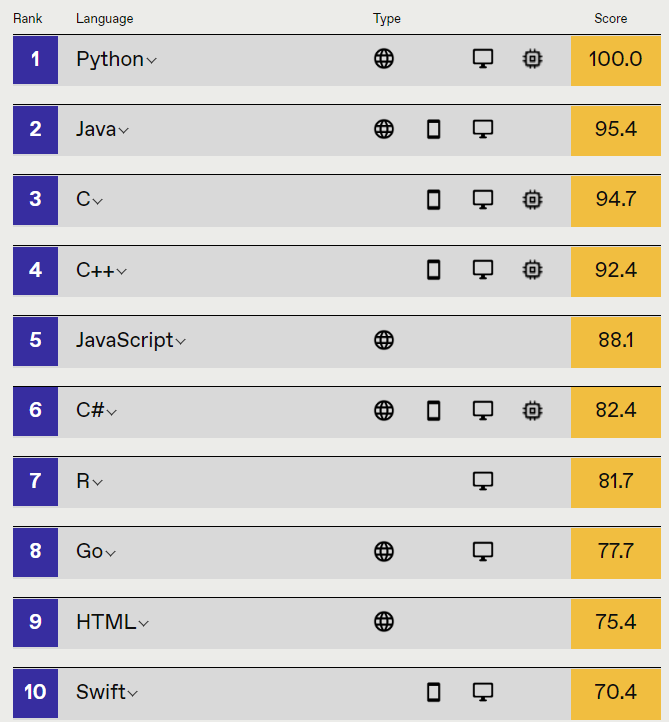
\includegraphics[width=2.60417in,height=\textheight]{images/01/toplanguage2021.png}
\caption{\url{https://spectrum.ieee.org/top-programming-languages/}}
\end{figure}

R은 데이터를 통계분석에 널리 사용되는데 이는 데이터를 눈으로 확인하기 위한 visualization 이나 벡터 연산 등의 강력한 기능 때문에 점점 더 많은 사람들이 사용하고 있습니다. 기존에는 속도나 확장성이 다른 언어들에 비해 단점으로 지적되었으나 R 언어의 계속적인 개발과 업데이트로 이러한 단점들이 빠르게 보완되고 있습니다. R 사용을 위해서는 R 언어의 코어 프로그램을 먼저 설치하고 그 다음 R 언어용 IDE(Integrated Development Environment)인 RStudio 설치가 필요합니다.


\includegraphics[width=1.5625in,height=\textheight]{images/01/rstudio.png}

Rstudio는 R 언어를 위한 오픈소스 기반 통합개발환경(IDE)으로 R 프로그래밍을 위한 편리한 기능들을 제공해 줍니다. R언어가 주목을 받고 두터운 사용자 층을 확보할 수 있게된 핵심 동력이 Rstudio 입니다. 자체적으로 최고수준의 오픈소스 개발팀이 있으며 \texttt{tidyverse}, `\texttt{,}shiny` 등의 데이터 분석 관련 주요 패키지를 개발하였고 정기적으로 conference 개최를 하면서 기술 보급의 핵심 역할을 하고 있습니다.

\begin{figure}
\centering
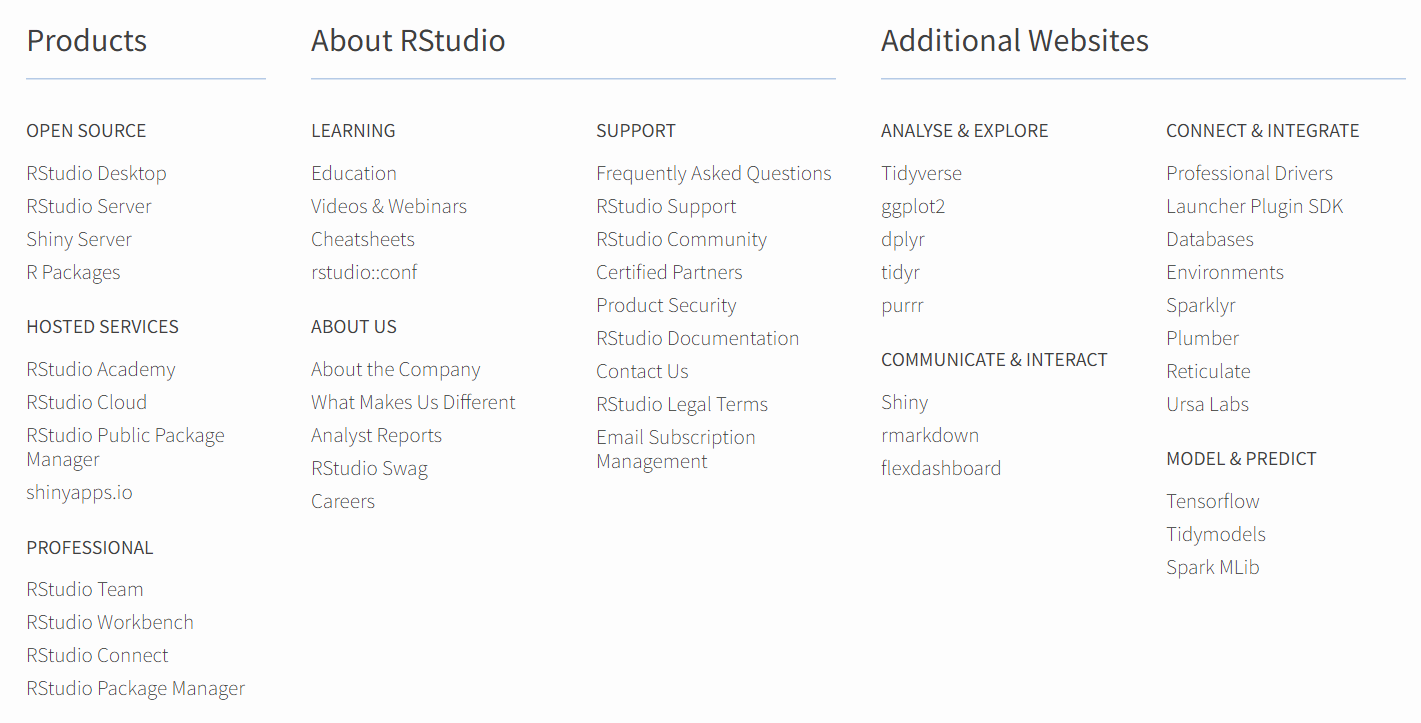
\includegraphics[width=5.72917in,height=\textheight]{images/01/rstudiobottom.png}
\caption{\url{https://www.rstudio.com/}}
\end{figure}

\hypertarget{r-rstudio-installation}{%
\section{R / Rstudio Installation}\label{r-rstudio-installation}}

\hypertarget{r-uxc124uxce58}{%
\subsection{R 설치}\label{r-uxc124uxce58}}

\begin{itemize}
\tightlist
\item
  R 사이트에 접속 후 (\url{https://www.r-project.org/}) 좌측 메뉴 상단에 위치한 CRAN 클릭.
\item
  미러 사이트 목록에서 Korea의 아무 사이트나 들어감
\item
  Download R for Windows를 클릭 후 base 링크 들어가서
\item
  Download R x.x.x for Windows 링크 클릭으로 실행 프로그램 다운로드
\item
  로컬 컴퓨터에 Download 된 R-x.x.x-win.exe 를 실행 (2022.5 현재 R 버전은 4.2.0).
\item
  설치 프로그램의 지시에 따라 R 언어 소프트웨어 설치를 완료
\end{itemize}

\hypertarget{rstudio-uxc124uxce58}{%
\subsection{Rstudio 설치}\label{rstudio-uxc124uxce58}}

\begin{itemize}
\tightlist
\item
  사이트에 접속 (\url{https://www.rstudio.com/}), 상단의 Products \textgreater{} RStudio 클릭
\item
  RStudio Desktop 선택
\item
  Download RStudio Desktop 클릭
\item
  RStudio Desktop Free 버전의 Download를 선택하고
\item
  Download RStudio for Windows 클릭, 다운로드
\item
  로컬 컴퓨터에 다운로드된 RStudio-x.x.x.exe 실행 (2022.5 현재 RStudio Desktop 2022.02.2+485)
\item
  설치 가이드에 따라 설치 완료
\end{itemize}

\hypertarget{rstudio-interface}{%
\section{Rstudio interface}\label{rstudio-interface}}

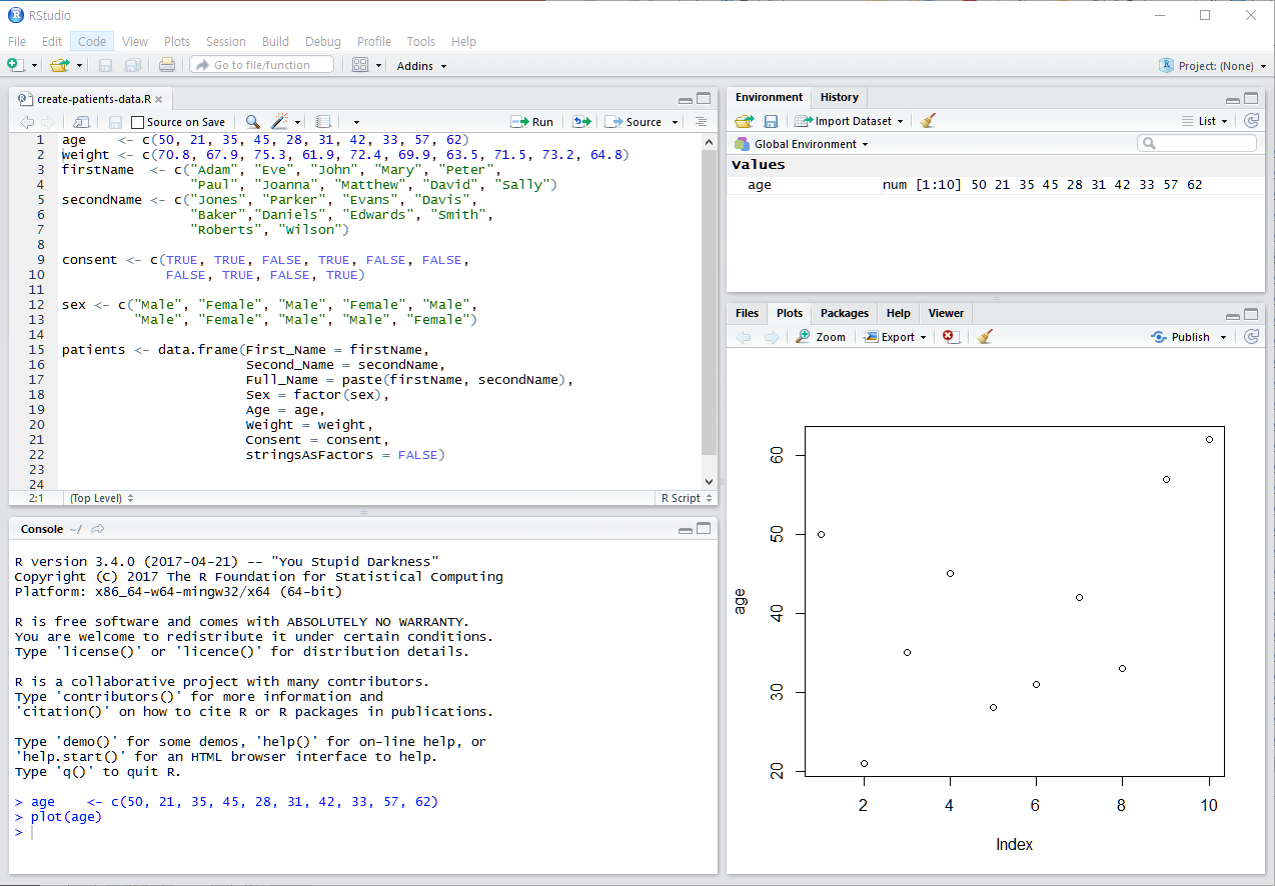
\includegraphics[width=5.20833in,height=\textheight]{images/01/01-11.PNG}

\begin{itemize}
\tightlist
\item
  기본 화면에서 좌측 상단의 공간은 코드편집창, 좌측 하단은 콘솔창
\item
  각 위치를 기호에 따라서 바꿀 수 있음 (View --\textgreater{} Pane)
\end{itemize}

\hypertarget{keyboard-shortcuts}{%
\subsection{Keyboard shortcuts}\label{keyboard-shortcuts}}

\begin{itemize}
\tightlist
\item
  참고사이트

  \begin{itemize}
  \tightlist
  \item
    \url{https://support.rstudio.com/hc/en-us/articles/200711853-Keyboard-Shortcuts}
  \item
    Tools --\textgreater{} Keyboard shortcut Quick Reference (\texttt{Alt\ +\ Shift\ +\ K})
  \end{itemize}
\item
  코드편집창 이동 (\texttt{Ctrl\ +\ 1}) 콘솔창 이동(\texttt{Ctrl\ +\ 2})
\item
  한 줄 실행 (\texttt{Ctrl\ +\ Enter})
\item
  저장 (\texttt{Ctrl\ +\ S})
\item
  주석처리 (\texttt{Ctrl\ +\ Shift\ +\ C})

  \begin{itemize}
  \tightlist
  \item
    또는 \texttt{\#}으로 시작하는 라인
  \end{itemize}
\item
  텝 이동 (\texttt{Ctrl\ +\ F11}, \texttt{Ctrl\ +\ F12})
\item
  코드편집창 확대 (\texttt{Shift\ +\ Ctrl\ +\ 1}) 콘솔창 확대 (\texttt{Shift\ +\ Ctrl\ +\ 2})
\item
  컬럼 편집 (\texttt{Alt\ +\ 마우스\ 드레그})
\item
  자동 완성 기능 (Tab completion) in RStudio
\end{itemize}

\textbf{Exercises}

\begin{enumerate}
\def\labelenumi{\arabic{enumi}.}
\tightlist
\item
  코드편집창에서 다음을 입력/실행하고 단축키를 사용하여 주석을 넣으시오
\end{enumerate}

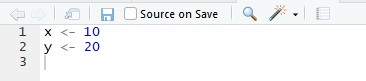
\includegraphics{images/01/01-14.PNG}

\begin{itemize}
\tightlist
\item
  단축키 \texttt{Ctrl\ +\ enter}로 코드 실행
\item
  단축키 \texttt{Ctrl\ +\ 2}로 커서 콘솔창으로 이동
\item
  \texttt{x}값 \texttt{x+y}값 확인
\item
  단축키 \texttt{Ctrl\ +\ 1}로 코드편집창 이동
\item
  단축키 \texttt{Ctrl\ +\ Shift\ +\ C} 사용
\end{itemize}

\begin{Shaded}
\begin{Highlighting}[]
\CommentTok{\# x \textless{}{-} 10}
\CommentTok{\# y \textless{}{-} 20}
\end{Highlighting}
\end{Shaded}

\hypertarget{environment-and-files}{%
\subsection{Environment and Files}\label{environment-and-files}}

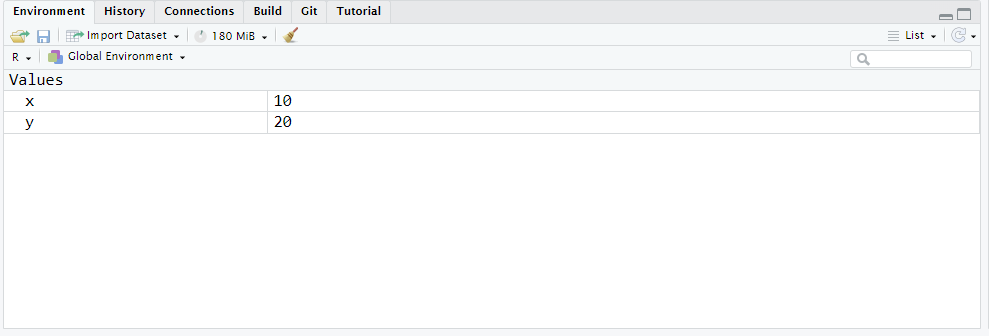
\includegraphics[width=4.16667in,height=\textheight]{images/01/envandhist.png}

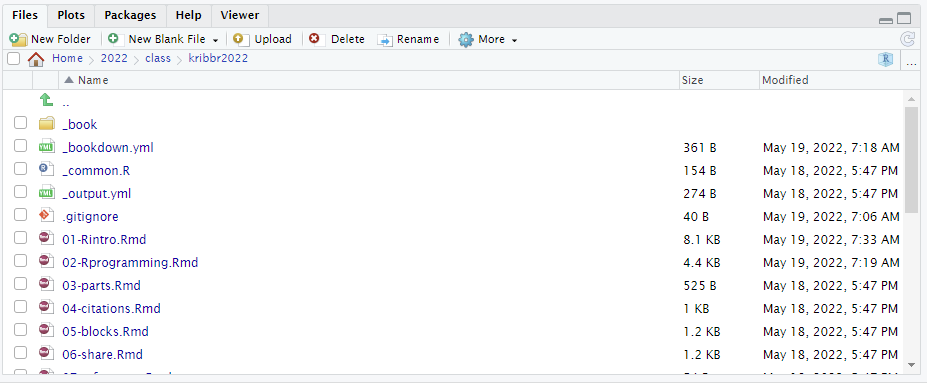
\includegraphics[width=4.16667in,height=\textheight]{images/01/fileandpackages.png}

\hypertarget{start-a-project}{%
\section{Start a project}\label{start-a-project}}

프로젝트를 만들어서 사용할 경우 파일이나 디렉토리, 내용 등을 쉽게 구분하여 사용 가능합니다. 아래와 같이 임의의 디렉토리에 \texttt{kribbR} 이라는 디렉토리를 생성하고 \texttt{lecture1} 프로젝트를 만듭니다.

\begin{quote}
File \textgreater{} New Project \textgreater{} New Directory \textgreater{} New Project \textgreater{} ``kribbR'' \textgreater{} Create Project
\end{quote}

시작할 때는 해당 디렉토리의 \texttt{xxx.Rproj} 파일을 클릭합니다. Rstudio 오른쪽 상단 프로젝트 선택을 통해서 빠르게 다른 프로젝트의 작업공간으로 이동할 수 있습니다.

\hypertarget{hello-world}{%
\subsection{Hello world}\label{hello-world}}

\begin{quote}
File \textgreater{} New File \textgreater{} R markdown \textgreater{} OK
\end{quote}

\begin{Shaded}
\begin{Highlighting}[]
\NormalTok{mystring }\OtherTok{\textless{}{-}} \StringTok{"Hello }\SpecialCharTok{\textbackslash{}n}\StringTok{ world!"}
\FunctionTok{cat}\NormalTok{(mystring)}
\FunctionTok{print}\NormalTok{(mystring)}
\end{Highlighting}
\end{Shaded}

\hypertarget{getting-help}{%
\section{Getting help}\label{getting-help}}

R은 방대한 양의 도움말 데이터를 제공하며 다음과 같은 명령어로 특정 함수의 도움말과 예제를 찾아볼 수 있습니다. \texttt{?} 명령을 사용하면 되며 구글이나 웹에서도 도움을 얻을 수 있습니다.

\begin{Shaded}
\begin{Highlighting}[]
\FunctionTok{help}\NormalTok{(}\StringTok{"mean"}\NormalTok{)}
\NormalTok{?mean}
\FunctionTok{example}\NormalTok{(}\StringTok{"mean"}\NormalTok{)}
\FunctionTok{help.search}\NormalTok{(}\StringTok{"mean"}\NormalTok{)}
\NormalTok{??mean}
\FunctionTok{help}\NormalTok{(}\AttributeTok{package=}\StringTok{"MASS"}\NormalTok{)}
\end{Highlighting}
\end{Shaded}

또한 \url{https://www.rstudio.com/resources/cheatsheets/} 에서는 다양한 R언어의 기능을 한 눈에 알아볼 수 있게 만든 cheatsheet 형태의 문서를 참고할 수 있습니다.

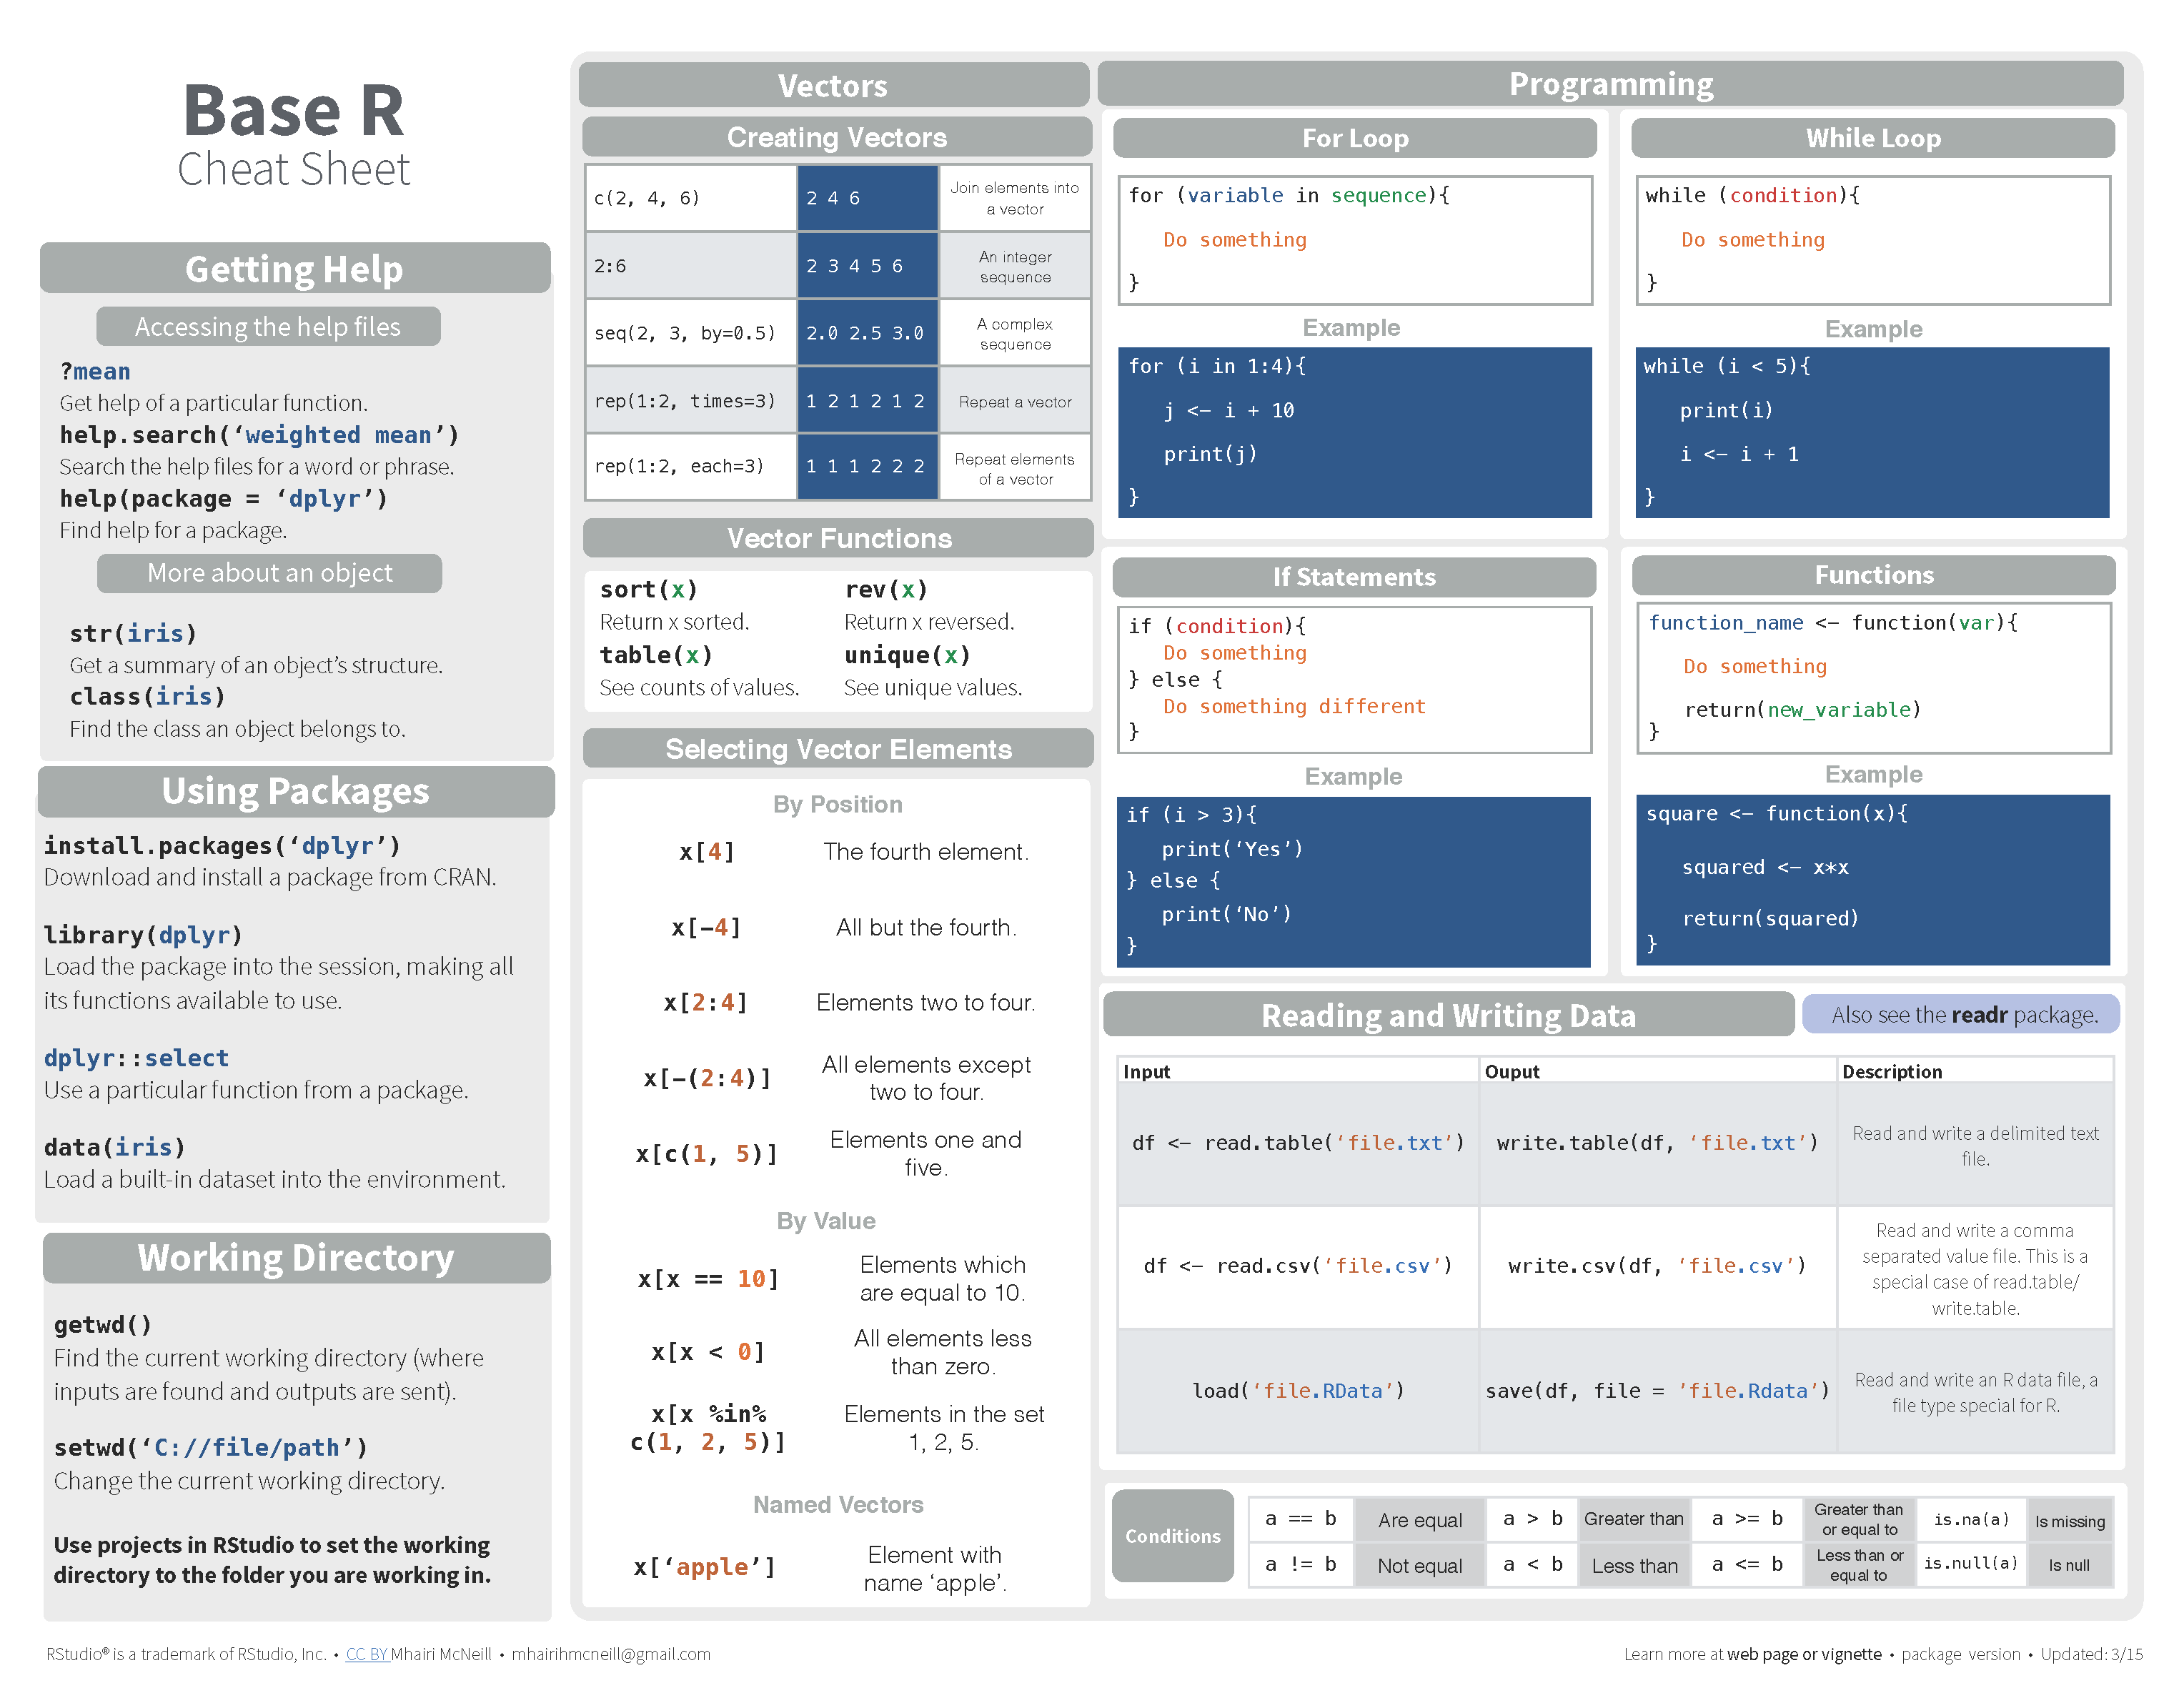
\includegraphics[width=5.72917in,height=\textheight]{images/01/base-r_1.png}
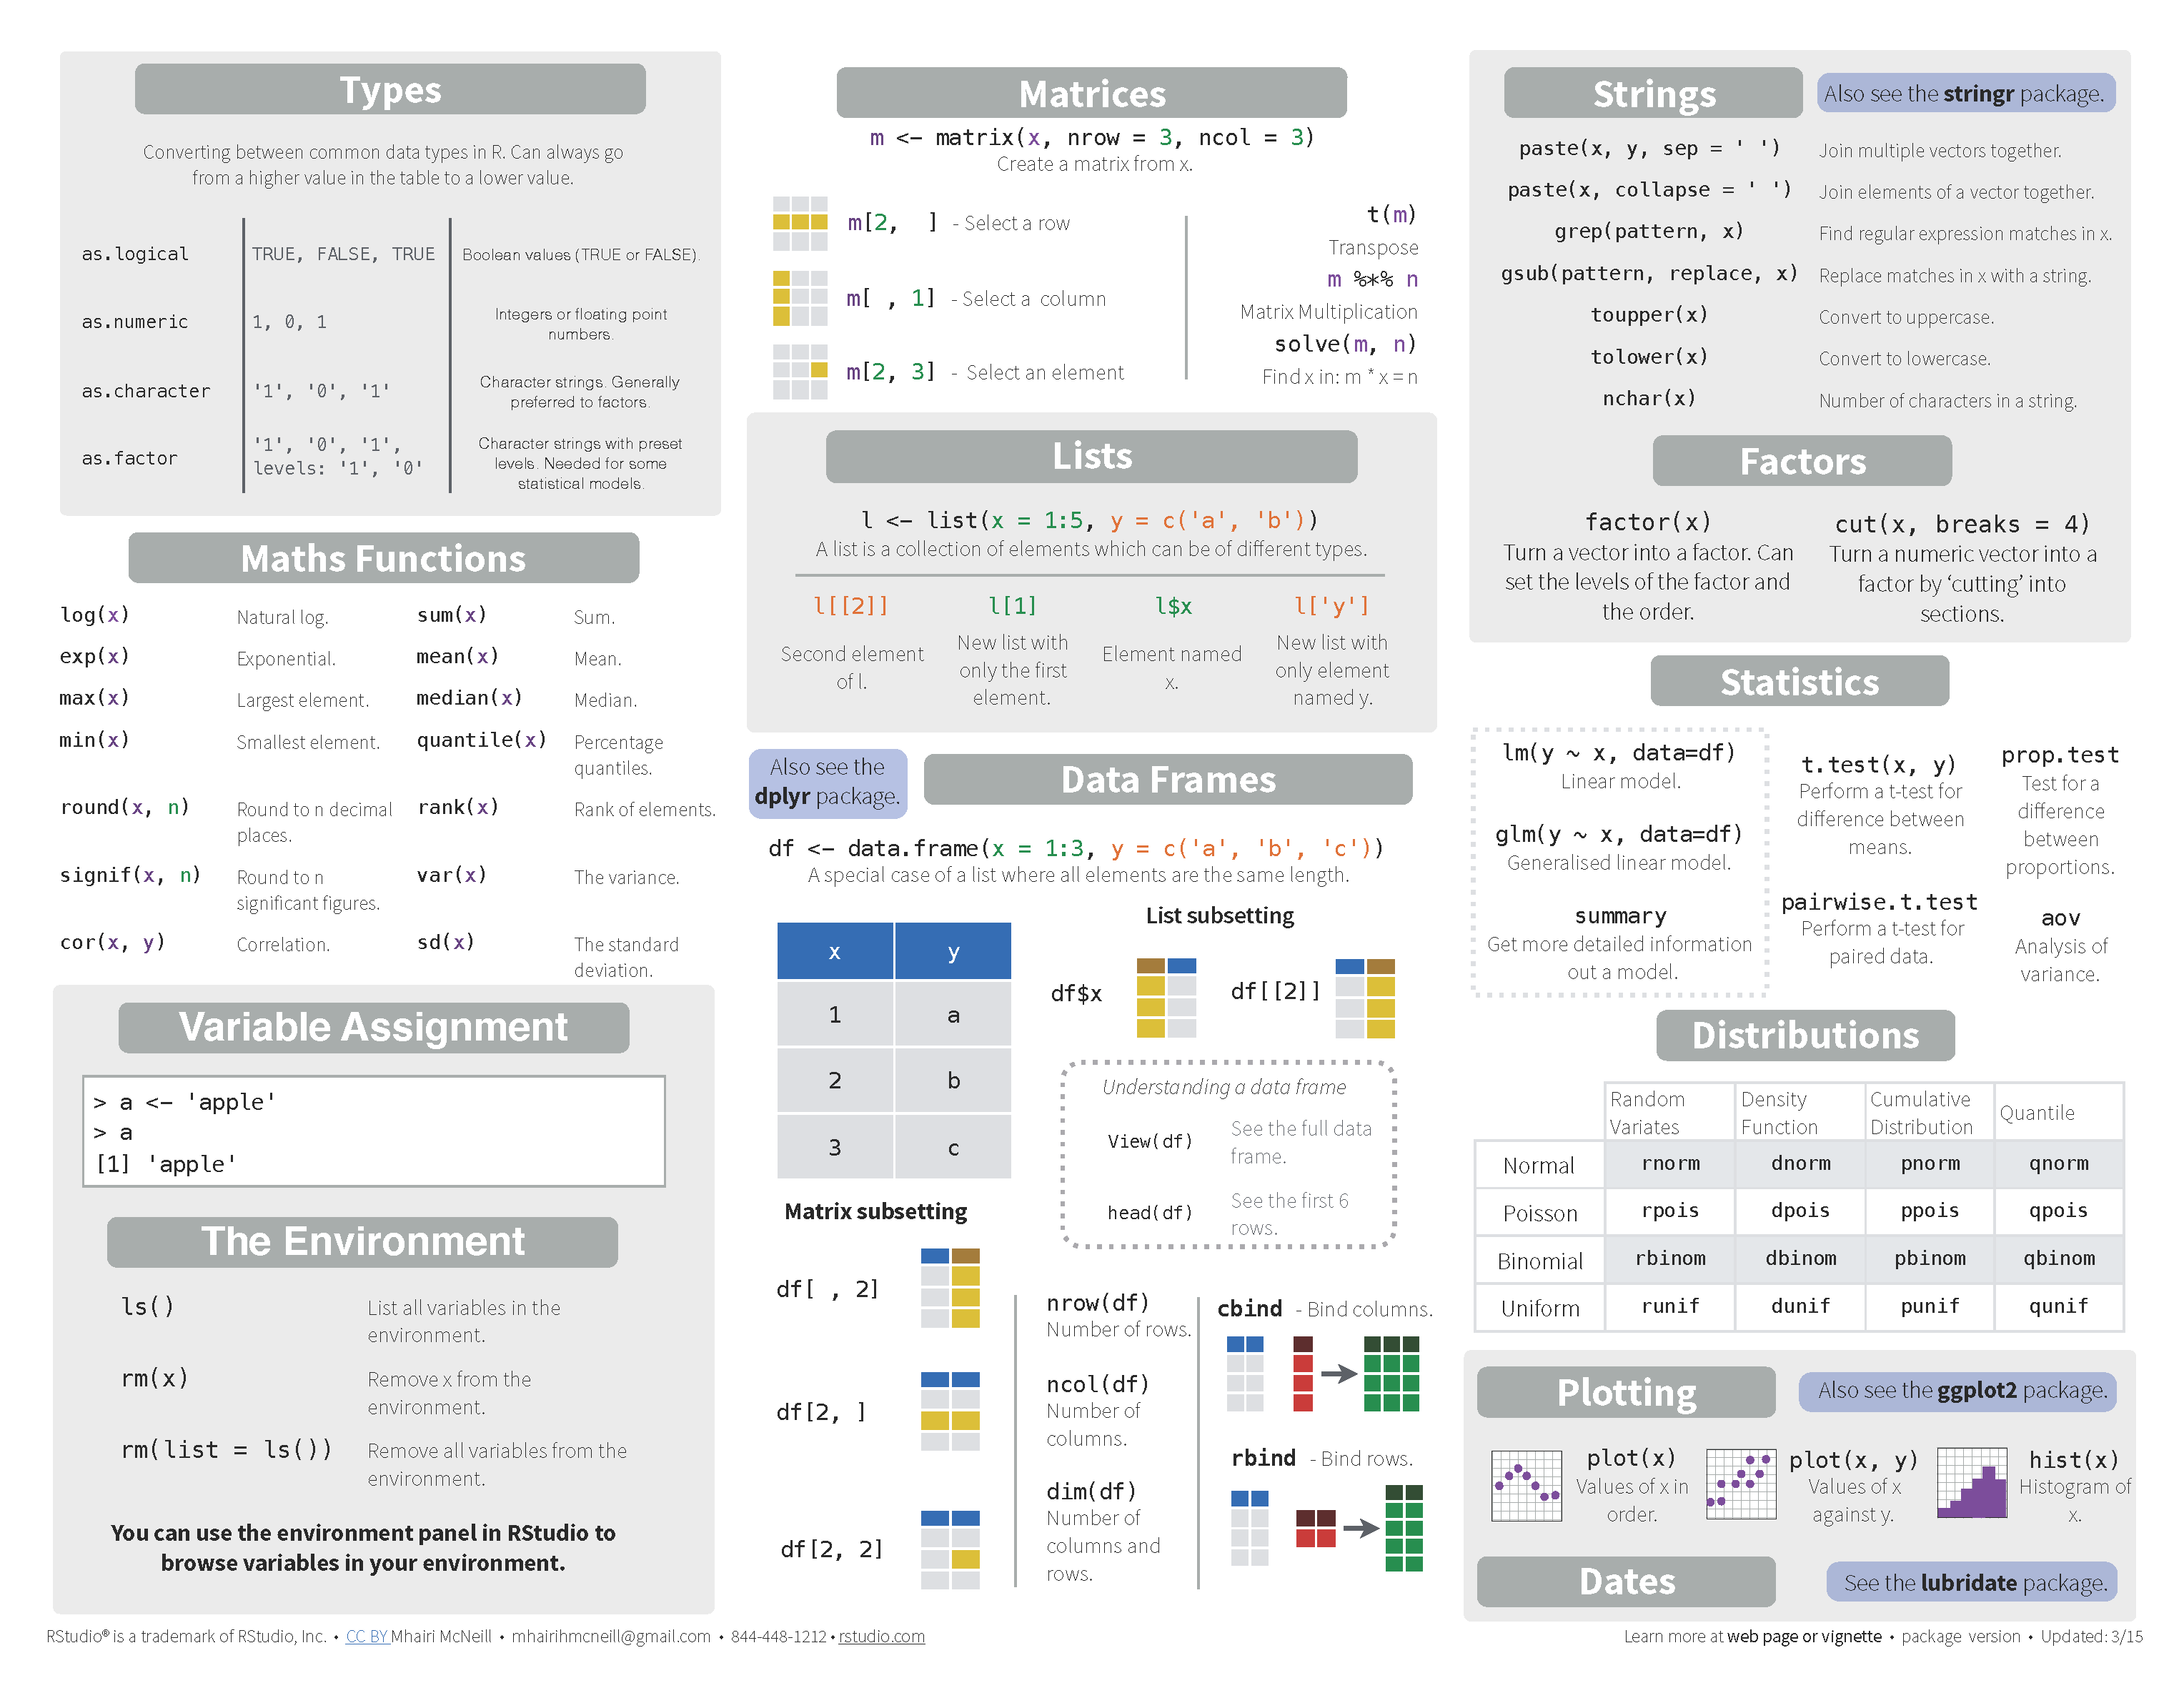
\includegraphics[width=5.72917in,height=\textheight]{images/01/base-r_2.png}

\hypertarget{r-packages-and-dataset}{%
\section{R packages and Dataset}\label{r-packages-and-dataset}}

R 패키지는 함수와 데이터셋의 묶음으로 다른 사람들이 만들어 놓은 코드나 기능을 가져와서 사용하므로써 코드 작성의 수고로움을 줄이고 편리하고 검증된 함수(기능)를 빠르게 도입하여 사용할 수 있다는 장점이 있습니다. 예를 들어 \texttt{sd()} 함수는 \texttt{stats} package에서 제공하는 함수로써 표준편차 계산을 위한 별도의 함수를 만들어서 사용할 필요가 없이 바로 (stats 패키지는 R 기본 패키지로) 별도 설치 없이 바로 사용 가능합니다.

이러한 패키지는 인터넷의 \texttt{repository}에서 구할 수 있으며 대표적인 \texttt{repository}는 The Comprehensive R Archive Network (CRAN) (\url{http://cran.r-project.org/web/views/}) 와 생물학자를 위한 Bioconductor (\url{http://www.bioconductor.org/}) 가 있습니다. 이러한 패키지의 설치는 아래와 같이 RStudio를 이용하거나 콘솔창에서 \texttt{install.packages()} 함수를 이용할 수 있습니다.

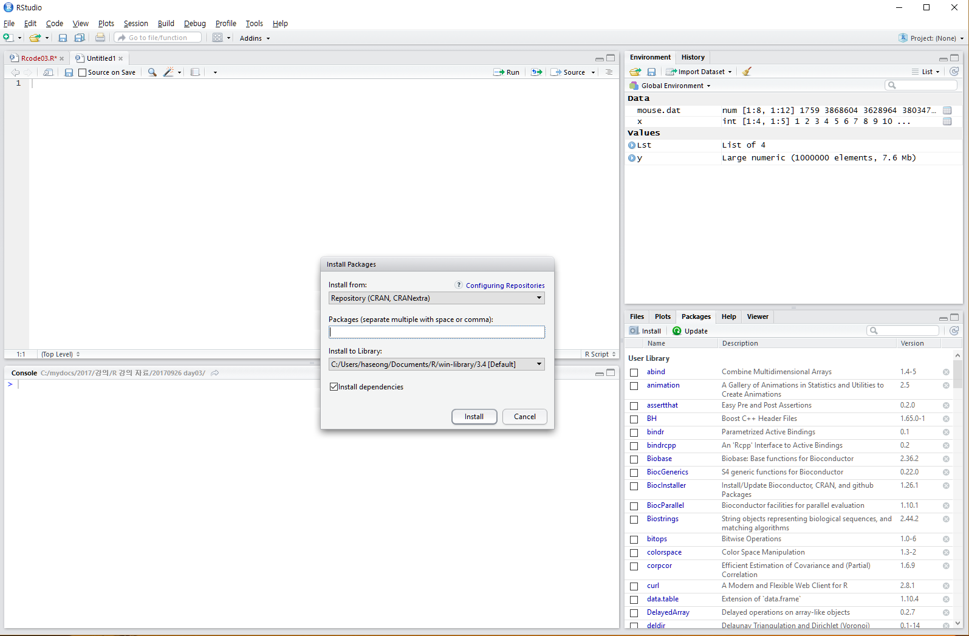
\includegraphics[width=4.6875in,height=\textheight]{images/01/01-18.PNG}

패키지를 설치하고 사용하기 위해서는 \texttt{library()} 함수를 사용해서 관련 명령어를 사용하기 전에 미리 loading 해 두어야 합니다. 한 번 로딩으로 작업 세션이 끝날때까지 관련된 함수를 사용할 수 있으나 R 세션이나 RStudio를 재시작 할 경우 다시 로딩해야 사용할 수 있습니다.

\begin{Shaded}
\begin{Highlighting}[]
\FunctionTok{library}\NormalTok{(UsingR)}
\end{Highlighting}
\end{Shaded}

\begin{itemize}
\tightlist
\item
  R 설치 디렉토리
\item
  R 패키지 설치 디렉토리
\end{itemize}

\begin{Shaded}
\begin{Highlighting}[]
\FunctionTok{.libPaths}\NormalTok{()}
\FunctionTok{path.package}\NormalTok{()}
\end{Highlighting}
\end{Shaded}

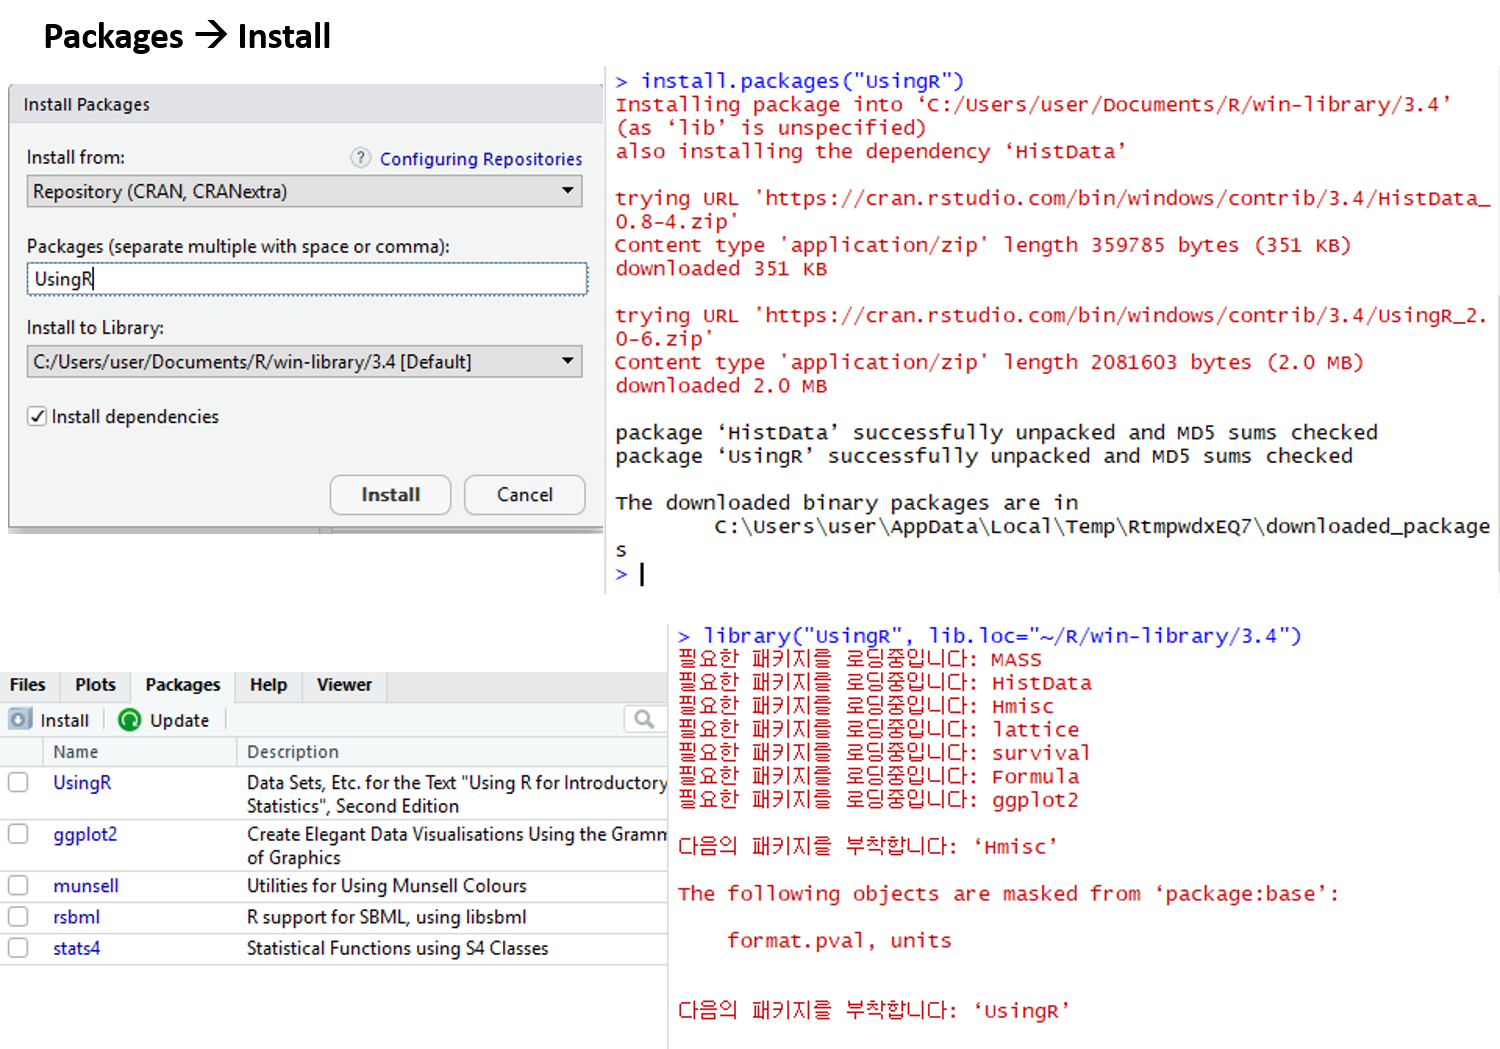
\includegraphics[width=4.6875in,height=\textheight]{images/01/01-19.PNG}

일반적으로 패키지 안에 관련된 데이터도 같이 저장되어 있으며 \texttt{data()} 함수를 이용해서 패키지 데이터를 사용자 작업공간에 복사해서 사용 가능합니다.

\begin{Shaded}
\begin{Highlighting}[]
\FunctionTok{head}\NormalTok{(rivers)}
\FunctionTok{length}\NormalTok{(rivers)}
\FunctionTok{class}\NormalTok{(rivers)}
\FunctionTok{data}\NormalTok{(rivers)}
\FunctionTok{data}\NormalTok{(}\AttributeTok{package=}\StringTok{"UsingR"}\NormalTok{)}
\FunctionTok{library}\NormalTok{(HistData)}
\FunctionTok{head}\NormalTok{(Cavendish)}
\FunctionTok{str}\NormalTok{(Cavendish)}
\FunctionTok{head}\NormalTok{(Cavendish}\SpecialCharTok{$}\NormalTok{density2)}
\end{Highlighting}
\end{Shaded}

\begin{center}\rule{0.5\linewidth}{0.5pt}\end{center}

이 저작물은 크리에이티브 커먼즈 저작자표시-비영리-변경금지 4.0 국제 라이선스에 따라 이용할 수 있습니다.

\hypertarget{rmarkdown}{%
\chapter{Rmarkdown}\label{rmarkdown}}

Rmarkdown은 데이터를 분석하는 코드와 리포트를 동시에 수행할 수 있는 일종의 통합 문서입니다. 워드나 아래한글에서 프로그래밍과 데이터분석을 위한 코드를 작성할 수 있는 경우라고 생각해도 됩니다. Plain-text 기반의 markdown 문법을 사용하며 Rmarkdown으로 작성된 문서는 HTML, PDF, MS word, Beamer, HTML5 slides, books, website 등 다양한 포멧의 출력물로 변환할 수 있습니다.

\begin{figure}
\centering
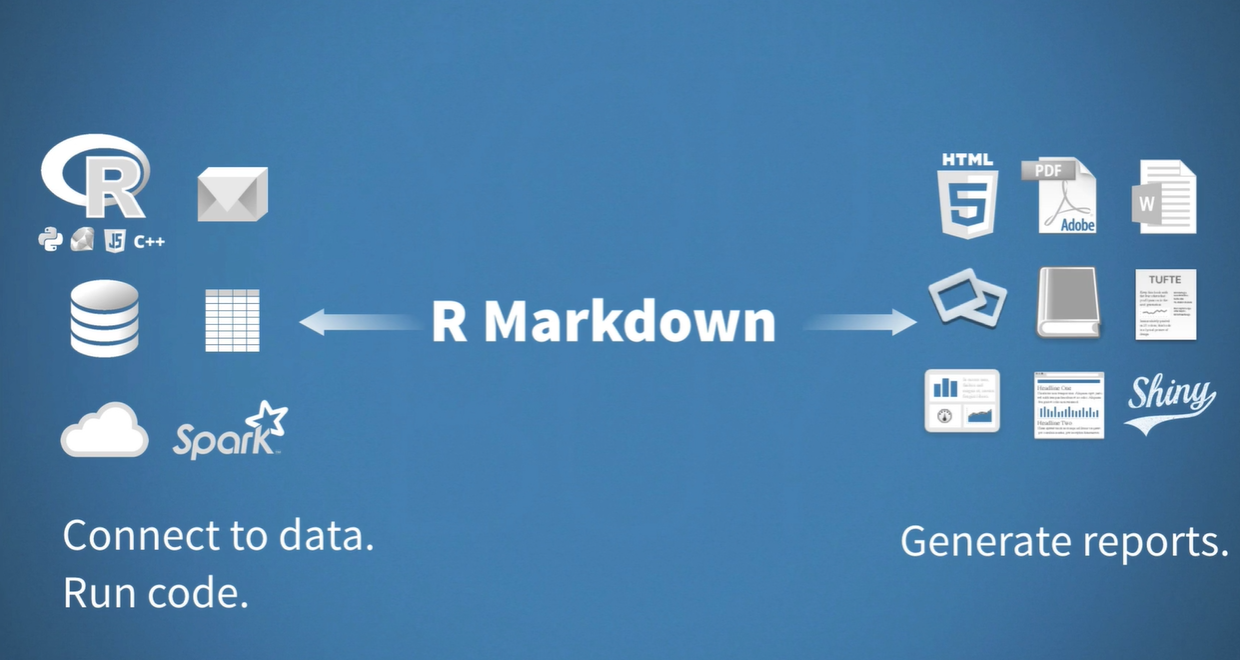
\includegraphics[width=5.20833in,height=\textheight]{images/rmarkdown/rmarkdown-01.PNG}
\caption{Image from rmarkdown.rstudio.com}
\end{figure}

Rmarkdown 웹사이트에 Rmarkdown 소개 동영상과 \href{https://rmarkdown.rstudio.com/lesson-1.html}{Rmarkdown 공식 사이트 메뉴얼} 관련 서적 \href{https://bookdown.org/yihui/rmarkdown/}{Rmarkdown: The Definitive Guide}를 참고하세요. 또한 Rmarkdown을 사용할 때 \href{https://github.com/rstudio/cheatsheets/raw/master/rmarkdown-2.0.pdf}{cheatsheet}를 옆에 두고 수시로 보면서 사용하시면 많은 도움이 될 수 있습니다.

\hypertarget{rmarkdownuxc758-uxae30uxbcf8-uxc791uxb3d9-uxc6d0uxb9ac}{%
\section{Rmarkdown의 기본 작동 원리}\label{rmarkdownuxc758-uxae30uxbcf8-uxc791uxb3d9-uxc6d0uxb9ac}}

Rmarkdown은 plain text 기반으로 작성되며 Rmd 라는 확장자를 갖는 파일로 저장됩니다. 다음과 같은 텍스트 파일이 Rmd 파일의 전형적인 예 입니다.

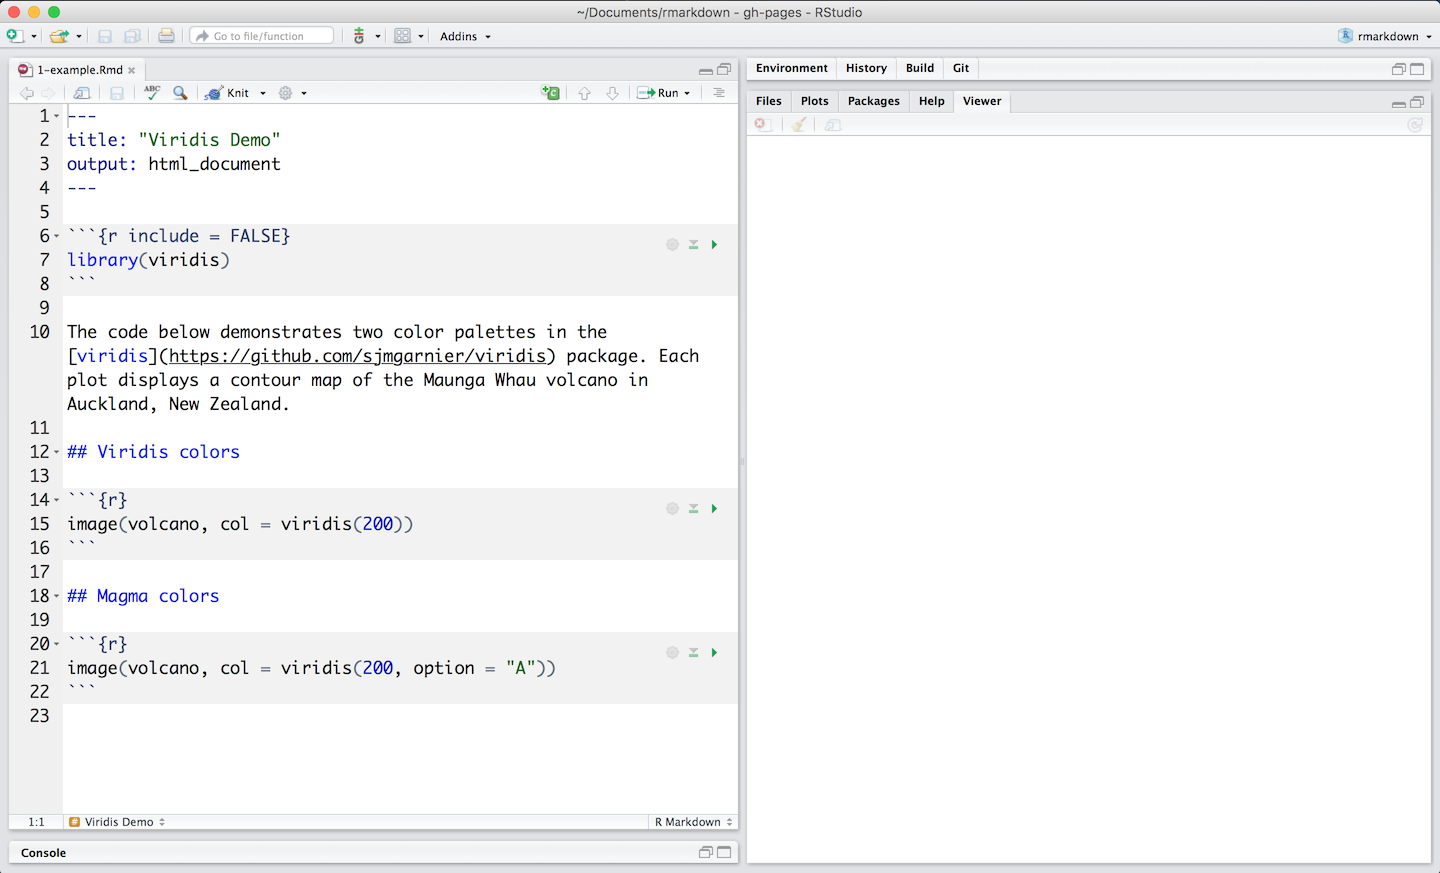
\includegraphics[width=5.20833in,height=\textheight]{images/rmarkdown/how-1-file.png}

위 예제에서 네 가지 다른 종류의 컨텐츠를 볼 수 있습니다. 하나는 - - - 으로 둘러쌓인 내용으로 YAML 이라고 하며 JSON과 같은 데이터 직렬화를 수행하는 하나의 데이터 저장 포멧입니다. 백틱(`) 으로 둘러쌓인 코드청그(Code Chunks)라고 하는 부분에는 R이나 python 등의 다양한 코드(실재 작동하는)를 넣어서 사용합니다. 그리고 \#\#\# 으로 표시된 글은 제목 글을 나타내며 나머지는 일반적인 텍스트를 나타냅니다.

\begin{verbatim}
---
title: "Lecture3"
output:
  html_document:
    toc: yes
    toc_float: yes
    toc_depth: 2
    number_sections: yes
---
\end{verbatim}

이러한 Rmarkdown 파일은 \texttt{render}라는 명령어로 원하는 포맷의 문서로 변환할 수 있습니다. 다음 예의 파일을 pdf 형식으로 rendering 하기 위해서는 YAML에 pdf 임을 명시하고 아래와 같이 \texttt{render}함수를 사용하면 됩니다. 또는 Rstudio 코드 입력창 상단의 Knit 버튼으로 pdf나 html 문서를 생성할 수 있습니다.

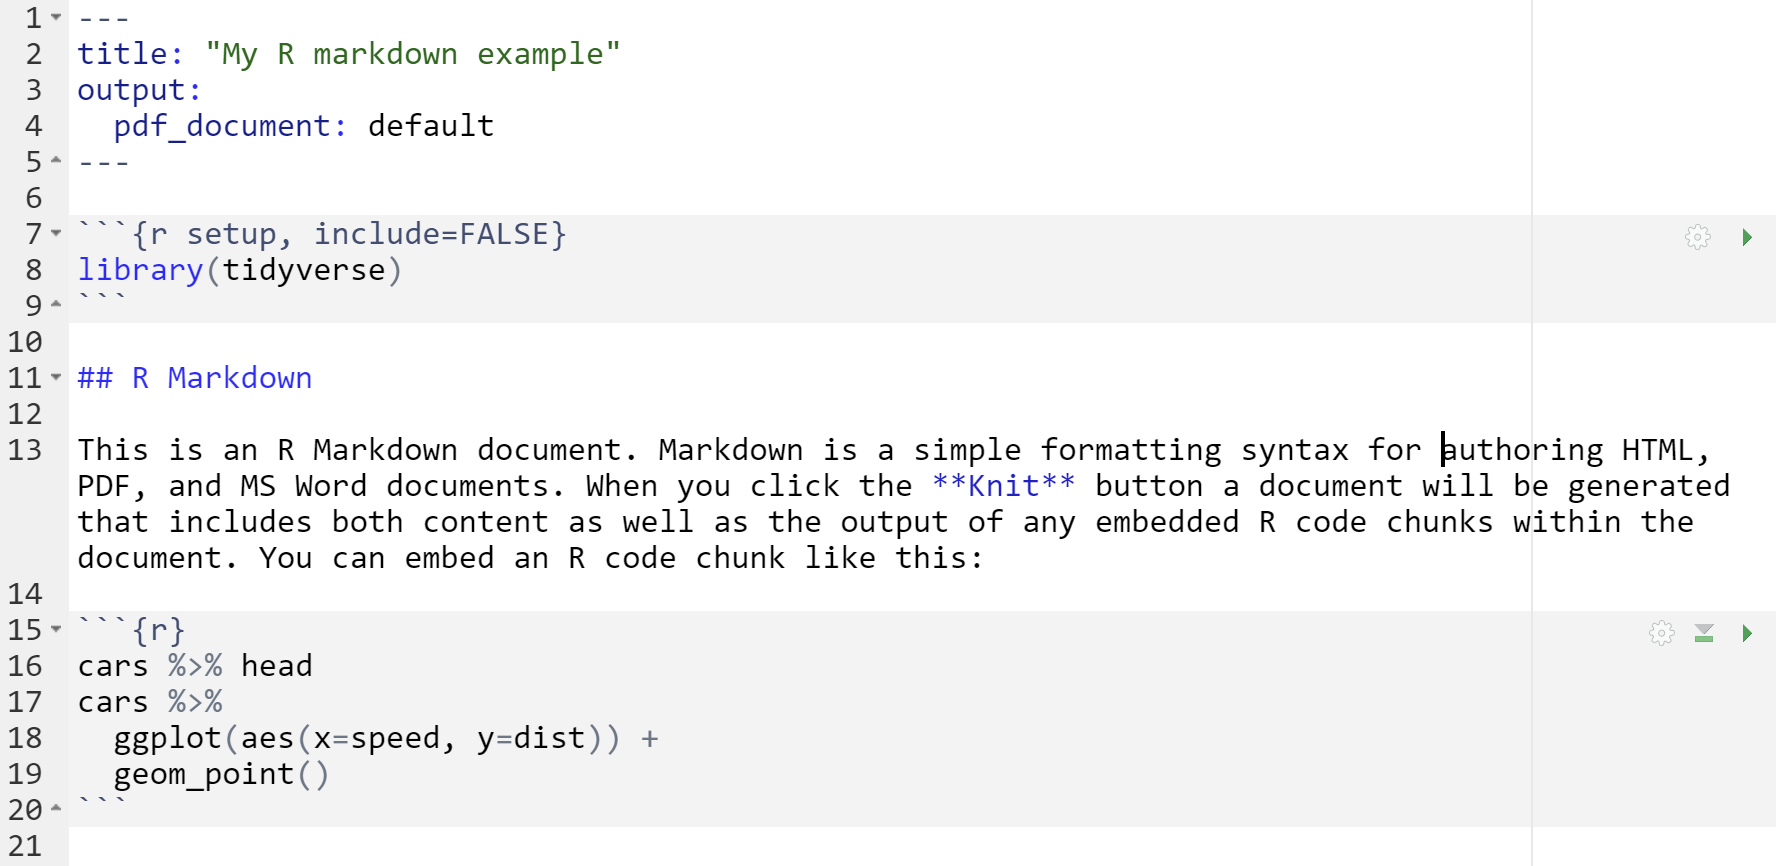
\includegraphics[width=5.20833in,height=\textheight]{images/rmarkdown/example2.PNG}

\begin{Shaded}
\begin{Highlighting}[]
\FunctionTok{render}\NormalTok{(}\StringTok{"examples/test.Rmd"}\NormalTok{, }\AttributeTok{output\_format =} \StringTok{"pdf\_document"}\NormalTok{)}
\end{Highlighting}
\end{Shaded}

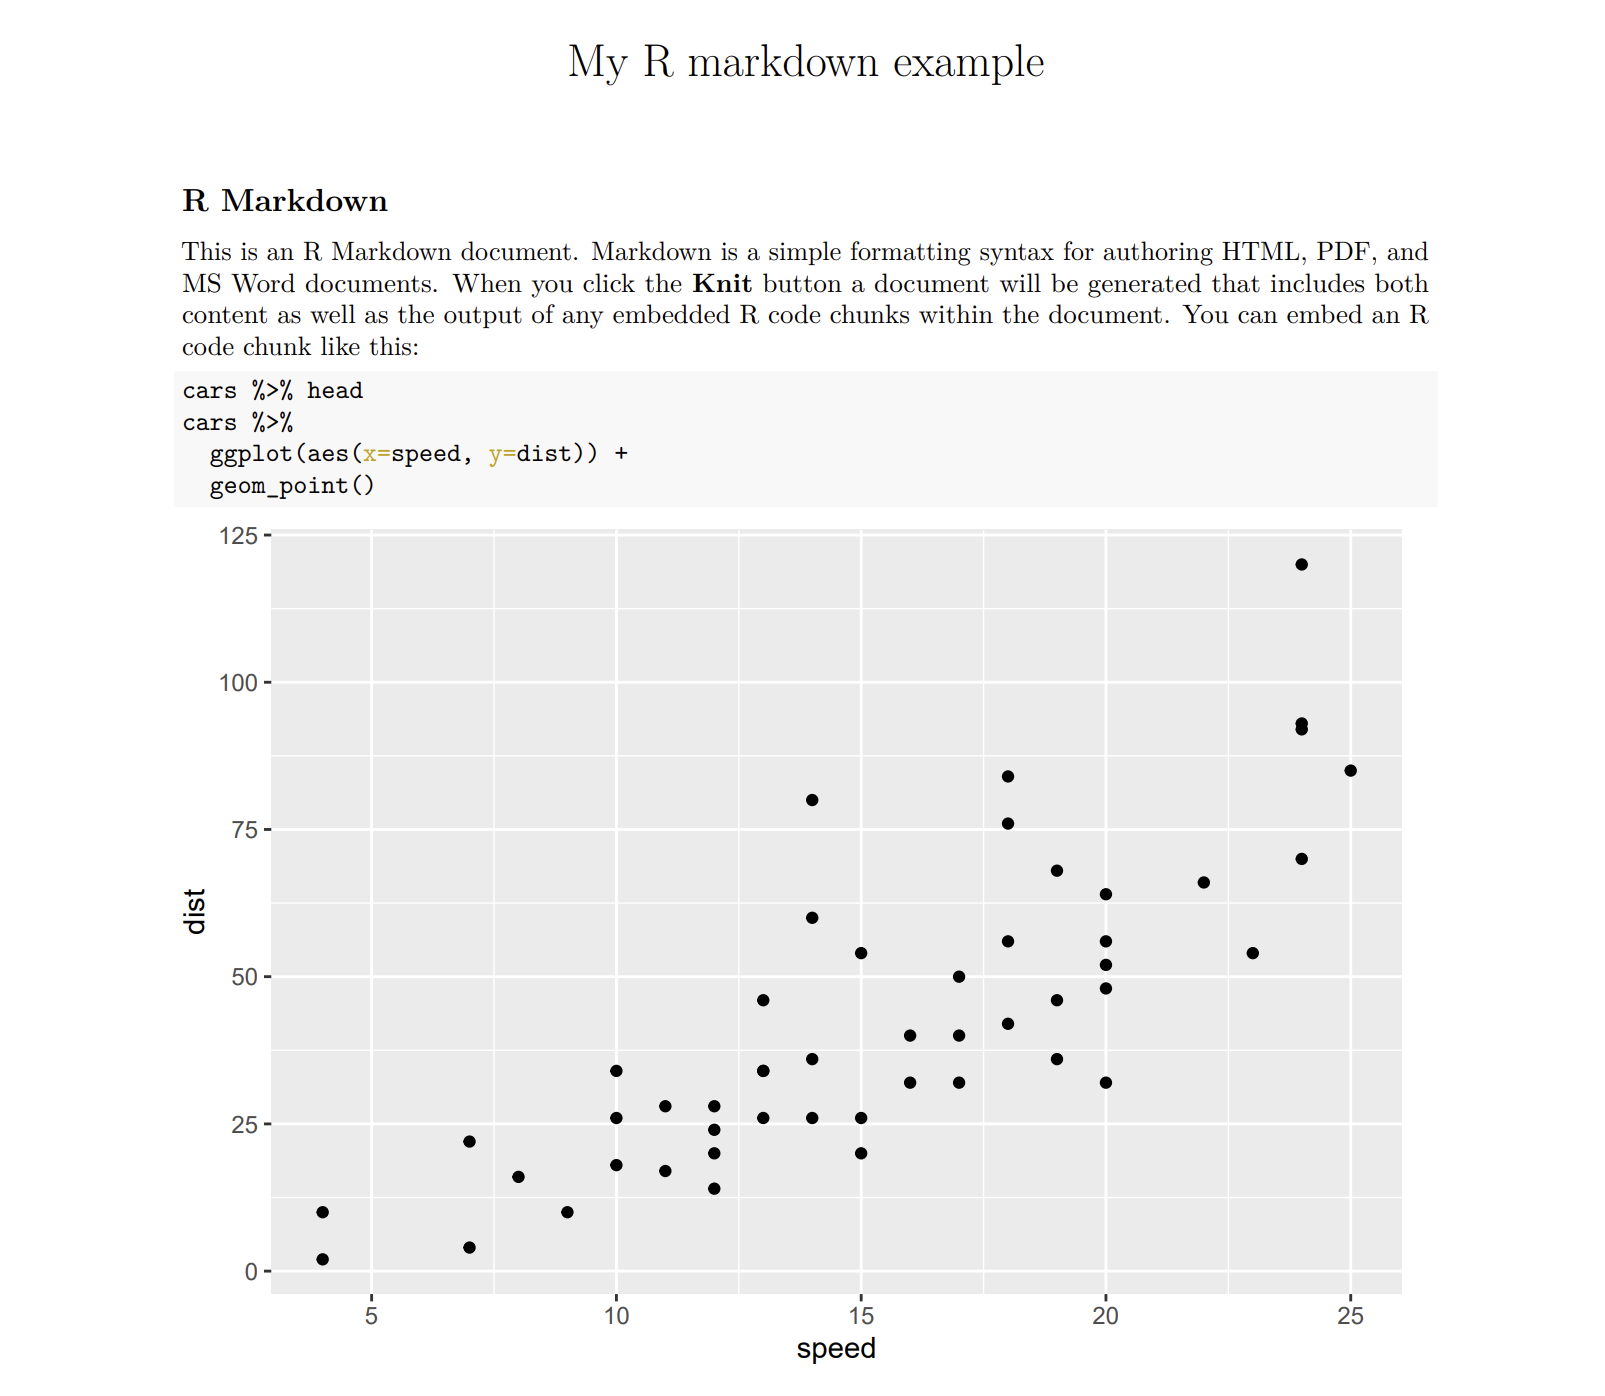
\includegraphics[width=4.6875in,height=\textheight]{images/rmarkdown/ex_pdf.PNG}

Rmarkdown의 작동 원리는 Rmd 파일을 만든 후 \texttt{render} 함수를 부르면 \href{https://yihui.org/knitr/}{knitr} 소프트웨어가 R 코드를 실행시킨 후 markdown (.md) 파일을 생성합니다. 이 후 .md 파일을 \href{https://pandoc.org/}{pandoc} 이라는 문서변환기가 원하는 문서 형태로 전환해 줍니다.

\hypertarget{uxcf54uxb4dc-uxc785uxb825}{%
\section{코드 입력}\label{uxcf54uxb4dc-uxc785uxb825}}

Rmarkdown에서 사용하는 코드청크는 \texttt{CTRL+ALT+i} 단축키를 사용해서 넣을 수 있으며 다음과 같은 몇 가지 옵션으로 코드 스니펫들의 실행/숨김 여부를 결정할 수 있습니다.

\begin{itemize}
\tightlist
\item
  \texttt{include\ =\ FALSE} : 코드는 실행되지만 보고서에 결과와 코드가 보여지지 않음
\item
  \texttt{echo\ =\ FALSE} : 코드는 실행되고 보고서에 결과가 포함되지만 코드는 보여지지 않음
\item
  \texttt{eval\ =\ FALSE} : 코드가 실행되지 않지만 보고서에 코드는 보여짐
\item
  \texttt{message\ =\ FALSE}, \texttt{warning=FALSE}, \texttt{error=FALSE} : 코드에 의해서 발생되는 메세지/경고/에러가 보고서에 보여지지 않음
\item
  \texttt{fig.cap\ =\ "..."} : 코드로 그려지는 그래프에 캡션을 붙일 수 있음
\end{itemize}

\begin{figure}
\centering
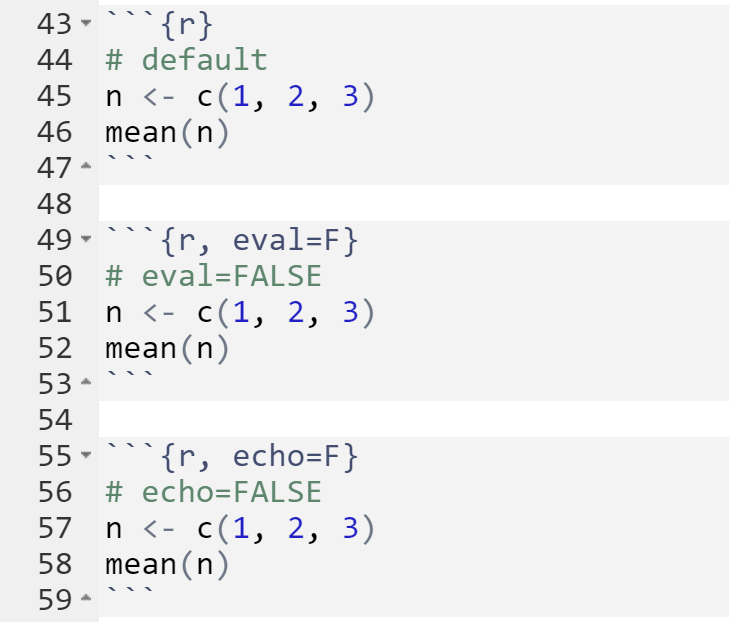
\includegraphics[width=2.60417in,height=\textheight]{images/rmarkdown/codechunk1.PNG}
\caption{코드청크 옵션 예시}
\end{figure}

실행 결과는 아래와 같습니다.

\begin{Shaded}
\begin{Highlighting}[]
\CommentTok{\# default}
\NormalTok{n }\OtherTok{\textless{}{-}} \FunctionTok{c}\NormalTok{(}\DecValTok{1}\NormalTok{, }\DecValTok{2}\NormalTok{, }\DecValTok{3}\NormalTok{)}
\FunctionTok{mean}\NormalTok{(n)}
\CommentTok{\#\textgreater{} [1] 2}
\end{Highlighting}
\end{Shaded}

\begin{Shaded}
\begin{Highlighting}[]
\CommentTok{\# eval=FALSE}
\NormalTok{n }\OtherTok{\textless{}{-}} \FunctionTok{c}\NormalTok{(}\DecValTok{1}\NormalTok{, }\DecValTok{2}\NormalTok{, }\DecValTok{3}\NormalTok{)}
\FunctionTok{mean}\NormalTok{(n)}
\end{Highlighting}
\end{Shaded}

\begin{verbatim}
#> [1] 2
\end{verbatim}

Rmarkdown에서는 ` r`을 사용해서 코드청크가 아닌 곳에 R 코드를 넣을 수 있습니다. 또한 R 언어 외에도 \texttt{Python}, \texttt{SQL}, \texttt{Bash}, \texttt{Rcpp}, \texttt{Stan}, \texttt{JavaScript}, \texttt{CSS} 등의 다양한 프로그래밍 언어에 대해서도 코드청크 기능을 사용할 수 있습니다. 그런데 이러한 언어들이 사용 가능해지기 위해서는 해당 언어들을 실행해주는 엔진이 있어야 하며 python의 경우 \texttt{reticulate} 라는 패키지가 이러한 기능을 담당합니다. 이 패키지를 설치할 경우 miniconda라는 가상환경 및 데이터 분석을 위한 오픈소스 패키지가 자동으로 설치됩니다.

\begin{Shaded}
\begin{Highlighting}[]
\FunctionTok{library}\NormalTok{(reticulate)}
\end{Highlighting}
\end{Shaded}

\begin{Shaded}
\begin{Highlighting}[]
\NormalTok{x }\OperatorTok{=} \StringTok{"hello, python in R"}
\BuiltInTok{print}\NormalTok{(x.split(}\StringTok{\textquotesingle{} \textquotesingle{}}\NormalTok{))}
\end{Highlighting}
\end{Shaded}

아래는 위에 해당하는 소스코드 입니다.

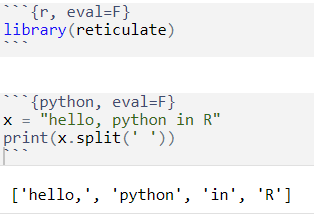
\includegraphics[width=2.60417in,height=\textheight]{images/02/lecticulate.png}

\hypertarget{markdown-uxbb38uxbc95}{%
\section{Markdown 문법}\label{markdown-uxbb38uxbc95}}

마크다운은 plain text 기반의 마크업 언어로서 마크업 언어는 태그 등을 이용해서 문서의 데이터 구조를 명시하는데 이러한 태그를 사용하는 방법 체계를 마크업 언어라고 합니다. 가장 대표적으로 html 이 있습니다.

\begin{verbatim}
    <html>
      <head>
        <title> Hello HTML </title>
      </head>
      <body>
      Hello markup world!
      </body>
    </html>
\end{verbatim}

마크다운도 몇 가지 태그를 이용해서 문서의 구조를 정의하고 있으며 상세한 내용은 \href{https://rmarkdown.rstudio.com/authoring_pandoc_markdown.html}{Pandoc 마크다운 문서}를 참고하시기 바랍니다. 마크다운언어의 철학은 쉽게 읽고 쓸 수 있는 문서입니다. plain text 기반으로 작성되어 쓰기 쉬우며 (아직도 사람들이 메모장 많이 사용하는 이유와 같습니다) 태그가 포함되어 있어도 읽는데 어려움이 없습니다. 위 html 언어와 아래 markdown 파일의 예들을 보시면 그 차이를 어렵지 않게 이해할 수 있습니다.

마크다운에서는 Enter를 한 번 입력해서 줄바꿈이 되지 않습니다. \texttt{\textless{}br\textgreater{}} 또는 문장 마지막에 공백을 두 개 입력하면 되겠습니다.

\begin{verbatim}
이 문장은 줄바꿈이 
되지 않습니다
\end{verbatim}

이 문장은 줄바꿈이
되지 않습니다

\begin{verbatim}
이 분장은 줄바꿈이<br>
됩니다
\end{verbatim}

이 분장은 줄바꿈이
됩니다

마크다운 테그를 몇 가지 살펴보면 먼저 \# 을 붙여서 만드는 header 가 있습니다.

\begin{verbatim}
# A level-one header
## A level-two header
### A level-three header

# A level-one header {#l1-1}
## A level-two header {#l2-1}
### A level-three header {#l3-1}

# A level-one header {#l1-2}
## A level-two header {#l2-2}
### A level-three header {#l3-2}
\end{verbatim}

Block quotations

\begin{quote}
This is block quote. This paragraph has two lines
\end{quote}

\begin{verbatim}
> This is block quote. This paragraph has two lines
\end{verbatim}

\begin{quote}
This is a block quote.

\begin{quote}
A block quote within a block quote.
\end{quote}
\end{quote}

\begin{verbatim}
> This is a block quote.
>
> > A block quote within a block quote.
\end{verbatim}

\emph{Italic}

\begin{verbatim}
*Italic*
\end{verbatim}

\textbf{Bold}

\begin{verbatim}
**Bold**
\end{verbatim}

\href{https://www.naver.com/}{Naver link}

\begin{verbatim}
[Naver link](https://www.naver.com/)
\end{verbatim}

이미지를 직접 삽입하고 가운데 정렬합니다.

\begin{figure}
\centering
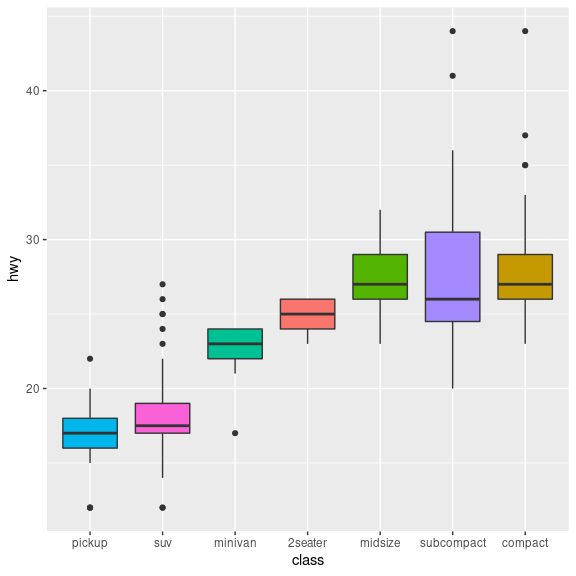
\includegraphics[width=2.08333in,height=\textheight]{images/rmarkdown/000002.png}
\caption{자동차 모델에 따른 고속도로 연비 분포}
\end{figure}

\begin{verbatim}
<center>
![자동차 모델에 따른 고속도로 연비 분포](images/rmarkdown/000002.png){width="200"}
</center>
\end{verbatim}

\begin{enumerate}
\def\labelenumi{\arabic{enumi}.}
\tightlist
\item
  첫 번째
\item
  두 번째
\item
  세 번째
\end{enumerate}

\begin{itemize}
\tightlist
\item
  아이템 1
\item
  아이템 2
\item
  아이템 3

  \begin{itemize}
  \tightlist
  \item
    아이템 3-1
  \item
    아이템 3-2
  \end{itemize}
\end{itemize}

\begin{verbatim}
1.  첫 번째
2.  두 번째
3.  세 번째

-   아이템 1
-   아이템 2
-   아이템 3
    -   아이템 3-1
    -   아이템 3-2
\end{verbatim}

참고로 소스코드 그대로 표현하기 위해서는 \texttt{\textasciitilde{}\textasciitilde{}\textasciitilde{}} 를 사용합니다.

\hypertarget{uxc2a4uxd0c0uxc77c}{%
\section{스타일}\label{uxc2a4uxd0c0uxc77c}}

아래와 같이 코드청크를 이용해서 css 코드를 삽입하고 해당되는 class 또는 id에 해당하는 내용에 스타일을 적용할 수 있습니다.

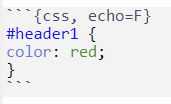
\includegraphics[width=1.5625in,height=\textheight]{images/02/style.png}

\leavevmode\vadjust pre{\hypertarget{header1}{}}%
소스코드

\begin{verbatim}
<div id='header1'>
소스코드 
</div>
\end{verbatim}

\hypertarget{uxd14cuxc774uxbe14}{%
\section{테이블}\label{uxd14cuxc774uxbe14}}

\texttt{kable} 함수를 이용하여 Rmarkdown 문서에 포함되는 표를 원하는 방향으로 작성할 수 있습니다. \texttt{mtcars}는 데이터프레임 형식의 데이터입니다.

\begin{Shaded}
\begin{Highlighting}[]
\NormalTok{knitr}\SpecialCharTok{::}\FunctionTok{kable}\NormalTok{(}
\NormalTok{  mtcars[}\DecValTok{1}\SpecialCharTok{:}\DecValTok{5}\NormalTok{, ], }
  \AttributeTok{caption =} \StringTok{"A knitr kable."}
\NormalTok{)}
\end{Highlighting}
\end{Shaded}

\begin{table}

\caption{\label{tab:unnamed-chunk-8}A knitr kable.}
\centering
\begin{tabular}[t]{l|r|r|r|r|r|r|r|r|r|r|r}
\hline
  & mpg & cyl & disp & hp & drat & wt & qsec & vs & am & gear & carb\\
\hline
Mazda RX4 & 21.0 & 6 & 160 & 110 & 3.90 & 2.620 & 16.46 & 0 & 1 & 4 & 4\\
\hline
Mazda RX4 Wag & 21.0 & 6 & 160 & 110 & 3.90 & 2.875 & 17.02 & 0 & 1 & 4 & 4\\
\hline
Datsun 710 & 22.8 & 4 & 108 & 93 & 3.85 & 2.320 & 18.61 & 1 & 1 & 4 & 1\\
\hline
Hornet 4 Drive & 21.4 & 6 & 258 & 110 & 3.08 & 3.215 & 19.44 & 1 & 0 & 3 & 1\\
\hline
Hornet Sportabout & 18.7 & 8 & 360 & 175 & 3.15 & 3.440 & 17.02 & 0 & 0 & 3 & 2\\
\hline
\end{tabular}
\end{table}

\hypertarget{yaml-uxd5e4uxb354}{%
\section{YAML 헤더}\label{yaml-uxd5e4uxb354}}

Rmarkdown 파일에서 YAML의 가장 중요한 기능은 output 포멧을 지정하는 것이며 title, author, date, 등을 설정할수도 있습니다.

\begin{verbatim}
---
layout: page
title: "R프로그래밍"
subtitle: "Rmarkdown 활용법"
output:
  html_document:
    css: style.css
    includes:
      in_header: header.html
      after_body: footer.html
    theme: default
    toc: yes
    toc_float: true
    highlight: tango
    code_folding: show
    number_sections: TRUE
mainfont: NanumGothic
---
\end{verbatim}

\hypertarget{output-format}{%
\section{Output format}\label{output-format}}

주요 문서 포멧으로 다음과 같은 몇 가지가 있습니다. 상세한 내용은 \href{https://rmarkdown.rstudio.com/lesson-9.html}{Rmarkdown output format}을 참고하시기 바랍니다.

\begin{itemize}
\tightlist
\item
  html\_document - HTML document w/ Bootstrap CSS
\item
  pdf\_document - PDF document (via LaTeX template)
\item
  word\_document - Microsoft Word document (docx)
\item
  ioslides\_presentation - HTML presentation with ioslides
\item
  beamer\_presentation - PDF presentation with LaTeX Beamer
\item
  powerpoint\_presentation: PowerPoint presentation
\end{itemize}

\textbf{Exercises}

``KRIBBR2022-Lecture2'' 라는 이름의 다음과 같은 형태의 Rmarkdown 문서를 만들고 이 번 강의의 실습 코드 및 설명, 질문, 코멘트 등을 적어 보시기 바랍니다.

\begin{center}\rule{0.5\linewidth}{0.5pt}\end{center}

이 저작물은 크리에이티브 커먼즈 저작자표시-비영리-변경금지 4.0 국제 라이선스에 따라 이용할 수 있습니다.

\hypertarget{r-programming}{%
\chapter{R programming}\label{r-programming}}

\hypertarget{console-calculator}{%
\section{Console calculator}\label{console-calculator}}

콘솔에서 바로 계산을 수행할 수 있습니다. 참고로 이전에 수행한 명령은 콘솔에 커서가 있는 상태에서 위 아래 화살표를 누르면 볼 수 있고 엔터를 눌러 재사용 할 수 있습니다. \texttt{;}을 사용하면 두 개의 명령을 동시에 수행할 수 있습니다.

\[ 2 + 2 \]
\[ ((2 - 1)^2 + (1 - 3)^2)^{1/2} \]

\begin{Shaded}
\begin{Highlighting}[]
\DecValTok{2} \SpecialCharTok{+} \DecValTok{2}
\NormalTok{((}\DecValTok{2}\NormalTok{ – }\DecValTok{1}\NormalTok{)}\SpecialCharTok{\^{}}\DecValTok{2} \SpecialCharTok{+}\NormalTok{ (}\DecValTok{1}\NormalTok{ – }\DecValTok{3}\NormalTok{)}\SpecialCharTok{\^{}}\DecValTok{2}\NormalTok{ )}\SpecialCharTok{\^{}}\NormalTok{(}\DecValTok{1}\SpecialCharTok{/}\DecValTok{2}\NormalTok{)}
\DecValTok{2} \SpecialCharTok{+} \DecValTok{2}\NormalTok{; }\DecValTok{2} \SpecialCharTok{{-}} \DecValTok{2}
\end{Highlighting}
\end{Shaded}

\textbf{Exercises}

다음 공식들을 계산하는 R 코드를 작성하시오

\[ \sqrt{(4+3)(2+1)} \]

\[ 2^3 + 3^2 \]

\[ \frac{0.25 - 0.2}{\sqrt{0.2 (1-0.2)/100}}\]

\hypertarget{what-is-a-programming-language}{%
\section{What is a programming language}\label{what-is-a-programming-language}}

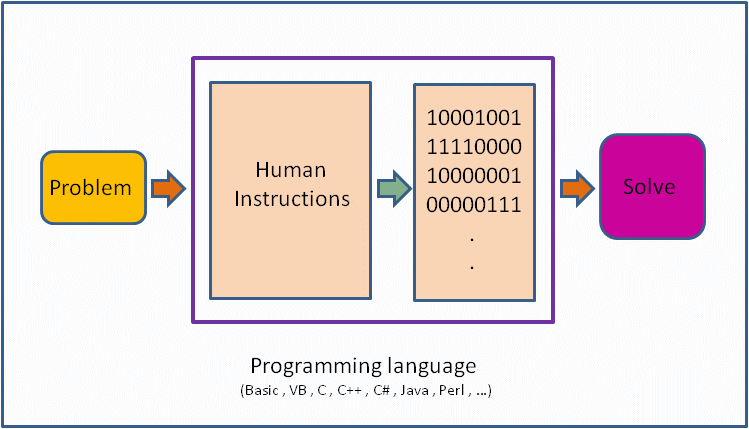
\includegraphics[width=4.16667in,height=\textheight]{images/01/24.PNG}

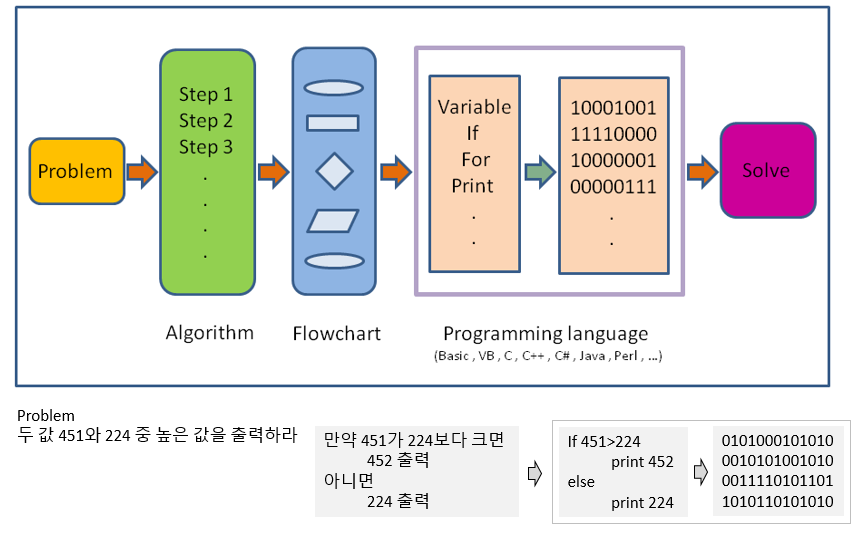
\includegraphics[width=4.375in,height=\textheight]{images/01/25.PNG}

R은 programming language로서 다른 프로그래밍 언어와 같이 몇 가지 공통적 개념을 가집니다 (\texttt{변수}, \texttt{자료형}, \texttt{함수}, \texttt{조건문}, \texttt{반복문})

\hypertarget{terminology}{%
\subsection{Terminology}\label{terminology}}

\begin{itemize}
\tightlist
\item
  Session: R 언어 실행 환경
\item
  Console: 명령어 입력하는 창
\item
  Code: R 프로그래밍 변수/제어문 모음
\item
  Object: 변수, 함수 등 프로그래밍에서 사용되는 모든 객체 (Data structure)

  \begin{itemize}
  \tightlist
  \item
    array: 1D, 2D, 3D, \ldots{} 형태 값들의 모임
  \item
    vector: 1차원 형태 값들의 모임 combine function \texttt{c()} EX: c(6, 11, 13, 31, 90, 92)
  \item
    matrix: 2차원 형태 값들의 모임 (같은 타입 값으로 구성)
  \item
    data frame: 2차원 형태 값들의 모임 (다른 타입 값 구성 가능)
  \item
    list: vector, matrix, data.frame 및 list 등 다양한 객체를 원소로 가집
  \end{itemize}
\item
  function: 특정 기능 수행, {[}함수이름, 입력값 (arguments), 출력값 (return){]} 으로 구성
\item
  Data (value): 값 - 자료형 (Data type)

  \begin{itemize}
  \tightlist
  \item
    Integers
  \item
    doubles/numerics
  \item
    logicals
  \item
    characters
  \item
    factor: 범주형
  \end{itemize}
\item
  Conditionals (조건, 제어):

  \begin{itemize}
  \tightlist
  \item
    \texttt{if}, \texttt{==}, \texttt{\&} (AND), \texttt{\textbar{}} (OR) Ex: \texttt{(2\ +\ 1\ ==\ 3)\ \&\ (2\ +\ 1\ ==\ 4)}
  \item
    \texttt{for}, \texttt{while}: 반복 수
  \end{itemize}
\end{itemize}

\hypertarget{data-and-variables}{%
\section{Data and variables}\label{data-and-variables}}

\hypertarget{data}{%
\subsection{Data}\label{data}}

일반적으로 데이터의 의미는 사실을 나타내는 수치입니다.

\begin{itemize}
\tightlist
\item
  맥도너 정보경제학 (1963)

  \begin{itemize}
  \tightlist
  \item
    지혜 (wisdom) : 패턴화된 지식
  \item
    지식 (knowledge) : 가치있는 정보
  \item
    정보 (information) : 의미있는 데이터
  \item
    데이터 (data) : 단순한 사실의 나열
  \end{itemize}
\end{itemize}

\begin{Shaded}
\begin{Highlighting}[]
\FunctionTok{library}\NormalTok{(UsingR)}
\NormalTok{exec.pay}
\NormalTok{?exec.pay}
\end{Highlighting}
\end{Shaded}

데이터는 속성에 따라서 다음과 같이 분류할 수 있습니다.

\begin{itemize}
\tightlist
\item
  범주형 - 질적 데이터, 숫자로 나타낼 수 있으나 의미 없음

  \begin{itemize}
  \tightlist
  \item
    명목형 (Nominal) - 사람 이름
  \item
    순서형 (Ordinal) -- 달리기 도착 순서
  \end{itemize}
\item
  수치형 - 숫자로 나타내며 데이터 속성을 그대로 지님님

  \begin{itemize}
  \tightlist
  \item
    구간형 (Interval) -- 선수1, 선수2 종점통과 시간
  \item
    비율형 (Ratio) -- 출발시간 기준 종점 통과 시간
  \end{itemize}
\end{itemize}

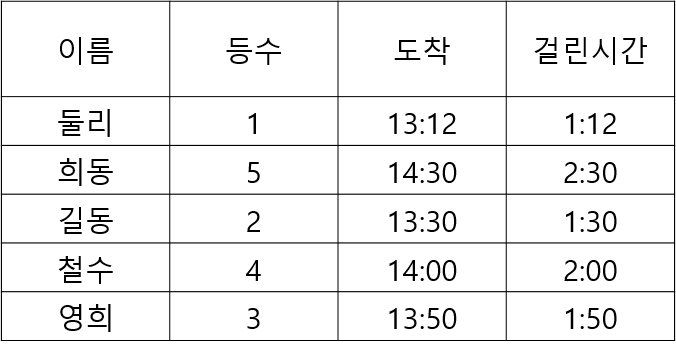
\includegraphics[width=3.125in,height=\textheight]{images/02/01.png}

\begin{itemize}
\tightlist
\item
  Data type in R

  \begin{itemize}
  \tightlist
  \item
    Numeric (수치형)

    \begin{itemize}
    \tightlist
    \item
      Discrete (이산형) data - 카운트, 횟수
    \item
      Continuous (연속형) data - 키, 몸무게, Cannot be shared
    \item
      Date and time
    \end{itemize}
  \item
    Factors (범주형)

    \begin{itemize}
    \tightlist
    \item
      Categories to group the data
    \item
      Character data - Identifiers (범주형)
    \end{itemize}
  \end{itemize}
\end{itemize}

\hypertarget{variables}{%
\subsection{Variables}\label{variables}}

변수는 데이터를 저장하는 공간으로 이해할 수 있습니다.

\begin{itemize}
\tightlist
\item
  Assignment operator ( \texttt{\textless{}-} OR \texttt{=} )

  \begin{itemize}
  \tightlist
  \item
    Valid object name \texttt{\textless{}-} value
  \item
    단축키: \texttt{Alt\ +\ -} (the minus sign)
  \end{itemize}
\item
  내장 변수 Built-in variables
\end{itemize}

\begin{Shaded}
\begin{Highlighting}[]
\NormalTok{x }\OtherTok{\textless{}{-}} \DecValTok{2}
\NormalTok{y }\OtherTok{\textless{}{-}}\NormalTok{ x}\SpecialCharTok{\^{}}\DecValTok{2}\NormalTok{ – }\DecValTok{2}\SpecialCharTok{*}\NormalTok{x }\SpecialCharTok{+} \DecValTok{1}
\NormalTok{y}
\NormalTok{x }\OtherTok{\textless{}{-}} \StringTok{"two"}  
\NormalTok{some\_data }\OtherTok{\textless{}{-}} \FloatTok{9.8}
\NormalTok{pi}
\end{Highlighting}
\end{Shaded}

\begin{itemize}
\tightlist
\item
  변수이름 작명법

  \begin{itemize}
  \tightlist
  \item
    Characters (letters), numbers, ``\_'', ``.''
  \item
    A and a are different symbols
  \item
    Names are effectively unlimited in length
  \end{itemize}
\end{itemize}

\begin{Shaded}
\begin{Highlighting}[]
\NormalTok{i\_use\_snake\_case }\OtherTok{\textless{}{-}} \DecValTok{1}
\NormalTok{otherPeopleUseCamelCase }\OtherTok{\textless{}{-}} \DecValTok{2}
\NormalTok{some.people.use.periods }\OtherTok{\textless{}{-}} \DecValTok{3}
\NormalTok{And\_aFew.People\_RENOUNCEconvention }\OtherTok{\textless{}{-}} \DecValTok{4}
\end{Highlighting}
\end{Shaded}

\hypertarget{object-data-structure}{%
\section{Object (Data structure)}\label{object-data-structure}}

변수, 함수 등 프로그래밍에서 사용되는 모든 개체를 말합니다.

\hypertarget{vector}{%
\subsection{vector}\label{vector}}

\texttt{vector}는 R의 기본 데이터 구조입니다. numeric vector, logical vector, character vector 등 저장되는 값의 타입에 따라 크게 세가지로 나눌 수 있습니다. \texttt{class()} 함수를 이용해서 값의 타입을 알아낼 수 있습니다. Combine function인 \texttt{c()}를 활용하여 만들며 값을 순차적으로 붙여갈 수 있습니다. 다음과 같은 Univariate (단변량, Single variable)을 표현할 때 사용됩니다.

\[ x_1, x_2, ..., x_n \]

\begin{Shaded}
\begin{Highlighting}[]
\NormalTok{x }\OtherTok{\textless{}{-}} \FunctionTok{c}\NormalTok{(}\FloatTok{10.4}\NormalTok{, }\FloatTok{5.6}\NormalTok{, }\FloatTok{3.1}\NormalTok{, }\FloatTok{6.4}\NormalTok{, }\FloatTok{21.7}\NormalTok{) }
\FunctionTok{class}\NormalTok{(x)}
\NormalTok{y }\OtherTok{\textless{}{-}} \FunctionTok{c}\NormalTok{(}\StringTok{"X1"}\NormalTok{, }\StringTok{"Y2"}\NormalTok{,  }\StringTok{"X3"}\NormalTok{,  }\StringTok{"Y4"}\NormalTok{)}
\FunctionTok{class}\NormalTok{(y)}
\NormalTok{z }\OtherTok{\textless{}{-}} \FunctionTok{c}\NormalTok{(T, F, F, T)}
\FunctionTok{class}\NormalTok{(z)}
\end{Highlighting}
\end{Shaded}

\hypertarget{numeric}{%
\subsubsection{numeric}\label{numeric}}

numeric 형식의 벡터는 다음과 같은 다양한 편의 함수들을 사용해서 만들수 있습니다.

\begin{Shaded}
\begin{Highlighting}[]
\DecValTok{1}\SpecialCharTok{:}\DecValTok{5}
\FunctionTok{seq}\NormalTok{(}\DecValTok{1}\NormalTok{,}\DecValTok{5}\NormalTok{, }\AttributeTok{by=}\DecValTok{1}\NormalTok{)}
\FunctionTok{seq}\NormalTok{(}\DecValTok{0}\NormalTok{, }\DecValTok{100}\NormalTok{, }\AttributeTok{by=}\DecValTok{10}\NormalTok{)}
\FunctionTok{seq}\NormalTok{(}\DecValTok{0}\NormalTok{, }\DecValTok{100}\NormalTok{, }\AttributeTok{length.out=}\DecValTok{11}\NormalTok{)}
\NormalTok{?seq}

\FunctionTok{rep}\NormalTok{(}\DecValTok{5}\NormalTok{, }\AttributeTok{times=}\DecValTok{10}\NormalTok{)}
\FunctionTok{rep}\NormalTok{(}\DecValTok{1}\SpecialCharTok{:}\DecValTok{3}\NormalTok{, }\AttributeTok{times=}\DecValTok{4}\NormalTok{)}
\FunctionTok{rep}\NormalTok{(}\DecValTok{1}\SpecialCharTok{:}\DecValTok{3}\NormalTok{, }\AttributeTok{each=}\DecValTok{3}\NormalTok{)}
\end{Highlighting}
\end{Shaded}

\textbf{Exercises}

odds라는 이름의 변수에 1부터 100까지의 홀수만을 저장하시오 (\texttt{seq()} 함수 사용)

인덱싱은 배열형 (vector, matrix 등) 데이터의 일부 데이터를 참조할 때 사용하는 방법입니다. \texttt{{[}}와 \texttt{{]}}를 사용하며 위치를 나타내는 수로 참조합니다.

\begin{Shaded}
\begin{Highlighting}[]
\NormalTok{x[}\DecValTok{1}\NormalTok{]}
\NormalTok{x[}\DecValTok{1}\SpecialCharTok{:}\DecValTok{3}\NormalTok{]}
\NormalTok{i }\OtherTok{\textless{}{-}} \DecValTok{1}\SpecialCharTok{:}\DecValTok{3}
\NormalTok{x[i]}
\NormalTok{x[}\FunctionTok{c}\NormalTok{(}\DecValTok{1}\NormalTok{,}\DecValTok{2}\NormalTok{,}\DecValTok{4}\NormalTok{)]}
\NormalTok{y[}\DecValTok{3}\NormalTok{]}
\end{Highlighting}
\end{Shaded}

또한 해당 위치의 이름으로 참조하기도 합니다.

\begin{Shaded}
\begin{Highlighting}[]
\FunctionTok{head}\NormalTok{(precip)}
\NormalTok{precip[}\DecValTok{1}\NormalTok{]}
\NormalTok{precip[}\DecValTok{2}\SpecialCharTok{:}\DecValTok{10}\NormalTok{]}
\NormalTok{precip[}\FunctionTok{c}\NormalTok{(}\DecValTok{1}\NormalTok{,}\DecValTok{3}\NormalTok{,}\DecValTok{5}\NormalTok{)]}
\NormalTok{precip[}\SpecialCharTok{{-}}\DecValTok{1}\NormalTok{]}
\NormalTok{precip[}\StringTok{"Seattle Tacoma"}\NormalTok{]}
\NormalTok{precip[}\FunctionTok{c}\NormalTok{(}\StringTok{"Seattle Tacoma"}\NormalTok{, }\StringTok{"Portland"}\NormalTok{)]}
\NormalTok{precip[}\DecValTok{2}\NormalTok{] }\OtherTok{\textless{}{-}} \DecValTok{10}
\end{Highlighting}
\end{Shaded}

참고로 vector 들은 다음과 같은 builtin 함수들을 사용해서 해당 변수의 attribute를 알아낼 수 있습니다. attribute에는 원소 이름, 타입, 길이 등 vector형 변수가 가질 수 있는 특성을 말합니다.

\begin{Shaded}
\begin{Highlighting}[]
\FunctionTok{head}\NormalTok{(precip)}
\FunctionTok{class}\NormalTok{(precip)}
\FunctionTok{length}\NormalTok{(precip)}
\FunctionTok{names}\NormalTok{(precip)}

\NormalTok{test\_scores }\OtherTok{\textless{}{-}} \FunctionTok{c}\NormalTok{(}\DecValTok{100}\NormalTok{, }\DecValTok{90}\NormalTok{, }\DecValTok{80}\NormalTok{)}
\FunctionTok{names}\NormalTok{(test\_scores) }\OtherTok{\textless{}{-}} \FunctionTok{c}\NormalTok{(}\StringTok{"Alice"}\NormalTok{, }\StringTok{"Bob"}\NormalTok{, }\StringTok{"Shirley"}\NormalTok{)}
\NormalTok{test\_scores}
\end{Highlighting}
\end{Shaded}

\hypertarget{logical}{%
\subsubsection{logical}\label{logical}}

Logical 벡터는 \texttt{True} 또는 \texttt{False}를 원소로 갖는 벡터 입니다. 앞글자가 대분자로 시작하는 것을 기억하시고 \texttt{T} 또는 \texttt{F}와 같이 한 문자로 표현할 수도 있습니다. 특정 조건에 대한 판단 결과를 반환할 경우에도 논리값을 사용합니다. 이 경우 조건을 판단 후 인덱싱 방법으로 (\texttt{which}, \texttt{any}, \texttt{all} 등 사용) 해당 값들을 뽑아내기도 합니다. 또한 활용이 많은 \texttt{sample} 함수의 사용법을 익혀둡니다.

\begin{Shaded}
\begin{Highlighting}[]
\NormalTok{x }\OtherTok{\textless{}{-}} \DecValTok{1}\SpecialCharTok{:}\DecValTok{20}
\NormalTok{x }\SpecialCharTok{\textgreater{}} \DecValTok{13}
\NormalTok{temp }\OtherTok{\textless{}{-}}\NormalTok{ x }\SpecialCharTok{\textgreater{}} \DecValTok{13}
\FunctionTok{class}\NormalTok{(temp)}

\NormalTok{ages }\OtherTok{\textless{}{-}} \FunctionTok{c}\NormalTok{(}\DecValTok{66}\NormalTok{, }\DecValTok{57}\NormalTok{, }\DecValTok{60}\NormalTok{, }\DecValTok{41}\NormalTok{,  }\DecValTok{6}\NormalTok{, }\DecValTok{85}\NormalTok{, }\DecValTok{48}\NormalTok{, }\DecValTok{34}\NormalTok{, }\DecValTok{61}\NormalTok{, }\DecValTok{12}\NormalTok{)}
\NormalTok{ages }\SpecialCharTok{\textless{}} \DecValTok{30}
\FunctionTok{which}\NormalTok{(ages }\SpecialCharTok{\textless{}} \DecValTok{30}\NormalTok{)}
\NormalTok{i }\OtherTok{\textless{}{-}} \FunctionTok{which}\NormalTok{(ages }\SpecialCharTok{\textless{}} \DecValTok{30}\NormalTok{)}
\NormalTok{ages[i]}
\FunctionTok{any}\NormalTok{(ages }\SpecialCharTok{\textless{}} \DecValTok{30}\NormalTok{)}
\FunctionTok{all}\NormalTok{(ages }\SpecialCharTok{\textless{}} \DecValTok{30}\NormalTok{)}

\NormalTok{random\_number }\OtherTok{\textless{}{-}} \FunctionTok{sample}\NormalTok{(}\FunctionTok{c}\NormalTok{(}\DecValTok{1}\SpecialCharTok{:}\DecValTok{10}\NormalTok{), }\DecValTok{2}\NormalTok{)}
\end{Highlighting}
\end{Shaded}

\textbf{Exercises}
1. 1부터 100까지의 수를 evens이라는 이름의 변수에 저장하고 이 중 짝수만을 뽑아내서 출력하시오 (\texttt{which()}함수 사용)

\begin{enumerate}
\def\labelenumi{\arabic{enumi}.}
\setcounter{enumi}{1}
\item
  \texttt{sample} 함수를 사용하여 앞서 odds와 evens 변수에서 랜덤하게 1개씩의 샘플을 뽑아서 \texttt{mynumbers}에 저장하시오
\item
  어떤 짝수가 뽑혔는지 찾아서 출력하시오 (\texttt{which}와 인덱싱 사용)
\end{enumerate}

\hypertarget{character}{%
\subsubsection{character}\label{character}}

Character(문자형) 벡터의 경우 문자열을 다루는데 자주 쓰이는 \texttt{paste()} 함수의 사용법을 알아두면 편리합니다. \texttt{paste()} 함수는 서로 다른 문자열을 붙이는데 주로 사용됩니다. 참고로 문자열을 나누는 함수는 \texttt{strsplit()} 입니다. \texttt{paste()}에서 붙이는 문자 사이에 들어가는 문자를 지정하는 파라메터는 \texttt{sep} 이고 \texttt{strsplit()}함수에서 자르는 기준이 되는 문자는\texttt{split} 파라미터로 지정해 줍니다 (\texttt{?split} 또는 \texttt{?paste} 확인).

\begin{Shaded}
\begin{Highlighting}[]
\FunctionTok{paste}\NormalTok{(}\StringTok{"X"}\NormalTok{, }\StringTok{"Y"}\NormalTok{, }\StringTok{"Z"}\NormalTok{, }\AttributeTok{sep=}\StringTok{"\_"}\NormalTok{)}
\FunctionTok{paste}\NormalTok{(}\FunctionTok{c}\NormalTok{(}\StringTok{"Four"}\NormalTok{,}\StringTok{"The"}\NormalTok{), }\FunctionTok{c}\NormalTok{(}\StringTok{"Score"}\NormalTok{,}\StringTok{"quick"}\NormalTok{), }\FunctionTok{c}\NormalTok{(}\StringTok{"and"}\NormalTok{,}\StringTok{"fox"}\NormalTok{), }\AttributeTok{sep=}\StringTok{"\_"}\NormalTok{)}
\FunctionTok{paste}\NormalTok{(}\StringTok{"X"}\NormalTok{, }\DecValTok{1}\SpecialCharTok{:}\DecValTok{5}\NormalTok{, }\AttributeTok{sep=}\StringTok{""}\NormalTok{)}
\FunctionTok{paste}\NormalTok{(}\FunctionTok{c}\NormalTok{(}\StringTok{"X"}\NormalTok{,}\StringTok{"Y"}\NormalTok{), }\DecValTok{1}\SpecialCharTok{:}\DecValTok{10}\NormalTok{, }\AttributeTok{sep=}\StringTok{""}\NormalTok{)}

\NormalTok{x }\OtherTok{\textless{}{-}} \FunctionTok{c}\NormalTok{(}\StringTok{"X1"}\NormalTok{, }\StringTok{"Y2"}\NormalTok{, }\StringTok{"X3"}\NormalTok{, }\StringTok{"Y4"}\NormalTok{, }\StringTok{"X5"}\NormalTok{)}
\FunctionTok{paste}\NormalTok{(x[}\DecValTok{1}\NormalTok{], x[}\DecValTok{2}\NormalTok{])}
\FunctionTok{paste}\NormalTok{(x[}\DecValTok{1}\NormalTok{], x[}\DecValTok{2}\NormalTok{], }\AttributeTok{sep=}\StringTok{""}\NormalTok{)}
\FunctionTok{paste}\NormalTok{(x, }\AttributeTok{collapse=}\StringTok{"\_"}\NormalTok{)}

\FunctionTok{strsplit}\NormalTok{(}\StringTok{"XYZ"}\NormalTok{, }\AttributeTok{split=}\StringTok{""}\NormalTok{)}
\FunctionTok{sort}\NormalTok{(}\FunctionTok{c}\NormalTok{(}\StringTok{"B"}\NormalTok{, }\StringTok{"C"}\NormalTok{, }\StringTok{"A"}\NormalTok{, }\StringTok{"D"}\NormalTok{))}
\end{Highlighting}
\end{Shaded}

\textbf{Exercises}

\begin{enumerate}
\def\labelenumi{\arabic{enumi}.}
\item
  \texttt{m}이라는 변수에 ``Capital of South Korea is Seoul'' 문자열을 저장하고 ``Capital of South Korea''를 따로 뽑아내 \texttt{m2}에 저장하시오 (\texttt{substr()} 사용)
\item
  \texttt{LETTERS} 내장함수에서 랜덤하게 10개의 문자를 뽑아내 myletters 변수에 저장하고 이들을 연결하여 (\texttt{paste} 사용) 하나의 문장(String)을 만드시오
\item
  myletters 변수의 문자들을 알파벳 순서대로 정렬하고 (\texttt{sort} 사용) 이들을 연결하여 하나의 문장 (String)을 만드시오
\end{enumerate}

\hypertarget{factor}{%
\subsubsection{factor}\label{factor}}

Factor형은 범주형데이터를 저장하기 위한 object 이며 R 언어에서 특별히 만들어져 사용되고 있습니다. \texttt{factor()} 함수를 이용해 생성하며 생성된 객체는 다음과 같이 \texttt{level}이라는 범주를 나타내는 특성값을 가지고 있습니다.

예를 들어 어린이 5명이 각각 빨강, 파랑, 노랑, 빨강, 파랑 색종이를 들고 있을때 색의 종류를 나타내는 값들은 빨강, 파랑, 노랑 입니다. 다섯 명의 아이들이 어떤 색의 색종이를 들고 있는지와는 상관없이 세 가지 범주의 값을 가지는 것 입니다.

\begin{Shaded}
\begin{Highlighting}[]
\NormalTok{x }\OtherTok{\textless{}{-}} \FunctionTok{c}\NormalTok{(}\StringTok{"Red"}\NormalTok{, }\StringTok{"Blue"}\NormalTok{, }\StringTok{"Yellow"}\NormalTok{, }\StringTok{"Red"}\NormalTok{, }\StringTok{"Blue"}\NormalTok{)}
\NormalTok{y }\OtherTok{\textless{}{-}} \FunctionTok{factor}\NormalTok{(x)}
\NormalTok{y}
\end{Highlighting}
\end{Shaded}

새로운 범주의 데이터를 추가할 경우 다음과 같이 해당되는 level을 먼저 추가하고 값을 저장해야 합니다.

\begin{Shaded}
\begin{Highlighting}[]
\FunctionTok{levels}\NormalTok{(y)}
\NormalTok{y[}\DecValTok{1}\NormalTok{] }\OtherTok{\textless{}{-}} \StringTok{"Gold"}
\NormalTok{y}

\FunctionTok{levels}\NormalTok{(y) }\OtherTok{\textless{}{-}} \FunctionTok{c}\NormalTok{(}\FunctionTok{levels}\NormalTok{(y), }\StringTok{"Gold"}\NormalTok{)}
\FunctionTok{levels}\NormalTok{(y)}
\NormalTok{y}
\NormalTok{y[}\DecValTok{1}\NormalTok{] }\OtherTok{\textless{}{-}} \StringTok{"Gold"}
\NormalTok{y}
\end{Highlighting}
\end{Shaded}

\texttt{factor}는 기본적으로 \texttt{level}에 표시된 순서가 위치 (정렬) 순서입니다. 이를 바꾸기 위해서는 다음과 같이 \texttt{levels} 함수를 이용해서 순서를 바꿀 수 있습니다.

\begin{Shaded}
\begin{Highlighting}[]
\FunctionTok{library}\NormalTok{(MASS)}
\FunctionTok{str}\NormalTok{(Cars93)}
\NormalTok{x }\OtherTok{\textless{}{-}}\NormalTok{ Cars93}\SpecialCharTok{$}\NormalTok{Origin}
\FunctionTok{plot}\NormalTok{(x)}
\FunctionTok{levels}\NormalTok{(x) }\OtherTok{\textless{}{-}} \FunctionTok{c}\NormalTok{(}\StringTok{"non{-}USA"}\NormalTok{, }\StringTok{"USA"}\NormalTok{)}
\FunctionTok{levels}\NormalTok{(x)}
\FunctionTok{plot}\NormalTok{(x)}
\end{Highlighting}
\end{Shaded}

\textbf{Exercises}

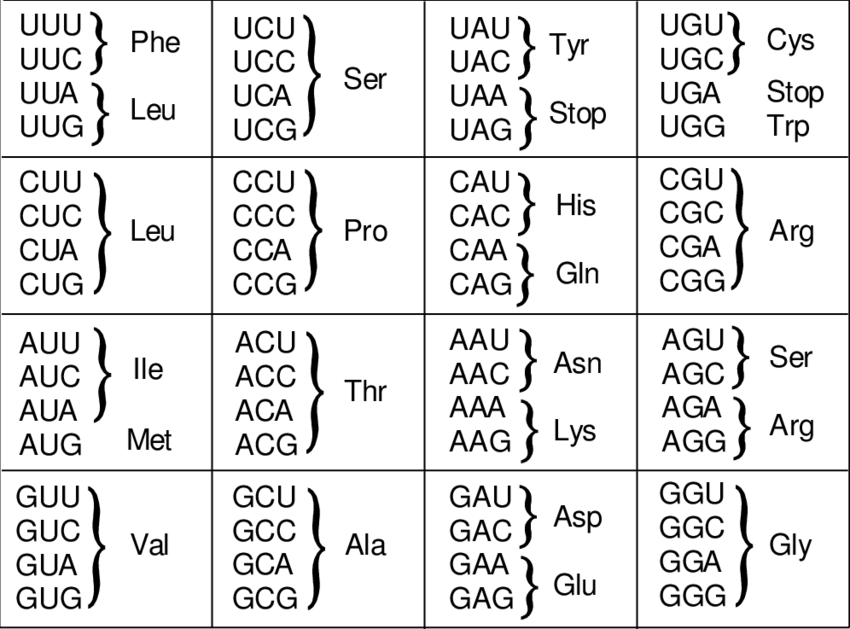
\includegraphics[width=3.64583in,height=\textheight]{images/03/codon_table.png}
1. 아미노산 Phe, Leu, Ser 를 값으로 갖는 범주형 변수 (factor)를 생성하시오
2. 각 아미노산과 해당 아미노산을 코딩하는 nucleotide triplets (codon)을 어떤 형태의 변수로 저장할 수 있을지 고민해 보시오

\hypertarget{missing-values}{%
\subsubsection{Missing values}\label{missing-values}}

특정 값이 ``Not available'' 이거나 ``Missing value'' 일 경우 벡터의 해당 원소 자리에 데이터의 이상을 알리기 위해 \texttt{NA}를 사용합니다. 따라서 일반적인 연산에서 \texttt{NA}가 포함되어 있는 경우 데이터의 불완전성을 알리기 위해 연산의 결과는 \texttt{NA}가 됩니다. \texttt{is.na()} 함수는 해당 변수에 \texttt{NA} 값이 있는지를 검사해주는 함수이며 R에는 이 외에도 다음과 같은 특수 값들이 사용되고 있습니다.

\begin{itemize}
\tightlist
\item
  NA: Not available, The value is missing
\item
  NULL: a reserved value
\item
  NaN: Not a number (0/0)
\item
  Inf: (1/0)
\end{itemize}

\begin{Shaded}
\begin{Highlighting}[]
\NormalTok{hip\_cost }\OtherTok{\textless{}{-}} \FunctionTok{c}\NormalTok{(}\DecValTok{10500}\NormalTok{, }\DecValTok{45000}\NormalTok{, }\DecValTok{74100}\NormalTok{, }\ConstantTok{NA}\NormalTok{, }\DecValTok{83500}\NormalTok{)}
\FunctionTok{sum}\NormalTok{(hip\_cost)}
\FunctionTok{sum}\NormalTok{(hip\_cost, }\AttributeTok{na.rm=}\ConstantTok{TRUE}\NormalTok{)}
\NormalTok{?sum}
\end{Highlighting}
\end{Shaded}

\hypertarget{useful-functions}{%
\subsubsection{Useful functions}\label{useful-functions}}

다음은 벡터형 변수와 같이 쓰이는 유용한 함수들입니다.

\begin{Shaded}
\begin{Highlighting}[]
\NormalTok{z }\OtherTok{\textless{}{-}} \FunctionTok{sample}\NormalTok{(}\DecValTok{1}\SpecialCharTok{:}\DecValTok{10}\NormalTok{, }\DecValTok{100}\NormalTok{, T)}
\FunctionTok{head}\NormalTok{(z)}
\FunctionTok{sort}\NormalTok{(z)}
\FunctionTok{order}\NormalTok{(z)}
\FunctionTok{table}\NormalTok{(z)}
\NormalTok{p }\OtherTok{\textless{}{-}}\NormalTok{ z}\SpecialCharTok{/}\FunctionTok{sum}\NormalTok{(z)}
\FunctionTok{round}\NormalTok{(p, }\AttributeTok{digits=}\DecValTok{1}\NormalTok{)}
\end{Highlighting}
\end{Shaded}

\texttt{is} 함수를 사용하여 데이터 타입이 사용자가 의도한 타입과 맞는지 검사할 수 있습니다. 콘솔창에서 \texttt{is.}를 타이핑한 후 잠시 기다리면 다양한 is 합수를 볼 수 있습니다.

\begin{Shaded}
\begin{Highlighting}[]
\FunctionTok{is.na}\NormalTok{(}\DecValTok{1}\NormalTok{)}
\FunctionTok{is.numeric}\NormalTok{(}\DecValTok{1}\NormalTok{)}
\FunctionTok{is.logical}\NormalTok{(}\ConstantTok{TRUE}\NormalTok{)}
\FunctionTok{is.data.frame}\NormalTok{(}\StringTok{"A"}\NormalTok{)}
\FunctionTok{is.character}\NormalTok{(}\StringTok{"A"}\NormalTok{)}
\end{Highlighting}
\end{Shaded}

\texttt{as} 함수는 데이터 타입을 변환해주는 함수입니다.

\begin{Shaded}
\begin{Highlighting}[]
\NormalTok{digits }\OtherTok{\textless{}{-}} \FunctionTok{runif}\NormalTok{(}\DecValTok{10}\NormalTok{)}\SpecialCharTok{*}\DecValTok{10}
\FunctionTok{class}\NormalTok{(digits)}
\NormalTok{digits\_int }\OtherTok{\textless{}{-}} \FunctionTok{as.integer}\NormalTok{(digits)}
\FunctionTok{class}\NormalTok{(digits\_int)}
\NormalTok{digits\_char }\OtherTok{\textless{}{-}} \FunctionTok{as.character}\NormalTok{(digits\_int)}
\FunctionTok{class}\NormalTok{(digits\_char)}
\NormalTok{digits\_num }\OtherTok{\textless{}{-}} \FunctionTok{as.numeric}\NormalTok{(digits\_char)}
\FunctionTok{class}\NormalTok{(digits\_num)}
\end{Highlighting}
\end{Shaded}

\hypertarget{matrix}{%
\subsection{matrix}\label{matrix}}

매트릭스는 2차원 행렬로 같은 형식의 데이터 값 (numberic, character, logical) 으로만 채워진 행렬을 말합니다. 메트릭스를 만드는 방법은 아래와 같으며 \texttt{nrow} 와 \texttt{ncol} 파라메터에 행과 열의 수를 넣고 각 셀에 들어갈 값은 가장 앞에 위치한 data 파라메터에 넣어 줍니다 (\texttt{?matrix}로 파라메터 이름 확인). 메트릭스 인덱싱은 메트릭스 안의 값을 저장하거나 참조할때 (빼올때) 사용하는 방법입니다. 메트릭스 변수이름 바로 뒤에 대괄호를 이용해서 제어를 하며 대괄호 안에 콤마로 구분된 앞쪽은 row, 뒷쪽은 column 인덱스를 나타냅니다.

\begin{Shaded}
\begin{Highlighting}[]
\NormalTok{mymat }\OtherTok{\textless{}{-}} \FunctionTok{matrix}\NormalTok{(}\DecValTok{0}\NormalTok{, }\AttributeTok{nrow=}\DecValTok{100}\NormalTok{, }\AttributeTok{ncol=}\DecValTok{3}\NormalTok{) }\CommentTok{\# 1}
\NormalTok{mymat[,}\DecValTok{1}\NormalTok{] }\OtherTok{\textless{}{-}} \DecValTok{1}\SpecialCharTok{:}\DecValTok{100} \CommentTok{\# 2}
\NormalTok{mymat[,}\DecValTok{2}\NormalTok{] }\OtherTok{\textless{}{-}} \FunctionTok{seq}\NormalTok{(}\DecValTok{1}\NormalTok{,}\DecValTok{200}\NormalTok{,}\DecValTok{2}\NormalTok{) }\CommentTok{\# 3}
\NormalTok{mymat[,}\DecValTok{3}\NormalTok{] }\OtherTok{\textless{}{-}} \FunctionTok{seq}\NormalTok{(}\DecValTok{2}\NormalTok{,}\DecValTok{200}\NormalTok{,}\DecValTok{2}\NormalTok{) }\CommentTok{\# 4}
\end{Highlighting}
\end{Shaded}

매트릭스의 row나 column에 이름이 주어져 있을 경우 이름을 따옴표(``)로 묶은 후 참조가 가능합니다. row나 column의 이름은 \texttt{rownames()} 또는 \texttt{colnames()}로 생성하거나 변경할 수 있습니다. row나 column의 개수는 \texttt{nrow()} 또는 \texttt{ncol()} 함수를 사용합니다.

\begin{Shaded}
\begin{Highlighting}[]
\FunctionTok{colnames}\NormalTok{(mymat)}
\FunctionTok{colnames}\NormalTok{(mymat) }\OtherTok{\textless{}{-}} \FunctionTok{c}\NormalTok{(}\StringTok{"A"}\NormalTok{, }\StringTok{"B"}\NormalTok{, }\StringTok{"C"}\NormalTok{)}
\FunctionTok{colnames}\NormalTok{(mymat)}
\FunctionTok{colnames}\NormalTok{(mymat)[}\DecValTok{2}\NormalTok{] }\OtherTok{\textless{}{-}} \StringTok{"D"}
\FunctionTok{colnames}\NormalTok{(mymat)}
\FunctionTok{rownames}\NormalTok{(mymat) }\OtherTok{\textless{}{-}} \FunctionTok{paste}\NormalTok{(}\StringTok{"No"}\NormalTok{, }\DecValTok{1}\SpecialCharTok{:}\FunctionTok{nrow}\NormalTok{(mymat), }\AttributeTok{sep=}\StringTok{""}\NormalTok{)}
\FunctionTok{rownames}\NormalTok{(mymat)}
\end{Highlighting}
\end{Shaded}

여러 row나 column을 참조할 경우 아래와 같이 combine 함수를 사용하여 묶어줘야 하며 스칼라값을 (임의의 숫자 하나) 더하거나 뺄 경우 vector / matrix 연산을 기본으로 수행합니다.

\begin{Shaded}
\begin{Highlighting}[]
\NormalTok{mymat[}\FunctionTok{c}\NormalTok{(}\DecValTok{2}\NormalTok{,}\DecValTok{3}\NormalTok{,}\DecValTok{4}\NormalTok{,}\DecValTok{5}\NormalTok{),}\DecValTok{2}\NormalTok{] }\CommentTok{\# 5}
\NormalTok{mymat}\DecValTok{{-}1} \CommentTok{\# 6}
\NormalTok{mysub }\OtherTok{\textless{}{-}}\NormalTok{ mymat[,}\DecValTok{2}\NormalTok{] }\SpecialCharTok{{-}}\NormalTok{ mymat[,}\DecValTok{1}\NormalTok{] }\CommentTok{\#7}
\FunctionTok{sum}\NormalTok{(mysub) }\CommentTok{\#8}
\FunctionTok{sum}\NormalTok{(mysub}\SpecialCharTok{\^{}}\DecValTok{2}\NormalTok{) }\CommentTok{\#8}
\end{Highlighting}
\end{Shaded}

\textbf{Exercises}

\begin{enumerate}
\def\labelenumi{\arabic{enumi}.}
\tightlist
\item
  score 라는 변수에 1부터 100까지 중 랜덤하게 선택된 20개의 수로 10 x 2 matrix를 만드시오 (\texttt{sample()} 사용)
\item
  score의 row 이름을 문자형으로 Name1, Name2, \ldots, Name10으로 지정하시오 (\texttt{paste()} 사용)
\item
  score의 column 이름을 문자형으로 math와 eng로 지정하시오
\item
  이 matrix의 첫번째 컬럼과 두 번째 컬럼의 수를 각각 더한 후 \texttt{total\_score}라는 변수에 저장하시오
\item
  \texttt{total\_score}의의 오름차순 순서를 나타내는 인덱스 (\texttt{order()}함수 사용)를 \texttt{o}라는 변수에 저장하시오
\item
  score를 \texttt{o}순서로 재배치하고 score\_ordered 변수에 저장하시오
\end{enumerate}

\hypertarget{data.frame}{%
\subsection{data.frame}\label{data.frame}}

데이터프레임은 형태는 매트릭스와 같으나 컬럼 하나가 하나의 vector형 변수로서 각 변수들이 다른 모드의 값을 저장할 수 있다는 차이가 있습니다. \texttt{\$} 기호를 이용하여 각 구성 변수를 참조할 수 있습니다. 컬럼 한 줄이 하나의 변수 이므로 새로운 변수도 컬럼 형태로 붙여 넣을 수 있습니다. 즉, 각 row는 샘플을 나타내고 각 column은 변수를 나타내며 각 변수들이 갖는 샘플의 개수 (row의 길이, vector 의 길이)는 같아야 합니다. R 기반의 데이터 분석에서는 가장 선호되는 데이터 타입이라고 볼 수 있습니다.

\begin{Shaded}
\begin{Highlighting}[]
\DocumentationTok{\#\# data.frame}
\NormalTok{ids }\OtherTok{\textless{}{-}} \DecValTok{1}\SpecialCharTok{:}\DecValTok{10}
\NormalTok{ids}
\NormalTok{idnames }\OtherTok{\textless{}{-}} \FunctionTok{paste}\NormalTok{(}\StringTok{"Name"}\NormalTok{, ids, }\AttributeTok{sep=}\StringTok{""}\NormalTok{)}
\NormalTok{idnames}
\NormalTok{students }\OtherTok{\textless{}{-}} \FunctionTok{data.frame}\NormalTok{(ids, idnames)}
\NormalTok{students}
\FunctionTok{class}\NormalTok{(students}\SpecialCharTok{$}\NormalTok{ids)}
\FunctionTok{class}\NormalTok{(students}\SpecialCharTok{$}\NormalTok{idnames)}
\NormalTok{students}\SpecialCharTok{$}\NormalTok{idnames}
\FunctionTok{str}\NormalTok{(students)}

\NormalTok{students }\OtherTok{\textless{}{-}} \FunctionTok{data.frame}\NormalTok{(ids, idnames, }\AttributeTok{stringsAsFactors =}\NormalTok{ F)}
\FunctionTok{class}\NormalTok{(students}\SpecialCharTok{$}\NormalTok{idnames)}
\NormalTok{students}\SpecialCharTok{$}\NormalTok{idnames}
\NormalTok{students[}\DecValTok{1}\NormalTok{,]}
\FunctionTok{str}\NormalTok{(students)}
\end{Highlighting}
\end{Shaded}

데이터프레임에서는 \texttt{\$}를 사용하여 변수 이름으로 인덱싱이 가능합니다.

\begin{Shaded}
\begin{Highlighting}[]
\DocumentationTok{\#\# data frame indexing }
\NormalTok{students}\SpecialCharTok{$}\NormalTok{ids}
\NormalTok{students[,}\DecValTok{1}\NormalTok{]}
\NormalTok{students[,}\StringTok{"ids"}\NormalTok{]}
\end{Highlighting}
\end{Shaded}

\textbf{Exercises}

\begin{enumerate}
\def\labelenumi{\arabic{enumi}.}
\tightlist
\item
  \texttt{math}라는 변수에 1부터 100까지 중 랜덤하게 선택된 10개의 수를 넣으시오
\item
  \texttt{eng}라는 변수에 1부터 100까지 중 랜덤하게 선택된 10개의 수를 넣으시오
\item
  \texttt{students}라는 변수에 문자형으로 Name1, Name2, \ldots, Name10으로 지정하시오 (\texttt{paste()} 사용)
\item
  \texttt{math}와 \texttt{eng}라는 벡터에 저장된 값들의 이름을 \texttt{students} 변수에 저장된 이름으로 지정하시오
\item
  \texttt{math}와 \texttt{eng} 벡터를 갖는 \texttt{score} 라는 \texttt{data.frame}을 만드시오
\item
  \texttt{math}와 \texttt{eng} 변수를 지우시오 (\texttt{rm()}사용)
\item
  \texttt{score} data frame의 \texttt{math}와 \texttt{eng}를 각각 더한 후 \texttt{total\_score}라는 변수에 저장 하시오
\end{enumerate}

\hypertarget{list}{%
\subsection{list}\label{list}}

리스트는 변수들의 모임이라는 점에서 데이터프레임과 같으나 구성 변수들의 길이가 모두 같아야 하는 데이터프레임과는 달리 다른 길이의 변수를 모아둘 수 있는 점이 다릅니다. 즉, R언어에서 두 변수를 담을 수 있는 데이터 타입은 \texttt{list}와 \texttt{data\ frame} 두 종류가 있는데 \texttt{list} 변수 타입은 \texttt{vector} 형태의 여러개의 element를 가질 수 있으며 각 \texttt{vector의} 길이가 모두 달라도 됩니다. list의 인덱싱에서 \texttt{{[}} \texttt{{]}}는 리스트를 반환하고 \texttt{{[}{[}} \texttt{{]}{]}}는 vector element들을 반환합니다.

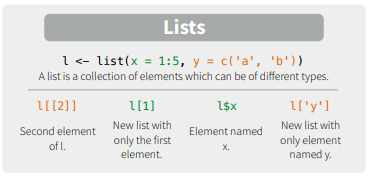
\includegraphics[width=3.125in,height=\textheight]{images/03/05.PNG}

\begin{Shaded}
\begin{Highlighting}[]
\DocumentationTok{\#\# list}
\NormalTok{parent\_names }\OtherTok{\textless{}{-}} \FunctionTok{c}\NormalTok{(}\StringTok{"Fred"}\NormalTok{, }\StringTok{"Mary"}\NormalTok{)}
\NormalTok{number\_of\_children }\OtherTok{\textless{}{-}} \DecValTok{2}
\NormalTok{child\_ages }\OtherTok{\textless{}{-}} \FunctionTok{c}\NormalTok{(}\DecValTok{4}\NormalTok{, }\DecValTok{7}\NormalTok{, }\DecValTok{9}\NormalTok{)}
\FunctionTok{data.frame}\NormalTok{(parent\_names, number\_of\_children, child\_ages)}
\NormalTok{lst }\OtherTok{\textless{}{-}} \FunctionTok{list}\NormalTok{(parent\_names, number\_of\_children, child\_ages)}
\NormalTok{lst[}\DecValTok{1}\NormalTok{]}
\NormalTok{lst[[}\DecValTok{1}\NormalTok{]]}
\FunctionTok{class}\NormalTok{(lst[}\DecValTok{1}\NormalTok{])}
\FunctionTok{class}\NormalTok{(lst[[}\DecValTok{1}\NormalTok{]])}
\NormalTok{lst[[}\DecValTok{1}\NormalTok{]][}\DecValTok{1}\NormalTok{]}
\NormalTok{lst[[}\DecValTok{1}\NormalTok{]][}\FunctionTok{c}\NormalTok{(}\DecValTok{1}\NormalTok{,}\DecValTok{2}\NormalTok{)]}
\end{Highlighting}
\end{Shaded}

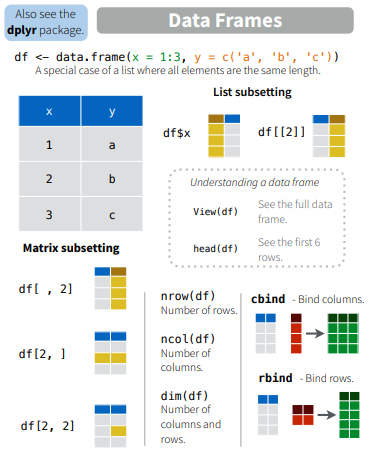
\includegraphics[width=2.60417in,height=\textheight]{images/03/06.PNG}

\textbf{Exercises}

\begin{enumerate}
\def\labelenumi{\arabic{enumi}.}
\item
  위 아미노산 예제에서 Phe, Leu, Ser 각각의 코돈을 원소로 갖는 세 개의 vector 변수들을 만들고 이를 \texttt{aalist} 라는 이름의 하나의 리스트 변수로 만드시오
\item
  \texttt{aalist} 리스트를 data.frame 형식의 \texttt{aadf} 변수로 만드시오 (데이터 구조를 바꾸어 저장 가능)
\end{enumerate}

\hypertarget{functions}{%
\section{Functions}\label{functions}}

함수(Function)란 사용자가 원하는 기능을 수행하는 코드의 모음으로서 반복적으로 쉽게 사용할 수 있도록 만들어 놓은 코드 입니다.

\hypertarget{a-script-in-r}{%
\subsection{A script in R}\label{a-script-in-r}}

함수의 개념을 배우기 전에 스크립트를 활용한 명령어 수행을 알아보겠습니다. R 프로그래밍을 통해서 사용자가 원하는 기능을 수행하는 방법은 다음과 같이 스크립트를 만들어서 실행하는 것 입니다. 일반적으로 R을 이용한 스크립트 명령을 어떻게 실행하는지 알아보겠습니다. 다음 예제는 입력 값들의 평균을 계산해서 출력해 주는 스크립트 명령입니다. R base 패키지에서 기본으로 제공되는 \texttt{mean()}이라는 함수가 있지만 사용하지 않고 \texttt{sum()}과 \texttt{length()} 함수를 사용했습니다.

\begin{Shaded}
\begin{Highlighting}[]

\NormalTok{numbers }\OtherTok{\textless{}{-}} \FunctionTok{c}\NormalTok{(}\FloatTok{0.452}\NormalTok{, }\FloatTok{1.474}\NormalTok{, }\FloatTok{0.22}\NormalTok{, }\FloatTok{0.545}\NormalTok{, }\FloatTok{1.205}\NormalTok{, }\FloatTok{3.55}\NormalTok{)}
\FunctionTok{cat}\NormalTok{(}\StringTok{"Input numbers are"}\NormalTok{, numbers, }\StringTok{"}\SpecialCharTok{\textbackslash{}n}\StringTok{"}\NormalTok{)}
\NormalTok{numbers\_mean }\OtherTok{\textless{}{-}} \FunctionTok{sum}\NormalTok{(numbers)}\SpecialCharTok{/}\FunctionTok{length}\NormalTok{(numbers)}
\NormalTok{out }\OtherTok{\textless{}{-}} \FunctionTok{paste}\NormalTok{(}\StringTok{"The average is "}\NormalTok{, numbers\_mean, }\StringTok{".}\SpecialCharTok{\textbackslash{}n}\StringTok{"}\NormalTok{, }\AttributeTok{sep=}\StringTok{""}\NormalTok{)}
\FunctionTok{cat}\NormalTok{(out)}
\end{Highlighting}
\end{Shaded}

상황에 따라 다르긴 하지만 보통 위 스크립트를 실행할 때 R 파일을 하나 만들고 \texttt{source()}라는 함수를 사용해서 파일 전체를 한번에 읽어들이고 실행을 시킵니다. 위 코드를 \texttt{myscript.R} 이라는 새로운 R 파일을 하나 만들고 저장 후 다음과 같이 실행할 수 있습니다. 참고로 위 파일은 현재 Working directory와 같은 위치에 저장해야 합니다.

\begin{Shaded}
\begin{Highlighting}[]
\FunctionTok{source}\NormalTok{(}\StringTok{"myscript.R"}\NormalTok{)}
\end{Highlighting}
\end{Shaded}

그러나 위와 같은 식으로 실행할 경우 다음 몇 가지 문제가 있습니다. 하나는 입력 값이 바뀔 때마나 파일을 열어 바뀐 값을 저장해 줄 필요가 있습니다. 결과 값에 대해서 다른 처리를 하고 싶을 경우 또한 파일을 직접 수정해 주어야 합니다. 또한 모든 변수들이 전역변수로 사용되어 코드가 복잡해질 경우 변수간 간섭이 생길 가능성이 높습니다.

\hypertarget{build-a-function}{%
\subsection{Build a function}\label{build-a-function}}

함수는 특정 데이터를 입력으로 받아 원하는 기능을 수행한 후 결과 데이터를 반환하는 구조를 가집니다. 함수는 일반적으로 다음과 같은 포멧으로 구현할 수 있습니다.

\begin{Shaded}
\begin{Highlighting}[]
\NormalTok{my\_function\_name }\OtherTok{\textless{}{-}} \ControlFlowTok{function}\NormalTok{(parameter1, parameter2, ... )\{}
  \DocumentationTok{\#\#any statements}
  \FunctionTok{return}\NormalTok{(object)}
\NormalTok{\}}
\end{Highlighting}
\end{Shaded}

예를 들어 다음과 같은 \texttt{my\_sine} 함수를 만들 수 있으며 parameter (매개변수)는 \texttt{x}이고 \texttt{y}는 반환값을 저장하는 지역변수 입니다.

\begin{Shaded}
\begin{Highlighting}[]
\NormalTok{my\_sine }\OtherTok{\textless{}{-}} \ControlFlowTok{function}\NormalTok{(x)\{}
\NormalTok{    y }\OtherTok{\textless{}{-}} \FunctionTok{sin}\NormalTok{(x)}
    \FunctionTok{return}\NormalTok{(y)}
\NormalTok{\}}
\end{Highlighting}
\end{Shaded}

만들어진 함수는 다음과 같이 사용할 수 있습니다. 만들어진 함수는 처음에 한 번 실행해 주어 실행중인 R session에 등록한 후 사용할 수 있습니다. 여기서 함수로 전달되는 값 \texttt{pi}는 argument (전달인자) 라고 합니다. 전달인자는 함수에서 정의된 매개변수의 갯수와 같은 수의 전달인자를 입력해 주어야 합니다. 참고로 parameter와 argument는 많은 사람들이 혼동하는 단어입니다. 본 예에서 \texttt{my\_sine}함수의 괄호 안에 있는 변수 \texttt{x}는 parameter이고 \texttt{x}에 들어가는 값인 \texttt{pi} 나 \texttt{90}은 argument 입니다.

\begin{Shaded}
\begin{Highlighting}[]
\FunctionTok{my\_sine}\NormalTok{(pi)}
\FunctionTok{my\_sine}\NormalTok{(}\DecValTok{90}\NormalTok{)}
\FunctionTok{sin}\NormalTok{(}\DecValTok{90}\NormalTok{)}
\end{Highlighting}
\end{Shaded}

\begin{itemize}
\item
  Terminology

  \begin{itemize}
  \tightlist
  \item
    function name: \texttt{my\_sine}
  \item
    parameter: \texttt{x}
  \item
    argument: \texttt{pi}
  \item
    return value: \texttt{y}
  \end{itemize}
\end{itemize}

이제 위 스크립트 (\texttt{myscript.R}) 에서 사용된 코드를 함수로 바꿔봅니다. numbers (전달인자)를 받는 매개변수를 x로 하고 함수 이름은 \texttt{mymean} 이고 평균값 (numbers\_mean)을 반환하는 합수입니다.

\begin{Shaded}
\begin{Highlighting}[]
\NormalTok{numbers }\OtherTok{\textless{}{-}} \FunctionTok{c}\NormalTok{(}\FloatTok{0.452}\NormalTok{, }\FloatTok{1.474}\NormalTok{, }\FloatTok{0.22}\NormalTok{, }\FloatTok{0.545}\NormalTok{, }\FloatTok{1.205}\NormalTok{, }\FloatTok{3.55}\NormalTok{)}

\NormalTok{mymean }\OtherTok{\textless{}{-}} \ControlFlowTok{function}\NormalTok{(x)\{}
  \FunctionTok{cat}\NormalTok{(}\StringTok{"Input numbers are"}\NormalTok{, x, }\StringTok{"}\SpecialCharTok{\textbackslash{}n}\StringTok{"}\NormalTok{)}
\NormalTok{  numbers\_mean }\OtherTok{\textless{}{-}} \FunctionTok{sum}\NormalTok{(x)}\SpecialCharTok{/}\FunctionTok{length}\NormalTok{(x)}
\NormalTok{  out }\OtherTok{\textless{}{-}} \FunctionTok{paste}\NormalTok{(}\StringTok{"The average is "}\NormalTok{, numbers\_mean, }\StringTok{".}\SpecialCharTok{\textbackslash{}n}\StringTok{"}\NormalTok{, }\AttributeTok{sep=}\StringTok{""}\NormalTok{)}
  \FunctionTok{cat}\NormalTok{(out)}
  \FunctionTok{return}\NormalTok{(numbers\_mean)}
\NormalTok{\}}

\NormalTok{retval }\OtherTok{\textless{}{-}} \FunctionTok{mymean}\NormalTok{(numbers)}
\FunctionTok{cat}\NormalTok{(retval)}
\end{Highlighting}
\end{Shaded}

\texttt{myscript.R}이라는 파일을 열고 작성된 스크립트에 더해서 아래처럼 함수 코드를 만들 경우 \texttt{source()} 함수로 함수를 세션으로 읽어오고 바로 사용할 수 있습니다. 위와 같이 함수를 만들 경우 입력 값을 언제든 바꿔서 사용할 수 있고 반환값에 대한 추가적인 연산도 쉽게 수행 할 수 있습니다.

\begin{Shaded}
\begin{Highlighting}[]
\NormalTok{new\_values }\OtherTok{\textless{}{-}} \FunctionTok{c}\NormalTok{(}\DecValTok{1}\SpecialCharTok{:}\DecValTok{10}\NormalTok{)}
\NormalTok{retval }\OtherTok{\textless{}{-}} \FunctionTok{mymean}\NormalTok{(new\_values)}
\NormalTok{retval}
\end{Highlighting}
\end{Shaded}

\textbf{Exercises}

\begin{enumerate}
\def\labelenumi{\arabic{enumi}.}
\item
  변수 \texttt{x}에 1, 3, 5, 7, 9를, 변수 \texttt{y}에 2, 4, 6, 8, 10을 저장하는 코드를 작성하시오
\item
  \texttt{x}와 \texttt{y}를 더한 값을 \texttt{z}에 저장하는 코드를 작성하시오
\item
  \texttt{mysum} 이라는 이름의 함수를 작성하되 두 변수를 입력으로 받아 더한 후 결과를 반환하는 코드를 작성하시오
\item
  \texttt{mymean} 이라는 이름의 함수를 작성하되 두 변수를 입력으로 받아 평균을 구한 후 결과를 반환하는 코드를 작성하시오
\end{enumerate}

\textbf{Exercises}

\begin{enumerate}
\def\labelenumi{\arabic{enumi})}
\tightlist
\item
  \texttt{mysd}라는 이름의 (표본)표준편차를 구하는 함수를 \texttt{myscript.R} 파일에 구현하시오 (\texttt{sd()}함수 사용하지 않고, 다음 표준편차 공식 이용)
\end{enumerate}

\[ 
\sigma = \sqrt{\frac{\sum(x-mean(x))^2}{length(x)-1}} 
\]

코드는 아래와 같음

\begin{Shaded}
\begin{Highlighting}[]
\NormalTok{mysd }\OtherTok{\textless{}{-}} \ControlFlowTok{function}\NormalTok{(x)\{}
\NormalTok{  numbers\_sd }\OtherTok{\textless{}{-}} \FunctionTok{sqrt}\NormalTok{(}\FunctionTok{sum}\NormalTok{((x }\SpecialCharTok{{-}} \FunctionTok{mymean}\NormalTok{(x))}\SpecialCharTok{\^{}}\DecValTok{2}\NormalTok{)}\SpecialCharTok{/}\NormalTok{(}\FunctionTok{length}\NormalTok{(x)}\SpecialCharTok{{-}}\DecValTok{1}\NormalTok{))  }
  \FunctionTok{return}\NormalTok{(numbers\_sd)}
\NormalTok{\}}
\end{Highlighting}
\end{Shaded}

\begin{enumerate}
\def\labelenumi{\arabic{enumi})}
\setcounter{enumi}{1}
\item
  1부터 100까지의 값을 \texttt{x}에 저장하고 mysd 함수를 사용해서 표준편차를 구하시오
\item
  앞서 작성한 \texttt{mymean} 함수와 \texttt{mysd} 함수를 같이 사용하여 \texttt{x}를 표준화 하고 \texttt{z}로 저장하시오. 표준화 공식은 다음과 같음
\end{enumerate}

\[ 
z = \frac{x - mean(x)}{sd(x)}
\]

\begin{enumerate}
\def\labelenumi{\arabic{enumi})}
\setcounter{enumi}{3}
\tightlist
\item
  \texttt{x} 와 \texttt{z} 변수를 원소로 갖는 \texttt{y}라는 이름의 \texttt{data.frame}을 생성하시오
\end{enumerate}

\hypertarget{local-and-global-variables}{%
\subsection{local and global variables}\label{local-and-global-variables}}

함수를 사용함에 따라서 함수 안에서 사용되는 변수와 함수 밖에서 사용되는 변수들의 경우를 명확히 이해할 필요가 있습니다. 다음 코드를 보면 전역변수 \texttt{x}, \texttt{y}는 지역변수 \texttt{x}, \texttt{y}와 독립적으로 사용되고 있습니다.

\begin{Shaded}
\begin{Highlighting}[]
\NormalTok{my\_half }\OtherTok{\textless{}{-}} \ControlFlowTok{function}\NormalTok{(x)\{}
\NormalTok{  y }\OtherTok{\textless{}{-}}\NormalTok{ x}\SpecialCharTok{/}\NormalTok{z}
  \FunctionTok{cat}\NormalTok{(}\StringTok{"local variable x:"}\NormalTok{, x, }\StringTok{"}\SpecialCharTok{\textbackslash{}n}\StringTok{"}\NormalTok{)}
  \FunctionTok{cat}\NormalTok{(}\StringTok{"local variable y:"}\NormalTok{, y, }\StringTok{"}\SpecialCharTok{\textbackslash{}n}\StringTok{"}\NormalTok{)}
  \FunctionTok{cat}\NormalTok{(}\StringTok{"global variable z:"}\NormalTok{, z, }\StringTok{"}\SpecialCharTok{\textbackslash{}n}\StringTok{"}\NormalTok{)}
  \FunctionTok{return}\NormalTok{(y)}
\NormalTok{\}}
\NormalTok{y }\OtherTok{\textless{}{-}} \DecValTok{100}
\NormalTok{x }\OtherTok{\textless{}{-}} \DecValTok{20}
\NormalTok{z }\OtherTok{\textless{}{-}} \DecValTok{30}
\FunctionTok{cat}\NormalTok{(}\StringTok{"Global variable x:"}\NormalTok{, x, }\StringTok{"}\SpecialCharTok{\textbackslash{}n}\StringTok{"}\NormalTok{)}
\FunctionTok{cat}\NormalTok{(}\StringTok{"Global variable y:"}\NormalTok{, y, }\StringTok{"}\SpecialCharTok{\textbackslash{}n}\StringTok{"}\NormalTok{)}
\FunctionTok{cat}\NormalTok{(}\StringTok{"Global variable z:"}\NormalTok{, z, }\StringTok{"}\SpecialCharTok{\textbackslash{}n}\StringTok{"}\NormalTok{)}
\FunctionTok{my\_half}\NormalTok{(}\DecValTok{5}\NormalTok{)}

\NormalTok{my\_half }\OtherTok{\textless{}{-}} \ControlFlowTok{function}\NormalTok{(x, z)\{}
\NormalTok{  y }\OtherTok{\textless{}{-}}\NormalTok{ x}\SpecialCharTok{/}\NormalTok{z}
  \FunctionTok{cat}\NormalTok{(}\StringTok{"local variable x:"}\NormalTok{, x, }\StringTok{"}\SpecialCharTok{\textbackslash{}n}\StringTok{"}\NormalTok{)}
  \FunctionTok{cat}\NormalTok{(}\StringTok{"local variable y:"}\NormalTok{, y, }\StringTok{"}\SpecialCharTok{\textbackslash{}n}\StringTok{"}\NormalTok{)}
  \FunctionTok{cat}\NormalTok{(}\StringTok{"local variable z:"}\NormalTok{, z, }\StringTok{"}\SpecialCharTok{\textbackslash{}n}\StringTok{"}\NormalTok{)}
  \FunctionTok{return}\NormalTok{(y)}
\NormalTok{\}}

\FunctionTok{my\_half}\NormalTok{(}\DecValTok{5}\NormalTok{, }\DecValTok{10}\NormalTok{)}
\end{Highlighting}
\end{Shaded}

\texttt{log}, \texttt{sin}등의 함수들은 Built-in function으로 같은 이름의 함수를 만들지 않도록 주의합니다.

\begin{Shaded}
\begin{Highlighting}[]
\NormalTok{x }\OtherTok{\textless{}{-}}\NormalTok{ pi}
\FunctionTok{sin}\NormalTok{(x)}
\FunctionTok{sqrt}\NormalTok{(x)}
\FunctionTok{log}\NormalTok{(x)}
\FunctionTok{log}\NormalTok{(x, }\DecValTok{10}\NormalTok{)}
\NormalTok{x }\OtherTok{\textless{}{-}} \FunctionTok{c}\NormalTok{(}\DecValTok{10}\NormalTok{, }\DecValTok{20}\NormalTok{, }\DecValTok{30}\NormalTok{)}
\NormalTok{x }\SpecialCharTok{+}\NormalTok{ x}
\FunctionTok{mean}\NormalTok{(x)}
\FunctionTok{sum}\NormalTok{(x)}\SpecialCharTok{/}\FunctionTok{length}\NormalTok{(x)}
\end{Highlighting}
\end{Shaded}

\hypertarget{vectorized-functions}{%
\subsection{Vectorized functions}\label{vectorized-functions}}

초기에 R이 다른 프로그래밍 언어에 비해서 경쟁력을 갖는 이유 중 하나가 바로 이 벡터 연산 기능 이였습니다. \texttt{vector} 변수에 들어있는 각 원소들에 대해서 특정 함수나 연산을 적용하고 싶을 경우 전통 방식의 \texttt{C}나 \texttt{Java}등의 언어에서는 원소의 개수만큼 반복문을 돌면서 원하는 작업을 수행 했습니다. 그러나 R의 벡터 연산 기능은 별도의 반복문 없이 vector 안에 있는 원소들에 대한 함수 실행 또는 연산을 수행할 수 있습니다.

\begin{Shaded}
\begin{Highlighting}[]
\NormalTok{x }\OtherTok{\textless{}{-}} \FunctionTok{c}\NormalTok{(}\DecValTok{10}\NormalTok{, }\DecValTok{20}\NormalTok{, }\DecValTok{30}\NormalTok{)}
\NormalTok{x }\SpecialCharTok{+}\NormalTok{ x}
\FunctionTok{sqrt}\NormalTok{(x)}
\FunctionTok{sin}\NormalTok{(x)}
\FunctionTok{log}\NormalTok{(x)}
\NormalTok{x}\SpecialCharTok{{-}}\FunctionTok{mean}\NormalTok{(x)}

\FunctionTok{length}\NormalTok{(x)}
\NormalTok{test\_scores }\OtherTok{\textless{}{-}} \FunctionTok{c}\NormalTok{(}\AttributeTok{Alice =} \DecValTok{87}\NormalTok{, }\AttributeTok{Bob =} \DecValTok{72}\NormalTok{, }\AttributeTok{James=} \DecValTok{99}\NormalTok{)}
\FunctionTok{names}\NormalTok{(test\_scores)}
\end{Highlighting}
\end{Shaded}

\textbf{Exercises}

다음은 한 다이어트 프로그램의 수행 전 후의 다섯 명의 몸무게이다.

\begin{longtable}[]{@{}llllll@{}}
\toprule()
\endhead
Before & 78 & 72 & 78 & 79 & 105 \\
after & 67 & 65 & 79 & 70 & 93 \\
\bottomrule()
\end{longtable}

\begin{enumerate}
\def\labelenumi{\arabic{enumi})}
\item
  각각을 before 와 after 이름의 변수에 저장 후 몸무게 값의 변화량을 계산하여 diff 라는 변수에 저장하시오
\item
  diff에 저장된 값들의 합, 평균, 표준편차를 구하시오
\end{enumerate}

\textbf{Exercises}

다음 네 학생이 있으며 ``John'',``James'',``Sara'', ``Lilly'' 각 나이는 21, 55, 23, 53 이다. ages 라는 변수를 생성하고 각 나이를 저장한 후 who라는 이름의 함수를 만들어서 50살 이상인 사람의 이름을 출력하는 함수를 만드시오.

\begin{itemize}
\tightlist
\item
  \texttt{ages}라는 변수에 나이 저장, c() 함수 이용, vector 형태 저장
\item
  names() 함수 이용해서 각 \texttt{ages} 벡터의 각 요소에 이름 붙이기
\item
  which() 함수 사용해서 나이가 50보다 큰 인덱스 찾고 해당 인덱스 값들을 \texttt{idx}에 저장
\item
  \texttt{ages}에서 \texttt{idx}에 해당하는 인덱스를 갖는 값을 \texttt{sel\_ages}에 저장
\item
  \texttt{names()}함수를 이용해서 \texttt{sel\_ages}의 이름을 \texttt{sel\_names}에 저장
\item
  위 설명을 참고해서 \texttt{input}이라는 파라메터를 갖고 \texttt{sel\_names}라는 50살 이상인 사람의 이름을 반환하는 \texttt{who50}이라는 이름의 함수 만들기
\item
  \texttt{who50} 함수의 사용법은 \texttt{who50(ages)} 임
\end{itemize}

\hypertarget{flow-control}{%
\section{Flow control}\label{flow-control}}

\hypertarget{if-statements}{%
\subsection{if statements}\label{if-statements}}

R에서의 제어문의 사용은 다른 프로그래밍 언어와 거의 유사합니다. 먼저 \texttt{if} 는 다음과 같은 형식으로 사용되며 \texttt{()} 안에 특정 조건 판단을 위한 표현이 들어갑니다.

\begin{Shaded}
\begin{Highlighting}[]
\ControlFlowTok{if}\NormalTok{(condition)\{}
\NormalTok{  expr\_1}
\NormalTok{\}}\ControlFlowTok{else}\NormalTok{\{}
\NormalTok{  expr\_2}
\NormalTok{\}}
\end{Highlighting}
\end{Shaded}

특히 \texttt{condition}은 하나의 원소에 대한 조건 판단문으로 \texttt{T} 또는 \texttt{F} 값 하나만을 반환하는 문장이어야 합니다. 위 코드는 만약 \texttt{condition} 조건이 \texttt{True} 이면 expr\_1를 실행하고 \texttt{False}이면 expr\_2를 실행하라는 명령입니다. \texttt{condition} 안에서 사용되는 비교 연산자들은 다음과 같습니다.

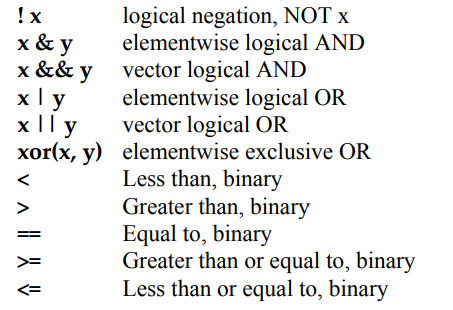
\includegraphics[width=1.5625in,height=\textheight]{images/04/01.PNG}

\begin{Shaded}
\begin{Highlighting}[]
\NormalTok{x }\OtherTok{\textless{}{-}} \DecValTok{2}
\ControlFlowTok{if}\NormalTok{(x}\SpecialCharTok{\%\%}\DecValTok{2} \SpecialCharTok{==} \DecValTok{1}\NormalTok{)\{}
  \FunctionTok{cat}\NormalTok{(}\StringTok{"Odd"}\NormalTok{)}
\NormalTok{\}}\ControlFlowTok{else}\NormalTok{\{}
  \FunctionTok{cat}\NormalTok{(}\StringTok{"Even"}\NormalTok{)}
\NormalTok{\} }

\NormalTok{x }\OtherTok{\textless{}{-}} \DecValTok{5}
\ControlFlowTok{if}\NormalTok{(x }\SpecialCharTok{\textgreater{}} \DecValTok{0} \SpecialCharTok{\&}\NormalTok{ x }\SpecialCharTok{\textless{}} \DecValTok{4}\NormalTok{)\{}
  \FunctionTok{print}\NormalTok{(}\StringTok{"Positive number less than four"}\NormalTok{)}
\NormalTok{\}}

\ControlFlowTok{if}\NormalTok{(x }\SpecialCharTok{\textgreater{}} \DecValTok{0}\NormalTok{) }\FunctionTok{print}\NormalTok{(}\StringTok{"Positive number"}\NormalTok{)}

\NormalTok{x }\OtherTok{\textless{}{-}} \SpecialCharTok{{-}}\DecValTok{5}
\ControlFlowTok{if}\NormalTok{(x }\SpecialCharTok{\textgreater{}} \DecValTok{0}\NormalTok{)\{}
  \FunctionTok{print}\NormalTok{(}\StringTok{"Non{-}negative number"}\NormalTok{)}
\NormalTok{\} }\ControlFlowTok{else} \ControlFlowTok{if}\NormalTok{(x }\SpecialCharTok{\textless{}=} \DecValTok{0} \SpecialCharTok{\&}\NormalTok{ x }\SpecialCharTok{\textgreater{}} \SpecialCharTok{{-}}\DecValTok{5}\NormalTok{)\{}
  \FunctionTok{print}\NormalTok{(}\StringTok{"Negative number greater than {-}5"}\NormalTok{)}
\NormalTok{\} }\ControlFlowTok{else}\NormalTok{ \{}
  \FunctionTok{print}\NormalTok{(}\StringTok{"Negative number less than {-}5"}\NormalTok{)}
\NormalTok{\}}

\ControlFlowTok{if}\NormalTok{(x }\SpecialCharTok{\textgreater{}} \DecValTok{0}\NormalTok{)}
  \FunctionTok{print}\NormalTok{(}\StringTok{"Non{-}negative number"}\NormalTok{)}
\ControlFlowTok{else}
  \FunctionTok{print}\NormalTok{(}\StringTok{"Negative number"}\NormalTok{)}
\end{Highlighting}
\end{Shaded}

\hypertarget{ifelse-statements}{%
\subsection{ifelse statements}\label{ifelse-statements}}

\texttt{if}는 하나의 조건만 비교하는데 사용할 수 있습니다. 그러나 변수에는 여러 값이 벡터형식으로 들어가고 벡터연산을 수행할 경우의 결과도 벡터형식으로 나오지만 \texttt{if}문은 이들을 한 번에 처리하기 어렵습니다. \texttt{ifelse}는 이러한 단점을 보완하여 여러 값을 한번에 처리할 수 있습니다.

\begin{Shaded}
\begin{Highlighting}[]
\FunctionTok{ifelse}\NormalTok{ (condition, True일 때 리턴값, False일 때 리턴값)}
\end{Highlighting}
\end{Shaded}

\texttt{ifelse}의 경우 빠르게 원하는 값을 반환할 수 있으나 조건별로 다른 추가적인 명령의 수행은 불가능하다는 단점이 있습니다.

\begin{Shaded}
\begin{Highlighting}[]

\NormalTok{x }\OtherTok{\textless{}{-}} \FunctionTok{c}\NormalTok{(}\DecValTok{1}\SpecialCharTok{:}\DecValTok{10}\NormalTok{)}
\ControlFlowTok{if}\NormalTok{(x}\SpecialCharTok{\textgreater{}}\DecValTok{10}\NormalTok{)\{}
  \FunctionTok{cat}\NormalTok{(}\StringTok{"Big"}\NormalTok{)}
\NormalTok{\}}\ControlFlowTok{else}\NormalTok{\{}
  \FunctionTok{cat}\NormalTok{(}\StringTok{"Small"}\NormalTok{)}
\NormalTok{\}}

\FunctionTok{ifelse}\NormalTok{(x}\SpecialCharTok{\textgreater{}}\DecValTok{10}\NormalTok{, }\StringTok{"Big"}\NormalTok{, }\StringTok{"Small"}\NormalTok{)}
\end{Highlighting}
\end{Shaded}

\textbf{Exercises}

다음은 median (중간값)을 구하는 공식이며 x의 길이가 (n이) 홀수일 경우와 짝수일 경우에 따라서 다른 공식이 사용된다. 다음 공식과 코드를 이용하여 mymedian 이라는 이름의 함수를 만들고 입력 값들의 중간값을 구해서 반환하는 함수를 만드시오. (\texttt{\%\%} 나머지 연산, \texttt{if}문 사용, 아래 중간값 코드 참고)

\[
median(X) =
\begin{cases}
\frac{1}{2} X[\frac{n}{2}] + \frac{1}{2} X[1+\frac{n}{2}] & \mbox{if } n \mbox{ is even} \\
X[\frac{n+1}{2}] & \mbox{if } n \mbox{ is odd}
\end{cases}
\]

\begin{Shaded}
\begin{Highlighting}[]
\NormalTok{sorted\_x }\OtherTok{\textless{}{-}} \FunctionTok{sort}\NormalTok{(x)}
\CommentTok{\# 만약 짝수이면 }
\NormalTok{retval }\OtherTok{\textless{}{-}}\NormalTok{ sort\_x[n}\SpecialCharTok{/}\DecValTok{2}\NormalTok{]}\SpecialCharTok{/}\DecValTok{2} \SpecialCharTok{+}\NormalTok{ sort\_x[}\DecValTok{1}\SpecialCharTok{+}\NormalTok{(n}\SpecialCharTok{/}\DecValTok{2}\NormalTok{)]}\SpecialCharTok{/}\DecValTok{2}
\CommentTok{\# 만약 홀수이면 }
\NormalTok{retval }\OtherTok{\textless{}{-}}\NormalTok{ sort\_x[(n}\SpecialCharTok{+}\DecValTok{1}\NormalTok{)}\SpecialCharTok{/}\DecValTok{2}\NormalTok{]}
\end{Highlighting}
\end{Shaded}

\hypertarget{for-while-repeat}{%
\subsection{for, while, repeat}\label{for-while-repeat}}

\texttt{for} 문은 반복적으로 특정 코드를 실행하고자 할 때 사용됩니다. 다음과 같은 형식으로 사용할 수 있습니다.

\begin{Shaded}
\begin{Highlighting}[]
\ControlFlowTok{for}\NormalTok{(var }\ControlFlowTok{in}\NormalTok{ seq)\{}
\NormalTok{  expression}
\NormalTok{\}}
\end{Highlighting}
\end{Shaded}

\texttt{var}는 반복을 돌 때마다 바뀌는 변수로 \texttt{\{\}} 안에서 사용되는 지역 변수 입니다. \texttt{seq}는 vector 형식의 변수로 반복을 돌 때마다 순차적으로 \texttt{var}에 저장되는 값들 입니다.

\begin{Shaded}
\begin{Highlighting}[]
\NormalTok{x }\OtherTok{\textless{}{-}} \DecValTok{1}\SpecialCharTok{:}\DecValTok{10}
\ControlFlowTok{for}\NormalTok{(i }\ControlFlowTok{in}\NormalTok{ x)\{}
  \FunctionTok{cat}\NormalTok{(i, }\StringTok{"}\SpecialCharTok{\textbackslash{}n}\StringTok{"}\NormalTok{)}
  \FunctionTok{flush.console}\NormalTok{()}
\NormalTok{\}}

\NormalTok{sum\_of\_i }\OtherTok{\textless{}{-}} \DecValTok{0}
\ControlFlowTok{for}\NormalTok{(i }\ControlFlowTok{in} \DecValTok{1}\SpecialCharTok{:}\DecValTok{10}\NormalTok{)\{}
\NormalTok{  sum\_of\_i }\OtherTok{\textless{}{-}}\NormalTok{ sum\_of\_i }\SpecialCharTok{+}\NormalTok{ i}
  \FunctionTok{cat}\NormalTok{(i, }\StringTok{" "}\NormalTok{, sum\_of\_i, }\StringTok{"}\SpecialCharTok{\textbackslash{}n}\StringTok{"}\NormalTok{);}\FunctionTok{flush.console}\NormalTok{()}
\NormalTok{\}}
\end{Highlighting}
\end{Shaded}

\texttt{while}문도 \texttt{for}문과 같이 반복적으로 특정 코드를 수행하고자 할 때 사용합니다. 사용하는 문법은 다음과 같으며 \texttt{cond}는 \texttt{True} 또는 \texttt{False} 로 반환되는 조건문을 넣고 \texttt{True} 일 경우 계속해서 반복하면서 \texttt{expressions}를 수행하며 이 반복은 \texttt{cond}가 \texttt{False}로 될 때 까지 계속됩니다.

\begin{Shaded}
\begin{Highlighting}[]
\ControlFlowTok{while}\NormalTok{(cond)\{}
\NormalTok{  expression}
\NormalTok{\}}
\end{Highlighting}
\end{Shaded}

\texttt{while}문을 사용할 경우 다음과 같이 \texttt{indicator}라 불리우는 변수를 하나 정해서 반복 할 때마다 값이 바뀌도록 해 주어야 합니다. 그렇지 않으면 무한 루프를 돌게 되는 문제가 발생합니다.

\begin{Shaded}
\begin{Highlighting}[]
\NormalTok{i }\OtherTok{\textless{}{-}} \DecValTok{10}
\NormalTok{f }\OtherTok{\textless{}{-}} \DecValTok{1}
\ControlFlowTok{while}\NormalTok{(i}\SpecialCharTok{\textgreater{}}\DecValTok{1}\NormalTok{)\{}
\NormalTok{  f }\OtherTok{\textless{}{-}}\NormalTok{ i}\SpecialCharTok{*}\NormalTok{f}
\NormalTok{  i }\OtherTok{\textless{}{-}}\NormalTok{ i}\DecValTok{{-}1}
  \FunctionTok{cat}\NormalTok{(i, f, }\StringTok{"}\SpecialCharTok{\textbackslash{}n}\StringTok{"}\NormalTok{)}
\NormalTok{\}}
\NormalTok{f}
\FunctionTok{factorial}\NormalTok{(}\DecValTok{10}\NormalTok{)}
\end{Highlighting}
\end{Shaded}

\texttt{repeat} 명령은 조건 없이 블럭 안에 있는 코드를 무조건 반복하라는 명령 입니다. 따라서 블럭 중간에 멈추기 위한 코드가 필요하고 이 명령이 \texttt{break} 입니다.

\begin{Shaded}
\begin{Highlighting}[]
\ControlFlowTok{repeat}\NormalTok{\{}
\NormalTok{  expressions}
  \ControlFlowTok{if}\NormalTok{(cond) }\ControlFlowTok{break}
\NormalTok{\}}

\NormalTok{i }\OtherTok{\textless{}{-}} \DecValTok{10}
\NormalTok{f }\OtherTok{\textless{}{-}} \DecValTok{1}
\ControlFlowTok{repeat}\NormalTok{ \{}
\NormalTok{  f }\OtherTok{\textless{}{-}}\NormalTok{ i}\SpecialCharTok{*}\NormalTok{f}
\NormalTok{  i }\OtherTok{\textless{}{-}}\NormalTok{ i}\DecValTok{{-}1}
  \FunctionTok{cat}\NormalTok{(i, f, }\StringTok{"}\SpecialCharTok{\textbackslash{}n}\StringTok{"}\NormalTok{)}
  \ControlFlowTok{if}\NormalTok{(i}\SpecialCharTok{\textless{}}\DecValTok{1}\NormalTok{) }\ControlFlowTok{break}
\NormalTok{\}}
\NormalTok{f}
\FunctionTok{factorial}\NormalTok{(}\DecValTok{10}\NormalTok{)}
\end{Highlighting}
\end{Shaded}

\hypertarget{avoiding-loops}{%
\subsection{Avoiding Loops}\label{avoiding-loops}}

R에서는 가능하면 loop문을 사용하지 않는 것이 좋습니다. 이는 다른 언어들 보다 반복문이 느리게 수행된다는 이유 때문이기도 합니다. 그러나 R에서는 반복문을 수행하는 것 보다 훨씬 더 빠르게 반복문을 수행 한 것과 같은 결과를 얻을 수 있는 다양한 방법들이 제공되고 있습니다. 차차 그런 기법들에 대한 학습을 진행하도록 하겠습니다.

\begin{Shaded}
\begin{Highlighting}[]
\NormalTok{x }\OtherTok{\textless{}{-}} \DecValTok{1}\SpecialCharTok{:}\FloatTok{1E7}
\FunctionTok{sum}\NormalTok{(x)}
\FunctionTok{system.time}\NormalTok{(}\FunctionTok{sum}\NormalTok{(x))}

\NormalTok{st }\OtherTok{\textless{}{-}} \FunctionTok{proc.time}\NormalTok{()}
\NormalTok{total }\OtherTok{\textless{}{-}} \DecValTok{0}
\ControlFlowTok{for}\NormalTok{(i }\ControlFlowTok{in} \DecValTok{1}\SpecialCharTok{:}\FunctionTok{length}\NormalTok{(x))\{}
\NormalTok{  total }\OtherTok{\textless{}{-}}\NormalTok{ total }\SpecialCharTok{+}\NormalTok{ x[i]}
\NormalTok{\}}
\NormalTok{ed }\OtherTok{\textless{}{-}} \FunctionTok{proc.time}\NormalTok{()}
\NormalTok{ed}\SpecialCharTok{{-}}\NormalTok{st}
\end{Highlighting}
\end{Shaded}

\textbf{Exercises}

\begin{enumerate}
\def\labelenumi{\arabic{enumi}.}
\tightlist
\item
  다음 네 사람의 이름과 나이를 데이터로 갖는 \texttt{users} 변수를 (data.frame) 만드시오
\end{enumerate}

\begin{Shaded}
\begin{Highlighting}[]
\NormalTok{user\_score }\OtherTok{\textless{}{-}} \FunctionTok{c}\NormalTok{(}\DecValTok{90}\NormalTok{, }\DecValTok{95}\NormalTok{, }\DecValTok{88}\NormalTok{, }\DecValTok{70}\NormalTok{)}
\NormalTok{user\_names }\OtherTok{\textless{}{-}} \FunctionTok{c}\NormalTok{(}\StringTok{"John"}\NormalTok{,}\StringTok{"James"}\NormalTok{,}\StringTok{"Sara"}\NormalTok{, }\StringTok{"Lilly"}\NormalTok{)}
\end{Highlighting}
\end{Shaded}

\begin{enumerate}
\def\labelenumi{\arabic{enumi}.}
\setcounter{enumi}{1}
\tightlist
\item
  각 사람의 점수가 80보다 작으면 \texttt{이름\ 점수:\ Fail} 크면 \texttt{이름\ 점수:\ Pass}를 출력을 하는 코드를 작성하시오. 예를 들어 John의 점수는 80보다 크므로 \texttt{John\ 90:\ Pass} 출력 (\texttt{for}, \texttt{print} 함수 이용)
\end{enumerate}

\hypertarget{object-oriented-programming-advanced}{%
\section{Object Oriented Programming (Advanced)}\label{object-oriented-programming-advanced}}

OOP는 객체지향 프로그래밍 이라고 합니다. OOP를 이용해서 프로그래밍으로 풀고자 하는 문제를 좀 더 명확하게 개념을 수립하고 복잡한 코드를 명료하게 만들 수 있습니다. 그런데 R에서 OOP는 다른 언어보다는 좀 더 어려운 개념적인 이해가 필요합니다. \texttt{S3}, \texttt{S4}, 그리고 \texttt{Reference\ class} 가 있으며 \texttt{S3}, \texttt{S4}는 \texttt{Generic\ function}을 이용하며 다른 언어에서 사용하는 OOP 개념과는 다릅니다. \texttt{Reference\ class}는 다른 언어에서 사용하는 OOP 개념과 유사하며 \texttt{R6} 패키지를 이용해서 사용할 수 있습니다.

\begin{center}\rule{0.5\linewidth}{0.5pt}\end{center}

이 저작물은 크리에이티브 커먼즈 저작자표시-비영리-변경금지 4.0 국제 라이선스에 따라 이용할 수 있습니다.

\hypertarget{data-transformation}{%
\chapter{Data transformation}\label{data-transformation}}

일반적인 데이터 분석은 데이터 전처리(변환), 가시화, 모델링(통계분석)의 반복적인 수행으로 진행될 수 있습니다. R에서는 \texttt{data.frame} 형식의 데이터 타입이 주로 사용되며 (최근 \texttt{tibble}형식) 따라서 \texttt{data.frame} 기반의 데이터를 다루기 위한 다양한 함수를 익힐 필요가 있습니다. 이번 강의에서는 \texttt{data.frame} 데이터를 읽거나 쓰는 함수들과 함께 데이터 전처리를 (변환) 위한 함수들을 배워보겠습니다.

앞에서 배웠던 데이터를 저장하는 object의 종류를 먼저 간략히 정리해 봅니다.

\begin{itemize}
\tightlist
\item
  \textbf{Vectors} - 같은 타입의 데이터를 (Numeric, character, factor, \ldots) 저장한 오브젝트로 인덱스는 \texttt{{[}}, \texttt{{]}} 사용.
\item
  \textbf{Lists} - 여러개의 \texttt{vector}를 원소로 가질 수 있으며 각 원소 vector들은 문자나 숫자 어떤 데이터 타입도 가능하고 길이가 달라도 됨. list의 인덱싱에서 \texttt{{[}} \texttt{{]}}는 리스트를 반환하고 \texttt{{[}{[}} \texttt{{]}{]}}는 vector를 반환함.
\item
  \textbf{Matrices} - 같은 타입의 데이터로 채워진 2차원 행렬이며 인덱스는 \texttt{{[}i,\ j{]}} 형태로 \texttt{i}는 row, \texttt{j}는 column 을 나타냄. 메트릭스의 생성은 \texttt{matrix} 명령어를 사용하며 왼쪽부터 column 값을 모두 채우고 다음 컬럼 값을 채워 나가는 것이 기본 설정임. \texttt{byrow=T} 를 통해 row를 먼저 채울수도 있음. row와 column 이름은 \texttt{rownames}와 \texttt{colnames}로 설정이 가능하며 \texttt{rbind}와 \texttt{cbind}로 두 행렬 또는 행렬과 백터를 연결할 수 있음 ( \texttt{rbind}와 \texttt{cbind}의 경우 행렬이 커지면 컴퓨터 리소스 많이 사용함)
\item
  \textbf{data.frame} - \texttt{list}와 \texttt{matrix}의 특성을 모두 갖는 오브젝트 타입으로 \texttt{list}와 같이 다른 타입의 \texttt{vector}형 변수 여러개가 컬럼에 붙어서 \texttt{matrix} 형태로 구성됨. 단, \texttt{list}와는 다르게 각 변수의 길이가 (row의 길이) 같아야 함. \texttt{\$} 기호로 각 변수들을 인덱싱(접근) 할 수 있고 matrix와 같이 \texttt{{[}i,j{]}} 형태의 인덱싱도 가능.
\end{itemize}

\hypertarget{reading-and-writing}{%
\section{Reading and writing}\label{reading-and-writing}}

파일에 있는 데이터를 R로 읽어들이거나 쓰는 일은 일반적인 데이터 분석 과정에서 필수적일 수 있습니다. 본 강의에서는 일반적으로 사용하는 텍스트 파일과 엑셀파일을 활용하는 방법을 알아보겠습니다.

\hypertarget{text-file}{%
\subsection{Text file}\label{text-file}}

편의상 데이터를 쓰는 과정을 먼저 살펴봅니다. \texttt{UsingR} 예제에 있는 데이터 중 \texttt{batting} 데이터는 2002 야구시즌에 선수들의 정보를 모아둔 데이터 입니다. \texttt{str} 함수로 데이터 전체적인 구조를 파악한 일부 데이터만을 (홈런 개수와 스트라이크 아웃) 이용해 추가적인 데이터를 생성한 후 별도로 파일에 저장해 보겠습니다.

\begin{Shaded}
\begin{Highlighting}[]
\FunctionTok{library}\NormalTok{(UsingR)}
\FunctionTok{data}\NormalTok{(batting)}
\FunctionTok{str}\NormalTok{(batting)}

\NormalTok{mydf }\OtherTok{\textless{}{-}} \FunctionTok{data.frame}\NormalTok{(}\AttributeTok{id =}\NormalTok{ batting}\SpecialCharTok{$}\NormalTok{playerID, }
           \AttributeTok{team =}\NormalTok{ batting}\SpecialCharTok{$}\NormalTok{teamID,}
           \AttributeTok{hr =}\NormalTok{ batting}\SpecialCharTok{$}\NormalTok{HR,}
           \AttributeTok{so =}\NormalTok{ batting}\SpecialCharTok{$}\NormalTok{SO,}
           \AttributeTok{soperhr =}\NormalTok{ batting}\SpecialCharTok{$}\NormalTok{SO}\SpecialCharTok{/}\NormalTok{batting}\SpecialCharTok{$}\NormalTok{HR)}

\FunctionTok{head}\NormalTok{(mydf)}
\end{Highlighting}
\end{Shaded}

재미삼아 홈런과 삼진아웃간의 관계를 한 번 알아보겠습니다.

\begin{Shaded}
\begin{Highlighting}[]
\FunctionTok{plot}\NormalTok{(mydf}\SpecialCharTok{$}\NormalTok{hr, mydf}\SpecialCharTok{$}\NormalTok{so)}
\NormalTok{mycor }\OtherTok{\textless{}{-}} \FunctionTok{cor}\NormalTok{(mydf}\SpecialCharTok{$}\NormalTok{hr, mydf}\SpecialCharTok{$}\NormalTok{so)}
\NormalTok{fit }\OtherTok{\textless{}{-}} \FunctionTok{lm}\NormalTok{(mydf}\SpecialCharTok{$}\NormalTok{so }\SpecialCharTok{\textasciitilde{}}\NormalTok{ mydf}\SpecialCharTok{$}\NormalTok{hr)}
\FunctionTok{plot}\NormalTok{(mydf}\SpecialCharTok{$}\NormalTok{hr, mydf}\SpecialCharTok{$}\NormalTok{so); }\FunctionTok{abline}\NormalTok{(fit); }\FunctionTok{text}\NormalTok{(}\DecValTok{50}\NormalTok{, }\DecValTok{170}\NormalTok{, }\FunctionTok{round}\NormalTok{(mycor,}\DecValTok{2}\NormalTok{))}
\end{Highlighting}
\end{Shaded}

위 데이터를 파일로 저정하기 위해서는 \texttt{write.table} 또는 \texttt{write.csv} 함수를 사용할 수 있습니다. 패키지에 따라서 다양한 함수들이 제공되고 있지만 위 두 파일은 \texttt{utils}라는 R의 기본 패키지에 들어있는 함수들로서 가장 많이 사용되는 함수들 입니다. \texttt{?write.table} 등으로 도움말을 보시고 특히 함수의 전달값 (Arguments) 들을 (\texttt{quote}, \texttt{row.names}, \texttt{col.names}, \texttt{sep}) 익혀두시기 바랍니다.

\begin{Shaded}
\begin{Highlighting}[]

\FunctionTok{write.table}\NormalTok{(mydf, }\AttributeTok{file=}\StringTok{"table\_write.txt"}\NormalTok{)}
\FunctionTok{write.table}\NormalTok{(mydf, }\AttributeTok{file=}\StringTok{"table\_write.txt"}\NormalTok{, }\AttributeTok{quote=}\NormalTok{F)}
\FunctionTok{write.table}\NormalTok{(mydf, }\AttributeTok{file=}\StringTok{"table\_write.txt"}\NormalTok{, }\AttributeTok{quote=}\NormalTok{F, }\AttributeTok{row.names=}\NormalTok{F)}
\FunctionTok{write.table}\NormalTok{(mydf, }\AttributeTok{file=}\StringTok{"table\_write.txt"}\NormalTok{, }\AttributeTok{quote=}\NormalTok{F, }\AttributeTok{row.names=}\NormalTok{F, }\AttributeTok{sep=}\StringTok{","}\NormalTok{)}
\FunctionTok{write.table}\NormalTok{(mydf, }\AttributeTok{file=}\StringTok{"table\_write.csv"}\NormalTok{, }\AttributeTok{quote=}\NormalTok{F, }\AttributeTok{row.names=}\NormalTok{F, }\AttributeTok{sep=}\StringTok{","}\NormalTok{)}
\end{Highlighting}
\end{Shaded}

대부분의 텍스트 파일은 아래와 같이 \texttt{csv} 또는 \texttt{txt} 파일로 저장하여 메모장으로 열어 확인할 수 있으며 읽어올 때 구분자 (sep 파라메터) 나 header를 (header 파라메터) 읽을지 등을 옵션으로 지정할 수 있습니다.

\begin{Shaded}
\begin{Highlighting}[]
\NormalTok{dat }\OtherTok{\textless{}{-}} \FunctionTok{read.csv}\NormalTok{(}\StringTok{"Dataset\_S1\_sub.txt"}\NormalTok{)}
\FunctionTok{head}\NormalTok{(dat)}
\end{Highlighting}
\end{Shaded}

Dataset\_S1\_sub.txt 파일을 열어보면 다음과 같이 header와 ``,''로 구분되어 있는 것을 볼 수 있습니다. \texttt{read.csv} 함수의 도움말을 보면 이 함수의 파라메터 head와 sep이 기본값으로 \texttt{T}와 \texttt{,}로 되어 있는 것을 볼 수 있습니다. \texttt{read.csv} 외에도 \texttt{read.table}, \texttt{read.delim} 등의 함수를 이용해서 택스트 파일을 읽어올 수 있습니다.

\begin{Shaded}
\begin{Highlighting}[]
\FunctionTok{str}\NormalTok{(dat)}
\end{Highlighting}
\end{Shaded}

\textbf{Exercises}

\begin{enumerate}
\def\labelenumi{\arabic{enumi}.}
\tightlist
\item
  위 \texttt{mydf}에서 가장 홈런을 많이 순서로 데이터를 정렬하시오
\item
  위 정렬된 데이터를 \texttt{mydf2} 로 저장한 후 csv 형태의 \texttt{baseball.csv} 파일로 저장하시오
\end{enumerate}

\hypertarget{excel-file}{%
\subsection{Excel file}\label{excel-file}}

텍스트 파일 외에 엑셀파일은 \texttt{readxl} 이라는 R 패키지를 활용하여 읽거나 쓸 수 있습니다. 패키지는 다음과 같은 방법으로 설치할 수 있으며 \texttt{read\_excel} 이라는 함수를 사용해서 데이터를 읽어들일 수 있습니다. 참고로 이 후 강의에서 배우게 될 \texttt{tidyverse} 패키지들 중 \texttt{readr} 패키지를 사용하여 엑셀파일 데이터를 다룰 수도 있습니다.

\begin{Shaded}
\begin{Highlighting}[]
\FunctionTok{install.packages}\NormalTok{(}\StringTok{"readxl"}\NormalTok{)}
\FunctionTok{library}\NormalTok{(readxl)}
\end{Highlighting}
\end{Shaded}

실습 파일은 형광 세포를 배양하여 형광리더기를 이용해 얻어진 실제 데이터이며 \url{plate_reader.xls} 에서 다운로드 받을 수 있습니다. \texttt{read\_excel} 함수를 이용하여 파일의 내용을 읽어오면 기본 자료형이 \texttt{tibble} 입니다. \texttt{tibble}은 최근 많이 쓰이는 R object로 \texttt{data.frame}과 유사하나 입력값의 type, name, rowname을 임으로 바꿀 수 없다는 점이 다릅니다.

\begin{Shaded}
\begin{Highlighting}[]

\NormalTok{dat }\OtherTok{\textless{}{-}} \FunctionTok{read\_excel}\NormalTok{(}\StringTok{"plate\_reader.xls"}\NormalTok{, }\AttributeTok{sheet=}\DecValTok{1}\NormalTok{, }\AttributeTok{skip =} \DecValTok{0}\NormalTok{, }\AttributeTok{col\_names=}\NormalTok{T)}
\end{Highlighting}
\end{Shaded}

엑셀파일에는 두 종류의 (\(OD600_{nm}\), Fluorescence) 데이터가 저장되어 있습니다. 첫 번째 sheet에는 다음처럼 wide형 데이터가 저장되어 있습니다.

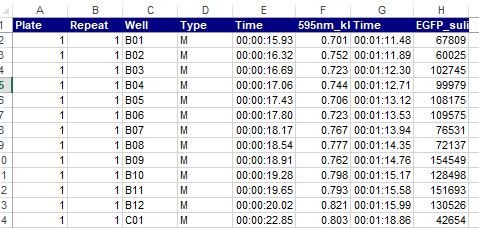
\includegraphics{images/04/excelfile01.PNG}

프로토콜 상세 내역이 나온 세 번째 시트를 읽을 경우 \texttt{sheet} 옵션을 3로 설정하면 되며 skip=3으로 하고 컬럼 이름을 별도로 사용하지 않으므로 \texttt{col\_names=T}로하여 읽을 수 있습니다.

\begin{Shaded}
\begin{Highlighting}[]

\NormalTok{dat }\OtherTok{\textless{}{-}} \FunctionTok{read\_excel}\NormalTok{(}\StringTok{"plate\_reader.xls"}\NormalTok{, }\AttributeTok{sheet=}\DecValTok{3}\NormalTok{, }\AttributeTok{skip =} \DecValTok{3}\NormalTok{, }\AttributeTok{col\_names=}\NormalTok{F)}
\end{Highlighting}
\end{Shaded}

참고로 엑셀파일로 저장하기 위해서는 csv 파일로 데이터를 writing 한 뒤 \texttt{Excel}로 해당 \texttt{csv} 파일을 열고 \texttt{xlsx} 파일로 저장할 수 있습니다.

\hypertarget{subset}{%
\section{Subset}\label{subset}}

R에서 데이터 저장은 \texttt{data.frame}이나 \texttt{matrix} 타입을 일반적으로 사용합니다. 이 데이터의 일부 열 또는 행의 데이터만을 가져와서 별도로 저장하거나 분석이 필요할 경우가 있습니다. 이 때 인덱싱을 사용해서 일부 데이터를 선택하고 사용할 수 있으며 \texttt{subset} 함수도 이러한 선별 기능을 제공합니다. \texttt{subset}은 행과 열 모두를 선별할 수 있는 함수입니다. 다음 \texttt{airquality} 데이터는 1973년 날짜별로 뉴욕의 공기질을 측정한 데이터 입니다. \texttt{NA}를 제외한 나머지 데이터만으로 새로운 데이터셋을 만들어 봅시다. \texttt{is.na}함수를 사용하면 해당 데이터가 \texttt{NA}일 경우 \texttt{TRUE}, \texttt{NA}가 아닐 경우 \texttt{FALSE} 를 반환해 줍니다.

\begin{Shaded}
\begin{Highlighting}[]
\FunctionTok{is.na}\NormalTok{(airquality}\SpecialCharTok{$}\NormalTok{Ozone)}
\NormalTok{ozone\_complete1 }\OtherTok{\textless{}{-}}\NormalTok{ airquality[}\SpecialCharTok{!}\FunctionTok{is.na}\NormalTok{(airquality}\SpecialCharTok{$}\NormalTok{Ozone),]}
\NormalTok{ozone\_complete1 }\OtherTok{\textless{}{-}} \FunctionTok{subset}\NormalTok{(airquality, }\SpecialCharTok{!}\FunctionTok{is.na}\NormalTok{(Ozone))}
\end{Highlighting}
\end{Shaded}

위 ozone\_complete1와 ozone\_complete2는 같은 결과를 보입니다. 그러나 ozone\_complete1 보다는 ozone\_complete2 코드가 훨씬 직관적이고 가독성이 높습니다. 특히 \texttt{airquality\$ozone} 로 \texttt{\$}를 사용하여 변수에 접근한 것이 아닌 \texttt{Ozone}이라는 변수 이름을 직접 사용해서 접근함으로써 코드의 간결성과 가독성을 유지할 수 있습니다. 또한 \texttt{subset}의 \texttt{select} 옵션을 이용해서 변수를 선택할 수도 있으며 \texttt{\&}(AND)와 \texttt{\textbar{}}(OR) 연산자를 사용해서 조건을 두 개 이상 설정할 수 있습니다. 아래 \texttt{select} 옵션에서 \texttt{-}는 해당 변수를 제외한다는 의미 입니다.

\begin{Shaded}
\begin{Highlighting}[]
\NormalTok{ozone\_complete3 }\OtherTok{\textless{}{-}} \FunctionTok{subset}\NormalTok{(airquality, }\SpecialCharTok{!}\FunctionTok{is.na}\NormalTok{(ozone), }\AttributeTok{select=}\FunctionTok{c}\NormalTok{(ozone, temp, month, day))}
\NormalTok{ozone\_complete4 }\OtherTok{\textless{}{-}} \FunctionTok{subset}\NormalTok{(airquality, }\SpecialCharTok{!}\FunctionTok{is.na}\NormalTok{(ozone) }\SpecialCharTok{\&} \SpecialCharTok{!}\FunctionTok{is.na}\NormalTok{(solar.r), }\AttributeTok{select=}\FunctionTok{c}\NormalTok{(}\SpecialCharTok{{-}}\NormalTok{month, }\SpecialCharTok{{-}}\NormalTok{day))}
\end{Highlighting}
\end{Shaded}

\textbf{Exercises}

airquality 데이터에서 \texttt{Temp}와 \texttt{Ozone} 변수로 이루어진 df라는 이름의 \texttt{data.frame}을 만드시오 (단 \texttt{NA}가 있는 샘플(열)은 모두 제외하시오)

\hypertarget{merging-and-split}{%
\section{Merging and Split}\label{merging-and-split}}

\texttt{merge} 함수는 두 개 이상의 데이터셋을 통합하는 기능을 수행하는 함수입니다. 특히 \texttt{rbind}나 \texttt{cbind}와는 다르게, 결합하는 두 데이터에 공통적이거나 한 쪽의 데이터를 기준으로 결합을 수행 합니다. \texttt{?merge}를 참고하면 \texttt{by}, \texttt{by.x}, \texttt{by.y}, \texttt{all}, \texttt{all.x}, \texttt{all.y} 등의 옵션으로 이러한 설정을 수행할 수 있습니다. 간단한 예제를 통해서 이해해 보겠습니다.

10명의 사람이 있고 이 사람들의 나이와 성별을 각각 나타낸 두 데이터셋이 있습니다. 그런데 df1은 나이만을 df2는 성별 정보만을 가지고 있으며 두 정보 모두 제공된 사람은 3명 (인덱스 4,5,6) 뿐입니다. 이제 merge를 이용해서 두 데이터셋을 결합해 보겠습니다.

\begin{Shaded}
\begin{Highlighting}[]
\DocumentationTok{\#\# merge}
\NormalTok{df1 }\OtherTok{\textless{}{-}} \FunctionTok{data.frame}\NormalTok{(}\AttributeTok{id=}\FunctionTok{c}\NormalTok{(}\DecValTok{1}\NormalTok{,}\DecValTok{2}\NormalTok{,}\DecValTok{3}\NormalTok{,}\DecValTok{4}\NormalTok{,}\DecValTok{5}\NormalTok{,}\DecValTok{6}\NormalTok{), }\AttributeTok{age=}\FunctionTok{c}\NormalTok{(}\DecValTok{30}\NormalTok{, }\DecValTok{41}\NormalTok{, }\DecValTok{33}\NormalTok{, }\DecValTok{56}\NormalTok{, }\DecValTok{20}\NormalTok{, }\DecValTok{17}\NormalTok{))}
\NormalTok{df2 }\OtherTok{\textless{}{-}} \FunctionTok{data.frame}\NormalTok{(}\AttributeTok{id=}\FunctionTok{c}\NormalTok{(}\DecValTok{4}\NormalTok{,}\DecValTok{5}\NormalTok{,}\DecValTok{6}\NormalTok{,}\DecValTok{7}\NormalTok{,}\DecValTok{8}\NormalTok{,}\DecValTok{9}\NormalTok{), }\AttributeTok{gender=}\FunctionTok{c}\NormalTok{(}\StringTok{"f"}\NormalTok{, }\StringTok{"f"}\NormalTok{, }\StringTok{"m"}\NormalTok{, }\StringTok{"m"}\NormalTok{, }\StringTok{"f"}\NormalTok{, }\StringTok{"m"}\NormalTok{))}

\NormalTok{df\_inner }\OtherTok{\textless{}{-}} \FunctionTok{merge}\NormalTok{(df1, df2, }\AttributeTok{by=}\StringTok{"id"}\NormalTok{, }\AttributeTok{all=}\NormalTok{F)}
\NormalTok{df\_outer }\OtherTok{\textless{}{-}} \FunctionTok{merge}\NormalTok{(df1, df2, }\AttributeTok{by=}\StringTok{"id"}\NormalTok{, }\AttributeTok{all=}\NormalTok{T)}
\NormalTok{df\_left\_outer }\OtherTok{\textless{}{-}} \FunctionTok{merge}\NormalTok{(df1, df2, }\AttributeTok{by=}\StringTok{"id"}\NormalTok{, }\AttributeTok{all.x=}\NormalTok{T)}
\NormalTok{df\_right\_outer }\OtherTok{\textless{}{-}} \FunctionTok{merge}\NormalTok{(df1, df2, }\AttributeTok{by=}\StringTok{"id"}\NormalTok{, }\AttributeTok{all.y=}\NormalTok{T)}
\end{Highlighting}
\end{Shaded}

만약 두 데이터셋의 id가 다를 경우나 각각 다른 기준으로 결합해야 하는 경우는 \texttt{by}대신 \texttt{by.x}, \texttt{by.y} 옵션을 사용할 수 있습니다.

\texttt{split} 함수는 데이터를 특정 기준으로 나누는 역할을 하며 해당 기준은 factor 형 벡터 형태로 주어질 수 있습니다. 예를 들어 \texttt{airquality} 데이터의 \texttt{month} 변수를 기준으로 데이터를 분리해 보겠습니다.

\begin{Shaded}
\begin{Highlighting}[]
\FunctionTok{str}\NormalTok{(airquality)}
\NormalTok{g }\OtherTok{\textless{}{-}} \FunctionTok{factor}\NormalTok{(airquality}\SpecialCharTok{$}\NormalTok{Month)}
\NormalTok{airq\_split }\OtherTok{\textless{}{-}} \FunctionTok{split}\NormalTok{(airquality, g)}
\FunctionTok{class}\NormalTok{(airq\_split)}
\FunctionTok{str}\NormalTok{(airq\_split)}
\end{Highlighting}
\end{Shaded}

위와 같이 \texttt{airq\_split}은 길이가 5인 (5, 6, 7, 8, 9월) \texttt{list}타입이 되었고 각 요소는 서로 다른 size의 \texttt{data.frame}형으로 구성 된 것을 확인할 수 있습니다.

\hypertarget{transformation}{%
\section{Transformation}\label{transformation}}

R에서 기존 가지고 있는 데이터의 변경은 새로운 변수의 추가, 삭제, 변형과 샘플의 추가, 삭제, 변형을 생각해 볼 수 있습니다. 이러한 기능은 앞에서 배운 \texttt{merge}, \texttt{split}이나 \texttt{rbind}, \texttt{cbind}, 그리고 인덱싱을 활용한 값 변경 등의 방법을 이용할 수 있습니다. 또한 가장 직관적으로 필요한 변수들을 기존 데이터셋에서 추출한 후 \texttt{data.frame} 명령어를 사용해서 새로운 데이터셋으로 만들어주면 될 것 입니다.

이러한 방법들 외에 \texttt{within}을 사용할 경우 특정 변수의 변형과 이를 반영한 새로운 데이터셋을 어렵지 않게 만들수 있습니다. \texttt{with} 함수의 사용 예와 함께 \texttt{within} 함수를 사용하여 데이터를 변형하는 예를 살펴봅니다. \texttt{with}나 \texttt{within} 함수는 R을 활용하는데 많이 사용되는 함수들은 아닙니다. 또한 이러한 기능들은 \texttt{dplyr} 등의 패키지에서 제공하는 경우가 많아서 필수적으로 익힐 부분은 아닙니다. 그러나 개념적인 이해를 돕기위한 좋은 도구들이며 여전히 고수준의 R 사용자들이 코드에 사용하고 있는 함수들이므로 알아두는 것이 좋습니다.

\begin{Shaded}
\begin{Highlighting}[]
\DocumentationTok{\#\# without with}
\NormalTok{ozone\_complete }\OtherTok{\textless{}{-}}\NormalTok{ airquality[}\SpecialCharTok{!}\FunctionTok{is.na}\NormalTok{(airquality}\SpecialCharTok{$}\NormalTok{Ozone),}\StringTok{"Ozone"}\NormalTok{]}
\NormalTok{temp\_complete }\OtherTok{\textless{}{-}}\NormalTok{ airquality[}\SpecialCharTok{!}\FunctionTok{is.na}\NormalTok{(airquality}\SpecialCharTok{$}\NormalTok{Temp),}\StringTok{"Temp"}\NormalTok{]}
\FunctionTok{print}\NormalTok{(}\FunctionTok{mean}\NormalTok{(ozone\_complete))}
\FunctionTok{print}\NormalTok{(}\FunctionTok{mean}\NormalTok{(temp\_complete))}

\DocumentationTok{\#\# with}
\FunctionTok{with}\NormalTok{(airquality, \{}
  \FunctionTok{print}\NormalTok{(}\FunctionTok{mean}\NormalTok{(Ozone[}\SpecialCharTok{!}\FunctionTok{is.na}\NormalTok{(Ozone)]))}
  \FunctionTok{print}\NormalTok{(}\FunctionTok{mean}\NormalTok{(Temp[}\SpecialCharTok{!}\FunctionTok{is.na}\NormalTok{(Temp)]))}
\NormalTok{\})}
\end{Highlighting}
\end{Shaded}

위 \texttt{with} 함수에서 보는바와 같이 \texttt{\$}를 이용한 변수 접근 대신 \texttt{with}함수 내에서는 (\texttt{\{}, \texttt{\}} 안에서) 해당 \texttt{data.frame}에 있는 변수 이름을 직접 접근할 수 있으며 따라서 코드의 간결함과 가독성이 향상됩니다.

\texttt{within} 함수는 \texttt{with}함수와 같이 \texttt{\{}, \texttt{\}} 안에서 변수의 이름만으로 해당 변수에 접근이 가능하나 입력된 데이터와 변경된 변수(들)을 반환한다는 점이 다릅니다. 아래 예는 \texttt{airquality} 데이터의 화씨 (Fahrenheit) 온도를 섭씨 (Celsius) 온도로 변환해서 새로운 데이터셋을 만드는 코드입니다. \texttt{data.frame}을 이용한 코드와 비교해 보시기 바랍니다. 데이터셋 내에서 참조할 변수들이 많아질 경우 \texttt{airquality\$xxx} 식의 코드를 줄이는 것 만으로도 코드의 가독성과 간결성을 유지할 수 있습니다.

\begin{Shaded}
\begin{Highlighting}[]
\NormalTok{newairquality }\OtherTok{\textless{}{-}} \FunctionTok{within}\NormalTok{(airquality, \{}
\NormalTok{  celsius }\OtherTok{=} \FunctionTok{round}\NormalTok{((}\DecValTok{5}\SpecialCharTok{*}\NormalTok{(Temp}\DecValTok{{-}32}\NormalTok{))}\SpecialCharTok{/}\DecValTok{9}\NormalTok{, }\DecValTok{2}\NormalTok{)}
\NormalTok{\})}
\FunctionTok{head}\NormalTok{(newairquality)}

\DocumentationTok{\#\# data.frame}
\NormalTok{celsius }\OtherTok{\textless{}{-}} \FunctionTok{round}\NormalTok{((}\DecValTok{5}\SpecialCharTok{*}\NormalTok{(airquality}\SpecialCharTok{$}\NormalTok{Temp}\DecValTok{{-}32}\NormalTok{))}\SpecialCharTok{/}\DecValTok{9}\NormalTok{, }\DecValTok{2}\NormalTok{)}
\NormalTok{newairquality }\OtherTok{\textless{}{-}} \FunctionTok{data.frame}\NormalTok{(airquality, celsius)}
\FunctionTok{head}\NormalTok{(newairquality)}
\end{Highlighting}
\end{Shaded}

\textbf{Exercises}

다음 df 의 hour, minute, second로 나누어진 값들을 초 단위로 변환하여 seconds라는 변수에 저장한 후 기존 df에 추가한 df2 데이터셋을 만드시오 (\texttt{within} 함수 이용)

\begin{Shaded}
\begin{Highlighting}[]
\NormalTok{df }\OtherTok{\textless{}{-}} \FunctionTok{data.frame}\NormalTok{(}\AttributeTok{hour=}\FunctionTok{c}\NormalTok{(}\DecValTok{4}\NormalTok{, }\DecValTok{7}\NormalTok{, }\DecValTok{1}\NormalTok{, }\DecValTok{5}\NormalTok{, }\DecValTok{8}\NormalTok{),}
                 \AttributeTok{minute=}\FunctionTok{c}\NormalTok{(}\DecValTok{46}\NormalTok{, }\DecValTok{56}\NormalTok{, }\DecValTok{44}\NormalTok{, }\DecValTok{37}\NormalTok{, }\DecValTok{39}\NormalTok{),}
                 \AttributeTok{second=}\FunctionTok{c}\NormalTok{(}\DecValTok{19}\NormalTok{, }\DecValTok{45}\NormalTok{, }\DecValTok{57}\NormalTok{, }\DecValTok{41}\NormalTok{, }\DecValTok{27}\NormalTok{))}
\end{Highlighting}
\end{Shaded}

\hypertarget{babies-example}{%
\section{Babies example}\label{babies-example}}

\texttt{UsingR} 패키지의 \texttt{babies} 데이터를 이용해서 산모의 흡연 여부와 신생아 몸무게의 관계를 알아보는 분석을 수행해 보겠습니다. 본 강의를 통해 배우지 않은 내용들이 있지만 코드를 따라 가면서 참고하시기 바랍니다. 우선 \texttt{UsingR} 패키지를 로딩합니다. 산모의 임신 기간이 (gestation) 999로 표기된 데이터는 명백히 에러이며 이들을 \texttt{NA}로 처리합니다.

\begin{Shaded}
\begin{Highlighting}[]
\FunctionTok{library}\NormalTok{(UsingR)}
\FunctionTok{head}\NormalTok{(babies)}
\DocumentationTok{\#\# a simple way to checkout the data}
\FunctionTok{plot}\NormalTok{(babies}\SpecialCharTok{$}\NormalTok{gestation)  }
\NormalTok{babies}\SpecialCharTok{$}\NormalTok{gestation[babies}\SpecialCharTok{$}\NormalTok{gestation}\SpecialCharTok{\textgreater{}}\DecValTok{900}\NormalTok{] }\OtherTok{\textless{}{-}} \ConstantTok{NA}
\FunctionTok{str}\NormalTok{(babies)}
\end{Highlighting}
\end{Shaded}

아래와 같이 \texttt{within} 함수를 사용해서 \texttt{babies\$} 를 반복해서 입력해주는 불편함을 줄이고 가독성을 높입니다. 똑같은 방법으로 \texttt{dwt} (아빠의 몸무게) 변수의 에러값들에 대해서도 \texttt{NA} 처리를 할 수 있습니다.

\begin{Shaded}
\begin{Highlighting}[]
\NormalTok{new\_babies }\OtherTok{\textless{}{-}} \FunctionTok{within}\NormalTok{(babies, \{}
\NormalTok{  gestation[gestation}\SpecialCharTok{==}\DecValTok{999}\NormalTok{] }\OtherTok{\textless{}{-}} \ConstantTok{NA}
\NormalTok{  dwt[dwt}\SpecialCharTok{==}\DecValTok{999}\NormalTok{] }\OtherTok{\textless{}{-}} \ConstantTok{NA}
\NormalTok{\})}
\FunctionTok{str}\NormalTok{(new\_babies)}
\end{Highlighting}
\end{Shaded}

\texttt{smoke} 변수는 흡연 여부를 나타내는 범주형 변수로 0, 1, 2, 3 값은 의미가 없습니다. 사람이 읽을 수 있는 label을 붙인 \texttt{factor} 형 변수로 변환하는 코드도 함께 작성해 보겠습니다.

\begin{Shaded}
\begin{Highlighting}[]
\FunctionTok{str}\NormalTok{(babies}\SpecialCharTok{$}\NormalTok{smoke)}
\NormalTok{new\_babies }\OtherTok{\textless{}{-}} \FunctionTok{within}\NormalTok{(babies, \{}
\NormalTok{  gestation[gestation}\SpecialCharTok{==}\DecValTok{999}\NormalTok{] }\OtherTok{\textless{}{-}} \ConstantTok{NA}
\NormalTok{  dwt[dwt}\SpecialCharTok{==}\DecValTok{999}\NormalTok{] }\OtherTok{\textless{}{-}} \ConstantTok{NA}
\NormalTok{  smoke }\OtherTok{=} \FunctionTok{factor}\NormalTok{(smoke)}
  \FunctionTok{levels}\NormalTok{(smoke) }\OtherTok{=} \FunctionTok{list}\NormalTok{(}
    \StringTok{"never"} \OtherTok{=} \DecValTok{0}\NormalTok{, }
    \StringTok{"smoke now"} \OtherTok{=} \DecValTok{1}\NormalTok{, }
    \StringTok{"until current pregnancy"} \OtherTok{=} \DecValTok{2}\NormalTok{,}
    \StringTok{"once did, not now"} \OtherTok{=} \DecValTok{3}\NormalTok{)}
\NormalTok{  \})}
\FunctionTok{str}\NormalTok{(new\_babies}\SpecialCharTok{$}\NormalTok{smoke)}
\end{Highlighting}
\end{Shaded}

이제 임신기간과 흡연 여부를 분석해 볼 수 있습니다. 흡연 그룹별로 기간에 차이가 있는지를 알아보는 분석은 \texttt{t-test}나 \texttt{ANOVA}를 사용할 수 있습니다.

\begin{Shaded}
\begin{Highlighting}[]
\NormalTok{fit }\OtherTok{\textless{}{-}} \FunctionTok{lm}\NormalTok{(gestation}\SpecialCharTok{\textasciitilde{}}\NormalTok{smoke, new\_babies)}
\FunctionTok{summary}\NormalTok{(fit) }\DocumentationTok{\#\# t{-}test 결과 }
\FunctionTok{anova}\NormalTok{(fit)}
\end{Highlighting}
\end{Shaded}

간단히 결과를 보면 \texttt{summary(fit)}은 3가지 t-test의 결과를 보여줍니다. never vs.~smoke new 의 경우 t값이 -1.657로 피우지 않은 경우에 비해서 피우는 사람의 임신 기간이 유의하게 줄어들었음을 알 수 있습니다. 그에 비해서 현재 흡연하지 않는 경우 (never vs.~until current pregnancy 또는 never vs.~once did, not now) 차이가 없는 것으로 나옵니다.

이제 smoke now 인 경우 또는 나이가 25세 미만인 경우의 샘플에 대해서 \texttt{newdf}를 만들어 봅니다 (\texttt{subset} 함수 사용, id, gestation, age, wt, smoke 변수 선택). 이 후 \texttt{ggplot}을 이용하여 몸무게와 임신기간의 산점도를 그려보면 크게 다르진 않으나 흡연하는 여성 중 몸무게가 적게 나가는 여성에게서 짧은 임신기간을 갖는 경향을 볼 수 있습니다.

\begin{Shaded}
\begin{Highlighting}[]

\NormalTok{newdf }\OtherTok{\textless{}{-}} \FunctionTok{subset}\NormalTok{(new\_babies, (smoke}\SpecialCharTok{==}\StringTok{"smoke now"} \SpecialCharTok{|}\NormalTok{ smoke }\SpecialCharTok{==} \StringTok{"never"}\NormalTok{) }\SpecialCharTok{\&}\NormalTok{ age }\SpecialCharTok{\textless{}} \DecValTok{25}\NormalTok{, }\AttributeTok{select=}\FunctionTok{c}\NormalTok{(id, gestation, age, wt, smoke))}
\CommentTok{\# ggplot(newdf, aes(x=wt, y=gestation, color=smoke)) +}
\CommentTok{\#   geom\_point(size=3, alpha=0.5) +}
\CommentTok{\#   facet\_grid(.\textasciitilde{}smoke) + }
\CommentTok{\#   theme\_bw()}
\end{Highlighting}
\end{Shaded}

\hypertarget{useful-functions-1}{%
\section{Useful functions}\label{useful-functions-1}}

지금까지 배운 여러 R 프로그래밍 기법이나 함수들과 같이 R을 활용한 데이터 분석에서 자주쓰이거나 유용하게 사용되는 함수들을 소개합니다. 먼저 원소들을 비교하여 공통적 또는 유일한 원소들만을 추출해내는 함수들 입니다.

\begin{Shaded}
\begin{Highlighting}[]
\CommentTok{\#match(), \%in\%, intersect()}

\NormalTok{x }\OtherTok{\textless{}{-}} \DecValTok{1}\SpecialCharTok{:}\DecValTok{10}
\NormalTok{y }\OtherTok{\textless{}{-}} \DecValTok{5}\SpecialCharTok{:}\DecValTok{15}
\FunctionTok{match}\NormalTok{(x, y)}
\NormalTok{x }\SpecialCharTok{\%in\%}\NormalTok{ y}
\FunctionTok{intersect}\NormalTok{(x, y)}

\CommentTok{\#unique()}
\FunctionTok{unique}\NormalTok{(}\FunctionTok{c}\NormalTok{(x, y))}
\end{Highlighting}
\end{Shaded}

다음은 스트링 관련 함수들로서 서열데이터 분석 등에서 유용하게 활용되는 함수들 입니다.

\begin{Shaded}
\begin{Highlighting}[]
\CommentTok{\#substr()}
\NormalTok{x }\OtherTok{\textless{}{-}} \StringTok{"Factors, raw vectors, and lists, are converted"}
\FunctionTok{substr}\NormalTok{(x, }\DecValTok{1}\NormalTok{, }\DecValTok{6}\NormalTok{)}

\CommentTok{\#grep()}
\FunctionTok{grep}\NormalTok{(}\StringTok{"raw"}\NormalTok{, x)}

\CommentTok{\#grepl()}
\FunctionTok{grepl}\NormalTok{(}\StringTok{"raw"}\NormalTok{, x)}
\ControlFlowTok{if}\NormalTok{(}\FunctionTok{grepl}\NormalTok{(}\StringTok{"raw"}\NormalTok{, x))\{}
  \FunctionTok{cat}\NormalTok{(}\StringTok{"I found raw!"}\NormalTok{)}
\NormalTok{\}}

\NormalTok{x }\OtherTok{\textless{}{-}} \FunctionTok{paste}\NormalTok{(LETTERS, }\DecValTok{1}\SpecialCharTok{:}\DecValTok{100}\NormalTok{, }\AttributeTok{sep=}\StringTok{""}\NormalTok{)}
\FunctionTok{grep}\NormalTok{(}\StringTok{"A"}\NormalTok{, x)}
\NormalTok{x[}\FunctionTok{grep}\NormalTok{(}\StringTok{"A"}\NormalTok{, x)]}

\FunctionTok{grepl}\NormalTok{(}\StringTok{"A"}\NormalTok{, x)}
\NormalTok{r }\OtherTok{\textless{}{-}} \FunctionTok{grepl}\NormalTok{(}\StringTok{"A"}\NormalTok{, x)}
\ControlFlowTok{if}\NormalTok{(r)\{}
  \FunctionTok{cat}\NormalTok{(}\StringTok{"Yes, I found A"}\NormalTok{)}
\NormalTok{\}}\ControlFlowTok{else}\NormalTok{\{}
  \FunctionTok{cat}\NormalTok{(}\StringTok{"No A"}\NormalTok{)}
\NormalTok{\}}

\CommentTok{\#strsplit()}
\NormalTok{x }\OtherTok{\textless{}{-}} \FunctionTok{c}\NormalTok{(}\StringTok{"Factors, raw vectors, and lists, are converted"}\NormalTok{, }\StringTok{"vectors, or for, strings with"}\NormalTok{)}
\NormalTok{y }\OtherTok{\textless{}{-}} \FunctionTok{strsplit}\NormalTok{(x, }\AttributeTok{split=}\StringTok{", "}\NormalTok{)}

\CommentTok{\#unlist()}
\FunctionTok{unlist}\NormalTok{(y)}

\NormalTok{y }\OtherTok{\textless{}{-}} \FunctionTok{strsplit}\NormalTok{(x, }\AttributeTok{split=}\StringTok{""}\NormalTok{)}
\NormalTok{ychar }\OtherTok{\textless{}{-}} \FunctionTok{unlist}\NormalTok{(y)}
\NormalTok{ycount }\OtherTok{\textless{}{-}} \FunctionTok{table}\NormalTok{(y2)}
\NormalTok{ycount\_sort }\OtherTok{\textless{}{-}} \FunctionTok{sort}\NormalTok{(ycount)}
\NormalTok{ycount\_sort }\OtherTok{\textless{}{-}} \FunctionTok{sort}\NormalTok{(ycount, }\AttributeTok{decreasing =}\NormalTok{ T)}
\NormalTok{ycount\_top }\OtherTok{\textless{}{-}}\NormalTok{ ycount\_sort[}\DecValTok{1}\SpecialCharTok{:}\DecValTok{5}\NormalTok{]}
\NormalTok{ycount\_top\_char }\OtherTok{\textless{}{-}} \FunctionTok{names}\NormalTok{(ycount\_top)}

\CommentTok{\#toupper(), tolower()}
\FunctionTok{toupper}\NormalTok{(ycount\_top\_char)}
\end{Highlighting}
\end{Shaded}

\textbf{Exercises}

built-in 데이터셋 중 \texttt{state.abb} 은 미국의 50개 주에대한 축약어임.

\begin{enumerate}
\def\labelenumi{\arabic{enumi})}
\item
  이 중 문자 A 가 들어가는 주를 뽑아 x에 저장 하시오 (\texttt{grep} 또는 \texttt{grepl} 사용)
\item
  state.abb 중 위 x에 저장된 이름들을 빼고 y에 저장 하시오 (\texttt{match()} 또는 \texttt{\%in\%}사용)
\item
  state.abb에 사용된 알파벳의 갯수를 구하고 가장 많이 쓰인 알파벳을 구하시오 (\texttt{strsplit()}, \texttt{table()} 등 사용)
\end{enumerate}

\hypertarget{apply}{%
\section{apply}\label{apply}}

\texttt{apply}는 데이터를 변형하기 위한 함수라기 보다는 데이터를 다룰 때 각 원소별, 그룹별, row, 또는 column 별로 반복적으로 수행되는 작업을 효율적으로 수행할 수 있도록 해주는 함수입니다. \texttt{apply} 계열의 함수를 적절히 사용하면 효율성이나 편리성 뿐만 아니라 코드의 간결성 등 많은 장점이 있습니다. 쉬운 이해를 위해 \texttt{colMean} 함수를 예로 들면 \texttt{colMean}은 column 또는 row 단위로 해당하는 모든 값들에 대해 평균을 계산해주는 함수이고 \texttt{apply}를 사용할 경우 다음과 같이 \texttt{apply} 함수와 \texttt{mean} 함수를 이용해서 같은 기능을 수행할 수 있습니다. 아래는 \texttt{babies} 데이터의 clearning 된 (위에서 만들었던) \texttt{new\_babies} 데이터에 이어서 수행되는 내용입니다.

\begin{Shaded}
\begin{Highlighting}[]
\FunctionTok{library}\NormalTok{(UsingR)}
\FunctionTok{head}\NormalTok{(babies)}
\NormalTok{df }\OtherTok{\textless{}{-}} \FunctionTok{subset}\NormalTok{(babies, }\AttributeTok{select=}\FunctionTok{c}\NormalTok{(gestation, wt, dwt))}
\FunctionTok{colMeans}\NormalTok{(df, }\AttributeTok{na.rm=}\NormalTok{T)}
\FunctionTok{apply}\NormalTok{(df, }\DecValTok{2}\NormalTok{, mean, }\AttributeTok{na.rm=}\NormalTok{T)}
\end{Highlighting}
\end{Shaded}

위와 같이 \texttt{colMeans}와 \texttt{apply}가 똑같은 결과를 보여주고 있습니다. 두 번째 인자인 margin의 값으로 (\texttt{?apply}참고) 여기서는 \texttt{2}가 사용되었으며 margin 값이 1인지 2인지에 따라서 다음과 같이 작동을 합니다.

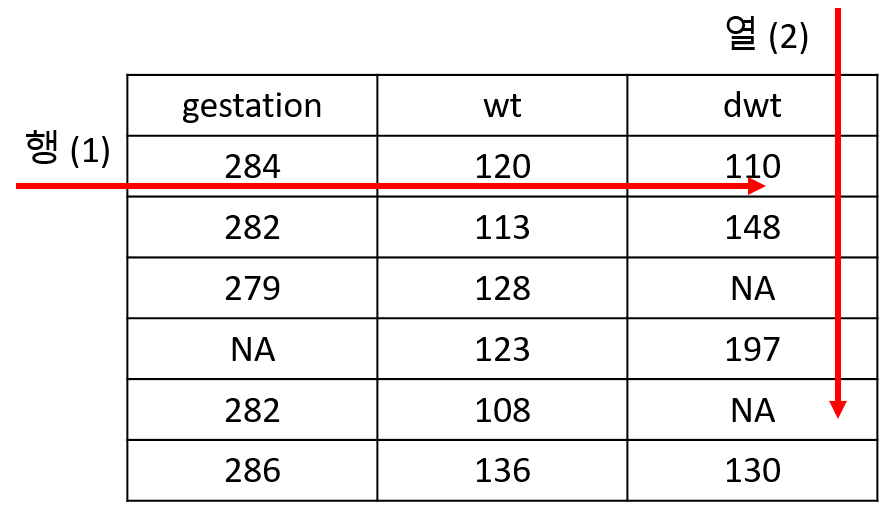
\includegraphics[width=4.16667in,height=\textheight]{images/07/01.png}

\texttt{mean}외에도 다양한 함수들이 사용될 수 있으며 아래와 같이 임의의 함수를 만들어서 사용할 수 도 있습니다. 아래 코드에서는 \texttt{function(x)...}로 바로 함수의 정의를 넣어서 사용했으나 그 아래 \texttt{mysd} 함수와 같이 미리 함수 하나를 만들고 난 후 함수 이름을 이용해서 \texttt{apply}를 적용할 수 있습니다.

\begin{Shaded}
\begin{Highlighting}[]

\FunctionTok{apply}\NormalTok{(df, }\DecValTok{2}\NormalTok{, sd, }\AttributeTok{na.rm=}\NormalTok{T)}
\FunctionTok{apply}\NormalTok{(df, }\DecValTok{2}\NormalTok{, }\ControlFlowTok{function}\NormalTok{(x)\{ }
\NormalTok{  xmean }\OtherTok{\textless{}{-}} \FunctionTok{mean}\NormalTok{(x, }\AttributeTok{na.rm=}\NormalTok{T) }
  \FunctionTok{return}\NormalTok{(xmean)}
\NormalTok{  \})}
\end{Highlighting}
\end{Shaded}

\texttt{apply} 함수는 특히 R에서 느리게 작동하는 loop (\texttt{for}, \texttt{while} 등) 문 대신 사용되어 큰 행렬에 대해서도 빠른 계산 속도를 보여줄 수 있습니다.

\begin{Shaded}
\begin{Highlighting}[]
\NormalTok{n }\OtherTok{\textless{}{-}} \DecValTok{40}
\NormalTok{m }\OtherTok{\textless{}{-}} \FunctionTok{matrix}\NormalTok{(}\FunctionTok{sample}\NormalTok{(}\DecValTok{1}\SpecialCharTok{:}\DecValTok{100}\NormalTok{, n, }\AttributeTok{replace=}\NormalTok{T), }\AttributeTok{ncol=}\DecValTok{4}\NormalTok{)}
\NormalTok{mysd }\OtherTok{\textless{}{-}} \ControlFlowTok{function}\NormalTok{(x)\{}
\NormalTok{  xmean }\OtherTok{\textless{}{-}} \FunctionTok{sum}\NormalTok{(x)}\SpecialCharTok{/}\FunctionTok{length}\NormalTok{(x)}
\NormalTok{  tmpdif }\OtherTok{\textless{}{-}}\NormalTok{ x}\SpecialCharTok{{-}}\NormalTok{xmean}
\NormalTok{  xvar }\OtherTok{\textless{}{-}} \FunctionTok{sum}\NormalTok{(tmpdif}\SpecialCharTok{\^{}}\DecValTok{2}\NormalTok{)}\SpecialCharTok{/}\NormalTok{(}\FunctionTok{length}\NormalTok{(x)}\SpecialCharTok{{-}}\DecValTok{1}\NormalTok{)}
\NormalTok{  xsd }\OtherTok{\textless{}{-}} \FunctionTok{sqrt}\NormalTok{(xvar)}
  \FunctionTok{return}\NormalTok{(xsd)}
\NormalTok{\}}

\DocumentationTok{\#\# for }
\NormalTok{results }\OtherTok{\textless{}{-}} \FunctionTok{rep}\NormalTok{(}\DecValTok{0}\NormalTok{, }\FunctionTok{nrow}\NormalTok{(m))}
\ControlFlowTok{for}\NormalTok{(i }\ControlFlowTok{in} \DecValTok{1}\SpecialCharTok{:}\FunctionTok{nrow}\NormalTok{(m))\{}
\NormalTok{  results[i] }\OtherTok{\textless{}{-}} \FunctionTok{mysd}\NormalTok{(m[i,])}
\NormalTok{\}}
\FunctionTok{print}\NormalTok{(results)}
\FunctionTok{apply}\NormalTok{(m, }\DecValTok{1}\NormalTok{, mysd)}
\FunctionTok{apply}\NormalTok{(m, }\DecValTok{1}\NormalTok{, sd)}
\end{Highlighting}
\end{Shaded}

\texttt{apply} 함수 외에도 \texttt{sapply}, \texttt{lapply}, \texttt{mapply} 등의 다양한 \texttt{apply}계열 함수가 쓰일 수 있습니다. 먼저 \texttt{lapply}는 \texttt{matrix} 형태 데이터가 아닌 \texttt{list} 데이터에 사용되어 각 \texttt{list} 원소별로 주어진 기능을 반복해서 수행하며 \texttt{sapply}는 \texttt{lapply}와 유사하나 벡터, 리스트, 데이터프레임 등에 함수를 적용할 수 있고 그 결과를 벡터 또는 행렬로 반환합니다.

\begin{Shaded}
\begin{Highlighting}[]

\NormalTok{x }\OtherTok{\textless{}{-}} \FunctionTok{list}\NormalTok{(}\AttributeTok{a=}\DecValTok{1}\SpecialCharTok{:}\DecValTok{10}\NormalTok{, }\AttributeTok{b=}\FunctionTok{exp}\NormalTok{(}\SpecialCharTok{{-}}\DecValTok{3}\SpecialCharTok{:}\DecValTok{3}\NormalTok{), }\AttributeTok{logic=}\FunctionTok{c}\NormalTok{(T,T,F,T))}
\FunctionTok{mean}\NormalTok{(x}\SpecialCharTok{$}\NormalTok{a)}
\FunctionTok{lapply}\NormalTok{(x, mean)}
\FunctionTok{sapply}\NormalTok{(x, mean)}

\NormalTok{x }\OtherTok{\textless{}{-}} \FunctionTok{data.frame}\NormalTok{(}\AttributeTok{a=}\DecValTok{1}\SpecialCharTok{:}\DecValTok{10}\NormalTok{, }\AttributeTok{b=}\FunctionTok{exp}\NormalTok{(}\SpecialCharTok{{-}}\DecValTok{4}\SpecialCharTok{:}\DecValTok{5}\NormalTok{))}
\FunctionTok{sapply}\NormalTok{(x, mean)}

\NormalTok{x }\OtherTok{\textless{}{-}} \FunctionTok{c}\NormalTok{(}\DecValTok{4}\NormalTok{, }\DecValTok{9}\NormalTok{, }\DecValTok{16}\NormalTok{)}
\FunctionTok{sapply}\NormalTok{(x, sqrt)}
\FunctionTok{sqrt}\NormalTok{(x)}

\NormalTok{y }\OtherTok{\textless{}{-}} \FunctionTok{c}\NormalTok{(}\DecValTok{1}\SpecialCharTok{:}\DecValTok{10}\NormalTok{)}
\FunctionTok{sapply}\NormalTok{(y, }\ControlFlowTok{function}\NormalTok{(x)\{}\DecValTok{2}\SpecialCharTok{*}\NormalTok{x\})}
\NormalTok{y}\SpecialCharTok{*}\DecValTok{2}
\end{Highlighting}
\end{Shaded}

마지막 예제에서처럼 \texttt{sapply}나 \texttt{lapply}도 임의의 함수를 만들어 적용시킬 수도 있습니다. 자세히 살펴 보면 y는 10개의 값을 갖는 벡터이고 이 벡터의 각 원소 (값에) 함수를 반복해서 적용하는 것 입니다. 함수에서 \texttt{x}는 각 원소의 값을 차례차례 받는 역할을 하므로 1부터 10까지 값이 함수로 들어가 2를 곱한 수가 반환됩니다. 따라서 벡터연산을 하는 \texttt{y*2}와 결과가 같으나 원하는 함수를 정의해서 자유롭게 사용할 수 있다는 장점이 있습니다. 리스트의 경우는 다음과 같이 사용합니다.

\begin{Shaded}
\begin{Highlighting}[]
\NormalTok{y }\OtherTok{\textless{}{-}} \FunctionTok{list}\NormalTok{(}\AttributeTok{a=}\DecValTok{1}\SpecialCharTok{:}\DecValTok{10}\NormalTok{, }\AttributeTok{b=}\FunctionTok{exp}\NormalTok{(}\SpecialCharTok{{-}}\DecValTok{3}\SpecialCharTok{:}\DecValTok{3}\NormalTok{), }\AttributeTok{logic=}\FunctionTok{c}\NormalTok{(T,T,F,T))}
\NormalTok{myfunc }\OtherTok{\textless{}{-}} \ControlFlowTok{function}\NormalTok{(x)\{}
  \FunctionTok{return}\NormalTok{(}\FunctionTok{mean}\NormalTok{(x, }\AttributeTok{na.rm=}\NormalTok{T))}
\NormalTok{\}}
\FunctionTok{lapply}\NormalTok{(y, myfunc)}
\FunctionTok{unlist}\NormalTok{(}\FunctionTok{lapply}\NormalTok{(y, myfunc))}
\end{Highlighting}
\end{Shaded}

즉, \texttt{myfunc}의 \texttt{x}가 list y의 각 원소들, y{[}{[}1{]}{]}, y{[}{[}2{]}{]}, y{[}{[}3{]}{]}를 각각 받아서 \texttt{mean} 연산을 수행해 줍니다. 결과로 각 \texttt{list} 원소들의 평균 값이 반환되며 \texttt{unlist} 함수는 \texttt{list} 형태의 반환 값을 \texttt{vector} 형태로 전환해 줍니다.

\textbf{Exercises}

다음은 앞에서 수행했던 \texttt{airquality} 데이터를 월별로 나눈 데이터셋임. 이 데이터셋을 이용하여 각 월별로 온도와 오존 농도의 평균값을 저장한 \texttt{data.frame} 형식의 데이터를 만들기 위하여 다음 단계별 과정에 적절한 코드를 작성하시오

\begin{Shaded}
\begin{Highlighting}[]
\DocumentationTok{\#\# dataset}
\NormalTok{g }\OtherTok{\textless{}{-}} \FunctionTok{factor}\NormalTok{(airquality}\SpecialCharTok{$}\NormalTok{month)}
\NormalTok{airq\_split }\OtherTok{\textless{}{-}} \FunctionTok{split}\NormalTok{(airquality, g)}
\end{Highlighting}
\end{Shaded}

\begin{enumerate}
\def\labelenumi{\arabic{enumi})}
\tightlist
\item
  다음 \texttt{df}의 \texttt{ozone} 평균을 구하는 \texttt{ozone\_func} 함수를 작성하시오 (단 입력은 \texttt{data.frame} 형식의 오브젝트를 받고 출력은 평균값 (정수 값 하나) 출력. \texttt{mean} 함수 사용시 데이터에 \texttt{NA}가 포함되어 있을 경우 \texttt{na.rm=T} 옵션 적용)
\end{enumerate}

\begin{Shaded}
\begin{Highlighting}[]
\DocumentationTok{\#\# May data.frame}
\NormalTok{df }\OtherTok{\textless{}{-}}\NormalTok{ airq\_split[[}\DecValTok{1}\NormalTok{]]}
\CommentTok{\#}
\CommentTok{\# write your code here for ozone\_func function}
\CommentTok{\#}

\DocumentationTok{\#\# Usage}
\FunctionTok{ozone\_func}\NormalTok{(df)}
\DocumentationTok{\#\# output}
\CommentTok{\# 23.61538}
\end{Highlighting}
\end{Shaded}

\begin{enumerate}
\def\labelenumi{\arabic{enumi})}
\setcounter{enumi}{1}
\item
  \texttt{lapply}와 \texttt{ozone\_func} 함수를 사용하여 \texttt{airq\_split} list 데이터의 월별 \texttt{ozone} 평균 값을 구하고 \texttt{ozone\_means}에 \texttt{vector} 형식으로 저장하시오
\item
  위 1), 2)와 같은 방법으로 \texttt{temp\_func} 함수를 만들고 월별 \texttt{temp}의 평균값을 \texttt{temp\_means}에 \texttt{vector} 형식으로 저장하시오.
\item
  위에서 구해진 두 변수값들을 이용하여 \texttt{air\_means} 라는 이름의 \texttt{data.frame}으로 저장하시오
\end{enumerate}

\textbf{Exercises}

\begin{enumerate}
\def\labelenumi{\arabic{enumi}.}
\tightlist
\item
  다음 코드를 이용해서 파일을 다운로드 하고 myexp에 저장하고 데이터의 구조 및 샘플들의 이름을 확인하시오
\end{enumerate}

\begin{verbatim}
myexp <- read.csv("https://github.com/greendaygh/kribbr2022/raw/main/examples/gse93819_expression_values.csv", header=T)
\end{verbatim}

\begin{enumerate}
\def\labelenumi{\arabic{enumi}.}
\setcounter{enumi}{1}
\item
  myexp의 1부터 10번째 샘플(컬럼) 데이터를 myexp1으로 11부터 20번째 샘플 데이터를 myexp2로 나누시오
\item
  myexp1의 row별 평균을 구해서 myexp1mean에 myexp2의 row별 평균을 구해서 myexp2mean에 저장하시오 (apply 이용)
\item
  myexp1mean과 myexp2mean을 합하여 myexpmean이라는 data.frame을 만드시오 (cbind이용, 주의필요)
\item
  plot을 이용하여 두 평균들의 산포도를 그리시오
\item
  myexpmean의 두 변수에 대한 차이를 구하여 mydiff 라는 변수에 저장하시오
\item
  mydiff의 값들에 대한 히스토그램 (막대그래프)을 그리시오
\end{enumerate}

\begin{center}\rule{0.5\linewidth}{0.5pt}\end{center}

이 저작물은 크리에이티브 커먼즈 저작자표시-비영리-변경금지 4.0 국제 라이선스에 따라 이용할 수 있습니다.

\hypertarget{r-basic-graphics}{%
\chapter{R basic graphics}\label{r-basic-graphics}}

\hypertarget{scatter-plot}{%
\section{scatter plot}\label{scatter-plot}}

R에서 \texttt{plot} 함수는 가장 기본이 되는 그래프 함수 입니다. 아래는 산포도를 그려주는 코드로서 myxy가 두 개의 변수(x1과 y1)를 가지고 있으므로 아래 명령들은 모두 같은 그림을 그려주게 됩니다.

\begin{Shaded}
\begin{Highlighting}[]
\NormalTok{x }\OtherTok{\textless{}{-}} \FunctionTok{c}\NormalTok{(}\DecValTok{1}\SpecialCharTok{:}\DecValTok{100}\NormalTok{)}
\NormalTok{y }\OtherTok{\textless{}{-}}\NormalTok{ x}\SpecialCharTok{*}\DecValTok{2} \SpecialCharTok{+} \FunctionTok{rnorm}\NormalTok{(}\DecValTok{100}\NormalTok{)}
\NormalTok{myxy }\OtherTok{\textless{}{-}} \FunctionTok{data.frame}\NormalTok{(x,y)}
\FunctionTok{plot}\NormalTok{(myxy)}
\FunctionTok{plot}\NormalTok{(myxy}\SpecialCharTok{$}\NormalTok{x, myxy}\SpecialCharTok{$}\NormalTok{y)}
\FunctionTok{plot}\NormalTok{(}\AttributeTok{x=}\NormalTok{myxy}\SpecialCharTok{$}\NormalTok{x, }\AttributeTok{y=}\NormalTok{myxy}\SpecialCharTok{$}\NormalTok{y)}
\FunctionTok{plot}\NormalTok{(y}\SpecialCharTok{\textasciitilde{}}\NormalTok{x, }\AttributeTok{data=}\NormalTok{myxy)}
\end{Highlighting}
\end{Shaded}

가장 마지막 명령은 \texttt{formula}를 사용한 plot으로 첫번째 파라메터 인자로 \texttt{formula} 타입이 전달되면 plot.formula 함수가 실행되며 x, y 값이 전달될 경우 \texttt{plot.default} 함수가 수행됩니다. R에서는 이렇게 전달되는 파라메터의 타입에 따라서 다른 기능을 하는 함수를 \texttt{Generic\ function} 이라고 합니다. 만약 기존 그림에 추가 데이터의 산포를 그리고 싶은 경우 \texttt{points}라는 함수를 사용합니다.

\begin{Shaded}
\begin{Highlighting}[]
\NormalTok{z }\OtherTok{\textless{}{-}} \FunctionTok{sample}\NormalTok{(}\DecValTok{1}\SpecialCharTok{:}\DecValTok{100}\NormalTok{, }\DecValTok{100}\NormalTok{, }\AttributeTok{replace =}\NormalTok{T)}
\FunctionTok{points}\NormalTok{(x, z)}
\FunctionTok{points}\NormalTok{(x, z, }\AttributeTok{col=}\StringTok{"red"}\NormalTok{)}
\end{Highlighting}
\end{Shaded}

\hypertarget{histogram}{%
\section{histogram}\label{histogram}}

\texttt{hist} 함수는 데이터들의 분포를 히스토그램으로 그려주는 함수입니다. 히스토그램은 데이터들이 갖는 값을 특정 구간으로 나누고 각 구간에 해당하는 데이터가 몇 개인지 빈도수를 계산하여 막대그래프로 보여줍니다.

\begin{Shaded}
\begin{Highlighting}[]
\NormalTok{x }\OtherTok{\textless{}{-}} \FunctionTok{rnorm}\NormalTok{(}\DecValTok{100}\NormalTok{)}
\FunctionTok{hist}\NormalTok{(x, }\AttributeTok{br=}\DecValTok{20}\NormalTok{, }\AttributeTok{xlim=}\FunctionTok{c}\NormalTok{(}\SpecialCharTok{{-}}\DecValTok{3}\NormalTok{,}\DecValTok{3}\NormalTok{), }\AttributeTok{main=}\StringTok{"Main text"}\NormalTok{, }\AttributeTok{xlab=}\StringTok{"X label"}\NormalTok{)}


\FunctionTok{hist}\NormalTok{(airquality}\SpecialCharTok{$}\NormalTok{Wind, }\AttributeTok{br=}\DecValTok{50}\NormalTok{)}
\FunctionTok{hist}\NormalTok{(airquality}\SpecialCharTok{$}\NormalTok{Wind, }\AttributeTok{br=}\DecValTok{10}\NormalTok{)}
\end{Highlighting}
\end{Shaded}

\hypertarget{boxplot}{%
\section{boxplot}\label{boxplot}}

boxplot (상자 수염 그림)은 데이터의 여러가지 대표값 (중간값 median, 첫번째 사분위수 1st quantile, 세번째 사분위수 3rd quantile, 최소 minimum, 최대값 maximum) 등을 한눈에 볼 수 있도록 만들어놓은 그래프 입니다. 수염이 나타내는 값은 최소값이나 최대값이 될 수 있고 또는 하위 1.5 IQR 에서 최소 데이터와 상위 1.5 IQR 내에 최고 데이터를 나타낼 수 있으며 이 경우 그 외에 존재하는 값들은 outlier가 됩니다.

\begin{Shaded}
\begin{Highlighting}[]
\NormalTok{x }\OtherTok{\textless{}{-}} \FunctionTok{rnorm}\NormalTok{(}\DecValTok{100}\NormalTok{)}
\FunctionTok{boxplot}\NormalTok{(x)}

\NormalTok{r }\OtherTok{\textless{}{-}} \FunctionTok{boxplot}\NormalTok{(airquality}\SpecialCharTok{$}\NormalTok{Wind)}

\NormalTok{airquality}\SpecialCharTok{$}\NormalTok{Wind[}\FunctionTok{which}\NormalTok{(airquality}\SpecialCharTok{$}\NormalTok{Wind }\SpecialCharTok{\textgreater{}}\NormalTok{ (}\FloatTok{1.5}\SpecialCharTok{*}\NormalTok{(r}\SpecialCharTok{$}\NormalTok{stats[}\DecValTok{4}\NormalTok{]}\SpecialCharTok{{-}}\NormalTok{r}\SpecialCharTok{$}\NormalTok{stats[}\DecValTok{2}\NormalTok{])}\SpecialCharTok{+}\NormalTok{r}\SpecialCharTok{$}\NormalTok{stats[}\DecValTok{4}\NormalTok{]))]}

\FunctionTok{with}\NormalTok{(airquality, \{}
\NormalTok{  Wind[}\FunctionTok{which}\NormalTok{(Wind }\SpecialCharTok{\textgreater{}}\NormalTok{ (}\FloatTok{1.5}\SpecialCharTok{*}\NormalTok{(r}\SpecialCharTok{$}\NormalTok{stats[}\DecValTok{4}\NormalTok{]}\SpecialCharTok{{-}}\NormalTok{r}\SpecialCharTok{$}\NormalTok{stats[}\DecValTok{2}\NormalTok{])}\SpecialCharTok{+}\NormalTok{r}\SpecialCharTok{$}\NormalTok{stats[}\DecValTok{4}\NormalTok{]))]}
\NormalTok{\})}

\FunctionTok{with}\NormalTok{(airquality, \{}
\NormalTok{  val }\OtherTok{\textless{}{-}}\NormalTok{ (}\FloatTok{1.5}\SpecialCharTok{*}\NormalTok{(r}\SpecialCharTok{$}\NormalTok{stats[}\DecValTok{4}\NormalTok{]}\SpecialCharTok{{-}}\NormalTok{r}\SpecialCharTok{$}\NormalTok{stats[}\DecValTok{2}\NormalTok{])}\SpecialCharTok{+}\NormalTok{r}\SpecialCharTok{$}\NormalTok{stats[}\DecValTok{4}\NormalTok{])}
\NormalTok{  Wind[}\FunctionTok{which}\NormalTok{(Wind }\SpecialCharTok{\textgreater{}}\NormalTok{ val)]}
\NormalTok{\})}

\FunctionTok{with}\NormalTok{(airquality, \{}
\NormalTok{  iqr }\OtherTok{\textless{}{-}} \FunctionTok{quantile}\NormalTok{(Wind, }\DecValTok{3}\SpecialCharTok{/}\DecValTok{4}\NormalTok{) }\SpecialCharTok{{-}} \FunctionTok{quantile}\NormalTok{(Wind, }\DecValTok{1}\SpecialCharTok{/}\DecValTok{4}\NormalTok{)}
\NormalTok{  val }\OtherTok{\textless{}{-}} \FloatTok{1.5} \SpecialCharTok{*}\NormalTok{ iqr }\SpecialCharTok{+} \FunctionTok{quantile}\NormalTok{(Wind, }\DecValTok{3}\SpecialCharTok{/}\DecValTok{4}\NormalTok{)}
\NormalTok{  Wind[}\FunctionTok{which}\NormalTok{(Wind }\SpecialCharTok{\textgreater{}}\NormalTok{ val)]}
\NormalTok{\})}
\end{Highlighting}
\end{Shaded}

data.frame 타입의 오브젝트에 대해서 boxplot을 그릴 경우 여러 변수의 데이터들의 분포를 한눈에 비교할 수 있읍니다.

\begin{Shaded}
\begin{Highlighting}[]
\NormalTok{y }\OtherTok{\textless{}{-}} \FunctionTok{rnorm}\NormalTok{(}\DecValTok{100}\NormalTok{, }\DecValTok{1}\NormalTok{, }\DecValTok{1}\NormalTok{)}
\CommentTok{\#boxplot(y)}
\NormalTok{xy }\OtherTok{\textless{}{-}} \FunctionTok{data.frame}\NormalTok{(x, y)}
\FunctionTok{boxplot}\NormalTok{(xy)}
\FunctionTok{class}\NormalTok{(xy)}

\DocumentationTok{\#\#}
\NormalTok{mean\_vals }\OtherTok{\textless{}{-}} \FunctionTok{sample}\NormalTok{(}\DecValTok{10}\NormalTok{)}
\NormalTok{mymat }\OtherTok{\textless{}{-}} \FunctionTok{sapply}\NormalTok{(mean\_vals, }\ControlFlowTok{function}\NormalTok{(x)\{}\FunctionTok{rnorm}\NormalTok{(}\DecValTok{100}\NormalTok{, x)\})}
\FunctionTok{dim}\NormalTok{(mymat)}
\FunctionTok{boxplot}\NormalTok{(mymat)}
\end{Highlighting}
\end{Shaded}

\hypertarget{barplot}{%
\section{barplot}\label{barplot}}

막대그래프는 각 값들을 막대 형태로 나란히 배치하여 서로 비교가 용이하도록 만든 그래프 입니다. \texttt{table} 함수는 같은 값을 갖는 데이터들이 몇 개나 있는지 테이블을 만들어주는 함수 입니다. rbind는 두 변수를 row를 기준으로 붙여주는 역할의 함수입니다.

\begin{Shaded}
\begin{Highlighting}[]
\NormalTok{x }\OtherTok{\textless{}{-}} \FunctionTok{sample}\NormalTok{(}\DecValTok{1}\SpecialCharTok{:}\DecValTok{12}\NormalTok{, }\DecValTok{200}\NormalTok{, }\AttributeTok{replace =}\NormalTok{ T)}
\NormalTok{tab\_x }\OtherTok{\textless{}{-}} \FunctionTok{table}\NormalTok{(x)}
\NormalTok{y }\OtherTok{\textless{}{-}} \FunctionTok{sample}\NormalTok{(}\DecValTok{1}\SpecialCharTok{:}\DecValTok{12}\NormalTok{, }\DecValTok{200}\NormalTok{, }\AttributeTok{replace =}\NormalTok{ T)}
\NormalTok{tab\_y }\OtherTok{\textless{}{-}} \FunctionTok{table}\NormalTok{(y)}
\NormalTok{tab\_xy }\OtherTok{\textless{}{-}} \FunctionTok{rbind}\NormalTok{(tab\_x, tab\_y)}
\FunctionTok{barplot}\NormalTok{(tab\_xy)}
\FunctionTok{barplot}\NormalTok{(tab\_xy, }\AttributeTok{beside =}\NormalTok{ T)}
\FunctionTok{barplot}\NormalTok{(tab\_xy, }\AttributeTok{beside =}\NormalTok{ T, }\AttributeTok{col=}\FunctionTok{c}\NormalTok{(}\StringTok{"darkblue"}\NormalTok{,}\StringTok{"red"}\NormalTok{))}
\FunctionTok{barplot}\NormalTok{(tab\_xy, }\AttributeTok{beside =}\NormalTok{ T, }\AttributeTok{col=}\FunctionTok{c}\NormalTok{(}\StringTok{"darkblue"}\NormalTok{,}\StringTok{"red"}\NormalTok{), }\AttributeTok{xlab=}\StringTok{"Month"}\NormalTok{)}
\FunctionTok{barplot}\NormalTok{(tab\_xy, }\AttributeTok{beside =}\NormalTok{ T, }\AttributeTok{col=}\FunctionTok{c}\NormalTok{(}\StringTok{"darkblue"}\NormalTok{,}\StringTok{"red"}\NormalTok{), }\AttributeTok{xlab=}\StringTok{"Month"}\NormalTok{, }\AttributeTok{horiz=}\ConstantTok{TRUE}\NormalTok{)}
\end{Highlighting}
\end{Shaded}

\textbf{Exercises}

\begin{enumerate}
\def\labelenumi{\arabic{enumi})}
\tightlist
\item
  \texttt{iris} 데이터의 꽃받침 (Sepal) 길이와 넓이를 각각 x와 y축으로 하는 산포도를 그리시오
\item
  \texttt{iris} 데이터에서 setosa 품종의 꽃받침의 (Sepal) 길이와 넓이 데이터를 빨간 점으로 나타내시오
\item
  \texttt{iris} 데이터에서 꽃받침과 (Sepal) 꽃잎의 (Petal) 길이의 분포를 그리시오 (\texttt{hist} 사용)
\item
  \texttt{iris} 데이터에서 꽃받침과 (Sepal) 꽃잎의 (Petal) 넓이의 분포를 그리시오 (\texttt{boxplot} 사용)
\item
  \texttt{iris} 데이터에서 품종별 꽃받침 (Sepal) 길이의 분포를 그리시오 (\texttt{boxplot} 사용)
\end{enumerate}

\hypertarget{draw-multiple-graphs-in-the-same-plot}{%
\section{Draw multiple graphs in the same plot}\label{draw-multiple-graphs-in-the-same-plot}}

위 예제들에서 사용한 high level function들을 low level function (\texttt{lines}, \texttt{points}, \texttt{ablines}, \texttt{axis} 등)들과 함께 사용함으로써 원하는 도표 대부분을 그려낼 수 있습니다. 최근 널리 사용되는 \texttt{ggplot2} 패키지를 이용한 그래프 사용법 강의에서는 오늘 배우는 그래픽 명령어는 거의 사용하지 않습니다. 그러나 위 함수들은 R의 기본 그래프 함수들로서 단순한 도표에서부터 복잡한 그래픽까지 구현할 수 있는 다양한 유연성을 제공하므로 기본적인 사용법을 정확히 이해하는 것이 좋습니다.

아래 도표는 평균 0, 분산 1인 분포에서 500개의 랜덤한 수를 뽑아 x에 저장하고 x의 분포를 히스토그램으로 표현한 것 입니다. 그리고 x 값들과 상관성이 있는 y값들을 (x에 2를 곱하고 평균 5, 분산 1인 랜덤하게 뽑힌 수를 노이즈로 더함) 생성하고 모든 1000개 값들의 분포를 그린 히스토그램 입니다.

\begin{Shaded}
\begin{Highlighting}[]
\NormalTok{x }\OtherTok{\textless{}{-}} \FunctionTok{rnorm}\NormalTok{(}\DecValTok{500}\NormalTok{)}
\FunctionTok{hist}\NormalTok{(x, }\DecValTok{100}\NormalTok{)}
\NormalTok{y }\OtherTok{\textless{}{-}} \DecValTok{2}\SpecialCharTok{*}\NormalTok{x }\SpecialCharTok{+} \FunctionTok{rnorm}\NormalTok{(}\DecValTok{500}\NormalTok{, }\AttributeTok{mean=}\DecValTok{5}\NormalTok{, }\AttributeTok{sd=}\DecValTok{1}\NormalTok{)}
\NormalTok{z }\OtherTok{\textless{}{-}} \FunctionTok{c}\NormalTok{(x,y)}
\FunctionTok{hist}\NormalTok{(z, }\AttributeTok{br=}\DecValTok{100}\NormalTok{)}
\end{Highlighting}
\end{Shaded}

이제 위 histogram 그래프에 \texttt{density} 함수와 \texttt{lines} 함수를 조합하여 확률밀도함수 커브를 그려 넣을 수 있습니다. 이 때 \texttt{hist} 함수에 \texttt{probability=T} 옵션을 넣어 y축의 스케일을 확률밀도함수의 y 스케일과 맞춰주어 같은 화면에 그려지도록 했습니다.

\begin{Shaded}
\begin{Highlighting}[]
\FunctionTok{hist}\NormalTok{(z, }\AttributeTok{br=}\DecValTok{100}\NormalTok{)}
\FunctionTok{hist}\NormalTok{(z, }\AttributeTok{br=}\DecValTok{100}\NormalTok{, }\AttributeTok{probability =}\NormalTok{ T)}
\NormalTok{zd }\OtherTok{\textless{}{-}} \FunctionTok{density}\NormalTok{(z)}
\FunctionTok{lines}\NormalTok{(zd)}
\end{Highlighting}
\end{Shaded}

또한 아래 그래프는 위에서 생성한 x, y 값의 산포도를 그리고 x축과 y축 범위를 xlim, ylim 파라메터로 조절하는 예제 입니다. ?pch 도움말을 참고하여 다양한 포인트 모양을 선택할 수 있으며 x 값이 0 보다 작은 경우의 index를 뽑아 해당되는 x 값들과 그 값들의 짝이 되는 y값들에 대해서만 다시 포인트 그림을 red 색상으로 그려 넣었습니다. lm 은 linear model의 약자로 회귀 곡선을 구할 때 사용하는 함수이며 이 함수를 abline과 조합하여 회귀 직선을 그릴 수 있습니다.

\begin{Shaded}
\begin{Highlighting}[]
\FunctionTok{plot}\NormalTok{(x,y, }\AttributeTok{xlim=}\FunctionTok{c}\NormalTok{(}\SpecialCharTok{{-}}\DecValTok{5}\NormalTok{, }\DecValTok{5}\NormalTok{), }\AttributeTok{ylim=}\FunctionTok{c}\NormalTok{(}\SpecialCharTok{{-}}\DecValTok{5}\NormalTok{, }\DecValTok{15}\NormalTok{), }\AttributeTok{pch=}\DecValTok{3}\NormalTok{)}
\NormalTok{idx }\OtherTok{\textless{}{-}} \FunctionTok{which}\NormalTok{(x}\SpecialCharTok{\textless{}}\DecValTok{0}\NormalTok{)}
\FunctionTok{points}\NormalTok{(x[idx], y[idx], }\AttributeTok{col=}\StringTok{"red"}\NormalTok{)}
\NormalTok{fit }\OtherTok{\textless{}{-}} \FunctionTok{lm}\NormalTok{(y}\SpecialCharTok{\textasciitilde{}}\NormalTok{x)}
\FunctionTok{abline}\NormalTok{(fit)}
\end{Highlighting}
\end{Shaded}

\textbf{Exercises}

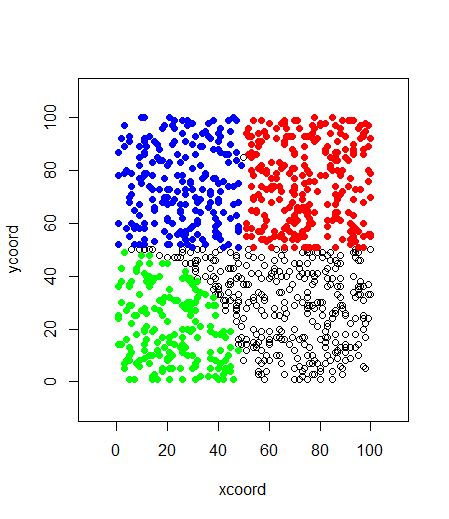
\includegraphics{images/05/01.png}

\begin{itemize}
\tightlist
\item
  1부터 100까지 수 를 랜덤하게 1000개 생성해서 x좌표를 생성하고 xcoord에 저장 하시오 (중복허용)
\item
  1부터 100까지 수 를 랜덤하게 1000개 생성해서 y좌표를 생성하고 ycoord에 저장 하시오 (중복허용)
\item
  x, y 좌표 평면에 xcoord와 ycoord 값을 이용하여 좌표를 (산포도) 그리되 x와 y의 범위가 모두 -10부터 110까지 되도록 지정 하시오 (plot 이용)
\item
  앞서 문제와 같은 plot에 x가 50보다 크고 y가 50보다 큰 곳에 있는 좌표들에 red closed circle로 표현하시오 (which, points, pch parameter 등 이용, 아래 참고)
\end{itemize}

\begin{Shaded}
\begin{Highlighting}[]
\NormalTok{idx }\OtherTok{\textless{}{-}} \FunctionTok{which}\NormalTok{(xcoord}\SpecialCharTok{\textgreater{}}\DecValTok{50} \SpecialCharTok{\&}\NormalTok{ ycoord}\SpecialCharTok{\textgreater{}}\DecValTok{50}\NormalTok{)}
\FunctionTok{points}\NormalTok{(}\AttributeTok{x=}\NormalTok{xcoord[idx], }\AttributeTok{y=}\NormalTok{ycoord[idx], }\AttributeTok{col=}\StringTok{"red"}\NormalTok{, }\AttributeTok{pch=}\DecValTok{19}\NormalTok{)}
\end{Highlighting}
\end{Shaded}

\begin{itemize}
\tightlist
\item
  앞서 문제와 같은 plot에 x가 50보다 작고 y가 50보다 큰 곳에 있는 좌표들에 blue closed circle로 표현하시오 (which, points, pch parameter 등 이용)
\item
  앞서 문제와 같은 plot에 원점으로부터 거리가 50 이하인 좌표들을 green closed circle로 표현 하시오
\end{itemize}

\hypertarget{usuful-functions-ii}{%
\section{Usuful functions II}\label{usuful-functions-ii}}

\begin{Shaded}
\begin{Highlighting}[]
\CommentTok{\#match(), \%in\%, intersect()}

\NormalTok{x }\OtherTok{\textless{}{-}} \DecValTok{1}\SpecialCharTok{:}\DecValTok{10}
\NormalTok{y }\OtherTok{\textless{}{-}} \DecValTok{5}\SpecialCharTok{:}\DecValTok{15}
\FunctionTok{match}\NormalTok{(x, y)}
\NormalTok{x }\SpecialCharTok{\%in\%}\NormalTok{ y}
\FunctionTok{intersect}\NormalTok{(x, y)}

\CommentTok{\#unique()}
\FunctionTok{unique}\NormalTok{(}\FunctionTok{c}\NormalTok{(x, y))}

\CommentTok{\#substr()}
\NormalTok{x }\OtherTok{\textless{}{-}} \StringTok{"Factors, raw vectors, and lists, are converted"}
\FunctionTok{substr}\NormalTok{(x, }\DecValTok{1}\NormalTok{, }\DecValTok{6}\NormalTok{)}

\CommentTok{\#grep()}
\FunctionTok{grep}\NormalTok{(}\StringTok{"raw"}\NormalTok{, x)}

\CommentTok{\#grepl()}
\FunctionTok{grepl}\NormalTok{(}\StringTok{"raw"}\NormalTok{, x)}
\ControlFlowTok{if}\NormalTok{(}\FunctionTok{grepl}\NormalTok{(}\StringTok{"raw"}\NormalTok{, x))\{}
  \FunctionTok{cat}\NormalTok{(}\StringTok{"I found raw!"}\NormalTok{)}
\NormalTok{\}}

\NormalTok{x }\OtherTok{\textless{}{-}} \FunctionTok{paste}\NormalTok{(LETTERS, }\DecValTok{1}\SpecialCharTok{:}\DecValTok{100}\NormalTok{, }\AttributeTok{sep=}\StringTok{""}\NormalTok{)}
\FunctionTok{grep}\NormalTok{(}\StringTok{"A"}\NormalTok{, x)}
\NormalTok{x[}\FunctionTok{grep}\NormalTok{(}\StringTok{"A"}\NormalTok{, x)]}

\FunctionTok{grepl}\NormalTok{(}\StringTok{"A"}\NormalTok{, x)}
\NormalTok{r }\OtherTok{\textless{}{-}} \FunctionTok{grepl}\NormalTok{(}\StringTok{"A"}\NormalTok{, x)}
\ControlFlowTok{if}\NormalTok{(r)\{}
  \FunctionTok{cat}\NormalTok{(}\StringTok{"Yes, I found A"}\NormalTok{)}
\NormalTok{\}}\ControlFlowTok{else}\NormalTok{\{}
  \FunctionTok{cat}\NormalTok{(}\StringTok{"No A"}\NormalTok{)}
\NormalTok{\}}

\CommentTok{\#strsplit()}
\NormalTok{x }\OtherTok{\textless{}{-}} \FunctionTok{c}\NormalTok{(}\StringTok{"Factors, raw vectors, and lists, are converted"}\NormalTok{, }\StringTok{"vectors, or for, strings with"}\NormalTok{)}
\NormalTok{y }\OtherTok{\textless{}{-}} \FunctionTok{strsplit}\NormalTok{(x, }\AttributeTok{split=}\StringTok{", "}\NormalTok{)}

\CommentTok{\#unlist()}
\FunctionTok{unlist}\NormalTok{(y)}

\NormalTok{y }\OtherTok{\textless{}{-}} \FunctionTok{strsplit}\NormalTok{(x, }\AttributeTok{split=}\StringTok{""}\NormalTok{)}
\NormalTok{ychar }\OtherTok{\textless{}{-}} \FunctionTok{unlist}\NormalTok{(y)}
\NormalTok{ycount }\OtherTok{\textless{}{-}} \FunctionTok{table}\NormalTok{(y2)}
\NormalTok{ycount\_sort }\OtherTok{\textless{}{-}} \FunctionTok{sort}\NormalTok{(ycount)}
\NormalTok{ycount\_sort }\OtherTok{\textless{}{-}} \FunctionTok{sort}\NormalTok{(ycount, }\AttributeTok{decreasing =}\NormalTok{ T)}
\NormalTok{ycount\_top }\OtherTok{\textless{}{-}}\NormalTok{ ycount\_sort[}\DecValTok{1}\SpecialCharTok{:}\DecValTok{5}\NormalTok{]}
\NormalTok{ycount\_top\_char }\OtherTok{\textless{}{-}} \FunctionTok{names}\NormalTok{(ycount\_top)}

\CommentTok{\#toupper(), tolower()}
\FunctionTok{toupper}\NormalTok{(ycount\_top\_char)}
\end{Highlighting}
\end{Shaded}

\textbf{Exercises}

built-in 데이터셋 중 \texttt{state.abb} 은 미국의 50개 주에대한 축약어임.

\begin{enumerate}
\def\labelenumi{\arabic{enumi})}
\item
  이 중 문자 A 가 들어가는 주를 뽑아 x에 저장 하시오 (\texttt{grep} 또는 \texttt{grepl} 사용)
\item
  state.abb 중 위 x에 저장된 이름들을 빼고 y에 저장 하시오 (\texttt{match()} 또는 \texttt{\%in\%}사용)
\item
  state.abb에 사용된 알파벳의 갯수를 구하고 가장 많이 쓰인 알파벳을 구하시오 (\texttt{strsplit()}, \texttt{table()} 등 사용)
\end{enumerate}

\textbf{Exercises}

\texttt{iris} 데이터셋의 각 Species 별로 꽃잎과 꽃받침의 길이와 넓이에 대한 평균값들을 구하고 막대그래프를 그리시오

\begin{enumerate}
\def\labelenumi{\arabic{enumi}.}
\tightlist
\item
  각 species 별로 데이터를 나누시오 (list 형태)
\item
  list의 각 원소 (data.frame)의 변수들의 평균을 \texttt{lapply}를 사용하여 구하시오
\item
  \texttt{do.call}과 \texttt{rbind} 함수로 list의 원소를 통합해 data.frame을 생성하시오
\item
  \texttt{barplot}을 이용하여 막대그래프를 그리시오
\end{enumerate}

\begin{center}\rule{0.5\linewidth}{0.5pt}\end{center}

이 저작물은 크리에이티브 커먼즈 저작자표시-비영리-변경금지 4.0 국제 라이선스에 따라 이용할 수 있습니다.

\hypertarget{tidyverse}{%
\chapter{tidyverse}\label{tidyverse}}

tidyverse (\url{https://www.tidyverse.org/)는} 데이터 사이언스를 위한 R 기반의 독창적인 패키지들의 모음입니다. Rstudio의 핵심 전문가인 해들리위컴이 (Hadley Wickham) 중심이 되어 만들어 졌으며 기존의 툴보다 쉽고 효율적으로 데이터 분석을 수행할 수 있습니다.

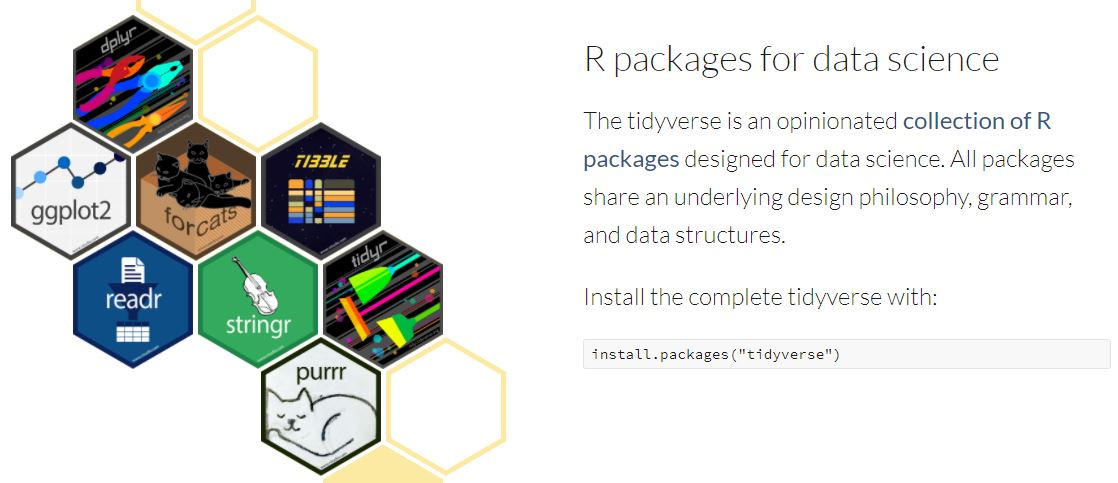
\includegraphics[width=5.72917in,height=\textheight]{images/07/tidyverse.JPG}

데이터사이언스는 넓은 범위의 개념과 방법적인 정도가 있는 것은 아닙니다. 그러나 tidyverse의 목적은 데이터 분석을 위한 핵심이되는 고효율의 툴을 제공하는 것이며 그 철학은 다음과 같은 그림으로 요약할 수 있습니다.

\begin{figure}
\centering
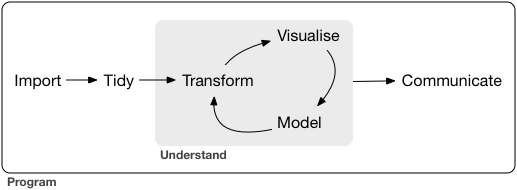
\includegraphics{images/07/data-science.png}
\caption{from \url{https://r4ds.had.co.nz/}}
\end{figure}

\hypertarget{tibble-object-type}{%
\section{tibble object type}\label{tibble-object-type}}

R은 20년 이상된 비교적 오랜 역사를 가진 언어로서 \texttt{data.frame} 형태의 데이터 타입이 가장 많이 사용되고 있습니다. 그러나 당시에는 유용했던 기능이 시간이 흐르면서 몇몇 단점들이 드러나는 문제로 기존 코드를 그대로 유지한채 package 형태로 단점을 보완한 새로운 형태의 tibble 오브젝트 형식을 만들어 냈습니다. 대부분의 R 코드는 여전히 data.frame 형태의 데이터 타입을 사용하고 있으나 tidyverse에서는 \texttt{tibble}이 사용되는 것을 참고하시기 바랍니다.

\begin{Shaded}
\begin{Highlighting}[]
\FunctionTok{library}\NormalTok{(tidyverse)}

\NormalTok{tb }\OtherTok{\textless{}{-}} \FunctionTok{tibble}\NormalTok{(}
  \AttributeTok{x =} \DecValTok{1}\SpecialCharTok{:}\DecValTok{5}\NormalTok{, }
  \AttributeTok{y =} \DecValTok{1}\NormalTok{, }
  \AttributeTok{z =}\NormalTok{ x }\SpecialCharTok{\^{}} \DecValTok{2} \SpecialCharTok{+}\NormalTok{ y}
\NormalTok{)}

\FunctionTok{as\_tibble}\NormalTok{(iris)}
\FunctionTok{head}\NormalTok{(iris)}
\end{Highlighting}
\end{Shaded}

\texttt{tibble}은 \texttt{data.frame}과 다음 몇 가지 점이 다릅니다. \texttt{data.frame}의 경우 타입을 변환할 때 강제로 값의 타입을 바꾸거나 내부 변수의 이름을 바꾸는 경우가 있었으나 \texttt{tibble}은 이를 허용하지 않습니다. 샘플들 (row) 이름을 바꿀수도 없습니다. 또한 프린팅할 때 출력물에 나오는 정보가 다르며 마지막으로 \texttt{data.frame}은 subset에 대한 타입이 바뀔 경우가 있었지만 \texttt{tibble}은 바뀌지 않습니다.

\begin{Shaded}
\begin{Highlighting}[]

\NormalTok{x }\OtherTok{\textless{}{-}} \DecValTok{1}\SpecialCharTok{:}\DecValTok{3}
\NormalTok{y }\OtherTok{\textless{}{-}} \FunctionTok{list}\NormalTok{(}\DecValTok{1}\SpecialCharTok{:}\DecValTok{5}\NormalTok{, }\DecValTok{1}\SpecialCharTok{:}\DecValTok{10}\NormalTok{, }\DecValTok{1}\SpecialCharTok{:}\DecValTok{20}\NormalTok{)}

\FunctionTok{data.frame}\NormalTok{(x, y)}
\FunctionTok{tibble}\NormalTok{(x, y)}
\end{Highlighting}
\end{Shaded}

\texttt{tibble}은 컬럼 하나가 벡터형 변수가 아닌 리스트형 변수가 될 수 있다는 것도 \texttt{data.frame}과 다른 점 입니다.

\begin{Shaded}
\begin{Highlighting}[]
\FunctionTok{names}\NormalTok{(}\FunctionTok{data.frame}\NormalTok{(}\StringTok{\textasciigrave{}}\AttributeTok{crazy name}\StringTok{\textasciigrave{}} \OtherTok{=} \DecValTok{1}\NormalTok{))}
\FunctionTok{names}\NormalTok{(}\FunctionTok{tibble}\NormalTok{(}\StringTok{\textasciigrave{}}\AttributeTok{crazy name}\StringTok{\textasciigrave{}} \OtherTok{=} \DecValTok{1}\NormalTok{))}
\end{Highlighting}
\end{Shaded}

또한 다음과 같이 사용되는 변수의 (\texttt{x}) 참조 범위가 다릅니다.

\begin{Shaded}
\begin{Highlighting}[]

\FunctionTok{data.frame}\NormalTok{(}\AttributeTok{x =} \DecValTok{1}\SpecialCharTok{:}\DecValTok{5}\NormalTok{, }\AttributeTok{y =}\NormalTok{ x }\SpecialCharTok{\^{}} \DecValTok{2}\NormalTok{)}
\FunctionTok{tibble}\NormalTok{(}\AttributeTok{x =} \DecValTok{1}\SpecialCharTok{:}\DecValTok{5}\NormalTok{, }\AttributeTok{y =}\NormalTok{ x }\SpecialCharTok{\^{}} \DecValTok{2}\NormalTok{)}
\end{Highlighting}
\end{Shaded}

\begin{Shaded}
\begin{Highlighting}[]
\NormalTok{df1 }\OtherTok{\textless{}{-}} \FunctionTok{data.frame}\NormalTok{(}\AttributeTok{x =} \DecValTok{1}\SpecialCharTok{:}\DecValTok{3}\NormalTok{, }\AttributeTok{y =} \DecValTok{3}\SpecialCharTok{:}\DecValTok{1}\NormalTok{)}
\FunctionTok{class}\NormalTok{(df1)}
\FunctionTok{class}\NormalTok{(df1[, }\DecValTok{1}\SpecialCharTok{:}\DecValTok{2}\NormalTok{])}
\FunctionTok{class}\NormalTok{(df1[, }\DecValTok{1}\NormalTok{])}

\NormalTok{df2 }\OtherTok{\textless{}{-}} \FunctionTok{tibble}\NormalTok{(}\AttributeTok{x =} \DecValTok{1}\SpecialCharTok{:}\DecValTok{3}\NormalTok{, }\AttributeTok{y =} \DecValTok{3}\SpecialCharTok{:}\DecValTok{1}\NormalTok{)}
\FunctionTok{class}\NormalTok{(df2)}
\FunctionTok{class}\NormalTok{(df2[, }\DecValTok{1}\SpecialCharTok{:}\DecValTok{2}\NormalTok{])}
\FunctionTok{class}\NormalTok{(df2[, }\DecValTok{1}\NormalTok{])}
\FunctionTok{class}\NormalTok{(df2}\SpecialCharTok{$}\NormalTok{x)}
\end{Highlighting}
\end{Shaded}

\hypertarget{tidy-data-structure}{%
\section{Tidy data structure}\label{tidy-data-structure}}

데이터의 변수와 값을 구분하는 일은 적절한 데이터 분석을 위해 필수적인 과정입니다. 특히 복잡하고 사이즈가 큰 데이터일 경우는 더욱 중요할 수 있으나 경험에 의존해서 구분을 하는 것이 대부분 입니다. Tidy data는 이러한 변수와 값의 명확한 구분과 활용을 위한 데이터 구조중 하나 입니다 (Hadley Wickham. Tidy data. \emph{The Journal of Statistical Software}, vol.~59, 2014).

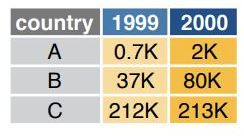
\includegraphics{images/07/notidy.JPG}

tidy data는 다음과 같은 특징이 있습니다.

\begin{itemize}
\tightlist
\item
  각 변수는 해당하는 유일한 하나의 column을 가짐
\item
  각 샘플은 해당하는 유일한 하나의 row를 가짐
\item
  각 관측값은 해당하는 유일한 하나의 cell을 가짐
\end{itemize}

\begin{figure}
\centering
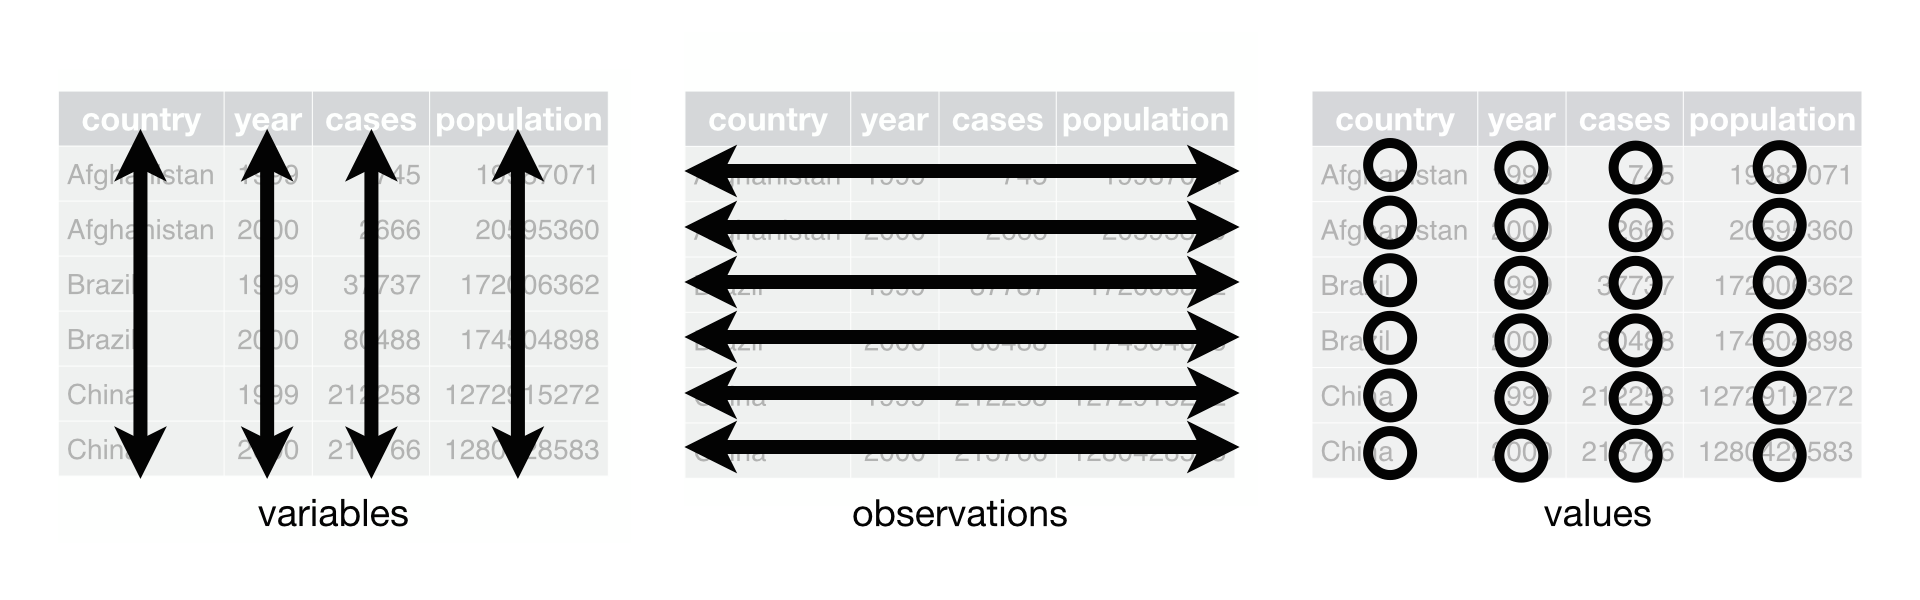
\includegraphics[width=6.25in,height=\textheight]{images/07/tidy-1.png}
\caption{from \url{https://r4ds.had.co.nz/}}
\end{figure}

Tidy 데이터는 Long형 데이터로 알려져 있기도 합니다. 참고로 Wide형 데이터의 경우 샘플 데이터가 늘어날수록 row에 쌓이고 새로운 변수는 column에 쌓이는 방식으로 데이터가 확장되는 형태 입니다. 엑셀에서 볼 수 있는 일반적인 형식으로 다음 그림과 같습니다.

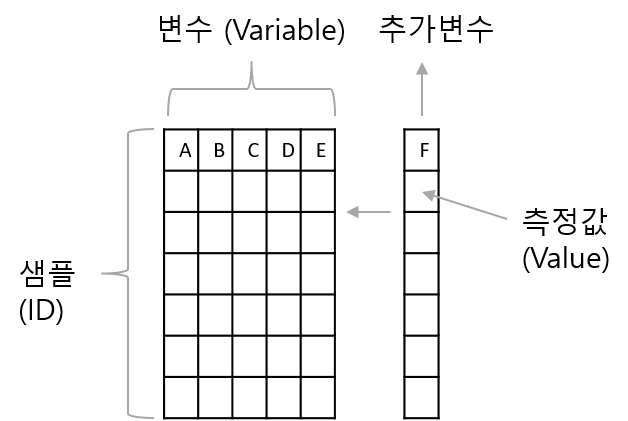
\includegraphics{images/07/05.png}

Long형 데이터의 경우 ID, variable, value 세가지 변수만 기억하면 되겠습니다. 위 wide형 데이터 경우를 보면 ID, variable, 그리고 value 이 세가지 요인이 주요 구성 요소임을 알 수 있습니다. Long형으로 변환할 경우 샘플을 참조할 수 있는 어떤 변수 (variable)도 ID가 될 수 있으며 2개 이상의 변수가 ID로 지정될 수 있습니다. 참고로 ID를 지정할 경우 해당 ID는 가능하면 중복되지 않는 값들을 갖는 변수를 사용해야 식별자로서 기능을 적절히 수행할 수 있습니다. Long형을 사용할 경우 데이터의 변수가 늘어나도 행의 수만 늘어나므로 코딩의 일관성과 변수들의 그룹을 만들어서 분석하는 등의 장점이 있습니다. 아래는 새로운 변수 F가 추가될 때 long 형 데이터에 데이터가 추가되는 경우를 나타낸 그림 입니다.

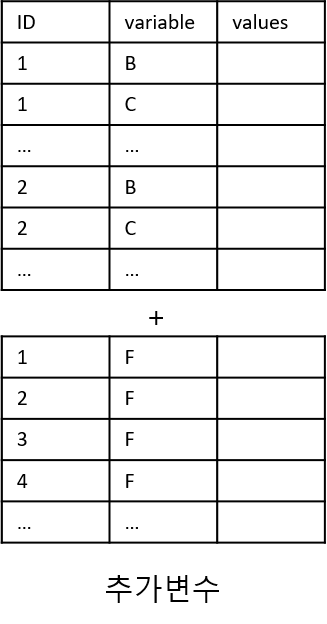
\includegraphics{images/07/06.png}

\hypertarget{pipe-operator}{%
\section{Pipe operator}\label{pipe-operator}}

tidyverse 패키지를 활용하기 위해서는 \texttt{\%\textgreater{}\%} 파이프 오퍼레이터의 이해가 필요합니다. 파이프 오퍼레이터의 작동법은 간단히 \texttt{\%\textgreater{}\%}의 왼쪽 코드의 결과를 출력으로 받아 오른쪽 코드의 입력 (첫번째 파라미터의 값)으로 받아들이는 작동을 합니다 (\textbf{단축키: Shift+Ctrl+m}). 다음 예에서 보면 \texttt{sin(pi)} 와 같은 함수의 일반적인 사용법 대신 \texttt{pi\ \%\textgreater{}\%\ sin} 처럼 사용해도 똑같은 결과를 보여줍니다. \texttt{cos(sin(pi))}와 같이 여러 합수를 중첩하여 사용할 경우와 비교해서 코드의 가독성이나 효율 측면에서 크게 향상된 방법을 제공해 줍니다.

\begin{Shaded}
\begin{Highlighting}[]
\FunctionTok{library}\NormalTok{(dplyr)}

\NormalTok{pi }\SpecialCharTok{\%\textgreater{}\%}\NormalTok{ sin}
\FunctionTok{sin}\NormalTok{(pi)}
\NormalTok{pi }\SpecialCharTok{\%\textgreater{}\%}\NormalTok{ sin }\SpecialCharTok{\%\textgreater{}\%}\NormalTok{ cos}
\FunctionTok{cos}\NormalTok{(}\FunctionTok{sin}\NormalTok{(pi))}
\end{Highlighting}
\end{Shaded}

특히 \texttt{\%\textgreater{}\%}는 이후 설명할 \texttt{dplyr}의 \texttt{group\_by}, \texttt{split}, \texttt{filter}, \texttt{summary} 등 행렬 편집/연산 함수를 빈번히 다양한 조합으로 쓰게되는 상황에서 더 큰 효과를 발휘할 수 있습니다.

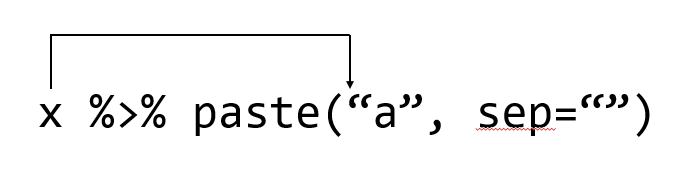
\includegraphics[width=5.20833in,height=\textheight]{images/07/02.PNG}

pipe operator의 왼쪽 구문의 결과가 오른쪽 구문의 첫 번째 파라미터의 입력 값으로 처리된다고 말씀 드렸습니다. 즉, 함수에서 사용되는 파라미터가 여러개일 경우가 있으므로 기본적으로 \texttt{\%\textgreater{}\%} 의 왼쪽 구문의 출력 값은 오른쪽 구문 (함수)의 첫 번째 인자의 입력값으로 들어가는 것 입니다. 이는 다음 예들을 통해서 명확히 알 수 있습니다. 먼저 \texttt{paste}함수는 그 파라미터로 \texttt{,}로 구분되는 여러개의 입력 값을 가질 수 있습니다. 따라서 다음 코드는 \texttt{x}가 \texttt{paste}의 첫 번째 파라미터로 들어가게 되어 \texttt{"1a",\ "2a",\ "3a",\ "4a",\ "5a"}로 a 앞에 x 값들이 붙어서 출력된 것을 알 수 있습니다.

\begin{Shaded}
\begin{Highlighting}[]
\NormalTok{x }\OtherTok{\textless{}{-}} \DecValTok{1}\SpecialCharTok{:}\DecValTok{5}
\NormalTok{x }\SpecialCharTok{\%\textgreater{}\%} \FunctionTok{paste}\NormalTok{(}\StringTok{"a"}\NormalTok{, }\AttributeTok{sep=}\StringTok{""}\NormalTok{)}
\end{Highlighting}
\end{Shaded}

특정 데이터셋의 컬럼별 평균을 구하고 각 평균의 합을 구할 경우를 생각해 봅시다. R에서는 \texttt{colMeans}라는 특별한 함수를 제공하여 컬럼별로 평균을 계산해 줍니다. 그 후 sum 함수를 사용하여 최종 원하는 값을 얻을 수 있습니다. 이러한 코드를 \texttt{\%\textgreater{}\%} 오퍼레이터를 사용한 경우의 코드와 비교해 볼 수 있습니다.

\begin{Shaded}
\begin{Highlighting}[]
\NormalTok{x }\OtherTok{\textless{}{-}} \FunctionTok{data.frame}\NormalTok{(}\AttributeTok{x=}\FunctionTok{c}\NormalTok{(}\DecValTok{1}\SpecialCharTok{:}\DecValTok{100}\NormalTok{), }\AttributeTok{y=}\FunctionTok{c}\NormalTok{(}\DecValTok{201}\SpecialCharTok{:}\DecValTok{300}\NormalTok{))}
\FunctionTok{sum}\NormalTok{(}\FunctionTok{colMeans}\NormalTok{(x))}

\NormalTok{x }\OtherTok{\textless{}{-}} \FunctionTok{data.frame}\NormalTok{(}\AttributeTok{x=}\FunctionTok{c}\NormalTok{(}\DecValTok{1}\SpecialCharTok{:}\DecValTok{100}\NormalTok{), }\AttributeTok{y=}\FunctionTok{c}\NormalTok{(}\DecValTok{201}\SpecialCharTok{:}\DecValTok{300}\NormalTok{))}
\NormalTok{x }\SpecialCharTok{\%\textgreater{}\%}\NormalTok{ colMeans }\SpecialCharTok{\%\textgreater{}\%}\NormalTok{ sum}
\end{Highlighting}
\end{Shaded}

그럼 만약 두 번째 파라미터에 입력으로 왼쪽 구문의 출력을 받아들이고 싶을 경우는 place holer \texttt{.} 을 사용하면 되겠습니다. \texttt{round} 함수는 두 개의 파라미터를 설정할 있 이으며 digits 라는 두 번째 파라미터에 값을 pipe operator로 넘겨주고 싶을 경우 아래와 같이 표현할 수 있습니다.

\begin{Shaded}
\begin{Highlighting}[]
\DecValTok{6} \SpecialCharTok{\%\textgreater{}\%} \FunctionTok{round}\NormalTok{(pi, }\AttributeTok{digits=}\NormalTok{.)}
\FunctionTok{round}\NormalTok{(pi, }\AttributeTok{digits=}\DecValTok{6}\NormalTok{)}
\end{Highlighting}
\end{Shaded}

\textbf{Exercises}

\begin{enumerate}
\def\labelenumi{\arabic{enumi})}
\tightlist
\item
  pipe operator를 사용해서 \texttt{airquality}데이터를 long형으로 전환하는 코드를 작성하시오 (단 col 파라메터에는 Ozone, Solar.R, Wind, Temp 변수를 넣음)\\
\item
  pipe operator를 사용해서 \texttt{airquality}데이터의 Month와 Day 변수(컬럼)을 Date 변수로 병합하는 코드를 작성하시오
\end{enumerate}

\hypertarget{pivoting}{%
\section{Pivoting}\label{pivoting}}

일반적으로 얻어지는 데이터의 형태는 wide형이며 이를 Long형으로 변환하기 위해서는 \texttt{tidyverse} 패키지에 속한 \texttt{tidyr} 패키지의 \texttt{pivot\_longer}와 \texttt{pivot\_wider}를 사용합니다. 또한 \texttt{reshape2} 패키지의 \texttt{melt}함수와 그 반대의 경우 \texttt{dcast} 함수를 사용할 수도 있습니다. 본 강의에서는 \texttt{tidyr} 패키지를 사용합니다. wide형 데이터를 long형으로 변환하거나 long형을 wide형으로 변환하는 작업을 pivoting 이라고 합니다.

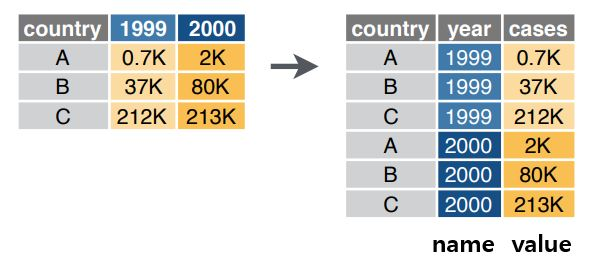
\includegraphics{images/07/wide2long.JPG}

\texttt{airquality} 데이터는 전형적인 wide형 데이터로 특정 날짜에 네 개의 변수에 해당하는 값들을 측정했습니다. 이 데이터를 long형으로 바꿀 경우 ID를 날짜로 하면 데이터들을 식별 할 수 있습니다. 그런데 날짜는 변수가 Month와 Day두 개로 나누어져 있으므로 다음과 같이 두 변수를 식별 변수로 (ID로) 사용 합니다. 확인을 위해 상위 5개의 데이터만 가지고 형 변환을 진행해 보겠습니다.

\begin{Shaded}
\begin{Highlighting}[]
\NormalTok{airquality}

\NormalTok{myair }\OtherTok{\textless{}{-}}\NormalTok{ airquality[}\DecValTok{1}\SpecialCharTok{:}\DecValTok{5}\NormalTok{,]}
\NormalTok{myair\_long }\OtherTok{\textless{}{-}} \FunctionTok{pivot\_longer}\NormalTok{(myair, }\FunctionTok{c}\NormalTok{(}\StringTok{"Ozone"}\NormalTok{, }\StringTok{"Solar.R"}\NormalTok{, }\StringTok{"Wind"}\NormalTok{, }\StringTok{"Temp"}\NormalTok{))}
\NormalTok{myair\_long }

\NormalTok{myair\_long }\OtherTok{\textless{}{-}}\NormalTok{ myair }\SpecialCharTok{\%\textgreater{}\%} 
  \FunctionTok{pivot\_longer}\NormalTok{(}\FunctionTok{c}\NormalTok{(}\StringTok{"Ozone"}\NormalTok{, }\StringTok{"Solar.R"}\NormalTok{, }\StringTok{"Wind"}\NormalTok{, }\StringTok{"Temp"}\NormalTok{))}
\NormalTok{myair\_long }

\NormalTok{myair\_long2 }\OtherTok{\textless{}{-}}\NormalTok{ myair }\SpecialCharTok{\%\textgreater{}\%} 
  \FunctionTok{pivot\_longer}\NormalTok{(}\FunctionTok{c}\NormalTok{(Ozone, Solar.R, Wind, Temp))}
\NormalTok{myair\_long2 }

\NormalTok{myair\_long3 }\OtherTok{\textless{}{-}}\NormalTok{ myair }\SpecialCharTok{\%\textgreater{}\%} 
  \FunctionTok{pivot\_longer}\NormalTok{(}\SpecialCharTok{!}\FunctionTok{c}\NormalTok{(Month, Day))}
\NormalTok{myair\_long3}
\end{Highlighting}
\end{Shaded}

생성되는 long형 데이터의 변수 이름인 name과 value는 다음 파라메터를 지정하여 바꿀 수 있습니다.

\begin{Shaded}
\begin{Highlighting}[]


\NormalTok{myair\_long }\OtherTok{\textless{}{-}}\NormalTok{ myair }\SpecialCharTok{\%\textgreater{}\%} 
  \FunctionTok{pivot\_longer}\NormalTok{(}\FunctionTok{c}\NormalTok{(Ozone, Solar.R, Wind, Temp), }
               \AttributeTok{names\_to =} \StringTok{"Type"}\NormalTok{, }
               \AttributeTok{values\_to =} \StringTok{"Observation"}\NormalTok{)}
\NormalTok{myair\_long }
\end{Highlighting}
\end{Shaded}

long형 데이터를 wide형 데이터로 변환 할 수도 있습니다.

\begin{Shaded}
\begin{Highlighting}[]
\NormalTok{myair\_long }\SpecialCharTok{\%\textgreater{}\%} 
  \FunctionTok{pivot\_wider}\NormalTok{(}
    \AttributeTok{names\_from =}\NormalTok{ Type, }
    \AttributeTok{values\_from =}\NormalTok{ Observation)}
\end{Highlighting}
\end{Shaded}

\textbf{Exercises}

\begin{enumerate}
\def\labelenumi{\arabic{enumi})}
\tightlist
\item
  다음 데이터가 long형인지 wide형인지 판단하시오\\
\item
  long형이면 wide형으로 wide형이면 long형으로 변환하시오
\end{enumerate}

\begin{Shaded}
\begin{Highlighting}[]
\NormalTok{stocks }\OtherTok{\textless{}{-}} \FunctionTok{tibble}\NormalTok{(}
  \AttributeTok{year   =} \FunctionTok{c}\NormalTok{(}\DecValTok{2015}\NormalTok{, }\DecValTok{2015}\NormalTok{, }\DecValTok{2016}\NormalTok{, }\DecValTok{2016}\NormalTok{),}
  \AttributeTok{month  =} \FunctionTok{c}\NormalTok{(   }\DecValTok{1}\NormalTok{,    }\DecValTok{2}\NormalTok{,     }\DecValTok{1}\NormalTok{,    }\DecValTok{2}\NormalTok{),}
  \AttributeTok{profit =} \FunctionTok{c}\NormalTok{(}\FloatTok{1.88}\NormalTok{, }\FloatTok{0.59}\NormalTok{, }\FloatTok{0.92}\NormalTok{, }\FloatTok{0.17}\NormalTok{)}
\NormalTok{)}
\end{Highlighting}
\end{Shaded}

\textbf{Exercises}

앞서 gse93819 데이터에서 만든 myexpmean data.frame을 long 형으로 변환하시오

\texttt{ggplot}을 이용한 그래프 작성에는 위와 같은 long형 데이터가 주로 사용됩니다. R을 이용한 데이터 가시화는 \texttt{dplyr} 패키지로 wide형 데이터를 편집하고 \texttt{pivot\_longer} 함수로 long형 데이터로 변환 후 \texttt{ggplot}을 이용하는 방식으로 수행합니다. 두 데이터 포멧에 대한 좀 더 구체적인 내용은 다음 링크를 참고하시기 바랍니다. \url{https://www.theanalysisfactor.com/wide-and-long-data/}

\hypertarget{separating-and-uniting}{%
\section{Separating and uniting}\label{separating-and-uniting}}

데이터를 분석할 때 하나의 컬럼에 두 개 이상의 변수값이 저장되어 있거나 두 개의 변수를 하나의 컬럼으로 합해야 하는 경우가 종종 있습니다. 전자의 경우 \texttt{separate()} 함수를 사용해서 두 변수(컬럼)으로 나누어 줄 수 있으며 후자의 경우 \texttt{unite()} 함수를 사용하여 두 변수를 하나의 값으로 병합할 수 있습니다. 다음은 \texttt{airquality}데이터에서 Month와 Day 변수를 하나의 컬럼으로 병합하여 Date라는 변수로 만들어 주는 경우의 예 입니다.

\begin{Shaded}
\begin{Highlighting}[]

\NormalTok{newairquality }\OtherTok{\textless{}{-}}\NormalTok{ airquality }\SpecialCharTok{\%\textgreater{}\%} 
  \FunctionTok{unite}\NormalTok{(Date, Month, Day, }\AttributeTok{sep=}\StringTok{"."}\NormalTok{)}
\NormalTok{newairquality}
\end{Highlighting}
\end{Shaded}

\texttt{separate()}함수를 사용하면 다음과 같이 해당 변수의 값을 나누어 다시 두 개의 변수(컬럼)으로 나누어 줄 수 있습니다.

\begin{Shaded}
\begin{Highlighting}[]
\NormalTok{newairquality }\SpecialCharTok{\%\textgreater{}\%} 
  \FunctionTok{separate}\NormalTok{(}\AttributeTok{col=}\NormalTok{Date, }\AttributeTok{into =} \FunctionTok{c}\NormalTok{(}\StringTok{"Month"}\NormalTok{, }\StringTok{"Day"}\NormalTok{), }\AttributeTok{sep =} \StringTok{"}\SpecialCharTok{\textbackslash{}\textbackslash{}}\StringTok{."}\NormalTok{)}
\end{Highlighting}
\end{Shaded}

\hypertarget{dplyr}{%
\section{dplyr}\label{dplyr}}

\texttt{dplyr} (\url{https://dplyr.tidyverse.org/}) 은 \texttt{ggplot2}을 개발한 해들리위컴이 (Hadley Wickham) 중심이 되어 만들어 졌으며 ggplot2와 함께 tidyverse의 (\url{https://www.tidyverse.org/}) 핵심 패키지 입니다. \texttt{dplyr}은 데이터를 다루는 크기나 분석의 속도, 편의성을 향상시켜 새롭게 만들어놓은 패키지 입니다. 기존 \texttt{apply}와 같은 행렬 연산 기능과 \texttt{subset}, \texttt{split}, \texttt{group} 와 같은 행렬 편집 기능을 더하여 만들어진 도구라고 할 수 있습니다.

\texttt{dplyr}의 전신이라 할 수 있는 \texttt{plyr} 패키지는 다음과 같이 설명이 되어 있습니다. A set of tools for a common set of problems: you need to split up a big data structure into homogeneous pieces, apply a function to each piece and then combine all the results back together. 즉 split-apply-combine 세 가지 동작을 쉽게 할 수 있도록 만들어 놓은 툴 입니다. R이 다른 언어에 비해 데이터 분석에서 주목을 받는 이유로 \texttt{split}, \texttt{apply} 등의 행렬 연산 함수가 발달한 것을 내세우는데 \texttt{dplyr}은 이들을 보다 더 편리하게 사용할 수 있도록 만들어 놓은 것 입니다.

이제 \texttt{dplyr} 패키지에서 제공하는 함수를 사용해 보겠습니다. \texttt{dplyr}을 구성하는 중요한 함수는 다음과 같습니다.

\begin{itemize}
\item
  \texttt{select()} - 변수 (columns) 선택
\item
  \texttt{filter()} - 샘플 (rows) 선택
\item
  \texttt{arrange()} - 샘플들의 정렬 순서 변경
\item
  \texttt{mutate()} - 새로운 변수 만들기
\item
  \texttt{summarise()} - 대표값 만들기
\item
  \texttt{group\_by()} - 그룹별로 계산 수행
\item
  \texttt{join()} - 두 tibble 또는 data.frame을 병합할 때 사용
\item
  위 함수들과 (특히 \texttt{filter}, \texttt{select}, \texttt{mutate}, \texttt{summarise}) 조합하여 (함수 내에서) 사용할 수 있는 helper 함수들이 같이 사용될 수 있습니다 (독립적으로도 사용 가능).

  \begin{itemize}
  \tightlist
  \item
    \texttt{across}
  \item
    \texttt{if\_any}
  \item
    \texttt{if\_all}
  \item
    \texttt{everything}
  \item
    \texttt{starts\_with}
  \item
    \texttt{end\_with}
  \item
    \texttt{contains}
  \end{itemize}
\end{itemize}

이 함수들은 \texttt{\%\textgreater{}\%}와 함께 쓰이면서 강력한 성능을 발휘합니다. \texttt{summarise} 함수는 특정 값들의 통계 값을 계산해 주는 함수이며 그 외 함수들은 행렬 편집을 위한 함수들로 보시면 되겠습니다. 간단한 예제를 수행하면서 각각의 기능을 살펴보고 왜 \texttt{dplyr}이 널리 사용되고 그 장점이 무엇인지 파악해 보도록 하겠습니다.

\texttt{iris} 데이터는 세 종류의 iris 품종에 대한 꽃잎과 꽃받침의 length와 with를 측정해 놓은 데이터 입니다. \texttt{head}와 \texttt{str} 명령어를 \texttt{\%\textgreater{}\%}를 이용해서 데이터를 살펴 봅니다.

\begin{Shaded}
\begin{Highlighting}[]
\FunctionTok{library}\NormalTok{(tidyverse)}

\NormalTok{iris }\SpecialCharTok{\%\textgreater{}\%} \FunctionTok{head}\NormalTok{(}\DecValTok{10}\NormalTok{)}
\NormalTok{iris }\SpecialCharTok{\%\textgreater{}\%}\NormalTok{ str}
\end{Highlighting}
\end{Shaded}

\hypertarget{select}{%
\subsection{select}\label{select}}

\texttt{select()} 는 주어진 데이터셋으로부터 관심있는 변수를 (column) 선택하여 보여줍니다.

\begin{Shaded}
\begin{Highlighting}[]
\FunctionTok{head}\NormalTok{(iris)}
\NormalTok{iris }\SpecialCharTok{\%\textgreater{}\%} \FunctionTok{select}\NormalTok{(Species, }\FunctionTok{everything}\NormalTok{()) }\SpecialCharTok{\%\textgreater{}\%} \FunctionTok{head}\NormalTok{(}\DecValTok{5}\NormalTok{)}
\NormalTok{iris }\SpecialCharTok{\%\textgreater{}\%} \FunctionTok{select}\NormalTok{(Species, }\FunctionTok{everything}\NormalTok{())}
\NormalTok{iris }\SpecialCharTok{\%\textgreater{}\%} \FunctionTok{select}\NormalTok{(}\SpecialCharTok{{-}}\NormalTok{Species)}
\end{Highlighting}
\end{Shaded}

\textbf{Exercises}

babies 데이터의 변수/구조를 확인해 보고 id, age, gestation, wt, dwt, smoke 변수만을 선택한 새로운 newbabies 데이터를 만드시오

다음 helper 함수들은 \texttt{select} 함수와 같이 유용하게 쓰일 수 있습니다.

\begin{quote}
starts\_with(``abc'') - ``abc'' 로 시작하는 문자열을 갖는 변수 이름
ends\_with(``xyz'') - ``xyz''으로 끝나는 문자열을 갖는 변수 이름
contains(``ijk'') - ``ijk'' 문자열을 포함하는 변수 이름
matches(``(.)\textbackslash1'') - 정규식, 반복되는 문자
\end{quote}

\begin{Shaded}
\begin{Highlighting}[]
\NormalTok{iris }\SpecialCharTok{\%\textgreater{}\%} \FunctionTok{select}\NormalTok{(}\FunctionTok{starts\_with}\NormalTok{(}\StringTok{\textquotesingle{}S\textquotesingle{}}\NormalTok{))}
\NormalTok{iris }\SpecialCharTok{\%\textgreater{}\%} \FunctionTok{select}\NormalTok{(}\AttributeTok{obs =} \FunctionTok{starts\_with}\NormalTok{(}\StringTok{\textquotesingle{}S\textquotesingle{}}\NormalTok{))}
\end{Highlighting}
\end{Shaded}

아래는 \texttt{matches} 함수를 사용한 방법 입니다. 좀 더 복잡한 패턴을 적용하여 변수들을 선택할 수 있으며 \texttt{grep} 함수를 사용할 경우도 정규식 패턴을 적용할 수 있습니다.

\begin{Shaded}
\begin{Highlighting}[]
\NormalTok{iris2 }\OtherTok{\textless{}{-}} \FunctionTok{rename}\NormalTok{(iris, }\AttributeTok{aavar =}\NormalTok{ Petal.Length)}
\FunctionTok{select}\NormalTok{(iris2, }\FunctionTok{matches}\NormalTok{(}\StringTok{"(.)}\SpecialCharTok{\textbackslash{}\textbackslash{}}\StringTok{1"}\NormalTok{))}
\NormalTok{tmp }\OtherTok{\textless{}{-}}\NormalTok{iris[,}\DecValTok{3}\SpecialCharTok{:}\DecValTok{5}\NormalTok{]}
\FunctionTok{colnames}\NormalTok{(iris)[}\FunctionTok{grep}\NormalTok{(}\StringTok{"\^{}S"}\NormalTok{, }\FunctionTok{colnames}\NormalTok{(iris))]}
\NormalTok{iris[,}\FunctionTok{grep}\NormalTok{(}\StringTok{"\^{}S"}\NormalTok{, }\FunctionTok{colnames}\NormalTok{(iris))]}
\NormalTok{tmp}
\end{Highlighting}
\end{Shaded}

아래 \texttt{(.)\textbackslash{}\textbackslash{}1}은 하나의 문자 \texttt{.}가 (어떤 문자든) 한 번 더 \texttt{\textbackslash{}\textbackslash{}1} 사용된 변수 이름을 말하며 이는 \texttt{aavar} 의 \texttt{aa}밖에 없으므로 \texttt{aavar}가 선택됩니다. \texttt{grep}에서 \texttt{\^{}} 표시는 맨 처음을 나타내므로 \texttt{\^{}S}는 S로 시작하는 문자가 되겠습니다. 따라서 \texttt{grep("\^{}S",\ colnames(iris))}의 경우 컬럼 이름 중 S로 시작하는 이름은 True로 그렇지 않으면 False 값을 리턴합니다.

\hypertarget{filter}{%
\subsection{filter}\label{filter}}

\texttt{filter} 함수를 사용해서 원하는 조건의 데이터 (샘플)을 골라낼 수 있습니다.

\begin{Shaded}
\begin{Highlighting}[]
\FunctionTok{library}\NormalTok{(dplyr)}

\FunctionTok{head}\NormalTok{(iris)}
\NormalTok{iris }\SpecialCharTok{\%\textgreater{}\%} 
  \FunctionTok{filter}\NormalTok{(Species}\SpecialCharTok{==}\StringTok{"setosa"}\NormalTok{)}

\NormalTok{iris }\SpecialCharTok{\%\textgreater{}\%} 
  \FunctionTok{filter}\NormalTok{(Species}\SpecialCharTok{==}\StringTok{"setosa"} \SpecialCharTok{|}\NormalTok{ Species}\SpecialCharTok{==}\StringTok{"versicolor"}\NormalTok{)}

\NormalTok{iris }\SpecialCharTok{\%\textgreater{}\%} 
  \FunctionTok{filter}\NormalTok{(Species}\SpecialCharTok{==}\StringTok{"setosa"} \SpecialCharTok{\&}\NormalTok{ Species}\SpecialCharTok{==}\StringTok{"versicolor"}\NormalTok{)}

\NormalTok{iris }\SpecialCharTok{\%\textgreater{}\%} 
  \FunctionTok{filter}\NormalTok{(Species}\SpecialCharTok{==}\StringTok{"setosa"} \SpecialCharTok{|}\NormalTok{ Species}\SpecialCharTok{==}\StringTok{"versicolor"}\NormalTok{) }\SpecialCharTok{\%\textgreater{}\%} 
\NormalTok{  dim}
\end{Highlighting}
\end{Shaded}

\texttt{filter}의 \texttt{,}로 구분되는 매개변수는 \texttt{and} 로직으로 묶인 조건입니다. 지난 강좌에서 보셨듯 R에서 \texttt{and}는 \texttt{\&}, \texttt{or}는 \texttt{\textbar{}}, 그리고 not은 \texttt{!} 으로 사용하면 되며 \texttt{filter}에서 \texttt{,}로 구분된 조건은 \texttt{and}와 같다고 보시면 되겠습니다.

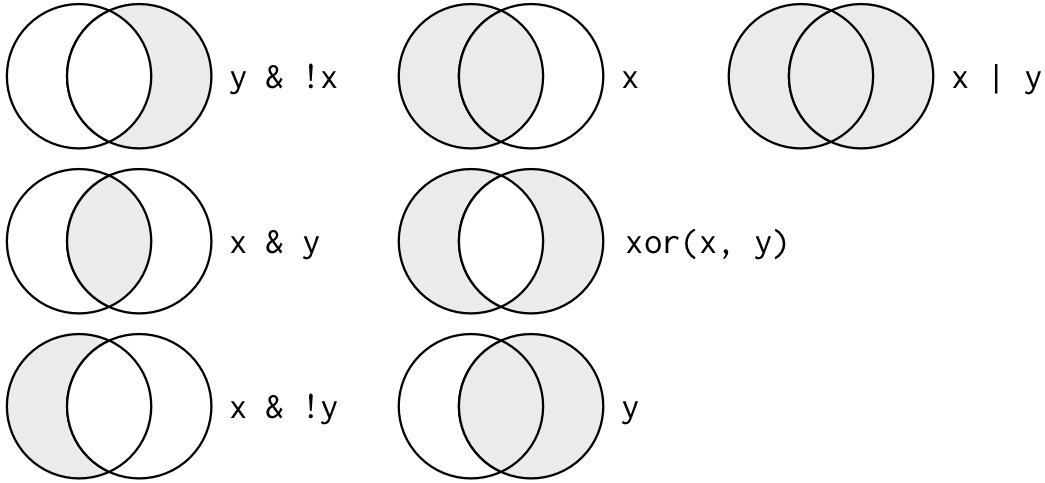
\includegraphics[width=5.20833in,height=\textheight]{images/07/03.png}

Image from (\url{https://r4ds.had.co.nz/})

\textbf{Exercises}

위 예제에서 만든 newbabies 데이터에서 999 값이 들어있는 값을 제외한 새로운 데이터를 만드시오

\hypertarget{arrange}{%
\subsection{arrange}\label{arrange}}

\texttt{arrange()}는 지정된 변수를 기준으로 값의 크기순서로 샘플들의 배열 순서 즉, row의 순서를 바꾸는 기능을 수행합니다. 기본으로 크기가 커지는 순서로 정렬이 진행되며 작아지는 순서를 원할 경우 \texttt{desc} 함수를 사용할 수 있습니다.

\begin{Shaded}
\begin{Highlighting}[]
\NormalTok{iris }\SpecialCharTok{\%\textgreater{}\%} \FunctionTok{arrange}\NormalTok{(Sepal.Length)}
\NormalTok{iris }\SpecialCharTok{\%\textgreater{}\%} \FunctionTok{arrange}\NormalTok{(}\FunctionTok{desc}\NormalTok{(Sepal.Length))}
\NormalTok{iris }\SpecialCharTok{\%\textgreater{}\%} \FunctionTok{arrange}\NormalTok{(Sepal.Length, Sepal.Width)}
\end{Highlighting}
\end{Shaded}

\hypertarget{mutate}{%
\subsection{mutate}\label{mutate}}

\texttt{mutate()} 함수는 새로운 변수를 추가할 수 있는 기능을 제공하며 앞에서 배웠던 \texttt{within()}과 비슷하다고 볼 수 있습니다. 아래와 같이 \texttt{mutate}함수는 sepal\_ratio라는 변수를 새로 만들어서 기존 iris 데이터들과 함께 반환해 줍니다.

\begin{Shaded}
\begin{Highlighting}[]
\NormalTok{iris2 }\OtherTok{\textless{}{-}}\NormalTok{ iris }\SpecialCharTok{\%\textgreater{}\%} \FunctionTok{mutate}\NormalTok{(}\AttributeTok{sepal\_ratio =}\NormalTok{ Sepal.Length}\SpecialCharTok{/}\NormalTok{Sepal.Width)}
\FunctionTok{head}\NormalTok{(iris2)}
\end{Highlighting}
\end{Shaded}

\hypertarget{summarise}{%
\subsection{summarise}\label{summarise}}

\texttt{summarise()}는 \texttt{data.frame}내 특정 변수의 값들로 하나의 요약값/대푯값을 만들어 줍니다. \texttt{summarise} 함수는 단독으로 쓰이기 보다는 \texttt{group\_by()} 기능과 병행해서 쓰이는 경우에 유용하게 쓰입니다. \texttt{summarise\_all()} 함수를 사용하면 모든 변수에 대해서 지정된 함수를 실행합니다. 특히 summarise 함수는 다음과 같이 \texttt{across}, \texttt{if\_any}, \texttt{if\_all} 등의 helper 함수와 조합되어 사용이 가능합니다.

\begin{Shaded}
\begin{Highlighting}[]
\NormalTok{iris }\SpecialCharTok{\%\textgreater{}\%} \FunctionTok{summarise}\NormalTok{(}\FunctionTok{mean}\NormalTok{(Sepal.Length), }\AttributeTok{m=}\FunctionTok{mean}\NormalTok{(Sepal.Width))}
\NormalTok{iris }\SpecialCharTok{\%\textgreater{}\%} 
  \FunctionTok{group\_by}\NormalTok{(Species) }\SpecialCharTok{\%\textgreater{}\%} 
  \FunctionTok{summarise}\NormalTok{(}\FunctionTok{mean}\NormalTok{(Sepal.Width))}

\NormalTok{iris }\SpecialCharTok{\%\textgreater{}\%} 
  \FunctionTok{group\_by}\NormalTok{(Species) }\SpecialCharTok{\%\textgreater{}\%} 
  \FunctionTok{summarise\_all}\NormalTok{(mean)}

\NormalTok{iris }\SpecialCharTok{\%\textgreater{}\%} 
  \FunctionTok{group\_by}\NormalTok{(Species) }\SpecialCharTok{\%\textgreater{}\%} 
  \FunctionTok{summarise}\NormalTok{(}\FunctionTok{across}\NormalTok{(}\FunctionTok{everything}\NormalTok{(), mean))}


\NormalTok{iris }\SpecialCharTok{\%\textgreater{}\%} 
  \FunctionTok{group\_by}\NormalTok{(Species) }\SpecialCharTok{\%\textgreater{}\%} 
  \FunctionTok{summarise\_all}\NormalTok{(sd)}

\NormalTok{iris }\SpecialCharTok{\%\textgreater{}\%} 
  \FunctionTok{group\_by}\NormalTok{(Species) }\SpecialCharTok{\%\textgreater{}\%} 
  \FunctionTok{summarise}\NormalTok{(}\FunctionTok{across}\NormalTok{(}\FunctionTok{everything}\NormalTok{(), sd))}
\end{Highlighting}
\end{Shaded}

\hypertarget{join}{%
\subsection{join}\label{join}}

\texttt{join} 함수는 데이터를 병합해주는 기능을 수행하는 함수 입니다. 네 가지 종류의 함수가 있으며 (\texttt{left\_join()}, 'right\_join()\texttt{,\ \textquotesingle{}inner\_join()}, 'full\_join()\texttt{)\ 기본적으로\ 공통되는\ 이름의\ 변수를\ (key)\ 이용해서\ 공통되는\ 샘플끼리\ 자동으로\ 병합해\ 주는\ 기능을\ 수행합니다.}by`에서 지정해준 파라메터의 값을 기준으로 기능이 수행 됩니다.

\begin{Shaded}
\begin{Highlighting}[]
\NormalTok{df1 }\OtherTok{\textless{}{-}} \FunctionTok{data.frame}\NormalTok{(}\AttributeTok{id=}\FunctionTok{c}\NormalTok{(}\DecValTok{1}\NormalTok{,}\DecValTok{2}\NormalTok{,}\DecValTok{3}\NormalTok{,}\DecValTok{4}\NormalTok{,}\DecValTok{5}\NormalTok{,}\DecValTok{6}\NormalTok{), }\AttributeTok{age=}\FunctionTok{c}\NormalTok{(}\DecValTok{30}\NormalTok{, }\DecValTok{41}\NormalTok{, }\DecValTok{33}\NormalTok{, }\DecValTok{56}\NormalTok{, }\DecValTok{20}\NormalTok{, }\DecValTok{17}\NormalTok{))}
\NormalTok{df2 }\OtherTok{\textless{}{-}} \FunctionTok{data.frame}\NormalTok{(}\AttributeTok{id=}\FunctionTok{c}\NormalTok{(}\DecValTok{4}\NormalTok{,}\DecValTok{5}\NormalTok{,}\DecValTok{6}\NormalTok{,}\DecValTok{7}\NormalTok{,}\DecValTok{8}\NormalTok{,}\DecValTok{9}\NormalTok{), }\AttributeTok{gender=}\FunctionTok{c}\NormalTok{(}\StringTok{"f"}\NormalTok{, }\StringTok{"f"}\NormalTok{, }\StringTok{"m"}\NormalTok{, }\StringTok{"m"}\NormalTok{, }\StringTok{"f"}\NormalTok{, }\StringTok{"m"}\NormalTok{))}

\FunctionTok{inner\_join}\NormalTok{(df1, df2, }\AttributeTok{by=}\StringTok{"id"}\NormalTok{)}
\FunctionTok{left\_join}\NormalTok{(df1, df2, }\StringTok{"id"}\NormalTok{)}
\FunctionTok{right\_join}\NormalTok{(df1, df2, }\StringTok{"id"}\NormalTok{)}
\FunctionTok{full\_join}\NormalTok{(df1, df2, }\StringTok{"id"}\NormalTok{)}

\CommentTok{\# vs.}
\FunctionTok{cbind}\NormalTok{(df1, df2)}
\end{Highlighting}
\end{Shaded}

\hypertarget{code-comparison}{%
\section{Code comparison}\label{code-comparison}}

이제 \texttt{split}, \texttt{apply}, \texttt{combine}을 활용하여 평균을 구하는 코드와 \texttt{dplyr} 패키지를 사용하여 만든 코드를 비교해 보도록 하겠습니다. iris 데이터를 분석하여 품종별로 꽃받침의 길이 (Sepal.length)의 평균과 표준편차, 그리고 샘플의 수를 구해보는 코드입니다.

\texttt{split}은 \texttt{factor}형 변수인 Species를 기준으로 \texttt{iris} 데이터를 나누어 주는 역할을 하며 \texttt{lapply}는 \texttt{list} 형 데이터인 \texttt{iris\_split}을 각 리스트의 각각의 원소들에 대해서 임의의 함수 \texttt{function(x)...} 를 수행하는 역할을 합니다. 마지막 \texttt{data.frame}으로 최종 경로를 combine 합니다.

\begin{Shaded}
\begin{Highlighting}[]
\NormalTok{iris\_split }\OtherTok{\textless{}{-}} \FunctionTok{split}\NormalTok{(iris, iris}\SpecialCharTok{$}\NormalTok{Species)}
\NormalTok{iris\_means }\OtherTok{\textless{}{-}} \FunctionTok{lapply}\NormalTok{(iris\_split, }\ControlFlowTok{function}\NormalTok{(x)\{}\FunctionTok{mean}\NormalTok{(x}\SpecialCharTok{$}\NormalTok{Sepal.Length)\})}
\NormalTok{iris\_sd }\OtherTok{\textless{}{-}} \FunctionTok{lapply}\NormalTok{(iris\_split, }\ControlFlowTok{function}\NormalTok{(x)\{}\FunctionTok{sd}\NormalTok{(x}\SpecialCharTok{$}\NormalTok{Sepal.Length)\})}
\NormalTok{iris\_cnt }\OtherTok{\textless{}{-}} \FunctionTok{lapply}\NormalTok{(iris\_split, }\ControlFlowTok{function}\NormalTok{(x)\{}\FunctionTok{length}\NormalTok{(x}\SpecialCharTok{$}\NormalTok{Sepal.Length)\})}
\NormalTok{iris\_df }\OtherTok{\textless{}{-}} \FunctionTok{data.frame}\NormalTok{(}\FunctionTok{unlist}\NormalTok{(iris\_cnt), }\FunctionTok{unlist}\NormalTok{(iris\_means), }\FunctionTok{unlist}\NormalTok{(iris\_sd))}
\end{Highlighting}
\end{Shaded}

아래는 \texttt{dplyr} 패키지를 사용한 코드 입니다.

\begin{Shaded}
\begin{Highlighting}[]
\NormalTok{iris\_df }\OtherTok{\textless{}{-}}\NormalTok{ iris }\SpecialCharTok{\%\textgreater{}\%} 
  \FunctionTok{group\_by}\NormalTok{(Species) }\SpecialCharTok{\%\textgreater{}\%} 
  \FunctionTok{summarise}\NormalTok{(}\AttributeTok{n=}\FunctionTok{n}\NormalTok{(), }\AttributeTok{mean=}\FunctionTok{mean}\NormalTok{(Sepal.Length), }\AttributeTok{sd=}\FunctionTok{sd}\NormalTok{(Sepal.Length))}
\end{Highlighting}
\end{Shaded}

위에서 보듯 \texttt{dplyr} 패키지를 사용할 경우 그 결과는 같으나 코드의 가독성과 효율성면에서 장점을 보여줍니다. \texttt{iris} 데이터를 받아서 Species에 명시된 그룹으로 나누고 원하는 함수를 타깃 컬럼에 대해서 적용하라는 의미 입니다. 다음은 모든 변수에 대한 평균을 구하는 코드 입니다.

\begin{Shaded}
\begin{Highlighting}[]
\NormalTok{iris\_mean\_df }\OtherTok{\textless{}{-}}\NormalTok{ iris }\SpecialCharTok{\%\textgreater{}\%} 
  \FunctionTok{group\_by}\NormalTok{(Species) }\SpecialCharTok{\%\textgreater{}\%} 
  \FunctionTok{summarise}\NormalTok{(}\FunctionTok{across}\NormalTok{(}\FunctionTok{everything}\NormalTok{(), mean))}
\end{Highlighting}
\end{Shaded}

자세한 ggplot의 내용은 다음시간에 학습하겠지만 각 평균에 대한 막대그래프를 그러보겠습니다.

\begin{Shaded}
\begin{Highlighting}[]
\FunctionTok{library}\NormalTok{(ggplot2)}

\NormalTok{iris\_mean\_df2 }\OtherTok{\textless{}{-}}\NormalTok{ iris\_mean\_df }\SpecialCharTok{\%\textgreater{}\%} 
  \FunctionTok{pivot\_longer}\NormalTok{(}\SpecialCharTok{{-}}\NormalTok{Species)}

\FunctionTok{ggplot}\NormalTok{(iris\_mean\_df2, }\FunctionTok{aes}\NormalTok{(}\AttributeTok{x=}\NormalTok{Species, }\AttributeTok{y=}\NormalTok{value, }\AttributeTok{fill=}\NormalTok{name)) }\SpecialCharTok{+}
  \FunctionTok{geom\_bar}\NormalTok{(}\AttributeTok{stat=}\StringTok{"identity"}\NormalTok{, }\AttributeTok{position=}\StringTok{"dodge"}\NormalTok{)}
\end{Highlighting}
\end{Shaded}

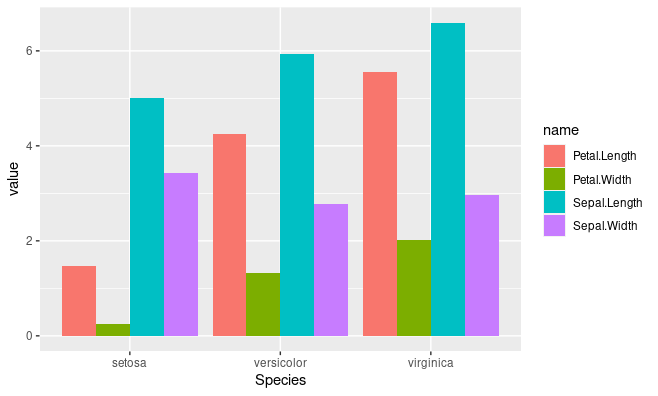
\includegraphics[width=5.20833in,height=\textheight]{images/08/Rplot01.png}

\textbf{Exercises}

5.5의 babies 데이터를 tidyverse 패키지를 활용하여 다시 분석해 보시오 (모든 경우를 tidyverse 패키지 함수를 사용할 필요는 없음, \texttt{select} 를 사용할 경우 \texttt{dplyr::select} 로 사용하시오)

\begin{enumerate}
\def\labelenumi{\arabic{enumi})}
\item
  babies 데이터의 변수를 확인하시오
\item
  babies 데이터의 id, age, gestation, wt, dwt, smoke 변수만을 갖는 newbabies 데이터를 만드시오
\item
  위 2번에 더해 999로 입력된 데이터를 제외한 newbabies 데이터를 만드시오
\item
  위 3번에 더해 smoke 데이터를 factor 형으로 변환한 smokef 변수를 추가한 newbabies 데이터를 만드시오
\item
  위 4번에 더해 25세 미만의 샘플만 갖고 smoke 변수는 제외한 는 newbabies 데이터를 만드시오
\end{enumerate}

\textbf{Exercises}

\begin{enumerate}
\def\labelenumi{\arabic{enumi}.}
\item
  \texttt{airquality} 데이터에서 \texttt{NA}가 포함된 샘플 (row)를 제거한 \texttt{myair} 라는 데이터셋을 생성하시오
\item
  위 1)에 Month 변수를 factor형으로 변환한 Monthf 를 추가하고 Month와 Day 변수를 제거한 새로운 데이터셋 \texttt{myair} 데이터를 생성하시오
\item
  myair 데이터에서 월별로 모든 변수에 (Ozone, Solar.R, Wind, Temp) 대한 평균을 구한 후 \texttt{myairmean} 변수에 저장하시오 (group\_by로 먼저 Monthf를 기준으로 grouping 필요, summarise\_all 사용)
\item
  위 3)에 더하여 데이터를 long 형으로 바꾸고 myairmean에 저장하시오
\item
  \texttt{ggplot}으로 myairmean 데이터의 월별 각 변수들의 평균 값들을 다음과 같은 bar 그래프로 그리시오
\end{enumerate}

\begin{verbatim}
ggplot(myairmean, aes(x=Monthf, y=value, fill=Monthf)) +
  geom_bar(stat="identity") +
  theme_bw()
\end{verbatim}

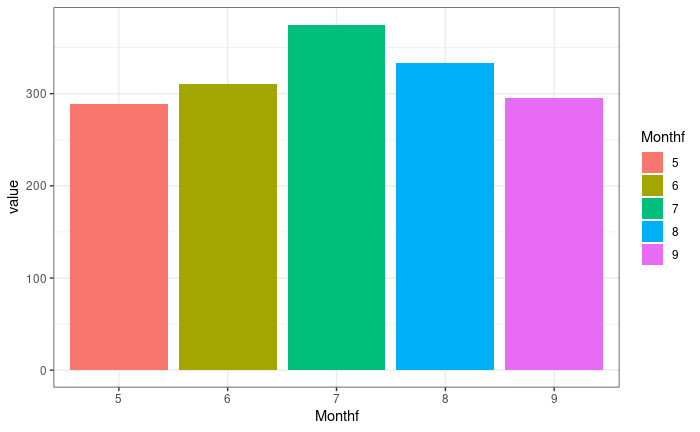
\includegraphics{images/08/00002e.png}

\textbf{Exercises}

InsectSprays 데이터는 살충제 6종에 대한 살충력을 (죽은 벌래의 마릿수) 나타내는 데이터이다. 각 살충제별로 평균과 표준편차를 구하시오

\textbf{Exercises}

dplyr 패키지의 starwars 는 스타워즈 영화에 나오는 등장인물들을 분석한 데이터셋 이다. 종족에 따른 키의 평균과 표준편차를 구하시오. (NA 데이터는 제외하고 분석)

\textbf{Exercises}

airquality 데이터는 뉴욕주의 몇몇 지점에서의 공기질을 측정한 데이터이다. 데이터에서 NA를 제거하고 각 월별로 평균 오존, 자외선, 풍속, 및 온도에 대한 평균과 표준편차를 구하시오

참고로 errorbar가 있는 막대그래프를 그려보겠습니다. 이를 위해서 먼저 두 테이블을 병합한 후 \texttt{ggplot2} 패키지의 \texttt{ggplot} 함수를 이용해서 그래프를 그립니다. 자세한 \texttt{ggplot}의 내용은 다음시간에 학습하겠습니다.

\begin{Shaded}
\begin{Highlighting}[]

\NormalTok{airdata }\OtherTok{\textless{}{-}} \FunctionTok{left\_join}\NormalTok{(airmean, airsd, }\AttributeTok{by=}\FunctionTok{c}\NormalTok{(}\StringTok{"Month"}\NormalTok{, }\StringTok{"name"}\NormalTok{))}

\FunctionTok{ggplot}\NormalTok{(airdata, }\FunctionTok{aes}\NormalTok{(}\AttributeTok{x=}\NormalTok{Month, }\AttributeTok{y=}\NormalTok{mean, }\AttributeTok{fill=}\NormalTok{name)) }\SpecialCharTok{+}
  \FunctionTok{geom\_bar}\NormalTok{(}\AttributeTok{stat=}\StringTok{"identity"}\NormalTok{, }\AttributeTok{position=}\StringTok{"dodge"}\NormalTok{) }\SpecialCharTok{+}
  \FunctionTok{geom\_errorbar}\NormalTok{(}\FunctionTok{aes}\NormalTok{(}\AttributeTok{ymin=}\NormalTok{mean}\SpecialCharTok{{-}}\NormalTok{sd, }\AttributeTok{ymax=}\NormalTok{mean}\SpecialCharTok{+}\NormalTok{sd), }\AttributeTok{position=}\FunctionTok{position\_dodge}\NormalTok{(}\AttributeTok{width=}\FloatTok{0.9}\NormalTok{), }\AttributeTok{width=}\FloatTok{0.4}\NormalTok{)}
\end{Highlighting}
\end{Shaded}

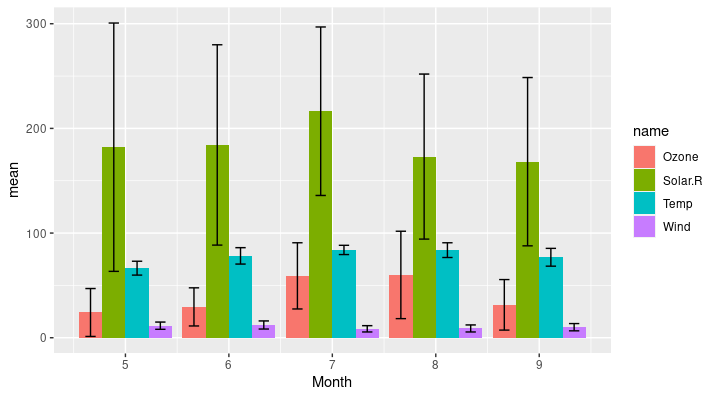
\includegraphics[width=5.20833in,height=\textheight]{images/08/Rplot02.png}

\textbf{Exercises}

\begin{enumerate}
\def\labelenumi{\arabic{enumi}.}
\tightlist
\item
  다음 코드를 이용해서 gse93819 실험 관련 파일들을 다운로드하여 저장하고 데이터의 구조 및 샘플들의 이름을 확인하시오
\end{enumerate}

\begin{verbatim}
myexp <- read.csv("https://github.com/greendaygh/kribbr2022/raw/main/examples/gse93819_expression_values.csv", header=T)
\end{verbatim}

\begin{enumerate}
\def\labelenumi{\arabic{enumi}.}
\setcounter{enumi}{1}
\item
  샘플들의 정보에 따라서 발현 데이터를 나누시오
\item
  각 그룹별 프루브들의 평균과 표준편차를 구하시오
\end{enumerate}

\textbf{Exercises}

gse103512 데이터도 동일한 방법으로 분석해 보시오

\hypertarget{uxcc38uxace0-uxd1b5uxacc4}{%
\section{참고 통계}\label{uxcc38uxace0-uxd1b5uxacc4}}

\begin{itemize}
\tightlist
\item
  \url{https://greendaygh.github.io/Rstat2020/statistical-inference.html\#two-sample-significance-tests}
\item
  정규분포와 t분포이해
\item
  t 통계량 계산
\item
  t-test 이해
\end{itemize}

\begin{center}\rule{0.5\linewidth}{0.5pt}\end{center}

이 저작물은 크리에이티브 커먼즈 저작자표시-비영리-변경금지 4.0 국제 라이선스에 따라 이용할 수 있습니다.

\hypertarget{data-visualization}{%
\chapter{Data visualization}\label{data-visualization}}

이번시간에는 \texttt{ggplot2}( \url{https://ggplot2.tidyverse.org/} )를 이용한 시각화에 대해서 알아봅니다. 데이터를 분석할 때 실제 데이터를 눈으로 확인하는 것은 중요합니다. raw 데이터를 보면서 크기 비교나 분포를 대략적으로 예측할 수 있다면 tool을 사용해서 나오는 결과를 가늠하는 척도가 될 수도 있습니다. \texttt{ggplot2} 는 Rstudio 개발팀의 해들리위컴이 (Hadley Wickham) 중심이 되어 만든 데이터 시각화 패키지입니다. 몇 가지 새로운 규칙을 학습해야 하지만 그 활용성이나 성능을 고려한다면 꼭 배워야할 패키지 중 하나입니다.

\hypertarget{basics}{%
\section{Basics}\label{basics}}

\texttt{iris} 데이터를 이용해서 간단하게 barplot을 그려봅니다. \texttt{iris} 데이터는 3가지 품종별 꽃잎과 꽃받침의 길이와 넓이를 측정한 데이터 입니다. 다음은 꽃잎의 길이와 넓이의 관계를 볼 수 있는 산점도 입니다.

\begin{Shaded}
\begin{Highlighting}[]
\FunctionTok{library}\NormalTok{(ggplot2)}
\FunctionTok{head}\NormalTok{(iris)}
\FunctionTok{str}\NormalTok{(iris)}
\FunctionTok{ggplot}\NormalTok{(}\AttributeTok{data=}\NormalTok{iris) }\SpecialCharTok{+}
  \FunctionTok{geom\_point}\NormalTok{(}\AttributeTok{mapping=}\FunctionTok{aes}\NormalTok{(}\AttributeTok{x=}\NormalTok{Petal.Length, }\AttributeTok{y=}\NormalTok{Petal.Width))}
\end{Highlighting}
\end{Shaded}

위에서는 두 개의 레이어가 있고 \texttt{ggplot}에서는 \texttt{+}를 이용해서 레이어들을 연결합니다. \texttt{ggplot()} 함수 뒤에 다양한 레이어들을 연결할 수 있고 \texttt{geom\_point()} 함수는 지정한 위치에 산점도 레이어를 추가하는 기능을 합니다. 각 레이어들은 다음과 같은 다양한 기능을 갖는 함수들로 구성될 수 있습니다.

\begin{itemize}
\tightlist
\item
  데이터 지정 (ggplot)
\item
  색상, 크기, x축의 값, y축의 값 등 심미적 요소 지정 (aes)
\item
  점, 선, 면 등 기하학적 요소 지정 (geoms)
\item
  그릴 통계량 지정 (stats)
\item
  테마, 스케일 지정 (theme)
\end{itemize}

일반적으로 \texttt{ggplot}을 이용하여 그래프를 그리는 순서는 다음과 같습니다.

\begin{itemize}
\tightlist
\item
  어떤 그래프를 그릴지 결정
\item
  ggplot의 데이터셋과 aesthetic 설정
\item
  geometric 요소와 적절한 statistics를 설정한 레이어 추가
\item
  스케일과 테마를 설정한 레이어 추가
\end{itemize}

ggplot만을 실행할 경우 데이터와 x, y 축만 지정한 상태로 어떤 그래프 (히스토그램인지, 산포도인지 등)를 그릴지 명시되어 있지 않아서 아무것도 그리지 않은 상태의 빈 켄버스만 그려지게 되며 \texttt{geom\_point()} 함수를 즉, 점을 그릴지 선을 그릴지 어떤 통계량을 그릴지 아니면 값 자체를 그릴지 등을 지정해 주고 나서야 비로서 그래프가 그려집니다.

\begin{Shaded}
\begin{Highlighting}[]
\FunctionTok{ggplot}\NormalTok{(}\AttributeTok{data=}\NormalTok{iris, }\AttributeTok{mapping=}\FunctionTok{aes}\NormalTok{(}\AttributeTok{x=}\NormalTok{Petal.Length, }\AttributeTok{y=}\NormalTok{Petal.Width))}
\NormalTok{?ggplot}
\FunctionTok{ggplot}\NormalTok{(iris, }\FunctionTok{aes}\NormalTok{(}\AttributeTok{x=}\NormalTok{Petal.Length, }\AttributeTok{y=}\NormalTok{Petal.Width))}
\FunctionTok{ggplot}\NormalTok{(iris, }\FunctionTok{aes}\NormalTok{(}\AttributeTok{x=}\NormalTok{Petal.Length, }\AttributeTok{y=}\NormalTok{Petal.Width)) }\SpecialCharTok{+} \FunctionTok{geom\_point}\NormalTok{()}
\end{Highlighting}
\end{Shaded}

\texttt{geom\_point()}의 도움말을 보면 다음과 같이 \texttt{data}, \texttt{mapping}, \texttt{stat} 등의 파라미터들이 있습니다. 이는 \texttt{ggplot}함수에서 설정한 \texttt{data}나 \texttt{mapping} 정보를 \texttt{geom\_point}에서 설정 하거나 완전히 다른 데이터를 x축과 y축에 그릴 수 있다는 뜻 이기도 합니다.

\begin{Shaded}
\begin{Highlighting}[]
\NormalTok{?geom\_point}
\FunctionTok{ggplot}\NormalTok{() }\SpecialCharTok{+} 
  \FunctionTok{geom\_point}\NormalTok{(}\AttributeTok{data=}\NormalTok{iris, }\AttributeTok{mapping=}\FunctionTok{aes}\NormalTok{(}\AttributeTok{x=}\NormalTok{Petal.Length, }\AttributeTok{y=}\NormalTok{Petal.Width)) }
\end{Highlighting}
\end{Shaded}

그런데 위 꽃잎의 길이와 넓이는 세 가지 다른 종류의 붓꽃에 대한 정보입니다. 따라서 각 종에 따라 다른 색이나 기호를 할당하는 것도 \texttt{mapping}에서 설정할 수 있습니다.

\begin{Shaded}
\begin{Highlighting}[]
\FunctionTok{ggplot}\NormalTok{(iris, }\FunctionTok{aes}\NormalTok{(}\AttributeTok{x=}\NormalTok{Petal.Length, }
                 \AttributeTok{y=}\NormalTok{Petal.Width, }
                 \AttributeTok{color=}\NormalTok{Species, }
                 \AttributeTok{shape=}\NormalTok{Species)) }\SpecialCharTok{+} 
  \FunctionTok{geom\_point}\NormalTok{()}

\FunctionTok{ggplot}\NormalTok{(iris, }\FunctionTok{aes}\NormalTok{(}\AttributeTok{x=}\NormalTok{Petal.Length, }\AttributeTok{y=}\NormalTok{Petal.Width)) }\SpecialCharTok{+} 
  \FunctionTok{geom\_point}\NormalTok{(}\FunctionTok{aes}\NormalTok{(}\AttributeTok{color=}\NormalTok{Species, }\AttributeTok{shape=}\NormalTok{Species))}
\end{Highlighting}
\end{Shaded}

위 산점도들의 \texttt{stat}은 \texttt{identity} 입니다. 즉, 따로 통계량을 계산할 필요 없이 값 그 자체를 사용하겠다는 것 입니다. 히스토그램의 경우 \texttt{geom\_bar()} 함수로 막대그래프를 그릴 수 있습니다. \texttt{geom\_bar}의 help페이지를 보면 \texttt{stat="count"}로 설정되어 있는 것을 알 수 있습니다. 꽃잎의 넓이에 대한 분포를 예로 구해봅니다. 히스토그램을 그릴경우 변수 한 개의 데이터만 필요하고 y축에는 자동으로 빈도수가 들어가게 되므로 \texttt{aes}에서 x만 mapping 해 주면 됩니다.

\begin{Shaded}
\begin{Highlighting}[]
\FunctionTok{ggplot}\NormalTok{(iris, }\FunctionTok{aes}\NormalTok{(}\AttributeTok{x=}\NormalTok{Petal.Width)) }\SpecialCharTok{+}  
  \FunctionTok{geom\_bar}\NormalTok{()}
\end{Highlighting}
\end{Shaded}

\hypertarget{bar-graph}{%
\section{Bar graph}\label{bar-graph}}

ggplot을 이용한 막대그래프 그리는 방법에 대해서 좀 더 알아보겠습니다. 앞서와 같이 ggplot 함수로 먼저 데이터와 aes로 x축 y축 등을 명시하고 \texttt{+} 오퍼레이터를 사용하여 필요한 레이어를 차례로 추가하면서 그래프를 그릴 수 있습니다. \texttt{geom\_bar()} 함수의 경우 x가 연속형일 경우는 아래와 같이 히스토그램을 그려주기 어렵습니다 (위 iris 예제에서 \texttt{geom\_bar()} 그래프에서는 실제 꽃받침의 width 값은 연속형이 맞으나 관측된 iris 데이터들이 같은 값들이 많은 범주형처럼 되어 있어 히스토그램 그림이 그려졌습니다) 이럴 경우 stat을 \texttt{bin}으로 바꿔주면 해당 범위 안에 있는 값들의 빈도수를 계산하여 히스토그램을 그릴 수 있습니다.

\begin{Shaded}
\begin{Highlighting}[]
\NormalTok{dat }\OtherTok{\textless{}{-}} \FunctionTok{data.frame}\NormalTok{(}\AttributeTok{x1=}\FunctionTok{rnorm}\NormalTok{(}\DecValTok{100}\NormalTok{))}
\FunctionTok{str}\NormalTok{(dat)}
\FunctionTok{ggplot}\NormalTok{(dat, }\FunctionTok{aes}\NormalTok{(}\AttributeTok{x=}\NormalTok{x1)) }\SpecialCharTok{+}
  \FunctionTok{geom\_bar}\NormalTok{()}

\FunctionTok{ggplot}\NormalTok{(dat, }\FunctionTok{aes}\NormalTok{(}\AttributeTok{x=}\NormalTok{x1)) }\SpecialCharTok{+}
  \FunctionTok{geom\_bar}\NormalTok{(}\AttributeTok{stat=}\StringTok{"bin"}\NormalTok{, }\AttributeTok{bins=}\DecValTok{30}\NormalTok{)}
\end{Highlighting}
\end{Shaded}

x가 이산형인 경우는 stat을 디폴트 값인 \texttt{count}로 설정하여 해당 값들의 빈도수를 그려줄 수 있습니다. 이는 앞서 \texttt{iris}에서 배운 예제와 같습니다.

\begin{Shaded}
\begin{Highlighting}[]
\NormalTok{x1 }\OtherTok{\textless{}{-}} \FunctionTok{sample}\NormalTok{(}\DecValTok{1}\SpecialCharTok{:}\DecValTok{4}\NormalTok{, }\DecValTok{100}\NormalTok{, }\AttributeTok{replace =}\NormalTok{ T)}
\NormalTok{dat }\OtherTok{\textless{}{-}} \FunctionTok{data.frame}\NormalTok{(}\AttributeTok{x=}\NormalTok{x1)}
\FunctionTok{ggplot}\NormalTok{(dat, }\FunctionTok{aes}\NormalTok{(}\AttributeTok{x=}\NormalTok{x)) }\SpecialCharTok{+}
  \FunctionTok{geom\_bar}\NormalTok{(}\AttributeTok{stat=}\StringTok{"count"}\NormalTok{)}
\end{Highlighting}
\end{Shaded}

이제 두 개의 변수가 있는 경우를 생각해 봅니다. 두 변수에 대해서 막대그래프를 그릴 경우 다음과 같이 \texttt{Error:\ stat\_count()\ must\ not\ be\ used\ with\ a\ y\ aesthetic.} 에러가 발생할 수 있습니다.

\begin{Shaded}
\begin{Highlighting}[]
\NormalTok{x1 }\OtherTok{\textless{}{-}} \FunctionTok{rnorm}\NormalTok{(}\DecValTok{10}\NormalTok{)}
\NormalTok{x2 }\OtherTok{\textless{}{-}} \FunctionTok{rnorm}\NormalTok{(}\DecValTok{10}\NormalTok{)}
\NormalTok{dat }\OtherTok{\textless{}{-}} \FunctionTok{data.frame}\NormalTok{(x1, x2)}
\FunctionTok{ggplot}\NormalTok{(dat, }\FunctionTok{aes}\NormalTok{(}\AttributeTok{x=}\NormalTok{x1, }\AttributeTok{y=}\NormalTok{x2)) }\SpecialCharTok{+}
  \FunctionTok{geom\_bar}\NormalTok{()}
\end{Highlighting}
\end{Shaded}

이는 \texttt{geom\_bar()}의 \texttt{stat}이 기본적으로 \texttt{count}로 설정되어 있으므로 생기는 에러 입니다. \texttt{stat}을 \texttt{identity}로 설정하면 x1값에 해당하는 x2값을 그려주는 막대 그래프를 그릴 수 있습니다. 참고로 이 그래프는 \texttt{geom\_point}와 비슷한 정보를 보여 주게 됩니다.

\begin{Shaded}
\begin{Highlighting}[]
\NormalTok{x1 }\OtherTok{\textless{}{-}} \FunctionTok{rnorm}\NormalTok{(}\DecValTok{10}\NormalTok{)}
\NormalTok{x2 }\OtherTok{\textless{}{-}} \FunctionTok{rnorm}\NormalTok{(}\DecValTok{10}\NormalTok{)}
\NormalTok{dat }\OtherTok{\textless{}{-}} \FunctionTok{data.frame}\NormalTok{(x1, x2)}
\FunctionTok{ggplot}\NormalTok{(dat, }\FunctionTok{aes}\NormalTok{(}\AttributeTok{x=}\NormalTok{x1, }\AttributeTok{y=}\NormalTok{x2)) }\SpecialCharTok{+}
  \FunctionTok{geom\_bar}\NormalTok{(}\AttributeTok{stat=}\StringTok{"identity"}\NormalTok{)}

\FunctionTok{ggplot}\NormalTok{(dat, }\FunctionTok{aes}\NormalTok{(}\AttributeTok{x=}\NormalTok{x1, }\AttributeTok{y=}\NormalTok{x2)) }\SpecialCharTok{+}
  \FunctionTok{geom\_point}\NormalTok{()}
\end{Highlighting}
\end{Shaded}

다음과 같이 레이어를 추가하여 두 그래프를 같은 화면에 그릴 수도 있습니다. 여기서 \texttt{col}과 \texttt{size}는 \texttt{aes}함수안에서 쓰이지 않았음을 주의하시기 바랍니다. \texttt{aes}에서는 데이터와 특정 모양, 색깔을 mapping 해주는 역할을 하고 아래와 같이 지정해 줄 경우 데이터와 상관 없이 해당 레이어의 모든 그래프에 대해서 일괄적으로 적용되게 됩니다.

\begin{Shaded}
\begin{Highlighting}[]
\FunctionTok{ggplot}\NormalTok{(dat, }\FunctionTok{aes}\NormalTok{(}\AttributeTok{x=}\NormalTok{x1, }\AttributeTok{y=}\NormalTok{x2)) }\SpecialCharTok{+}
  \FunctionTok{geom\_bar}\NormalTok{(}\AttributeTok{stat=}\StringTok{"identity"}\NormalTok{) }\SpecialCharTok{+}
  \FunctionTok{geom\_point}\NormalTok{(}\FunctionTok{aes}\NormalTok{(}\AttributeTok{col=}\StringTok{"red"}\NormalTok{, }\AttributeTok{size=}\DecValTok{5}\NormalTok{))}
\NormalTok{?geom\_point}
\end{Highlighting}
\end{Shaded}

또한 다음과 같이 다양한 레이어를 추가하여 필요한 기능을 사용할 수 있습니다. \texttt{fill=x1} 이라는 코드는 막대그래프의 색을 채울 때 x1에 따라서 다른 값들을 채우는 역할을 한다고 보면 되겠습니다.

\begin{Shaded}
\begin{Highlighting}[]
\NormalTok{x1 }\OtherTok{\textless{}{-}} \FunctionTok{as.factor}\NormalTok{(}\DecValTok{1}\SpecialCharTok{:}\DecValTok{3}\NormalTok{)}
\NormalTok{y1 }\OtherTok{\textless{}{-}} \FunctionTok{tabulate}\NormalTok{(}\FunctionTok{sample}\NormalTok{(x1, }\DecValTok{100}\NormalTok{, }\AttributeTok{replace=}\NormalTok{T))}
\NormalTok{dat }\OtherTok{\textless{}{-}} \FunctionTok{data.frame}\NormalTok{(x1, y1)}
\FunctionTok{ggplot}\NormalTok{(dat, }\FunctionTok{aes}\NormalTok{(}\AttributeTok{x=}\NormalTok{x1, }\AttributeTok{y=}\NormalTok{y1, }\AttributeTok{fill=}\NormalTok{x1)) }\SpecialCharTok{+}
  \FunctionTok{geom\_bar}\NormalTok{(}\AttributeTok{stat=}\StringTok{"identity"}\NormalTok{) }
\end{Highlighting}
\end{Shaded}

위 그래프에 더해서 legend를 없애고 x, y축 라벨과 스케일, 그리고 타이틀 등을 설정할 수 있습니다.

\begin{Shaded}
\begin{Highlighting}[]
\FunctionTok{ggplot}\NormalTok{(dat, }\FunctionTok{aes}\NormalTok{(}\AttributeTok{x=}\NormalTok{x1, }\AttributeTok{y=}\NormalTok{y1, }\AttributeTok{fill=}\NormalTok{x1)) }\SpecialCharTok{+}
  \FunctionTok{geom\_bar}\NormalTok{(}\AttributeTok{stat=}\StringTok{"identity"}\NormalTok{) }\SpecialCharTok{+}
  \FunctionTok{guides}\NormalTok{(}\AttributeTok{fill=}\ConstantTok{FALSE}\NormalTok{) }\SpecialCharTok{+}
  \FunctionTok{xlab}\NormalTok{(}\StringTok{"Discrete cases"}\NormalTok{) }\SpecialCharTok{+} 
  \FunctionTok{ylab}\NormalTok{(}\StringTok{"Value"}\NormalTok{) }\SpecialCharTok{+}
  \FunctionTok{ylim}\NormalTok{(}\FunctionTok{c}\NormalTok{(}\DecValTok{0}\NormalTok{,}\DecValTok{50}\NormalTok{))}\SpecialCharTok{+}
  \FunctionTok{ggtitle}\NormalTok{(}\StringTok{"Bar graph for x:discrete and y:value"}\NormalTok{)}
\end{Highlighting}
\end{Shaded}

\textbf{Exercises (revisit) }

\begin{itemize}
\tightlist
\item
  목적: 그룹별로 발현이 다른 유전자 탐색
\end{itemize}

\begin{enumerate}
\def\labelenumi{\arabic{enumi}.}
\tightlist
\item
  다음 코드를 이용해서 gse93819 실험 관련 파일들을 다운로드하여 저장하고 데이터의 구조 및 샘플들의 이름을 확인하시오
\end{enumerate}

\begin{Shaded}
\begin{Highlighting}[]
\NormalTok{myexp }\OtherTok{\textless{}{-}} \FunctionTok{read.csv}\NormalTok{(}\StringTok{"https://github.com/greendaygh/kribbr2022/raw/main/examples/gse93819\_expression\_values.csv"}\NormalTok{, }\AttributeTok{header=}\NormalTok{T)}
\NormalTok{myexp}
\end{Highlighting}
\end{Shaded}

\begin{enumerate}
\def\labelenumi{\arabic{enumi}.}
\setcounter{enumi}{1}
\item
  샘플들의 정보에 따라서 (그룹별로) 발현 데이터를 나누시오 (필요하지 않을 수 있음)
\item
  각 그룹별 프루브들의 평균과 표준편차를 구하시오
\end{enumerate}

\begin{itemize}
\tightlist
\item
  분석 목적에 따른 샘플, 변수, 값 구분하기
\item
  평균을 구할 때 샘플의 특정 변수에 대한 평균을 구함
\item
  발현 데이터와 메타데이터 두 개의 테이블로 만들어 작업
\end{itemize}

\begin{Shaded}
\begin{Highlighting}[]
\FunctionTok{require}\NormalTok{(knitr)}
\FunctionTok{require}\NormalTok{(kableExtra)}

\NormalTok{mytable }\OtherTok{\textless{}{-}}\NormalTok{ myexp[}\DecValTok{1}\SpecialCharTok{:}\DecValTok{4}\NormalTok{, }\DecValTok{1}\SpecialCharTok{:}\DecValTok{4}\NormalTok{]}
\NormalTok{mytable }

\NormalTok{mytablet }\OtherTok{\textless{}{-}} \FunctionTok{data.frame}\NormalTok{(}\FunctionTok{t}\NormalTok{(myexp[}\DecValTok{1}\SpecialCharTok{:}\DecValTok{4}\NormalTok{, }\DecValTok{1}\SpecialCharTok{:}\DecValTok{4}\NormalTok{]))}
\NormalTok{mytablet }
\end{Highlighting}
\end{Shaded}

\begin{enumerate}
\def\labelenumi{\arabic{enumi}.}
\setcounter{enumi}{3}
\tightlist
\item
  각 프루브의 평균값을 bargraph로 그리고 표준편차로 에러바를 그리시오
\end{enumerate}

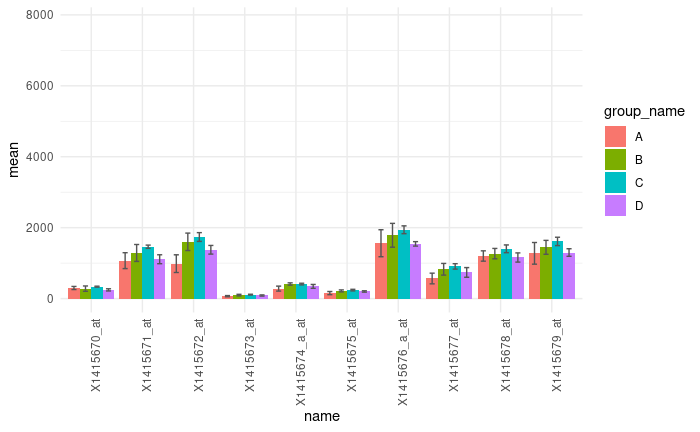
\includegraphics[width=4.16667in,height=\textheight]{images/07/barploterrorbar.png}

\hypertarget{line-graph}{%
\section{Line graph}\label{line-graph}}

다음으로 ggplot을 이용한 line graph를 그리는 방법을 알아 봅니다. Line graph는 geom\_line이라는 함수를 사용해서 그릴 수 있으며 stat의 사용법은 앞서 bar graph와 같습니다.

\begin{Shaded}
\begin{Highlighting}[]
\NormalTok{x1 }\OtherTok{\textless{}{-}} \FunctionTok{c}\NormalTok{(}\DecValTok{12}\NormalTok{, }\DecValTok{21}\NormalTok{, }\DecValTok{40}\NormalTok{)}
\NormalTok{x2 }\OtherTok{\textless{}{-}} \FunctionTok{c}\NormalTok{(}\DecValTok{33}\NormalTok{, }\DecValTok{10}\NormalTok{, }\DecValTok{82}\NormalTok{)}
\NormalTok{dat }\OtherTok{\textless{}{-}} \FunctionTok{data.frame}\NormalTok{(x1, x2)}
\FunctionTok{ggplot}\NormalTok{(dat, }\FunctionTok{aes}\NormalTok{(}\AttributeTok{x=}\NormalTok{x1, }\AttributeTok{y=}\NormalTok{x2)) }\SpecialCharTok{+}
  \FunctionTok{geom\_line}\NormalTok{()}
\end{Highlighting}
\end{Shaded}

아래와 같이 그려지는 선의 두께를 조절하거나 레이어를 추가하는 방법으로 점을 추가로 그려볼 수 있습니다. \texttt{fill}의 경우 특정 도형에 채워지는 색을 의미합니다. 도형에 대한 자세한 종류는 \texttt{?pch} 라는 도움말로 살펴보실 수 있습니다.

\begin{Shaded}
\begin{Highlighting}[]
\FunctionTok{ggplot}\NormalTok{(dat, }\FunctionTok{aes}\NormalTok{(}\AttributeTok{x=}\NormalTok{x1, }\AttributeTok{y=}\NormalTok{x2)) }\SpecialCharTok{+}
  \FunctionTok{geom\_line}\NormalTok{(}\AttributeTok{size=}\DecValTok{2}\NormalTok{) }\SpecialCharTok{+}
  \FunctionTok{geom\_point}\NormalTok{(}\AttributeTok{size=}\DecValTok{4}\NormalTok{, }\AttributeTok{pch=}\DecValTok{21}\NormalTok{, }\AttributeTok{fill=}\StringTok{"white"}\NormalTok{) }\SpecialCharTok{+}
  \FunctionTok{guides}\NormalTok{(}\AttributeTok{fill=}\ConstantTok{FALSE}\NormalTok{) }\SpecialCharTok{+}
  \FunctionTok{ylim}\NormalTok{(}\FunctionTok{c}\NormalTok{(}\DecValTok{0}\NormalTok{, }\DecValTok{100}\NormalTok{)) }\SpecialCharTok{+}
  \FunctionTok{xlab}\NormalTok{(}\StringTok{"Continuous cases"}\NormalTok{) }\SpecialCharTok{+} \FunctionTok{ylab}\NormalTok{(}\StringTok{"Value"}\NormalTok{) }\SpecialCharTok{+}
  \FunctionTok{ggtitle}\NormalTok{(}\StringTok{"Line graph for x:continuous and y:continuous"}\NormalTok{)}
\end{Highlighting}
\end{Shaded}

위 경우는 x와 y가 모두 연속형 데이터일 경우 입니다. x는 이산형, y가 연속형일 경우 일반적으로 bar graph를 이용하여 그래프를 그리게 됩니다. 그런데 이런 bar의 높이에 해당하는 값들을 서로 선으로 연결하고 싶은 경우가 있습니다.

\begin{Shaded}
\begin{Highlighting}[]
\NormalTok{x1 }\OtherTok{\textless{}{-}} \FunctionTok{as.factor}\NormalTok{(}\FunctionTok{c}\NormalTok{(}\DecValTok{1}\SpecialCharTok{:}\DecValTok{3}\NormalTok{))}
\NormalTok{y1 }\OtherTok{\textless{}{-}} \FunctionTok{c}\NormalTok{(}\DecValTok{33}\NormalTok{, }\DecValTok{10}\NormalTok{, }\DecValTok{82}\NormalTok{)}
\NormalTok{dat }\OtherTok{\textless{}{-}} \FunctionTok{data.frame}\NormalTok{(x1, y1)}
\FunctionTok{str}\NormalTok{(dat)}
\FunctionTok{ggplot}\NormalTok{(dat, }\FunctionTok{aes}\NormalTok{(}\AttributeTok{x=}\NormalTok{x1, }\AttributeTok{y=}\NormalTok{y1)) }\SpecialCharTok{+}
  \FunctionTok{geom\_bar}\NormalTok{(}\AttributeTok{stat=}\StringTok{"identity"}\NormalTok{) }\SpecialCharTok{+}
  \FunctionTok{xlab}\NormalTok{(}\StringTok{"Discrete cases"}\NormalTok{) }\SpecialCharTok{+} \FunctionTok{ylab}\NormalTok{(}\StringTok{"Value"}\NormalTok{) }\SpecialCharTok{+}
  \FunctionTok{ylim}\NormalTok{(}\FunctionTok{c}\NormalTok{(}\DecValTok{0}\NormalTok{,}\DecValTok{100}\NormalTok{))}\SpecialCharTok{+}
  \FunctionTok{ggtitle}\NormalTok{(}\StringTok{"Line plot for x:discrete and y:continuous"}\NormalTok{)}
\end{Highlighting}
\end{Shaded}

이 때는 다음과 같이 \texttt{aes}의 \texttt{group} 이라는 파라미터를 설정하여 두 점 이상을 연결할 수 있습니다. 만약 group으로 나타낼 수 있는 변수가 없을 경우 \texttt{group=1}이라고 명시해 주고 선을 그릴 수 있으며 이 경우 모든 값들이 같은 \texttt{1} 그룹에 있는 것으로 간주됩니다. \texttt{1}이라는 것은 하나의 예이며 어떤 숫자나 문자가 와도 괜찮습니다.

\begin{Shaded}
\begin{Highlighting}[]
\FunctionTok{ggplot}\NormalTok{(dat, }\FunctionTok{aes}\NormalTok{(}\AttributeTok{x=}\NormalTok{x1, }\AttributeTok{y=}\NormalTok{y1, }\AttributeTok{group=}\DecValTok{1}\NormalTok{)) }\SpecialCharTok{+}
  \FunctionTok{geom\_bar}\NormalTok{(}\AttributeTok{stat=}\StringTok{"identity"}\NormalTok{) }\SpecialCharTok{+}
  \FunctionTok{geom\_line}\NormalTok{() }\SpecialCharTok{+}
  \FunctionTok{xlab}\NormalTok{(}\StringTok{"Discrete cases"}\NormalTok{) }\SpecialCharTok{+} \FunctionTok{ylab}\NormalTok{(}\StringTok{"Value"}\NormalTok{) }\SpecialCharTok{+}
  \FunctionTok{ylim}\NormalTok{(}\FunctionTok{c}\NormalTok{(}\DecValTok{0}\NormalTok{,}\DecValTok{100}\NormalTok{))}\SpecialCharTok{+}
  \FunctionTok{ggtitle}\NormalTok{(}\StringTok{"Line plot for x:discrete and y:continuous"}\NormalTok{)}
\end{Highlighting}
\end{Shaded}

위에서와 같은 방법으로 point와 bar 등을 같이 그려줄 수 있습니다.

\begin{Shaded}
\begin{Highlighting}[]
\FunctionTok{ggplot}\NormalTok{(dat, }\FunctionTok{aes}\NormalTok{(}\AttributeTok{x=}\NormalTok{x1, }\AttributeTok{y=}\NormalTok{y1, }\AttributeTok{group=}\DecValTok{1}\NormalTok{)) }\SpecialCharTok{+}
  \FunctionTok{geom\_bar}\NormalTok{(}\FunctionTok{aes}\NormalTok{(}\AttributeTok{fill=}\NormalTok{x1), }\AttributeTok{stat=}\StringTok{"identity"}\NormalTok{) }\SpecialCharTok{+}
  \FunctionTok{geom\_line}\NormalTok{(}\AttributeTok{size=}\DecValTok{2}\NormalTok{, }\AttributeTok{color=}\StringTok{"gray"}\NormalTok{) }\SpecialCharTok{+}
  \FunctionTok{geom\_point}\NormalTok{(}\AttributeTok{size=}\DecValTok{4}\NormalTok{, }\AttributeTok{pch=}\DecValTok{21}\NormalTok{, }\AttributeTok{fill=}\StringTok{"white"}\NormalTok{) }\SpecialCharTok{+}
  \FunctionTok{xlab}\NormalTok{(}\StringTok{"Discrete cases"}\NormalTok{) }\SpecialCharTok{+} \FunctionTok{ylab}\NormalTok{(}\StringTok{"Value"}\NormalTok{) }\SpecialCharTok{+}
  \FunctionTok{ylim}\NormalTok{(}\FunctionTok{c}\NormalTok{(}\DecValTok{0}\NormalTok{,}\DecValTok{100}\NormalTok{))}\SpecialCharTok{+}
  \FunctionTok{ggtitle}\NormalTok{(}\StringTok{"Line for x:discrete and y:value"}\NormalTok{)}
\end{Highlighting}
\end{Shaded}

여기서는 fill 옵션이 geom\_bar에 하나 geom\_point에 하나씩 쓰였는데 geom\_bar에서 사용된 fill은 bar에 채워지는 색을 x1의 값에 따라 바꾸겠다는 것을 의미하고 (aes함수 안에 사용) \texttt{geom\_point}의 fill은 데이터에 상관 없이 모두 white로 채우라는 명령 입니다. 각 geometry에 따라서 필요한 옵션이 다르므로 각각의 geom\_xxx를 사용할 때 상황에 맞게 사용하시면 되겠습니다.

\hypertarget{smoothing}{%
\section{Smoothing}\label{smoothing}}

산포도는 앞서와 같이 데이터를 점으로 표현한 그래프입니다. Smoothing은 관측된 데이터를 이용하여 모형을 추정하는데 사용되는 통계적 방법이며 이를 그래프로 표현하여 추세선을 그릴 수 있습니다. 예를 들어 몸무게와 키라는 두 변수의 관계를 알아보고자 할 때 산포도를 그리고 Smoothing을 통해 점들의 평균값을 이어주는 방법으로 모형을 추정하고 추세선을 그릴 수 있습니다.

\texttt{mtcars} 데이터는 1974년 미국 자동차 잡지에서 추출한 데이터로서 당시 다양한 모델의 자동차에대한 성능을 저장하고 있습니다 (\texttt{?mtcars}로 자세한 정보를 볼 수 있음). 이 데이터를 이용해서 연비와 마력 (horsepower) 두 변수의 관계를 그래프로 그려보겠습니다. 직관적으로 생각하면 두 변수는 반비례 할 것으로 기대됩니다. \texttt{ggplot}을 활용해서 두 변수의 산포도를 그리고 smoothing을 수행해 보도록 하겠습니다.

\begin{Shaded}
\begin{Highlighting}[]
\FunctionTok{ggplot}\NormalTok{(mtcars, }\FunctionTok{aes}\NormalTok{(}\AttributeTok{x=}\NormalTok{mpg, }\AttributeTok{y=}\NormalTok{hp)) }\SpecialCharTok{+}
  \FunctionTok{geom\_point}\NormalTok{()}
\end{Highlighting}
\end{Shaded}

위와 같이 \texttt{mtcars}는 \texttt{data.frame}이므로 \texttt{ggplot}으로 바로 받아서 x축과 y축 mapping에 필요한 변수들 이름을 직접 할당하고 \texttt{geom\_point}함수를 이용해서 간단히 산포도를 그릴 수 있습니다. 이 산포도만으로도 mpg와 hp 두 변수간의 관계가 역함수 관계임을 알 수 있고 또한 선형이 아닌 것도 알 수 있습니다. 이제 위 그림에 \texttt{geom\_smooth()}함수를 이용해서 (모형) 적합 곡선 (또는 추세선)을 그려봅니다.

\begin{Shaded}
\begin{Highlighting}[]
\FunctionTok{ggplot}\NormalTok{(mtcars, }\FunctionTok{aes}\NormalTok{(}\AttributeTok{x=}\NormalTok{mpg, }\AttributeTok{y=}\NormalTok{hp)) }\SpecialCharTok{+}
  \FunctionTok{geom\_point}\NormalTok{() }\SpecialCharTok{+}
  \FunctionTok{geom\_smooth}\NormalTok{()}
\end{Highlighting}
\end{Shaded}

간단히 \texttt{geom\_smooth()} 한 줄을 추가하여 추세선을 그렸으며 경고 메세지에서 볼 수 있듯이 알고리즘은 \texttt{loess} 모형을 사용했고 공식은 (formula는) \texttt{y\textasciitilde{}x}로, 즉, y축 변수를 반응변수로 x축 변수를 설명변수로 설정하여 그려졌습니다. 직선의 공식 \texttt{y=ax+b}를 생각해 보시면 무슨 의미인지 이해가 더 쉬울듯 합니다. \texttt{?geom\_smooth}로 보면 알 수 있듯이 모형을 적합하는 알고리즘 옵션을 \texttt{lm}, \texttt{glm}, \texttt{loess} 등 다양하게 설정할 수 있으며 \texttt{auto}로 하게 되면 데이터의 크기나 형식에 맞춰서 방법을 자동으로 선택해서 그려주게 됩니다. \texttt{se} 옵션은 기본적으로 \texttt{TRUE} 값을 가지며 위 그림에서 볼 수 있는 선분 주위의 회색 구간으로 신뢰구간을 그려주는 옵션 입니다. \texttt{span} 옵션은 loess 모형의 smoothing 정도를 조절할 수 있는데 이는 직접 바꿔가면서 실습을 해보면 이해에 도움이 되겠습니다.

\begin{Shaded}
\begin{Highlighting}[]
\FunctionTok{ggplot}\NormalTok{(mtcars, }\FunctionTok{aes}\NormalTok{(}\AttributeTok{x=}\NormalTok{mpg, }\AttributeTok{y=}\NormalTok{hp)) }\SpecialCharTok{+}
  \FunctionTok{geom\_point}\NormalTok{() }\SpecialCharTok{+}
  \FunctionTok{geom\_smooth}\NormalTok{(}\AttributeTok{se=}\ConstantTok{FALSE}\NormalTok{, }\AttributeTok{span=}\FloatTok{0.2}\NormalTok{)}
\end{Highlighting}
\end{Shaded}

위와 같이 \texttt{span} 옵션을 작게 설정할 수록 관측된 데이터(점)에 선분(모형)이 가까이 붙게 됩니다. 이를 과대적합 (overfitting)이라고 하며 간단히 설명하면 관측된 데이터에만 너무 잘맞는 모형을 만드는 경우를 말합니다. 이럴 경우 새롭게 관측된 데이터는 모형의 예측값과 잘 맞지 않게 됩니다.

이번에는 모의 데이터를 생성해서 그래프를 그려보겠습니다. 네 개 학급에 있는 학생들의 키와 몸무게를 저장한 데이터를 만들어 봅니다. 이 경우 몇 개의 변수가 필요할지 생각해 보시기 바랍니다. 키와 몸무게 그리고 학급을 나타내는 변수 3개가 필요하며 키와 몸무게는 정수형, 그룹을 나타내는 변수는 문자형이나 factor형으로 나타내면 되겠습니다. 각 학급의 학생수는 50명으로 총 200명의 학생이 있는 것으로 하며 각 그룹별로 키나 몸무게의 차이는 없고 키가 큰 사람은 몸무게가 많이 나가는 것으로 합니다. 키와 몸무게 사이에는 다음과 같은 연관성을 만들어 줍니다. \(height= weight + N(100, 10)\)

\begin{Shaded}
\begin{Highlighting}[]
\NormalTok{weights }\OtherTok{\textless{}{-}} \FunctionTok{rnorm}\NormalTok{(}\DecValTok{200}\NormalTok{, }\DecValTok{75}\NormalTok{, }\DecValTok{5}\NormalTok{)}
\NormalTok{heights }\OtherTok{\textless{}{-}}\NormalTok{ weights }\SpecialCharTok{+} \FunctionTok{rnorm}\NormalTok{(}\DecValTok{200}\NormalTok{, }\DecValTok{100}\NormalTok{, }\DecValTok{5}\NormalTok{)}
\NormalTok{classes }\OtherTok{\textless{}{-}} \FunctionTok{sample}\NormalTok{(}\FunctionTok{c}\NormalTok{(}\StringTok{"A"}\NormalTok{, }\StringTok{"B"}\NormalTok{, }\StringTok{"C"}\NormalTok{, }\StringTok{"D"}\NormalTok{), }\AttributeTok{size=}\FunctionTok{length}\NormalTok{(heights), }\AttributeTok{replace =}\NormalTok{ T)}
\NormalTok{mydata }\OtherTok{\textless{}{-}} \FunctionTok{data.frame}\NormalTok{(heights, weights, classes)}
\FunctionTok{str}\NormalTok{(mydata)}
\end{Highlighting}
\end{Shaded}

이제 위 데이터를 이용해서 몸무게와 키의 산포도와 추세선을 그려보고 추가로 그룹별로 다른 색의 점으로 표현해 보겠습니다.

\begin{Shaded}
\begin{Highlighting}[]
\FunctionTok{ggplot}\NormalTok{(mydata, }\FunctionTok{aes}\NormalTok{(}\AttributeTok{x=}\NormalTok{weights, }\AttributeTok{y=}\NormalTok{heights, }\AttributeTok{color=}\NormalTok{classes)) }\SpecialCharTok{+}
  \FunctionTok{geom\_point}\NormalTok{() }\SpecialCharTok{+}
  \FunctionTok{geom\_smooth}\NormalTok{()}
\end{Highlighting}
\end{Shaded}

그런데 위와 같은 코드를 실행하면 그룹마다 다른 점과 smooth 선분이 그려집니다. 우리가 원하는 그림은 단지 점만 그룹별로 다른 색으로 표현하고 추세선은 전체 학생들에 대해서 하나의 선분만 그려지길 원합니다. 이제 우리가 알아야할 부분은 각 레이어마다 mapping을 지정할 수 있다는 것이고 이 원리를 이해한다면 다음과 같이 \texttt{geom\_point}에서는 \texttt{color}를 mapping해 주고 \texttt{geom\_smooth}에서는 지정해주지 않으면 됩니다.

\begin{Shaded}
\begin{Highlighting}[]
\FunctionTok{ggplot}\NormalTok{(mydata) }\SpecialCharTok{+}
  \FunctionTok{geom\_point}\NormalTok{(}\FunctionTok{aes}\NormalTok{(}\AttributeTok{x=}\NormalTok{weights, }\AttributeTok{y=}\NormalTok{heights, }\AttributeTok{color=}\NormalTok{classes)) }\SpecialCharTok{+}
  \FunctionTok{geom\_smooth}\NormalTok{(}\FunctionTok{aes}\NormalTok{(}\AttributeTok{x=}\NormalTok{weights, }\AttributeTok{y=}\NormalTok{heights))}
\end{Highlighting}
\end{Shaded}

그리고 중복되는 부분을 줄여줄 수도 있습니다. 즉, ggplot에서 지정하는 mapping은 하위 layer에 모두 적용이 되며 각 layer마다 다른 mapping 특성을 부여하고 싶을 경우 해당 layer의 mapping 함수 (aes)를 이용하여 설정할 수 있다는 점을 기억하시기 바랍니다.

\begin{Shaded}
\begin{Highlighting}[]
\FunctionTok{ggplot}\NormalTok{(mydata, }\FunctionTok{aes}\NormalTok{(}\AttributeTok{x=}\NormalTok{weights, }\AttributeTok{y=}\NormalTok{heights)) }\SpecialCharTok{+}
  \FunctionTok{geom\_point}\NormalTok{(}\FunctionTok{aes}\NormalTok{(}\AttributeTok{color=}\NormalTok{classes)) }\SpecialCharTok{+}
  \FunctionTok{geom\_smooth}\NormalTok{()}
\end{Highlighting}
\end{Shaded}

\hypertarget{statstics-and-positions}{%
\section{Statstics and positions}\label{statstics-and-positions}}

앞서 smoothing 곡선은 실제 데이터에서 관측된 값이 아닌 계산된 값을 그래프에 표현한 것 입니다. 막대그래프에서도 y축 count 값은 관측된 값이 아닌 빈도수를 계산한 값이고 boxplot의 경우도 중간값 1,3사분위수 등 통계량을 표현해 주는 그래프 입니다. 이는 대부분 통계 분석용 소프트웨어에서 제공되는 기능으로 통계량을 가시화 해주는 역할을 합니다. \texttt{ggplot2}에서도 각 geom 레이어에 \texttt{stat}이라는 옵션을 통해 이러한 통계량을 그래프로 표현할 수 있습니다. 예를 들어 앞서 생성한 키, 몸무게 데이터에서 키의 분포를 보기 위한 히스토그램을 그리면 \texttt{geom\_histogram}을 사용할 수 있고 이 레이어의 \texttt{stat} 옵션의 기본값은 \texttt{"bin"} 입니다 (\texttt{?geom\_histogram} 참고).

\begin{Shaded}
\begin{Highlighting}[]
\FunctionTok{library}\NormalTok{(tidyverse)}

\NormalTok{weights }\OtherTok{\textless{}{-}} \FunctionTok{rnorm}\NormalTok{(}\DecValTok{200}\NormalTok{, }\DecValTok{75}\NormalTok{, }\DecValTok{5}\NormalTok{)}
\NormalTok{heights }\OtherTok{\textless{}{-}}\NormalTok{ weights }\SpecialCharTok{+} \FunctionTok{rnorm}\NormalTok{(}\DecValTok{200}\NormalTok{, }\DecValTok{100}\NormalTok{, }\DecValTok{5}\NormalTok{)}
\NormalTok{classes }\OtherTok{\textless{}{-}} \FunctionTok{sample}\NormalTok{(}\FunctionTok{c}\NormalTok{(}\StringTok{"A"}\NormalTok{, }\StringTok{"B"}\NormalTok{, }\StringTok{"C"}\NormalTok{, }\StringTok{"D"}\NormalTok{), }\AttributeTok{size=}\FunctionTok{length}\NormalTok{(heights), }\AttributeTok{replace =}\NormalTok{ T)}
\NormalTok{mydata }\OtherTok{\textless{}{-}} \FunctionTok{data.frame}\NormalTok{(heights, weights, classes)}
\FunctionTok{str}\NormalTok{(mydata)}

\FunctionTok{ggplot}\NormalTok{(mydata, }\FunctionTok{aes}\NormalTok{(}\AttributeTok{x=}\NormalTok{heights)) }\SpecialCharTok{+}
  \FunctionTok{geom\_histogram}\NormalTok{()}
\end{Highlighting}
\end{Shaded}

경고 문구의 \texttt{bins=30}은 기본 \texttt{stat}옵션이 \texttt{bin}인데 \texttt{bins}옵션은 null로 되어 있기 때문에 경고가 발생한 것이고 30으로 강제 할당해서 그린다는 메세지 입니다. bins 옵션을 다르게 해서 테스트 해보시기 바랍니다. 또한 \texttt{stat="identity"}로 그래프를 그린 경우는 데이터 값을 그대로 그린다는 것도 다시 기억해 보시기 바랍니다.

\begin{Shaded}
\begin{Highlighting}[]
\FunctionTok{ggplot}\NormalTok{(mydata, }\FunctionTok{aes}\NormalTok{(}\AttributeTok{x=}\NormalTok{heights)) }\SpecialCharTok{+}
  \FunctionTok{geom\_histogram}\NormalTok{(}\AttributeTok{stat=}\StringTok{"identity"}\NormalTok{)}

\FunctionTok{ggplot}\NormalTok{(mydata, }\FunctionTok{aes}\NormalTok{(}\AttributeTok{x=}\NormalTok{heights, }\AttributeTok{y=}\NormalTok{weights)) }\SpecialCharTok{+}
  \FunctionTok{geom\_histogram}\NormalTok{(}\AttributeTok{stat=}\StringTok{"identity"}\NormalTok{)}
\end{Highlighting}
\end{Shaded}

또 다른 예를위해 앞서 키 몸무게 데이터에 혈액형 변수를 추가해 보겠습니다. 혈액형은 위 4개 학급에 관계 없이 A, B, O, AB 네 그룹으로 나눌 수 있으며 200명의 학생들에게 랜덤하게 할당하도록 합니다.

\begin{Shaded}
\begin{Highlighting}[]
\NormalTok{bloodtype }\OtherTok{\textless{}{-}} \FunctionTok{sample}\NormalTok{(}\FunctionTok{c}\NormalTok{(}\StringTok{"A"}\NormalTok{, }\StringTok{"B"}\NormalTok{, }\StringTok{"O"}\NormalTok{, }\StringTok{"AB"}\NormalTok{), }\FunctionTok{nrow}\NormalTok{(mydata), }\AttributeTok{replace=}\NormalTok{T)}
\NormalTok{mynewdata }\OtherTok{\textless{}{-}} \FunctionTok{data.frame}\NormalTok{(mydata, bloodtype)}
\FunctionTok{str}\NormalTok{(mynewdata)}
\end{Highlighting}
\end{Shaded}

위와 같이 새로운 변수 bloodtype 이 \texttt{factor}형으로 추가되어 새로운 \texttt{data.frame}을 생성하도록 했습니다. 이제 각 학급별로 몇 명의 혈액형 타입을 갖는 학생들이 있는지를 막대그래프로 표현해 보도록 하겠습니다. 혈액형의 타입별로 다른 색으로 막대를 칠하도록 해봅니다. 막대그래프의 색은 \texttt{fill}옵션으로 채울수 있고 막대그래프는 \texttt{geom\_bar}그리고 이 레이어의 \texttt{stat}은 기본값이 \texttt{count}이므로 따로 명시하지 않은채로 다음과 같이 코드를 작성할 수 있습니다.

\begin{Shaded}
\begin{Highlighting}[]
\FunctionTok{ggplot}\NormalTok{(mynewdata, }\FunctionTok{aes}\NormalTok{(}\AttributeTok{x=}\NormalTok{classes, }\AttributeTok{fill=}\NormalTok{bloodtype)) }\SpecialCharTok{+}
  \FunctionTok{geom\_bar}\NormalTok{()}
\end{Highlighting}
\end{Shaded}

그런데 위와같이 그래프가 위로 쌓여서 보입니다. 이는 \texttt{geom\_bar}의 \texttt{position} 기본값이 \texttt{stack}으로 되어있어서 보이는 현상입니다 (\texttt{?geom\_bar}참고). 옆으로 나란히 막대를 위치시킨 후 크기를 비교하기 위해서 \texttt{position="dodge"}를 사용합니다. 또한 막대그래프에 칠해지는 색의 투명도를 \texttt{alpha} 옵션을 사용해 변경할 수 있습니다.

\begin{Shaded}
\begin{Highlighting}[]
\FunctionTok{ggplot}\NormalTok{(mynewdata, }\FunctionTok{aes}\NormalTok{(}\AttributeTok{x=}\NormalTok{classes, }\AttributeTok{fill=}\NormalTok{bloodtype)) }\SpecialCharTok{+}
  \FunctionTok{geom\_bar}\NormalTok{(}\AttributeTok{alpha=}\FloatTok{0.5}\NormalTok{, }\AttributeTok{position=}\StringTok{"dodge"}\NormalTok{)}
\end{Highlighting}
\end{Shaded}

다음과 같이 간단히 한 줄만 추가하여 위 막대그래프의 위치를 가로로 전환하거나 Coxcomb chart로 그릴수도 있습니다.

\begin{Shaded}
\begin{Highlighting}[]
\FunctionTok{ggplot}\NormalTok{(mynewdata, }\FunctionTok{aes}\NormalTok{(}\AttributeTok{x=}\NormalTok{classes, }\AttributeTok{fill=}\NormalTok{bloodtype)) }\SpecialCharTok{+}
  \FunctionTok{geom\_bar}\NormalTok{(}\AttributeTok{position=}\StringTok{"dodge"}\NormalTok{) }\SpecialCharTok{+}
  \FunctionTok{coord\_flip}\NormalTok{()}
\end{Highlighting}
\end{Shaded}

\begin{Shaded}
\begin{Highlighting}[]
\FunctionTok{ggplot}\NormalTok{(mynewdata, }\FunctionTok{aes}\NormalTok{(}\AttributeTok{x=}\NormalTok{classes, }\AttributeTok{fill=}\NormalTok{bloodtype)) }\SpecialCharTok{+}
  \FunctionTok{geom\_bar}\NormalTok{(}\AttributeTok{position=}\StringTok{"dodge"}\NormalTok{) }\SpecialCharTok{+}
  \FunctionTok{coord\_polar}\NormalTok{()}
\end{Highlighting}
\end{Shaded}

참고로 위 Coxcomb 그래프의 경우는 해석이 어렵거나 x, y축의 라벨링에 혼돈이 올수 있으니 정보 전달이 명확하도록 그래프의 옵션들을 추가하거나 용도에 맞게 사용할 필요가 있습니다.

\textbf{Exercises}

\begin{enumerate}
\def\labelenumi{\arabic{enumi}.}
\tightlist
\item
  gse93819 데이터에서 두 그룹의 프루브들에 대해서 산포도를 그리시오
\end{enumerate}

\begin{Shaded}
\begin{Highlighting}[]
\NormalTok{myexp }\OtherTok{\textless{}{-}} \FunctionTok{read.csv}\NormalTok{(}\StringTok{"https://github.com/greendaygh/kribbr2022/raw/main/examples/gse93819\_expression\_values.csv"}\NormalTok{, }\AttributeTok{header=}\NormalTok{T)}
\NormalTok{myexp}

\NormalTok{myexpt }\OtherTok{\textless{}{-}} \FunctionTok{data.frame}\NormalTok{(}\FunctionTok{t}\NormalTok{(myexp[}\DecValTok{1}\SpecialCharTok{:}\DecValTok{100}\NormalTok{,]))}

\NormalTok{groupid }\OtherTok{\textless{}{-}} \FunctionTok{rep}\NormalTok{(}\FunctionTok{c}\NormalTok{(}\StringTok{"A"}\NormalTok{, }\StringTok{"B"}\NormalTok{, }\StringTok{"C"}\NormalTok{, }\StringTok{"D"}\NormalTok{), }\AttributeTok{each=}\DecValTok{5}\NormalTok{)}
\NormalTok{mysample }\OtherTok{\textless{}{-}} \FunctionTok{data.frame}\NormalTok{(}\AttributeTok{sample\_name=}\FunctionTok{names}\NormalTok{(myexp), }\AttributeTok{group\_name=}\NormalTok{groupid)}
\NormalTok{mysample}

\NormalTok{myexp2 }\OtherTok{\textless{}{-}}\NormalTok{ myexpt }\SpecialCharTok{\%\textgreater{}\%} 
  \FunctionTok{rownames\_to\_column}\NormalTok{(}\AttributeTok{var =} \StringTok{"sample\_name"}\NormalTok{) }\SpecialCharTok{\%\textgreater{}\%} 
  \FunctionTok{left\_join}\NormalTok{(mysample, }\FunctionTok{c}\NormalTok{(}\StringTok{"sample\_name"}\NormalTok{)) }\SpecialCharTok{\%\textgreater{}\%} 
\NormalTok{  dplyr}\SpecialCharTok{::}\FunctionTok{select}\NormalTok{(sample\_name, group\_name, }\FunctionTok{everything}\NormalTok{()) }\SpecialCharTok{\%\textgreater{}\%} 
  \FunctionTok{group\_by}\NormalTok{(group\_name) }


\NormalTok{expmean }\OtherTok{\textless{}{-}}\NormalTok{ myexp2 }\SpecialCharTok{\%\textgreater{}\%} 
  \FunctionTok{summarise}\NormalTok{(}\FunctionTok{across}\NormalTok{(}\FunctionTok{where}\NormalTok{(is.numeric), mean)) }\SpecialCharTok{\%\textgreater{}\%} 
  \FunctionTok{pivot\_longer}\NormalTok{(}\SpecialCharTok{{-}}\NormalTok{group\_name, }\AttributeTok{values\_to =} \StringTok{"mean"}\NormalTok{)}

\NormalTok{tmpd }\OtherTok{\textless{}{-}}\NormalTok{ expmean }\SpecialCharTok{\%\textgreater{}\%} 
  \FunctionTok{pivot\_wider}\NormalTok{(}\AttributeTok{values\_from=}\NormalTok{mean) }

\NormalTok{expmeant }\OtherTok{\textless{}{-}} \FunctionTok{as\_tibble}\NormalTok{(}\FunctionTok{t}\NormalTok{(tmpd[, }\SpecialCharTok{{-}}\DecValTok{1}\NormalTok{]))}
\FunctionTok{names}\NormalTok{(expmeant) }\OtherTok{\textless{}{-}}\NormalTok{ tmpd}\SpecialCharTok{$}\NormalTok{group\_name}

\FunctionTok{ggplot}\NormalTok{(expmeant, }\FunctionTok{aes}\NormalTok{(}\AttributeTok{x=}\NormalTok{A, }\AttributeTok{y=}\NormalTok{B)) }\SpecialCharTok{+}
  \FunctionTok{geom\_point}\NormalTok{() }\SpecialCharTok{+}
  \FunctionTok{geom\_smooth}\NormalTok{(}\AttributeTok{method=}\StringTok{\textquotesingle{}lm\textquotesingle{}}\NormalTok{)}\SpecialCharTok{+}
  \FunctionTok{scale\_x\_continuous}\NormalTok{(}\AttributeTok{trans=}\StringTok{\textquotesingle{}log10\textquotesingle{}}\NormalTok{)}
  
\end{Highlighting}
\end{Shaded}

\hypertarget{facets}{%
\section{Facets}\label{facets}}

산점도의 예에서 위와 같이 다른 색이나 모양으로 그리기 보다는 종 별로 다른 켄버스에 별도의 산점도를 그려야 할 경우가 있습니다. 이럴때 사용하는 함수가 \texttt{facet\_wrap()}이나 \texttt{facet\_grid()} 입니다. 보통 범주형 자료에 대해서 적용할 수 있으며 \texttt{facet\_wrap()}은 하나의 변수에 대해서 그림을 나눠그릴때 사용하고 \texttt{facet\_grid()}는 두 개 변수의 조합에 의한 그래프들을 그릴 때 사용합니다. 위 붓꽃 예에서는 3가지 종을 나타내는 변수 \texttt{Species}를 이용하면 되겠습니다. \texttt{facet\_wrap()}함수에는 \texttt{\textasciitilde{}}를 이용한 formula를 사용합니다.

\begin{Shaded}
\begin{Highlighting}[]

\FunctionTok{ggplot}\NormalTok{(iris, }\FunctionTok{aes}\NormalTok{(}\AttributeTok{x=}\NormalTok{Petal.Length, }\AttributeTok{y=}\NormalTok{Petal.Width)) }\SpecialCharTok{+} 
  \FunctionTok{geom\_point}\NormalTok{(}\FunctionTok{aes}\NormalTok{(}\AttributeTok{color=}\NormalTok{Species, }\AttributeTok{shape=}\NormalTok{Species)) }\SpecialCharTok{+}
  \FunctionTok{facet\_wrap}\NormalTok{(}\SpecialCharTok{\textasciitilde{}}\NormalTok{Species, }\AttributeTok{nrow=}\DecValTok{2}\NormalTok{)}
\end{Highlighting}
\end{Shaded}

만약 두 개의 범주형 변수에 대해서 x, y축 각각으로 나누고 싶을 때는 \texttt{facet\_grid()}를 사용할 수 있습니다. \texttt{iris} 데이터는 하나의 범주형 변수와 네 개의 숫자형 변수로 구성되어 있습니다 (\texttt{str(iris)} 확인). 여기에 랜덤하게 0과 1을 갖는 범주형 변수 하나를 추가해 보겠습니다.

\begin{Shaded}
\begin{Highlighting}[]
\FunctionTok{str}\NormalTok{(iris)}
\NormalTok{mycate }\OtherTok{\textless{}{-}} \FunctionTok{sample}\NormalTok{(}\FunctionTok{c}\NormalTok{(}\DecValTok{0}\NormalTok{,}\DecValTok{1}\NormalTok{), }\FunctionTok{nrow}\NormalTok{(iris), }\AttributeTok{replace=}\NormalTok{T)}
\NormalTok{myiris }\OtherTok{\textless{}{-}} \FunctionTok{data.frame}\NormalTok{(iris, mycate)}
\FunctionTok{str}\NormalTok{(myiris)}
\end{Highlighting}
\end{Shaded}

이제 mycate와 Species 두 범주형 변수에 대해서 facet 그래프를 그려보면 다음과 같습니다. \texttt{facet\_grid()}함수를 사용하면 되며 x와 y축의 변수는 \texttt{\textasciitilde{}}를 활용한 formula를 사용합니다. 즉 \texttt{\textasciitilde{}} 왼편의 변수는 y축 오른편의 변수는 x축으로 구성되어집니다. 새로운 \texttt{myiris}라는 데이터를 만들었으므로 iris 대신 myiris를 사용합니다.

\begin{Shaded}
\begin{Highlighting}[]
\FunctionTok{ggplot}\NormalTok{(myiris, }\FunctionTok{aes}\NormalTok{(}\AttributeTok{x=}\NormalTok{Petal.Length, }\AttributeTok{y=}\NormalTok{Petal.Width)) }\SpecialCharTok{+} 
  \FunctionTok{geom\_point}\NormalTok{(}\FunctionTok{aes}\NormalTok{(}\AttributeTok{color=}\NormalTok{Species, }\AttributeTok{shape=}\NormalTok{Species)) }\SpecialCharTok{+}
  \FunctionTok{facet\_grid}\NormalTok{(Species}\SpecialCharTok{\textasciitilde{}}\NormalTok{mycate)}
\end{Highlighting}
\end{Shaded}

만약 하나의 변수에 대해서 x축이나 y축 하나에만 나열하고 싶은 경우 다음처럼 \texttt{.} 을 사용하면 됩니다.

\begin{Shaded}
\begin{Highlighting}[]
\FunctionTok{ggplot}\NormalTok{(myiris, }\FunctionTok{aes}\NormalTok{(}\AttributeTok{x=}\NormalTok{Petal.Length, }\AttributeTok{y=}\NormalTok{Petal.Width)) }\SpecialCharTok{+} 
  \FunctionTok{geom\_point}\NormalTok{(}\FunctionTok{aes}\NormalTok{(}\AttributeTok{color=}\NormalTok{Species, }\AttributeTok{shape=}\NormalTok{Species)) }\SpecialCharTok{+}
  \FunctionTok{facet\_grid}\NormalTok{(.}\SpecialCharTok{\textasciitilde{}}\NormalTok{mycate)}

\FunctionTok{ggplot}\NormalTok{(myiris, }\FunctionTok{aes}\NormalTok{(}\AttributeTok{x=}\NormalTok{Petal.Length, }\AttributeTok{y=}\NormalTok{Petal.Width)) }\SpecialCharTok{+} 
  \FunctionTok{geom\_point}\NormalTok{(}\FunctionTok{aes}\NormalTok{(}\AttributeTok{color=}\NormalTok{Species, }\AttributeTok{shape=}\NormalTok{Species)) }\SpecialCharTok{+}
  \FunctionTok{facet\_grid}\NormalTok{(Species}\SpecialCharTok{\textasciitilde{}}\NormalTok{.)}

\FunctionTok{ggplot}\NormalTok{(myiris, }\FunctionTok{aes}\NormalTok{(}\AttributeTok{x=}\NormalTok{Petal.Length, }\AttributeTok{y=}\NormalTok{Petal.Width)) }\SpecialCharTok{+} 
  \FunctionTok{geom\_point}\NormalTok{(}\FunctionTok{aes}\NormalTok{(}\AttributeTok{color=}\NormalTok{Species, }\AttributeTok{shape=}\NormalTok{Species)) }\SpecialCharTok{+}
  \FunctionTok{facet\_grid}\NormalTok{(.}\SpecialCharTok{\textasciitilde{}}\NormalTok{Species)}
\end{Highlighting}
\end{Shaded}

\textbf{Exercises}

\texttt{Orange} 데이터셋은 다섯 그루의 오랜지 나무에 대한 시간에(age-days) 따른 성장을(circumference) 기록한 데이터임.

\begin{enumerate}
\def\labelenumi{\arabic{enumi})}
\tightlist
\item
  age와 circumference 를 각각 x와 y축으로 하는 산점도를 그리는 코드를 작성하시오 (ggplot 이용, 나무별로 다른 색 사용)
\end{enumerate}

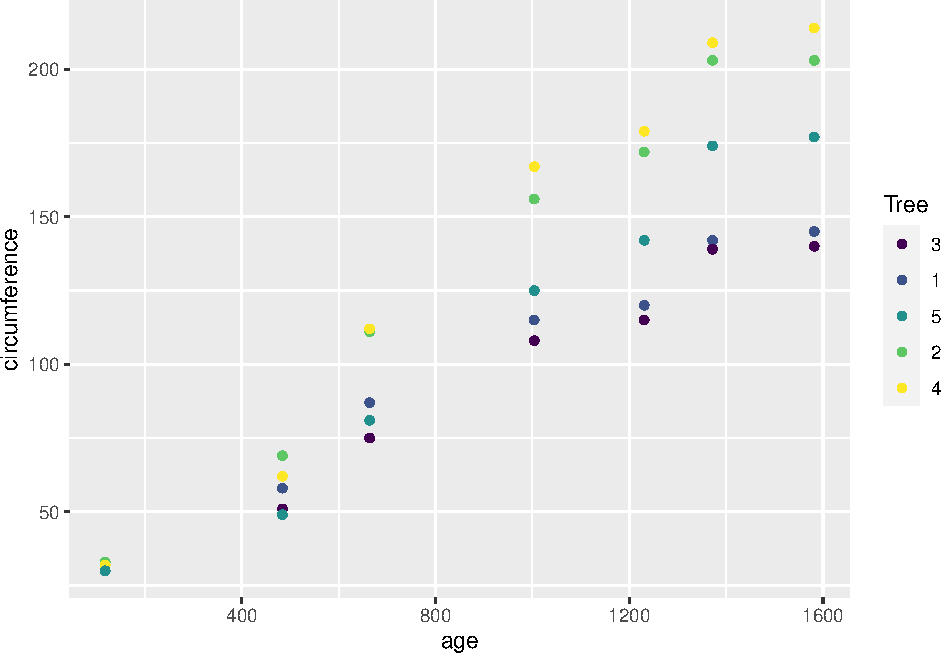
\includegraphics{07-ggplot_files/figure-latex/unnamed-chunk-41-1.pdf}

\begin{enumerate}
\def\labelenumi{\arabic{enumi})}
\setcounter{enumi}{1}
\tightlist
\item
  나무별로 다른 켄버스에 age와 circumference를 x와 y축으로 하는 산점도를 그리는 코드를 작성하시오 (ggplot, facet\_grid이용)
\end{enumerate}

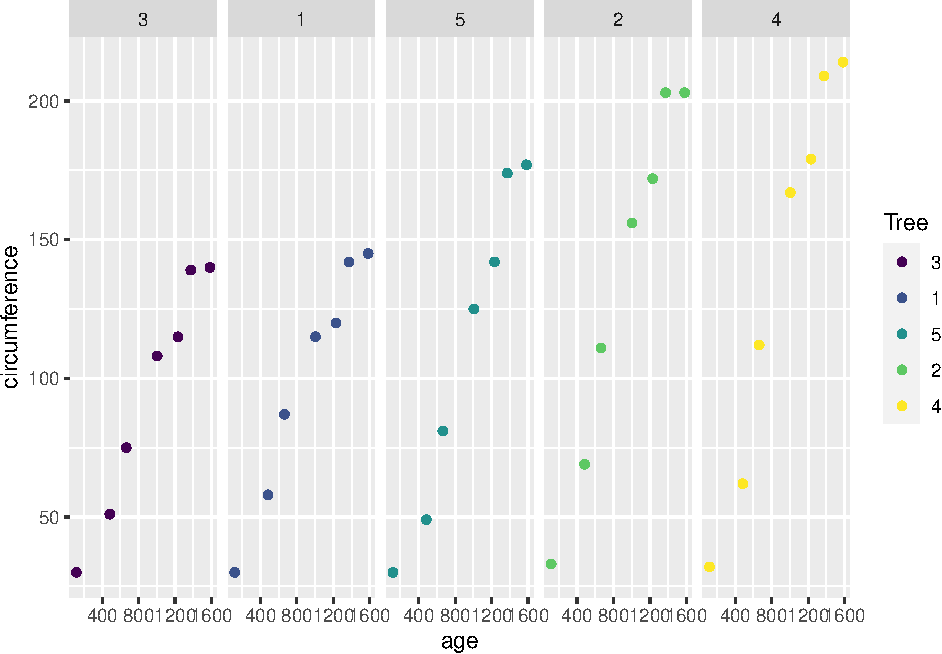
\includegraphics{07-ggplot_files/figure-latex/unnamed-chunk-42-1.pdf}

\begin{enumerate}
\def\labelenumi{\arabic{enumi})}
\setcounter{enumi}{2}
\tightlist
\item
  2)에서 그려진 나무별 산점도에 다음과 같이 선분을 추가한 그래프를 그리는 코드를 작성 하시오
\end{enumerate}

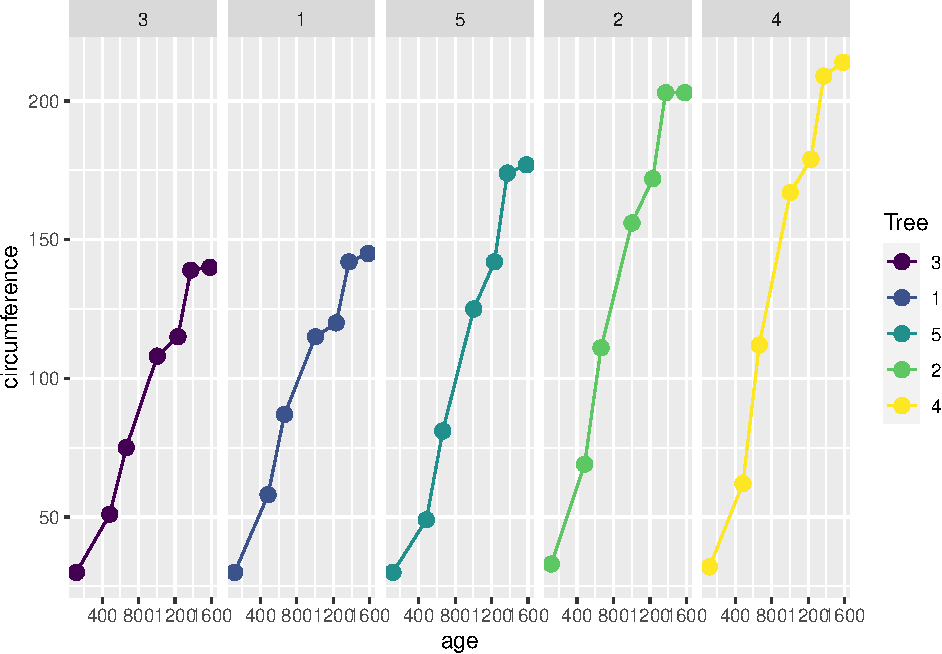
\includegraphics{07-ggplot_files/figure-latex/unnamed-chunk-43-1.pdf}

\textbf{Exercises}

\texttt{InsectSprays}는 제초제의 효능에 관한 데이터이다. 다음과 같은 plot을 그리는 코드를 작성 하시오

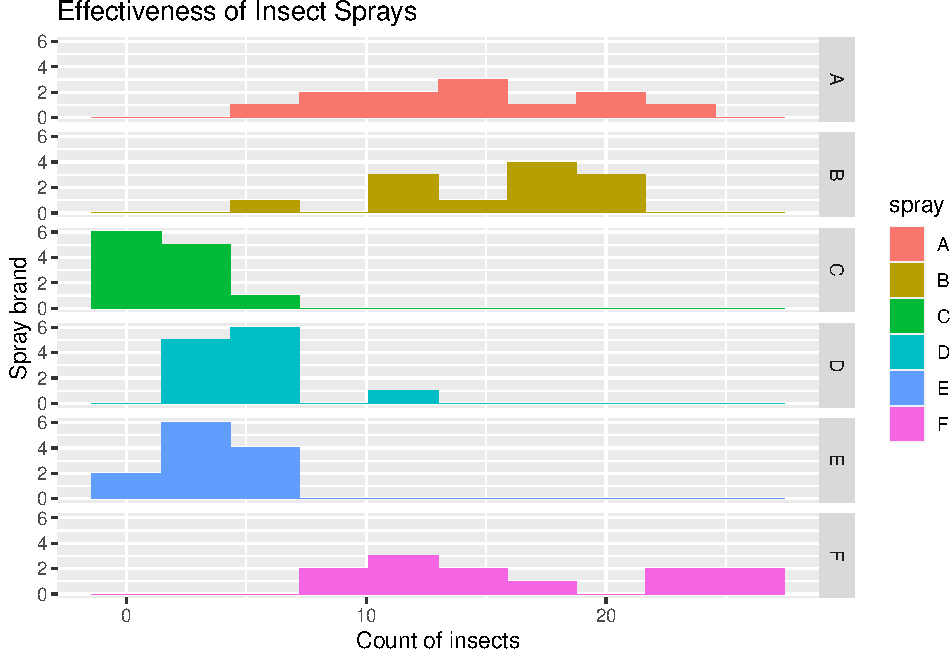
\includegraphics{07-ggplot_files/figure-latex/unnamed-chunk-44-1.pdf}

\hypertarget{themes-labels-and-scales}{%
\section{Themes, Labels, and Scales}\label{themes-labels-and-scales}}

Theme은 data관련 요소들 외의 것들에 대한 설정을 위해서 사용됩니다. 즉, 제목이나 라벨, 배경, 범례 등의 색, 위치, 크기, 모양 등을 설정하는데 사용합니다. 주의할 부분은 해당 택스트 등 데이터를 변경하는 것이 아니고 보여지는 모습만을 바꿀 수 있다는 것 입니다. 택스트 설정은 \texttt{labs}를 사용합니다. 예제를 가지고 몇 가지 실습을 해 보겠습니다. 먼저 \texttt{labs}라는 명령어로 x축, y축, Title 등을 설정할 수 있습니다. 참고로 \texttt{xlab()}, \texttt{ylab()} 등의 함수도 x축, y축 라벨을 설정하는데 사용될 수 있지만 여기서는 \texttt{labs}만을 사용하도록 합니다.

\begin{Shaded}
\begin{Highlighting}[]
\FunctionTok{ggplot}\NormalTok{(mynewdata, }\FunctionTok{aes}\NormalTok{(}\AttributeTok{x=}\NormalTok{classes, }\AttributeTok{fill=}\NormalTok{bloodtype)) }\SpecialCharTok{+}
  \FunctionTok{geom\_bar}\NormalTok{(}\AttributeTok{position=}\StringTok{"dodge"}\NormalTok{) }\SpecialCharTok{+}
  \FunctionTok{labs}\NormalTok{(}\AttributeTok{x=}\StringTok{\textquotesingle{}Four classes\textquotesingle{}}\NormalTok{,}
       \AttributeTok{y=}\StringTok{\textquotesingle{}Number of students\textquotesingle{}}\NormalTok{,}
       \AttributeTok{title=}\StringTok{\textquotesingle{}Blood type distribution\textquotesingle{}}\NormalTok{,}
       \AttributeTok{subtitle =} \StringTok{\textquotesingle{}Blood type distribution from the 200 students\textquotesingle{}}\NormalTok{,}
       \AttributeTok{fill=}\StringTok{\textquotesingle{}Blood Types\textquotesingle{}}\NormalTok{) }
\end{Highlighting}
\end{Shaded}

위 코드에서 \texttt{labs}에서 설정할 수 있는 옵션은 \texttt{title}, \texttt{subtitle}과 x축, y축 라벨 그리고 범례의 title까지 가능합니다. 특히 \texttt{ggplot} 명령에서 \texttt{aes(fill=bloodtype)}이 사용되었으므로 범례의 title은 \texttt{fill="Blood\ types"}로 설정해야 하며 만약 \texttt{aes(color=bloodtype)}으로 사용되었을 경우에는 \texttt{color="Blood\ types"}으로 설정합니다. 참고로 범례의 label을 설정하는 방법은 다음과 같이 \texttt{scale\_fill\_discrete} 함수의 \texttt{labels} 옵션을 사용하면 됩니다. \texttt{element\_blank()}는 택스트를 공백으로 설정할 때 사용합니다. 아래 나올 \texttt{scale} 관련 내용과 함께 이해하시면 좋습니다.

\begin{Shaded}
\begin{Highlighting}[]
\FunctionTok{ggplot}\NormalTok{(mynewdata, }\FunctionTok{aes}\NormalTok{(}\AttributeTok{x=}\NormalTok{classes, }\AttributeTok{fill=}\NormalTok{bloodtype)) }\SpecialCharTok{+}
  \FunctionTok{geom\_bar}\NormalTok{(}\AttributeTok{position=}\StringTok{"dodge"}\NormalTok{) }\SpecialCharTok{+}
  \FunctionTok{scale\_fill\_discrete}\NormalTok{(}\AttributeTok{name=}\FunctionTok{element\_blank}\NormalTok{(), }\AttributeTok{labels=}\FunctionTok{c}\NormalTok{(}\StringTok{"A type"}\NormalTok{, }\StringTok{"AB type"}\NormalTok{, }\StringTok{"B type"}\NormalTok{, }\StringTok{"O type"}\NormalTok{))}
\end{Highlighting}
\end{Shaded}

이제 본격적으로 Theme으로 그래프를 장식해 보도록 합니다. \texttt{Theme} 관련된 옵션들은 \url{https://ggplot2.tidyverse.org/reference/theme.html} 이곳을 참고하시기 바랍니다. 여기서 mapping은 그대로인채로 모양 등의 설정을 바꿔가면서 그래프의 형태를 확인하는 작업이 반복되므로 다음과 같이 \texttt{myplot}이라는 변수에 기본이 되는 ggplot 코드를 저장하고 이후 \texttt{+} 연산자를 사용해서 옵션을 바꿔가며 편리하게 코드를 재사용 할 수도 있습니다.

\begin{Shaded}
\begin{Highlighting}[]
\NormalTok{myplot }\OtherTok{\textless{}{-}} \FunctionTok{ggplot}\NormalTok{(mynewdata, }\FunctionTok{aes}\NormalTok{(}\AttributeTok{x=}\NormalTok{classes, }\AttributeTok{fill=}\NormalTok{bloodtype)) }\SpecialCharTok{+}
  \FunctionTok{geom\_bar}\NormalTok{(}\AttributeTok{position=}\StringTok{"dodge"}\NormalTok{) }\SpecialCharTok{+}
  \FunctionTok{labs}\NormalTok{(}\AttributeTok{x=}\StringTok{\textquotesingle{}Four classes\textquotesingle{}}\NormalTok{,}
       \AttributeTok{y=}\StringTok{\textquotesingle{}Number of students\textquotesingle{}}\NormalTok{,}
       \AttributeTok{title=}\StringTok{\textquotesingle{}Blood type distribution\textquotesingle{}}\NormalTok{,}
       \AttributeTok{subtitle =} \StringTok{\textquotesingle{}Blood type distribution from the 200 students\textquotesingle{}}\NormalTok{,}
       \AttributeTok{fill=}\StringTok{\textquotesingle{}Blood Types\textquotesingle{}}\NormalTok{) }
\NormalTok{myplot }\SpecialCharTok{+} \FunctionTok{theme\_bw}\NormalTok{()}
\end{Highlighting}
\end{Shaded}

위 \texttt{theme\_bw()} 함수는 theme의 세부 사항 몇 가지를 미리 설정해 놓아서 (배경을 white 색, 눈금을 회색으로 바꾸는 등) theme 설정을 위한 일련의 과정을 한번에 수행하도록 만든 함수 입니다. theme을 이용한 설정은 plot, axis, legend, panel, facet 등에 적용할 수 있으며 따라서 다음 코드와 같이 해당하는 요소를 참고할 때 \texttt{.} 기호로 구분된 옵션 이름을 사용합니다. 값을 지정할 때에는 \texttt{element\_xxx}의 패턴으로 이루어진 함수를 사용합니다. 다음은 각각 plot과 panel 배경색을 바꾸는 코드 입니다.

\begin{Shaded}
\begin{Highlighting}[]
\NormalTok{myplot }\SpecialCharTok{+} \FunctionTok{theme}\NormalTok{(}\AttributeTok{plot.background =} \FunctionTok{element\_rect}\NormalTok{(}\AttributeTok{fill=}\StringTok{"gray"}\NormalTok{))}
\end{Highlighting}
\end{Shaded}

\begin{Shaded}
\begin{Highlighting}[]
\NormalTok{myplot }\SpecialCharTok{+} \FunctionTok{theme}\NormalTok{(}\AttributeTok{panel.background =} \FunctionTok{element\_rect}\NormalTok{(}\AttributeTok{fill=}\StringTok{"gray"}\NormalTok{))}
\end{Highlighting}
\end{Shaded}

\begin{Shaded}
\begin{Highlighting}[]
\NormalTok{myplot }\SpecialCharTok{+} 
  \FunctionTok{theme}\NormalTok{(}
    \AttributeTok{panel.background =} \FunctionTok{element\_rect}\NormalTok{(}\AttributeTok{fill=}\StringTok{"gray"}\NormalTok{),}
    \AttributeTok{plot.background =} \FunctionTok{element\_rect}\NormalTok{(}\AttributeTok{fill=}\StringTok{"gray"}\NormalTok{)}
\NormalTok{    )}
\end{Highlighting}
\end{Shaded}

또한 축이나 라벨 택스트의 모양도 바꿀 수 있습니다.

\begin{Shaded}
\begin{Highlighting}[]
\NormalTok{myplot }\SpecialCharTok{+} 
  \FunctionTok{theme}\NormalTok{(}
    \AttributeTok{axis.line =} \FunctionTok{element\_line}\NormalTok{(}\AttributeTok{arrow =} \FunctionTok{arrow}\NormalTok{(}\AttributeTok{angle =} \DecValTok{15}\NormalTok{, }\AttributeTok{length =} \FunctionTok{unit}\NormalTok{(.}\DecValTok{15}\NormalTok{,}\StringTok{"inches"}\NormalTok{))),}
    \AttributeTok{axis.text =} \FunctionTok{element\_text}\NormalTok{(}\AttributeTok{face =} \StringTok{"bold"}\NormalTok{, }\AttributeTok{size =} \DecValTok{12}\NormalTok{, }\AttributeTok{angle =} \DecValTok{30}\NormalTok{),}
    \AttributeTok{axis.text.x =} \FunctionTok{element\_text}\NormalTok{(}\AttributeTok{color=}\StringTok{"blue"}\NormalTok{, }\AttributeTok{size=}\DecValTok{18}\NormalTok{)}
\NormalTok{    )}
\end{Highlighting}
\end{Shaded}

\begin{Shaded}
\begin{Highlighting}[]
\NormalTok{myplot }\SpecialCharTok{+} 
  \FunctionTok{theme}\NormalTok{(}
    \AttributeTok{plot.title=}\FunctionTok{element\_text}\NormalTok{(}\AttributeTok{size=}\DecValTok{18}\NormalTok{, }\AttributeTok{face =} \StringTok{"bold"}\NormalTok{, }\AttributeTok{color=}\StringTok{"red"}\NormalTok{, }\AttributeTok{hjust=}\FloatTok{0.5}\NormalTok{),}
    \AttributeTok{plot.subtitle =} \FunctionTok{element\_text}\NormalTok{(}\AttributeTok{size=}\DecValTok{18}\NormalTok{, }\AttributeTok{face =} \StringTok{"bold"}\NormalTok{, }\AttributeTok{color=}\StringTok{"gray"}\NormalTok{)}
\NormalTok{    )}
\end{Highlighting}
\end{Shaded}

위 예제 외에도 다양한 그래프를 그릴 수 있으며 모든 사용법을 외워서 사용하기 보다는 사용할 때 마다 필요한 함수와 옵션을 찾아서 사용하다 보면 점차 익숙해질 것 입니다. 가장 정확한 참고 자료는 공식 reference 페이지를 참고하면 좋으며 \url{https://ggplot2.tidyverse.org/reference/index.html} 이 외에도 다른 사람들이 만들어 놓은 그래프를 \url{https://exts.ggplot2.tidyverse.org/} 참고해서 원하는 목적에 맞는 코드를 가져다 사용할 수 있습니다.

본 장에서 마지막으로 소개할 내용은 \texttt{Scale} 입니다. 앞서 어떤 데이터를 x축, y축 또는 group이나 color로 맵핑할지를 결정하는 함수가 \texttt{aes}였다면 scale은 어떻게 (위치, 색상, 크기, 모양 등) 맵핑할 것인가를 설정하는 방법입니다. 함수 형태는 \texttt{scale\_\textless{}aesthetic\textgreater{}\_\textless{}type\textgreater{}} 이며 \texttt{\textless{}aesthetic\textgreater{}}과 \texttt{\textless{}type\textgreater{}}에 해당하는 (미리 지정된) 단어를 넣어주면 되겠습니다. 예를 들어 앞서 예제에서 \texttt{fill=bloodtype}로 혈액형 데이터를 막대그래프의 색을 칠하는데 사용했다면 \texttt{scale\_fill\_manual} 함수로 어떤 색을 칠할지를 정해주는 방식입니다. 다음 몇 가지 예를 실습해 보고 이해해 봅니다.

\begin{Shaded}
\begin{Highlighting}[]
\NormalTok{myplot }\SpecialCharTok{+} 
  \FunctionTok{scale\_fill\_manual}\NormalTok{(}\AttributeTok{values =} \FunctionTok{c}\NormalTok{(}\StringTok{"orange"}\NormalTok{, }\StringTok{"skyblue"}\NormalTok{, }\StringTok{"royalblue"}\NormalTok{, }\StringTok{"blue"}\NormalTok{))}

\NormalTok{myplot }\SpecialCharTok{+} 
  \FunctionTok{scale\_fill\_brewer}\NormalTok{(}\AttributeTok{palette=}\StringTok{"BrBG"}\NormalTok{)}
\end{Highlighting}
\end{Shaded}

두 번째 \texttt{scale\_fill\_brewer}의 경우는 \texttt{brewer}라는 (\url{https://colorbrewer2.org/}) 미리 지정된 색의 조합을 가져와 사용하는 방식입니다. \texttt{?scale\_fill\_brewer}의 Palettes 섹션을 보시면 사용 가능한 팔레트의 이름이 나와 있으며 위 예제 에서는 BrBG라는 이름의 팔레트를 사용했습니다. 아래는 viridis 라는 이름의 팔레트이며 (\url{https://bids.github.io/colormap/}) 이러한 팔레트는 R 뿐만 아니라 python, Matlab 등의 다른 프로그래밍 언어에서도 사용할 수 있도록 라이브러리를 제공하고 있습니다.

\begin{Shaded}
\begin{Highlighting}[]
\NormalTok{myplot }\SpecialCharTok{+} 
  \FunctionTok{scale\_fill\_viridis\_d}\NormalTok{()}
\end{Highlighting}
\end{Shaded}

참고로 앞서 설명한 바와 같이 \texttt{aes(fill=bloodtype)}이 사용되었으므로 \texttt{scale\_fill\_viridis\_d}을 사용했으며 만약 \texttt{aes(color=bloodtype)}으로 사용되었을 경우에는 이에 맞는 \texttt{scale\_fill\_viridis\_d}으로 설정해야 합니다. 맵핑된 데이터가 연속형일 경우에는 (위 학급 예제의 혈액형은 4개의 혈액형으로 나뉘는 범주형 데이터임) \texttt{scale\_fill\_gradient}, \texttt{scale\_fill\_distiller} 등의 연속형 데이터에 맞는 scale 함수를 사용해야 합니다. 또한 데이터의 스케일이 log나 지수 단위일 경우에도 일 때에도 \texttt{scale\_x\_log10()} 등의 함수를 이용해서 x축 또는 y축의 스케일을 변경해줄 수 있습니다. 다음은 간단한 형태의 로그 분포 데이터를 생성하고 히스토그램을 그리는 코드입니다.

\begin{Shaded}
\begin{Highlighting}[]
\NormalTok{mydf }\OtherTok{\textless{}{-}} \FunctionTok{data.frame}\NormalTok{(}\AttributeTok{x=}\FunctionTok{rlnorm}\NormalTok{(}\DecValTok{1000}\NormalTok{, }\FunctionTok{log}\NormalTok{(}\DecValTok{10}\NormalTok{), }\FunctionTok{log}\NormalTok{(}\FloatTok{2.5}\NormalTok{)))}
\NormalTok{p }\OtherTok{\textless{}{-}} \FunctionTok{ggplot}\NormalTok{(mydf, }\FunctionTok{aes}\NormalTok{(}\AttributeTok{x=}\NormalTok{x)) }\SpecialCharTok{+}
  \FunctionTok{geom\_histogram}\NormalTok{()}
\NormalTok{p}
\end{Highlighting}
\end{Shaded}

위 히스토그램의 x축을 로그 스케일로 전환하고자 할 때 다음과 같이 \texttt{scale\_x\_log10()} 함수를 추가하면 됩니다.

\begin{Shaded}
\begin{Highlighting}[]
\NormalTok{p }\SpecialCharTok{+} \FunctionTok{scale\_x\_log10}\NormalTok{()}
\end{Highlighting}
\end{Shaded}

\textbf{Exercises}

\texttt{mpg} 데이터셋은 38종 자동차의 연비 데이터임. 이 데이터셋을 이용하여 다음 그래프를 그리시오

\begin{enumerate}
\def\labelenumi{\arabic{enumi})}
\item
  엔진 배기량과 (displ) 도심연비 (cty)를 비교하는 산포도를 그리고 어떤 연관성이 있는지 설명하시오
\item
  위 산포도의 점들은 실제로는 한 개 이상의 데이터가 겹쳐셔 표현된 경우가 많음. ggplot2에서는 이러한 문제를 극복하기 위해서 \texttt{position="jitter"} 라는 옵션을 사용할 수 있음. 이 옵션을 적용한 코드를 작성하시오.
\item
  위 그래프에 배기량과 (displ) 고속도로연비 (hwy) 산포도를 추가하여 다음과 같이 \texttt{scale\_color\_manual()} 함수를 사용해서 ``red''와 ``blue''로 점들을 표현한 그래프를 그리시오.
\end{enumerate}

\begin{Shaded}
\begin{Highlighting}[]

\NormalTok{mydf }\OtherTok{\textless{}{-}} \FunctionTok{data.frame}\NormalTok{(}\AttributeTok{displ=}\NormalTok{mpg}\SpecialCharTok{$}\NormalTok{displ, }\AttributeTok{cty=}\NormalTok{mpg}\SpecialCharTok{$}\NormalTok{cty, }\AttributeTok{hwy=}\NormalTok{mpg}\SpecialCharTok{$}\NormalTok{hwy) }\SpecialCharTok{\%\textgreater{}\%} 
  \FunctionTok{pivot\_longer}\NormalTok{(}\AttributeTok{cols=}\FunctionTok{c}\NormalTok{(}\StringTok{"cty"}\NormalTok{, }\StringTok{"hwy"}\NormalTok{), }\AttributeTok{names\_to=}\StringTok{"type"}\NormalTok{)}
\FunctionTok{str}\NormalTok{(mydf)}
\end{Highlighting}
\end{Shaded}

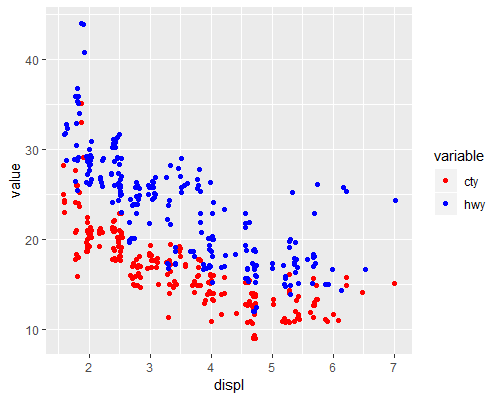
\includegraphics{images/06/ex6-4-2.png}

\begin{enumerate}
\def\labelenumi{\arabic{enumi})}
\setcounter{enumi}{3}
\tightlist
\item
  다음과 같이 배기량과 고속도로/도심 연비의 관계를 나타내는 추세선을 추가하시오 (\texttt{geom\_smooth} 이용)
\end{enumerate}

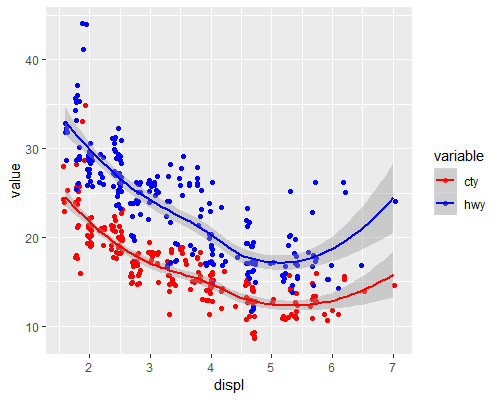
\includegraphics{images/06/ex6-4-4.png}

\begin{enumerate}
\def\labelenumi{\arabic{enumi})}
\setcounter{enumi}{4}
\tightlist
\item
  아래 그림과 같이 Theme을 \texttt{theme\_bw()}를 사용하고 추가로 Title, subtitle, x축, y축 라벨, 그리고 범례의 Title을 변경하시오. (범례의 라벨 설정은 \texttt{scale\_color\_manual}에서 \texttt{labels=c("City\ MPG",\ "Highway\ MPG")}으로 설정, 범례의 title을 지울때는 \texttt{name=element\_blank()}, Title의 택스트 크기는 20, x축, y축의 라벨 텍스트 크기는 18로 설정)
\end{enumerate}

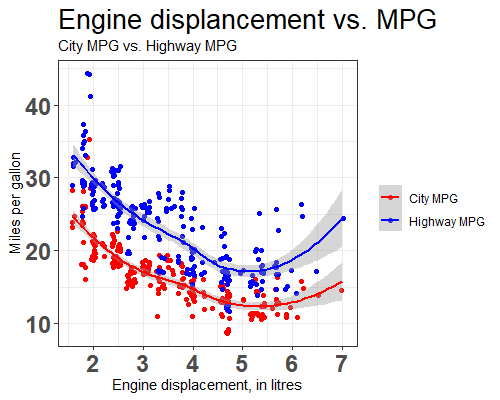
\includegraphics{images/06/ex6-4-5.png}

\hypertarget{ggplot2-examples}{%
\chapter{ggplot2 examples}\label{ggplot2-examples}}

인터넷에서 찾은 다음 사이트의 예제를 보면서 다양한 그래프 예제를 실행해 보겠습니다. 코드는 조금씩 변형된 부분이 있으니 참고 부탁 드립니다.

\begin{itemize}
\tightlist
\item
  \url{https://www.r-graph-gallery.com/ggplot2-package.html}
\item
  \url{http://r-statistics.co/Top50-Ggplot2-Visualizations-MasterList-R-Code.html}
\item
  \url{https://www.datanovia.com/en/blog/ggplot-examples-best-reference/}
\end{itemize}

\hypertarget{violin-plot}{%
\section{Violin plot}\label{violin-plot}}

\begin{itemize}
\tightlist
\item
  \url{https://www.r-graph-gallery.com/violin_and_boxplot_ggplot2.html}
\end{itemize}

\includegraphics{images/10/000013.png}

\begin{Shaded}
\begin{Highlighting}[]
\FunctionTok{library}\NormalTok{(tidyverse)}
\FunctionTok{library}\NormalTok{(viridis)}

\CommentTok{\# create a dataset}
\NormalTok{data }\OtherTok{\textless{}{-}} \FunctionTok{data.frame}\NormalTok{(}
  \AttributeTok{name=}\FunctionTok{c}\NormalTok{( }\FunctionTok{rep}\NormalTok{(}\StringTok{"A"}\NormalTok{,}\DecValTok{500}\NormalTok{), }\FunctionTok{rep}\NormalTok{(}\StringTok{"B"}\NormalTok{,}\DecValTok{500}\NormalTok{), }\FunctionTok{rep}\NormalTok{(}\StringTok{"B"}\NormalTok{,}\DecValTok{500}\NormalTok{), }\FunctionTok{rep}\NormalTok{(}\StringTok{"C"}\NormalTok{,}\DecValTok{20}\NormalTok{), }\FunctionTok{rep}\NormalTok{(}\StringTok{\textquotesingle{}D\textquotesingle{}}\NormalTok{, }\DecValTok{100}\NormalTok{)  ),}
  \AttributeTok{value=}\FunctionTok{c}\NormalTok{( }\FunctionTok{rnorm}\NormalTok{(}\DecValTok{500}\NormalTok{, }\DecValTok{10}\NormalTok{, }\DecValTok{5}\NormalTok{), }\FunctionTok{rnorm}\NormalTok{(}\DecValTok{500}\NormalTok{, }\DecValTok{13}\NormalTok{, }\DecValTok{1}\NormalTok{), }\FunctionTok{rnorm}\NormalTok{(}\DecValTok{500}\NormalTok{, }\DecValTok{18}\NormalTok{, }\DecValTok{1}\NormalTok{), }\FunctionTok{rnorm}\NormalTok{(}\DecValTok{20}\NormalTok{, }\DecValTok{25}\NormalTok{, }\DecValTok{4}\NormalTok{), }\FunctionTok{rnorm}\NormalTok{(}\DecValTok{100}\NormalTok{, }\DecValTok{12}\NormalTok{, }\DecValTok{1}\NormalTok{) )}
\NormalTok{)}

\NormalTok{data }\SpecialCharTok{\%\textgreater{}\%}\NormalTok{ str}

\FunctionTok{ggplot}\NormalTok{(data, }\FunctionTok{aes}\NormalTok{(}\AttributeTok{x=}\NormalTok{name, }\AttributeTok{y=}\NormalTok{value, }\AttributeTok{fill=}\NormalTok{name)) }\SpecialCharTok{+}
    \FunctionTok{geom\_violin}\NormalTok{(}\AttributeTok{width=}\FloatTok{1.4}\NormalTok{) }\SpecialCharTok{+}
    \FunctionTok{geom\_boxplot}\NormalTok{(}\AttributeTok{width=}\FloatTok{0.1}\NormalTok{, }\AttributeTok{alpha=}\FloatTok{0.2}\NormalTok{) }

\CommentTok{\# sample summary}
\NormalTok{sample\_size }\OtherTok{=}\NormalTok{ data }\SpecialCharTok{\%\textgreater{}\%} 
  \FunctionTok{group\_by}\NormalTok{(name) }\SpecialCharTok{\%\textgreater{}\%} 
  \FunctionTok{summarize}\NormalTok{(}\AttributeTok{num=}\FunctionTok{n}\NormalTok{()) }

\NormalTok{xlab }\OtherTok{\textless{}{-}}\NormalTok{ sample\_size }\SpecialCharTok{\%\textgreater{}\%} 
  \FunctionTok{apply}\NormalTok{(}\DecValTok{1}\NormalTok{, }\ControlFlowTok{function}\NormalTok{(x)}\FunctionTok{paste0}\NormalTok{(x, }\AttributeTok{collapse=}\StringTok{"}\SpecialCharTok{\textbackslash{}n}\StringTok{ n="}\NormalTok{))}

\FunctionTok{apply}\NormalTok{(sample\_size, }\DecValTok{1}\NormalTok{, }\ControlFlowTok{function}\NormalTok{(x)}\FunctionTok{paste0}\NormalTok{(x, }\AttributeTok{collapse=}\StringTok{"}\SpecialCharTok{\textbackslash{}n}\StringTok{ n="}\NormalTok{))}

\FunctionTok{ggplot}\NormalTok{(data, }\FunctionTok{aes}\NormalTok{(}\AttributeTok{x=}\NormalTok{name, }\AttributeTok{y=}\NormalTok{value, }\AttributeTok{fill=}\NormalTok{name)) }\SpecialCharTok{+}
    \FunctionTok{geom\_violin}\NormalTok{(}\AttributeTok{width=}\FloatTok{1.4}\NormalTok{) }\SpecialCharTok{+}
    \FunctionTok{geom\_boxplot}\NormalTok{(}\AttributeTok{width=}\FloatTok{0.1}\NormalTok{, }\AttributeTok{alpha=}\FloatTok{0.2}\NormalTok{) }\SpecialCharTok{+}
    \FunctionTok{scale\_fill\_viridis}\NormalTok{(}\AttributeTok{discrete =} \ConstantTok{TRUE}\NormalTok{) }\SpecialCharTok{+}
    \FunctionTok{scale\_x\_discrete}\NormalTok{(}\AttributeTok{labels=}\NormalTok{xlab) }\SpecialCharTok{+}
    \FunctionTok{theme}\NormalTok{(}
      \AttributeTok{legend.position=}\StringTok{"none"}\NormalTok{,}
      \AttributeTok{plot.title =} \FunctionTok{element\_text}\NormalTok{(}\AttributeTok{size=}\DecValTok{11}\NormalTok{)}
\NormalTok{    ) }\SpecialCharTok{+}
    \FunctionTok{ggtitle}\NormalTok{(}\StringTok{"A Violin wrapping a boxplot"}\NormalTok{) }\SpecialCharTok{+}
    \FunctionTok{xlab}\NormalTok{(}\StringTok{""}\NormalTok{)}
\end{Highlighting}
\end{Shaded}

\hypertarget{bubble-plot}{%
\section{Bubble plot}\label{bubble-plot}}

\begin{itemize}
\tightlist
\item
  \url{https://www.r-graph-gallery.com/320-the-basis-of-bubble-plot.html}
\end{itemize}

\includegraphics{images/10/000049.png}

\begin{Shaded}
\begin{Highlighting}[]
\NormalTok{mpg }\SpecialCharTok{\%\textgreater{}\%}\NormalTok{ str}

\CommentTok{\# Most basic bubble plot}
\FunctionTok{ggplot}\NormalTok{(mpg, }\FunctionTok{aes}\NormalTok{(}\AttributeTok{x=}\NormalTok{cty, }\AttributeTok{y=}\NormalTok{displ, }\AttributeTok{size =}\NormalTok{ hwy)) }\SpecialCharTok{+}
  \FunctionTok{geom\_point}\NormalTok{(}\AttributeTok{alpha=}\FloatTok{0.7}\NormalTok{, }\AttributeTok{position=}\StringTok{"jitter"}\NormalTok{) }
\end{Highlighting}
\end{Shaded}

\begin{Shaded}
\begin{Highlighting}[]
\FunctionTok{ggplot}\NormalTok{(mpg, }\FunctionTok{aes}\NormalTok{(}\AttributeTok{x=}\NormalTok{cty, }\AttributeTok{y=}\NormalTok{displ, }\AttributeTok{size =}\NormalTok{ hwy)) }\SpecialCharTok{+}
  \FunctionTok{geom\_point}\NormalTok{(}\AttributeTok{alpha=}\FloatTok{0.3}\NormalTok{, }\AttributeTok{position=}\StringTok{"jitter"}\NormalTok{) }\SpecialCharTok{+}
  \FunctionTok{scale\_size}\NormalTok{(}\AttributeTok{range =} \FunctionTok{c}\NormalTok{(.}\DecValTok{1}\NormalTok{, }\DecValTok{7}\NormalTok{), }\AttributeTok{name=}\StringTok{""}\NormalTok{)}
\end{Highlighting}
\end{Shaded}

\begin{Shaded}
\begin{Highlighting}[]
\FunctionTok{ggplot}\NormalTok{(mpg, }\FunctionTok{aes}\NormalTok{(}\AttributeTok{x=}\NormalTok{cty, }\AttributeTok{y=}\NormalTok{displ, }\AttributeTok{size =}\NormalTok{ hwy, }\AttributeTok{color=}\NormalTok{year)) }\SpecialCharTok{+}
  \FunctionTok{geom\_point}\NormalTok{(}\AttributeTok{alpha=}\FloatTok{0.3}\NormalTok{, }\AttributeTok{position=}\StringTok{"jitter"}\NormalTok{) }\SpecialCharTok{+}
  \FunctionTok{scale\_size}\NormalTok{(}\AttributeTok{range =} \FunctionTok{c}\NormalTok{(.}\DecValTok{1}\NormalTok{, }\DecValTok{7}\NormalTok{), }\AttributeTok{name=}\StringTok{""}\NormalTok{)}
\end{Highlighting}
\end{Shaded}

\begin{Shaded}
\begin{Highlighting}[]
\NormalTok{mpg }\SpecialCharTok{\%\textgreater{}\%} 
  \FunctionTok{mutate}\NormalTok{(}\AttributeTok{yearf =} \FunctionTok{factor}\NormalTok{(year)) }\SpecialCharTok{\%\textgreater{}\%} 
  \FunctionTok{ggplot}\NormalTok{(}\FunctionTok{aes}\NormalTok{(}\AttributeTok{x=}\NormalTok{cty, }\AttributeTok{y=}\NormalTok{displ, }\AttributeTok{size=}\NormalTok{hwy, }\AttributeTok{color=}\NormalTok{yearf)) }\SpecialCharTok{+}
  \FunctionTok{geom\_point}\NormalTok{(}\AttributeTok{alpha=}\FloatTok{0.3}\NormalTok{, }\AttributeTok{position=}\StringTok{"jitter"}\NormalTok{) }\SpecialCharTok{+}
  \FunctionTok{scale\_size}\NormalTok{(}\AttributeTok{range =} \FunctionTok{c}\NormalTok{(.}\DecValTok{1}\NormalTok{, }\DecValTok{7}\NormalTok{), }\AttributeTok{name=}\StringTok{""}\NormalTok{) }
\end{Highlighting}
\end{Shaded}

\begin{Shaded}
\begin{Highlighting}[]
\NormalTok{mpg }\SpecialCharTok{\%\textgreater{}\%} 
  \FunctionTok{mutate}\NormalTok{(}\AttributeTok{yearf =} \FunctionTok{factor}\NormalTok{(year)) }\SpecialCharTok{\%\textgreater{}\%} 
  \FunctionTok{ggplot}\NormalTok{(}\FunctionTok{aes}\NormalTok{(}\AttributeTok{x=}\NormalTok{cty, }\AttributeTok{y=}\NormalTok{displ, }\AttributeTok{size=}\NormalTok{hwy, }\AttributeTok{fill=}\NormalTok{yearf)) }\SpecialCharTok{+}
  \FunctionTok{geom\_point}\NormalTok{(}\AttributeTok{alpha=}\FloatTok{0.5}\NormalTok{, }\AttributeTok{position=}\StringTok{"jitter"}\NormalTok{, }\AttributeTok{shape=}\DecValTok{21}\NormalTok{) }\SpecialCharTok{+}
  \FunctionTok{scale\_size}\NormalTok{(}\AttributeTok{range =} \FunctionTok{c}\NormalTok{(.}\DecValTok{1}\NormalTok{, }\DecValTok{7}\NormalTok{), }\AttributeTok{name=}\StringTok{""}\NormalTok{) }\SpecialCharTok{+} 
  \FunctionTok{scale\_fill\_viridis}\NormalTok{(}\AttributeTok{discrete=}\ConstantTok{TRUE}\NormalTok{, }\AttributeTok{guide=}\ConstantTok{FALSE}\NormalTok{, }\AttributeTok{option=}\StringTok{"D"}\NormalTok{) }\SpecialCharTok{+}
  \FunctionTok{theme\_bw}\NormalTok{() }\SpecialCharTok{+}
  \FunctionTok{ylab}\NormalTok{(}\StringTok{"Engine displacement"}\NormalTok{) }\SpecialCharTok{+}
  \FunctionTok{xlab}\NormalTok{(}\StringTok{"City miles per gallon"}\NormalTok{) }\SpecialCharTok{+}
  \FunctionTok{theme}\NormalTok{(}\AttributeTok{legend.position =} \StringTok{"none"}\NormalTok{)}
\end{Highlighting}
\end{Shaded}

\hypertarget{barplot-with-errorbars}{%
\section{Barplot with errorbars}\label{barplot-with-errorbars}}

\includegraphics{images/10/00000e.png}

\begin{Shaded}
\begin{Highlighting}[]
\NormalTok{ToothGrowth }\SpecialCharTok{\%\textgreater{}\%}\NormalTok{ str}

\NormalTok{df }\OtherTok{\textless{}{-}}\NormalTok{ ToothGrowth }\SpecialCharTok{\%\textgreater{}\%} 
  \FunctionTok{mutate}\NormalTok{(}\AttributeTok{dose =} \FunctionTok{as.factor}\NormalTok{(dose))}
\NormalTok{df }\SpecialCharTok{\%\textgreater{}\%}\NormalTok{ str}

\DocumentationTok{\#\# summary}
\NormalTok{df\_summary }\OtherTok{\textless{}{-}}\NormalTok{ df }\SpecialCharTok{\%\textgreater{}\%}
  \FunctionTok{group\_by}\NormalTok{(dose) }\SpecialCharTok{\%\textgreater{}\%}
  \FunctionTok{summarise}\NormalTok{(}\AttributeTok{sd =} \FunctionTok{sd}\NormalTok{(len, }\AttributeTok{na.rm =} \ConstantTok{TRUE}\NormalTok{), }\AttributeTok{len =} \FunctionTok{mean}\NormalTok{(len))}
\NormalTok{df\_summary}


\FunctionTok{ggplot}\NormalTok{(df\_summary, }\FunctionTok{aes}\NormalTok{(}\AttributeTok{x=}\NormalTok{dose, }\AttributeTok{y=}\NormalTok{len, }\AttributeTok{fill=}\NormalTok{dose)) }\SpecialCharTok{+}
  \FunctionTok{geom\_bar}\NormalTok{(}\AttributeTok{stat =} \StringTok{"identity"}\NormalTok{, }\AttributeTok{color =} \StringTok{"black"}\NormalTok{, }\AttributeTok{width =} \FloatTok{0.5}\NormalTok{) }\SpecialCharTok{+}
  \FunctionTok{geom\_errorbar}\NormalTok{(}\FunctionTok{aes}\NormalTok{(}\AttributeTok{ymin =}\NormalTok{ len, }\AttributeTok{ymax =}\NormalTok{ len}\SpecialCharTok{+}\NormalTok{sd), }\AttributeTok{width =} \FloatTok{0.2}\NormalTok{) }
\end{Highlighting}
\end{Shaded}

\hypertarget{horizontal-barplot}{%
\section{horizontal barplot}\label{horizontal-barplot}}

\includegraphics{images/10/00000b.png}

\begin{Shaded}
\begin{Highlighting}[]

\NormalTok{df }\OtherTok{\textless{}{-}}\NormalTok{ mtcars }\SpecialCharTok{\%\textgreater{}\%}
  \FunctionTok{rownames\_to\_column}\NormalTok{() }\SpecialCharTok{\%\textgreater{}\%}
  \FunctionTok{as\_data\_frame}\NormalTok{() }\SpecialCharTok{\%\textgreater{}\%}
  \FunctionTok{mutate}\NormalTok{(}\AttributeTok{cyl =} \FunctionTok{as.factor}\NormalTok{(cyl)) }\SpecialCharTok{\%\textgreater{}\%}
  \FunctionTok{select}\NormalTok{(rowname, wt, mpg, cyl)}
\NormalTok{df}

\CommentTok{\# change fill color by groups and add text labels}
\FunctionTok{ggplot}\NormalTok{(df, }\FunctionTok{aes}\NormalTok{(}\AttributeTok{x =} \FunctionTok{reorder}\NormalTok{(rowname, mpg), }\AttributeTok{y =}\NormalTok{ mpg)) }\SpecialCharTok{+}
  \FunctionTok{geom\_col}\NormalTok{(}\FunctionTok{aes}\NormalTok{(}\AttributeTok{fill =}\NormalTok{ cyl)) }\SpecialCharTok{+} 
  \FunctionTok{geom\_text}\NormalTok{(}\FunctionTok{aes}\NormalTok{(}\AttributeTok{label =}\NormalTok{ mpg), }\AttributeTok{nudge\_y =} \DecValTok{2}\NormalTok{) }\SpecialCharTok{+} 
  \FunctionTok{coord\_flip}\NormalTok{() }\SpecialCharTok{+}
  \FunctionTok{scale\_fill\_viridis\_d}\NormalTok{()}
\end{Highlighting}
\end{Shaded}

\hypertarget{circular-barplot}{%
\section{Circular barplot}\label{circular-barplot}}

\begin{itemize}
\tightlist
\item
  \url{https://www.r-graph-gallery.com/297-circular-barplot-with-groups.html}
\end{itemize}

\includegraphics{images/10/000002.png}

\begin{Shaded}
\begin{Highlighting}[]
\CommentTok{\# Create dataset}
\NormalTok{n }\OtherTok{\textless{}{-}} \DecValTok{70}
\NormalTok{data }\OtherTok{\textless{}{-}} \FunctionTok{data.frame}\NormalTok{(}
  \AttributeTok{id =} \FunctionTok{seq}\NormalTok{(}\DecValTok{1}\NormalTok{, n),}
  \AttributeTok{individual=}\FunctionTok{paste}\NormalTok{( }\StringTok{"Mister "}\NormalTok{, }\FunctionTok{seq}\NormalTok{(}\DecValTok{1}\NormalTok{,n), }\AttributeTok{sep=}\StringTok{""}\NormalTok{),}
  \AttributeTok{group=}\FunctionTok{c}\NormalTok{( }\FunctionTok{rep}\NormalTok{(}\StringTok{\textquotesingle{}A\textquotesingle{}}\NormalTok{, }\DecValTok{10}\NormalTok{), }\FunctionTok{rep}\NormalTok{(}\StringTok{\textquotesingle{}B\textquotesingle{}}\NormalTok{, }\DecValTok{30}\NormalTok{), }\FunctionTok{rep}\NormalTok{(}\StringTok{\textquotesingle{}C\textquotesingle{}}\NormalTok{, }\DecValTok{14}\NormalTok{), }\FunctionTok{rep}\NormalTok{(}\StringTok{\textquotesingle{}D\textquotesingle{}}\NormalTok{, n}\DecValTok{{-}10{-}30{-}14}\NormalTok{)) ,}
  \AttributeTok{value=}\FunctionTok{sample}\NormalTok{( }\FunctionTok{seq}\NormalTok{(}\DecValTok{10}\NormalTok{,}\DecValTok{100}\NormalTok{), n, }\AttributeTok{replace=}\NormalTok{T)}
\NormalTok{)}
\NormalTok{data }\SpecialCharTok{\%\textgreater{}\%}\NormalTok{ str}

\CommentTok{\# introduce NA}
\NormalTok{empty\_bar\_idx }\OtherTok{\textless{}{-}} \FunctionTok{sample}\NormalTok{(}\DecValTok{1}\SpecialCharTok{:}\NormalTok{n, }\DecValTok{10}\NormalTok{)}
\NormalTok{data[empty\_bar\_idx,}\FunctionTok{c}\NormalTok{(}\DecValTok{2}\SpecialCharTok{:}\DecValTok{4}\NormalTok{)] }\OtherTok{\textless{}{-}} \FunctionTok{c}\NormalTok{(}\ConstantTok{NA}\NormalTok{, }\ConstantTok{NA}\NormalTok{, }\ConstantTok{NA}\NormalTok{)}

\NormalTok{label\_data }\OtherTok{\textless{}{-}}\NormalTok{ data}
\NormalTok{number\_of\_bar }\OtherTok{\textless{}{-}} \FunctionTok{nrow}\NormalTok{(label\_data)}
\NormalTok{angle }\OtherTok{\textless{}{-}} \DecValTok{90} \SpecialCharTok{{-}} \DecValTok{360} \SpecialCharTok{*}\NormalTok{ (label\_data}\SpecialCharTok{$}\NormalTok{id}\FloatTok{{-}0.5}\NormalTok{) }\SpecialCharTok{/}\NormalTok{number\_of\_bar     }\CommentTok{\# I substract 0.5 because the letter must have the angle of the center of the bars. Not extreme right(1) or extreme left (0)}
\NormalTok{label\_data}\SpecialCharTok{$}\NormalTok{hjust }\OtherTok{\textless{}{-}} \FunctionTok{ifelse}\NormalTok{( angle }\SpecialCharTok{\textless{}} \SpecialCharTok{{-}}\DecValTok{90}\NormalTok{, }\DecValTok{1}\NormalTok{, }\DecValTok{0}\NormalTok{)}
\NormalTok{label\_data}\SpecialCharTok{$}\NormalTok{angle }\OtherTok{\textless{}{-}} \FunctionTok{ifelse}\NormalTok{(angle }\SpecialCharTok{\textless{}} \SpecialCharTok{{-}}\DecValTok{90}\NormalTok{, angle}\SpecialCharTok{+}\DecValTok{180}\NormalTok{, angle)}

\NormalTok{data }\SpecialCharTok{\%\textgreater{}\%} 
\FunctionTok{ggplot}\NormalTok{(}\FunctionTok{aes}\NormalTok{(}\AttributeTok{x=}\FunctionTok{as.factor}\NormalTok{(id), }\AttributeTok{y=}\NormalTok{value, }\AttributeTok{fill=}\NormalTok{group)) }\SpecialCharTok{+}
  \FunctionTok{geom\_bar}\NormalTok{(}\AttributeTok{stat=}\StringTok{"identity"}\NormalTok{) }\SpecialCharTok{+}
  \FunctionTok{ylim}\NormalTok{(}\SpecialCharTok{{-}}\DecValTok{100}\NormalTok{,}\DecValTok{120}\NormalTok{) }\SpecialCharTok{+}
  \FunctionTok{theme\_minimal}\NormalTok{() }\SpecialCharTok{+}
  \FunctionTok{theme}\NormalTok{(}
    \AttributeTok{axis.text =} \FunctionTok{element\_blank}\NormalTok{(),}
    \AttributeTok{axis.title =} \FunctionTok{element\_blank}\NormalTok{(),}
    \AttributeTok{panel.grid =} \FunctionTok{element\_blank}\NormalTok{(),}
    \AttributeTok{plot.margin =} \FunctionTok{unit}\NormalTok{(}\FunctionTok{rep}\NormalTok{(}\SpecialCharTok{{-}}\DecValTok{1}\NormalTok{,}\DecValTok{4}\NormalTok{), }\StringTok{"cm"}\NormalTok{) }
\NormalTok{  ) }\SpecialCharTok{+}
  \FunctionTok{coord\_polar}\NormalTok{(}\AttributeTok{start =} \DecValTok{0}\NormalTok{) }\SpecialCharTok{+} 
  \FunctionTok{geom\_text}\NormalTok{(}\AttributeTok{data=}\NormalTok{label\_data, }\FunctionTok{aes}\NormalTok{(}\AttributeTok{x=}\NormalTok{id, }\AttributeTok{y=}\NormalTok{value}\SpecialCharTok{+}\DecValTok{10}\NormalTok{, }\AttributeTok{label=}\NormalTok{individual, }\AttributeTok{hjust=}\NormalTok{hjust), }\AttributeTok{color=}\StringTok{"black"}\NormalTok{, }\AttributeTok{fontface=}\StringTok{"bold"}\NormalTok{, }\AttributeTok{alpha=}\FloatTok{0.6}\NormalTok{, }\AttributeTok{size=}\FloatTok{2.5}\NormalTok{, }\AttributeTok{angle=}\NormalTok{ label\_data}\SpecialCharTok{$}\NormalTok{angle, }\AttributeTok{inherit.aes =} \ConstantTok{FALSE}\NormalTok{ ) }
\end{Highlighting}
\end{Shaded}

데이터 정렬 후 plot

\includegraphics{images/10/000008.png}

\begin{Shaded}
\begin{Highlighting}[]

\NormalTok{data2 }\OtherTok{\textless{}{-}}\NormalTok{ data }\SpecialCharTok{\%\textgreater{}\%} 
  \FunctionTok{arrange}\NormalTok{(group, value) }\SpecialCharTok{\%\textgreater{}\%} 
  \FunctionTok{mutate}\NormalTok{(}\AttributeTok{id2=}\DecValTok{1}\SpecialCharTok{:}\FunctionTok{n}\NormalTok{()) }

\NormalTok{label\_data2 }\OtherTok{\textless{}{-}}\NormalTok{ data2}
\NormalTok{number\_of\_bar }\OtherTok{\textless{}{-}} \FunctionTok{nrow}\NormalTok{(label\_data2)}
\NormalTok{angle }\OtherTok{\textless{}{-}} \DecValTok{90} \SpecialCharTok{{-}} \DecValTok{360} \SpecialCharTok{*}\NormalTok{ (label\_data2}\SpecialCharTok{$}\NormalTok{id2}\FloatTok{{-}0.5}\NormalTok{) }\SpecialCharTok{/}\NormalTok{number\_of\_bar     }\CommentTok{\# I substract 0.5 because the letter must have the angle of the center of the bars. Not extreme right(1) or extreme left (0)}
\NormalTok{label\_data2}\SpecialCharTok{$}\NormalTok{hjust }\OtherTok{\textless{}{-}} \FunctionTok{ifelse}\NormalTok{( angle }\SpecialCharTok{\textless{}} \SpecialCharTok{{-}}\DecValTok{90}\NormalTok{, }\DecValTok{1}\NormalTok{, }\DecValTok{0}\NormalTok{)}
\NormalTok{label\_data2}\SpecialCharTok{$}\NormalTok{angle }\OtherTok{\textless{}{-}} \FunctionTok{ifelse}\NormalTok{(angle }\SpecialCharTok{\textless{}} \SpecialCharTok{{-}}\DecValTok{90}\NormalTok{, angle}\SpecialCharTok{+}\DecValTok{180}\NormalTok{, angle)}


\NormalTok{data2 }\SpecialCharTok{\%\textgreater{}\%} 
  \FunctionTok{ggplot}\NormalTok{(}\FunctionTok{aes}\NormalTok{(}\AttributeTok{x=}\FunctionTok{as.factor}\NormalTok{(id2), }\AttributeTok{y=}\NormalTok{value, }\AttributeTok{fill=}\NormalTok{group)) }\SpecialCharTok{+}
  \FunctionTok{geom\_bar}\NormalTok{(}\AttributeTok{stat=}\StringTok{"identity"}\NormalTok{) }\SpecialCharTok{+}
  \FunctionTok{ylim}\NormalTok{(}\SpecialCharTok{{-}}\DecValTok{100}\NormalTok{,}\DecValTok{120}\NormalTok{) }\SpecialCharTok{+}
  \FunctionTok{theme\_minimal}\NormalTok{() }\SpecialCharTok{+}
  \FunctionTok{theme}\NormalTok{(}
    \AttributeTok{axis.text =} \FunctionTok{element\_blank}\NormalTok{(),}
    \AttributeTok{axis.title =} \FunctionTok{element\_blank}\NormalTok{(),}
    \AttributeTok{panel.grid =} \FunctionTok{element\_blank}\NormalTok{(),}
    \AttributeTok{plot.margin =} \FunctionTok{unit}\NormalTok{(}\FunctionTok{rep}\NormalTok{(}\SpecialCharTok{{-}}\DecValTok{1}\NormalTok{,}\DecValTok{4}\NormalTok{), }\StringTok{"cm"}\NormalTok{) }
\NormalTok{  ) }\SpecialCharTok{+}
  \FunctionTok{coord\_polar}\NormalTok{(}\AttributeTok{start =} \DecValTok{0}\NormalTok{) }\SpecialCharTok{+} 
  \FunctionTok{geom\_text}\NormalTok{(}\AttributeTok{data=}\NormalTok{label\_data2, }\FunctionTok{aes}\NormalTok{(}\AttributeTok{x=}\NormalTok{id2, }\AttributeTok{y=}\NormalTok{value}\SpecialCharTok{+}\DecValTok{10}\NormalTok{, }\AttributeTok{label=}\NormalTok{individual, }\AttributeTok{hjust=}\NormalTok{hjust), }\AttributeTok{color=}\StringTok{"black"}\NormalTok{, }\AttributeTok{fontface=}\StringTok{"bold"}\NormalTok{,}\AttributeTok{alpha=}\FloatTok{0.6}\NormalTok{, }\AttributeTok{size=}\FloatTok{2.5}\NormalTok{, }\AttributeTok{angle=}\NormalTok{ label\_data}\SpecialCharTok{$}\NormalTok{angle, }\AttributeTok{inherit.aes =} \ConstantTok{FALSE}\NormalTok{ ) }
\end{Highlighting}
\end{Shaded}

\hypertarget{stacked-area-chart}{%
\section{Stacked area chart}\label{stacked-area-chart}}

\begin{itemize}
\tightlist
\item
  \url{https://www.data-to-viz.com/caveat/stacking.html}
\end{itemize}

\includegraphics{images/10/000009a.png}

\begin{Shaded}
\begin{Highlighting}[]
\FunctionTok{library}\NormalTok{(babynames)}

\NormalTok{babynames }\SpecialCharTok{\%\textgreater{}\%}\NormalTok{ str}


\CommentTok{\# Load dataset from github}
\NormalTok{data }\OtherTok{\textless{}{-}}\NormalTok{ babynames }\SpecialCharTok{\%\textgreater{}\%} 
  \FunctionTok{filter}\NormalTok{(name }\SpecialCharTok{\%in\%} \FunctionTok{c}\NormalTok{(}\StringTok{"Amanda"}\NormalTok{, }\StringTok{"Jessica"}\NormalTok{,    }\StringTok{"Patricia"}\NormalTok{, }\StringTok{"Deborah"}\NormalTok{,   }\StringTok{"Dorothy"}\NormalTok{,  }\StringTok{"Helen"}\NormalTok{)) }\SpecialCharTok{\%\textgreater{}\%}
  \FunctionTok{filter}\NormalTok{(sex}\SpecialCharTok{==}\StringTok{"F"}\NormalTok{)}

\CommentTok{\# Plot}
\NormalTok{p }\OtherTok{\textless{}{-}}\NormalTok{ data }\SpecialCharTok{\%\textgreater{}\%} 
  \FunctionTok{ggplot}\NormalTok{(}\FunctionTok{aes}\NormalTok{(}\AttributeTok{x=}\NormalTok{year, }\AttributeTok{y=}\NormalTok{n, }\AttributeTok{fill=}\NormalTok{name, }\AttributeTok{text=}\NormalTok{name)) }\SpecialCharTok{+}
    \FunctionTok{geom\_area}\NormalTok{( ) }\SpecialCharTok{+}
    \FunctionTok{scale\_fill\_viridis}\NormalTok{(}\AttributeTok{discrete =} \ConstantTok{TRUE}\NormalTok{) }\SpecialCharTok{+}
    \FunctionTok{ggtitle}\NormalTok{(}\StringTok{"Popularity of American names in the previous 30 years"}\NormalTok{) }\SpecialCharTok{+}
    \FunctionTok{theme}\NormalTok{() }\SpecialCharTok{+}
    \FunctionTok{xlab}\NormalTok{(}\StringTok{"Birth year"}\NormalTok{) }\SpecialCharTok{+}
    \FunctionTok{ylab}\NormalTok{(}\StringTok{"Number of babies"}\NormalTok{)}
\NormalTok{p}
\end{Highlighting}
\end{Shaded}

\includegraphics{images/10/000006.png}

\begin{Shaded}
\begin{Highlighting}[]
\NormalTok{p }\SpecialCharTok{+} \FunctionTok{facet\_wrap}\NormalTok{(}\SpecialCharTok{\textasciitilde{}}\NormalTok{name, }\AttributeTok{scale=}\StringTok{"free\_y"}\NormalTok{)}
\end{Highlighting}
\end{Shaded}

\hypertarget{density-plot}{%
\section{Density plot}\label{density-plot}}

\includegraphics{images/10/000003.png}

\begin{Shaded}
\begin{Highlighting}[]
\CommentTok{\# Plot}
\NormalTok{g }\OtherTok{\textless{}{-}} \FunctionTok{ggplot}\NormalTok{(mpg, }\FunctionTok{aes}\NormalTok{(cty))}
\NormalTok{g }\SpecialCharTok{+} \FunctionTok{geom\_density}\NormalTok{(}\FunctionTok{aes}\NormalTok{(}\AttributeTok{fill=}\FunctionTok{factor}\NormalTok{(cyl)), }\AttributeTok{alpha=}\FloatTok{0.8}\NormalTok{) }\SpecialCharTok{+} 
    \FunctionTok{labs}\NormalTok{(}\AttributeTok{title=}\StringTok{"Density plot"}\NormalTok{, }
         \AttributeTok{subtitle=}\StringTok{"City Mileage Grouped by Number of cylinders"}\NormalTok{,}
         \AttributeTok{caption=}\StringTok{"Source: mpg"}\NormalTok{,}
         \AttributeTok{x=}\StringTok{"City Mileage"}\NormalTok{,}
         \AttributeTok{fill=}\StringTok{"\# Cylinders"}\NormalTok{)}
\end{Highlighting}
\end{Shaded}

\hypertarget{waffle-chart}{%
\section{Waffle chart}\label{waffle-chart}}

\begin{itemize}
\tightlist
\item
  \url{http://r-statistics.co/Top50-Ggplot2-Visualizations-MasterList-R-Code.html\#Waffle\%20Chart}
\end{itemize}

\begin{Shaded}
\begin{Highlighting}[]
\NormalTok{var }\OtherTok{\textless{}{-}}\NormalTok{ mpg}\SpecialCharTok{$}\NormalTok{class  }\CommentTok{\# the categorical data }

\DocumentationTok{\#\# Prep data (nothing to change here)}
\NormalTok{nrows }\OtherTok{\textless{}{-}} \DecValTok{10}
\NormalTok{df }\OtherTok{\textless{}{-}} \FunctionTok{expand.grid}\NormalTok{(}\AttributeTok{y =} \DecValTok{1}\SpecialCharTok{:}\NormalTok{nrows, }\AttributeTok{x =} \DecValTok{1}\SpecialCharTok{:}\NormalTok{nrows)}
\NormalTok{categ\_table }\OtherTok{\textless{}{-}} \FunctionTok{round}\NormalTok{(}\FunctionTok{table}\NormalTok{(var) }\SpecialCharTok{*}\NormalTok{ ((nrows}\SpecialCharTok{*}\NormalTok{nrows)}\SpecialCharTok{/}\NormalTok{(}\FunctionTok{length}\NormalTok{(var))))}
\NormalTok{categ\_table}


\NormalTok{df}\SpecialCharTok{$}\NormalTok{category }\OtherTok{\textless{}{-}} \FunctionTok{factor}\NormalTok{(}\FunctionTok{rep}\NormalTok{(}\FunctionTok{names}\NormalTok{(categ\_table), categ\_table))  }
\CommentTok{\# }\AlertTok{NOTE}\CommentTok{: if sum(categ\_table) is not 100 (i.e. nrows\^{}2), it will need adjustment to make the sum to 100.}

\DocumentationTok{\#\# Plot}
\NormalTok{df }\SpecialCharTok{\%\textgreater{}\%}\NormalTok{ str}
\FunctionTok{ggplot}\NormalTok{(df, }\FunctionTok{aes}\NormalTok{(}\AttributeTok{x =}\NormalTok{ x, }\AttributeTok{y =}\NormalTok{ y, }\AttributeTok{fill =}\NormalTok{ category)) }\SpecialCharTok{+} 
        \FunctionTok{geom\_tile}\NormalTok{(}\AttributeTok{color =} \StringTok{"black"}\NormalTok{, }\AttributeTok{size =} \FloatTok{0.5}\NormalTok{) }
\end{Highlighting}
\end{Shaded}

\includegraphics{images/10/00000a.png}

\begin{Shaded}
\begin{Highlighting}[]
\FunctionTok{ggplot}\NormalTok{(df, }\FunctionTok{aes}\NormalTok{(}\AttributeTok{x =}\NormalTok{ x, }\AttributeTok{y =}\NormalTok{ y, }\AttributeTok{fill =}\NormalTok{ category)) }\SpecialCharTok{+} 
        \FunctionTok{geom\_tile}\NormalTok{(}\AttributeTok{color =} \StringTok{"black"}\NormalTok{, }\AttributeTok{size =} \FloatTok{0.5}\NormalTok{) }\SpecialCharTok{+}
        \FunctionTok{scale\_x\_continuous}\NormalTok{(}\AttributeTok{expand =} \FunctionTok{c}\NormalTok{(}\DecValTok{0}\NormalTok{, }\DecValTok{0}\NormalTok{)) }\SpecialCharTok{+}
        \FunctionTok{scale\_y\_continuous}\NormalTok{(}\AttributeTok{expand =} \FunctionTok{c}\NormalTok{(}\DecValTok{0}\NormalTok{, }\DecValTok{0}\NormalTok{), }\AttributeTok{trans =} \StringTok{\textquotesingle{}reverse\textquotesingle{}}\NormalTok{) }\SpecialCharTok{+}
        \FunctionTok{scale\_fill\_brewer}\NormalTok{(}\AttributeTok{palette =} \StringTok{"Set3"}\NormalTok{) }\SpecialCharTok{+}
        \FunctionTok{labs}\NormalTok{(}\AttributeTok{title=}\StringTok{"Waffle Chart"}\NormalTok{, }\AttributeTok{subtitle=}\StringTok{"\textquotesingle{}Class\textquotesingle{} of vehicles"}\NormalTok{,}
             \AttributeTok{caption=}\StringTok{"Source: mpg"}\NormalTok{) }\SpecialCharTok{+} 
        \FunctionTok{theme}\NormalTok{(}\AttributeTok{plot.title =} \FunctionTok{element\_text}\NormalTok{(}\AttributeTok{size =} \FunctionTok{rel}\NormalTok{(}\FloatTok{1.2}\NormalTok{)),}
              \AttributeTok{axis.text =} \FunctionTok{element\_blank}\NormalTok{(),}
              \AttributeTok{axis.title =} \FunctionTok{element\_blank}\NormalTok{(),}
              \AttributeTok{axis.ticks =} \FunctionTok{element\_blank}\NormalTok{(),}
              \AttributeTok{legend.title =} \FunctionTok{element\_blank}\NormalTok{(),}
              \AttributeTok{legend.position =} \StringTok{"right"}\NormalTok{)}
\end{Highlighting}
\end{Shaded}

\hypertarget{marginal-histogram}{%
\section{Marginal histogram}\label{marginal-histogram}}

\includegraphics{images/10/000046.png}

\begin{Shaded}
\begin{Highlighting}[]
\FunctionTok{library}\NormalTok{(ggExtra)}

\CommentTok{\# Scatterplot}
\NormalTok{p }\OtherTok{\textless{}{-}} \FunctionTok{ggplot}\NormalTok{(mpg, }\FunctionTok{aes}\NormalTok{(}\AttributeTok{x=}\NormalTok{cty, }\AttributeTok{y=}\NormalTok{hwy)) }\SpecialCharTok{+} 
  \FunctionTok{geom\_point}\NormalTok{(}\AttributeTok{position=}\StringTok{"jitter"}\NormalTok{, }\AttributeTok{alpha=}\FloatTok{0.5}\NormalTok{) }\SpecialCharTok{+}
  \FunctionTok{geom\_smooth}\NormalTok{(}\AttributeTok{method=}\StringTok{"lm"}\NormalTok{, }\AttributeTok{se=}\NormalTok{F) }\SpecialCharTok{+}
  \FunctionTok{theme\_bw}\NormalTok{() }\SpecialCharTok{+}
  \FunctionTok{theme}\NormalTok{(}
    \AttributeTok{legend.position =} \StringTok{"none"}
\NormalTok{  ) }\SpecialCharTok{+}
  \FunctionTok{xlab}\NormalTok{(}\StringTok{"City miles per gallon"}\NormalTok{) }\SpecialCharTok{+}
  \FunctionTok{ylab}\NormalTok{(}\StringTok{"Highway miles per gallon"}\NormalTok{)}
\NormalTok{p}
\FunctionTok{ggMarginal}\NormalTok{(p, }\AttributeTok{type =} \StringTok{"histogram"}\NormalTok{, }\AttributeTok{fill=}\StringTok{"transparent"}\NormalTok{) }
\FunctionTok{ggMarginal}\NormalTok{(p, }\AttributeTok{type =} \StringTok{"density"}\NormalTok{, }\AttributeTok{fill=}\StringTok{"transparent"}\NormalTok{)}
\end{Highlighting}
\end{Shaded}

\includegraphics{images/10/000005.png}

\begin{Shaded}
\begin{Highlighting}[]
\FunctionTok{library}\NormalTok{(ggpubr)}
\CommentTok{\# Grouped Scatter plot with marginal density plots}
\FunctionTok{ggscatterhist}\NormalTok{(}
\NormalTok{  iris, }
  \AttributeTok{x =} \StringTok{"Sepal.Length"}\NormalTok{, }
  \AttributeTok{y =} \StringTok{"Sepal.Width"}\NormalTok{,}
  \AttributeTok{color =} \StringTok{"Species"}\NormalTok{, }
  \AttributeTok{size =} \DecValTok{3}\NormalTok{, }
  \AttributeTok{alpha =} \FloatTok{0.6}\NormalTok{,}
  \AttributeTok{palette =} \FunctionTok{c}\NormalTok{(}\StringTok{"\#00AFBB"}\NormalTok{, }\StringTok{"\#E7B800"}\NormalTok{, }\StringTok{"\#FC4E07"}\NormalTok{),}
  \AttributeTok{margin.params =} \FunctionTok{list}\NormalTok{(}\AttributeTok{fill =} \StringTok{"Species"}\NormalTok{, }\AttributeTok{color =} \StringTok{"black"}\NormalTok{, }\AttributeTok{size =} \FloatTok{0.2}\NormalTok{)}
\NormalTok{  )}
\end{Highlighting}
\end{Shaded}

\hypertarget{density-ridgeline-plots}{%
\section{Density ridgeline plots}\label{density-ridgeline-plots}}

\includegraphics{images/10/000004.png}

\begin{Shaded}
\begin{Highlighting}[]
\FunctionTok{library}\NormalTok{(ggridges)}
\FunctionTok{ggplot}\NormalTok{(iris, }\FunctionTok{aes}\NormalTok{(}\AttributeTok{x =}\NormalTok{ Sepal.Length, }\AttributeTok{y =}\NormalTok{ Species)) }\SpecialCharTok{+}
  \FunctionTok{geom\_density\_ridges}\NormalTok{(}\FunctionTok{aes}\NormalTok{(}\AttributeTok{fill =}\NormalTok{ Species)) }\SpecialCharTok{+}
  \FunctionTok{scale\_fill\_manual}\NormalTok{(}\AttributeTok{values =} \FunctionTok{c}\NormalTok{(}\StringTok{"\#00AFBB"}\NormalTok{, }\StringTok{"\#E7B800"}\NormalTok{, }\StringTok{"\#FC4E07"}\NormalTok{))}
\end{Highlighting}
\end{Shaded}

\begin{center}\rule{0.5\linewidth}{0.5pt}\end{center}

이 저작물은 크리에이티브 커먼즈 저작자표시-비영리-변경금지 4.0 국제 라이선스에 따라 이용할 수 있습니다.

\hypertarget{bioconductor}{%
\chapter{Bioconductor}\label{bioconductor}}

\begin{itemize}
\tightlist
\item
  \url{https://www.bioconductor.org}
\end{itemize}

Bioconductor는 바이오인포메틱스를 위한 R기반의 데이터, 메소드, 그리고 패키지들의 모음입니다. 2002년 microarray 데이터 분석을 위한 플랫폼으로 시작되었으며 현재 2000개 이상의 패키지로 구성되어 있습니다. R은 분산형 오픈소스이나 Bioconductor는 Full-time developer들에 의해서 유지되고 있습니다. \texttt{CRAN}에 배포되지 않고 \texttt{CRAN}에 비해 더 많은 필수 자료들 (vignettes 등)이 필요하며 높은 수준으로 quality control이 되고 있습니다. Bioconductor는 6개월마다 예정된 릴리스를 통해 모든 bioconductor 패키지가 충돌없이 조화롭게 작동하도록 유지되고 있습니다.

사용 가능한 패키지들은 \href{http://bioconductor.org/packages/release/BiocViews.html\#___Software}{이곳}을 참고하시면 되겠습니다.

\includegraphics[width=6.25in,height=\textheight]{images/04/bioconductor.JPG}

Bioconductor 코어 개발 그룹은 사용자들이 지놈스케일 데이터를 더 편리하게 다루룰 수 있도록 데이터의 구조를 개발하고 있습니다. Bioconductor의 주요 기능은 다음과 같습니다.

\begin{itemize}
\tightlist
\item
  지놈스케일의 서열이나 발현등 대용량 유전자형 데이터 \textbf{관리} 및 \textbf{통계적 분석}을 위한 툴 제공
\item
  분자수준의 현상과 생장이나 질병 등 표현형수준의 관계를 규명하기 위한 정량 데이터 통합 및 관리
\end{itemize}

\hypertarget{packages}{%
\section{Packages}\label{packages}}

메인화면 \textgreater\textgreater{} Use \textgreater\textgreater{} Software, Annotation, Experiment

\begin{itemize}
\tightlist
\item
  Software: 데이터 분석을 위한 알고리즘/툴 모음
\item
  Annotation: 유전자 symbol/ID mapping, gene ontology 기반 유전자 분류, 유전체상에서 exon, transcript, gene 등의 위치, 단백질 기능 등. Annotation \textgreater{} Packagetype 참고
\item
  Experiment data: 검증된 실험 데이터
\item
  Workflow: 특정 데이터 분석을 위한 프로세스 모음 RNA-seq, ChIP seq, copy number analysis, microarray methylation, classic expression analysis, flow cytometry 등
\end{itemize}

\includegraphics[width=6.25in,height=\textheight]{images/bioconductor_list.PNG}

Annotation 리소스는 다음과 같이 몇 단계의 레벨로 구분할 수 있습니다.

\begin{itemize}
\tightlist
\item
  ChipDb: 가장 낮은 단계, Affymatrix Chip 정보
\item
  OrgDb: 특정 생물(Organism)의 기능적 annotations
\item
  TxDb/EnsDb: 전사체 정보, 위치 정보
\item
  OrganismDb: meta-packages for OrgDb, TxDb
\item
  BSgenome 특정 생물의 실제 염기 정보
\item
  Others GO.db; KEGG.db
\item
  AnnotationHub:
\item
  biomaRt:
\end{itemize}

\texttt{Bioconductor}에서 제공하는 패키지를 설치하기 위해서는 \texttt{BiocManager}를 먼저 설치하고 해당 패키지를 설치하시기 바랍니다. \texttt{BiocManager}에는 \texttt{available()}이라는 함수로 (특정 문자가 포함된) 사용 가능한 패키지를 검색할 수 도 있습니다. 예를 들어 \texttt{IRanges}라는 패키지를 설치할 경우 bioconductor 상단 오른쪽의 \texttt{Search} 나 \href{https://www.bioconductor.org/packages/release/BiocViews.html\#___Software}{software package list}의 검색창에서 \texttt{IRanges}를 입력하여 해당 패키지를 찾고 다음과 같이 설치를 수행합니다.

\begin{Shaded}
\begin{Highlighting}[]
\ControlFlowTok{if}\NormalTok{ (}\SpecialCharTok{!}\FunctionTok{requireNamespace}\NormalTok{(}\StringTok{"BiocManager"}\NormalTok{, }\AttributeTok{quietly =} \ConstantTok{TRUE}\NormalTok{))}
    \FunctionTok{install.packages}\NormalTok{(}\StringTok{"BiocManager"}\NormalTok{)}

\NormalTok{BiocManager}\SpecialCharTok{::}\FunctionTok{install}\NormalTok{(}\StringTok{"IRanges"}\NormalTok{)}
\DocumentationTok{\#\# .libPaths()}
\end{Highlighting}
\end{Shaded}

\textbf{Exercises }

OrganismDb는 meta-package의 형태로 OrgDb, TxDb, 그리고 GO.db 패키지들을 포함하는 정보를 가지고 있음. OrganismDB 중 인간의 정보를 가진 \texttt{Homo.sapiens}를 찾아 설치하시오

\hypertarget{learning-and-support}{%
\section{Learning and support}\label{learning-and-support}}

각 패키지는 제목, 저자, 유지관리자, 설명, 참조, 설치법 등의 정보가 포함된 landing page가 있으며 패키지 내 함수들은 상세한 설명과 예제가 제공됩니다. 예를 들어 \href{http://bioconductor.org/packages/release/bioc/html/IRanges.html}{IRanges}의 landing page를 참고하세요. \texttt{vignettes}는 bioconductor의 중요한 특징 중 하나로 R 코드와 함께 패키지를 사용하는 방법에 대한 상세한 설명을 제공하는 문서입니다.

\begin{Shaded}
\begin{Highlighting}[]

\FunctionTok{library}\NormalTok{(IRanges)}

\FunctionTok{vignette}\NormalTok{(}\AttributeTok{package=}\StringTok{"IRanges"}\NormalTok{)}
\FunctionTok{browseVignettes}\NormalTok{(}\StringTok{"IRanges"}\NormalTok{)}
\FunctionTok{vignette}\NormalTok{(}\StringTok{"IRangesOverview"}\NormalTok{, }\AttributeTok{package=}\StringTok{"IRanges"}\NormalTok{)}

\NormalTok{ir1 }\OtherTok{\textless{}{-}} \FunctionTok{IRanges}\NormalTok{(}\AttributeTok{start=}\DecValTok{1}\SpecialCharTok{:}\DecValTok{10}\NormalTok{, }\AttributeTok{width=}\DecValTok{10}\SpecialCharTok{:}\DecValTok{1}\NormalTok{)}
\NormalTok{ir1}
\FunctionTok{class}\NormalTok{(ir1)}
\FunctionTok{methods}\NormalTok{(}\AttributeTok{class=}\StringTok{"IRanges"}\NormalTok{)}

\FunctionTok{example}\NormalTok{(IRanges)}
\NormalTok{?IRanges}
\NormalTok{??IRanges}
\end{Highlighting}
\end{Shaded}

메인페이지 \textgreater\textgreater{} Learn \textgreater\textgreater{} Support site 게시판에는 관련된 여러 QnA 들이 있어서 유사 문제에 대한 도움을 받을 수 있습니다.

\hypertarget{oop---class-object-and-method}{%
\section{OOP - Class, Object and Method}\label{oop---class-object-and-method}}

객체지향프로그래밍 (OOP)은 복잡한 문제를 프로그래밍할 때 발생되는 코드의 복잡성을 해결할 수 있는 하나의 방안으로 1990년대부터 많이 사용되었습니다.

R도 객체지향 프로그래밍 언어입니다. 그런데 R은 다른 언어들에 비해서 좀 어려운 (다른) 개념으로 사용됩니다. R에서 사용하는 Class에는 크게 base type, S3, S4, RC, 그리고 R6 등 다양한 타입이 있고 이 중 S3를 많이 사용해 왔으며 S3의 단점을 보완한 S4 형식의 class와 R6를 주로 사용합니다 \citep{AdvancedR}. 본 강의에서는 S3 형식의 class만 다루도록 하겠습니다.

클래스를 사용하는 이유는 여러가지가 있겠지만 복잡한 개념의 데이터를 구조화하고 쉽게 관리하기 위해서 사용한다고 보면 될 것 같습니다. 여러분이 알아야할 개념은 Class와 Object 그리고 Method 입니다. 사실 R의 모든것이 Object이고 이러한 Object들의 정의가 Class 입니다.

\begin{Shaded}
\begin{Highlighting}[]

\NormalTok{df }\OtherTok{\textless{}{-}} \FunctionTok{data.frame}\NormalTok{(}\AttributeTok{x=}\FunctionTok{c}\NormalTok{(}\DecValTok{1}\SpecialCharTok{:}\DecValTok{5}\NormalTok{), }\AttributeTok{y=}\NormalTok{LETTERS[}\DecValTok{1}\SpecialCharTok{:}\DecValTok{5}\NormalTok{])}
\NormalTok{df}
\FunctionTok{class}\NormalTok{(df)}
\end{Highlighting}
\end{Shaded}

위에서 df는 변수라고 부르지만 object이기도 합니다. df의 class는 data.frame 입니다. 클래스는 누구든 원하는 만큼 얼마든지 만들 수 있습니다.

\begin{Shaded}
\begin{Highlighting}[]

\FunctionTok{class}\NormalTok{(df) }\OtherTok{\textless{}{-}} \StringTok{"myclass"}
\NormalTok{df}
\FunctionTok{class}\NormalTok{(df)}

\FunctionTok{class}\NormalTok{(df) }\OtherTok{\textless{}{-}} \FunctionTok{c}\NormalTok{(}\StringTok{"data.frame"}\NormalTok{, }\StringTok{"myclass"}\NormalTok{)}
\NormalTok{df}
\FunctionTok{class}\NormalTok{(df)}
\end{Highlighting}
\end{Shaded}

그런데 모든 object들이 OOP 유래는 아닙니다 base object들이 그 예입니다.

\begin{Shaded}
\begin{Highlighting}[]
\NormalTok{x }\OtherTok{\textless{}{-}} \DecValTok{1}\SpecialCharTok{:}\DecValTok{10}
\FunctionTok{class}\NormalTok{(x)}
\FunctionTok{attr}\NormalTok{(x, }\StringTok{"class"}\NormalTok{)}

\NormalTok{mtcars}
\FunctionTok{attr}\NormalTok{(mtcars, }\StringTok{"class"}\NormalTok{)}
\end{Highlighting}
\end{Shaded}

method는 위와 같은 클래스들에 특화된 어떤 기능을 하는 함수라고 생각하시면 됩니다.

\begin{Shaded}
\begin{Highlighting}[]
\NormalTok{mt }\OtherTok{\textless{}{-}} \FunctionTok{matrix}\NormalTok{(}\DecValTok{1}\SpecialCharTok{:}\DecValTok{9}\NormalTok{, }\DecValTok{3}\NormalTok{,}\DecValTok{3}\NormalTok{)}
\NormalTok{df }\OtherTok{\textless{}{-}} \FunctionTok{data.frame}\NormalTok{(}\DecValTok{1}\SpecialCharTok{:}\DecValTok{3}\NormalTok{, }\DecValTok{4}\SpecialCharTok{:}\DecValTok{6}\NormalTok{, }\DecValTok{7}\SpecialCharTok{:}\DecValTok{9}\NormalTok{)}

\FunctionTok{class}\NormalTok{(mt)}
\FunctionTok{class}\NormalTok{(df)}
\FunctionTok{str}\NormalTok{(mt)}
\FunctionTok{str}\NormalTok{(df)}


\NormalTok{diamonds }\OtherTok{\textless{}{-}}\NormalTok{ ggplot2}\SpecialCharTok{::}\NormalTok{diamonds}

\FunctionTok{summary}\NormalTok{(diamonds}\SpecialCharTok{$}\NormalTok{carat)}
\FunctionTok{summary}\NormalTok{(diamonds}\SpecialCharTok{$}\NormalTok{cut)}

\FunctionTok{methods}\NormalTok{(}\AttributeTok{class=}\StringTok{"data.frame"}\NormalTok{)}
\end{Highlighting}
\end{Shaded}

위 summary, str 등이 generic function이라 불리는 method들 입니다. class마다 사용 가능한 method가 어떠한 정보가 있는지 알기 위해서 \texttt{methods()}라는 함수를 사용합니다. R의 객체지향프로그래밍에 대한 상세한 내용은 \href{https://adv-r.hadley.nz/s3.html}{Advanced R}를 참고하세요.

\textbf{Exercises }

다음 두 종류의 객체에 대해서 class 가 \texttt{integer} 일 경우 평균을 계산하고 \texttt{character}일 경우 비율을 계산하는 (\texttt{table} 함수 사용) \texttt{mysummary} 함수를 만드시오

\begin{Shaded}
\begin{Highlighting}[]

\NormalTok{x }\OtherTok{\textless{}{-}} \FunctionTok{c}\NormalTok{(}\DecValTok{1}\SpecialCharTok{:}\DecValTok{10}\NormalTok{)}
\NormalTok{y }\OtherTok{\textless{}{-}} \FunctionTok{c}\NormalTok{(}\StringTok{"A"}\NormalTok{, }\StringTok{"G"}\NormalTok{, }\StringTok{"G"}\NormalTok{, }\StringTok{"T"}\NormalTok{, }\StringTok{"A"}\NormalTok{)}
\end{Highlighting}
\end{Shaded}

\hypertarget{bioconductoruxc758-oop}{%
\section{Bioconductor의 OOP}\label{bioconductoruxc758-oop}}

bioconductor에서 다루는 genome 스케일의 \texttt{experiment}나 \texttt{annotation}은 대표적인 복잡한 데이터 중 하나 입니다. Bioconductor에서 OOP 개념은 다음과 같습니다.

\begin{quote}
class - 복잡한 생물학적 데이터 구조의 틀 정의\\
object - 특정 클래스가 특정 구현된 실체\\
method - 특정 클래스에 대한 기능 수행
\end{quote}

예를 들어 앞에서 설치한 \texttt{Homo.sapience}의 class인 \texttt{OrganismDb} 살펴보면 다음과 같습니다.

\begin{Shaded}
\begin{Highlighting}[]
\FunctionTok{library}\NormalTok{(Homo.sapiens)}
\FunctionTok{class}\NormalTok{(Homo.sapiens)}
\NormalTok{?OrganismDb}
\end{Highlighting}
\end{Shaded}

\begin{quote}
The OrganismDb class is a container for storing knowledge about existing Annotation packages and the relationships between these resources. The purpose of this object and it's associated methods is to provide a means by which users can conveniently query for data from several different annotation resources at the same time using a familiar interface.
\end{quote}

\begin{Shaded}
\begin{Highlighting}[]
\NormalTok{homo\_seq }\OtherTok{\textless{}{-}} \FunctionTok{seqinfo}\NormalTok{(Homo.sapiens)}
\FunctionTok{class}\NormalTok{(homo\_seq)}
\NormalTok{?Seqinfo}
\end{Highlighting}
\end{Shaded}

\begin{quote}
A Seqinfo object is a table-like object that contains basic information about a set of genomic sequences. \ldots{}
\end{quote}

\begin{Shaded}
\begin{Highlighting}[]
\FunctionTok{length}\NormalTok{(homo\_seq)}
\FunctionTok{seqnames}\NormalTok{(homo\_seq)}
\end{Highlighting}
\end{Shaded}

bioconductor에는 대용량 정보가 object 형태로 구조화되어 저장되어 있으며 \texttt{library()}함수로 읽어올 수 있고 다양한 함수로 해당 object의 정보를 읽어올 수 있습니다.

\textbf{Exercises }

\texttt{Homo.sapiens} 정보에서 상위 10개 유전자와 상위 10개 exon을 구하시오

\begin{center}\rule{0.5\linewidth}{0.5pt}\end{center}

이 저작물은 크리에이티브 커먼즈 저작자표시-비영리-변경금지 4.0 국제 라이선스에 따라 이용할 수 있습니다.

\hypertarget{biostrings}{%
\chapter{Biostrings}\label{biostrings}}

High-throughput sequencing 데이터를 포함한 DNA나 Amino acid와 같은 생물학적 서열은 \texttt{Bioconductor}의 다양한 패키지들에 의해서 분석될 수 있으며 특히 \texttt{Biostrings} 패키지는 생물학적 서열을 효과적으로 활용하기 위한 핵심 도구로 활용됩니다.

\hypertarget{working-with-sequences}{%
\section{Working with sequences}\label{working-with-sequences}}

\texttt{Biostrings}는 DNA, RNA, amino acids와 같은 생물학적 string을 다루기 위한 다양한 함수를 제공하는 패키지 입니다. 특히 서열에서의 패턴 탐색이나 Smith-Waterman local alignments, Needleman-Wunsch global alignments 등의 서열 비교함수를 제공하여 간단한 서열 분석에 자주 활용되는 패키지 입니다 \citep{sippl1999biological}. \texttt{Biostrings} 패키지의 설치 방법은 아래와 같습니다.

\begin{Shaded}
\begin{Highlighting}[]
\ControlFlowTok{if}\NormalTok{ (}\SpecialCharTok{!}\FunctionTok{requireNamespace}\NormalTok{(}\StringTok{"BiocManager"}\NormalTok{, }\AttributeTok{quietly =} \ConstantTok{TRUE}\NormalTok{))}
    \FunctionTok{install.packages}\NormalTok{(}\StringTok{"BiocManager"}\NormalTok{)}

\NormalTok{BiocManager}\SpecialCharTok{::}\FunctionTok{install}\NormalTok{(}\StringTok{"Biostrings"}\NormalTok{)}
\end{Highlighting}
\end{Shaded}

\begin{Shaded}
\begin{Highlighting}[]
\FunctionTok{library}\NormalTok{(Biostrings)}
\end{Highlighting}
\end{Shaded}

Biostrings 패키지는 기본적으로 \texttt{XString,\ XStringSet,\ XStringViews} 3가지의 class를 정의하고 있습니다. \texttt{XString}은 DNA나 RNA, AA 등 생물학적 서열 한 가닥을 다루기위한 클래스이며 \texttt{XStringSet}은 여러 가닥을 다루기위한 클래스 입니다.

\includegraphics{images/04/biostrings.JPG}

\texttt{DNAString} 함수를 이용해서 객체를 만들어낼 수 있으며 `A', `C', `G', `T' 외에 `-' (insertion), `N' 을 허용합니다.

\begin{Shaded}
\begin{Highlighting}[]
\NormalTok{dna1 }\OtherTok{\textless{}{-}} \FunctionTok{DNAString}\NormalTok{(}\StringTok{"ACGT?"}\NormalTok{)}
\NormalTok{dna1 }\OtherTok{\textless{}{-}} \FunctionTok{DNAString}\NormalTok{(}\StringTok{"ACGT{-}N"}\NormalTok{)}
\NormalTok{dna1[}\DecValTok{1}\NormalTok{]}
\NormalTok{dna1[}\DecValTok{2}\SpecialCharTok{:}\DecValTok{3}\NormalTok{]}

\NormalTok{dna2 }\OtherTok{\textless{}{-}} \FunctionTok{DNAStringSet}\NormalTok{(}\FunctionTok{c}\NormalTok{(}\StringTok{"ACGT"}\NormalTok{, }\StringTok{"GTCA"}\NormalTok{, }\StringTok{"GCTA"}\NormalTok{))}
\NormalTok{dna2[}\DecValTok{1}\NormalTok{]}
\NormalTok{dna2[[}\DecValTok{1}\NormalTok{]]}
\NormalTok{dna2[[}\DecValTok{1}\NormalTok{]][}\DecValTok{1}\NormalTok{]}
\end{Highlighting}
\end{Shaded}

다음 내장변수 들은 \texttt{Biostrings} 패키지를 로드하면 자동으로 저장되는 변수들로 생물학적 서열을 미리 정의해 놓았습니다. IUPAC (International Union of Pure and Applied Chemistry, 국제 순수·응용 화학 연합)

\begin{Shaded}
\begin{Highlighting}[]
\NormalTok{DNA\_BASES}
\NormalTok{DNA\_ALPHABET}
\NormalTok{IUPAC\_CODE\_MAP}
\NormalTok{GENETIC\_CODE}
\end{Highlighting}
\end{Shaded}

\includegraphics[width=4.16667in,height=\textheight]{images/rna-codon-chart.jpg}

위 변수들을 이용하면 다음처럼 \texttt{sample()} 함수를 이용해서 랜덤하게 DNA 서열을 얻을 수 있습니다. \texttt{DNA\_BASES}가 4개 길이를 갖는 벡터인데 이 중 10개를 뽑으려면 \texttt{replace=T}로 해야 합니다.

\begin{Shaded}
\begin{Highlighting}[]
\NormalTok{x0 }\OtherTok{\textless{}{-}} \FunctionTok{sample}\NormalTok{(DNA\_BASES, }\DecValTok{10}\NormalTok{, }\AttributeTok{replace =}\NormalTok{ T)}
\NormalTok{x0}
\NormalTok{s1 }\OtherTok{\textless{}{-}} \StringTok{"ATG"}
\NormalTok{s2 }\OtherTok{\textless{}{-}} \StringTok{"CCC"}
\NormalTok{s3 }\OtherTok{\textless{}{-}} \FunctionTok{paste}\NormalTok{(s1, s2, }\AttributeTok{sep=}\StringTok{""}\NormalTok{)}
\NormalTok{s3}
\NormalTok{x1 }\OtherTok{\textless{}{-}} \FunctionTok{paste}\NormalTok{(x0, }\AttributeTok{collapse=}\StringTok{""}\NormalTok{)}
\NormalTok{x1}
\end{Highlighting}
\end{Shaded}

관련 함수는 \href{http://bioconductor.org/packages/release/bioc/vignettes/Biostrings/inst/doc/BiostringsQuickOverview.pdf}{Cheat sheat} 참고

\hypertarget{xstring}{%
\subsection{XString}\label{xstring}}

\texttt{XString} 클래스는 \texttt{DNAString}과 \texttt{RNAString}, \texttt{AAString}의 subclass로 나눌 수 있습니다. \texttt{DNAString} class에서 \texttt{length} 함수는 핵산의 갯수를 (\texttt{DNAStringSet} 타입의 변수에서 length는 DNA 가닥의 갯수) 계산하며 핵산의 갯수는 \texttt{nchar}함수로 얻어낼 수 있습니다. \texttt{toString}은 DNAString 타입을 단순 문자열로 변환해주는 함수이며 상보서열, 역상보서열 등의 정보도 \texttt{complement}, \texttt{reverseComplement} 등을 사용하여 찾아낼 수 있습니다.

\begin{Shaded}
\begin{Highlighting}[]
\NormalTok{x0 }\OtherTok{\textless{}{-}} \FunctionTok{paste}\NormalTok{(}\FunctionTok{sample}\NormalTok{(DNA\_BASES, }\DecValTok{10}\NormalTok{, }\AttributeTok{replace =}\NormalTok{ T), }\AttributeTok{collapse=}\StringTok{""}\NormalTok{)}
\NormalTok{x1 }\OtherTok{\textless{}{-}} \FunctionTok{DNAString}\NormalTok{(x0)}
\FunctionTok{class}\NormalTok{(x0)}
\FunctionTok{class}\NormalTok{(x1)}
\FunctionTok{length}\NormalTok{(x1)}
\FunctionTok{toString}\NormalTok{(x1)}
\FunctionTok{complement}\NormalTok{(x1)}
\NormalTok{Biostrings}\SpecialCharTok{::}\FunctionTok{complement}\NormalTok{(x1)}
\FunctionTok{reverseComplement}\NormalTok{(x1)}
\end{Highlighting}
\end{Shaded}

\texttt{DNAString}의 인덱싱은 vector (string)과 같으며 \texttt{DNAStringSet}은 list의 인덱싱과 같습니다.

\begin{Shaded}
\begin{Highlighting}[]
\DocumentationTok{\#\# indexing}
\NormalTok{x1[}\DecValTok{1}\NormalTok{]}
\NormalTok{x1[}\DecValTok{1}\SpecialCharTok{:}\DecValTok{3}\NormalTok{]}
\FunctionTok{subseq}\NormalTok{(x1, }\AttributeTok{start=}\DecValTok{3}\NormalTok{, }\AttributeTok{end=}\DecValTok{5}\NormalTok{)}
\FunctionTok{subseq}\NormalTok{(x1, }\DecValTok{3}\NormalTok{, }\DecValTok{5}\NormalTok{)}

\DocumentationTok{\#\# letter frequency}
\FunctionTok{alphabetFrequency}\NormalTok{(x1, }\AttributeTok{baseOnly=}\ConstantTok{TRUE}\NormalTok{, }\AttributeTok{as.prob=}\ConstantTok{TRUE}\NormalTok{)}
\FunctionTok{letterFrequency}\NormalTok{(x1, }\FunctionTok{c}\NormalTok{(}\StringTok{"G"}\NormalTok{, }\StringTok{"C"}\NormalTok{), }\AttributeTok{as.prob=}\ConstantTok{TRUE}\NormalTok{)}
\end{Highlighting}
\end{Shaded}

\textbf{Exercises }

\begin{enumerate}
\def\labelenumi{\arabic{enumi}.}
\item
  개시코돈과 스탑코돈을 포함한 30개 길이를 갖는 랜덤 유전자서열을 하나 만드시오
\item
  AA\_ALPHABET은 IUPAC에서 정의된 아미노산 서열 알파벳이 저장된 내장변수임. ``M''과 ``*``를 포함하는 10개 길이를 갖는 랜덤 유전자서열을 하나 만드시오
\end{enumerate}

\hypertarget{xstringset}{%
\subsection{XStringSet}\label{xstringset}}

\texttt{XStringSet}역시 \texttt{DNAStringSet}, \texttt{RNAStringSet}, 그리고 \texttt{AAStringSet}으로 나눌 수 있으며 \texttt{DNAStringSet} class는 여러개의 \texttt{DNAString} 을 모아 놓은 집합이라고 보면 됩니다. \texttt{length} 함수는 DNA string의 갯수이며 \texttt{width} 또는 \texttt{nchar} 함수로 각 string의 길이를 구할 수 있으며 이 외 대부분의 \texttt{DNAString} 에서 사용되는 함수가 동일하게 사용될 수 있습니다.

\begin{Shaded}
\begin{Highlighting}[]

\NormalTok{x0 }\OtherTok{\textless{}{-}} \FunctionTok{c}\NormalTok{(}\StringTok{"CTC{-}NACCAGTAT"}\NormalTok{, }\StringTok{"TTGA"}\NormalTok{, }\StringTok{"TACCTAGAG"}\NormalTok{)}
\NormalTok{x1 }\OtherTok{\textless{}{-}} \FunctionTok{DNAStringSet}\NormalTok{(x0)}
\FunctionTok{class}\NormalTok{(x0)}
\FunctionTok{class}\NormalTok{(x1)}
\FunctionTok{names}\NormalTok{(x1)}
\FunctionTok{names}\NormalTok{(x1) }\OtherTok{\textless{}{-}} \FunctionTok{c}\NormalTok{(}\StringTok{"A"}\NormalTok{, }\StringTok{"B"}\NormalTok{, }\StringTok{"C"}\NormalTok{)}
\FunctionTok{length}\NormalTok{(x1)}
\FunctionTok{width}\NormalTok{(x1)}
\FunctionTok{subseq}\NormalTok{(x1, }\DecValTok{2}\NormalTok{, }\DecValTok{4}\NormalTok{)}
\NormalTok{x1[[}\DecValTok{1}\NormalTok{]]}
\NormalTok{x1[}\DecValTok{1}\NormalTok{]}


\NormalTok{x3 }\OtherTok{\textless{}{-}} \FunctionTok{DNAString}\NormalTok{(}\StringTok{"ATGAGTAGTTAG"}\NormalTok{)}
\NormalTok{x4 }\OtherTok{\textless{}{-}} \FunctionTok{c}\NormalTok{(x1, }\FunctionTok{DNAStringSet}\NormalTok{(x3))}
\NormalTok{x4[}\SpecialCharTok{{-}}\DecValTok{1}\NormalTok{]}
\NormalTok{x4}
\FunctionTok{alphabetFrequency}\NormalTok{(x1, }\AttributeTok{baseOnly=}\ConstantTok{TRUE}\NormalTok{, }\AttributeTok{as.prob=}\ConstantTok{TRUE}\NormalTok{)}
\FunctionTok{letterFrequency}\NormalTok{(x1, }\FunctionTok{c}\NormalTok{(}\StringTok{"G"}\NormalTok{, }\StringTok{"C"}\NormalTok{), }\AttributeTok{as.prob=}\ConstantTok{TRUE}\NormalTok{)}
\FunctionTok{rowSums}\NormalTok{(}\FunctionTok{letterFrequency}\NormalTok{(x1, }\FunctionTok{c}\NormalTok{(}\StringTok{"G"}\NormalTok{, }\StringTok{"C"}\NormalTok{), }\AttributeTok{as.prob=}\ConstantTok{TRUE}\NormalTok{))}
\FunctionTok{subseq}\NormalTok{(x4, }\DecValTok{2}\NormalTok{, }\DecValTok{4}\NormalTok{)}
\end{Highlighting}
\end{Shaded}

RNA나 아미노산 역시 동일한 방식으로 적용 가능하며 \texttt{c} 함수를 이용해서 XStringSet으로 변환 가능합니다.

\begin{Shaded}
\begin{Highlighting}[]

\NormalTok{x1 }\OtherTok{\textless{}{-}} \FunctionTok{paste}\NormalTok{(}\FunctionTok{sample}\NormalTok{(AA\_ALPHABET, }\DecValTok{10}\NormalTok{, }\AttributeTok{replace =}\NormalTok{ T), }\AttributeTok{collapse=}\StringTok{""}\NormalTok{)}
\NormalTok{x2 }\OtherTok{\textless{}{-}} \FunctionTok{paste}\NormalTok{(}\FunctionTok{sample}\NormalTok{(AA\_ALPHABET, }\DecValTok{10}\NormalTok{, }\AttributeTok{replace=}\NormalTok{T), }\AttributeTok{collapse=}\StringTok{""}\NormalTok{)}

\NormalTok{x3 }\OtherTok{\textless{}{-}} \FunctionTok{AAString}\NormalTok{(x1)}
\NormalTok{x4 }\OtherTok{\textless{}{-}} \FunctionTok{AAString}\NormalTok{(x2)}

\FunctionTok{AAStringSet}\NormalTok{(}\FunctionTok{c}\NormalTok{(x1, x2))}
\FunctionTok{AAStringSet}\NormalTok{(}\FunctionTok{c}\NormalTok{(x3, x4))}
\end{Highlighting}
\end{Shaded}

\textbf{Exercises }

\begin{enumerate}
\def\labelenumi{\arabic{enumi}.}
\item
  시작코돈과 종결코돈이 있는 길이 36bp 짜리 DNA (랜덤) 서열을 하나 만드시오
\item
  위와 같은 랜덤서열 10개 만들어서 DNAStringSet으로 변환하시오
\end{enumerate}

아래는 가장 직관적으로 생각할 수 있는 \texttt{for}를 이용한 방법입니다. 즉, 10개 저장소를 갖는 x0 변수를 미리 생성해 두고 for 문을 돌면서 서열을 하나씩 만들어 저장하는 방법입니다.

\begin{Shaded}
\begin{Highlighting}[]
\NormalTok{x0 }\OtherTok{\textless{}{-}} \FunctionTok{rep}\NormalTok{(}\StringTok{""}\NormalTok{, }\DecValTok{10}\NormalTok{)}
\ControlFlowTok{for}\NormalTok{(i }\ControlFlowTok{in} \DecValTok{1}\SpecialCharTok{:}\FunctionTok{length}\NormalTok{(x0))\{}
\NormalTok{  tmp }\OtherTok{\textless{}{-}} \FunctionTok{paste}\NormalTok{(}\FunctionTok{sample}\NormalTok{(DNA\_BASES, }\DecValTok{30}\NormalTok{, }\AttributeTok{replace =}\NormalTok{ T), }\AttributeTok{collapse=}\StringTok{""}\NormalTok{)}
\NormalTok{  x0[i] }\OtherTok{\textless{}{-}} \FunctionTok{paste}\NormalTok{(}\StringTok{"ATG"}\NormalTok{, tmp, }\StringTok{"TAG"}\NormalTok{, }\AttributeTok{sep=}\StringTok{""}\NormalTok{)}
\NormalTok{\}}
\NormalTok{x0}
\end{Highlighting}
\end{Shaded}

위 코드를 함수로 만들어 보겠습니다. random dna를 만들 때 길이만 다를뿐 같은 코드를 반복해서 사용하고 있습니다. 이럴 경우 DNA 길이를 사용자가 정해주도록 input parameter로 하고 해당 파라메터를 받아 DNA를 만들어 주는 함수를 만들어 사용하면 편리합니다.

\begin{Shaded}
\begin{Highlighting}[]
\FunctionTok{data}\NormalTok{(DNA\_BASES)}
\NormalTok{random\_dna }\OtherTok{\textless{}{-}} \ControlFlowTok{function}\NormalTok{(len)\{}
\NormalTok{  tmp }\OtherTok{\textless{}{-}} \FunctionTok{paste}\NormalTok{(}\FunctionTok{sample}\NormalTok{(DNA\_BASES, len, }\AttributeTok{replace =}\NormalTok{ T), }\AttributeTok{collapse=}\StringTok{""}\NormalTok{)}
\NormalTok{  x0 }\OtherTok{\textless{}{-}} \FunctionTok{paste}\NormalTok{(}\StringTok{"ATG"}\NormalTok{, tmp, }\StringTok{"TAG"}\NormalTok{, }\AttributeTok{sep=}\StringTok{""}\NormalTok{)}
  \FunctionTok{return}\NormalTok{(x0)}
\NormalTok{\}}
\FunctionTok{random\_dna}\NormalTok{(}\AttributeTok{len=}\DecValTok{30}\NormalTok{)}
\FunctionTok{random\_dna}\NormalTok{(}\AttributeTok{len=}\DecValTok{40}\NormalTok{)}
\end{Highlighting}
\end{Shaded}

파라메터로 넘겨진 len 값이 sample 함수의 len에 사용된 것을 참고하세요.

이제 길이 30bp짜리 10개의 서열을 반복해서 만들 때 위 함수를 앞서와 같이 for문을 이용하여 10번 반복해서 실행해 주면 같은 결과를 얻습니다. 위와 같이 함수를 만들어 두면 언제든 DNA 서열을 만들 때 재사용 할 수 있습니다.

\begin{Shaded}
\begin{Highlighting}[]
\NormalTok{x0 }\OtherTok{\textless{}{-}} \FunctionTok{rep}\NormalTok{(}\StringTok{""}\NormalTok{, }\DecValTok{10}\NormalTok{)}
\ControlFlowTok{for}\NormalTok{(i }\ControlFlowTok{in} \DecValTok{1}\SpecialCharTok{:}\FunctionTok{length}\NormalTok{(x0))\{}
\NormalTok{  x0[i] }\OtherTok{\textless{}{-}} \FunctionTok{random\_dna}\NormalTok{(}\DecValTok{30}\NormalTok{)}
\NormalTok{\}}
\NormalTok{x0}
\end{Highlighting}
\end{Shaded}

그런데 R에는 \texttt{apply} 와 같은 행렬연산 함수가 있어서 for문을 사용하지 않고 편리하게 반복문을 실행할 수 있습니다. \texttt{replicate} 함수는 \texttt{apply}와 같은 기능으로 list나 vector 변수에 대해서 사용할 수 있습니다. 즉, 다음과 같이 사용자가 원하는 함수를 반복해서 실행하고 반복 수 만큼의 길이를 갖는 결과를 반환합니다.

\begin{Shaded}
\begin{Highlighting}[]
\NormalTok{x0 }\OtherTok{\textless{}{-}} \FunctionTok{replicate}\NormalTok{(}\DecValTok{10}\NormalTok{, }\FunctionTok{random\_dna}\NormalTok{(}\DecValTok{30}\NormalTok{))}
\NormalTok{x0}
\NormalTok{x1 }\OtherTok{\textless{}{-}} \FunctionTok{DNAStringSet}\NormalTok{(x0)}
\NormalTok{x1}
\end{Highlighting}
\end{Shaded}

\begin{enumerate}
\def\labelenumi{\arabic{enumi}.}
\setcounter{enumi}{2}
\tightlist
\item
  위 생성한 10개 서열의 GC 비율을 계산하고 bar그래프를 그리시오
\end{enumerate}

위 x0 스트링들을 XStringSet으로 바꾸고 GC 비율을 구한 후 bargraph를 그리겠습니다. gc\_ratio가 G와 C의 비율값을 저장한 10x2 테이블이므로 x축에 10개의 서열과 각 서열의 GC비율을 나타내고 y축에 비율 값을 그리는 것으로 생각한 후 ggplot의 aes와 파라메터를 적절히 지정해 줍니다.

\href{https://greendaygh.github.io/kribbr2022/data-visualization.html\#bar-graph}{bar plot using ggplto2}

\begin{Shaded}
\begin{Highlighting}[]
\NormalTok{x1 }\OtherTok{\textless{}{-}} \FunctionTok{DNAStringSet}\NormalTok{(x0)}
\NormalTok{gc\_ratio1 }\OtherTok{\textless{}{-}} \FunctionTok{letterFrequency}\NormalTok{(x1, }\FunctionTok{c}\NormalTok{(}\StringTok{"G"}\NormalTok{, }\StringTok{"C"}\NormalTok{), }\AttributeTok{as.prob=}\ConstantTok{TRUE}\NormalTok{)}
\NormalTok{gc\_ratio2 }\OtherTok{\textless{}{-}} \FunctionTok{rowSums}\NormalTok{(gc\_ratio1)}
\FunctionTok{barplot}\NormalTok{(gc\_ratio2, }\AttributeTok{beside=}\NormalTok{T)}

\FunctionTok{names}\NormalTok{(gc\_ratio2) }\OtherTok{\textless{}{-}} \FunctionTok{paste}\NormalTok{(}\StringTok{"seq"}\NormalTok{, }\DecValTok{1}\SpecialCharTok{:}\FunctionTok{length}\NormalTok{(gc\_ratio2), }\AttributeTok{sep=}\StringTok{""}\NormalTok{)}
\FunctionTok{barplot}\NormalTok{(gc\_ratio2, }\AttributeTok{beside=}\NormalTok{T)}

\FunctionTok{data.frame}\NormalTok{(gc\_ratio2) }\SpecialCharTok{\%\textgreater{}\%} 
  \FunctionTok{rownames\_to\_column}\NormalTok{() }\SpecialCharTok{\%\textgreater{}\%} 
  \FunctionTok{ggplot}\NormalTok{(}\FunctionTok{aes}\NormalTok{(}\AttributeTok{x=}\NormalTok{rowname, }\AttributeTok{y=}\NormalTok{gc\_ratio2, }\AttributeTok{fill=}\NormalTok{rowname)) }\SpecialCharTok{+}
  \FunctionTok{geom\_bar}\NormalTok{(}\AttributeTok{stat=}\StringTok{"identity"}\NormalTok{) }\SpecialCharTok{+}
  \FunctionTok{scale\_y\_continuous}\NormalTok{(}\AttributeTok{limits =} \FunctionTok{c}\NormalTok{(}\DecValTok{0}\NormalTok{, }\DecValTok{1}\NormalTok{)) }\SpecialCharTok{+}
  \FunctionTok{scale\_fill\_brewer}\NormalTok{(}\AttributeTok{palette =} \StringTok{"green"}\NormalTok{) }\SpecialCharTok{+}
  \FunctionTok{theme\_bw}\NormalTok{()}
\end{Highlighting}
\end{Shaded}

\hypertarget{xstringview}{%
\subsection{XStringView}\label{xstringview}}

\texttt{Biostrings}의 또 다른 class인 \texttt{XStringView}는 \texttt{XString} class의 DNA, RNA, AA서열을 사용자가 원하는대로 볼 수 있는 인터페이스를 제공합니다. 사용법은 다음과 같습니다.

\begin{Shaded}
\begin{Highlighting}[]
\NormalTok{x2 }\OtherTok{\textless{}{-}}\NormalTok{ x1[[}\DecValTok{1}\NormalTok{]]}
\FunctionTok{Views}\NormalTok{(x2, }\AttributeTok{start=}\DecValTok{1}\NormalTok{, }\AttributeTok{width=}\DecValTok{20}\NormalTok{)}
\FunctionTok{Views}\NormalTok{(x2, }\AttributeTok{start=}\DecValTok{1}\NormalTok{, }\AttributeTok{end=}\DecValTok{4}\NormalTok{)}
\FunctionTok{Views}\NormalTok{(x2, }\AttributeTok{start=}\FunctionTok{c}\NormalTok{(}\DecValTok{1}\NormalTok{,}\DecValTok{3}\NormalTok{), }\AttributeTok{end=}\DecValTok{4}\NormalTok{)}
\FunctionTok{Views}\NormalTok{(x2, }\AttributeTok{start=}\FunctionTok{c}\NormalTok{(}\DecValTok{1}\NormalTok{,}\DecValTok{3}\NormalTok{,}\DecValTok{4}\NormalTok{), }\AttributeTok{width=}\DecValTok{20}\NormalTok{)}
\FunctionTok{Views}\NormalTok{(x2, }\AttributeTok{start=}\FunctionTok{c}\NormalTok{(}\DecValTok{1}\NormalTok{,}\DecValTok{3}\NormalTok{,}\DecValTok{4}\NormalTok{), }\AttributeTok{width=}\DecValTok{20}\NormalTok{)}
\NormalTok{i }\OtherTok{\textless{}{-}} \FunctionTok{Views}\NormalTok{(x2, }\AttributeTok{start=}\FunctionTok{c}\NormalTok{(}\DecValTok{1}\NormalTok{,}\DecValTok{3}\NormalTok{,}\DecValTok{4}\NormalTok{), }\AttributeTok{width=}\DecValTok{20}\NormalTok{)}
\end{Highlighting}
\end{Shaded}

다음과 같이 한 서열에 대한 여러 부분의 서열 조각도 볼 수 있으며 \texttt{gaps} 함수는 매개변수로 주어진 서열 view의 구간을 제외한 나머지 구간의 서열을 보여주는 함수입니다. \texttt{successiveviews} 함수는 처음 서열부터 매개변수 width에 주어진 갯수 만큼의 서열을 보여주며 \texttt{rep()} 함수를 이용해서 서열의 처음부터 끝까지 보여주는 기능을 합니다.

\begin{Shaded}
\begin{Highlighting}[]
\NormalTok{v }\OtherTok{\textless{}{-}} \FunctionTok{Views}\NormalTok{(x2, }\AttributeTok{start=}\FunctionTok{c}\NormalTok{(}\DecValTok{1}\NormalTok{,}\DecValTok{10}\NormalTok{), }\AttributeTok{end=}\FunctionTok{c}\NormalTok{(}\DecValTok{3}\NormalTok{,}\DecValTok{15}\NormalTok{))}
\FunctionTok{gaps}\NormalTok{(v)}

\FunctionTok{successiveViews}\NormalTok{(x2, }\AttributeTok{width=}\DecValTok{20}\NormalTok{)}
\FunctionTok{successiveViews}\NormalTok{(x2, }\AttributeTok{width=}\FunctionTok{rep}\NormalTok{(}\DecValTok{20}\NormalTok{, }\DecValTok{2}\NormalTok{))}
\FunctionTok{successiveViews}\NormalTok{(x2, }\AttributeTok{width=}\FunctionTok{rep}\NormalTok{(}\DecValTok{20}\NormalTok{, }\DecValTok{3}\NormalTok{))}
\end{Highlighting}
\end{Shaded}

\textbf{Exercises }

\begin{enumerate}
\def\labelenumi{\arabic{enumi}.}
\tightlist
\item
  1000bp 길이의 랜덤 DNA 서열을 만들고 40bp 단위의 길이로 보는 코드를 작성하시오.
\end{enumerate}

앞서 만들어둔 \texttt{random\_dna()} 함수를 사용하면 되며 \texttt{successiveViews} 함수를 사용해야 하므로 \texttt{DNAString}으로 변환이 필요하며 서열의 길이에 따라서 \texttt{rep()} 를 이용하여 반복 횟수를 자동 계산합니다.

\hypertarget{sequence-read-and-write}{%
\section{Sequence read and write}\label{sequence-read-and-write}}

Biostrings 패키지의 \texttt{readDNAStringSet}이나 \texttt{writeXStringSet}을 사용하면 기본 DNA/RNA/AA 서열의 읽고 쓰기가 가능하며 fasta와 fastq 등의 파일타입으로 적용이 가능합니다.

\begin{Shaded}
\begin{Highlighting}[]
\NormalTok{x1 }\OtherTok{\textless{}{-}} \FunctionTok{DNAStringSet}\NormalTok{(x0)}
\FunctionTok{writeXStringSet}\NormalTok{(x1, }\StringTok{"myfastaseq.fasta"}\NormalTok{, }\AttributeTok{format=}\StringTok{"fasta"}\NormalTok{)}

\FunctionTok{names}\NormalTok{(x1) }\OtherTok{\textless{}{-}} \StringTok{"myfastaseq"}
\FunctionTok{writeXStringSet}\NormalTok{(x1, }\StringTok{"myfastaseq.fasta"}\NormalTok{, }\AttributeTok{format=}\StringTok{"fasta"}\NormalTok{)}

\NormalTok{myseq }\OtherTok{\textless{}{-}} \FunctionTok{readDNAStringSet}\NormalTok{(}\StringTok{"myfastaseq.fasta"}\NormalTok{, }\AttributeTok{format=}\StringTok{"fasta"}\NormalTok{)}
\NormalTok{myseq}
\end{Highlighting}
\end{Shaded}

\texttt{successiveViews}로 나눈 여러개의 DNA 조각을 \texttt{myfastaseqs.fasta}에 저장하고 다시 읽을 수 있습니다.

\begin{Shaded}
\begin{Highlighting}[]

\NormalTok{myseqs }\OtherTok{\textless{}{-}} \FunctionTok{DNAStringSet}\NormalTok{(sv)}
\FunctionTok{names}\NormalTok{(myseqs) }\OtherTok{\textless{}{-}} \FunctionTok{paste}\NormalTok{(}\StringTok{"myseqs"}\NormalTok{, }\DecValTok{1}\SpecialCharTok{:}\FunctionTok{length}\NormalTok{(myseqs), }\AttributeTok{sep=}\StringTok{""}\NormalTok{)}
\FunctionTok{writeXStringSet}\NormalTok{(myseqs, }\StringTok{"myfastaseqs.fasta"}\NormalTok{, }\AttributeTok{format=}\StringTok{"fasta"}\NormalTok{)}
\end{Highlighting}
\end{Shaded}

\hypertarget{sequence-statistics}{%
\section{Sequence statistics}\label{sequence-statistics}}

\texttt{oligonucleotideFrequency} 는 width와 step 이라는 옵션에 따라서 해당 서열의 모든 핵산의 수를 세어주는 합수입니다. 다음에 사용되는 yeastSEQCHR1는 Biostrings 패키지에 포함된 내장 데이터로서 yeast의 첫 번째 염색체 정보를 담고 있습니다.

\begin{Shaded}
\begin{Highlighting}[]
\FunctionTok{data}\NormalTok{(yeastSEQCHR1) }\CommentTok{\#Biostrings}
\NormalTok{yeast1 }\OtherTok{\textless{}{-}} \FunctionTok{DNAString}\NormalTok{(yeastSEQCHR1)}

\FunctionTok{oligonucleotideFrequency}\NormalTok{(yeast1, }\DecValTok{3}\NormalTok{)}
\FunctionTok{dinucleotideFrequency}\NormalTok{(yeast1)}
\FunctionTok{trinucleotideFrequency}\NormalTok{(yeast1)}

\NormalTok{tri }\OtherTok{\textless{}{-}} \FunctionTok{trinucleotideFrequency}\NormalTok{(yeast1, }\AttributeTok{as.array=}\ConstantTok{TRUE}\NormalTok{)}
\NormalTok{tri}
\end{Highlighting}
\end{Shaded}

아미노산 정보를 얻기 위해서 ORF를 찾아보겠습니다. yeast의 첫 번째 염색체에 대한 정보는 annotation이 되어 있지만 학습을 위해 툴을 사용하겠습니다. 이미 많은 종류의 ORF 탐색 툴이 나와있지만 본 강의에서는 NCBI에서 제공하는 \texttt{orffinder}를 사용하도록 하겠습니다.

\includegraphics{images/orffinder.PNG}

\begin{Shaded}
\begin{Highlighting}[]
\NormalTok{my\_ORFs }\OtherTok{\textless{}{-}} \FunctionTok{readDNAStringSet}\NormalTok{(}\StringTok{"yeast1orf.cds"}\NormalTok{)}
\FunctionTok{hist}\NormalTok{(}\FunctionTok{nchar}\NormalTok{(my\_ORFs), }\AttributeTok{br=}\DecValTok{100}\NormalTok{)}
\NormalTok{codon\_usage }\OtherTok{\textless{}{-}} \FunctionTok{trinucleotideFrequency}\NormalTok{(my\_ORFs, }\AttributeTok{step=}\DecValTok{3}\NormalTok{)}
\NormalTok{global\_codon\_usage }\OtherTok{\textless{}{-}} \FunctionTok{trinucleotideFrequency}\NormalTok{(my\_ORFs, }\AttributeTok{step=}\DecValTok{3}\NormalTok{, }\AttributeTok{simplify.as=}\StringTok{"collapsed"}\NormalTok{)}

\FunctionTok{colSums}\NormalTok{(codon\_usage) }\SpecialCharTok{==}\NormalTok{ global\_codon\_usage}
\FunctionTok{names}\NormalTok{(global\_codon\_usage) }\OtherTok{\textless{}{-}}\NormalTok{ GENETIC\_CODE[}\FunctionTok{names}\NormalTok{(global\_codon\_usage)]}
\NormalTok{codonusage2 }\OtherTok{\textless{}{-}} \FunctionTok{split}\NormalTok{(global\_codon\_usage, }\FunctionTok{names}\NormalTok{(global\_codon\_usage))}
\NormalTok{global\_codon\_usage2 }\OtherTok{\textless{}{-}} \FunctionTok{sapply}\NormalTok{(codonusage2, sum) }
\end{Highlighting}
\end{Shaded}

yeast 첫 번째 염색체에 대한 정보는 \href{http://bioconductor.org/packages/release/BiocViews.html\#___OrgDb}{bioconductor annotationData OrgDb} 또는 \href{https://www.bioconductor.org/packages/release/BiocViews.html\#___TxDb}{bioconductor annotationData TxDb} 에서 찾아볼 수 있습니다.

\begin{Shaded}
\begin{Highlighting}[]
\CommentTok{\#BiocManager::install("org.Sc.sgd.db")}
\FunctionTok{library}\NormalTok{(org.Sc.sgd.db)}
\FunctionTok{class}\NormalTok{(org.Sc.sgd.db)}
\NormalTok{?org.Sc.sgd.db}
\FunctionTok{ls}\NormalTok{(}\StringTok{"package:org.Sc.sgd.db"}\NormalTok{)}
\FunctionTok{columns}\NormalTok{(org.Sc.sgd.db)}
\NormalTok{mykeys }\OtherTok{\textless{}{-}} \FunctionTok{keys}\NormalTok{(org.Sc.sgd.db, }\AttributeTok{keytype =} \StringTok{"ENTREZID"}\NormalTok{)[}\DecValTok{1}\SpecialCharTok{:}\DecValTok{10}\NormalTok{]}
\NormalTok{AnnotationDbi}\SpecialCharTok{::}\FunctionTok{select}\NormalTok{(org.Sc.sgd.db, }
                      \AttributeTok{keys=}\NormalTok{mykeys, }
                      \AttributeTok{columns =} \FunctionTok{c}\NormalTok{(}\StringTok{"ORF"}\NormalTok{,}\StringTok{"DESCRIPTION"}\NormalTok{),}
                      \AttributeTok{keytype=}\StringTok{"ENTREZID"}\NormalTok{)}
\end{Highlighting}
\end{Shaded}

TxDb

\begin{Shaded}
\begin{Highlighting}[]

\NormalTok{BiocManager}\SpecialCharTok{::}\FunctionTok{install}\NormalTok{(}\StringTok{"TxDb.Scerevisiae.UCSC.sacCer3.sgdGene"}\NormalTok{)}
\FunctionTok{library}\NormalTok{(TxDb.Scerevisiae.UCSC.sacCer3.sgdGene)}
\FunctionTok{class}\NormalTok{(TxDb.Scerevisiae.UCSC.sacCer3.sgdGene)}
\FunctionTok{columns}\NormalTok{(TxDb.Scerevisiae.UCSC.sacCer3.sgdGene)}
\FunctionTok{methods}\NormalTok{(}\AttributeTok{class=}\FunctionTok{class}\NormalTok{(TxDb.Scerevisiae.UCSC.sacCer3.sgdGene))}
\NormalTok{ygenes }\OtherTok{\textless{}{-}} \FunctionTok{genes}\NormalTok{(TxDb.Scerevisiae.UCSC.sacCer3.sgdGene)}
\end{Highlighting}
\end{Shaded}

\begin{Shaded}
\begin{Highlighting}[]
\FunctionTok{library}\NormalTok{(tidyverse)}

\NormalTok{mydat }\OtherTok{\textless{}{-}}\NormalTok{ global\_codon\_usage2 }\SpecialCharTok{\%\textgreater{}\%} 
\NormalTok{  data.frame }\SpecialCharTok{\%\textgreater{}\%} 
\NormalTok{  rownames\_to\_column }\SpecialCharTok{\%\textgreater{}\%} 
  \FunctionTok{rename}\NormalTok{(}\AttributeTok{codon =} \StringTok{"rowname"}\NormalTok{, }\AttributeTok{freq =} \StringTok{"."}\NormalTok{) }

\FunctionTok{ggplot}\NormalTok{(mydat, }\FunctionTok{aes}\NormalTok{(}\AttributeTok{x=}\NormalTok{codon, }\AttributeTok{y=}\NormalTok{freq)) }\SpecialCharTok{+}
  \FunctionTok{geom\_bar}\NormalTok{(}\AttributeTok{stat=}\StringTok{"identity"}\NormalTok{) }

\NormalTok{mydat}
\NormalTok{AMINO\_ACID\_CODE[mydat}\SpecialCharTok{$}\NormalTok{codon]}
\end{Highlighting}
\end{Shaded}

\textbf{Exercises }

\texttt{AMINO\_ACID\_CODE}를 이용해서 위 그래프의 1약자를 3약자로 변환, 라벨을 세로로 90도 회전, y축 라벨 ``Frequency'', x축 라벨 ``Amino acid code'', theme 옵션 ``theme\_bw'' 등을 적용하여 다시 그림을 그리시오 (revisit ggplot2)

\hypertarget{pattern-matching}{%
\section{Pattern matching}\label{pattern-matching}}

\texttt{Biostrings} 패키지에는 하나의 subject 서열에 특정 pattern이 존재하는지 탐색하는 \texttt{matchPattern}함수를 제공합니다. 만약 여러개의 subject 서열에서 하나의 pattern을 찾을 경우에는 \texttt{vmatchPattern}함수를 사용하고 하나의 subject 서열에 여러개의 pattern을 찾는 경우에는 \texttt{matchPDict} 함수를 사용합니다.

\begin{Shaded}
\begin{Highlighting}[]

\FunctionTok{length}\NormalTok{(coi)}
\NormalTok{hits }\OtherTok{\textless{}{-}} \FunctionTok{matchPattern}\NormalTok{(}\StringTok{"ATG"}\NormalTok{, yeast1, }\AttributeTok{min.mismatch=}\DecValTok{0}\NormalTok{, }\AttributeTok{max.mismatch=}\DecValTok{0}\NormalTok{)}
\NormalTok{hits}
\FunctionTok{class}\NormalTok{(hits)}
\FunctionTok{methods}\NormalTok{(}\AttributeTok{class=}\StringTok{"XStringViews"}\NormalTok{)}
\FunctionTok{ranges}\NormalTok{(hits)}

\NormalTok{hits }\OtherTok{\textless{}{-}} \FunctionTok{vmatchPattern}\NormalTok{(}\StringTok{"ATG"}\NormalTok{, my\_ORFs, }\AttributeTok{min.mismatch=}\DecValTok{0}\NormalTok{, }\AttributeTok{max.mismatch=}\DecValTok{0}\NormalTok{)}
\FunctionTok{stack}\NormalTok{(hits)}
\end{Highlighting}
\end{Shaded}

\begin{center}\rule{0.5\linewidth}{0.5pt}\end{center}

이 저작물은 크리에이티브 커먼즈 저작자표시-비영리-변경금지 4.0 국제 라이선스에 따라 이용할 수 있습니다.

\hypertarget{tools-for-sequences}{%
\chapter{Tools for sequences}\label{tools-for-sequences}}

\hypertarget{sequences-from-ncbi}{%
\section{Sequences from NCBI}\label{sequences-from-ncbi}}

전세계 연구자들이 서열 데이터를 분석하는데 가장 많이 이용하는 사이트 중 하나가 NCBI 이며 따라서 NCBI에서는 연구자들이 데이터베이스에 접근하기위한 편리한 방법을 제공하고 있고 그 중 하나가 Entrez 입니다.

R에서도 Entrez 기능을 도입한 package들이 제공되고 있으며 그 중 하나가 \texttt{rentrez} 입니다. \url{https://www.ncbi.nlm.nih.gov/books/NBK25500/} 이 곳의 Downloading Full Records 를 참고하시면 좋습니다. Entrez는 대략적으로 다음 9개의 유틸리티를 제공합니다.

\begin{quote}
EInfo (database statistics)\\
ESearch (text searches)\\
EPost (UID uploads)\\
ESummary (document summary downloads)\\
EFetch (data record downloads)\\
ELink (Entrez links)\\
EGQuery (global query)\\
ESpell (spelling suggestions)\\
ECitMatch (batch citation searching in PubMed)
\end{quote}

이 중 \texttt{ESerach}, \texttt{EPost}, \texttt{ESummary}, \texttt{EFetch} 등이 많이 사용하는 유틸이며 정보를 다운로드 받을 경우는 \texttt{EFetch} 를 주로 사용하게 됩니다. rentrez 는 위와 같은 NCBI Eutils API를 활용하여 R 환경에서 탐색이나 다운로드 등 NCBI 데이터베이스와 상호작용이 용이하도록 만들어 놓은 tool 입니다. \href{https://cran.r-project.org/web/packages/rentrez/vignettes/rentrez_tutorial.html}{rentrez landing page} \texttt{entrez\_dbs}명령은 NCBI에서 제공하는 데이터베이스의 리스트를 볼 수 있으며 특정 DB에 대한 설명은 \texttt{entrez\_db\_summary}를 사용하면 되겠습니다. \texttt{entrez\_search}는 각종 키워드를 사용한 검색 기능을 제공합니다.

\begin{Shaded}
\begin{Highlighting}[]
\FunctionTok{library}\NormalTok{(rentrez)}
\FunctionTok{require}\NormalTok{(Biostrings)}

\FunctionTok{entrez\_dbs}\NormalTok{()}
\FunctionTok{entrez\_db\_summary}\NormalTok{(}\StringTok{"nuccore"}\NormalTok{)}

\NormalTok{covid\_paper }\OtherTok{\textless{}{-}} \FunctionTok{entrez\_search}\NormalTok{(}\AttributeTok{db=}\StringTok{"pubmed"}\NormalTok{, }\AttributeTok{term=}\StringTok{"covid19"}\NormalTok{)}
\NormalTok{covid\_paper}\SpecialCharTok{$}\NormalTok{ids}

\FunctionTok{names}\NormalTok{(covid\_paper)}
\NormalTok{covid\_paper}\SpecialCharTok{$}\NormalTok{ids}


\NormalTok{covid\_link }\OtherTok{\textless{}{-}} \FunctionTok{entrez\_link}\NormalTok{(}\AttributeTok{db=}\StringTok{"all"}\NormalTok{, }\AttributeTok{id=}\NormalTok{covid\_paper}\SpecialCharTok{$}\NormalTok{ids, }\AttributeTok{dbfrom=}\StringTok{"pubmed"}\NormalTok{)}
\FunctionTok{names}\NormalTok{(covid\_link)}
\FunctionTok{names}\NormalTok{(covid\_link}\SpecialCharTok{$}\NormalTok{links)}
\FunctionTok{head}\NormalTok{(covid\_link}\SpecialCharTok{$}\NormalTok{links}\SpecialCharTok{$}\NormalTok{pubmed\_pubmed)}
\end{Highlighting}
\end{Shaded}

\texttt{entrez\_search}에서 검색어를 입력하는 방식은 \href{https://cran.r-project.org/web/packages/rentrez/vignettes/rentrez_tutorial.html\#building-search-terms}{이곳}을 참고하세요. 검색으로 찾아진 특정 오브젝트(객체)에 대한 내용은 \texttt{entrez\_summary} 함수를 사용하여 조회할 수 있으며 \texttt{extract\_from\_esummary}로 조회된 아이템들에 대한 정보를 추출할 수 있습니다. 특정 id에 대한 서열 등 다양한 타입의 데이터를 실제로 다운로드 받는 기능은 \texttt{entrez\_fetch} 함수가 제공하고 있습니다. \texttt{entrez\_fetch} 함수의 \texttt{rettype} 옵션에서 지원하는 데이터 타입을 다운로드 받을 수 있으며 rettype (return type)의 자세한 정보는 \href{https://www.ncbi.nlm.nih.gov/books/NBK25499/table/chapter4.T._valid_values_of__retmode_and/}{Eutils table} 또는 \href{https://www.ncbi.nlm.nih.gov/books/NBK25499/}{NCBI Eutils} 페이지를 참고하시기 바랍니다.

\begin{Shaded}
\begin{Highlighting}[]
\CommentTok{\# popset database is a collection of related DNA sequences derived from population}
\NormalTok{katipo\_search }\OtherTok{\textless{}{-}} \FunctionTok{entrez\_search}\NormalTok{(}\AttributeTok{db=}\StringTok{"popset"}\NormalTok{, }\AttributeTok{term=}\StringTok{"Latrodectus katipo[Organism]"}\NormalTok{)}
\NormalTok{katipo\_search}\SpecialCharTok{$}\NormalTok{ids}

\NormalTok{katipo\_summs }\OtherTok{\textless{}{-}} \FunctionTok{entrez\_summary}\NormalTok{(}\AttributeTok{db=}\StringTok{"popset"}\NormalTok{, }\AttributeTok{id=}\NormalTok{katipo\_search}\SpecialCharTok{$}\NormalTok{ids)}
\FunctionTok{names}\NormalTok{(katipo\_summs)}
\NormalTok{katipo\_summs}\SpecialCharTok{$}\StringTok{\textasciigrave{}}\AttributeTok{41350664}\StringTok{\textasciigrave{}}
\FunctionTok{class}\NormalTok{(katipo\_summs)}
\FunctionTok{methods}\NormalTok{(}\AttributeTok{class=}\StringTok{"esummary\_list"}\NormalTok{)}

\NormalTok{titles }\OtherTok{\textless{}{-}} \FunctionTok{extract\_from\_esummary}\NormalTok{(katipo\_summs, }\StringTok{"title"}\NormalTok{)}
\FunctionTok{unname}\NormalTok{(titles)}

\FunctionTok{print}\NormalTok{(katipo\_summs)}
\NormalTok{katipo\_summs}\SpecialCharTok{$}\StringTok{\textasciigrave{}}\AttributeTok{1790798044}\StringTok{\textasciigrave{}}\SpecialCharTok{$}\NormalTok{gi}


\NormalTok{COI\_ids }\OtherTok{\textless{}{-}}\NormalTok{ katipo\_search}\SpecialCharTok{$}\NormalTok{ids[}\FunctionTok{c}\NormalTok{(}\DecValTok{2}\NormalTok{,}\DecValTok{6}\NormalTok{)]}
\NormalTok{trnL\_ids }\OtherTok{\textless{}{-}}\NormalTok{ katipo\_search}\SpecialCharTok{$}\NormalTok{ids[}\DecValTok{4}\NormalTok{]}
\NormalTok{COI }\OtherTok{\textless{}{-}} \FunctionTok{entrez\_fetch}\NormalTok{(}\AttributeTok{db=}\StringTok{"popset"}\NormalTok{, }\AttributeTok{id=}\NormalTok{COI\_ids, }\AttributeTok{rettype=}\StringTok{"fasta"}\NormalTok{)}
\NormalTok{trnL }\OtherTok{\textless{}{-}} \FunctionTok{entrez\_fetch}\NormalTok{(}\AttributeTok{db=}\StringTok{"popset"}\NormalTok{, }\AttributeTok{id=}\NormalTok{trnL\_ids, }\AttributeTok{rettype=}\StringTok{"fasta"}\NormalTok{)}

\FunctionTok{write}\NormalTok{(COI, }\StringTok{"COI.fasta"}\NormalTok{)}
\FunctionTok{write}\NormalTok{(trnL, }\StringTok{"trnl.fasta"}\NormalTok{)}

\CommentTok{\#library(Biostrings)}
\NormalTok{coi }\OtherTok{\textless{}{-}} \FunctionTok{readDNAStringSet}\NormalTok{(}\StringTok{"COI.fasta"}\NormalTok{)}
\NormalTok{trnl }\OtherTok{\textless{}{-}} \FunctionTok{readDNAStringSet}\NormalTok{(}\StringTok{"trnl.fasta"}\NormalTok{)}
\end{Highlighting}
\end{Shaded}

\textbf{Exercises }

뎅기바이러스 서열 4종에 대한 NCBI의 accession 번호가 다음과 같음 NC\_001477, NC\_001474, NC\_001475, NC\_002640 해당 DNA 서열을 fasta 형식으로 \texttt{nuccore} 데이터베이스에서 다운로드 하시오. (참고로 \texttt{strwrap} 함수 사용법을 익혀두면 좋습니다)

\textbf{Exercises }

\begin{enumerate}
\def\labelenumi{\arabic{enumi}.}
\item
  popset 데이터베이스에서 ``Covid-19'' 단어가 들어간 유전자 40개를 찾고 (\texttt{entrez\_search}에서 \texttt{retmax=40} 옵션 사용) 이들의 요약 정보 중 title 속성을 출력하시오 (\texttt{entrez\_summary}와 \texttt{extract\_from\_esummary} 함수 사용).
\item
  위 결과에서 찾아진 유전자들 각각이 몇 개의 서열 샘플에 (population) 대해서 연구된 것인지 각각의 서열을 fasta 형태로 다운로드 받고 샘플의 개수에 대한 \texttt{barplot}을 그리시오
\end{enumerate}

\begin{itemize}
\tightlist
\item
  \texttt{summary\_record} 결과를 받아서 \texttt{extract\_from\_esummary}로 title을 추출 후 \texttt{data.frame}으로 변환
\item
  \texttt{tidyverse}의 \texttt{rownames\_to\_column()} 함수로 uid 정보 변수로 변환, mydata 이름으로 저장
\item
  \texttt{entrez\_fetch} 함수로 모든 uid에 대한 샘플 서열 \texttt{fasta} 파일 다운로드 후 파일 저장 (\texttt{write}함수 사용)
\item
  \texttt{readDNAStringSet} 함수로 읽은 후 앞서 title 정보 비교를 통해서 앞서 mydata 와 병합
\item
  각 uid 별로 몇 개의 서열 샘플이 있는지 정보를 추출 후 barplot 그리기
\end{itemize}

\textbf{Exercises }

\href{https://www.ncbi.nlm.nih.gov/pmc/articles/PMC7938774/}{Comparative sequence analysis of SARS-CoV-2 suggests its high transmissibility and pathogenicity} 논문을 참고하여 COVID-19 서열의 NCBI accession 번호를 찾고 \texttt{nuccore} 데이터베이스에서 \texttt{fasta} 포멧과 \texttt{genbank} 포멧의 정보를 다운로드 하시오. (데이터는 ``covid\_table.csv'' 파일에 저장되어 있음)

\begin{Shaded}
\begin{Highlighting}[]
\NormalTok{covid }\OtherTok{\textless{}{-}} \FunctionTok{data.frame}\NormalTok{(}
\AttributeTok{species =} \FunctionTok{c}\NormalTok{(}\FunctionTok{rep}\NormalTok{(}\StringTok{"Human"}\NormalTok{, }\DecValTok{7}\NormalTok{), }\FunctionTok{c}\NormalTok{(}\StringTok{"Civet"}\NormalTok{, }\StringTok{"Civet"}\NormalTok{), }\FunctionTok{rep}\NormalTok{(}\StringTok{"Bat"}\NormalTok{, }\DecValTok{3}\NormalTok{), }\StringTok{"Pangolin"}\NormalTok{),}
\AttributeTok{coronavirus =} \FunctionTok{c}\NormalTok{(}\StringTok{"SARS{-}CoV{-}2"}\NormalTok{, }\StringTok{"SARS{-}CoV{-}2"}\NormalTok{, }\StringTok{"SARS{-}CoV{-}1"}\NormalTok{, }\StringTok{"SARS{-}CoV{-}1"}\NormalTok{, }\StringTok{"SARS{-}CoV{-}1"}\NormalTok{, }\StringTok{"H{-}CoV{-}OC43"}\NormalTok{, }\StringTok{"MERS{-}CoV"}\NormalTok{, }\StringTok{"SARS{-}CoV"}\NormalTok{, }\StringTok{"SARS{-}CoV"}\NormalTok{, }\StringTok{"SL{-}CoV"}\NormalTok{, }\StringTok{"SL{-}CoV"}\NormalTok{, }\StringTok{"SL{-}CoV"}\NormalTok{, }\StringTok{"SL{-}CoV"}\NormalTok{),}
\AttributeTok{isolate =} \FunctionTok{c}\NormalTok{(}\StringTok{"Wuhan Hu{-}1"}\NormalTok{, }\StringTok{"USA{-}WA{-}1"}\NormalTok{, }\StringTok{"Urbani"}\NormalTok{, }\StringTok{"Tor2"}\NormalTok{, }\StringTok{"GD03T10013"}\NormalTok{, }\StringTok{"UK/London"}\NormalTok{,  }\StringTok{"EMC{-}2012"}\NormalTok{, }\StringTok{"SZ3"}\NormalTok{, }\StringTok{"Civet007"}\NormalTok{, }\StringTok{"ZXC21"}\NormalTok{, }\StringTok{"WIV16"}\NormalTok{, }\StringTok{"RaTG13"}\NormalTok{, }\StringTok{"MP789"}\NormalTok{),}
\AttributeTok{year =} \FunctionTok{c}\NormalTok{(}\StringTok{"2020"}\NormalTok{, }\StringTok{"2020"}\NormalTok{, }\StringTok{"2002"}\NormalTok{, }\StringTok{"2002"}\NormalTok{, }\StringTok{"2003"}\NormalTok{, }\StringTok{"2011"}\NormalTok{, }\StringTok{"2011"}\NormalTok{, }\StringTok{"2003"}\NormalTok{, }\StringTok{"2004"}\NormalTok{, }\StringTok{"2015"}\NormalTok{, }\StringTok{"2013"}\NormalTok{, }\StringTok{"2013"}\NormalTok{, }\StringTok{"2020"}\NormalTok{),}
\AttributeTok{gbacc =} \FunctionTok{c}\NormalTok{(}\StringTok{"NC\_045512.2"}\NormalTok{, }\StringTok{"MN985325.1"}\NormalTok{, }\StringTok{"AY278741.1"}\NormalTok{, }\StringTok{"AY274119.3"}\NormalTok{, }\StringTok{"AY525636.1"}\NormalTok{, }\StringTok{"KU131570.1"}\NormalTok{, }\StringTok{"NC\_019843.3"}\NormalTok{, }\StringTok{"AY304486.1"}\NormalTok{, }\StringTok{"AY572034.1"}\NormalTok{, }\StringTok{"MG772934.1"}\NormalTok{, }\StringTok{"KT444582.1"}\NormalTok{, }\StringTok{"MN996532.1"}\NormalTok{, }\StringTok{"MT084071.1"}\NormalTok{))}
\FunctionTok{write.csv}\NormalTok{(covid, }\AttributeTok{file =} \StringTok{"covid\_table.csv"}\NormalTok{, }\AttributeTok{quote =}\NormalTok{ F, }\AttributeTok{row.names=}\NormalTok{F)}
\end{Highlighting}
\end{Shaded}

\begin{Shaded}
\begin{Highlighting}[]
\FunctionTok{require}\NormalTok{(kableExtra)}
\CommentTok{\#\textgreater{} Loading required package: kableExtra}

\FunctionTok{download.file}\NormalTok{(}\AttributeTok{url =} \StringTok{"https://raw.githubusercontent.com/greendaygh/kribbr2022/main/covid\_table.csv"}\NormalTok{, }\AttributeTok{destfile =} \StringTok{"covid\_table2.csv"}\NormalTok{)}

\NormalTok{covid19 }\OtherTok{\textless{}{-}} \FunctionTok{read.csv}\NormalTok{(}\StringTok{"covid\_table2.csv"}\NormalTok{)}
\FunctionTok{kable\_classic}\NormalTok{(}\FunctionTok{kable}\NormalTok{(covid19))}
\end{Highlighting}
\end{Shaded}

\begin{table}
\centering
\begin{tabular}{l|l|l|r|l}
\hline
species & coronavirus & isolate & year & gbacc\\
\hline
Human & SARS-CoV-2 & Wuhan Hu-1 & 2020 & NC\_045512.2\\
\hline
Human & SARS-CoV-2 & USA-WA-1 & 2020 & MN985325.1\\
\hline
Human & SARS-CoV-1 & Urbani & 2002 & AY278741.1\\
\hline
Human & SARS-CoV-1 & Tor2 & 2002 & AY274119.3\\
\hline
Human & SARS-CoV-1 & GD03T10013 & 2003 & AY525636.1\\
\hline
Human & H-CoV-OC43 & UK/London & 2011 & KU131570.1\\
\hline
Human & MERS-CoV & EMC-2012 & 2011 & NC\_019843.3\\
\hline
Civet & SARS-CoV & SZ3 & 2003 & AY304486.1\\
\hline
Civet & SARS-CoV & Civet007 & 2004 & AY572034.1\\
\hline
Bat & SL-CoV & ZXC21 & 2015 & MG772934.1\\
\hline
Bat & SL-CoV & WIV16 & 2013 & KT444582.1\\
\hline
Bat & SL-CoV & RaTG13 & 2013 & MN996532.1\\
\hline
Pangolin & SL-CoV & MP789 & 2020 & MT084071.1\\
\hline
\end{tabular}
\end{table}

\hypertarget{align-two-sequences}{%
\section{Align two sequences}\label{align-two-sequences}}

서열 정렬은 match, mismatch, penalty 등의 scoring rule을 기반으로 최적의 score를 갖는 서열 정렬을 찾는 알고리즘 입니다. Biostrings 패키지에는 두 개의 서열에 대해 local, global alignment를 수행할 수 있는 \texttt{pairwiseAlignment} 함수를 제공하고 있습니다. 첫 번째 파라메터는 pattern이며 두 번째는 subject 로서 pattern은 query로서 해당 서열이 subject (target)에 있는지를 보는 것과 같습니다.

\begin{Shaded}
\begin{Highlighting}[]

\NormalTok{covid19seq}

\NormalTok{?pairwiseAlignment}
\NormalTok{aln }\OtherTok{\textless{}{-}} \FunctionTok{pairwiseAlignment}\NormalTok{(covid19seq[}\DecValTok{1}\NormalTok{], covid19seq[}\DecValTok{2}\NormalTok{])}
\FunctionTok{class}\NormalTok{(aln)}
\FunctionTok{methods}\NormalTok{(}\AttributeTok{class=}\StringTok{"PairwiseAlignmentsSingleSubject"}\NormalTok{)}
\NormalTok{?PairwiseAlignmentsSingleSubject}
\end{Highlighting}
\end{Shaded}

위에서 서열 정렬이 된 결과를 \texttt{DNAString} class의 변수에 저장한 후 해당 class에서 제공하는 다양한 함수를 동일하게 적용할 수 있습니다. 또한 \texttt{writePairwiseAlignments} 함수는 두 서열의 비교 결과를 보기 좋게 출력해주는 기능을 수행합니다. \texttt{summary} 함수를 사용하면 염기가 다른 곳의 위치를 출력해주며 \texttt{consensusString}은 50\% 초과하는 서열에 대한 문자열을 출력해 줍니다. 이 외에도 \texttt{score}, \texttt{consensusMatrix} 등 다양한 help 함수들이 있습니다.

\begin{Shaded}
\begin{Highlighting}[]
\NormalTok{alnseqs }\OtherTok{\textless{}{-}} \FunctionTok{c}\NormalTok{(}\FunctionTok{alignedPattern}\NormalTok{(aln), }\FunctionTok{alignedSubject}\NormalTok{(aln))}
\FunctionTok{class}\NormalTok{(alnseqs)}

\NormalTok{aln}

\FunctionTok{writePairwiseAlignments}\NormalTok{(aln, }\AttributeTok{block.width=}\DecValTok{50}\NormalTok{)}
\FunctionTok{writePairwiseAlignments}\NormalTok{(aln, }\AttributeTok{file=}\StringTok{"covidalign.txt"}\NormalTok{,  }\AttributeTok{block.width=}\DecValTok{30}\NormalTok{)}

\FunctionTok{summary}\NormalTok{(aln)}

\FunctionTok{consensusMatrix}\NormalTok{(aln)[}\DecValTok{1}\SpecialCharTok{:}\DecValTok{4}\NormalTok{,}\DecValTok{1}\SpecialCharTok{:}\DecValTok{10}\NormalTok{]}
\FunctionTok{consensusString}\NormalTok{(aln)}

\FunctionTok{score}\NormalTok{(aln)}
\end{Highlighting}
\end{Shaded}

참고로 아래와 같이 별도의 정보 테이블을 만들고 서열의 이름은 간단히 id 만 사용해서 분석하는 것이 더 효율적입니다. 문자열을 다루는 코드를 익혀두시기 바랍니다.

\begin{Shaded}
\begin{Highlighting}[]
\FunctionTok{names}\NormalTok{(covid19seq)}

\NormalTok{ids }\OtherTok{\textless{}{-}} \FunctionTok{strsplit}\NormalTok{(}\FunctionTok{names}\NormalTok{(covid19seq), }\AttributeTok{split=}\StringTok{" "}\NormalTok{) }\SpecialCharTok{\%\textgreater{}\%} 
  \FunctionTok{lapply}\NormalTok{(}\ControlFlowTok{function}\NormalTok{(x)\{x[}\DecValTok{1}\NormalTok{]\}) }\SpecialCharTok{\%\textgreater{}\%} 
\NormalTok{  unlist}

\NormalTok{titles }\OtherTok{\textless{}{-}} \FunctionTok{strsplit}\NormalTok{(}\FunctionTok{names}\NormalTok{(covid19seq), }\AttributeTok{split=}\StringTok{" "}\NormalTok{) }\SpecialCharTok{\%\textgreater{}\%} 
  \FunctionTok{lapply}\NormalTok{(}\ControlFlowTok{function}\NormalTok{(x)\{}
    \FunctionTok{paste}\NormalTok{(x[}\SpecialCharTok{{-}}\DecValTok{1}\NormalTok{], }\AttributeTok{collapse=}\StringTok{" "}\NormalTok{)}
\NormalTok{    \}) }\SpecialCharTok{\%\textgreater{}\%} 
\NormalTok{  unlist}

\NormalTok{covid19info }\OtherTok{\textless{}{-}} \FunctionTok{data.frame}\NormalTok{(ids, titles)}
\FunctionTok{names}\NormalTok{(covid19seq) }\OtherTok{\textless{}{-}}\NormalTok{ covid19info}\SpecialCharTok{$}\NormalTok{ids}

\NormalTok{aln }\OtherTok{\textless{}{-}} \FunctionTok{pairwiseAlignment}\NormalTok{(covid19seq[}\DecValTok{1}\NormalTok{], covid19seq[}\DecValTok{2}\NormalTok{])}
\FunctionTok{writePairwiseAlignments}\NormalTok{(aln, }\AttributeTok{block.width=}\DecValTok{50}\NormalTok{)}
\end{Highlighting}
\end{Shaded}

\hypertarget{multiple-sequence-alignment}{%
\section{Multiple sequence alignment}\label{multiple-sequence-alignment}}

Multiple sequence alignment(MSA) tool은 서열 데이터의 양과 계산량의 문제로 linux 기반 commandline 프로그램들이 많습니다. 대표적으로 \href{https://www.ebi.ac.uk/Tools/msa/clustalo/}{CLUSTAL-Omega}, \href{https://www.ebi.ac.uk/Tools/msa/muscle/}{MUSCLE}. window 기반 환경에서는 docker 등을 활용해서 관련 분석을 수행할 수 있습니다.

\hypertarget{msa}{%
\subsection{msa}\label{msa}}

\href{https://www.bioconductor.org/packages/release/bioc/html/msa.html}{msa} 패키지는 위 Clustal나 MUSCLE 등의 프로그램에 대한 R 인터페이스를 제공하며 Linux 뿐만 아니라 모든 운영체제에서 수행될 수 있도록 만들어 둔 패키지 입니다.

\begin{Shaded}
\begin{Highlighting}[]
\FunctionTok{library}\NormalTok{(msa)}

\NormalTok{alnmsa }\OtherTok{\textless{}{-}} \FunctionTok{msa}\NormalTok{(subcovid19seq)}
\FunctionTok{class}\NormalTok{(alnmsa)}
\NormalTok{alnmsa}

\FunctionTok{print}\NormalTok{(alnmsa, }\AttributeTok{show=}\StringTok{"complete"}\NormalTok{)}
\NormalTok{?msaPrettyPrint}
\FunctionTok{msaPrettyPrint}\NormalTok{(alnmsa, }\AttributeTok{output=}\StringTok{"pdf"}\NormalTok{, }\AttributeTok{showNames=}\StringTok{"none"}\NormalTok{, }\AttributeTok{showLogo=}\StringTok{"top"}\NormalTok{, }\AttributeTok{askForOverwrite=}\ConstantTok{FALSE}\NormalTok{, }\AttributeTok{verbose=}\ConstantTok{FALSE}\NormalTok{)}
\NormalTok{myconseq }\OtherTok{\textless{}{-}} \FunctionTok{msaConsensusSequence}\NormalTok{(alnmsa)}
\end{Highlighting}
\end{Shaded}

참고로 정렬된 서열 출력물에 표시되는 ?는 판단하기 모호한 위치를 나타냅니다. 예를 들어 A와 T 가 5:5로 나타난 위치는 ?로 표시됩니다.

\texttt{MsaDNAMultipleAlignment} class는 Biostring 패키지의 \texttt{DNAString} class를 상속받은 클래스로서 다음과 같이 \texttt{DNAStringSet} class로 변환해서 분석도 가능합니다.

\begin{Shaded}
\begin{Highlighting}[]
\NormalTok{alnseq }\OtherTok{\textless{}{-}} \FunctionTok{DNAStringSet}\NormalTok{(aln)}
\FunctionTok{class}\NormalTok{(alnseq)}
\NormalTok{alnseq}
\NormalTok{myconseq2 }\OtherTok{\textless{}{-}} \FunctionTok{ConsensusSequence}\NormalTok{(alnseq)}
\end{Highlighting}
\end{Shaded}

위 alignment 결과에서 관심있는 특정 위치만을 선택해서 임의의 분석을 수행하고 싶은 경우 마스킹 함수를 사용할 수 있습니다. 이 기능 역시 \texttt{MsaDNAMultipleAlignment} class는 \texttt{Biostring} 패키지의 \texttt{DNAString} class 모두에 적용이 가능합니다. IRanges 함수는 뒤에서 더 상세히 설명하도록 하겠습니다.

\begin{Shaded}
\begin{Highlighting}[]
\NormalTok{colM }\OtherTok{\textless{}{-}} \FunctionTok{IRanges}\NormalTok{(}\AttributeTok{start=}\DecValTok{1}\NormalTok{, }\AttributeTok{end=}\DecValTok{300}\NormalTok{)}
\FunctionTok{colmask}\NormalTok{(alnmsa) }\OtherTok{\textless{}{-}}\NormalTok{ colM}
\NormalTok{alnmsa}
\FunctionTok{msaConsensusSequence}\NormalTok{(alnmsa)}
\FunctionTok{alphabetFrequency}\NormalTok{(alnmsa)}

\FunctionTok{alphabetFrequency}\NormalTok{(}\FunctionTok{unmasked}\NormalTok{(alnmsa))}
\end{Highlighting}
\end{Shaded}

\hypertarget{decipher}{%
\subsection{DECIPHER}\label{decipher}}

\href{https://www.bioconductor.org/packages/release/bioc/html/DECIPHER.html}{DECIPHER} 패키지는 서열 alignment나 primer design 등을 수행할 수 있는 패키지로 다음과 같이 별도 메모리에 서열을 저장하고 빠르게 alignment를 수행할 수 있어서 중소 규모의 서열에 대한 분석으로 유용하게 사용될 수 있습니다. 다음은 관련 서열을 SQLite 데이터베이스에 저장하고 그 내용을 쉽게 볼 수 있는 기능들 입니다. \texttt{dbDisconnect} 함수를 실행하면 모든 저장된 데이터가 사라지며 매모리는 다시 사용할 수 있게 됩니다.

\begin{Shaded}
\begin{Highlighting}[]
\FunctionTok{library}\NormalTok{(DECIPHER)}

\NormalTok{dbConn }\OtherTok{\textless{}{-}} \FunctionTok{dbConnect}\NormalTok{(}\FunctionTok{SQLite}\NormalTok{(), }\StringTok{":memory:"}\NormalTok{)}
\FunctionTok{Seqs2DB}\NormalTok{(covid19seq, }\StringTok{"XStringSet"}\NormalTok{, dbConn, }\StringTok{"covid19"}\NormalTok{)}
\FunctionTok{BrowseDB}\NormalTok{(dbConn)}

\NormalTok{l }\OtherTok{\textless{}{-}} \FunctionTok{IdLengths}\NormalTok{(dbConn)}
\FunctionTok{Add2DB}\NormalTok{(l, dbConn)}
\FunctionTok{BrowseDB}\NormalTok{(dbConn)}

\FunctionTok{Seqs2DB}\NormalTok{(trnl, }\StringTok{"XStringSet"}\NormalTok{, dbConn, }\AttributeTok{identifier =} \StringTok{"trnl"}\NormalTok{)}
\FunctionTok{BrowseDB}\NormalTok{(dbConn)}

\FunctionTok{Seqs2DB}\NormalTok{(coi, }\StringTok{"XStringSet"}\NormalTok{, dbConn, }\StringTok{"coi"}\NormalTok{)}
\FunctionTok{BrowseDB}\NormalTok{(dbConn)}

\NormalTok{l }\OtherTok{\textless{}{-}} \FunctionTok{IdLengths}\NormalTok{(dbConn, }\AttributeTok{identifier =} \StringTok{"trnl"}\NormalTok{)}
\FunctionTok{Add2DB}\NormalTok{(l, dbConn)}
\FunctionTok{BrowseDB}\NormalTok{(dbConn)}

\FunctionTok{dbDisconnect}\NormalTok{(dbConn)}
\end{Highlighting}
\end{Shaded}

다중서열을 정렬하는 \texttt{AlignSeqs} 함수와 \texttt{BrowseSeqs} 함수를 활용해서 html 형태로 정렬된 서열을 볼 수 있습니다. 특히 \texttt{patterns} 옵션을 사용해서 원하는 서열이 존재하는지도 확인할 수 있습니다.

\begin{Shaded}
\begin{Highlighting}[]

\DocumentationTok{\#\# extract sequences}
\NormalTok{covid19seq2 }\OtherTok{\textless{}{-}} \FunctionTok{SearchDB}\NormalTok{(dbConn, }\AttributeTok{identifier =} \StringTok{"covid19"}\NormalTok{)}
\NormalTok{subcovid19seq }\OtherTok{\textless{}{-}} \FunctionTok{subseq}\NormalTok{(covid19seq2, }\DecValTok{1}\NormalTok{, }\DecValTok{2000}\NormalTok{)}
\NormalTok{aln }\OtherTok{\textless{}{-}} \FunctionTok{AlignSeqs}\NormalTok{(subcovid19seq)}
\NormalTok{aln}
\FunctionTok{class}\NormalTok{(aln)}

\FunctionTok{BrowseSeqs}\NormalTok{(aln, }\AttributeTok{colWidth =} \DecValTok{100}\NormalTok{)}
\FunctionTok{BrowseSeqs}\NormalTok{(aln, }\AttributeTok{colWidth =} \DecValTok{100}\NormalTok{, }\AttributeTok{patterns=}\FunctionTok{DNAStringSet}\NormalTok{(}\FunctionTok{c}\NormalTok{(}\StringTok{"ACTG"}\NormalTok{, }\StringTok{"CSC"}\NormalTok{)))}
\FunctionTok{BrowseSeqs}\NormalTok{(aln, }\AttributeTok{colWidth =} \DecValTok{100}\NormalTok{, }\AttributeTok{patterns=}\StringTok{"{-}"}\NormalTok{, }\AttributeTok{colors=}\StringTok{"black"}\NormalTok{)}
\NormalTok{?BrowseSeqs}

\NormalTok{aln2 }\OtherTok{\textless{}{-}} \FunctionTok{AlignTranslation}\NormalTok{(subcovid19seq, }\AttributeTok{type=}\StringTok{"AAStringSet"}\NormalTok{)}
\FunctionTok{BrowseSeqs}\NormalTok{(aln2, }\AttributeTok{colWidth =} \DecValTok{100}\NormalTok{)}
\FunctionTok{BrowseSeqs}\NormalTok{(aln2, }\AttributeTok{colWidth =} \DecValTok{100}\NormalTok{, }\AttributeTok{highlight=}\DecValTok{1}\NormalTok{)}
\end{Highlighting}
\end{Shaded}

\texttt{AlignSeqs}함수의 결과가 \texttt{DNAStringSet} 클래스이므로 앞서 수행한 마스킹 등의 기능을 동일하게 적용 가능합니다.

\texttt{DECIPHER} 패키지의 \texttt{DigestDNA}함수를 이용하면 enzyme digestion을 시뮬레이션할 수 있는 기능을 활용할 수 있습니다. 단 숫자 등 필요없는 문자를 제거하기 위해서 stringr 패키지를 사용합니다.

\begin{Shaded}
\begin{Highlighting}[]

\FunctionTok{data}\NormalTok{(RESTRICTION\_ENZYMES)}
\NormalTok{RESTRICTION\_ENZYMES}
\NormalTok{rsite }\OtherTok{\textless{}{-}}\NormalTok{ RESTRICTION\_ENZYMES[}\StringTok{"BsmBI"}\NormalTok{]}
\NormalTok{rsite }\OtherTok{\textless{}{-}}\NormalTok{ RESTRICTION\_ENZYMES[}\StringTok{"BsaI"}\NormalTok{]}

\NormalTok{d }\OtherTok{\textless{}{-}} \FunctionTok{DigestDNA}\NormalTok{(rsite, covid19seq2[}\DecValTok{1}\NormalTok{])}
\FunctionTok{unlist}\NormalTok{(d)}
\CommentTok{\#writeXStringSet(unlist(d), file="covid19bsmbi.fasta")}
\NormalTok{pos }\OtherTok{\textless{}{-}} \FunctionTok{DigestDNA}\NormalTok{(rsite, covid19seq2[}\DecValTok{1}\NormalTok{], }\AttributeTok{type=}\StringTok{"positions"}\NormalTok{)}
\FunctionTok{unlist}\NormalTok{(pos)}


\FunctionTok{library}\NormalTok{(stringr)}
\FunctionTok{library}\NormalTok{(stringi)}


\FunctionTok{BrowseSeqs}\NormalTok{(covid19seq2[}\DecValTok{1}\NormalTok{], }\AttributeTok{colWidth =} \DecValTok{100}\NormalTok{, }\AttributeTok{patterns=}\NormalTok{rsite)}
\FunctionTok{sub}\NormalTok{(}\StringTok{"(\^{}[[:alpha:]]*).*"}\NormalTok{, }\StringTok{""}\NormalTok{, rsite)}

\NormalTok{rsite2 }\OtherTok{\textless{}{-}} \FunctionTok{paste}\NormalTok{(}\FunctionTok{str\_extract\_all}\NormalTok{(rsite, }\StringTok{"[[A{-}Z]]"}\NormalTok{, }\AttributeTok{simplify =}\NormalTok{ T), }\AttributeTok{collapse=}\StringTok{""}\NormalTok{)}
\NormalTok{rsite3 }\OtherTok{\textless{}{-}} \FunctionTok{as.character}\NormalTok{(}\FunctionTok{reverseComplement}\NormalTok{(}\FunctionTok{DNAString}\NormalTok{(rsite2)))}
\FunctionTok{BrowseSeqs}\NormalTok{(covid19seq2[}\DecValTok{1}\NormalTok{], }\AttributeTok{colWidth =} \DecValTok{100}\NormalTok{, }\AttributeTok{patterns=}\FunctionTok{c}\NormalTok{(rsite2, rsite3))}
\end{Highlighting}
\end{Shaded}

\textbf{Exercises }

\begin{enumerate}
\def\labelenumi{\arabic{enumi}.}
\item
  앞서 다운로드 받은 Latrodectus katipo 서열 데이터를 읽어들이고 100bp 단위로 출력하시오
\item
  MSA 를 수행하고 정렬된 결과를 100bp 단위로 출력하시오
\item
  \texttt{ConsensusSequence} 함수를 이용하여 정렬된 결과로부터 consensus 서열을 추출하시오
\end{enumerate}

참고로 염기와 아미노산의 Standard Ambiguity Codes는 각각 다음과 같습니다.

\begin{itemize}
\item
  DNA ambiguity code
  \includegraphics{images/dnasscode.png}
\item
  Amino acid ambiguity code
  \includegraphics{images/aaacode.png}
\end{itemize}

\hypertarget{phylogenetic-trees-with-clustering}{%
\section{Phylogenetic trees with clustering}\label{phylogenetic-trees-with-clustering}}

다중서열비교 결과는 계통학에서 널리 쓰이며 \texttt{msa}나 \texttt{DECIPHER} 패키지에서 얻어진 결과를 계통학의 tree 형태로 가시화할 수 있습니다. tree 형태의 가시화를 위해 다양한 포멧의 파일이 개발되었고 \texttt{treeio} 패키지는 이들 다양한 포맷의 파일을 쉽게 변환하기 위해 만들어진 패키지 입니다. 다음은 Newick tree 포멧의 예 입니다.

\begin{verbatim}
    ((t2:0.04,t1:0.34):0.89,(t5:0.37,(t4:0.03,t3:0.67):0.9):0.59); 
\end{verbatim}

가장 널리 사용되는 포멧은 \texttt{phylo} 형태로서 이는 \texttt{ape}라는 phylogenetic 분석의 대표적인 패키지에서 처음 제안되어 사용되고 있습니다. 최근 ggplot 형태의 \href{https://yulab-smu.top/treedata-book/chapter12.html}{ggtree}, \href{https://www.molecularecologist.com/2017/02/08/phylogenetic-trees-in-r-using-ggtree/}{reference}이 개발되어 계통도를 좀더 세밀하게 그릴 수 있으며 ggtree는 \texttt{phylo} 형태의 포맷을 주로 사용합니다.

\begin{Shaded}
\begin{Highlighting}[]
\ControlFlowTok{if}\NormalTok{ (}\SpecialCharTok{!}\FunctionTok{requireNamespace}\NormalTok{(}\StringTok{"BiocManager"}\NormalTok{, }\AttributeTok{quietly =} \ConstantTok{TRUE}\NormalTok{))}
    \FunctionTok{install.packages}\NormalTok{(}\StringTok{"BiocManager"}\NormalTok{)}

\NormalTok{BiocManager}\SpecialCharTok{::}\FunctionTok{install}\NormalTok{(}\StringTok{"ggtree"}\NormalTok{)}
\CommentTok{\#BiocManager::install("treeio")}
\end{Highlighting}
\end{Shaded}

Phylogenetic tree는 서열간의 유사도(거리)를 기반으로 분석할 수 있습니다. 앞서 사용한 \texttt{mas}나 \texttt{DECIPHER} 패키지로 얻어진 MSA 결과는 모두 \texttt{Biostrings} 패키지의 \texttt{XStringSet} (\texttt{DNAStringSet}, \texttt{AAStringSet} 등) 클래스 입니다. 따라서 XStringSet의 거리를 계산해주는 \texttt{Biostrings::stringDist} 함수나 \texttt{DECIPHER::DistanceMatrix}가 사용될 수 있습니다. 참고로 \texttt{phylo} class는 \texttt{as.tibble} 함수를 이용해서 테이블 형태로 변환, 활용할 수 있습니다.

\begin{Shaded}
\begin{Highlighting}[]
\FunctionTok{library}\NormalTok{(ape)}
\FunctionTok{library}\NormalTok{(ggtree)}

\NormalTok{alnmsa }\OtherTok{\textless{}{-}} \FunctionTok{msa}\NormalTok{(subcovid19seq)}
\NormalTok{mydist }\OtherTok{\textless{}{-}} \FunctionTok{stringDist}\NormalTok{(}\FunctionTok{DNAStringSet}\NormalTok{(alnmsa))}
\NormalTok{clust }\OtherTok{\textless{}{-}} \FunctionTok{hclust}\NormalTok{(mydist)}
\FunctionTok{class}\NormalTok{(clust)}

\NormalTok{mytree }\OtherTok{\textless{}{-}} \FunctionTok{as.phylo}\NormalTok{(clust)}
\FunctionTok{ggtree}\NormalTok{(mytree, }\AttributeTok{layout=}\StringTok{"circular"}\NormalTok{) }\SpecialCharTok{+}
  \FunctionTok{geom\_tiplab}\NormalTok{()}

\FunctionTok{as.tibble}\NormalTok{(mytree)}
\end{Highlighting}
\end{Shaded}

\texttt{DECIPHER} 패키지에는 \texttt{XStringSet} 서열의 거리를 계산해주는 \texttt{DistanceMatrix} 함수가 있습니다. 이 함수를 이용하면 역시 같은 패키지에서 제공하는 \texttt{IdClusters} 함수를 이용해서 유사한 서열끼리 묶어주는 tree 를 만들 수 있습니다. \texttt{dendrogram}는 \texttt{str} 함수 활용이 가능합니다.

\begin{Shaded}
\begin{Highlighting}[]
\NormalTok{dm }\OtherTok{\textless{}{-}} \FunctionTok{DistanceMatrix}\NormalTok{(subcovid19seq)}
\FunctionTok{class}\NormalTok{(dm)}

\NormalTok{clust }\OtherTok{\textless{}{-}} \FunctionTok{IdClusters}\NormalTok{(dm, }\AttributeTok{cutoff=}\DecValTok{10}\NormalTok{, }\AttributeTok{method=}\StringTok{"NJ"}\NormalTok{, }\AttributeTok{showPlot=}\NormalTok{F, }\AttributeTok{type=}\StringTok{"dendrogram"}\NormalTok{)}
\FunctionTok{class}\NormalTok{(clust)}
\FunctionTok{methods}\NormalTok{(}\AttributeTok{class=}\StringTok{"dendrogram"}\NormalTok{)}
\FunctionTok{plot}\NormalTok{(clust)}
\FunctionTok{str}\NormalTok{(clust)}
\end{Highlighting}
\end{Shaded}

\texttt{dendrogram} class는 \texttt{hclust}를 거처 \texttt{phylo} class 형태로 변환 후 \texttt{ggtree} 패키지를 활용할 수 있습니다.

\begin{Shaded}
\begin{Highlighting}[]
\DocumentationTok{\#\# convert to dendrogram {-}\textgreater{} hclust {-}\textgreater{} phylo }
\NormalTok{cl }\OtherTok{\textless{}{-}} \FunctionTok{as.hclust}\NormalTok{(clust)}
\NormalTok{py }\OtherTok{\textless{}{-}} \FunctionTok{as.phylo}\NormalTok{(cl)}
\FunctionTok{class}\NormalTok{(py)}
\FunctionTok{ggtree}\NormalTok{(py)}
\FunctionTok{as.tibble}\NormalTok{(py)}
\end{Highlighting}
\end{Shaded}

ggtree를 활용하면 다양한 레이아웃을 활용할 수 있고 레이아웃에 대한 정보는 \href{https://yulab-smu.top/treedata-book/chapter4.html\#tree-layouts}{Layouts of a phylogenetic tree} 이 곳을 참고하시면 되겠습니다.

\begin{Shaded}
\begin{Highlighting}[]
\NormalTok{tree }\OtherTok{\textless{}{-}} \FunctionTok{rtree}\NormalTok{(}\AttributeTok{n =} \DecValTok{20}\NormalTok{)}
\FunctionTok{ggtree}\NormalTok{(tree)}

\FunctionTok{ggplot}\NormalTok{(tree) }\SpecialCharTok{+}
  \FunctionTok{geom\_tree}\NormalTok{() }\SpecialCharTok{+}
  \FunctionTok{theme\_tree}\NormalTok{()}

\FunctionTok{ggtree}\NormalTok{(tree, }\AttributeTok{branch.length=}\StringTok{"none"}\NormalTok{)}

\FunctionTok{ggtree}\NormalTok{(tree, }\AttributeTok{layout=}\StringTok{"circular"}\NormalTok{) }\SpecialCharTok{+}
  \FunctionTok{geom\_tiplab}\NormalTok{(}\AttributeTok{color=}\StringTok{"firebrick"}\NormalTok{)}

\FunctionTok{ggtree}\NormalTok{(tree, }\AttributeTok{layout=}\StringTok{"circular"}\NormalTok{) }\SpecialCharTok{+}
  \FunctionTok{geom\_tiplab}\NormalTok{(}\AttributeTok{size=}\DecValTok{3}\NormalTok{, }\FunctionTok{aes}\NormalTok{(}\AttributeTok{angle=}\NormalTok{angle))}

\FunctionTok{ggtree}\NormalTok{(tree, }\AttributeTok{layout=}\StringTok{"circular"}\NormalTok{, }\AttributeTok{branch.length=}\StringTok{"none"}\NormalTok{) }\SpecialCharTok{+}
  \FunctionTok{geom\_tiplab}\NormalTok{(}\AttributeTok{size=}\DecValTok{3}\NormalTok{, }\FunctionTok{aes}\NormalTok{(}\AttributeTok{angle=}\NormalTok{angle))}

\FunctionTok{ggtree}\NormalTok{(tree) }\SpecialCharTok{+}
  \FunctionTok{theme\_tree2}\NormalTok{() }

\FunctionTok{ggtree}\NormalTok{(tree, }\AttributeTok{layout=}\StringTok{"circular"}\NormalTok{) }\SpecialCharTok{+}
  \FunctionTok{geom\_tiplab}\NormalTok{() }\SpecialCharTok{+} 
  \FunctionTok{theme}\NormalTok{(}\AttributeTok{plot.margin =} \FunctionTok{unit}\NormalTok{(}\FunctionTok{c}\NormalTok{(}\DecValTok{100}\NormalTok{,}\DecValTok{30}\NormalTok{,}\DecValTok{100}\NormalTok{,}\DecValTok{30}\NormalTok{), }\StringTok{"mm"}\NormalTok{))}

\FunctionTok{ggsave}\NormalTok{(}\StringTok{"myphylo.pdf"}\NormalTok{, }\AttributeTok{width =} \DecValTok{50}\NormalTok{, }\AttributeTok{height =} \DecValTok{50}\NormalTok{, }\AttributeTok{units =} \StringTok{"cm"}\NormalTok{, }\AttributeTok{limitsize =} \ConstantTok{FALSE}\NormalTok{)}
\end{Highlighting}
\end{Shaded}

covid19 example

\begin{Shaded}
\begin{Highlighting}[]

\NormalTok{covid19seq }\OtherTok{\textless{}{-}} \FunctionTok{readDNAStringSet}\NormalTok{(}\StringTok{"covid19.fasta"}\NormalTok{, }\AttributeTok{format=}\StringTok{"fasta"}\NormalTok{)[}\DecValTok{1}\SpecialCharTok{:}\DecValTok{6}\NormalTok{]}
\NormalTok{subcovid19seq }\OtherTok{\textless{}{-}} \FunctionTok{subseq}\NormalTok{(covid19seq, }\DecValTok{1}\NormalTok{, }\DecValTok{2000}\NormalTok{)}
\FunctionTok{names}\NormalTok{(subcovid19seq)  }\OtherTok{\textless{}{-}} \FunctionTok{sapply}\NormalTok{(}\FunctionTok{strsplit}\NormalTok{(}\FunctionTok{names}\NormalTok{(subcovid19seq), }\StringTok{" "}\NormalTok{), }\ControlFlowTok{function}\NormalTok{(x)\{}\FunctionTok{return}\NormalTok{(x[}\DecValTok{1}\NormalTok{])\})}
  
\NormalTok{alnmsa }\OtherTok{\textless{}{-}} \FunctionTok{msa}\NormalTok{(subcovid19seq)}
\NormalTok{mydist }\OtherTok{\textless{}{-}} \FunctionTok{stringDist}\NormalTok{(}\FunctionTok{DNAStringSet}\NormalTok{(alnmsa))}
\NormalTok{clust }\OtherTok{\textless{}{-}} \FunctionTok{hclust}\NormalTok{(mydist)}
\NormalTok{mytree }\OtherTok{\textless{}{-}} \FunctionTok{as.phylo}\NormalTok{(clust)}

\FunctionTok{ggtree}\NormalTok{(mytree, }\AttributeTok{layout=}\StringTok{"circular"}\NormalTok{) }\SpecialCharTok{+}
  \FunctionTok{geom\_tiplab}\NormalTok{(}\AttributeTok{color=}\StringTok{"firebrick"}\NormalTok{, }\AttributeTok{size=}\DecValTok{3}\NormalTok{)}

\FunctionTok{ggtree}\NormalTok{(mytree) }\SpecialCharTok{+}
  \FunctionTok{geom\_tiplab}\NormalTok{(}\AttributeTok{color=}\StringTok{"firebrick"}\NormalTok{, }\AttributeTok{size=}\DecValTok{3}\NormalTok{) }\SpecialCharTok{+}
  \FunctionTok{theme\_tree2}\NormalTok{(}\AttributeTok{scale=}\FloatTok{0.1}\NormalTok{) }
\end{Highlighting}
\end{Shaded}

특정 그룹을 highlight 하기 위해서 \texttt{geom\_hilight} 함수를 사용합니다.

\begin{Shaded}
\begin{Highlighting}[]

\FunctionTok{ggtree}\NormalTok{(tree) }\SpecialCharTok{+}
  \FunctionTok{theme\_tree2}\NormalTok{() }\SpecialCharTok{+}
  \FunctionTok{geom\_tiplab}\NormalTok{() }\SpecialCharTok{+}
  \FunctionTok{geom\_hilight}\NormalTok{(}\AttributeTok{node=}\DecValTok{20}\NormalTok{, }\AttributeTok{fill=}\StringTok{"steelblue"}\NormalTok{, }\AttributeTok{alpha=}\NormalTok{.}\DecValTok{4}\NormalTok{) }
\end{Highlighting}
\end{Shaded}

노드를 알아보기 위해서 \texttt{tidytree}를 사용할 수 있습니다.

\begin{Shaded}
\begin{Highlighting}[]
\FunctionTok{as.tibble}\NormalTok{(tree)}

\NormalTok{d }\OtherTok{\textless{}{-}} \FunctionTok{data.frame}\NormalTok{(}\AttributeTok{node=}\FunctionTok{c}\NormalTok{(}\DecValTok{20}\NormalTok{, }\DecValTok{20}\NormalTok{, }\DecValTok{22}\NormalTok{), }\AttributeTok{type=}\FunctionTok{c}\NormalTok{(}\StringTok{"T1"}\NormalTok{, }\StringTok{"T1"}\NormalTok{, }\StringTok{"T2"}\NormalTok{))}

\FunctionTok{ggtree}\NormalTok{(tree) }\SpecialCharTok{+}
  \FunctionTok{theme\_tree2}\NormalTok{() }\SpecialCharTok{+}
  \FunctionTok{geom\_tiplab}\NormalTok{() }\SpecialCharTok{+}
  \FunctionTok{geom\_hilight}\NormalTok{(d, }\FunctionTok{aes}\NormalTok{(}\AttributeTok{node=}\NormalTok{node, }\AttributeTok{fill=}\NormalTok{type), }\AttributeTok{alpha=}\NormalTok{.}\DecValTok{4}\NormalTok{) }\SpecialCharTok{+}
  \FunctionTok{scale\_fill\_manual}\NormalTok{(}\AttributeTok{values=}\FunctionTok{c}\NormalTok{(}\StringTok{"steelblue"}\NormalTok{, }\StringTok{"darkgreen"}\NormalTok{))}
\end{Highlighting}
\end{Shaded}

\hypertarget{facet-utilities}{%
\subsection{Facet Utilities}\label{facet-utilities}}

geom\_facet 와 facet\_widths 를 사용하면 추가 판넬에 tree를 그릴 수 있습니다.

\begin{Shaded}
\begin{Highlighting}[]
\NormalTok{tree }\OtherTok{\textless{}{-}} \FunctionTok{rtree}\NormalTok{(}\DecValTok{30}\NormalTok{)}

\NormalTok{p }\OtherTok{\textless{}{-}} \FunctionTok{ggtree}\NormalTok{(tree, }\AttributeTok{branch.length =} \StringTok{"none"}\NormalTok{) }\SpecialCharTok{+} 
  \FunctionTok{geom\_tiplab}\NormalTok{() }\SpecialCharTok{+} 
  \FunctionTok{theme}\NormalTok{(}\AttributeTok{legend.position=}\StringTok{\textquotesingle{}none\textquotesingle{}}\NormalTok{)}

\NormalTok{a }\OtherTok{\textless{}{-}} \FunctionTok{runif}\NormalTok{(}\DecValTok{30}\NormalTok{, }\DecValTok{0}\NormalTok{,}\DecValTok{1}\NormalTok{)}
\NormalTok{b }\OtherTok{\textless{}{-}} \DecValTok{1} \SpecialCharTok{{-}}\NormalTok{ a}
\NormalTok{df }\OtherTok{\textless{}{-}} \FunctionTok{data.frame}\NormalTok{(tree}\SpecialCharTok{$}\NormalTok{tip.label, a, b)}
\NormalTok{df2 }\OtherTok{\textless{}{-}} \FunctionTok{pivot\_longer}\NormalTok{(df, }\SpecialCharTok{{-}}\NormalTok{tree.tip.label)}

\NormalTok{p2 }\OtherTok{\textless{}{-}}\NormalTok{ p }\SpecialCharTok{+} \FunctionTok{geom\_facet}\NormalTok{(}\AttributeTok{panel =} \StringTok{\textquotesingle{}bar\textquotesingle{}}\NormalTok{, }\AttributeTok{data =}\NormalTok{ df2, }\AttributeTok{geom =}\NormalTok{ geom\_bar, }
                 \AttributeTok{mapping =} \FunctionTok{aes}\NormalTok{(}\AttributeTok{x =}\NormalTok{ value, }\AttributeTok{fill =} \FunctionTok{as.factor}\NormalTok{(name)), }
                 \AttributeTok{orientation =} \StringTok{\textquotesingle{}y\textquotesingle{}}\NormalTok{, }\AttributeTok{width =} \FloatTok{0.8}\NormalTok{, }\AttributeTok{stat=}\StringTok{\textquotesingle{}identity\textquotesingle{}}\NormalTok{) }\SpecialCharTok{+} 
        \FunctionTok{xlim\_tree}\NormalTok{(}\DecValTok{9}\NormalTok{)}

\FunctionTok{facet\_widths}\NormalTok{(p2, }\AttributeTok{widths =} \FunctionTok{c}\NormalTok{(}\DecValTok{1}\NormalTok{, }\DecValTok{2}\NormalTok{))}
\end{Highlighting}
\end{Shaded}

\hypertarget{blast-result-analysis}{%
\section{BLAST result analysis}\label{blast-result-analysis}}

BLAST를 로컬컴퓨터에 설치하거나 docker를 이용해서 활용할 수 있으나 본 강의에서는 직접 BLAST를 수행하는 대신 NCBI에서 실행한 BLAST 출력물을 분석하는 경우에 대해서 설명을 진행하겠습니다. 예시로는 PET를 분해하는 단백질로 알려진 IsPETase의 서열과 유사한 서열을 찾아서 분석해 보겠습니다. IsPETase 정보는 다음과 같습니다 Genes encoding I. sakaiensis 201-F6 IsPETase (WT PETase) (accession number: A0A0K8P6T7).

\textbf{Exercises }

\begin{enumerate}
\def\labelenumi{\arabic{enumi})}
\item
  NCBI BLAST 사이트에서 A0A0K8P6T7 단백질에 대한 BLASTp를 수행하시오 (db: nr)
\item
  결과물을 (100개) 다운로드 하고 (fasta와 hit table 각 1개 파일씩) 작업디렉토리로 복사하시오
\item
  fasta 와 hit 데이터를 각각 읽어들이시오
\item
  100개의 서열을 DECIPHER 패키지를 활용해서 정렬하고 100bp 단위로 출력해보시오
\item
  align된 결과에서 consensus 서열을 추출하고 각 위치별로 어떤 아미노산이 많은지 bar 그래프를 그려보시오
\item
  align된 결과를 \texttt{ggtree} 패키지를 사용해서 phylogenetic를 그리시오
\end{enumerate}

\begin{center}\rule{0.5\linewidth}{0.5pt}\end{center}

이 저작물은 크리에이티브 커먼즈 저작자표시-비영리-변경금지 4.0 국제 라이선스에 따라 이용할 수 있습니다.

\hypertarget{tools-for-genome-analysis}{%
\chapter{Tools for genome analysis}\label{tools-for-genome-analysis}}

\hypertarget{genbank-file}{%
\section{genbank file}\label{genbank-file}}

\textbf{Exercises }

\begin{enumerate}
\def\labelenumi{\arabic{enumi}.}
\item
  \texttt{NC\_045512.2}는 우한에서 발생한 코로나바이러스의 accession number임. \texttt{entrez\_fetch} 함수를 사용하여 \texttt{nuccore} 데이터베이스에서 genbank 정보를 다운로드 받으시오
\item
  받은 택스트를 \texttt{covid19wohan.gb}라는 파일로 저장하시오
\end{enumerate}

genbank 파일은 DNA 및 단백질 서열을 저장하는데 사용되는 서열 파일 포맷으로서 하나 이상의 시퀀스에 대한 정보와, 주석, 특정 서열 구간의 feature 정보와 메타 데이터도 포함합니다. NCBI에서 개발했으며 표준 DNA 및 단백질 서열 파일 형식으로 공공 데이터베이스 등 널리 사용되고 있습니다. R의 \texttt{genbankr} 패키지는 genbank 타입의 데이터를 읽는 \texttt{readGenBank} 함수를 제공합니다.

\begin{Shaded}
\begin{Highlighting}[]
\FunctionTok{require}\NormalTok{(genbankr)}

\NormalTok{covid19 }\OtherTok{\textless{}{-}} \FunctionTok{readGenBank}\NormalTok{(}\StringTok{"covid19wuhan.gb"}\NormalTok{)}
\NormalTok{covid19}
\FunctionTok{methods}\NormalTok{(}\AttributeTok{class=}\StringTok{"GenBankRecord"}\NormalTok{)}
\FunctionTok{cds}\NormalTok{(covid19)}
\FunctionTok{exons}\NormalTok{(covid19)}

\NormalTok{covid19seq }\OtherTok{\textless{}{-}} \FunctionTok{getSeq}\NormalTok{(covid19)}
\end{Highlighting}
\end{Shaded}

\hypertarget{iranges}{%
\section{IRanges}\label{iranges}}

유전체 데이터의 대부분을 차지하는 정보는 전체 지놈 서열 중 어디서 어디까지가 유전자 또는 coding sequence 이고 그 번역된 정보가 무엇인지 설명하는 정보 입니다. 즉, 일련의 feature에 대한 위치와 특성 정보를 분석하는 것이 효율적인 지놈을 분석하기 위해 필수입니다. \texttt{bioconductor} 에서는 이러한 유전체 정보를 효율적으로 분석하고 가시화 하기위한 방법들이 다양하게 개발되어 왔으며 \texttt{IRanges} 와 \texttt{GenomicRanges} 라는 패키지가 대표적으로 사용될 수 있습니다.

IRanges는 간격을 나타내는 임의의 숫자 세트이며 지놈상에 위치한 특정 feature들의 간격이나 통계적 수치들을 효율적으로 나타내기 위해서 만들어진 패키지 입니다 \citep{Lawrence2013}. 임의의 feature에 대한 시작, 끝, 넓이를 나타내는 숫자들이 리스트로 이루어져 있습니다.

\begin{Shaded}
\begin{Highlighting}[]
\FunctionTok{library}\NormalTok{(IRanges)}

\NormalTok{ir }\OtherTok{\textless{}{-}} \FunctionTok{IRanges}\NormalTok{(}\AttributeTok{start =} \FunctionTok{c}\NormalTok{(}\DecValTok{1}\NormalTok{,}\DecValTok{3}\NormalTok{,}\DecValTok{5}\NormalTok{), }\AttributeTok{end =} \FunctionTok{c}\NormalTok{(}\DecValTok{3}\NormalTok{,}\DecValTok{5}\NormalTok{,}\DecValTok{7}\NormalTok{))}
\NormalTok{ir}

\NormalTok{ir }\OtherTok{\textless{}{-}} \FunctionTok{IRanges}\NormalTok{(}\AttributeTok{start =} \DecValTok{1}\SpecialCharTok{:}\DecValTok{10}\NormalTok{, }\AttributeTok{width =} \DecValTok{10}\SpecialCharTok{:}\DecValTok{1}\NormalTok{)}
\NormalTok{ir}
\FunctionTok{class}\NormalTok{(ir)}
\FunctionTok{methods}\NormalTok{(}\AttributeTok{class=}\StringTok{"IRanges"}\NormalTok{)}
\NormalTok{?IRanges}
\end{Highlighting}
\end{Shaded}

IRange 는 Rle (run-length encoding format, 런 렝스 부호화) class 를 사용하며 일종의 압축 방법입니다. 예를 들어 GATTGCCCCCCTAG 라는 서열이 있다고 하면 이를 그대로 text 파일에 저장하지 않고 GAT2GC6TAG 라고 표현함으로써 용량을 줄이는 압축의 기능을 합니다. GenomicRange는 이러한 Rle 개념을 사용하기 위해서 \texttt{Rle}라는 기본 함수를 사용합니다.

\begin{Shaded}
\begin{Highlighting}[]
\FunctionTok{library}\NormalTok{(IRanges)}

\NormalTok{x }\OtherTok{\textless{}{-}} \StringTok{"GATTGCCCCCCTAG"}
\NormalTok{y }\OtherTok{\textless{}{-}} \FunctionTok{unlist}\NormalTok{(}\FunctionTok{strsplit}\NormalTok{(x, }\AttributeTok{split=}\StringTok{""}\NormalTok{))}
\NormalTok{yrle }\OtherTok{\textless{}{-}} \FunctionTok{Rle}\NormalTok{(y)}
\NormalTok{yrle}

\FunctionTok{runLength}\NormalTok{(yrle)}
\FunctionTok{runValue}\NormalTok{(yrle)}
\FunctionTok{nrun}\NormalTok{(yrle)}

\NormalTok{x }\OtherTok{\textless{}{-}} \FunctionTok{Rle}\NormalTok{(}\AttributeTok{values =} \FunctionTok{c}\NormalTok{(}\DecValTok{1}\SpecialCharTok{:}\DecValTok{3}\NormalTok{), }\AttributeTok{lengths =} \FunctionTok{c}\NormalTok{(}\DecValTok{1}\SpecialCharTok{:}\DecValTok{3}\NormalTok{))}
\NormalTok{x}
\FunctionTok{class}\NormalTok{(x)}
\CommentTok{\#methods(class="Rle")}

\CommentTok{\# convert Rle to IRanges}
\NormalTok{xrange }\OtherTok{\textless{}{-}} \FunctionTok{IRanges}\NormalTok{(}\FunctionTok{start}\NormalTok{(x), }\FunctionTok{end}\NormalTok{(x))}
\NormalTok{xrange}
\end{Highlighting}
\end{Shaded}

IRange 생성과는 반대로 IRange 객체로부터 몇몇 함수를 사용하여 정보를 추출할 수 있습니다.

\begin{Shaded}
\begin{Highlighting}[]
\NormalTok{ir }\OtherTok{\textless{}{-}} \FunctionTok{IRanges}\NormalTok{(}\AttributeTok{start =} \FunctionTok{c}\NormalTok{(}\DecValTok{1}\NormalTok{,}\DecValTok{3}\NormalTok{), }\AttributeTok{end =} \FunctionTok{c}\NormalTok{(}\DecValTok{4}\NormalTok{,}\DecValTok{5}\NormalTok{))}
\NormalTok{ir}

\FunctionTok{start}\NormalTok{(ir)}
\FunctionTok{end}\NormalTok{(ir)}
\FunctionTok{width}\NormalTok{(ir)}
\FunctionTok{disjointBins}\NormalTok{(ir)}

\NormalTok{ir }\OtherTok{\textless{}{-}} \FunctionTok{IRanges}\NormalTok{(}\AttributeTok{start =} \FunctionTok{c}\NormalTok{(}\DecValTok{1}\NormalTok{,}\DecValTok{3}\NormalTok{,}\DecValTok{6}\NormalTok{), }\AttributeTok{end =} \FunctionTok{c}\NormalTok{(}\DecValTok{4}\NormalTok{,}\DecValTok{5}\NormalTok{,}\DecValTok{7}\NormalTok{))}
\NormalTok{ir}
\NormalTok{bins }\OtherTok{\textless{}{-}} \FunctionTok{disjointBins}\NormalTok{(ir)}
\NormalTok{bins}
\end{Highlighting}
\end{Shaded}

이러한 정보를 가시화하는 가장 간단한 방법은 \texttt{ggbio}라는 패키지를 사용하는 것 입니다.

\begin{Shaded}
\begin{Highlighting}[]
\FunctionTok{library}\NormalTok{(ggbio)}

\FunctionTok{autoplot}\NormalTok{(ir) }

\FunctionTok{autoplot}\NormalTok{(ir) }\SpecialCharTok{+} 
  \FunctionTok{theme\_bw}\NormalTok{()}

\FunctionTok{autoplot}\NormalTok{(ir, }\FunctionTok{aes}\NormalTok{(}\AttributeTok{fill=}\NormalTok{width)) }\SpecialCharTok{+}
  \FunctionTok{theme\_bw}\NormalTok{()}
\end{Highlighting}
\end{Shaded}

특히 \texttt{disjoin}과 \texttt{reduce} 함수는 overlap 되어 있는 구간의 분석을 수행하는데 유용하게 활용 됩니다.

\begin{Shaded}
\begin{Highlighting}[]
\NormalTok{ir2 }\OtherTok{\textless{}{-}} \FunctionTok{disjoin}\NormalTok{(ir)}
\NormalTok{ir2}
\FunctionTok{autoplot}\NormalTok{(ir)}
\FunctionTok{autoplot}\NormalTok{(ir2) }

\NormalTok{ir3 }\OtherTok{\textless{}{-}}\NormalTok{ IRanges}\SpecialCharTok{::}\FunctionTok{reduce}\NormalTok{(ir)}
\NormalTok{ir3}
\FunctionTok{autoplot}\NormalTok{(ir3) }
\end{Highlighting}
\end{Shaded}

\textbf{Exercises }

\begin{enumerate}
\def\labelenumi{\arabic{enumi})}
\item
  구간의 길이가 각각 100, 15, 30, 45 인 IRange 객체를 만드시오
\item
  1부터 100까지의 전체 구간에서 시작 위치가 각각 1, 15, 30, 60 이면서 길이가 20 인 IRange 객체를 만드시오
\end{enumerate}

\hypertarget{genomicranges}{%
\section{GenomicRanges}\label{genomicranges}}

\href{https://bioconductor.org/packages/release/bioc/html/GenomicRanges.html}{GenomicRanges}는 지놈상의 위치정보와 Bioconductor에서 제공하는 다양한 high-throughput 정보들을 같이 표현하기 위해서 만들어진 패키지입니다.

GRanges 함수를 이용해서 생성할 수 있으며 \texttt{browseVignettes("GenomicRanges")} 나 \texttt{methods()} 함수를 이용해서 관련된 기능을 찾아서 사용할 수 있습니다.

\begin{Shaded}
\begin{Highlighting}[]
\FunctionTok{library}\NormalTok{(GenomicRanges)}


\NormalTok{gr }\OtherTok{\textless{}{-}} \FunctionTok{GRanges}\NormalTok{(}
  \AttributeTok{seqnames =} \StringTok{"chr1"}\NormalTok{, }
  \AttributeTok{ranges =} \FunctionTok{IRanges}\NormalTok{(}\DecValTok{1}\SpecialCharTok{:}\DecValTok{10}\NormalTok{, }\DecValTok{101}\SpecialCharTok{:}\DecValTok{110}\NormalTok{),}
  \AttributeTok{strand =} \FunctionTok{rep}\NormalTok{(}\StringTok{"+"}\NormalTok{, }\DecValTok{10}\NormalTok{)}
\NormalTok{)}
\NormalTok{gr}
\FunctionTok{class}\NormalTok{(gr)}
\end{Highlighting}
\end{Shaded}

다양한 함수 사용법을 보여줍니다.

\begin{Shaded}
\begin{Highlighting}[]
\NormalTok{gr }\OtherTok{\textless{}{-}} \FunctionTok{GRanges}\NormalTok{(}
    \AttributeTok{seqnames =} \FunctionTok{Rle}\NormalTok{(}\FunctionTok{c}\NormalTok{(}\StringTok{"chr1"}\NormalTok{, }\StringTok{"chr2"}\NormalTok{, }\StringTok{"chr1"}\NormalTok{, }\StringTok{"chr3"}\NormalTok{), }\FunctionTok{c}\NormalTok{(}\DecValTok{1}\NormalTok{, }\DecValTok{3}\NormalTok{, }\DecValTok{2}\NormalTok{, }\DecValTok{4}\NormalTok{)),}
    \AttributeTok{ranges =} \FunctionTok{IRanges}\NormalTok{(}\DecValTok{101}\SpecialCharTok{:}\DecValTok{110}\NormalTok{, }\AttributeTok{end =} \DecValTok{111}\SpecialCharTok{:}\DecValTok{120}\NormalTok{, }\AttributeTok{names =} \FunctionTok{head}\NormalTok{(letters, }\DecValTok{10}\NormalTok{)),}
    \AttributeTok{strand =} \FunctionTok{Rle}\NormalTok{(}\FunctionTok{strand}\NormalTok{(}\FunctionTok{c}\NormalTok{(}\StringTok{"{-}"}\NormalTok{, }\StringTok{"+"}\NormalTok{, }\StringTok{"*"}\NormalTok{, }\StringTok{"+"}\NormalTok{, }\StringTok{"{-}"}\NormalTok{)), }\FunctionTok{c}\NormalTok{(}\DecValTok{1}\NormalTok{, }\DecValTok{2}\NormalTok{, }\DecValTok{2}\NormalTok{, }\DecValTok{3}\NormalTok{, }\DecValTok{2}\NormalTok{)),}
    \AttributeTok{score =} \DecValTok{1}\SpecialCharTok{:}\DecValTok{10}\NormalTok{,}
    \AttributeTok{GC =} \FunctionTok{seq}\NormalTok{(}\DecValTok{1}\NormalTok{, }\DecValTok{0}\NormalTok{, }\AttributeTok{length=}\DecValTok{10}\NormalTok{))}
\NormalTok{gr}

\FunctionTok{seqnames}\NormalTok{(gr)}
\FunctionTok{ranges}\NormalTok{(gr)}
\FunctionTok{strand}\NormalTok{(gr)}

\FunctionTok{granges}\NormalTok{(gr) }
\FunctionTok{mcols}\NormalTok{(gr) }\CommentTok{\#meta data}
\FunctionTok{seqlengths}\NormalTok{(gr)}

\FunctionTok{seqlengths}\NormalTok{(gr) }\OtherTok{\textless{}{-}} \FunctionTok{c}\NormalTok{(}\DecValTok{249250621}\NormalTok{, }\DecValTok{243199373}\NormalTok{, }\DecValTok{198022430}\NormalTok{)}
\FunctionTok{names}\NormalTok{(gr)}
\end{Highlighting}
\end{Shaded}

ggbio의 autoplot을 사용하여 IRange와 같이 가시화 할 수 있으며 split 함수를 사용하면 지정된 규칙에 따라 Grange를 나눌 수 있습니다.

\begin{Shaded}
\begin{Highlighting}[]
\FunctionTok{autoplot}\NormalTok{(gr)}
\NormalTok{sp }\OtherTok{\textless{}{-}} \FunctionTok{split}\NormalTok{(gr, }\FunctionTok{rep}\NormalTok{(}\DecValTok{1}\SpecialCharTok{:}\DecValTok{2}\NormalTok{, }\AttributeTok{each=}\DecValTok{5}\NormalTok{))}
\end{Highlighting}
\end{Shaded}

\textbf{Exercises }

위 결과에서 chromosome 별로 항목을 나눈 Grange list를 만드시오

\textbf{Exercises }

위에서 받은 \texttt{NC\_045512.2}는 우한에서 발생한 코로나바이러스 서열에 대한 CDS 추출, 서열 비교, 가시화 등을 수행하시오

\hypertarget{plyragnes}{%
\section{plyragnes}\label{plyragnes}}

위 GenomicRanges 데이터를 dplyr 형태로 좀 더 쉽게 다루기 위한 패키지가 \texttt{plyragnes} 입니다.

\begin{Shaded}
\begin{Highlighting}[]
\FunctionTok{library}\NormalTok{(plyranges)}

\NormalTok{covid19cds}
\NormalTok{gcr }\OtherTok{\textless{}{-}} \FunctionTok{rowSums}\NormalTok{(}\FunctionTok{letterFrequency}\NormalTok{(cdsseqs, }\FunctionTok{c}\NormalTok{(}\StringTok{"G"}\NormalTok{, }\StringTok{"C"}\NormalTok{), }\AttributeTok{as.prob=}\NormalTok{T))}

\NormalTok{covid19cds }\SpecialCharTok{\%\textgreater{}\%} 
\NormalTok{  dplyr}\SpecialCharTok{::}\FunctionTok{select}\NormalTok{(gene, product) }\SpecialCharTok{\%\textgreater{}\%} 
  \FunctionTok{mutate}\NormalTok{(}\AttributeTok{gc =}\NormalTok{ gcr) }\CommentTok{\#\%\textgreater{}\%}
  \CommentTok{\#filter(grepl(pattern = "ORF", gene)) }
\end{Highlighting}
\end{Shaded}

\textbf{Exercises }

위에서 계산된 GC 비율로 bar 그래프를 그리되 product를 라벨로 지정하여 그리시오

\hypertarget{visualization}{%
\section{Visualization}\label{visualization}}

\begin{Shaded}
\begin{Highlighting}[]
\FunctionTok{require}\NormalTok{(ggplot2)}
\FunctionTok{require}\NormalTok{(gggenes)}
\FunctionTok{require}\NormalTok{(plyranges)}

\NormalTok{targetr }\OtherTok{\textless{}{-}}\NormalTok{ covid19cds}

\FunctionTok{mcols}\NormalTok{(targetr)}\SpecialCharTok{$}\NormalTok{gene}
 
\NormalTok{plyranges}\SpecialCharTok{::}\FunctionTok{summarise}\NormalTok{(targetr)}

\NormalTok{plotdf1 }\OtherTok{\textless{}{-}}   \FunctionTok{data.frame}\NormalTok{(}\AttributeTok{molecule=}\FunctionTok{seqnames}\NormalTok{(targetr),}
                         \AttributeTok{gene=}\FunctionTok{mcols}\NormalTok{(targetr)}\SpecialCharTok{$}\NormalTok{gene,}
                         \AttributeTok{start=}\FunctionTok{start}\NormalTok{(targetr),}
                         \AttributeTok{end=}\FunctionTok{end}\NormalTok{(targetr),}
                         \AttributeTok{strand=}\FunctionTok{case\_when}\NormalTok{(}
                                  \FunctionTok{as.vector}\NormalTok{(}\FunctionTok{strand}\NormalTok{(targetr))}\SpecialCharTok{==}\StringTok{"+"}\SpecialCharTok{\textasciitilde{}} \ConstantTok{TRUE}\NormalTok{,}
                                  \FunctionTok{as.vector}\NormalTok{(}\FunctionTok{strand}\NormalTok{(targetr))}\SpecialCharTok{==}\StringTok{"{-}"}\SpecialCharTok{\textasciitilde{}} \ConstantTok{FALSE}
\NormalTok{                                )}
\NormalTok{                         )}


\FunctionTok{ggplot}\NormalTok{(plotdf1, }\FunctionTok{aes}\NormalTok{(}\AttributeTok{xmin =}\NormalTok{ start, }\AttributeTok{xmax =}\NormalTok{ end, }\AttributeTok{y =}\NormalTok{ molecule, }\AttributeTok{label=}\NormalTok{gene, }\AttributeTok{fill =}\NormalTok{ gene, }\AttributeTok{forward =}\NormalTok{ strand)) }\SpecialCharTok{+}
  \FunctionTok{geom\_gene\_arrow}\NormalTok{(}
    \CommentTok{\#arrowhead\_height = unit(3, "mm"), }
    \CommentTok{\#arrowhead\_width = unit(1, "mm")}
    \AttributeTok{arrowhead\_height =}\NormalTok{ grid}\SpecialCharTok{::}\FunctionTok{unit}\NormalTok{(}\DecValTok{12}\NormalTok{, }\StringTok{"mm"}\NormalTok{),}
    \AttributeTok{arrowhead\_width =}\NormalTok{ grid}\SpecialCharTok{::}\FunctionTok{unit}\NormalTok{(}\DecValTok{6}\NormalTok{, }\StringTok{"mm"}\NormalTok{),}
    \AttributeTok{arrow\_body\_height =}\NormalTok{ grid}\SpecialCharTok{::}\FunctionTok{unit}\NormalTok{(}\DecValTok{12}\NormalTok{, }\StringTok{"mm"}\NormalTok{)}
\NormalTok{    ) }\SpecialCharTok{+}
  \FunctionTok{geom\_gene\_label}\NormalTok{(}\AttributeTok{align =} \StringTok{"left"}\NormalTok{, }\AttributeTok{height =}\NormalTok{ grid}\SpecialCharTok{::}\FunctionTok{unit}\NormalTok{(}\DecValTok{19}\NormalTok{, }\StringTok{"mm"}\NormalTok{), }\AttributeTok{grow=}\ConstantTok{TRUE}\NormalTok{) }\SpecialCharTok{+}
  \FunctionTok{theme\_genes}\NormalTok{() }\SpecialCharTok{+}
  \FunctionTok{theme}\NormalTok{(}\AttributeTok{legend.position=}\StringTok{"none"}\NormalTok{)}
\end{Highlighting}
\end{Shaded}

다음은 대장균 지놈 NC\_000913.3 gb 파일을 다운로드 받고 지놈 전체를 가시화 하는 코드입니다.

\begin{Shaded}
\begin{Highlighting}[]
\FunctionTok{library}\NormalTok{(rentrez)}
\FunctionTok{library}\NormalTok{(genbankr)}

\NormalTok{tmps }\OtherTok{\textless{}{-}} \FunctionTok{entrez\_fetch}\NormalTok{(}\StringTok{"nuccore"}\NormalTok{, }\AttributeTok{id=}\StringTok{"NC\_000913.3"}\NormalTok{, }\AttributeTok{rettype=}\StringTok{"gbwithparts"}\NormalTok{)}
\FunctionTok{write}\NormalTok{(tmps, }\StringTok{"ecoli{-}mg1655.gb"}\NormalTok{)}
\NormalTok{ecoligb }\OtherTok{\textless{}{-}} \FunctionTok{readGenBank}\NormalTok{(}\StringTok{"ecoli{-}mg1655.gb"}\NormalTok{)}

\NormalTok{ecoli\_cds }\OtherTok{\textless{}{-}} \FunctionTok{cds}\NormalTok{(ecoligb)}
\NormalTok{ecoli\_cds}

\NormalTok{p.txdb }\OtherTok{\textless{}{-}} \FunctionTok{autoplot}\NormalTok{(ecoli\_cds)}
\NormalTok{p.txdb}

\CommentTok{\#library(igvR)}
\NormalTok{ecoli\_cds}
\FunctionTok{ggbio}\NormalTok{() }\SpecialCharTok{+} 
  \FunctionTok{circle}\NormalTok{(ecoli\_cds, }\AttributeTok{geom =} \StringTok{"ideo"}\NormalTok{, }\AttributeTok{fill =} \StringTok{"gray70"}\NormalTok{) }\SpecialCharTok{+}
  \FunctionTok{circle}\NormalTok{(ecoli\_cds, }\AttributeTok{geom =} \StringTok{"scale"}\NormalTok{, }\AttributeTok{size =} \DecValTok{5}\NormalTok{) }\SpecialCharTok{+}
  \FunctionTok{circle}\NormalTok{(ecoli\_cds, }\AttributeTok{geom =} \StringTok{"text"}\NormalTok{, }\FunctionTok{aes}\NormalTok{(}\AttributeTok{label =}\NormalTok{ locus\_tag), }\AttributeTok{vjust =} \DecValTok{0}\NormalTok{, }\AttributeTok{size =} \DecValTok{3}\NormalTok{) }\SpecialCharTok{+}
  \FunctionTok{theme}\NormalTok{(}
    \AttributeTok{axis.text.x =} \FunctionTok{element\_text}\NormalTok{(}\AttributeTok{angle=}\DecValTok{90}\NormalTok{)}
\NormalTok{  )}

\NormalTok{gr1 }\OtherTok{\textless{}{-}} \FunctionTok{granges}\NormalTok{(ecoli\_cds)}
\NormalTok{gr2 }\OtherTok{\textless{}{-}} \FunctionTok{granges}\NormalTok{(ecoli\_cds)}
\FunctionTok{mcols}\NormalTok{(gr2)}\SpecialCharTok{$}\NormalTok{test }\OtherTok{\textless{}{-}} \FunctionTok{rnorm}\NormalTok{(}\FunctionTok{length}\NormalTok{(ecoli\_cds))}
\FunctionTok{ggplot}\NormalTok{() }\SpecialCharTok{+} 
  \FunctionTok{layout\_circle}\NormalTok{(ecoli\_cds, }\AttributeTok{geom =} \StringTok{"ideo"}\NormalTok{, }\AttributeTok{fill =} \StringTok{"gray70"}\NormalTok{, }\AttributeTok{radius =} \DecValTok{9}\NormalTok{, }\AttributeTok{trackWidth =} \DecValTok{1}\NormalTok{) }\SpecialCharTok{+}
  \FunctionTok{layout\_circle}\NormalTok{(ecoli\_cds, }\AttributeTok{geom =} \StringTok{"scale"}\NormalTok{, }\AttributeTok{size =} \DecValTok{3}\NormalTok{, }\AttributeTok{trackWidth =} \DecValTok{1}\NormalTok{, }\AttributeTok{scale.n=}\DecValTok{20}\NormalTok{) }\SpecialCharTok{+}
  \FunctionTok{layout\_circle}\NormalTok{(gr1, }\AttributeTok{geom =} \StringTok{"rect"}\NormalTok{, }\AttributeTok{color =} \StringTok{"steelblue"}\NormalTok{,  }\AttributeTok{radius =} \DecValTok{5}\NormalTok{) }\SpecialCharTok{+}
  \FunctionTok{layout\_circle}\NormalTok{(gr2, }\AttributeTok{geom =} \StringTok{"bar"}\NormalTok{, }\FunctionTok{aes}\NormalTok{(}\AttributeTok{y=}\NormalTok{test), }\AttributeTok{size =} \DecValTok{3}\NormalTok{, }\AttributeTok{trackWidth =} \DecValTok{1}\NormalTok{, }\AttributeTok{scale.n=}\DecValTok{20}\NormalTok{, }\AttributeTok{radius =} \DecValTok{4}\NormalTok{) }
  
\end{Highlighting}
\end{Shaded}

\begin{center}\rule{0.5\linewidth}{0.5pt}\end{center}

이 저작물은 크리에이티브 커먼즈 저작자표시-비영리-변경금지 4.0 국제 라이선스에 따라 이용할 수 있습니다.

\hypertarget{high-throughput-data}{%
\chapter{High-throughput data}\label{high-throughput-data}}

\hypertarget{next-generation-sequencing}{%
\section{Next-generation sequencing}\label{next-generation-sequencing}}

Next-generation sequencing (NGS) 는 DNA나 RNA 서열을 해독하는 기술로 2005년 개발될 초기에는 기존의 Sanger sequencing과는 다르게 여러 DNA 가닥을 동시에 해독하는 특징으로 ``massively-parallel sequencing'' 으로 불리우기도 했습니다.

\includegraphics[width=6.25in,height=\textheight]{images/12/ngs.png}

NGS에 대한 자세한 설명은 illuina 사에서 제공하는 \href{https://sapac.illumina.com/science/technology/next-generation-sequencing/beginners/tutorials.html}{튜토리얼}의 다음 사이트들을 참고하시기 바랍니다.

\begin{itemize}
\tightlist
\item
  \href{https://support.illumina.com/content/dam/illumina-support/courses/sequencing-fundamentals/story_html5.html?iframe}{Sequencing Fundamentals}
\item
  \href{https://support.illumina.com/content/dam/illumina-support/courses/Sequencing_Illumina_Technology/story_html5.html?iframe}{Sequencing Illumina Technology}
\item
  \href{https://www.youtube.com/watch?v=fCd6B5HRaZ8\&ab_channel=Illumina}{Illumina Sequencing by Synthesis}
\end{itemize}

(Shor read) NGS 워크플로는 다음과 같은 네 단계를 순차적으로 수행합니다.

\begin{figure}
\centering
\includegraphics[width=5.20833in,height=\textheight]{images/12/ngs_workflow.png}
\caption{NGS workflow, figures from Illumina}
\end{figure}

각 단계별로 보면 다음과 같습니다.

\begin{figure}
\centering
\includegraphics[width=5.20833in,height=\textheight]{images/12/illuminaseq_lib_pre.png}
\caption{Library Prep, figures from Illumina}
\end{figure}

\begin{figure}
\centering
\includegraphics[width=5.20833in,height=\textheight]{images/12/illuminaseq_cluster_gen.png}
\caption{cluster generation, figures from Illumina}
\end{figure}

\begin{figure}
\centering
\includegraphics[width=5.20833in,height=\textheight]{images/12/illuminaseq_seq2.png}
\caption{Sequencing, figures from Illumina}
\end{figure}

\begin{figure}
\centering
\includegraphics[width=5.20833in,height=\textheight]{images/12/illuminaseq_dataanalysis.png}
\caption{Data analysis, figures from Illumina}
\end{figure}

위 단계 중 Secondary analysis에 해당하는 분석이 일반적으로 우리가 수행하는 RNA-Seq 등의 분석입니다. 시퀀싱 장비에서 읽힌 이미지 정보는 Binary Base Call (BCL) 파일로 변환됩니다. 우리가 일반적으로 다루는 FASTQ 파일은 서열 정보와 quality 정보를 text 형태로 저장한 파일로서 BCL 파일로부터 만들어집니다.

\begin{figure}
\centering
\includegraphics[width=5.20833in,height=\textheight]{images/12/NGS_data_analysis.png}
\caption{Data analysis, figures from Illumina}
\end{figure}

\hypertarget{fastq-preprocessing}{%
\section{FASTQ preprocessing}\label{fastq-preprocessing}}

FASTQ 파일에는 타깃 서열정보뿐만아니라 바코드나 인덱스 등의 서열이 포함되어 있습니다.

\includegraphics{images/12/fastq.png}

따라서 분석을 위해서는 위 서열들을 제거하고 quality에 따라서 read 들을 필터링 하는 작업이 필요합니다. 기존에는 linux 스크립트 기반의 소프트웨어들이 사용되었으나 본 강의에서는 Rstudio에서 바로 설치해서 활용할 수 있는 Rfastq 패키지를 사용하겠습니다. Rfastq는 quality control과 polyX trimming, adapter trimming, paired-ed reads merging 등의 기능을 제공하고 있습니다.

\begin{Shaded}
\begin{Highlighting}[]
\ControlFlowTok{if}\NormalTok{ (}\SpecialCharTok{!}\FunctionTok{require}\NormalTok{(}\StringTok{"BiocManager"}\NormalTok{, }\AttributeTok{quietly =} \ConstantTok{TRUE}\NormalTok{))}
    \FunctionTok{install.packages}\NormalTok{(}\StringTok{"BiocManager"}\NormalTok{)}

\NormalTok{BiocManager}\SpecialCharTok{::}\FunctionTok{install}\NormalTok{(}\StringTok{"Rfastp"}\NormalTok{)}
\end{Highlighting}
\end{Shaded}

examples 디렉토리 생성 후 예시 fastq 파일 다운로드, \texttt{rfastq} 실행으로 로딩과 필터링을 수행합니다. 참고로 Q10은 약 90\%의 정확도, Q20은 약 99\%의 정확도, Q30은 약 99.9\% 정확도를 갖는 read의 개수 입니다.

\begin{Shaded}
\begin{Highlighting}[]
\FunctionTok{library}\NormalTok{(Rfastp)}

\FunctionTok{download.file}\NormalTok{(}\AttributeTok{url =} \StringTok{"https://github.com/greendaygh/kribbr2022/raw/main/fastq/SRR11549087\_1.fastq"}\NormalTok{, }\AttributeTok{destfile =} \StringTok{"examples/SRR11549087\_1.fastq"}\NormalTok{)}

\NormalTok{fqfiles }\OtherTok{\textless{}{-}} \FunctionTok{dir}\NormalTok{(}\AttributeTok{path =} \StringTok{"examples"}\NormalTok{, }\AttributeTok{pattern =} \StringTok{"*.fastq"}\NormalTok{)}

\CommentTok{\#?rfastp}
\NormalTok{fastq\_report }\OtherTok{\textless{}{-}} \FunctionTok{rfastp}\NormalTok{(}\AttributeTok{read1 =} \FunctionTok{file.path}\NormalTok{(}\StringTok{"examples"}\NormalTok{, fqfiles[}\DecValTok{1}\NormalTok{]), }
                       \AttributeTok{outputFastq =} \FunctionTok{file.path}\NormalTok{(}\StringTok{"examples"}\NormalTok{, }\FunctionTok{paste0}\NormalTok{(}\StringTok{"filtered\_"}\NormalTok{, fqfiles[}\DecValTok{1}\NormalTok{])))}

\FunctionTok{round}\NormalTok{(}\FunctionTok{qcSummary}\NormalTok{(fastq\_report), }\DecValTok{2}\NormalTok{)}
\end{Highlighting}
\end{Shaded}

\hypertarget{ngs-database}{%
\section{NGS database}\label{ngs-database}}

\textbf{Sequence Read Archive}

\href{https://www.ncbi.nlm.nih.gov/sra}{SRA} SRA (Sequence Read Archive)는 High-throughput 시퀀싱 데이터의 공개 데이터베이스 중 가장 큰 규모의 미국 국립 보건원(NIH)의 1차 데이터베이스로서 서열데이터 뿐만 아니라 메타데이터, 유전체, 및 환경 데이터를 포함합니다. NCBI와 EBI(European Bioinformatics Institute), DDBJ(DNA Database of Japan) 간 국제적 제휴를 통해 세 기관에서 제출 받은 데이터는 서로 공유되고 있습니다.

간략한 사용법은 \href{https://www.ncbi.nlm.nih.gov/books/NBK569238/}{NBK569238} 또는 \href{https://www.ncbi.nlm.nih.gov/sra/docs/sradownload/}{SRA download 문서} 이곳을 참고하시기 바랍니다.

데이터를 다운로드 할 수 있는 \href{https://github.com/ncbi/sra-tools/wiki/01.-Downloading-SRA-Toolkit}{NCBI SRA Toolkit}을 제공하며 이 중 \href{https://ftp-trace.ncbi.nlm.nih.gov/sra/sdk/3.0.0/sratoolkit.3.0.0-win64.zip}{MS Windows 64 bit architecture} 를 다운로드 받아 압축을 풀고 사용할 적절한 디렉토리로 옮겨 줍니다. 여기서는 \texttt{D:\textbackslash{}sratoolkit.3.0.0-win64}이 곳에 이동해 두었고 전체 디렉토리 구성은 다음과 같습니다.

\includegraphics[width=6.25in,height=\textheight]{images/12/env0.png}

명령을 어느 디렉토리에서나 사용하고 싶다면 위 경로의 \texttt{bin} 디렉토리를 \texttt{path}로 잡아주는 과정이 필요합니다. 다음 위치로 이동 후 ``내PC \textgreater{} 속성 \textgreater{} 고급 시스템 설정 \textgreater{} 환경변수'' 를 클릭하면 다음 창이 생성됩니다.

\includegraphics{images/12/env1.png}

Path를 선택후 편집을 클릭하면 다음 화면이 생성되고 새로만들기를 누른 후 \texttt{D:\textbackslash{}sratoolkit.3.0.0-win64\textbackslash{}bin}라고 입력해주고 모든 창에서 \texttt{확인}을 눌러주면 되겠습니다.

\includegraphics{images/12/env2.png}

이제 파일 탐색기로 파일을 다운로드 받을 작업 디렉토리로 이동한 후 주소창에 \texttt{cmd}이라고 입력해서 프롬프트가 있는 명령창을 실행합니다.

fastq-dump.exe를 사용해서 다운로드 받을 수 있으며 최근에는 \href{https://github.com/ncbi/sra-tools/wiki/HowTo:-fasterq-dump}{fasterq-dump}를 사용해서 더욱 빠르게 다운로드를 받을 수 있습니다.

\includegraphics[width=6.25in,height=\textheight]{images/12/sra.png}

뒤에서 설명할 GEO 데이터베이스에서 \href{https://www.ncbi.nlm.nih.gov/geo/query/acc.cgi?acc=GSE148719}{GSE148719} 데이터를 다운로드 해보겠습니다. 위 링크를 클릭해서 들어가면 화면 하단의 SRA Run Selector 라는 링크가 있고 이를 클릭하면 다음과 같은 화면이 보입니다.

\includegraphics[width=6.25in,height=\textheight]{images/sra.PNG}

Metadata (SraRunTable.txt) 와 Accession list (SRR\_Acc\_List.txt)를 파일 형태로 다운로드 받은 후 적절한 전처리 후 사용하면 되겠습니다.

\begin{verbatim}
prefetch --option-file SRR_Acc_List.txt
\end{verbatim}

만약 하나의 fastq 데이터만 다운로드 받을 경우 다음과 같습니다.

\begin{verbatim}
prefetch SRR11549076
\end{verbatim}

이후 fasta 파일로 변환해 줍니다

\begin{verbatim}
fasterq-dump --split-files SRR11549076
\end{verbatim}

100000개 read만 별도로 저장

\begin{verbatim}
fastq-dump -X 10000 --split-files SRR11549076
\end{verbatim}

\textbf{Gene expression omnibus (GEO)}

GEO는 microarray, next-generation sequencing 등의 high-throughput 유전체 데이터를 보유한 공공 저장소입니다.

\begin{itemize}
\tightlist
\item
  대규모 기능유전체 데이터베이스
\item
  데이터 기탁 쉽게 만들고 고수준 QC 유지
\item
  사용하기 쉬운 인터페이스 유지
\end{itemize}

\href{https://www.ncbi.nlm.nih.gov/geo/}{GEO}

Platform, Sample, Series로 구성되어 있으며 Platform은 사용된 어레이 플랫폼에 대한 설명과 데이터 테이블로 구성되어 있습니다. GPLXXX 형태의 GEO 액세스 번호가 할당되며 하나의 플랫폼은 많은 샘플들에 사용될 수 있습니다. Sample은 개별 샘플이 처리된 조건 등의 설명이 있는 테이블로 구성되며 GSMxxx 형태의 GEO 등록 번호가 할당됩니다. Sample은 하나의 Platform만 참조 가능하며 여러 Series에 포함될 수 있습니다. Series는 관련된 샘플을 그룹화하고 전체 연구의 주요 설명을 제공합니다. GEO 등록 번호 GSExxx가 할당됩니다.

\includegraphics[width=6.25in,height=\textheight]{images/04/geo_overview.jpg}

위 세 가지 타입 외에 Datasets 이 있으며 Datasets은 GDSxxx 아이디를 가집니다. 앞서 Series (GSExxx) 데이터가 연구자들이 업로드한 raw 데이터라고 한다면 Datasets (GDSxxx)는 관리자들에 의해 큐레이션된 데이터로 볼 수 있습니다. \href{https://www.ncbi.nlm.nih.gov/geo/summary/}{브라우져}를 통해 쉽게 검색할 수 있습니다. Bioconductor에서는 \texttt{GEOquery}라는 패키지로 관련 파일들을 다운로드 받을 수 있습니다.

\begin{Shaded}
\begin{Highlighting}[]
\ControlFlowTok{if}\NormalTok{ (}\SpecialCharTok{!}\FunctionTok{requireNamespace}\NormalTok{(}\StringTok{"BiocManager"}\NormalTok{, }\AttributeTok{quietly =} \ConstantTok{TRUE}\NormalTok{))}
    \FunctionTok{install.packages}\NormalTok{(}\StringTok{"BiocManager"}\NormalTok{)}

\NormalTok{BiocManager}\SpecialCharTok{::}\FunctionTok{install}\NormalTok{(}\StringTok{"GEOquery"}\NormalTok{)}

\FunctionTok{library}\NormalTok{(GEOquery)}
\CommentTok{\#browseVignettes("GEOquery")}
\end{Highlighting}
\end{Shaded}

The \texttt{GDS} class

\begin{Shaded}
\begin{Highlighting}[]
\NormalTok{gds }\OtherTok{\textless{}{-}} \FunctionTok{getGEO}\NormalTok{(}\AttributeTok{filename=}\FunctionTok{system.file}\NormalTok{(}\StringTok{"extdata/GDS507.soft.gz"}\NormalTok{,}\AttributeTok{package=}\StringTok{"GEOquery"}\NormalTok{))}
\FunctionTok{class}\NormalTok{(gds)}
\FunctionTok{methods}\NormalTok{(}\AttributeTok{class=}\FunctionTok{class}\NormalTok{(gds))}
\FunctionTok{Table}\NormalTok{(gds)}
\FunctionTok{Columns}\NormalTok{(gds)}
\end{Highlighting}
\end{Shaded}

The \texttt{GSM} class - 샘플의 실제 측정값과 실험 조건 등 샘플별 정보 포함. 참고로 MAS 5.0 알고리즘은 서열의 Perfect-Match (PM)과 Mismatch (MM)를 이용해서 유전자의 발현을 정량화 하는 방법으로 (logged) PM-MM의 평균으로 계산함.

\begin{Shaded}
\begin{Highlighting}[]
\NormalTok{gsm }\OtherTok{\textless{}{-}} \FunctionTok{getGEO}\NormalTok{(}\AttributeTok{filename=}\FunctionTok{system.file}\NormalTok{(}\StringTok{"extdata/GSM11805.txt.gz"}\NormalTok{,}\AttributeTok{package=}\StringTok{"GEOquery"}\NormalTok{))}
\FunctionTok{methods}\NormalTok{(}\AttributeTok{class=}\FunctionTok{class}\NormalTok{(gsm))}
\FunctionTok{head}\NormalTok{(}\FunctionTok{Meta}\NormalTok{(gsm))}
\FunctionTok{Table}\NormalTok{(gsm)}
\FunctionTok{Columns}\NormalTok{(gsm)}
\end{Highlighting}
\end{Shaded}

The \texttt{GPL} class - 사용된 칩의 기본 Annotation 정보

\begin{Shaded}
\begin{Highlighting}[]
\NormalTok{gpl }\OtherTok{\textless{}{-}} \FunctionTok{getGEO}\NormalTok{(}\AttributeTok{filename=}\FunctionTok{system.file}\NormalTok{(}\StringTok{"extdata/GPL97.annot.gz"}\NormalTok{,}\AttributeTok{package=}\StringTok{"GEOquery"}\NormalTok{))}
\NormalTok{gpl}
\end{Highlighting}
\end{Shaded}

The \texttt{GSE} class - 관련된 샘플, annotation 들의 집합 (실험)

\begin{Shaded}
\begin{Highlighting}[]
\NormalTok{gse }\OtherTok{\textless{}{-}} \FunctionTok{getGEO}\NormalTok{(}\AttributeTok{filename=}\FunctionTok{system.file}\NormalTok{(}\StringTok{"extdata/GSE781\_family.soft.gz"}\NormalTok{,}\AttributeTok{package=}\StringTok{"GEOquery"}\NormalTok{))}
\FunctionTok{methods}\NormalTok{(}\AttributeTok{class=}\FunctionTok{class}\NormalTok{(gse))}
\FunctionTok{Meta}\NormalTok{(gse)}
\FunctionTok{head}\NormalTok{(}\FunctionTok{GSMList}\NormalTok{(gse))}
\NormalTok{gsm }\OtherTok{\textless{}{-}} \FunctionTok{GSMList}\NormalTok{(gse)[[}\DecValTok{1}\NormalTok{]]}
\FunctionTok{Meta}\NormalTok{(gsm)}
\FunctionTok{Table}\NormalTok{(gsm)}
\FunctionTok{Columns}\NormalTok{(gsm)}


\FunctionTok{GPLList}\NormalTok{(gse)}
\NormalTok{gpl }\OtherTok{\textless{}{-}} \FunctionTok{GPLList}\NormalTok{(gse)[[}\DecValTok{1}\NormalTok{]]}
\FunctionTok{class}\NormalTok{(gpl)}
\end{Highlighting}
\end{Shaded}

\hypertarget{expressionset}{%
\section{ExpressionSet}\label{expressionset}}

\texttt{Biobase} 패키지는 지놈 데이터를 관리하기 위한 표준화된 데이터 구조 class인 \texttt{ExpressionSet}를 제공합니다. ExpressionSet은 HT assay 데이터와 실험 meta를 포함하고 있습니다.

\includegraphics[width=6.25in,height=\textheight]{images/12/ExpressionSet.png}
출처\href{https://montilab.github.io/BS831/articles/docs/ExpressionSet.html}{BS831 lecture note}

GES 데이터 받기 \href{https://www.ncbi.nlm.nih.gov/geo/query/acc.cgi?acc=GSE2553}{GSE2553}

\begin{Shaded}
\begin{Highlighting}[]
\NormalTok{gse2553 }\OtherTok{\textless{}{-}} \FunctionTok{getGEO}\NormalTok{(}\StringTok{\textquotesingle{}GSE2553\textquotesingle{}}\NormalTok{,}\AttributeTok{GSEMatrix=}\ConstantTok{TRUE}\NormalTok{)}
\NormalTok{gse2553}
\FunctionTok{class}\NormalTok{(gse2553)}
\FunctionTok{class}\NormalTok{(gse2553[[}\DecValTok{1}\NormalTok{]])}
\NormalTok{mygse }\OtherTok{\textless{}{-}}\NormalTok{ gse2553[[}\DecValTok{1}\NormalTok{]]}
\NormalTok{?ExpressionSet}
\FunctionTok{methods}\NormalTok{(}\AttributeTok{class=}\FunctionTok{class}\NormalTok{(mygse))}
\NormalTok{mypdata }\OtherTok{\textless{}{-}} \FunctionTok{pData}\NormalTok{(mygse)}
\NormalTok{myfdata }\OtherTok{\textless{}{-}} \FunctionTok{fData}\NormalTok{(mygse)}
\NormalTok{myexdata }\OtherTok{\textless{}{-}} \FunctionTok{exprs}\NormalTok{(mygse)}



\DocumentationTok{\#\# rownames , data.frame}
\FunctionTok{as.data.frame}\NormalTok{(myexdata)}

\DocumentationTok{\#\# filtering}
\FunctionTok{table}\NormalTok{(mypdata}\SpecialCharTok{$}\NormalTok{description)}
\end{Highlighting}
\end{Shaded}

\begin{Shaded}
\begin{Highlighting}[]
\NormalTok{mypdata}

\FunctionTok{class}\NormalTok{(myexdata)}
\end{Highlighting}
\end{Shaded}

GDS 데이터를 ExpressionSet class로 변환하기

\begin{Shaded}
\begin{Highlighting}[]
\NormalTok{gds }\OtherTok{\textless{}{-}} \FunctionTok{getGEO}\NormalTok{(}\AttributeTok{filename=}\FunctionTok{system.file}\NormalTok{(}\StringTok{"extdata/GDS507.soft.gz"}\NormalTok{,}\AttributeTok{package=}\StringTok{"GEOquery"}\NormalTok{))}
\FunctionTok{class}\NormalTok{(gds)}
\NormalTok{eset }\OtherTok{\textless{}{-}} \FunctionTok{GDS2eSet}\NormalTok{(gds, }\AttributeTok{do.log2=}\ConstantTok{TRUE}\NormalTok{)}
\NormalTok{eset}
\FunctionTok{pData}\NormalTok{(eset)}
\end{Highlighting}
\end{Shaded}

** Example **

다음 예제는 GEOquery 패키지에 있는 데이터셋을 활용하여 간단한 DEG 분석을 수행하는 코드로서 DEG 분석의 원리 이해와 해석을 위해 학습하는 예제입니다. 다음 장에 소개되는 통계(추정과 검정)을 먼저 참고하고 실습해 보아도 좋겠습니다.

\texttt{GEOquery} 패지키에 포함된 GDS507 dataset을 읽어서 ExpressionSet으로 변환합니다. ExpressionSet class를 활용하는 edgeR, DESeq2 등의 패키지를 사용하지는 않지만 변환 후 필요한 데이터를 추출해서 사용하겠습니다.

\begin{Shaded}
\begin{Highlighting}[]
\NormalTok{gds }\OtherTok{\textless{}{-}} \FunctionTok{getGEO}\NormalTok{(}\AttributeTok{filename =} \FunctionTok{system.file}\NormalTok{(}\StringTok{"extdata/GDS507.soft.gz"}\NormalTok{,}\AttributeTok{package=}\StringTok{"GEOquery"}\NormalTok{))}
\NormalTok{gds}
\NormalTok{eset }\OtherTok{\textless{}{-}} \FunctionTok{GDS2eSet}\NormalTok{(gds, }\AttributeTok{do.log2=}\ConstantTok{TRUE}\NormalTok{)}
\NormalTok{eset}

\NormalTok{myexp }\OtherTok{\textless{}{-}} \FunctionTok{data.frame}\NormalTok{(}\FunctionTok{exprs}\NormalTok{(eset))}
\NormalTok{myfeature }\OtherTok{\textless{}{-}} \FunctionTok{fData}\NormalTok{(eset)}
\NormalTok{mypheno }\OtherTok{\textless{}{-}} \FunctionTok{pData}\NormalTok{(eset)}
\end{Highlighting}
\end{Shaded}

위 세 종류의 데이터 테이블을 추출한 후 샘플들 두 그룹별로 평균을 계산하기 위해서 matrix transpose가 필요합니다. tidyverse는 (대부분의 통계 데이터는) row에 샘플이 위치하고 column에 feature (변수)가 있는 반면 위 myexp는 (ExpressionSet) 특성상 샘플이 컬럼에 위치하므로 transpose 수행 후 평균을 계산할 필요가 있습니다.

\begin{Shaded}
\begin{Highlighting}[]
\FunctionTok{table}\NormalTok{(mypheno}\SpecialCharTok{$}\NormalTok{disease.state)}

\DocumentationTok{\#\# transpose}
\NormalTok{mydat1 }\OtherTok{\textless{}{-}}\NormalTok{ myexp }\SpecialCharTok{\%\textgreater{}\%} 
  \FunctionTok{rownames\_to\_column}\NormalTok{() }\SpecialCharTok{\%\textgreater{}\%} 
  \FunctionTok{pivot\_longer}\NormalTok{(}\AttributeTok{cols =} \SpecialCharTok{{-}}\NormalTok{rowname) }\SpecialCharTok{\%\textgreater{}\%} 
  \FunctionTok{pivot\_wider}\NormalTok{(}\AttributeTok{names\_from =}\NormalTok{ rowname, }\AttributeTok{values\_from =}\NormalTok{ value)  }

\NormalTok{mydat2 }\OtherTok{\textless{}{-}}\NormalTok{ mypheno }\SpecialCharTok{\%\textgreater{}\%} 
\NormalTok{  dplyr}\SpecialCharTok{::}\FunctionTok{select}\NormalTok{(sample, disease.state) }\SpecialCharTok{\%\textgreater{}\%} 
  \FunctionTok{left\_join}\NormalTok{(mydat1, }\AttributeTok{by =} \FunctionTok{c}\NormalTok{(}\StringTok{"sample"} \OtherTok{=} \StringTok{"name"}\NormalTok{))}
\end{Highlighting}
\end{Shaded}

이 후 그룹별로 평균을 계산후 다시 transpose 시켜줍니다.

\begin{Shaded}
\begin{Highlighting}[]
\NormalTok{mymean }\OtherTok{\textless{}{-}}\NormalTok{ mydat2 }\SpecialCharTok{\%\textgreater{}\%} 
  \FunctionTok{group\_by}\NormalTok{(disease.state) }\SpecialCharTok{\%\textgreater{}\%} 
  \FunctionTok{summarise}\NormalTok{(}\FunctionTok{across}\NormalTok{(}\FunctionTok{where}\NormalTok{(is.numeric), mean))}

\NormalTok{mymean2 }\OtherTok{\textless{}{-}}\NormalTok{ mymean }\SpecialCharTok{\%\textgreater{}\%} 
  \FunctionTok{pivot\_longer}\NormalTok{(}\SpecialCharTok{{-}}\NormalTok{disease.state) }\SpecialCharTok{\%\textgreater{}\%} 
  \FunctionTok{pivot\_wider}\NormalTok{(}\AttributeTok{names\_from=}\NormalTok{disease.state, }\AttributeTok{values\_from =}\NormalTok{ value)}
\end{Highlighting}
\end{Shaded}

두 그룹의 평균 값에 대한 각 유전자(feature)들의 산포도를 그릴 수 있습니다.

\begin{Shaded}
\begin{Highlighting}[]
\FunctionTok{ggplot}\NormalTok{(mymean2, }\FunctionTok{aes}\NormalTok{(}\AttributeTok{x=}\NormalTok{normal, }\AttributeTok{y=}\NormalTok{RCC)) }\SpecialCharTok{+}
  \FunctionTok{geom\_point}\NormalTok{()}
\end{Highlighting}
\end{Shaded}

위 데이터는 feature 별로 normal과 RCC 값들의 평균을 가지고 있습니다. 유사한 방법으로 표준편차 값을 구한 후 t값을 계산할 수 있으나 코드가 길어지게 됩니다. 기존 lecture에서는 apply 함수를 활용해서 t.test를 수행하여 p-value를 구할 수 있었으나 더 간단히 아래와 같이 tidyverse 타입의 함수를 사용해서 t.test 를 사용할 수도 있습니다.

\begin{Shaded}
\begin{Highlighting}[]
\NormalTok{ttestval }\OtherTok{\textless{}{-}}\NormalTok{ mydat2 }\SpecialCharTok{\%\textgreater{}\%}
  \CommentTok{\#dplyr::select(1:10) \%\textgreater{}\% }
  \FunctionTok{summarise}\NormalTok{(}\FunctionTok{across}\NormalTok{(}\FunctionTok{where}\NormalTok{(is.numeric), }\ControlFlowTok{function}\NormalTok{(x)\{}
\NormalTok{    z }\OtherTok{\textless{}{-}} \FunctionTok{t.test}\NormalTok{(x[disease.state}\SpecialCharTok{==}\StringTok{"normal"}\NormalTok{], x[disease.state}\SpecialCharTok{==}\StringTok{"RCC"}\NormalTok{])}
    \FunctionTok{c}\NormalTok{(z}\SpecialCharTok{$}\NormalTok{p.value, z}\SpecialCharTok{$}\NormalTok{statistic)}
\NormalTok{    \}))}

\NormalTok{ttestval}
\end{Highlighting}
\end{Shaded}

평균값과 pvalue, tstatistic 등의 값들을 하나의 테이블로 만들기 위해서 위 ttestval 데이터를 transpose 시킨 후 mymean2 데이터와 병합합니다.

\begin{Shaded}
\begin{Highlighting}[]

\NormalTok{ttestvalt }\OtherTok{\textless{}{-}}\NormalTok{ ttestval }\SpecialCharTok{\%\textgreater{}\%} 
  \FunctionTok{mutate}\NormalTok{(}\AttributeTok{rnames =} \FunctionTok{c}\NormalTok{(}\StringTok{"pvalue"}\NormalTok{, }\StringTok{"tstat"}\NormalTok{)) }\SpecialCharTok{\%\textgreater{}\%} 
  \CommentTok{\#column\_to\_rownames(var="rnames") \%\textgreater{}\% }
  \FunctionTok{pivot\_longer}\NormalTok{(}\SpecialCharTok{{-}}\NormalTok{rnames) }\SpecialCharTok{\%\textgreater{}\%} 
  \FunctionTok{pivot\_wider}\NormalTok{(}\AttributeTok{names\_from =}\NormalTok{ rnames)}

\NormalTok{finaldat }\OtherTok{\textless{}{-}}\NormalTok{ mymean2 }\SpecialCharTok{\%\textgreater{}\%} \FunctionTok{left\_join}\NormalTok{(ttestvalt, }\AttributeTok{by=}\StringTok{"name"}\NormalTok{)}
\NormalTok{finaldat}
\end{Highlighting}
\end{Shaded}

유의한 데이터를 선별하고 가시화 합니다.

\begin{Shaded}
\begin{Highlighting}[]

\NormalTok{sigdat }\OtherTok{\textless{}{-}}\NormalTok{ finaldat }\SpecialCharTok{\%\textgreater{}\%} 
  \FunctionTok{filter}\NormalTok{(pvalue }\SpecialCharTok{\textless{}} \FloatTok{0.001}\NormalTok{)}

\FunctionTok{ggplot}\NormalTok{(finaldat, }\FunctionTok{aes}\NormalTok{(}\AttributeTok{x=}\NormalTok{normal, }\AttributeTok{y=}\NormalTok{RCC)) }\SpecialCharTok{+}
  \FunctionTok{geom\_point}\NormalTok{(}\AttributeTok{alpha=}\FloatTok{0.2}\NormalTok{, }\AttributeTok{color=}\StringTok{"\#999999"}\NormalTok{) }\SpecialCharTok{+}
  \FunctionTok{geom\_point}\NormalTok{(}\AttributeTok{data=}\NormalTok{sigdat, }\FunctionTok{aes}\NormalTok{(}\AttributeTok{x=}\NormalTok{normal, }\AttributeTok{y=}\NormalTok{RCC), }\AttributeTok{color=}\StringTok{"blue"}\NormalTok{, }\AttributeTok{alpha=}\FloatTok{0.5}\NormalTok{, }\AttributeTok{shape=}\DecValTok{20}\NormalTok{) }\SpecialCharTok{+}
  \FunctionTok{theme\_bw}\NormalTok{()}
\end{Highlighting}
\end{Shaded}

참고로 아래 결과는 p-value 가 0.001 이하인 probe들을 표현한 결과로서 정확한 결과 도출을 위해서는 multiple testing correction을 수행 후 수정된 유의확율을 이용할 필요가 있습니다.

\includegraphics[width=5.20833in,height=\textheight]{images/12/000024.png}

\hypertarget{summarizedexperiment}{%
\section{SummarizedExperiment}\label{summarizedexperiment}}

ExpressionSet은 일반적으로 행이 feature (유전자) 인 마이크로어레이 기반 실험 및 유전자 발현 데이터에 사용되었습니다. 그러나 유전체 분석을 위해서는 유전자 정보 외에도 유전체상의 위치 정보 등이 필요하며 이는 앞서 배운 GenomicRanges 형태의 데이터가 필요합니다. 따라서 최근에는 새로운 버전인 SummarizedExperiment class가 \href{https://bioconductor.org/packages/release/bioc/html/SummarizedExperiment.html}{SummarizedExperiment} 개발되어 사용되고 있습니다.

\includegraphics{images/summarizedexp.PNG}

\begin{Shaded}
\begin{Highlighting}[]
\FunctionTok{library}\NormalTok{(SummarizedExperiment)}

\CommentTok{\#if (!requireNamespace("BiocManager", quietly = TRUE))}
\CommentTok{\#    install.packages("BiocManager")}

\CommentTok{\#BiocManager::install("airway")}

\FunctionTok{library}\NormalTok{(airway)}
\FunctionTok{data}\NormalTok{(airway, }\AttributeTok{package=}\StringTok{"airway"}\NormalTok{)}
\NormalTok{se }\OtherTok{\textless{}{-}}\NormalTok{ airway}
\NormalTok{se}
\NormalTok{?RangedSummarizedExperiment }

\CommentTok{\# assay data}
\FunctionTok{assay}\NormalTok{(se)}

\CommentTok{\# Row (features)}
\FunctionTok{rowRanges}\NormalTok{(se)}

\CommentTok{\# Column (sample)}
\FunctionTok{colData}\NormalTok{(se)}

\CommentTok{\# Experiment{-}wide metadata}
\FunctionTok{metadata}\NormalTok{(se)}
\end{Highlighting}
\end{Shaded}

\texttt{SummarizedExperiment} 생성

\begin{Shaded}
\begin{Highlighting}[]
\NormalTok{nrows }\OtherTok{\textless{}{-}} \DecValTok{200}
\NormalTok{ncols }\OtherTok{\textless{}{-}} \DecValTok{6}
\NormalTok{counts }\OtherTok{\textless{}{-}} \FunctionTok{matrix}\NormalTok{(}\FunctionTok{runif}\NormalTok{(nrows }\SpecialCharTok{*}\NormalTok{ ncols, }\DecValTok{1}\NormalTok{, }\FloatTok{1e4}\NormalTok{), nrows)}
\NormalTok{rowRanges }\OtherTok{\textless{}{-}} \FunctionTok{GRanges}\NormalTok{(}\FunctionTok{rep}\NormalTok{(}\FunctionTok{c}\NormalTok{(}\StringTok{"chr1"}\NormalTok{, }\StringTok{"chr2"}\NormalTok{), }\FunctionTok{c}\NormalTok{(}\DecValTok{50}\NormalTok{, }\DecValTok{150}\NormalTok{)),}
                     \FunctionTok{IRanges}\NormalTok{(}\FunctionTok{floor}\NormalTok{(}\FunctionTok{runif}\NormalTok{(}\DecValTok{200}\NormalTok{, }\FloatTok{1e5}\NormalTok{, }\FloatTok{1e6}\NormalTok{)), }\AttributeTok{width=}\DecValTok{100}\NormalTok{),}
                     \AttributeTok{strand=}\FunctionTok{sample}\NormalTok{(}\FunctionTok{c}\NormalTok{(}\StringTok{"+"}\NormalTok{, }\StringTok{"{-}"}\NormalTok{), }\DecValTok{200}\NormalTok{, }\ConstantTok{TRUE}\NormalTok{),}
                     \AttributeTok{feature\_id=}\FunctionTok{sprintf}\NormalTok{(}\StringTok{"ID\%03d"}\NormalTok{, }\DecValTok{1}\SpecialCharTok{:}\DecValTok{200}\NormalTok{))}
\NormalTok{colData }\OtherTok{\textless{}{-}} \FunctionTok{DataFrame}\NormalTok{(}\AttributeTok{Treatment=}\FunctionTok{rep}\NormalTok{(}\FunctionTok{c}\NormalTok{(}\StringTok{"ChIP"}\NormalTok{, }\StringTok{"Input"}\NormalTok{), }\DecValTok{3}\NormalTok{),}
                     \AttributeTok{row.names=}\NormalTok{LETTERS[}\DecValTok{1}\SpecialCharTok{:}\DecValTok{6}\NormalTok{])}

\NormalTok{se }\OtherTok{\textless{}{-}} \FunctionTok{SummarizedExperiment}\NormalTok{(}\AttributeTok{assays=}\FunctionTok{list}\NormalTok{(}\AttributeTok{counts=}\NormalTok{counts),}
                     \AttributeTok{rowRanges=}\NormalTok{rowRanges, }\AttributeTok{colData=}\NormalTok{colData)}

\FunctionTok{assay}\NormalTok{(se)}

\CommentTok{\# Row (regions{-}of{-}interest) data}
\FunctionTok{rowRanges}\NormalTok{(se)}

\CommentTok{\# Column (sample) data}
\FunctionTok{colData}\NormalTok{(se)}

\CommentTok{\# Experiment{-}wide metadata}
\FunctionTok{metadata}\NormalTok{(se)}
\end{Highlighting}
\end{Shaded}

\begin{center}\rule{0.5\linewidth}{0.5pt}\end{center}

이 저작물은 크리에이티브 커먼즈 저작자표시-비영리-변경금지 4.0 국제 라이선스에 따라 이용할 수 있습니다.

\hypertarget{inference-and-test}{%
\chapter{Inference and test}\label{inference-and-test}}

\includegraphics[width=6.25in,height=\textheight]{images/12/04-2.png}

\includegraphics[width=6.25in,height=\textheight]{images/12/06.png}

통계적 추정이란 모집단으로부터 임의 추출된 표본을 이용하여 모집단을 추정하는 과정을 의미합니다.

\begin{itemize}
\tightlist
\item
  모집단 (population) - 전체 대상
\item
  모수 (Parameter) - 모집단의 분포를 설명하는 대푯값
\item
  표본 (sample) - 모집단으로부터 임의 추출된 관측값의 모음
\item
  통계량 (statistics) - 표본의 평균, 분산과 같은 대푯값으로 표본의 특징을 수치화한 값
\item
  확률변수 (random variable) - 확률적으로 따라 값이 결정되는 변수
\item
  확률분포 및 확률 질량/밀도 함수\\
\item
  표본분포 (sampling distribution) - 통계량의 분포
\end{itemize}

다음은 표준정규분포 모집단에서 (모수: \(\mu=0, \sigma=1\)) 16개 표본을 임의 추출하여 평균을 (통계량) \(\bar{x}\) 구하고 이 과정을 10번 반복한 상황을 표현한 그림으로 통계적 추론의 과정을 보여 줍니다. 즉, 표본을 뽑고 그 평균을 (표본평균) 구하는 과정을 반복할 경우 표본평균의 평균이 모평균에 수렴하고 표본평균의 분산이 표본들의 분산보다 더 작다는 것을 보여줍니다.

\begin{figure}
\centering
\includegraphics{images/12/01.png}
\caption{UsingR for introductory statistics, 243 페이지, 동그라미: 표본 \(x\), 사각형: 표본평균 \(\bar{x}\), 점선:모평균 (\(\mu\)), 하단 밀도 그래프: 표본평균의 분포}
\end{figure}

\begin{itemize}
\tightlist
\item
  어떤 임의 표본에 대해서 \(\bar{x}\)의 표본분포는 \(\mu\) 근처에 위치
\item
  어떤 임의 표본에 대해서 \(\bar{x}\)의 표본분포의 표준편차는 \(\sigma/\sqrt{n}\) 로 표현 (\(\sigma\)는 모분산, 표본들의 분산보다 작음)
\item
  모분포가 정규분포이면 \(\bar{x}\)도 정규분포임
\end{itemize}

\hypertarget{simulation}{%
\section{Simulation}\label{simulation}}

이번 장에서는 시뮬레이션을 통해 추정의 개념을 이해하는 것을 목적으로 합니다. 확률과 공식의 유도를 통한 추정과정의 이해도 중요하지만 컴퓨팅 기반의 시뮬레이션도 통계적 추정의 개념을 이해하는데 큰 도움이 될 수 있습니다. R에서 분포관련한 시뮬레이션은 앞서 소개한 \texttt{d}, \texttt{r}, \texttt{p}, \texttt{q} 함수를 이용할 수 있습니다.

\textbf{{[}EXERCISE{]}} \(N(0, 1)\)의 분포를 \texttt{dnorm()}을 이용해 그리시오 (\(-4 \le x \le 4\))

\begin{Shaded}
\begin{Highlighting}[]
\FunctionTok{library}\NormalTok{(tidyverse)}

\NormalTok{x }\OtherTok{\textless{}{-}} \FunctionTok{seq}\NormalTok{(}\SpecialCharTok{{-}}\DecValTok{4}\NormalTok{, }\DecValTok{4}\NormalTok{, }\AttributeTok{by=}\FloatTok{0.01}\NormalTok{)}
\NormalTok{y }\OtherTok{\textless{}{-}} \FunctionTok{dnorm}\NormalTok{(x, }\DecValTok{0}\NormalTok{, }\DecValTok{1}\NormalTok{)}
\NormalTok{dat }\OtherTok{\textless{}{-}} \FunctionTok{data.frame}\NormalTok{(x, y)}
\FunctionTok{ggplot}\NormalTok{(dat, }\FunctionTok{aes}\NormalTok{(x, y)) }\SpecialCharTok{+}
  \FunctionTok{geom\_line}\NormalTok{()}
\end{Highlighting}
\end{Shaded}

지수분포의 경우, 파라미터 (\(\lambda\)) 값에 따른 그래프 변화

\begin{Shaded}
\begin{Highlighting}[]
\NormalTok{x }\OtherTok{\textless{}{-}} \FunctionTok{seq}\NormalTok{(}\DecValTok{0}\NormalTok{, }\DecValTok{4}\NormalTok{, }\AttributeTok{by=}\FloatTok{0.01}\NormalTok{)}
\NormalTok{y1 }\OtherTok{\textless{}{-}} \FunctionTok{dexp}\NormalTok{(x, }\DecValTok{1}\NormalTok{)}
\NormalTok{y2 }\OtherTok{\textless{}{-}} \FunctionTok{dexp}\NormalTok{(x, }\DecValTok{2}\NormalTok{)}
\NormalTok{y3 }\OtherTok{\textless{}{-}} \FunctionTok{dexp}\NormalTok{(x, }\DecValTok{3}\NormalTok{)}
\NormalTok{dat }\OtherTok{\textless{}{-}} \FunctionTok{data.frame}\NormalTok{(x, y1, y2, y3)}
\NormalTok{datlong }\OtherTok{\textless{}{-}}\NormalTok{ dat }\SpecialCharTok{\%\textgreater{}\%} \FunctionTok{pivot\_longer}\NormalTok{(}\AttributeTok{cols=}\FunctionTok{c}\NormalTok{(y1, y2, y3))}
\FunctionTok{ggplot}\NormalTok{(datlong, }\FunctionTok{aes}\NormalTok{(}\AttributeTok{x=}\NormalTok{x, }\AttributeTok{y=}\NormalTok{value, }\AttributeTok{col=}\NormalTok{name)) }\SpecialCharTok{+}
  \FunctionTok{geom\_line}\NormalTok{(}\AttributeTok{size=}\DecValTok{2}\NormalTok{)}
\end{Highlighting}
\end{Shaded}

\textbf{{[}EXERCISE{]}} 표준정규분포로부터 16개의 표본을 뽑아 평균을 구하고 각 표본과 평균 값들을 \(y=1\) 위치에 점으로 표현하시오 (\texttt{rnorm()}사용)

\begin{Shaded}
\begin{Highlighting}[]
\NormalTok{nsample }\OtherTok{\textless{}{-}} \DecValTok{16}
\NormalTok{x }\OtherTok{\textless{}{-}} \FunctionTok{rnorm}\NormalTok{(nsample, }\DecValTok{0}\NormalTok{, }\DecValTok{1}\NormalTok{)}
\NormalTok{y }\OtherTok{\textless{}{-}} \FunctionTok{rep}\NormalTok{(}\DecValTok{1}\NormalTok{, nsample)}
\NormalTok{xbar }\OtherTok{\textless{}{-}} \FunctionTok{mean}\NormalTok{(x)}
\NormalTok{dat }\OtherTok{\textless{}{-}} \FunctionTok{data.frame}\NormalTok{(x, y)}
\FunctionTok{ggplot}\NormalTok{(dat, }\FunctionTok{aes}\NormalTok{(x, y)) }\SpecialCharTok{+}
  \FunctionTok{geom\_point}\NormalTok{() }\SpecialCharTok{+}
  \FunctionTok{geom\_point}\NormalTok{(}\FunctionTok{aes}\NormalTok{(}\AttributeTok{x=}\FunctionTok{mean}\NormalTok{(x), }\AttributeTok{y=}\DecValTok{1}\NormalTok{), }\AttributeTok{colour=}\StringTok{"blue"}\NormalTok{, }\AttributeTok{size=}\DecValTok{5}\NormalTok{, }\AttributeTok{shape=}\DecValTok{15}\NormalTok{)}
\end{Highlighting}
\end{Shaded}

\textbf{{[}EXERCISE{]}} 위 예제와 같이 표준정규분포로부터 16개의 표본을 뽑아 평균을 구하는 과정을 두 번 반복하되 두 번째 데이터는 \(y=0.9\) 위치에 표현하시오

\begin{Shaded}
\begin{Highlighting}[]
\NormalTok{nsample }\OtherTok{\textless{}{-}} \DecValTok{16}
\NormalTok{x }\OtherTok{\textless{}{-}} \FunctionTok{rnorm}\NormalTok{(nsample}\SpecialCharTok{*}\DecValTok{2}\NormalTok{, }\DecValTok{0}\NormalTok{, }\DecValTok{1}\NormalTok{)}
\NormalTok{y }\OtherTok{\textless{}{-}} \FunctionTok{c}\NormalTok{(}\FunctionTok{rep}\NormalTok{(}\DecValTok{1}\NormalTok{, nsample), }\FunctionTok{rep}\NormalTok{(}\FloatTok{0.9}\NormalTok{, nsample))}
\NormalTok{g }\OtherTok{\textless{}{-}} \FunctionTok{factor}\NormalTok{(}\FunctionTok{c}\NormalTok{(}\FunctionTok{rep}\NormalTok{(}\DecValTok{1}\NormalTok{, nsample), }\FunctionTok{rep}\NormalTok{(}\DecValTok{2}\NormalTok{, nsample)))}
\NormalTok{dat }\OtherTok{\textless{}{-}} \FunctionTok{data.frame}\NormalTok{(x, y, g)}

\FunctionTok{ggplot}\NormalTok{(dat, }\FunctionTok{aes}\NormalTok{(x, y)) }\SpecialCharTok{+}
  \FunctionTok{geom\_point}\NormalTok{() }\SpecialCharTok{+}
  \FunctionTok{geom\_point}\NormalTok{(}\FunctionTok{aes}\NormalTok{(}\AttributeTok{x=}\FunctionTok{mean}\NormalTok{(x[}\DecValTok{1}\SpecialCharTok{:}\NormalTok{nsample]), }\AttributeTok{y=}\DecValTok{1}\NormalTok{), }\AttributeTok{colour=}\StringTok{"blue"}\NormalTok{, }\AttributeTok{size=}\DecValTok{5}\NormalTok{, }\AttributeTok{shape=}\DecValTok{15}\NormalTok{) }\SpecialCharTok{+}
  \FunctionTok{geom\_point}\NormalTok{(}\FunctionTok{aes}\NormalTok{(}\AttributeTok{x=}\FunctionTok{mean}\NormalTok{(x[(nsample}\SpecialCharTok{+}\DecValTok{1}\NormalTok{)}\SpecialCharTok{:}\FunctionTok{length}\NormalTok{(x)]), }\AttributeTok{y=}\FloatTok{0.9}\NormalTok{), }\AttributeTok{colour=}\StringTok{"blue"}\NormalTok{, }\AttributeTok{size=}\DecValTok{5}\NormalTok{, }\AttributeTok{shape=}\DecValTok{15}\NormalTok{) }\SpecialCharTok{+}
  \FunctionTok{scale\_y\_continuous}\NormalTok{(}\AttributeTok{limits=}\FunctionTok{c}\NormalTok{(}\DecValTok{0}\NormalTok{, }\FloatTok{1.2}\NormalTok{))}
\end{Highlighting}
\end{Shaded}

\textbf{{[}EXERCISE{]}} 위 예제를 10번 반복하되 각 반복 데이터는 각각 \(y=1, 0.9, 0.8, ..., 0.1\) 위치에 그리시오

\begin{Shaded}
\begin{Highlighting}[]
\NormalTok{nsample }\OtherTok{\textless{}{-}} \DecValTok{16}
\NormalTok{nrep }\OtherTok{\textless{}{-}} \DecValTok{10}

\NormalTok{x }\OtherTok{\textless{}{-}} \FunctionTok{rnorm}\NormalTok{(nsample}\SpecialCharTok{*}\NormalTok{nrep, }\DecValTok{0}\NormalTok{, }\DecValTok{1}\NormalTok{)}
\NormalTok{tmpy }\OtherTok{\textless{}{-}} \FunctionTok{seq}\NormalTok{(}\FloatTok{0.1}\NormalTok{, }\DecValTok{1}\NormalTok{, }\AttributeTok{length.out=}\NormalTok{nrep)}
\NormalTok{y }\OtherTok{\textless{}{-}} \FunctionTok{rep}\NormalTok{(tmpy, }\AttributeTok{each=}\NormalTok{nsample)}
\DocumentationTok{\#\# ?rep}
\NormalTok{g }\OtherTok{\textless{}{-}} \FunctionTok{factor}\NormalTok{(y)}

\NormalTok{dat }\OtherTok{\textless{}{-}} \FunctionTok{data.frame}\NormalTok{(x, y, g)}
\FunctionTok{head}\NormalTok{(dat)}
\DocumentationTok{\#\# sample means}
\NormalTok{dat\_mean }\OtherTok{\textless{}{-}}\NormalTok{ dat }\SpecialCharTok{\%\textgreater{}\%} 
  \FunctionTok{group\_by}\NormalTok{(g) }\SpecialCharTok{\%\textgreater{}\%} 
  \FunctionTok{summarise}\NormalTok{(}\AttributeTok{mean=}\FunctionTok{mean}\NormalTok{(x))}
\FunctionTok{head}\NormalTok{(dat\_mean)}

\FunctionTok{ggplot}\NormalTok{() }\SpecialCharTok{+} 
  \FunctionTok{geom\_point}\NormalTok{(}\AttributeTok{data=}\NormalTok{dat, }\FunctionTok{aes}\NormalTok{(x, y)) }\SpecialCharTok{+}
  \FunctionTok{geom\_point}\NormalTok{(}\AttributeTok{data=}\NormalTok{dat\_mean, }
             \FunctionTok{aes}\NormalTok{(}\AttributeTok{x=}\NormalTok{mean, }\AttributeTok{y=}\FunctionTok{as.numeric}\NormalTok{(}\FunctionTok{as.character}\NormalTok{(g))), }
             \AttributeTok{colour=}\StringTok{"blue"}\NormalTok{, }
             \AttributeTok{size=}\DecValTok{5}\NormalTok{, }
             \AttributeTok{shape=}\DecValTok{15}\NormalTok{) }\SpecialCharTok{+}
  \FunctionTok{theme\_bw}\NormalTok{()}
  
\end{Highlighting}
\end{Shaded}

\textbf{{[}EXERCISE{]}} 위 예제에서 사용된 샘플들의 정규분포 곡선과 \(\bar{x}\)의 분포를 같이 그리시오 (\(-4 \le x \le 4\), 앞서 예제의 \texttt{dat}와 \texttt{dat\_mean} 사용)

\begin{Shaded}
\begin{Highlighting}[]

\FunctionTok{head}\NormalTok{(dat)}
\FunctionTok{head}\NormalTok{(dat\_mean)}

\NormalTok{x }\OtherTok{\textless{}{-}} \FunctionTok{seq}\NormalTok{(}\SpecialCharTok{{-}}\DecValTok{4}\NormalTok{, }\DecValTok{4}\NormalTok{, }\AttributeTok{by=}\FloatTok{0.01}\NormalTok{)}
\CommentTok{\# distribution of the samples }
\NormalTok{y }\OtherTok{\textless{}{-}} \FunctionTok{dnorm}\NormalTok{(x, }\FunctionTok{mean}\NormalTok{(dat}\SpecialCharTok{$}\NormalTok{x), }\FunctionTok{sd}\NormalTok{(dat}\SpecialCharTok{$}\NormalTok{x))}
\CommentTok{\# distribution of the sample means}
\NormalTok{y2 }\OtherTok{\textless{}{-}} \FunctionTok{dnorm}\NormalTok{(x, }\FunctionTok{mean}\NormalTok{(dat\_mean}\SpecialCharTok{$}\NormalTok{mean), }\FunctionTok{sd}\NormalTok{(dat\_mean}\SpecialCharTok{$}\NormalTok{mean))}
\NormalTok{dat2 }\OtherTok{\textless{}{-}} \FunctionTok{data.frame}\NormalTok{(x, y, y2)}
\NormalTok{dat2\_long }\OtherTok{\textless{}{-}}\NormalTok{ dat2 }\SpecialCharTok{\%\textgreater{}\%} 
  \FunctionTok{pivot\_longer}\NormalTok{(}\AttributeTok{cols=}\FunctionTok{c}\NormalTok{(y, y2))}
\FunctionTok{head}\NormalTok{(dat2\_long)}

\FunctionTok{ggplot}\NormalTok{(dat2\_long, }\FunctionTok{aes}\NormalTok{(}\AttributeTok{x=}\NormalTok{x, }\AttributeTok{y=}\NormalTok{value, }\AttributeTok{color=}\NormalTok{name)) }\SpecialCharTok{+}
  \FunctionTok{geom\_line}\NormalTok{(}\AttributeTok{size=}\FloatTok{1.2}\NormalTok{) }\SpecialCharTok{+}
  \FunctionTok{labs}\NormalTok{(}\AttributeTok{y=}\StringTok{"Density"}\NormalTok{) }\SpecialCharTok{+}
  \FunctionTok{theme\_bw}\NormalTok{() }\SpecialCharTok{+}
  \FunctionTok{scale\_color\_manual}\NormalTok{(}\AttributeTok{name=}\StringTok{"Type"}\NormalTok{, }
                     \AttributeTok{labels=}\FunctionTok{c}\NormalTok{(}\StringTok{"Samples"}\NormalTok{, }\StringTok{"Sample Means"}\NormalTok{),}
                     \AttributeTok{values=}\FunctionTok{c}\NormalTok{(}\StringTok{"red"}\NormalTok{, }\StringTok{"blue"}\NormalTok{))}
\end{Highlighting}
\end{Shaded}

위와 같이 표본들의 분포보다 표본평균들의 분포가 분포가 더 중심에 가깝다는 것을 볼 수 있습니다.

\hypertarget{z-statistics-with-simulation}{%
\section{z-statistics with simulation}\label{z-statistics-with-simulation}}

정규분포에서 추출된 표본들의 평균(표본평균)은 \(n\)의 수가 많지 않더라도 정규분포를 따릅니다 (\(n\)이 충분히 많은 경우, 중심극한정리에 의해서 모집단의 분포와 상관없이 표본평균의 분포는 정규분포 입니다). 통계적 유의성 판단의 기본 룰은 특정 확률변수 \(X\)의 분포를 가정한 후에 특정 사건의 관측한 값이 \(X\)의 확률분포 어디에 위치하는지 찾고 확률을 계산하여 해당 사건이 일어날만한 일이였으면 가정이 맞는 것으로 사건이 일어날 확률이 적게 나오면 가정이 틀린 것으로 판단하는 것입니다.

유사한 방법으로 모집단이 정규분포로 알려진 표본들을 가지고 표본평균을 구했을때 이 표본평균이 정규분포에서 어디에 위치하는지와 그 확률을 계산하여 관측한 표본평균의 유의성을 판단할 수 있습니다. 이 과정에 사용하는 통계량이 z-score (z값) 입니다. 관측값을 z-score로 변환해줄 경우 표준정규분포 (\(N(0, 1)\))로부터 확률을 쉽게 계산할 수 있습니다.

\[ 
z= \frac{\bar{x} - \mu}{(\sigma/\sqrt{n})}
\]

z-score는 표본평균에 대한 z-score로서 모평균을 빼주고 모분산/\(\sqrt{n}\) 값을 사용합니다.

\textbf{{[}EXERCISE{]}} A 제과 업체에는 그들이 생산하는 사탕의 평균 무게가 평균 100g이고 표준편차가 16인 정규분포를 따른다고 주장한다. 그런데 소비자들은 이 사탕의 평균 무게가 100g보다 낮다고 의심을 하고 표본 10개를 추출하고 평균을 구했더니 90g이 관측되었다. z-score를 계산하고 표준정규분포에서 위치를 표시하시오.

\begin{Shaded}
\begin{Highlighting}[]
\NormalTok{zstat }\OtherTok{\textless{}{-}} \ControlFlowTok{function}\NormalTok{(x, mu, sigma)\{}
\NormalTok{  z }\OtherTok{\textless{}{-}}\NormalTok{ (}\FunctionTok{mean}\NormalTok{(x)}\SpecialCharTok{{-}}\NormalTok{mu)}\SpecialCharTok{/}\NormalTok{(sigma}\SpecialCharTok{/}\FunctionTok{sqrt}\NormalTok{(}\FunctionTok{length}\NormalTok{(x)))}
  \FunctionTok{return}\NormalTok{(z)}
\NormalTok{\}}

\NormalTok{xobs }\OtherTok{\textless{}{-}} \FunctionTok{c}\NormalTok{(}\DecValTok{90}\NormalTok{, }\DecValTok{75}\NormalTok{, }\DecValTok{89}\NormalTok{, }\DecValTok{103}\NormalTok{, }\DecValTok{95}\NormalTok{, }\DecValTok{110}\NormalTok{, }\DecValTok{73}\NormalTok{, }\DecValTok{93}\NormalTok{, }\DecValTok{92}\NormalTok{, }\DecValTok{80}\NormalTok{)}
\NormalTok{z }\OtherTok{\textless{}{-}} \FunctionTok{zstat}\NormalTok{(xobs, }\DecValTok{100}\NormalTok{, }\DecValTok{16}\NormalTok{)}


\NormalTok{x }\OtherTok{\textless{}{-}} \FunctionTok{seq}\NormalTok{(}\SpecialCharTok{{-}}\DecValTok{5}\NormalTok{, }\DecValTok{5}\NormalTok{, }\AttributeTok{length.out=}\DecValTok{100}\NormalTok{)}
\NormalTok{y }\OtherTok{\textless{}{-}} \FunctionTok{dnorm}\NormalTok{(x, }\DecValTok{0}\NormalTok{, }\DecValTok{1}\NormalTok{)}
\CommentTok{\# distribution of the sample means}
\NormalTok{dat }\OtherTok{\textless{}{-}} \FunctionTok{data.frame}\NormalTok{(x, y)}
\NormalTok{p }\OtherTok{\textless{}{-}} \FunctionTok{ggplot}\NormalTok{(dat, }\FunctionTok{aes}\NormalTok{(}\AttributeTok{x=}\NormalTok{x, }\AttributeTok{y=}\NormalTok{y)) }\SpecialCharTok{+}
  \FunctionTok{geom\_area}\NormalTok{(}\AttributeTok{data=}\FunctionTok{filter}\NormalTok{(dat, x }\SpecialCharTok{\textless{}}\NormalTok{ z), }\AttributeTok{fill=}\StringTok{"red"}\NormalTok{) }\SpecialCharTok{+}
  \FunctionTok{geom\_line}\NormalTok{(}\AttributeTok{size=}\FloatTok{1.2}\NormalTok{) }\SpecialCharTok{+}
  \FunctionTok{labs}\NormalTok{(}\AttributeTok{y=}\StringTok{"Density"}\NormalTok{) }\SpecialCharTok{+}
  \FunctionTok{theme\_bw}\NormalTok{() }\SpecialCharTok{+}
  \CommentTok{\# geom\_segment(aes(x={-}1, xend=z, y=0.05, yend=0), }
  \CommentTok{\#              arrow = arrow(length = unit(0.1, "inches")), }
  \CommentTok{\#              size=1) +}
  \FunctionTok{annotate}\NormalTok{(}\StringTok{"text"}\NormalTok{, }\AttributeTok{label=}\FunctionTok{round}\NormalTok{(z,}\DecValTok{2}\NormalTok{), }\AttributeTok{x=}\SpecialCharTok{{-}}\FloatTok{0.7}\NormalTok{, }\AttributeTok{y=}\FloatTok{0.07}\NormalTok{) }
  
\NormalTok{p}
\end{Highlighting}
\end{Shaded}

정규분포에서 관측값보다 더 작은 값이 관측될 확률 (\(p(\bar{X} < 90)=p(Z<-1.98)\))은 \texttt{pnorm} 함수를 사용해서 구할 수 있으며 시뮬레이션을 이용할 수도 있습니다.

\begin{Shaded}
\begin{Highlighting}[]
\NormalTok{p }\SpecialCharTok{+} \FunctionTok{geom\_segment}\NormalTok{(}\FunctionTok{aes}\NormalTok{(}\AttributeTok{x=}\SpecialCharTok{{-}}\FloatTok{2.2}\NormalTok{, }\AttributeTok{xend=}\SpecialCharTok{{-}}\FloatTok{2.2}\NormalTok{, }\AttributeTok{y=}\FloatTok{0.1}\NormalTok{, }\AttributeTok{yend=}\FloatTok{0.01}\NormalTok{), }
                 \AttributeTok{arrow =} \FunctionTok{arrow}\NormalTok{(}\AttributeTok{length =} \FunctionTok{unit}\NormalTok{(}\FloatTok{0.1}\NormalTok{, }\StringTok{"inches"}\NormalTok{)),}
                 \AttributeTok{size=}\DecValTok{1}\NormalTok{) }\SpecialCharTok{+} 
  \FunctionTok{annotate}\NormalTok{(}\StringTok{"text"}\NormalTok{, }\AttributeTok{label=}\FunctionTok{round}\NormalTok{(}\FunctionTok{pnorm}\NormalTok{(z, }\DecValTok{0}\NormalTok{, }\DecValTok{1}\NormalTok{),}\DecValTok{3}\NormalTok{), }\AttributeTok{x=}\SpecialCharTok{{-}}\FloatTok{2.2}\NormalTok{, }\AttributeTok{y=}\FloatTok{0.12}\NormalTok{)}


\DocumentationTok{\#\# simulation}
\NormalTok{n }\OtherTok{\textless{}{-}} \DecValTok{1000}
\NormalTok{x }\OtherTok{\textless{}{-}} \FunctionTok{rnorm}\NormalTok{(n, }\DecValTok{0}\NormalTok{, }\DecValTok{1}\NormalTok{)}
\FunctionTok{sum}\NormalTok{(x }\SpecialCharTok{\textless{}}\NormalTok{ z)}\SpecialCharTok{/}\NormalTok{n}
\end{Highlighting}
\end{Shaded}

이제 \(p(X<90)=0.024\) 값의 의미를 생각해 봅니다. 이 확률은 회사측이 주장하는 \(\mu\) = 100 이라는 가설을 전재로 합니다. 즉, \(p(X<90|\mu=100)=0.024\) 입니다. 이는 X \textless{} 90 라는 사건이 굉장히 낮은 확률로 일어났다고도 볼 수 있으나 가설이 틀렸다고 보는 것이 합리적입니다. 따라서 회사측이 주장하는 사탕 평균 무게 100g의 주장을 기각하며 소비자측의 주장 \(\mu < 100\) 즉 사탕이 100g 보다 작다는 주장을 강하게 지지하는 결과 입니다.

\hypertarget{t-statistics}{%
\section{t-statistics}\label{t-statistics}}

위와 같은 z-score를 계산하기 위해서는 모표준편차가 필요하지만 모분산은 일반적으로 알려져있지 않기 때문에 z-score를 사용한 검정의 활용은 한정적 입니다. 모표준편차 대신 표본의 표준편차를 사용하는 통계량이 t-statistic 입니다. t 통계량은 t분포를 가지며 t분포는 \(n\) 이 무한에 가까워지면 표준정규분포와 같아집니다. 표본의 표준편차가 모표준편차보다 작은 경우 t 통계량 값이 z 값보다 커지게 되어 분포 양측 tail쪽 값이 많아지고 더 두꺼운 tail 분포 모양을 가지게 됩니다.

\[ 
t = \frac{\bar{x} - \mu}{(s/\sqrt{n})}
\]

시뮬레이션을 통해 분포를 그려보겠습니다. \(N(0,1)\) 분포에서 랜덤하게 \(n\)=\{4, 10, 20, 50, 100, 1000\} 개의 표본을 뽑는 과정을 1000회 반복한 후 boxplot을 그려보겠습니다.

\begin{Shaded}
\begin{Highlighting}[]
\NormalTok{tstat }\OtherTok{\textless{}{-}} \ControlFlowTok{function}\NormalTok{(x, mu)\{}
\NormalTok{  (}\FunctionTok{mean}\NormalTok{(x)}\SpecialCharTok{{-}}\NormalTok{mu)}\SpecialCharTok{/}\NormalTok{(}\FunctionTok{sd}\NormalTok{(x)}\SpecialCharTok{/}\FunctionTok{sqrt}\NormalTok{(}\FunctionTok{length}\NormalTok{(x)))}
\NormalTok{\}}

\NormalTok{mu }\OtherTok{\textless{}{-}} \DecValTok{0}
\NormalTok{sigma }\OtherTok{\textless{}{-}} \DecValTok{1}
\NormalTok{M }\OtherTok{\textless{}{-}} \DecValTok{1000}
\NormalTok{n }\OtherTok{\textless{}{-}} \FunctionTok{c}\NormalTok{(}\DecValTok{4}\NormalTok{, }\DecValTok{10}\NormalTok{, }\DecValTok{20}\NormalTok{, }\DecValTok{50}\NormalTok{, }\DecValTok{100}\NormalTok{, }\DecValTok{1000}\NormalTok{)}

\NormalTok{tstat\_array }\OtherTok{\textless{}{-}} \FunctionTok{replicate}\NormalTok{(M, }
                         \FunctionTok{sapply}\NormalTok{(n, }\ControlFlowTok{function}\NormalTok{(x)\{}
                           \FunctionTok{tstat}\NormalTok{(}\FunctionTok{rnorm}\NormalTok{(x, mu, sigma), mu)}
\NormalTok{                           \}))}
\FunctionTok{dim}\NormalTok{(tstat\_array)}

\DocumentationTok{\#\# transposition}
\NormalTok{tstat\_array }\OtherTok{\textless{}{-}} \FunctionTok{t}\NormalTok{(tstat\_array)}
\FunctionTok{dim}\NormalTok{(tstat\_array)}
\FunctionTok{colnames}\NormalTok{(tstat\_array) }\OtherTok{\textless{}{-}} \FunctionTok{as.character}\NormalTok{(n)}
\FunctionTok{boxplot}\NormalTok{(tstat\_array)}

\NormalTok{tstat\_df\_long }\OtherTok{\textless{}{-}} \FunctionTok{as.data.frame}\NormalTok{(tstat\_array) }\SpecialCharTok{\%\textgreater{}\%} 
  \FunctionTok{pivot\_longer}\NormalTok{(}\AttributeTok{cols=}\FunctionTok{everything}\NormalTok{())}
\FunctionTok{ggplot}\NormalTok{(tstat\_df\_long, }\FunctionTok{aes}\NormalTok{(}\AttributeTok{x=}\NormalTok{name, }\AttributeTok{y=}\NormalTok{value)) }\SpecialCharTok{+}
  \FunctionTok{geom\_boxplot}\NormalTok{()}

\NormalTok{tstat\_df\_long }\OtherTok{\textless{}{-}} \FunctionTok{as.data.frame}\NormalTok{(tstat\_array) }\SpecialCharTok{\%\textgreater{}\%} 
  \FunctionTok{pivot\_longer}\NormalTok{(}\AttributeTok{cols=}\FunctionTok{everything}\NormalTok{()) }\SpecialCharTok{\%\textgreater{}\%} 
  \FunctionTok{mutate}\NormalTok{(}\AttributeTok{name=}\FunctionTok{fct\_relevel}\NormalTok{(name, }\StringTok{"4"}\NormalTok{, }\StringTok{"10"}\NormalTok{, }\StringTok{"20"}\NormalTok{, }\StringTok{"50"}\NormalTok{, }\StringTok{"100"}\NormalTok{, }\StringTok{"1000"}\NormalTok{))}
\FunctionTok{ggplot}\NormalTok{(tstat\_df\_long, }\FunctionTok{aes}\NormalTok{(}\AttributeTok{x=}\NormalTok{name, }\AttributeTok{y=}\NormalTok{value)) }\SpecialCharTok{+}
  \FunctionTok{geom\_boxplot}\NormalTok{()}
\end{Highlighting}
\end{Shaded}

\textbf{{[}EXERCISE{]}} 두 그룹 데이터에서 임으로 10명을 두 번 뽑아 그 평균의 차이를 계산하시오

\begin{Shaded}
\begin{Highlighting}[]

\NormalTok{caf }\OtherTok{\textless{}{-}} \FunctionTok{c}\NormalTok{(}\DecValTok{245}\NormalTok{, }\DecValTok{246}\NormalTok{, }\DecValTok{246}\NormalTok{, }\DecValTok{248}\NormalTok{, }\DecValTok{248}\NormalTok{, }\DecValTok{248}\NormalTok{, }\DecValTok{250}\NormalTok{, }\DecValTok{250}\NormalTok{, }\DecValTok{250}\NormalTok{, }\DecValTok{252}\NormalTok{)}
\NormalTok{no\_caf }\OtherTok{\textless{}{-}} \FunctionTok{c}\NormalTok{(}\DecValTok{242}\NormalTok{, }\DecValTok{242}\NormalTok{, }\DecValTok{242}\NormalTok{, }\DecValTok{244}\NormalTok{, }\DecValTok{244}\NormalTok{, }\DecValTok{245}\NormalTok{, }\DecValTok{246}\NormalTok{, }\DecValTok{247}\NormalTok{, }\DecValTok{248}\NormalTok{, }\DecValTok{248}\NormalTok{)}
\NormalTok{dat }\OtherTok{\textless{}{-}} \FunctionTok{c}\NormalTok{(caf, no\_caf) }
\NormalTok{obs }\OtherTok{\textless{}{-}} \FunctionTok{mean}\NormalTok{(caf) }\SpecialCharTok{{-}} \FunctionTok{mean}\NormalTok{(no\_caf)}

\NormalTok{x }\OtherTok{\textless{}{-}} \FunctionTok{sample}\NormalTok{(dat, }\DecValTok{10}\NormalTok{, }\AttributeTok{replace=}\NormalTok{T)}
\NormalTok{y }\OtherTok{\textless{}{-}} \FunctionTok{sample}\NormalTok{(dat, }\DecValTok{10}\NormalTok{, }\AttributeTok{replace=}\NormalTok{T)}

\FunctionTok{mean}\NormalTok{(x) }\SpecialCharTok{{-}} \FunctionTok{mean}\NormalTok{(y)}
\end{Highlighting}
\end{Shaded}

\textbf{{[}EXERCISE{]}} 위 예제의 과정을 1000번 반복하고 계산된 차이값들로 분포를 그리시오(for 문 이용)

\begin{Shaded}
\begin{Highlighting}[]
\NormalTok{diff\_vals }\OtherTok{\textless{}{-}} \FunctionTok{rep}\NormalTok{(}\DecValTok{0}\NormalTok{, }\DecValTok{1000}\NormalTok{)}
\ControlFlowTok{for}\NormalTok{(i }\ControlFlowTok{in} \DecValTok{1}\SpecialCharTok{:}\DecValTok{1000}\NormalTok{)\{}
\NormalTok{  x }\OtherTok{\textless{}{-}} \FunctionTok{sample}\NormalTok{(dat, }\DecValTok{10}\NormalTok{, }\AttributeTok{replace=}\NormalTok{T)}
\NormalTok{  y }\OtherTok{\textless{}{-}} \FunctionTok{sample}\NormalTok{(dat, }\DecValTok{10}\NormalTok{, }\AttributeTok{replace=}\NormalTok{T)}
\NormalTok{  diff\_vals[i] }\OtherTok{\textless{}{-}} \FunctionTok{mean}\NormalTok{(x) }\SpecialCharTok{{-}} \FunctionTok{mean}\NormalTok{(y)}
\NormalTok{\}}

\FunctionTok{ggplot}\NormalTok{(}\FunctionTok{data.frame}\NormalTok{(diff\_vals), }\FunctionTok{aes}\NormalTok{(}\AttributeTok{x=}\NormalTok{diff\_vals)) }\SpecialCharTok{+}
  \FunctionTok{geom\_histogram}\NormalTok{()}
\end{Highlighting}
\end{Shaded}

\textbf{{[}EXERCISE{]}} 분포에서 실제 관측한 3.5 값의 위치를 표시하고 관측값보다 더 극단적인 경우가 나올 경우의 비율을 계산하시오 (위 예제 코드의 연속)

\begin{Shaded}
\begin{Highlighting}[]
\NormalTok{emp\_pval }\OtherTok{\textless{}{-}} \FunctionTok{sum}\NormalTok{(diff\_vals }\SpecialCharTok{\textgreater{}}\NormalTok{ obs)}\SpecialCharTok{/}\FunctionTok{length}\NormalTok{(diff\_vals)}

\NormalTok{textstring }\OtherTok{\textless{}{-}} \FunctionTok{paste}\NormalTok{(}\StringTok{"p(X \textgreater{} "}\NormalTok{, obs, }\StringTok{") = "}\NormalTok{, emp\_pval, }\AttributeTok{sep=}\StringTok{""}\NormalTok{)}
\FunctionTok{ggplot}\NormalTok{(}\FunctionTok{data.frame}\NormalTok{(diff\_vals), }\FunctionTok{aes}\NormalTok{(}\AttributeTok{x=}\NormalTok{diff\_vals)) }\SpecialCharTok{+} 
  \FunctionTok{geom\_histogram}\NormalTok{() }\SpecialCharTok{+}
  \CommentTok{\# geom\_segment(aes(x = obs, }
  \CommentTok{\#                  y = 30, }
  \CommentTok{\#                  xend = obs, }
  \CommentTok{\#                  yend = 5), }
  \CommentTok{\#              arrow = arrow(), }
  \CommentTok{\#              size=2) +}
  \FunctionTok{annotate}\NormalTok{(}\StringTok{"text"}\NormalTok{, }
           \AttributeTok{label =}\NormalTok{ obs, }
           \AttributeTok{x =}\NormalTok{ obs, }
           \AttributeTok{y =} \DecValTok{35}\NormalTok{, }
           \AttributeTok{size =} \DecValTok{5}\NormalTok{) }\SpecialCharTok{+}
  \FunctionTok{annotate}\NormalTok{(}\StringTok{"text"}\NormalTok{, }
           \AttributeTok{label =}\NormalTok{ textstring, }
           \AttributeTok{x =} \FloatTok{2.5}\NormalTok{, }
           \AttributeTok{y =} \DecValTok{100}\NormalTok{, }
           \AttributeTok{size =} \DecValTok{5}\NormalTok{) }\SpecialCharTok{+}
  \FunctionTok{labs}\NormalTok{(}\AttributeTok{x=}\StringTok{"X"}\NormalTok{, }\AttributeTok{y=}\StringTok{"Count"}\NormalTok{)}
\end{Highlighting}
\end{Shaded}

관측된 차이 3.5는 가능한 차이값들을 모두 그려본 분포에서 가장자리에 위치합니다. 관측값이 중심에 가까울수록 흔하게 관측되는 것으로 두 그룹간 차이가 랜덤하게 나누어도 높은 확률로 관측 가능한 값이라는 의미입니다. 반면 가장자리에 위치할수록 그룹간의 차이가 랜덤이 아닌 특정 요인이 작용해서 발생한 사건으로 해석할 수 있습니다.

\(p(X>3.5)\)는 위 사건이 발생한 경우(3.5)보다 극단적으로 큰 값의 사건이 발생할 확률을 말하며 이는 \(1-p(X \le 3.5)\) 이며 \(p(X \le 3.5)\)는 누적분포함수, \texttt{qnorm}으로 구할 수 있습니다. 예제에서는 이 값이 0.003으로 관측값 3.5는 랜덤으로는 거의 일어나기 힘든 확률의 사건임을 알 수 있습니다.

통계적 유의성 검정의 측면에서 생각해 보면 위 두 그룹의 데이터를 랜덤하게 섞은 후 그룹을 다시 나누는 것은 그룹간 차이가 없다는 것을 가정하는 것 입니다. 즉, \(\mu_1 = \mu_2\) 이며 이 상태에서 \(X=\mu_1 - \mu_2\) 인 확률변수라 할 때 \(p(X > 3.5)\), 즉, \(p(\mu_1 - \mu_2 > 3.5 | \mu_1 = \mu_2)\)를 계산 한 값입니다. 이 값이 0.001 이라는 것은 희박한 확률로 3.5가 관측되었다고 볼 수 있으나 가정이 틀렸다고 보는 것이 더욱 합리적 입니다. 따라서 \(\mu_1 = \mu_2\)를 받아들이지 않고 (기각하고) \(\mu_1 \ne \mu_2\)를 지지하는 확률이 높아지게 되는 것 입니다.

\hypertarget{significance-test}{%
\section{Significance test}\label{significance-test}}

유의성 검정은 분포를 가정한 상태에서 모수에 대한 특정 값을 추정한 후 (점추정) 해당 값이 가정된 분포로부터 관측될 확률을 계산하여 가설에 대한 판단을 수행합니다.

유의성검정을 재판 과정의 검사와 배심원 입장으로 생각하면 이해가 쉬울 수 있습니다. 검사는 피의자가 유죄임을 주장하며 배심원들을 설득합니다. 배심원들은 피의자가 유죄라는 확정적 증거가 없는 한 무고하다는 가정을 하고 있으며 증거가 많아질수록 자신들이 가정한 무죄가 아닐 확률은 점점 적어집니다. 즉, 확률이 충분히 작으면 무죄라는 가정을 버리고 검사의 주장을 받아들이게 됩니다.

\hypertarget{errors-in-significance-tests}{%
\section{Errors in significance tests}\label{errors-in-significance-tests}}

다른 예를 들어봅시다. 어떤 영업사원이 A 회사에서 판매하는 기계의 영점이 평균 0으로 맞춰저 있다고 주장을 하며 해당 기계를 팔고 있습니다. 실제로 판매하는 기계의 영점이 0으로 맞춰져 있을 때 (0이 참) 우리 입장에서는 영업사원의 말은 당장 증명할 수 없는 가설일 뿐입니다. 그래도 그 가설을 믿고 (채택하고) 기계를 구입할 경우 오류 없는 정상적인 거래가 됩니다. 그런데 우리가 영점이 2라고 의심을 하며 영업사원의 말을 믿지 않고 (가설을 기각하고) 기계를 구입하지 않는다면 오류가 발생한 것입니다. 이 상황을 그래프로 알아봅니다 (편의상 기계 영점의 분산은 1이라고 가정).

\begin{Shaded}
\begin{Highlighting}[]

\NormalTok{x1 }\OtherTok{\textless{}{-}} \FunctionTok{seq}\NormalTok{(}\SpecialCharTok{{-}}\DecValTok{6}\NormalTok{, }\DecValTok{6}\NormalTok{, }\AttributeTok{by=}\FloatTok{0.01}\NormalTok{)}
\NormalTok{y1 }\OtherTok{\textless{}{-}} \FunctionTok{dnorm}\NormalTok{(x1, }\DecValTok{0}\NormalTok{, }\DecValTok{1}\NormalTok{)}
\NormalTok{z }\OtherTok{\textless{}{-}} \FunctionTok{data.frame}\NormalTok{(x1, y1)}
\NormalTok{pval }\OtherTok{\textless{}{-}} \FunctionTok{round}\NormalTok{(}\DecValTok{1}\SpecialCharTok{{-}}\FunctionTok{pnorm}\NormalTok{(}\DecValTok{2}\NormalTok{,}\DecValTok{0}\NormalTok{,}\DecValTok{1}\NormalTok{), }\DecValTok{4}\NormalTok{)}
\FunctionTok{ggplot}\NormalTok{(z) }\SpecialCharTok{+}
  \FunctionTok{geom\_line}\NormalTok{(}\FunctionTok{aes}\NormalTok{(x1, y1), }\AttributeTok{color=}\StringTok{"purple"}\NormalTok{) }\SpecialCharTok{+}
  \FunctionTok{geom\_vline}\NormalTok{(}\AttributeTok{xintercept =} \DecValTok{2}\NormalTok{) }\SpecialCharTok{+}
  \FunctionTok{geom\_hline}\NormalTok{(}\AttributeTok{yintercept =} \DecValTok{0}\NormalTok{) }\SpecialCharTok{+}
  \FunctionTok{geom\_area}\NormalTok{(}\AttributeTok{data=}\FunctionTok{filter}\NormalTok{(z, x1 }\SpecialCharTok{\textgreater{}} \DecValTok{2}\NormalTok{), }
            \FunctionTok{aes}\NormalTok{(x1, y1), }
            \AttributeTok{fill=}\StringTok{"\#80008055"}\NormalTok{) }\SpecialCharTok{+}
  \FunctionTok{annotate}\NormalTok{(}\StringTok{"text"}\NormalTok{, }\AttributeTok{x=}\DecValTok{3}\NormalTok{, }\AttributeTok{y=}\FloatTok{0.1}\NormalTok{, }\AttributeTok{label=}\NormalTok{pval) }
\end{Highlighting}
\end{Shaded}

위 그래프에서 실제 기계들의 평균 영점이 0임인 분포만을 생각하면 면적의 넓이 0.0228은 2보다 큰 영점을 가지는 기계가 생산될 확률입니다. 이 실제 사실에 더하여 ``영점이 0이다''라는 가설의 분포를 생각하면 (가설과 사실의 분포가 겹쳐있음) 면적의 넓이 0.0228 부분은 2를 기준으로 가설을 받아들이지 않는 (기각하는) 경우로 볼 수 있으며 결국 실제 사실도 받아들이지 않는 오류를 범할 확률을 나타냅니다. 이 오류를 우리는 ``제1종오류 (\(\alpha\))'' 라고 합니다.

이제 영업사원의 가설이 거짓일 경우를 생각해 봅니다. 즉, 어떤 이유로 A회사 기계의 영점이 평균 3일 경우 영업사원의 ``영점이 0이다''라는 주장은 거짓이 됩니다. 이 상황에서도 우리는 두 가지 경우를 생각할 수 있습니다. 영업사원의 가설을 믿고 (채택하고) 기계를 구입할 경우는 오류가 발생하는 상황과 영점이 2라는 의심으로 영업사원의 가설을 믿지않고 (기각하고) 기계를 구입하지 않는 올바른 판단을 한 상황 입니다.

\begin{Shaded}
\begin{Highlighting}[]

\NormalTok{x1 }\OtherTok{\textless{}{-}} \FunctionTok{seq}\NormalTok{(}\SpecialCharTok{{-}}\DecValTok{6}\NormalTok{, }\DecValTok{6}\NormalTok{, }\AttributeTok{by=}\FloatTok{0.01}\NormalTok{)}
\NormalTok{y1 }\OtherTok{\textless{}{-}} \FunctionTok{dnorm}\NormalTok{(x1, }\DecValTok{0}\NormalTok{, }\DecValTok{1}\NormalTok{)}
\NormalTok{x2 }\OtherTok{\textless{}{-}} \FunctionTok{seq}\NormalTok{(}\SpecialCharTok{{-}}\DecValTok{1}\NormalTok{, }\DecValTok{11}\NormalTok{, }\AttributeTok{by=}\FloatTok{0.01}\NormalTok{)}
\NormalTok{y2 }\OtherTok{\textless{}{-}} \FunctionTok{dnorm}\NormalTok{(x2, }\DecValTok{3}\NormalTok{, }\DecValTok{1}\NormalTok{)}
\NormalTok{z }\OtherTok{\textless{}{-}} \FunctionTok{data.frame}\NormalTok{(x1, y1, x2, y2)}
\CommentTok{\#pval \textless{}{-} round(1{-}pnorm(2,0,1), 4)}
\FunctionTok{ggplot}\NormalTok{(z) }\SpecialCharTok{+}
  \FunctionTok{geom\_line}\NormalTok{(}\FunctionTok{aes}\NormalTok{(x1, y1), }\AttributeTok{color=}\StringTok{"blue"}\NormalTok{) }\SpecialCharTok{+}
  \FunctionTok{geom\_line}\NormalTok{(}\FunctionTok{aes}\NormalTok{(x2, y2), }\AttributeTok{color=}\StringTok{"red"}\NormalTok{) }\SpecialCharTok{+}
  \FunctionTok{geom\_vline}\NormalTok{(}\AttributeTok{xintercept =} \DecValTok{2}\NormalTok{) }\SpecialCharTok{+}
  \FunctionTok{geom\_hline}\NormalTok{(}\AttributeTok{yintercept =} \DecValTok{0}\NormalTok{) }\SpecialCharTok{+}
  \FunctionTok{geom\_area}\NormalTok{(}\AttributeTok{data=}\FunctionTok{filter}\NormalTok{(z, x1 }\SpecialCharTok{\textgreater{}} \DecValTok{2}\NormalTok{), }
            \FunctionTok{aes}\NormalTok{(x1, y1), }
            \AttributeTok{fill=}\StringTok{"\#0000ff55"}\NormalTok{) }\SpecialCharTok{+}
  \FunctionTok{geom\_area}\NormalTok{(}\AttributeTok{data=}\FunctionTok{filter}\NormalTok{(z, x2 }\SpecialCharTok{\textless{}} \DecValTok{2}\NormalTok{), }
            \FunctionTok{aes}\NormalTok{(x2, y2), }
            \AttributeTok{fill=}\StringTok{"\#ff000055"}\NormalTok{) }\SpecialCharTok{+}
  \FunctionTok{annotate}\NormalTok{(}\StringTok{"text"}\NormalTok{, }\AttributeTok{x=}\DecValTok{3}\NormalTok{, }\AttributeTok{y=}\FloatTok{0.1}\NormalTok{, }\AttributeTok{label=}\NormalTok{pval) }
\end{Highlighting}
\end{Shaded}

이 때는 실제 사실의 분포와(red) 가설의 분포가(blue) 다릅니다. 실제 사실의 분포 입장에서 2를 기준으로 가설을 기각하는 상황은 올바른 판단을 하는 상황입니다. 그러나 2를 기준으로 가설을 받아들이는 경우, 실제 사실은 받아들이지 않게 되는 오류가 발생합니다. 이 오류를 ``제2종오류 (\(\beta\))''라고 합니다.

일반적으로 실제 사실은 모집단의 모수와 같이 알 수 없는 값입니다. 따라서 우리는 가설의 분포를 가지고 판단을 하게되며 이 때 \(\alpha\)와 \(\beta\) 오류는 위 그림이 보여주는 것처럼 서로 trade off 관계에 있게 됩니다. 즉, 임의의 가설을 기반으로 특정 관측값의 유의성을 판단할 때 제1종오류를 최소화 하려하면 제2종오류는 최대화 되고 그 반대로 제2종오류를 최소화 하면 제1종오류는 오히려 커지게 되는 것 입니다.

유의성검정에서 \(H_0\)는 귀무가설(Null hypothesis)이고 \(H_1\)을 대립가설(alternative hypothesis)이라 합니다. 일반적으로 \(H_1\)이 사람들이 관심있는 주장이고 유의성검정을 위해서 사람들의 주장의 반대인 \(H_0\)를 가정합니다. 만약 \(H_0\) 가정 하에서 만들어진 통계량의 관측될 확률이 작으면 가정이 틀린 것으로 \(H_0\)를 기각하고 사람들이 주장하는 \(H_1\)을 채택합니다. 여기서 계산된 통계량이 관측될 확률을 유의확률(p-value) 이라 하며 유의성검정은 p-value를 계산하는 것과 같습니다. 위 그림에서 0.0228 값이 p-value 입니다.

\[
\text{p-value} = P(\text{test statistic is the observed value or is more extreme}|H_0)
\]

p-value의 크고 작음을 판단하는 대략적인 범위는 다음과 같습니다.

\includegraphics[width=6.25in,height=\textheight]{./images/09/01.png}

유의성검정에서는 \(H_0\)가 참인지 거짓인지 판별하기 보다는 유의수준(significance level, \(\alpha\))이라는 기준에 따라서 H0를 기각할지 안할지를 판단하게 됩니다. 위 영점 예제에서 제1종오류 \(alpha\)가 유의수준과 같은 의미 입니다. 일반적인 유의수준은 0.01, 0.05, 0.1 정도로 p-value가 이들 값보다 작게 나오면 \(H_0\)를 기각합니다. 앞서 기계 영점에 대한 예제에서와 같이 \(\alpha\)를 기준으로 \(H_0\)를 기각 할 경우 두 가지 오류, 제1종오류 (type-I error)와 제2종오류 (type-II error)가 발생할 수 있습니다.

\includegraphics[width=6.25in,height=\textheight]{./images/09/02.png}

귀무가설 참 --\textgreater{} 채택 (o)\\
귀무가설 참 --\textgreater{} 기각 (오류)\\
귀무가설 거짓 --\textgreater{} 채택 (오류)\\
귀무가설 거짓 --\textgreater{} 기각 (o)

앞서 재판의 경우를 예로 들면 제1종오류는 죄가 없는 사람(\(H_0\)가 참)을 죄가 있다고 판단 (\(H_0\)기각) 하는 경우로 가능하면 일어나서는 안되는 상황입니다. 따라서 \(\alpha\)는 보수적인 기준으로 정하게 되나 \(\alpha\)가 작아지면 자동적으로 \(\beta\)가 큰 값으로 결정되어 두 오류를 동시에 작게 만족시키는 유의수준은 정하기 어렵습니다. 따라서 가능한 제1종 오류를 작게 유지하면서 power (\(1-\beta\))를 가능한 높게 되도록 검정을 디자인할 필요가 있습니다.

\textbf{{[}Example{]}} 어떤 기계의 영점이 N(0,1)의 분포를 가지고, 영점이 맞지 않을 경우 N(1,1)의 분포를 가진다고 한다. 기계로 부터 측정한 값이 0.7일 경우 기계의 영점이 맞춰져 있는지 아닌지를 판단하시오

\[
H_0: \mu = 0 \text{ vs } H_1: \mu = 1
\]

\includegraphics[width=6.25in,height=\textheight]{./images/09/03.png}

만약 영점이 맞춰진 상태에서 관측된 값이라면 \(Z = {0.7-\mu}/sd = 0.7\) 이므로 p-value는 \texttt{1-pnorm(0.7,\ 0,\ 1)=0.2419} 이므로 가설을 기각할만한 증거가 충분치 않습니다. 즉, \(H_0: \mu=0\)를 받아들이는 상황인 것인데 그렇지만 0.7은 분명히 0보다는 1에 가까운 (\(H_1\)) 값입니다. 이러한 경우에 1 sd 대신 1/sqrt(10) 값을 사용하면 훨씬더 명확한 판단을 내릴 수 있습니다.

\begin{Shaded}
\begin{Highlighting}[]

\DecValTok{1}\SpecialCharTok{{-}}\FunctionTok{pnorm}\NormalTok{(}\FloatTok{0.7}\NormalTok{, }\DecValTok{0}\NormalTok{, }\DecValTok{1}\SpecialCharTok{/}\FunctionTok{sqrt}\NormalTok{(}\DecValTok{10}\NormalTok{))}
\end{Highlighting}
\end{Shaded}

즉, p-value가 충분히 작으므로 귀무가설 \(H_0\)를 기각하고 대립가설을 지지하게 됩니다. 1 standard deviation unit 대신 1/10 unit을 사용함므로써 더욱 명확한 판단을 내릴 수 있게 된 것입니다.

위와 같은 p-value는 가설을 검정하는데 사용되는 핵심 기준이 되며 가설을 검정하기위한 p-value 계산법은 일반적으로 다음과 같습니다.

\begin{itemize}
\tightlist
\item
  데이터에 맞는 분포를 정함 (모수 정의)
\item
  H0와 H1를 정함
\item
  검정 통계량 정의
\item
  데이터 수집
\item
  검정 통계량 계산
\item
  p-value 계산
\end{itemize}

유의성 검정의 목적은 추정한 모수가 얼마나 통계적으로 유의한지를 판단하기 위한 것 입니다. 모형에 (분포) 따라서 모수가 달라지므로 다음과 같이 몇 가지 경우에 대한 유의성 검정 방법들이 있습니다.

\hypertarget{significance-test-for-the-mean-t-test}{%
\section{Significance test for the mean (t-test)}\label{significance-test-for-the-mean-t-test}}

이번에는 미지의 모평균에 대한 검정을 수행하는 방법을 알아봅니다. 검정 방법은 앞서 배운 검정 과정과 유사하며 통계량은 신뢰구간을 학습할 때 배웠던 t통계량과 같습니다.

\[
\begin{split}
H_0: \mu = \mu_0 \\
\\
H_1: \mu > \mu_0, H_1: \mu < \mu_0, H_1: \mu \neq \mu_0 \\
\\
T = \frac{\bar{x} - E(\bar{x}|H_0)}{SE(\bar{x}|H_0)} = \frac{\bar{x} - \mu_0}{s / \sqrt{n}} = \frac{\text{observed} - \text{expected}}{SE} 
\end{split}
\]

이제 데이터 \(x_1, x_2, ..., x_n\)을 얻고 이로부터 \(t = (\bar{x}-\mu_0)/(s/\sqrt{n})\)을 구할 경우 p-value는 다음과 같습니다.

\begin{figure}
\centering
\includegraphics[width=5.20833in,height=\textheight]{./images/09/06.png}
\caption{page304}
\end{figure}

\textbf{{[}Example{]}} 새 SUV 자동차의 연비가 17miles / gallon 으로 알려져 있다. 소비자 그룹에서는 그러나 이보다 낮은 것으로 의심하고 있다. 다음 데이터들이 관측 되었을 때 해당 신차의 연비가 17mile 보다 작은지 검정하시오.

\begin{Shaded}
\begin{Highlighting}[]
\NormalTok{mpg }\OtherTok{\textless{}{-}} \FunctionTok{c}\NormalTok{(}\FloatTok{11.4}\NormalTok{, }\FloatTok{13.1}\NormalTok{, }\FloatTok{14.7}\NormalTok{, }\FloatTok{14.7}\NormalTok{, }\DecValTok{15}\NormalTok{, }\FloatTok{15.5}\NormalTok{, }\FloatTok{15.6}\NormalTok{, }\FloatTok{15.9}\NormalTok{, }\DecValTok{16}\NormalTok{, }\FloatTok{16.8}\NormalTok{)}
\NormalTok{xbar }\OtherTok{\textless{}{-}} \FunctionTok{mean}\NormalTok{(mpg)}
\NormalTok{s }\OtherTok{\textless{}{-}} \FunctionTok{sd}\NormalTok{(mpg)}
\NormalTok{n }\OtherTok{\textless{}{-}} \FunctionTok{length}\NormalTok{(mpg)}
\NormalTok{tstat }\OtherTok{\textless{}{-}}\NormalTok{ (xbar}\DecValTok{{-}17}\NormalTok{)}\SpecialCharTok{/}\NormalTok{(s}\SpecialCharTok{/}\FunctionTok{sqrt}\NormalTok{(n))}
\end{Highlighting}
\end{Shaded}

\[
\begin{split}
&H_0: \mu = 17 \\
\\
&H_1: \mu < 17 \\
\\
T &= \frac{14.87 - 17}{1.582 / 3.162} =  -4.284
\end{split}
\]

\begin{Shaded}
\begin{Highlighting}[]
\NormalTok{x }\OtherTok{\textless{}{-}} \FunctionTok{seq}\NormalTok{(}\SpecialCharTok{{-}}\DecValTok{5}\NormalTok{, }\DecValTok{5}\NormalTok{, }\AttributeTok{length=}\DecValTok{100}\NormalTok{)}
\NormalTok{y }\OtherTok{\textless{}{-}} \FunctionTok{dt}\NormalTok{(x, }\AttributeTok{df=}\NormalTok{n}\DecValTok{{-}1}\NormalTok{)}
\NormalTok{dat }\OtherTok{\textless{}{-}} \FunctionTok{data.frame}\NormalTok{(x, y)}
\FunctionTok{ggplot}\NormalTok{(dat, }\FunctionTok{aes}\NormalTok{(x, y)) }\SpecialCharTok{+}
  \FunctionTok{geom\_line}\NormalTok{() }\SpecialCharTok{+}
  \FunctionTok{geom\_vline}\NormalTok{(}\AttributeTok{xintercept =}\NormalTok{ tstat)}

\FunctionTok{pt}\NormalTok{(tstat, }\AttributeTok{df=}\DecValTok{9}\NormalTok{, }\AttributeTok{lower.tail=}\NormalTok{T)}
\end{Highlighting}
\end{Shaded}

\textbf{{[}EXERCISE{]}} 위 예제를 \texttt{t.test} 를 사용해서 구현하시오

\hypertarget{two-sample-significance-tests}{%
\section{Two sample significance tests}\label{two-sample-significance-tests}}

두 그룹의 데이터 (표본)을 가지고 있을 때 두 그룹이 통계적으로 차이가 있는지를 검증하는 방법으로 (코흐트 데이터, Case-control 데이터) 확률 분포를 이용한 통계적 검증을 알아보겠습니다.

카페인(커피)이 초초한 상태를 유발하는가? 라는 질문에 답하기 위해서 다음 데이터를 얻었습니다. 다음 값들은 커피를 제공한 그룹과 그렇지 않은 그룹의 손가락 탭핑 횟수를 비디오로 분석한 데이터 입니다. 이럴 경우 일반적으로 두 그룹의 평균의 차이를 비교합니다.

\begin{Shaded}
\begin{Highlighting}[]
\NormalTok{coff }\OtherTok{\textless{}{-}} \FunctionTok{c}\NormalTok{(}\DecValTok{245}\NormalTok{, }\DecValTok{246}\NormalTok{, }\DecValTok{246}\NormalTok{, }\DecValTok{248}\NormalTok{, }\DecValTok{248}\NormalTok{, }\DecValTok{248}\NormalTok{, }\DecValTok{250}\NormalTok{, }\DecValTok{250}\NormalTok{, }\DecValTok{250}\NormalTok{, }\DecValTok{252}\NormalTok{)}
\NormalTok{nocoff }\OtherTok{\textless{}{-}} \FunctionTok{c}\NormalTok{(}\DecValTok{242}\NormalTok{, }\DecValTok{242}\NormalTok{, }\DecValTok{242}\NormalTok{, }\DecValTok{244}\NormalTok{, }\DecValTok{244}\NormalTok{, }\DecValTok{245}\NormalTok{, }\DecValTok{246}\NormalTok{, }\DecValTok{247}\NormalTok{, }\DecValTok{248}\NormalTok{, }\DecValTok{248}\NormalTok{)}
\NormalTok{obsdiff }\OtherTok{\textless{}{-}} \FunctionTok{mean}\NormalTok{(coff) }\SpecialCharTok{{-}} \FunctionTok{mean}\NormalTok{(nocoff)}
\NormalTok{obsdiff}
\end{Highlighting}
\end{Shaded}

차이는 3.5가 나왔지만 이 차이가 얼마나 통계적으로 유의한지를 알아야 합니다. (보충 필요)

\hypertarget{deg-analysis}{%
\chapter{DEG analysis}\label{deg-analysis}}

\hypertarget{high-throughput-genomic-data-analysis}{%
\section{High-throughput genomic data analysis}\label{high-throughput-genomic-data-analysis}}

\includegraphics[width=6.25in,height=\textheight]{images/12/htanalysis.png}

\hypertarget{deg-analysis-with-bioconductor}{%
\section{DEG analysis with bioconductor}\label{deg-analysis-with-bioconductor}}

Differentially Expressed Gene 분석은 전통적 two-channel microarray나 RNA-Seq 데이터를 활용한 분석입니다. Genome reference에 fastq 파일의 read들을 맵핑하고 맵핑된 read들을 카운팅하여 해당 유전자의 발현을 정량화하고 이를 기준이 되는 발현값과 비교하여 질병이나 조건에 따라 다른 발현값을 갖는 유전자를 찾는 방법입니다.

Reference 서열 정보와 발현된 mRNA 서열을 분석한 fastq 파일이 필요하며 BWA, Bowtie, tophat 등의 linux 스크립트 기반 software들이 있으며 Bioconductor에서도 다양한 분석 툴이 소개되고 있습니다. 참고로 진핵세포의 경우 splicing 등을 고려한 mapping 기술이 필요합니다.

\hypertarget{creating-a-reference-genome}{%
\section{Creating a reference genome}\label{creating-a-reference-genome}}

\begin{Shaded}
\begin{Highlighting}[]
\FunctionTok{library}\NormalTok{(genbankr)}
\FunctionTok{library}\NormalTok{(Biostrings)}

\FunctionTok{download.file}\NormalTok{(}\AttributeTok{url=}\StringTok{"https://github.com/greendaygh/kribbr2022/raw/main/ecoli{-}mg1655.gb"}\NormalTok{, }\AttributeTok{destfile=}\StringTok{"examples/ecoli{-}mg1655.gb"}\NormalTok{)}

\NormalTok{ecoli }\OtherTok{\textless{}{-}} \FunctionTok{readGenBank}\NormalTok{(}\StringTok{"examples/ecoli{-}mg1655.gb"}\NormalTok{)}
\NormalTok{ecoliseq }\OtherTok{\textless{}{-}} \FunctionTok{getSeq}\NormalTok{(ecoli)}


\NormalTok{maxlen }\OtherTok{\textless{}{-}} \DecValTok{1000000}
\NormalTok{ecoliseqsub }\OtherTok{\textless{}{-}} \FunctionTok{subseq}\NormalTok{(ecoliseq, }\DecValTok{1}\NormalTok{, maxlen)}
\FunctionTok{names}\NormalTok{(ecoliseqsub) }\OtherTok{\textless{}{-}} \StringTok{"K{-}12"}
\FunctionTok{writeXStringSet}\NormalTok{(ecoliseqsub, }\StringTok{"examples/ecolisub.fasta"}\NormalTok{)}
\end{Highlighting}
\end{Shaded}

\hypertarget{creation-of-indexing}{%
\section{Creation of indexing}\label{creation-of-indexing}}

Rsubread 패키지를 활용해서 align을 수행합니다. align 전에 reference genome의 index를 생성해야 하며 지놈이 클 경우 오랜 시간이 소요될 수 있으니 주의가 필요합니다.

\begin{Shaded}
\begin{Highlighting}[]
\ControlFlowTok{if}\NormalTok{ (}\SpecialCharTok{!}\FunctionTok{require}\NormalTok{(}\StringTok{"BiocManager"}\NormalTok{, }\AttributeTok{quietly =} \ConstantTok{TRUE}\NormalTok{))}
    \FunctionTok{install.packages}\NormalTok{(}\StringTok{"BiocManager"}\NormalTok{)}

\NormalTok{BiocManager}\SpecialCharTok{::}\FunctionTok{install}\NormalTok{(}\StringTok{"Rsubread"}\NormalTok{)}
\end{Highlighting}
\end{Shaded}

index 생성은 Rsubread 패키지의 buildindex 함수를 사용하며 memory 옵션을 이용해서 데이터 사이즈에 따라 할당되는 메모리를 조절할 수 있습니다. 기본은 8GB로 memory = 8000 입니다. indexSplit 옵션으로 크로모좀별로 인덱스를 분리해서 메모리 효율을 증가시킬 수 있습니다.

\begin{Shaded}
\begin{Highlighting}[]
\FunctionTok{library}\NormalTok{(Rsubread)}

\FunctionTok{buildindex}\NormalTok{(}\AttributeTok{basename =} \FunctionTok{file.path}\NormalTok{(}\StringTok{"examples"}\NormalTok{, }\StringTok{"ecoliexample"}\NormalTok{), }
           \AttributeTok{reference =} \FunctionTok{file.path}\NormalTok{(}\StringTok{"examples"}\NormalTok{, }\StringTok{"ecolisub.fasta"}\NormalTok{))}
\end{Highlighting}
\end{Shaded}

\hypertarget{rna-seq-alignment-mapping}{%
\section{RNA-Seq alignment (Mapping)}\label{rna-seq-alignment-mapping}}

Rsubread 패키지를 활용해서 mapping을 수행합니다. align 함수를 사용하며 splicing 여부에 따라 옵션이 조금씩 다를 수 있습니다. If the annotation is in GTF format, it can only be provided as a file. If it is in SAF format, it can be provided as a file or a data frame.

\begin{Shaded}
\begin{Highlighting}[]
\FunctionTok{library}\NormalTok{(Rsubread)}

\NormalTok{alignstat }\OtherTok{\textless{}{-}} \FunctionTok{align}\NormalTok{(}\FunctionTok{file.path}\NormalTok{(}\StringTok{"examples"}\NormalTok{, }\StringTok{"ecoliexample"}\NormalTok{)}
\NormalTok{                   , }\AttributeTok{readfile1 =} \FunctionTok{file.path}\NormalTok{(}\StringTok{"examples"}\NormalTok{, }\StringTok{"filtered\_SRR11549076\_1.fastq\_R1.fastq.gz"}\NormalTok{)}
\NormalTok{                   , }\AttributeTok{output\_file =} \FunctionTok{file.path}\NormalTok{(}\StringTok{"examples"}\NormalTok{, }\StringTok{"ecoliexample.BAM"}\NormalTok{)}
\NormalTok{                   , }\AttributeTok{nthreads =} \DecValTok{6}\NormalTok{)}

\NormalTok{?alignstat}

\CommentTok{\#alignstat}
\end{Highlighting}
\end{Shaded}

\hypertarget{sorting}{%
\section{sorting}\label{sorting}}

SAM 파일은 Sequence alignment data를 담고 있는 텍스트 파일(.txt)로 각 내용은 탭(tab)으로 분리되어 alignment, mapping 정보를 담고 있습니다. BAM 파일은 SAM 파일의 binary 버전으로 동일한 정보를 담고 있으며 이들 파일을 다루기 위해서는 SAMtools 소프트웨어가 필요합니다. R에서는 SAMtools의 R 버전인 Rsamtools 패키지를 활용할 수 있습니다.

\begin{Shaded}
\begin{Highlighting}[]
\FunctionTok{library}\NormalTok{(Rsamtools)}

\FunctionTok{sortBam}\NormalTok{(}\AttributeTok{file =} \FunctionTok{file.path}\NormalTok{(}\StringTok{"examples"}\NormalTok{, }\StringTok{"ecoliexample.BAM"}\NormalTok{)}
\NormalTok{        , }\AttributeTok{destination =} \FunctionTok{file.path}\NormalTok{(}\StringTok{"examples"}\NormalTok{, }\StringTok{"sorted\_ecoliexample.BAM"}\NormalTok{))}

\FunctionTok{indexBam}\NormalTok{(}\AttributeTok{files =} \FunctionTok{file.path}\NormalTok{(}\StringTok{"examples"}\NormalTok{, }\StringTok{"sorted\_ecoliexample.BAM.bam"}\NormalTok{))}
\end{Highlighting}
\end{Shaded}

\hypertarget{visualization-1}{%
\section{visualization}\label{visualization-1}}

\href{https://software.broadinstitute.org/software/igv/}{IGV}를 활용하여 mapping 파일 가시화가 가능합니다.

\hypertarget{counting-in-gene-models}{%
\section{Counting in gene models}\label{counting-in-gene-models}}

\begin{Shaded}
\begin{Highlighting}[]
\FunctionTok{library}\NormalTok{(GenomicAlignments)}
\FunctionTok{library}\NormalTok{(plyranges)}

\NormalTok{ecolicds }\OtherTok{\textless{}{-}} \FunctionTok{cds}\NormalTok{(ecoli)}
\NormalTok{ecolicds\_sub }\OtherTok{\textless{}{-}}\NormalTok{ ecolicds }\SpecialCharTok{\%\textgreater{}\%} 
  \FunctionTok{filter}\NormalTok{(end }\SpecialCharTok{\textless{}}\NormalTok{ maxlen)}
\FunctionTok{seqlengths}\NormalTok{(ecolicds\_sub) }\OtherTok{\textless{}{-}}\NormalTok{ maxlen}


\NormalTok{mybam }\OtherTok{\textless{}{-}} \FunctionTok{BamFile}\NormalTok{(}\StringTok{"examples/sorted\_ecoliexample.BAM.bam"}\NormalTok{, }\AttributeTok{yieldSize =} \DecValTok{100000}\NormalTok{)}
\NormalTok{myresult }\OtherTok{\textless{}{-}} \FunctionTok{summarizeOverlaps}\NormalTok{(ecolicds\_sub, mybam, }\AttributeTok{ignore.strand =}\NormalTok{ T)}

\FunctionTok{class}\NormalTok{(myresult)}

\NormalTok{tmp }\OtherTok{\textless{}{-}} \FunctionTok{assay}\NormalTok{(myresult)}

\FunctionTok{rowRanges}\NormalTok{(myresult)}
\FunctionTok{colData}\NormalTok{(myresult)}
\FunctionTok{metadata}\NormalTok{(myresult)}

\NormalTok{?summarizeOverlaps}
\end{Highlighting}
\end{Shaded}

\begin{center}\rule{0.5\linewidth}{0.5pt}\end{center}

이 저작물은 크리에이티브 커먼즈 저작자표시-비영리-변경금지 4.0 국제 라이선스에 따라 이용할 수 있습니다.

\hypertarget{deg-excercise}{%
\chapter{DEG Excercise}\label{deg-excercise}}

\hypertarget{counting-with-multiple-rnaseq-datasets}{%
\section{Counting with multiple RNAseq datasets}\label{counting-with-multiple-rnaseq-datasets}}

\begin{itemize}
\tightlist
\item
  \url{https://www.ncbi.nlm.nih.gov/geo/query/acc.cgi?acc=GSE136101}
\item
  \url{https://www.ncbi.nlm.nih.gov/Traces/study/?acc=PRJNA561298\&o=acc_s\%3Aa} 사이트에서 metadata, accession list 파일 다운로드
\item
  RNAseq 파일 다운로드
\end{itemize}

\begin{verbatim}
prefetch --option-file SRR_Acc_List.txt
\end{verbatim}

\begin{itemize}
\tightlist
\item
  fastq 파일 가져오기
\end{itemize}

\begin{verbatim}
fastq-dump -X 100000 --split-files SRR10009019/SRR10009019.sralite
fastq-dump -X 100000 --split-files SRR10009020/SRR10009020.sralite
fastq-dump -X 100000 --split-files SRR10009021/SRR10009021.sralite
fastq-dump -X 100000 --split-files SRR10009022/SRR10009022.sralite
fastq-dump -X 100000 --split-files SRR10009023/SRR10009023.sralite
fastq-dump -X 100000 --split-files SRR10009024/SRR10009024.sralite
\end{verbatim}

\begin{Shaded}
\begin{Highlighting}[]
\NormalTok{dirnames }\OtherTok{\textless{}{-}} \FunctionTok{dir}\NormalTok{(}\FunctionTok{file.path}\NormalTok{(}\StringTok{"examples"}\NormalTok{, }\StringTok{"ecoli"}\NormalTok{), }\AttributeTok{pattern =} \StringTok{"\^{}SRR10"}\NormalTok{)}
\end{Highlighting}
\end{Shaded}

\begin{itemize}
\tightlist
\item
  QC
\end{itemize}

\begin{Shaded}
\begin{Highlighting}[]
\FunctionTok{library}\NormalTok{(Rfastp)}

\NormalTok{fastq\_report }\OtherTok{\textless{}{-}} \FunctionTok{rfastp}\NormalTok{(}
  \AttributeTok{read1 =} \FunctionTok{file.path}\NormalTok{(}\StringTok{"examples"}\NormalTok{, }\StringTok{"ecoli"}\NormalTok{, }\StringTok{"SRR10009019\_1.fastq"}\NormalTok{),}
  \AttributeTok{read2 =} \FunctionTok{file.path}\NormalTok{(}\StringTok{"examples"}\NormalTok{, }\StringTok{"ecoli"}\NormalTok{, }\StringTok{"SRR10009019\_2.fastq"}\NormalTok{), }
  \AttributeTok{outputFastq =} \FunctionTok{file.path}\NormalTok{(}\StringTok{"examples"}\NormalTok{, }\StringTok{"ecoli"}\NormalTok{, }\StringTok{"filtered\_SRR10009019.fastq"}\NormalTok{))}

\NormalTok{fastq\_report }\OtherTok{\textless{}{-}} \FunctionTok{rfastp}\NormalTok{(}
  \AttributeTok{read1 =} \FunctionTok{file.path}\NormalTok{(}\StringTok{"examples"}\NormalTok{, }\StringTok{"ecoli"}\NormalTok{, }\StringTok{"SRR10009020\_1.fastq"}\NormalTok{),}
  \AttributeTok{read2 =} \FunctionTok{file.path}\NormalTok{(}\StringTok{"examples"}\NormalTok{, }\StringTok{"ecoli"}\NormalTok{, }\StringTok{"SRR10009020\_2.fastq"}\NormalTok{), }
  \AttributeTok{outputFastq =} \FunctionTok{file.path}\NormalTok{(}\StringTok{"examples"}\NormalTok{, }\StringTok{"ecoli"}\NormalTok{, }\StringTok{"filtered\_SRR10009020.fastq"}\NormalTok{))}

\NormalTok{fastq\_report }\OtherTok{\textless{}{-}} \FunctionTok{rfastp}\NormalTok{(}
  \AttributeTok{read1 =} \FunctionTok{file.path}\NormalTok{(}\StringTok{"examples"}\NormalTok{, }\StringTok{"ecoli"}\NormalTok{, }\StringTok{"SRR10009021\_1.fastq"}\NormalTok{),}
  \AttributeTok{read2 =} \FunctionTok{file.path}\NormalTok{(}\StringTok{"examples"}\NormalTok{, }\StringTok{"ecoli"}\NormalTok{, }\StringTok{"SRR10009021\_2.fastq"}\NormalTok{), }
  \AttributeTok{outputFastq =} \FunctionTok{file.path}\NormalTok{(}\StringTok{"examples"}\NormalTok{, }\StringTok{"ecoli"}\NormalTok{, }\StringTok{"filtered\_SRR10009021.fastq"}\NormalTok{))}

\NormalTok{fastq\_report }\OtherTok{\textless{}{-}} \FunctionTok{rfastp}\NormalTok{(}
  \AttributeTok{read1 =} \FunctionTok{file.path}\NormalTok{(}\StringTok{"examples"}\NormalTok{, }\StringTok{"ecoli"}\NormalTok{, }\StringTok{"SRR10009022\_1.fastq"}\NormalTok{),}
  \AttributeTok{read2 =} \FunctionTok{file.path}\NormalTok{(}\StringTok{"examples"}\NormalTok{, }\StringTok{"ecoli"}\NormalTok{, }\StringTok{"SRR10009022\_2.fastq"}\NormalTok{), }
  \AttributeTok{outputFastq =} \FunctionTok{file.path}\NormalTok{(}\StringTok{"examples"}\NormalTok{, }\StringTok{"ecoli"}\NormalTok{, }\StringTok{"filtered\_SRR10009022.fastq"}\NormalTok{))}

\NormalTok{fastq\_report }\OtherTok{\textless{}{-}} \FunctionTok{rfastp}\NormalTok{(}
  \AttributeTok{read1 =} \FunctionTok{file.path}\NormalTok{(}\StringTok{"examples"}\NormalTok{, }\StringTok{"ecoli"}\NormalTok{, }\StringTok{"SRR10009023\_1.fastq"}\NormalTok{),}
  \AttributeTok{read2 =} \FunctionTok{file.path}\NormalTok{(}\StringTok{"examples"}\NormalTok{, }\StringTok{"ecoli"}\NormalTok{, }\StringTok{"SRR10009023\_2.fastq"}\NormalTok{), }
  \AttributeTok{outputFastq =} \FunctionTok{file.path}\NormalTok{(}\StringTok{"examples"}\NormalTok{, }\StringTok{"ecoli"}\NormalTok{, }\StringTok{"filtered\_SRR10009023.fastq"}\NormalTok{))}

\NormalTok{fastq\_report }\OtherTok{\textless{}{-}} \FunctionTok{rfastp}\NormalTok{(}
  \AttributeTok{read1 =} \FunctionTok{file.path}\NormalTok{(}\StringTok{"examples"}\NormalTok{, }\StringTok{"ecoli"}\NormalTok{, }\StringTok{"SRR10009024\_1.fastq"}\NormalTok{),}
  \AttributeTok{read2 =} \FunctionTok{file.path}\NormalTok{(}\StringTok{"examples"}\NormalTok{, }\StringTok{"ecoli"}\NormalTok{, }\StringTok{"SRR10009024\_2.fastq"}\NormalTok{), }
  \AttributeTok{outputFastq =} \FunctionTok{file.path}\NormalTok{(}\StringTok{"examples"}\NormalTok{, }\StringTok{"ecoli"}\NormalTok{, }\StringTok{"filtered\_SRR10009024.fastq"}\NormalTok{))}
\end{Highlighting}
\end{Shaded}

\begin{itemize}
\tightlist
\item
  Reference 서열 준비
\end{itemize}

\begin{Shaded}
\begin{Highlighting}[]
\FunctionTok{library}\NormalTok{(genbankr)}
\FunctionTok{library}\NormalTok{(Biostrings)}

\FunctionTok{download.file}\NormalTok{(}\AttributeTok{url=}\StringTok{"https://github.com/greendaygh/kribbr2022/raw/main/ecoli{-}mg1655.gb"}\NormalTok{, }\AttributeTok{destfile=}\StringTok{"examples/ecoli{-}mg1655.gb"}\NormalTok{)}

\NormalTok{ecoli }\OtherTok{\textless{}{-}} \FunctionTok{readGenBank}\NormalTok{(}\StringTok{"examples/ecoli{-}mg1655.gb"}\NormalTok{)}
\NormalTok{ecoliseq }\OtherTok{\textless{}{-}} \FunctionTok{getSeq}\NormalTok{(ecoli)}


\NormalTok{maxlen }\OtherTok{\textless{}{-}} \DecValTok{1000000}
\NormalTok{ecoliseqsub }\OtherTok{\textless{}{-}} \FunctionTok{subseq}\NormalTok{(ecoliseq, }\DecValTok{1}\NormalTok{, maxlen)}
\FunctionTok{writeXStringSet}\NormalTok{(ecoliseqsub, }\StringTok{"examples/ecoli/ecolisub.fasta"}\NormalTok{)}
\end{Highlighting}
\end{Shaded}

\begin{itemize}
\tightlist
\item
  index 생성
\end{itemize}

\begin{Shaded}
\begin{Highlighting}[]
\FunctionTok{library}\NormalTok{(Rsubread)}

\FunctionTok{buildindex}\NormalTok{(}\AttributeTok{basename =} \FunctionTok{file.path}\NormalTok{(}\StringTok{"examples"}\NormalTok{, }\StringTok{"ecoli"}\NormalTok{, }\StringTok{"ecolimedia"}\NormalTok{), }
           \AttributeTok{reference =} \FunctionTok{file.path}\NormalTok{(}\StringTok{"examples"}\NormalTok{, }\StringTok{"ecoli"}\NormalTok{, }\StringTok{"ecolisub.fasta"}\NormalTok{))}
\end{Highlighting}
\end{Shaded}

\begin{itemize}
\tightlist
\item
  mapping
\end{itemize}

\begin{Shaded}
\begin{Highlighting}[]

\NormalTok{alignstat }\OtherTok{\textless{}{-}} \FunctionTok{align}\NormalTok{(}\FunctionTok{file.path}\NormalTok{(}\StringTok{"examples"}\NormalTok{, }\StringTok{"ecoli"}\NormalTok{, }\StringTok{"ecolimedia"}\NormalTok{)}
\NormalTok{                   , }\AttributeTok{readfile1 =} \FunctionTok{file.path}\NormalTok{(}\StringTok{"examples"}\NormalTok{, }\StringTok{"ecoli"}\NormalTok{, }\StringTok{"filtered\_SRR10009019.fastq\_R1.fastq.gz"}\NormalTok{)}
\NormalTok{                   , }\AttributeTok{readfile2 =} \FunctionTok{file.path}\NormalTok{(}\StringTok{"examples"}\NormalTok{, }\StringTok{"ecoli"}\NormalTok{, }\StringTok{"filtered\_SRR10009019.fastq\_R2.fastq.gz"}\NormalTok{)}
\NormalTok{                   , }\AttributeTok{output\_file =} \FunctionTok{file.path}\NormalTok{(}\StringTok{"examples"}\NormalTok{, }\StringTok{"ecoli"}\NormalTok{, }\StringTok{"ecolimedia\_19.BAM"}\NormalTok{)}
\NormalTok{                   , }\AttributeTok{nthreads =} \DecValTok{6}\NormalTok{)}



\NormalTok{alignstat }\OtherTok{\textless{}{-}} \FunctionTok{align}\NormalTok{(}\FunctionTok{file.path}\NormalTok{(}\StringTok{"examples"}\NormalTok{, }\StringTok{"ecoli"}\NormalTok{, }\StringTok{"ecolimedia"}\NormalTok{)}
\NormalTok{                   , }\AttributeTok{readfile1 =} \FunctionTok{file.path}\NormalTok{(}\StringTok{"examples"}\NormalTok{, }\StringTok{"ecoli"}\NormalTok{, }\StringTok{"filtered\_SRR10009020.fastq\_R1.fastq.gz"}\NormalTok{)}
\NormalTok{                   , }\AttributeTok{readfile2 =} \FunctionTok{file.path}\NormalTok{(}\StringTok{"examples"}\NormalTok{, }\StringTok{"ecoli"}\NormalTok{, }\StringTok{"filtered\_SRR10009020.fastq\_R2.fastq.gz"}\NormalTok{)}
\NormalTok{                   , }\AttributeTok{output\_file =} \FunctionTok{file.path}\NormalTok{(}\StringTok{"examples"}\NormalTok{, }\StringTok{"ecoli"}\NormalTok{, }\StringTok{"ecolimedia\_20.BAM"}\NormalTok{)}
\NormalTok{                   , }\AttributeTok{nthreads =} \DecValTok{6}\NormalTok{)}


\NormalTok{alignstat }\OtherTok{\textless{}{-}} \FunctionTok{align}\NormalTok{(}\FunctionTok{file.path}\NormalTok{(}\StringTok{"examples"}\NormalTok{, }\StringTok{"ecoli"}\NormalTok{, }\StringTok{"ecolimedia"}\NormalTok{)}
\NormalTok{                   , }\AttributeTok{readfile1 =} \FunctionTok{file.path}\NormalTok{(}\StringTok{"examples"}\NormalTok{, }\StringTok{"ecoli"}\NormalTok{, }\StringTok{"filtered\_SRR10009021.fastq\_R1.fastq.gz"}\NormalTok{)}
\NormalTok{                   , }\AttributeTok{readfile2 =} \FunctionTok{file.path}\NormalTok{(}\StringTok{"examples"}\NormalTok{, }\StringTok{"ecoli"}\NormalTok{, }\StringTok{"filtered\_SRR10009021.fastq\_R2.fastq.gz"}\NormalTok{)}
\NormalTok{                   , }\AttributeTok{output\_file =} \FunctionTok{file.path}\NormalTok{(}\StringTok{"examples"}\NormalTok{, }\StringTok{"ecoli"}\NormalTok{, }\StringTok{"ecolimedia\_21.BAM"}\NormalTok{)}
\NormalTok{                   , }\AttributeTok{nthreads =} \DecValTok{6}\NormalTok{)}


\NormalTok{alignstat }\OtherTok{\textless{}{-}} \FunctionTok{align}\NormalTok{(}\FunctionTok{file.path}\NormalTok{(}\StringTok{"examples"}\NormalTok{, }\StringTok{"ecoli"}\NormalTok{, }\StringTok{"ecolimedia"}\NormalTok{)}
\NormalTok{                   , }\AttributeTok{readfile1 =} \FunctionTok{file.path}\NormalTok{(}\StringTok{"examples"}\NormalTok{, }\StringTok{"ecoli"}\NormalTok{, }\StringTok{"filtered\_SRR10009022.fastq\_R1.fastq.gz"}\NormalTok{)}
\NormalTok{                   , }\AttributeTok{readfile2 =} \FunctionTok{file.path}\NormalTok{(}\StringTok{"examples"}\NormalTok{, }\StringTok{"ecoli"}\NormalTok{, }\StringTok{"filtered\_SRR10009022.fastq\_R2.fastq.gz"}\NormalTok{)}
\NormalTok{                   , }\AttributeTok{output\_file =} \FunctionTok{file.path}\NormalTok{(}\StringTok{"examples"}\NormalTok{, }\StringTok{"ecoli"}\NormalTok{, }\StringTok{"ecolimedia\_22.BAM"}\NormalTok{)}
\NormalTok{                   , }\AttributeTok{nthreads =} \DecValTok{6}\NormalTok{)}


\NormalTok{alignstat }\OtherTok{\textless{}{-}} \FunctionTok{align}\NormalTok{(}\FunctionTok{file.path}\NormalTok{(}\StringTok{"examples"}\NormalTok{, }\StringTok{"ecoli"}\NormalTok{, }\StringTok{"ecolimedia"}\NormalTok{)}
\NormalTok{                   , }\AttributeTok{readfile1 =} \FunctionTok{file.path}\NormalTok{(}\StringTok{"examples"}\NormalTok{, }\StringTok{"ecoli"}\NormalTok{, }\StringTok{"filtered\_SRR10009023.fastq\_R1.fastq.gz"}\NormalTok{)}
\NormalTok{                   , }\AttributeTok{readfile2 =} \FunctionTok{file.path}\NormalTok{(}\StringTok{"examples"}\NormalTok{, }\StringTok{"ecoli"}\NormalTok{, }\StringTok{"filtered\_SRR10009023.fastq\_R2.fastq.gz"}\NormalTok{)}
\NormalTok{                   , }\AttributeTok{output\_file =} \FunctionTok{file.path}\NormalTok{(}\StringTok{"examples"}\NormalTok{, }\StringTok{"ecoli"}\NormalTok{, }\StringTok{"ecolimedia\_23.BAM"}\NormalTok{)}
\NormalTok{                   , }\AttributeTok{nthreads =} \DecValTok{6}\NormalTok{)}


\NormalTok{alignstat }\OtherTok{\textless{}{-}} \FunctionTok{align}\NormalTok{(}\FunctionTok{file.path}\NormalTok{(}\StringTok{"examples"}\NormalTok{, }\StringTok{"ecoli"}\NormalTok{, }\StringTok{"ecolimedia"}\NormalTok{)}
\NormalTok{                   , }\AttributeTok{readfile1 =} \FunctionTok{file.path}\NormalTok{(}\StringTok{"examples"}\NormalTok{, }\StringTok{"ecoli"}\NormalTok{, }\StringTok{"filtered\_SRR10009024.fastq\_R1.fastq.gz"}\NormalTok{)}
\NormalTok{                   , }\AttributeTok{readfile2 =} \FunctionTok{file.path}\NormalTok{(}\StringTok{"examples"}\NormalTok{, }\StringTok{"ecoli"}\NormalTok{, }\StringTok{"filtered\_SRR10009024.fastq\_R2.fastq.gz"}\NormalTok{)}
\NormalTok{                   , }\AttributeTok{output\_file =} \FunctionTok{file.path}\NormalTok{(}\StringTok{"examples"}\NormalTok{, }\StringTok{"ecoli"}\NormalTok{, }\StringTok{"ecolimedia\_24.BAM"}\NormalTok{)}
\NormalTok{                   , }\AttributeTok{nthreads =} \DecValTok{6}\NormalTok{)}

\CommentTok{\#alignstat}
\end{Highlighting}
\end{Shaded}

\begin{itemize}
\tightlist
\item
  Sorting
\end{itemize}

\begin{Shaded}
\begin{Highlighting}[]
\FunctionTok{library}\NormalTok{(Rsamtools)}

\FunctionTok{sortBam}\NormalTok{(}\AttributeTok{file =} \FunctionTok{file.path}\NormalTok{(}\StringTok{"examples"}\NormalTok{, }\StringTok{"ecoli"}\NormalTok{, }\StringTok{"ecolimedia\_19.BAM"}\NormalTok{)}
\NormalTok{        , }\AttributeTok{destination =} \FunctionTok{file.path}\NormalTok{(}\StringTok{"examples"}\NormalTok{, }\StringTok{"ecoli"}\NormalTok{, }\StringTok{"sorted\_ecolimedia\_19.BAM"}\NormalTok{))}

\FunctionTok{sortBam}\NormalTok{(}\AttributeTok{file =} \FunctionTok{file.path}\NormalTok{(}\StringTok{"examples"}\NormalTok{, }\StringTok{"ecoli"}\NormalTok{, }\StringTok{"ecolimedia\_20.BAM"}\NormalTok{)}
\NormalTok{        , }\AttributeTok{destination =} \FunctionTok{file.path}\NormalTok{(}\StringTok{"examples"}\NormalTok{, }\StringTok{"ecoli"}\NormalTok{, }\StringTok{"sorted\_ecolimedia\_20.BAM"}\NormalTok{))}

\FunctionTok{sortBam}\NormalTok{(}\AttributeTok{file =} \FunctionTok{file.path}\NormalTok{(}\StringTok{"examples"}\NormalTok{, }\StringTok{"ecoli"}\NormalTok{, }\StringTok{"ecolimedia\_21.BAM"}\NormalTok{)}
\NormalTok{        , }\AttributeTok{destination =} \FunctionTok{file.path}\NormalTok{(}\StringTok{"examples"}\NormalTok{, }\StringTok{"ecoli"}\NormalTok{, }\StringTok{"sorted\_ecolimedia\_21.BAM"}\NormalTok{))}

\FunctionTok{sortBam}\NormalTok{(}\AttributeTok{file =} \FunctionTok{file.path}\NormalTok{(}\StringTok{"examples"}\NormalTok{, }\StringTok{"ecoli"}\NormalTok{, }\StringTok{"ecolimedia\_22.BAM"}\NormalTok{)}
\NormalTok{        , }\AttributeTok{destination =} \FunctionTok{file.path}\NormalTok{(}\StringTok{"examples"}\NormalTok{, }\StringTok{"ecoli"}\NormalTok{, }\StringTok{"sorted\_ecolimedia\_22.BAM"}\NormalTok{))}

\FunctionTok{sortBam}\NormalTok{(}\AttributeTok{file =} \FunctionTok{file.path}\NormalTok{(}\StringTok{"examples"}\NormalTok{, }\StringTok{"ecoli"}\NormalTok{, }\StringTok{"ecolimedia\_23.BAM"}\NormalTok{)}
\NormalTok{        , }\AttributeTok{destination =} \FunctionTok{file.path}\NormalTok{(}\StringTok{"examples"}\NormalTok{, }\StringTok{"ecoli"}\NormalTok{, }\StringTok{"sorted\_ecolimedia\_23.BAM"}\NormalTok{))}

\FunctionTok{sortBam}\NormalTok{(}\AttributeTok{file =} \FunctionTok{file.path}\NormalTok{(}\StringTok{"examples"}\NormalTok{, }\StringTok{"ecoli"}\NormalTok{, }\StringTok{"ecolimedia\_24.BAM"}\NormalTok{)}
\NormalTok{        , }\AttributeTok{destination =} \FunctionTok{file.path}\NormalTok{(}\StringTok{"examples"}\NormalTok{, }\StringTok{"ecoli"}\NormalTok{, }\StringTok{"sorted\_ecolimedia\_24.BAM"}\NormalTok{))}

\FunctionTok{indexBam}\NormalTok{(}\AttributeTok{files =} \FunctionTok{file.path}\NormalTok{(}\StringTok{"examples"}\NormalTok{, }\StringTok{"ecoli"}\NormalTok{, }\StringTok{"sorted\_ecolimedia\_19.BAM.bam"}\NormalTok{))}
\FunctionTok{indexBam}\NormalTok{(}\AttributeTok{files =} \FunctionTok{file.path}\NormalTok{(}\StringTok{"examples"}\NormalTok{, }\StringTok{"ecoli"}\NormalTok{, }\StringTok{"sorted\_ecolimedia\_20.BAM.bam"}\NormalTok{))}
\FunctionTok{indexBam}\NormalTok{(}\AttributeTok{files =} \FunctionTok{file.path}\NormalTok{(}\StringTok{"examples"}\NormalTok{, }\StringTok{"ecoli"}\NormalTok{, }\StringTok{"sorted\_ecolimedia\_21.BAM.bam"}\NormalTok{))}
\FunctionTok{indexBam}\NormalTok{(}\AttributeTok{files =} \FunctionTok{file.path}\NormalTok{(}\StringTok{"examples"}\NormalTok{, }\StringTok{"ecoli"}\NormalTok{, }\StringTok{"sorted\_ecolimedia\_22.BAM.bam"}\NormalTok{))}
\FunctionTok{indexBam}\NormalTok{(}\AttributeTok{files =} \FunctionTok{file.path}\NormalTok{(}\StringTok{"examples"}\NormalTok{, }\StringTok{"ecoli"}\NormalTok{, }\StringTok{"sorted\_ecolimedia\_23.BAM.bam"}\NormalTok{))}
\FunctionTok{indexBam}\NormalTok{(}\AttributeTok{files =} \FunctionTok{file.path}\NormalTok{(}\StringTok{"examples"}\NormalTok{, }\StringTok{"ecoli"}\NormalTok{, }\StringTok{"sorted\_ecolimedia\_24.BAM.bam"}\NormalTok{))}
\end{Highlighting}
\end{Shaded}

\begin{itemize}
\tightlist
\item
  Counting
\end{itemize}

\begin{Shaded}
\begin{Highlighting}[]
\FunctionTok{library}\NormalTok{(GenomicAlignments)}
\FunctionTok{library}\NormalTok{(plyranges)}

\NormalTok{ecolicds }\OtherTok{\textless{}{-}} \FunctionTok{cds}\NormalTok{(ecoli)}
\NormalTok{ecolicds\_sub }\OtherTok{\textless{}{-}}\NormalTok{ ecolicds }\SpecialCharTok{\%\textgreater{}\%} 
  \FunctionTok{filter}\NormalTok{(end }\SpecialCharTok{\textless{}}\NormalTok{ maxlen)}
\FunctionTok{seqlengths}\NormalTok{(ecolicds\_sub) }\OtherTok{\textless{}{-}}\NormalTok{ maxlen}


\NormalTok{filelist }\OtherTok{\textless{}{-}} \FunctionTok{c}\NormalTok{(}\FunctionTok{file.path}\NormalTok{(}\StringTok{"examples"}\NormalTok{, }\StringTok{"ecoli"}\NormalTok{, }\StringTok{"sorted\_ecolimedia\_19.BAM.bam"}\NormalTok{),}
              \FunctionTok{file.path}\NormalTok{(}\StringTok{"examples"}\NormalTok{, }\StringTok{"ecoli"}\NormalTok{, }\StringTok{"sorted\_ecolimedia\_20.BAM.bam"}\NormalTok{),}
              \FunctionTok{file.path}\NormalTok{(}\StringTok{"examples"}\NormalTok{, }\StringTok{"ecoli"}\NormalTok{, }\StringTok{"sorted\_ecolimedia\_21.BAM.bam"}\NormalTok{),}
              \FunctionTok{file.path}\NormalTok{(}\StringTok{"examples"}\NormalTok{, }\StringTok{"ecoli"}\NormalTok{, }\StringTok{"sorted\_ecolimedia\_22.BAM.bam"}\NormalTok{),}
              \FunctionTok{file.path}\NormalTok{(}\StringTok{"examples"}\NormalTok{, }\StringTok{"ecoli"}\NormalTok{, }\StringTok{"sorted\_ecolimedia\_23.BAM.bam"}\NormalTok{),}
              \FunctionTok{file.path}\NormalTok{(}\StringTok{"examples"}\NormalTok{, }\StringTok{"ecoli"}\NormalTok{, }\StringTok{"sorted\_ecolimedia\_24.BAM.bam"}\NormalTok{)}
\NormalTok{              )}
\NormalTok{mybam }\OtherTok{\textless{}{-}} \FunctionTok{BamFileList}\NormalTok{(filelist)}
\NormalTok{myresult }\OtherTok{\textless{}{-}} \FunctionTok{summarizeOverlaps}\NormalTok{(ecolicds\_sub, mybam, }\AttributeTok{ignore.strand =}\NormalTok{ T)}

\FunctionTok{class}\NormalTok{(myresult)}
\FunctionTok{assay}\NormalTok{(myresult)}
\FunctionTok{rowRanges}\NormalTok{(myresult)}
\FunctionTok{colData}\NormalTok{(myresult)}
\FunctionTok{metadata}\NormalTok{(myresult)}
\end{Highlighting}
\end{Shaded}

\begin{itemize}
\tightlist
\item
  Log transform and normalization
\item
  가정: 샘플마다 RNA 발현 정도는 유사하며 총 량은 같음.
\end{itemize}

\begin{Shaded}
\begin{Highlighting}[]
\FunctionTok{library}\NormalTok{(tidyverse)}

\NormalTok{mydata }\OtherTok{\textless{}{-}} \FunctionTok{assay}\NormalTok{(myresult)}
\NormalTok{mygenes }\OtherTok{\textless{}{-}} \FunctionTok{rowRanges}\NormalTok{(myresult)}
\FunctionTok{boxplot}\NormalTok{(mydata)}

\NormalTok{mydatat }\OtherTok{\textless{}{-}}\NormalTok{ mydata }\SpecialCharTok{\%\textgreater{}\%} 
  \FunctionTok{data.frame}\NormalTok{() }\SpecialCharTok{\%\textgreater{}\%} 
  \FunctionTok{rownames\_to\_column}\NormalTok{()  }\SpecialCharTok{\%\textgreater{}\%} 
  \FunctionTok{pivot\_longer}\NormalTok{(}\SpecialCharTok{{-}}\NormalTok{rowname) }\SpecialCharTok{\%\textgreater{}\%}
  \FunctionTok{pivot\_wider}\NormalTok{(}\AttributeTok{names\_from =}\NormalTok{ rowname, }\AttributeTok{values\_from =}\NormalTok{ value)}

\NormalTok{mymeanval }\OtherTok{\textless{}{-}}\NormalTok{ mydatat }\SpecialCharTok{\%\textgreater{}\%} 
  \FunctionTok{summarise}\NormalTok{(}\FunctionTok{across}\NormalTok{(}\FunctionTok{where}\NormalTok{(is.numeric), mean))}
\NormalTok{mysdval }\OtherTok{\textless{}{-}}\NormalTok{ mydatat }\SpecialCharTok{\%\textgreater{}\%} 
  \FunctionTok{summarise}\NormalTok{(}\FunctionTok{across}\NormalTok{(}\FunctionTok{where}\NormalTok{(is.numeric), sd))}

\NormalTok{mydf }\OtherTok{\textless{}{-}}\NormalTok{ mymeanval }\SpecialCharTok{\%\textgreater{}\%} 
  \FunctionTok{bind\_rows}\NormalTok{(mysdval) }\SpecialCharTok{\%\textgreater{}\%} 
\NormalTok{  as.data.frame}
\FunctionTok{rownames}\NormalTok{(mydf) }\OtherTok{\textless{}{-}} \FunctionTok{c}\NormalTok{(}\StringTok{"mean"}\NormalTok{, }\StringTok{"sd"}\NormalTok{)}

\NormalTok{mydft }\OtherTok{\textless{}{-}}\NormalTok{ mydf }\SpecialCharTok{\%\textgreater{}\%} 
  \FunctionTok{rownames\_to\_column}\NormalTok{() }\SpecialCharTok{\%\textgreater{}\%} 
  \FunctionTok{pivot\_longer}\NormalTok{(}\SpecialCharTok{{-}}\NormalTok{rowname) }\SpecialCharTok{\%\textgreater{}\%} 
  \FunctionTok{pivot\_wider}\NormalTok{(}\AttributeTok{names\_from =}\NormalTok{ rowname, }\AttributeTok{values\_from =}\NormalTok{ value)}

\FunctionTok{ggplot}\NormalTok{(mydft, }\FunctionTok{aes}\NormalTok{(}\AttributeTok{x=}\NormalTok{mean, }\AttributeTok{y=}\NormalTok{sd)) }\SpecialCharTok{+}
  \FunctionTok{geom\_point}\NormalTok{() }\SpecialCharTok{+}
  \FunctionTok{scale\_x\_log10}\NormalTok{() }\SpecialCharTok{+}
  \FunctionTok{scale\_y\_log10}\NormalTok{()}
  
\end{Highlighting}
\end{Shaded}

\begin{itemize}
\tightlist
\item
  installation DESeq2
\end{itemize}

\begin{Shaded}
\begin{Highlighting}[]
\ControlFlowTok{if}\NormalTok{ (}\SpecialCharTok{!}\FunctionTok{require}\NormalTok{(}\StringTok{"BiocManager"}\NormalTok{, }\AttributeTok{quietly =} \ConstantTok{TRUE}\NormalTok{))}
    \FunctionTok{install.packages}\NormalTok{(}\StringTok{"BiocManager"}\NormalTok{)}

\NormalTok{BiocManager}\SpecialCharTok{::}\FunctionTok{install}\NormalTok{(}\StringTok{"DESeq2"}\NormalTok{)}
\end{Highlighting}
\end{Shaded}

\begin{itemize}
\tightlist
\item
  create DESeq2 object
\end{itemize}

\begin{Shaded}
\begin{Highlighting}[]
\FunctionTok{library}\NormalTok{(DESeq2)}

\NormalTok{metaData }\OtherTok{\textless{}{-}} \FunctionTok{data.frame}\NormalTok{(}\AttributeTok{Group =} \FunctionTok{c}\NormalTok{(}\StringTok{"control"}\NormalTok{, }\StringTok{"control"}\NormalTok{, }\StringTok{"control"}\NormalTok{, }\StringTok{"case"}\NormalTok{, }\StringTok{"case"}\NormalTok{, }\StringTok{"cases"}\NormalTok{), }\AttributeTok{row.names =} \FunctionTok{colnames}\NormalTok{(mydata))}
\NormalTok{metaData}

\NormalTok{dds }\OtherTok{\textless{}{-}} \FunctionTok{DESeqDataSetFromMatrix}\NormalTok{(}\AttributeTok{countData =}\NormalTok{ mydata,}
                      \AttributeTok{colData =}\NormalTok{ metaData,}
                      \AttributeTok{design =} \SpecialCharTok{\textasciitilde{}}\NormalTok{Group,}
                      \AttributeTok{rowRanges =}\NormalTok{ mygenes)}

\NormalTok{dds2 }\OtherTok{\textless{}{-}} \FunctionTok{DESeq}\NormalTok{(dds)}

\FunctionTok{counts}\NormalTok{(dds2)}
\FunctionTok{counts}\NormalTok{(dds2, }\AttributeTok{normalized =}\NormalTok{T)}
\end{Highlighting}
\end{Shaded}

\begin{itemize}
\tightlist
\item
  Mean variance
\end{itemize}

\begin{Shaded}
\begin{Highlighting}[]

\FunctionTok{plotDispEsts}\NormalTok{(dds2)}
\NormalTok{?plotDispEsts}
\end{Highlighting}
\end{Shaded}

\begin{itemize}
\tightlist
\item
  DESeq results
\end{itemize}

\begin{Shaded}
\begin{Highlighting}[]

\NormalTok{myres }\OtherTok{\textless{}{-}} \FunctionTok{results}\NormalTok{(dds2, }\AttributeTok{contrast =} \FunctionTok{c}\NormalTok{(}\StringTok{"Group"}\NormalTok{, }\StringTok{"control"}\NormalTok{, }\StringTok{"case"}\NormalTok{))}
\NormalTok{myres}

\FunctionTok{summary}\NormalTok{(myres)}

\FunctionTok{plotMA}\NormalTok{(myres)}
\end{Highlighting}
\end{Shaded}

\begin{itemize}
\tightlist
\item
  Multiple testing

  \begin{itemize}
  \tightlist
  \item
    Bonferonni = pvalue * total genes tested
  \item
    Benjamini-Hockberg = (Pvalue*total genes)/rank of pvalue
  \end{itemize}
\end{itemize}

\begin{center}\rule{0.5\linewidth}{0.5pt}\end{center}

이 저작물은 크리에이티브 커먼즈 저작자표시-비영리-변경금지 4.0 국제 라이선스에 따라 이용할 수 있습니다.

\hypertarget{gsea}{%
\chapter{GSEA}\label{gsea}}

\begin{itemize}
\tightlist
\item
  \url{https://yulab-smu.top/biomedical-knowledge-mining-book/index.html}
\item
  \url{https://yulab-smu.top/biomedical-knowledge-mining-book/enrichment-overview.html}
\item
  \url{https://github.com/hawn-lab/workshops_UW_Seattle/tree/master/2021.07.14_GSEA}
\end{itemize}

\includegraphics[width=5.20833in,height=\textheight]{image/gsea.png}

\begin{Shaded}
\begin{Highlighting}[]
\FunctionTok{library}\NormalTok{(tidyverse)}
\FunctionTok{library}\NormalTok{(msigdbr)}
\FunctionTok{library}\NormalTok{(clusterProfiler)}
\FunctionTok{library}\NormalTok{(fgsea)}

\FunctionTok{packageVersion}\NormalTok{(}\StringTok{"msigdbr"}\NormalTok{)}


\CommentTok{\# if (!require("BiocManager", quietly = TRUE))}
\CommentTok{\#     install.packages("BiocManager")}
\CommentTok{\# }
\CommentTok{\# BiocManager::install("org.EcK12.eg.db")}
\end{Highlighting}
\end{Shaded}

\begin{itemize}
\tightlist
\item
  clusterProfiler 패키지 사용을 위해서는 다음과 같이 설치를 수행함
\item
  만약 설치시 \texttt{libglpk.so.40} 관련 에러가 발생할 경우 \texttt{apt-get\ install\ libglpk40} 수행
\end{itemize}

\begin{Shaded}
\begin{Highlighting}[]
\CommentTok{\#if (!require("BiocManager", quietly = TRUE))}
\CommentTok{\#    install.packages("BiocManager")}

\CommentTok{\#BiocManager::install("clusterProfiler")}

\CommentTok{\# if (!require("BiocManager", quietly = TRUE))}
\CommentTok{\#     install.packages("BiocManager")}
\CommentTok{\# }
\CommentTok{\# BiocManager::install("ReactomePA")}

\CommentTok{\# if (!require("BiocManager", quietly = TRUE))}
\CommentTok{\#     install.packages("BiocManager")}
\CommentTok{\# }
\CommentTok{\# BiocManager::install("enrichplot", force = TRUE)}


\FunctionTok{library}\NormalTok{(clusterProfiler)}
\FunctionTok{library}\NormalTok{(tidyverse)}
\FunctionTok{library}\NormalTok{(org.EcK12.eg.db)}
\FunctionTok{library}\NormalTok{(ReactomePA)}
\FunctionTok{library}\NormalTok{(enrichplot)}
\FunctionTok{library}\NormalTok{(Biostrings)}

\FunctionTok{library}\NormalTok{(genbankr)}
\end{Highlighting}
\end{Shaded}

\hypertarget{geneset-database}{%
\section{Geneset database}\label{geneset-database}}

A gene set is an unordered collection of genes that are functionally related. A pathway can be interpreted as a gene set by ignoring functional relationships among genes.

\begin{itemize}
\tightlist
\item
  Gene Ontology (GO)
\item
  Kyoto Encyclopedia of Genes and Genomes (KEGG)
\item
  Reactome (\url{https://reactome.org/})
\item
  org.db
\end{itemize}

\begin{Shaded}
\begin{Highlighting}[]
\FunctionTok{library}\NormalTok{(org.EcK12.eg.db)}

\FunctionTok{str}\NormalTok{(org.EcK12.eg.db)}
\FunctionTok{class}\NormalTok{(org.EcK12.eg.db)}
\FunctionTok{columns}\NormalTok{(org.EcK12.eg.db)}

\FunctionTok{ls}\NormalTok{(}\StringTok{"package:org.EcK12.eg.db"}\NormalTok{)}

\NormalTok{x }\OtherTok{\textless{}{-}}\NormalTok{ org.EcK12.egENZYME}
\NormalTok{mapped\_genes }\OtherTok{\textless{}{-}} \FunctionTok{mappedkeys}\NormalTok{(x)}
\NormalTok{xx }\OtherTok{\textless{}{-}} \FunctionTok{as.list}\NormalTok{(x[mapped\_genes]}
\NormalTok{xx }\OtherTok{\textless{}{-}} \FunctionTok{as.list}\NormalTok{(org.EcK12.egENZYME2EG)}
              
\FunctionTok{as.list}\NormalTok{(org.EcK12.egALIAS2EG)[}\DecValTok{1}\SpecialCharTok{:}\DecValTok{10}\NormalTok{]}
\FunctionTok{as.list}\NormalTok{(org.EcK12.egACCNUM2EG)[}\DecValTok{1}\SpecialCharTok{:}\DecValTok{2}\NormalTok{]}


\FunctionTok{as.list}\NormalTok{(org.EcK12.egPATH)}
\NormalTok{?org.EcK12.egPATH}
\NormalTok{x }\OtherTok{\textless{}{-}}\NormalTok{ org.EcK12.egPATH}
\NormalTok{mapped\_genes }\OtherTok{\textless{}{-}} \FunctionTok{mappedkeys}\NormalTok{(x)}
\NormalTok{xx }\OtherTok{\textless{}{-}} \FunctionTok{as.list}\NormalTok{(x[mapped\_genes])}

\FunctionTok{as.list}\NormalTok{(org.EcK12.egACCNUM) }\SpecialCharTok{\%\textgreater{}\%}\NormalTok{ head}
\FunctionTok{as.list}\NormalTok{(org.EcK12.egACCNUM2EG) }\SpecialCharTok{\%\textgreater{}\%}\NormalTok{ head}
\FunctionTok{as.list}\NormalTok{(org.EcK12.egPATH)}
\end{Highlighting}
\end{Shaded}

\hypertarget{read-essential-data}{%
\section{Read essential data}\label{read-essential-data}}

\begin{itemize}
\tightlist
\item
  Essential 데이터 읽고 분류
\item
  cgenes: CNN 모형이 예측한 결과
\item
  apgenes: APT 모형이 예측한 결과
\end{itemize}

\begin{Shaded}
\begin{Highlighting}[]
\FunctionTok{library}\NormalTok{(Biostrings)}
\NormalTok{fileno }\OtherTok{\textless{}{-}} \StringTok{"040"}

\NormalTok{name\_md }\OtherTok{=} \FunctionTok{paste0}\NormalTok{(fileno, }\StringTok{"{-}AP\_ConvLSTM\_relEC"}\NormalTok{)}
\NormalTok{name\_date }\OtherTok{=} \StringTok{"{-}220619"}

\NormalTok{tmps }\OtherTok{\textless{}{-}} \FunctionTok{readDNAStringSet}\NormalTok{(}\FunctionTok{paste0}\NormalTok{(}\StringTok{"06{-}PredData/"}\NormalTok{, name\_md, name\_date, }\StringTok{"\_trainingset\_results.fasta"}\NormalTok{))}

\NormalTok{geneinfo }\OtherTok{\textless{}{-}} \FunctionTok{strsplit}\NormalTok{(}\FunctionTok{names}\NormalTok{(tmps), }\AttributeTok{split=}\StringTok{"\_\_"}\NormalTok{) }\SpecialCharTok{\%\textgreater{}\%} 
  \FunctionTok{do.call}\NormalTok{(rbind, .) }\SpecialCharTok{\%\textgreater{}\%} 
\NormalTok{  as.data.frame }
\FunctionTok{colnames}\NormalTok{(geneinfo) }\OtherTok{\textless{}{-}} \FunctionTok{c}\NormalTok{(}\StringTok{"no"}\NormalTok{, }\StringTok{"ess"}\NormalTok{, }\StringTok{"pred"}\NormalTok{, }\StringTok{"id"}\NormalTok{, }\StringTok{"acc"}\NormalTok{)}
\NormalTok{essdata }\OtherTok{\textless{}{-}}\NormalTok{ geneinfo }\SpecialCharTok{\%\textgreater{}\%} 
  \FunctionTok{mutate}\NormalTok{(}\AttributeTok{esstrue=}\NormalTok{ess}\SpecialCharTok{==}\StringTok{"ess"}\NormalTok{, }\AttributeTok{esspred=}\NormalTok{pred}\SpecialCharTok{==}\DecValTok{1}\NormalTok{) }\SpecialCharTok{\%\textgreater{}\%} 
\NormalTok{  dplyr}\SpecialCharTok{::}\FunctionTok{select}\NormalTok{(}\SpecialCharTok{{-}}\FunctionTok{c}\NormalTok{(no, ess, pred))}


\FunctionTok{table}\NormalTok{(essdata}\SpecialCharTok{$}\NormalTok{esstrue, essdata}\SpecialCharTok{$}\NormalTok{esspred)}

\NormalTok{geneinfo2 }\OtherTok{\textless{}{-}}\NormalTok{ essdata }\SpecialCharTok{\%\textgreater{}\%} 
  \FunctionTok{filter}\NormalTok{(acc}\SpecialCharTok{!=}\StringTok{"{-}"}\NormalTok{) }\SpecialCharTok{\%\textgreater{}\%} 
  \CommentTok{\#separate(Gene, c("bnum", "accnum"), sep="\_\_") \%\textgreater{}\% }
  \FunctionTok{separate}\NormalTok{(acc, }\FunctionTok{c}\NormalTok{(}\StringTok{"accnum"}\NormalTok{, }\StringTok{"tmp"}\NormalTok{), }\AttributeTok{sep=}\StringTok{"}\SpecialCharTok{\textbackslash{}\textbackslash{}}\StringTok{."}\NormalTok{) }\SpecialCharTok{\%\textgreater{}\%} 
\NormalTok{  dplyr}\SpecialCharTok{::}\FunctionTok{select}\NormalTok{(}\SpecialCharTok{{-}}\NormalTok{tmp)}

  \CommentTok{\# mutate(egnum = \{}
  \CommentTok{\#   x = as.list(org.EcK12.egACCNUM2EG)[accnum]}
  \CommentTok{\#   x[sapply(x, is.null)] \textless{}{-} NA}
  \CommentTok{\#   unlist(x, use.names = FALSE)}
  \CommentTok{\#   \}) \%\textgreater{}\% }
  \CommentTok{\# mutate(fcval = C\_Prob + 1) \#\# for the use of gseGO}
\end{Highlighting}
\end{Shaded}

\begin{itemize}
\tightlist
\item
  read genbank file
\end{itemize}

\begin{Shaded}
\begin{Highlighting}[]
\CommentTok{\#gbinfo \textless{}{-} readGenBank("03{-}PrepData/BW25113\_CP009273.gb")}
\end{Highlighting}
\end{Shaded}

\begin{Shaded}
\begin{Highlighting}[]
\NormalTok{geneinfo3 }\OtherTok{\textless{}{-}} \FunctionTok{mcols}\NormalTok{(gbinfo}\SpecialCharTok{@}\NormalTok{cds) }\SpecialCharTok{\%\textgreater{}\%} 
\NormalTok{  as.data.frame }\SpecialCharTok{\%\textgreater{}\%} 
\NormalTok{  dplyr}\SpecialCharTok{::}\FunctionTok{select}\NormalTok{(gene, locus\_tag) }\SpecialCharTok{\%\textgreater{}\%} 
  \FunctionTok{left\_join}\NormalTok{(geneinfo2, }\AttributeTok{by=}\FunctionTok{c}\NormalTok{(}\StringTok{"locus\_tag"}\OtherTok{=}\StringTok{"id"}\NormalTok{)) }\SpecialCharTok{\%\textgreater{}\%} 
  \FunctionTok{mutate}\NormalTok{(}\AttributeTok{egnum =}\NormalTok{ \{}
\NormalTok{    x }\OtherTok{=} \FunctionTok{as.list}\NormalTok{(org.EcK12.egSYMBOL2EG)[gene]}
\NormalTok{    x[}\FunctionTok{sapply}\NormalTok{(x, is.null)] }\OtherTok{\textless{}{-}} \ConstantTok{NA}
    \FunctionTok{unlist}\NormalTok{(x, }\AttributeTok{use.names =} \ConstantTok{FALSE}\NormalTok{)}
\NormalTok{    \})}


\CommentTok{\#selgenes018 \textless{}{-} geneinfo3}
\NormalTok{selgenes040 }\OtherTok{\textless{}{-}}\NormalTok{ geneinfo3}

\NormalTok{selgenes018 }\SpecialCharTok{\%\textgreater{}\%} 
  \FunctionTok{inner\_join}\NormalTok{(selgenes040, }\AttributeTok{by=}\FunctionTok{c}\NormalTok{(}\StringTok{"locus\_tag"}\OtherTok{=}\StringTok{"locus\_tag"}\NormalTok{)) }\SpecialCharTok{\%\textgreater{}\%} 
  \FunctionTok{filter}\NormalTok{(esstrue.x }\SpecialCharTok{==}\NormalTok{ T }\SpecialCharTok{\&}\NormalTok{ esstrue.y }\SpecialCharTok{==}\NormalTok{ T)}
\end{Highlighting}
\end{Shaded}

\hypertarget{go-enrichment-analysis}{%
\section{GO enrichment analysis}\label{go-enrichment-analysis}}

\begin{itemize}
\tightlist
\item
  ACCnumber를 Entrez gene id로 전환
\item
  \texttt{enrichGO} 함수 사용
\end{itemize}

\begin{Shaded}
\begin{Highlighting}[]

\NormalTok{selgenes }\OtherTok{\textless{}{-}}\NormalTok{ geneinfo3 }\SpecialCharTok{\%\textgreater{}\%}
  \FunctionTok{filter}\NormalTok{(esspred}\SpecialCharTok{==}\NormalTok{T }\SpecialCharTok{\&}\NormalTok{ esstrue}\SpecialCharTok{==}\NormalTok{F)}

\NormalTok{ggo }\OtherTok{\textless{}{-}} \FunctionTok{groupGO}\NormalTok{(}\AttributeTok{gene     =}\NormalTok{ selgenes}\SpecialCharTok{$}\NormalTok{egnum,}
               \AttributeTok{OrgDb    =}\NormalTok{ org.EcK12.eg.db,}
               \AttributeTok{ont      =} \StringTok{"CC"}\NormalTok{,}
               \AttributeTok{level    =} \DecValTok{3}\NormalTok{,}
               \AttributeTok{readable =} \ConstantTok{TRUE}\NormalTok{)}

\NormalTok{ggo}\SpecialCharTok{@}\NormalTok{result }\SpecialCharTok{\%\textgreater{}\%} 
  \FunctionTok{filter}\NormalTok{(Count }\SpecialCharTok{\textgreater{}} \DecValTok{0}\NormalTok{) }\SpecialCharTok{\%\textgreater{}\%} 
  \FunctionTok{arrange}\NormalTok{(}\FunctionTok{desc}\NormalTok{(Count))}
  


\NormalTok{egobp }\OtherTok{\textless{}{-}} \FunctionTok{enrichGO}\NormalTok{(}\AttributeTok{gene          =}\NormalTok{ selgenes}\SpecialCharTok{$}\NormalTok{egnum,}
                \AttributeTok{OrgDb         =}\NormalTok{ org.EcK12.eg.db,}
                \AttributeTok{ont           =} \StringTok{"BP"}\NormalTok{,}
                \AttributeTok{pAdjustMethod =} \StringTok{"BH"}\NormalTok{,}
                \AttributeTok{pvalueCutoff  =} \FloatTok{0.1}\NormalTok{,}
                \AttributeTok{qvalueCutoff  =} \FloatTok{0.5}\NormalTok{,}
        \AttributeTok{readable      =} \ConstantTok{TRUE}\NormalTok{)}
\FunctionTok{goplot}\NormalTok{(egobp)}
\NormalTok{egobp}\SpecialCharTok{@}\NormalTok{result }\SpecialCharTok{\%\textgreater{}\%} 
  \FunctionTok{filter}\NormalTok{(p.adjust }\SpecialCharTok{\textless{}} \FloatTok{0.1} \SpecialCharTok{\&}\NormalTok{ qvalue }\SpecialCharTok{\textless{}} \FloatTok{0.5}\NormalTok{)}
  

\NormalTok{egocc }\OtherTok{\textless{}{-}} \FunctionTok{enrichGO}\NormalTok{(}\AttributeTok{gene          =}\NormalTok{ selgenes}\SpecialCharTok{$}\NormalTok{egnum,}
                \AttributeTok{OrgDb         =}\NormalTok{ org.EcK12.eg.db,}
                \AttributeTok{ont           =} \StringTok{"CC"}\NormalTok{,}
                \AttributeTok{pAdjustMethod =} \StringTok{"BH"}\NormalTok{,}
                \AttributeTok{pvalueCutoff  =} \FloatTok{0.1}\NormalTok{,}
                \AttributeTok{qvalueCutoff  =} \FloatTok{0.5}\NormalTok{,}
        \AttributeTok{readable      =} \ConstantTok{TRUE}\NormalTok{)}
\CommentTok{\#goplot(egocc)}
\NormalTok{egocc}\SpecialCharTok{@}\NormalTok{result}

\NormalTok{egomf }\OtherTok{\textless{}{-}} \FunctionTok{enrichGO}\NormalTok{(}\AttributeTok{gene          =}\NormalTok{ selgenes}\SpecialCharTok{$}\NormalTok{egnum,}
                \AttributeTok{OrgDb         =}\NormalTok{ org.EcK12.eg.db,}
                \AttributeTok{ont           =} \StringTok{"MF"}\NormalTok{,}
                \AttributeTok{pAdjustMethod =} \StringTok{"BH"}\NormalTok{,}
                \AttributeTok{pvalueCutoff  =} \FloatTok{0.1}\NormalTok{,}
                \AttributeTok{qvalueCutoff  =} \FloatTok{0.5}\NormalTok{,}
        \AttributeTok{readable      =} \ConstantTok{TRUE}\NormalTok{)}
\CommentTok{\#egomf@result \%\textgreater{}\% }
\CommentTok{\#  filter(if\_any(where(is.numeric), \textasciitilde{}!is.na(.))) }
\CommentTok{\#goplot(egomf)}
\NormalTok{egomf}\SpecialCharTok{@}\NormalTok{result}
\end{Highlighting}
\end{Shaded}

\begin{verbatim}
GO:0009244 lipopolysaccharide core region biosynthetic process
GO:0046401    lipopolysaccharide core region metabolic process
GO:0009103             lipopolysaccharide biosynthetic process
GO:0008653                lipopolysaccharide metabolic process
GO:1903509                    liposaccharide metabolic process
GO:0009312                oligosaccharide biosynthetic process
GO:0006629                             lipid metabolic process
GO:0044255                    cellular lipid metabolic process
GO:0034637          cellular carbohydrate biosynthetic process
GO:0008610                          lipid biosynthetic process
GO:0051246             regulation of protein metabolic process
GO:0033692        cellular polysaccharide biosynthetic process
GO:0009628                        response to abiotic stimulus
\end{verbatim}

\hypertarget{kegg-enrichment-analysis}{%
\section{KEGG enrichment analysis}\label{kegg-enrichment-analysis}}

\begin{itemize}
\tightlist
\item
  KEGG
\item
  Supported organisms (\url{http://www.genome.jp/kegg/catalog/org_list.html})
\end{itemize}

\begin{Shaded}
\begin{Highlighting}[]
\FunctionTok{search\_kegg\_organism}\NormalTok{(}\StringTok{\textquotesingle{}eco\textquotesingle{}}\NormalTok{, }\AttributeTok{by=}\StringTok{\textquotesingle{}kegg\_code\textquotesingle{}}\NormalTok{)}
\NormalTok{ecoli }\OtherTok{\textless{}{-}} \FunctionTok{search\_kegg\_organism}\NormalTok{(}\StringTok{\textquotesingle{}Escherichia coli\textquotesingle{}}\NormalTok{, }\AttributeTok{by=}\StringTok{\textquotesingle{}scientific\_name\textquotesingle{}}\NormalTok{)}
\end{Highlighting}
\end{Shaded}

\begin{itemize}
\tightlist
\item
  over-representation analysis
\end{itemize}

\begin{Shaded}
\begin{Highlighting}[]

\NormalTok{selgenes }\OtherTok{\textless{}{-}}\NormalTok{ selgenes018 }\SpecialCharTok{\%\textgreater{}\%} 
  \FunctionTok{filter}\NormalTok{(esspred}\SpecialCharTok{==}\NormalTok{T }\SpecialCharTok{\&}\NormalTok{ esstrue}\SpecialCharTok{==}\NormalTok{F) }

\NormalTok{kk }\OtherTok{\textless{}{-}} \FunctionTok{enrichKEGG}\NormalTok{(}\AttributeTok{gene         =}\NormalTok{ selgenes}\SpecialCharTok{$}\NormalTok{egnum,}
                 \AttributeTok{organism     =} \StringTok{\textquotesingle{}eco\textquotesingle{}}\NormalTok{,}
                 \AttributeTok{keyType =} \StringTok{"ncbi{-}geneid"}\NormalTok{,}
                 \AttributeTok{pvalueCutoff =} \FloatTok{0.1}\NormalTok{)}

\NormalTok{kk}\SpecialCharTok{@}\NormalTok{result }\SpecialCharTok{\%\textgreater{}\%} 
\NormalTok{  dplyr}\SpecialCharTok{::}\FunctionTok{select}\NormalTok{(Description, qvalue)}

\NormalTok{selgenes }\OtherTok{\textless{}{-}}\NormalTok{ selgenes040 }\SpecialCharTok{\%\textgreater{}\%} 
  \FunctionTok{filter}\NormalTok{(esspred}\SpecialCharTok{==}\NormalTok{T }\SpecialCharTok{\&}\NormalTok{ esstrue}\SpecialCharTok{==}\NormalTok{F) }
\NormalTok{kk }\OtherTok{\textless{}{-}} \FunctionTok{enrichKEGG}\NormalTok{(}\AttributeTok{gene         =}\NormalTok{ selgenes}\SpecialCharTok{$}\NormalTok{egnum,}
                 \AttributeTok{organism     =} \StringTok{\textquotesingle{}eco\textquotesingle{}}\NormalTok{,}
                 \AttributeTok{keyType =} \StringTok{"ncbi{-}geneid"}\NormalTok{,}
                 \AttributeTok{pvalueCutoff =} \FloatTok{0.1}\NormalTok{)}

\NormalTok{kk}\SpecialCharTok{@}\NormalTok{result }\SpecialCharTok{\%\textgreater{}\%} 
\NormalTok{  dplyr}\SpecialCharTok{::}\FunctionTok{select}\NormalTok{(Description, qvalue)}
\end{Highlighting}
\end{Shaded}

\begin{verbatim}
018

eco00540    Lipopolysaccharide biosynthesis 0.00531493  
eco00030    Pentose phosphate pathway   0.12748791  
eco00650    Butanoate metabolism    0.17372322  
eco03440    Homologous recombination    0.20574266  
eco01250    Biosynthesis of nucleotide sugars   0.20574266

040
eco00540    Lipopolysaccharide biosynthesis 0.002359464
eco00650    Butanoate metabolism    0.050898735
eco02020    Two-component system    0.156421239
eco01250    Biosynthesis of nucleotide sugars   0.156421239
eco02010    ABC transporters    0.185342182
eco00030    Pentose phosphate pathway   0.396099588
\end{verbatim}

\begin{Shaded}
\begin{Highlighting}[]
\FunctionTok{library}\NormalTok{(pathview)}

\FunctionTok{browseKEGG}\NormalTok{(kk, }\StringTok{\textquotesingle{}eco00540\textquotesingle{}}\NormalTok{)}
\FunctionTok{browseKEGG}\NormalTok{(kk, }\StringTok{\textquotesingle{}eco00030\textquotesingle{}}\NormalTok{)}
\FunctionTok{browseKEGG}\NormalTok{(kk, }\StringTok{\textquotesingle{}eco00650\textquotesingle{}}\NormalTok{)}

\NormalTok{tmp }\OtherTok{\textless{}{-}} \FunctionTok{pathview}\NormalTok{(}\AttributeTok{gene.data  =}\NormalTok{ selgenes}\SpecialCharTok{$}\NormalTok{egnum,}
                     \AttributeTok{pathway.id =} \StringTok{"eco00540"}\NormalTok{,}
                     \AttributeTok{species    =} \StringTok{"eco"}\NormalTok{)}

\NormalTok{tmp }\OtherTok{\textless{}{-}} \FunctionTok{pathview}\NormalTok{(}\AttributeTok{gene.data  =}\NormalTok{ selgenes}\SpecialCharTok{$}\NormalTok{egnum,}
                     \AttributeTok{pathway.id =} \StringTok{"eco00030"}\NormalTok{,}
                     \AttributeTok{species    =} \StringTok{"eco"}\NormalTok{)}

\NormalTok{tmp }\OtherTok{\textless{}{-}} \FunctionTok{pathview}\NormalTok{(}\AttributeTok{gene.data  =}\NormalTok{ selgenes}\SpecialCharTok{$}\NormalTok{egnum,}
                     \AttributeTok{pathway.id =} \StringTok{"eco00650"}\NormalTok{,}
                     \AttributeTok{species    =} \StringTok{"eco"}\NormalTok{)}

\NormalTok{kk}\SpecialCharTok{@}\NormalTok{result}
\end{Highlighting}
\end{Shaded}

\begin{itemize}
\tightlist
\item
  gene set enrichment analysis
\end{itemize}

\begin{Shaded}
\begin{Highlighting}[]

\NormalTok{fcval }\OtherTok{\textless{}{-}}\NormalTok{ selgenes}\SpecialCharTok{$}\NormalTok{fcval}
\FunctionTok{names}\NormalTok{(fcval) }\OtherTok{\textless{}{-}}\NormalTok{ selgenes}\SpecialCharTok{$}\NormalTok{egnum}
\NormalTok{fcval }\OtherTok{\textless{}{-}} \FunctionTok{sort}\NormalTok{(fcval, }\AttributeTok{decreasing =}\NormalTok{ T)}

\NormalTok{kk }\OtherTok{\textless{}{-}} \FunctionTok{gseKEGG}\NormalTok{(}\AttributeTok{gene         =}\NormalTok{ fcval,}
                 \AttributeTok{organism     =} \StringTok{\textquotesingle{}eco\textquotesingle{}}\NormalTok{,}
                 \AttributeTok{keyType =} \StringTok{"ncbi{-}geneid"}\NormalTok{,}
                  \AttributeTok{scoreType =} \StringTok{"pos"}\NormalTok{,}
                 \AttributeTok{pvalueCutoff =} \DecValTok{1}\NormalTok{)}

\NormalTok{mkk2 }\OtherTok{\textless{}{-}} \FunctionTok{gseMKEGG}\NormalTok{(}\AttributeTok{geneList =}\NormalTok{ fcval,}
                 \AttributeTok{organism     =} \StringTok{\textquotesingle{}eco\textquotesingle{}}\NormalTok{,}
                 \AttributeTok{keyType =} \StringTok{"ncbi{-}geneid"}\NormalTok{,}
                 \AttributeTok{scoreType =} \StringTok{"pos"}\NormalTok{,}
                 \AttributeTok{pvalueCutoff =} \DecValTok{1}\NormalTok{)}

\NormalTok{kk}\SpecialCharTok{@}\NormalTok{result}

\NormalTok{selgenes018 }\SpecialCharTok{\%\textgreater{}\%} 
  \FunctionTok{inner\_join}\NormalTok{(selgenes040, }\AttributeTok{by=}\FunctionTok{c}\NormalTok{(}\StringTok{"locus\_tag"}\OtherTok{=}\StringTok{"locus\_tag"}\NormalTok{))}
\end{Highlighting}
\end{Shaded}

\hypertarget{reactome}{%
\section{Reactome}\label{reactome}}

\hypertarget{lecture-note}{%
\chapter{Lecture Note}\label{lecture-note}}

\hypertarget{lecture-02-0526}{%
\section{Lecture 02 (0526)}\label{lecture-02-0526}}

설명이나 실습을 위해 \texttt{R\ 사용법\ 및\ 데이터\ 분석\ 기초\ 5.19(목),\ 5.26(목)} 강의를 진행하며 작성한 코드입니다.

\textbf{numeric vector}

\begin{itemize}
\tightlist
\item
  Ctrl + Alt + i 누르면 코드청크 생성
\item
  커서를 해당 라인에 두구 Ctrl + Enter 누르면 해당 라인 실행
\end{itemize}

\begin{Shaded}
\begin{Highlighting}[]
\DecValTok{2} \SpecialCharTok{+} \DecValTok{2}
\NormalTok{((}\DecValTok{2{-}1}\NormalTok{)}\SpecialCharTok{\^{}}\DecValTok{2} \SpecialCharTok{+}\NormalTok{ (}\DecValTok{1{-}3}\NormalTok{)}\SpecialCharTok{\^{}}\DecValTok{2}\NormalTok{ )}\SpecialCharTok{\^{}}\NormalTok{(}\DecValTok{1}\SpecialCharTok{/}\DecValTok{2}\NormalTok{)}
\DecValTok{2} \SpecialCharTok{+} \DecValTok{2}\NormalTok{; }\DecValTok{2} \SpecialCharTok{{-}} \DecValTok{2}
\end{Highlighting}
\end{Shaded}

\begin{itemize}
\tightlist
\item
  기억할 단축키

  \begin{itemize}
  \tightlist
  \item
    Ctrl + 1 : 편집창
  \item
    Ctrl + 2 : 콘솔창
  \end{itemize}
\end{itemize}

\begin{Shaded}
\begin{Highlighting}[]
\FunctionTok{sqrt}\NormalTok{((}\DecValTok{4}\SpecialCharTok{+}\DecValTok{3}\NormalTok{)}\SpecialCharTok{*}\NormalTok{(}\DecValTok{2}\SpecialCharTok{+}\DecValTok{1}\NormalTok{))}
\DecValTok{2}\SpecialCharTok{\^{}}\DecValTok{3} \SpecialCharTok{+} \DecValTok{3}\SpecialCharTok{\^{}}\DecValTok{2}
\end{Highlighting}
\end{Shaded}

\begin{itemize}
\tightlist
\item
  변수에 값 저장하기
\end{itemize}

\begin{Shaded}
\begin{Highlighting}[]
\NormalTok{x }\OtherTok{\textless{}{-}} \DecValTok{1}
\NormalTok{y }\OtherTok{\textless{}{-}} \DecValTok{2}
\NormalTok{z }\OtherTok{\textless{}{-}}\NormalTok{ x }\SpecialCharTok{+}\NormalTok{ y}
\end{Highlighting}
\end{Shaded}

\begin{itemize}
\tightlist
\item
  변수 값 보기
\end{itemize}

\begin{Shaded}
\begin{Highlighting}[]
\NormalTok{x}
\NormalTok{y}
\NormalTok{z}
\FunctionTok{print}\NormalTok{(x)}
\FunctionTok{cat}\NormalTok{(x)}
\end{Highlighting}
\end{Shaded}

\begin{itemize}
\tightlist
\item
  numeric vector 만들기
\end{itemize}

\begin{Shaded}
\begin{Highlighting}[]
\NormalTok{x }\OtherTok{\textless{}{-}} \DecValTok{1}\SpecialCharTok{:}\DecValTok{5}
\NormalTok{x}
\NormalTok{y }\OtherTok{\textless{}{-}} \FunctionTok{seq}\NormalTok{(}\DecValTok{1}\NormalTok{, }\DecValTok{5}\NormalTok{, }\DecValTok{1}\NormalTok{)}
\NormalTok{y }\OtherTok{\textless{}{-}} \FunctionTok{seq}\NormalTok{(}\AttributeTok{from=}\DecValTok{1}\NormalTok{, }\AttributeTok{to=}\DecValTok{5}\NormalTok{, }\AttributeTok{by=}\DecValTok{1}\NormalTok{)}
\NormalTok{y }\OtherTok{\textless{}{-}} \FunctionTok{seq}\NormalTok{(}\AttributeTok{to=}\DecValTok{5}\NormalTok{, }\AttributeTok{from=}\DecValTok{1}\NormalTok{, }\AttributeTok{by=}\DecValTok{1}\NormalTok{)}
\NormalTok{y }\OtherTok{\textless{}{-}} \FunctionTok{seq}\NormalTok{(}\DecValTok{5}\NormalTok{, }\DecValTok{1}\NormalTok{, }\SpecialCharTok{{-}}\DecValTok{1}\NormalTok{)}
\NormalTok{?seq}
\NormalTok{y}
\end{Highlighting}
\end{Shaded}

\begin{itemize}
\tightlist
\item
  연습문제 풀이
\end{itemize}

\begin{Shaded}
\begin{Highlighting}[]
\NormalTok{odds }\OtherTok{\textless{}{-}} \FunctionTok{seq}\NormalTok{(}\DecValTok{1}\NormalTok{, }\DecValTok{100}\NormalTok{, }\AttributeTok{by=}\DecValTok{2}\NormalTok{)}
\NormalTok{odds  }
\NormalTok{evens }\OtherTok{\textless{}{-}} \FunctionTok{seq}\NormalTok{(}\DecValTok{2}\NormalTok{, }\DecValTok{100}\NormalTok{, }\DecValTok{2}\NormalTok{)}
\NormalTok{evens}
\end{Highlighting}
\end{Shaded}

\begin{itemize}
\tightlist
\item
  vector의 인덱싱 (첫번째 값의 인덱스는 1부터 시작)
\end{itemize}

\begin{Shaded}
\begin{Highlighting}[]

\NormalTok{odds[}\DecValTok{1}\NormalTok{]}
\NormalTok{odds[}\DecValTok{1}\SpecialCharTok{:}\DecValTok{10}\NormalTok{]}
\NormalTok{i }\OtherTok{\textless{}{-}} \DecValTok{1}\SpecialCharTok{:}\DecValTok{10}
\NormalTok{i}
\NormalTok{odds[i]}
\FunctionTok{dim}\NormalTok{(odds)}
\FunctionTok{length}\NormalTok{(odds)}
\end{Highlighting}
\end{Shaded}

\begin{Shaded}
\begin{Highlighting}[]
\NormalTok{precip}
\NormalTok{?precip}

\FunctionTok{head}\NormalTok{(precip)}
\FunctionTok{str}\NormalTok{(precip)}
\FunctionTok{dim}\NormalTok{(precip)}

\NormalTok{precip[}\DecValTok{1}\NormalTok{]}
\NormalTok{precip[}\StringTok{"Mobile"}\NormalTok{]}
\end{Highlighting}
\end{Shaded}

\begin{itemize}
\tightlist
\item
  logical vector 설명
\item
  기본 그래픽 함수 이용하는 방법은 필요할때만 설명
\end{itemize}

\begin{Shaded}
\begin{Highlighting}[]
\NormalTok{precip}
\FunctionTok{length}\NormalTok{(precip)}
\FunctionTok{plot}\NormalTok{(precip)}
\end{Highlighting}
\end{Shaded}

\begin{itemize}
\tightlist
\item
  \texttt{which} 함수 활용한 40 이상만 선택
\end{itemize}

\begin{Shaded}
\begin{Highlighting}[]
\NormalTok{precip }\SpecialCharTok{\textgreater{}} \DecValTok{40}
\NormalTok{precip[precip }\SpecialCharTok{\textgreater{}} \DecValTok{40}\NormalTok{]}
\NormalTok{idx }\OtherTok{\textless{}{-}}\NormalTok{ precip }\SpecialCharTok{\textgreater{}} \DecValTok{40}
\FunctionTok{which}\NormalTok{(idx)}
\NormalTok{myprecip }\OtherTok{\textless{}{-}}\NormalTok{ precip[}\FunctionTok{which}\NormalTok{(idx)]}
\NormalTok{myprecip}
\FunctionTok{plot}\NormalTok{(myprecip)}
\end{Highlighting}
\end{Shaded}

\begin{itemize}
\tightlist
\item
  \texttt{which}함수 활용한 짝수 만들기
\end{itemize}

\begin{Shaded}
\begin{Highlighting}[]
\NormalTok{mynumers }\OtherTok{\textless{}{-}} \DecValTok{1}\SpecialCharTok{:}\DecValTok{1000}
\NormalTok{mynumers\_res }\OtherTok{\textless{}{-}}\NormalTok{ mynumers }\SpecialCharTok{\%\%} \DecValTok{2}
\NormalTok{i }\OtherTok{\textless{}{-}} \FunctionTok{which}\NormalTok{(mynumers\_res }\SpecialCharTok{==} \DecValTok{0}\NormalTok{)}
\NormalTok{evens }\OtherTok{\textless{}{-}}\NormalTok{ mynumers[i]}
\NormalTok{evens}
\end{Highlighting}
\end{Shaded}

\begin{itemize}
\tightlist
\item
  홀수 값을 저장하는 벡터 만들고 하나씩 샘플링 (\texttt{sample} 함수 사용)
\end{itemize}

\begin{Shaded}
\begin{Highlighting}[]
\NormalTok{odds }\OtherTok{\textless{}{-}} \FunctionTok{seq}\NormalTok{(}\DecValTok{1}\NormalTok{, }\DecValTok{1000}\NormalTok{, }\DecValTok{2}\NormalTok{)}
\FunctionTok{length}\NormalTok{(evens)}
\FunctionTok{length}\NormalTok{(odds)}
\NormalTok{?sample}
\NormalTok{mysample }\OtherTok{\textless{}{-}} \FunctionTok{c}\NormalTok{(}\FunctionTok{sample}\NormalTok{(evens, }\DecValTok{1}\NormalTok{), }\FunctionTok{sample}\NormalTok{(odds, }\DecValTok{1}\NormalTok{))}
\FunctionTok{print}\NormalTok{(mysample[}\DecValTok{1}\NormalTok{])}
\end{Highlighting}
\end{Shaded}

\begin{itemize}
\tightlist
\item
  문자열 붙이기, \texttt{,}로 나누어진 벡터들 각각의 원소를 붙여줌
\end{itemize}

\begin{Shaded}
\begin{Highlighting}[]
\FunctionTok{paste}\NormalTok{(}\StringTok{"X"}\NormalTok{, }\StringTok{"Y"}\NormalTok{, }\StringTok{"Z"}\NormalTok{, }\AttributeTok{sep=}\StringTok{"\_"}\NormalTok{)}
\FunctionTok{paste}\NormalTok{(}\StringTok{"X"}\NormalTok{, }\StringTok{"Y"}\NormalTok{, }\StringTok{"Z"}\NormalTok{, }\AttributeTok{sep=}\StringTok{""}\NormalTok{)}
\FunctionTok{paste}\NormalTok{(}\StringTok{"X"}\NormalTok{, }\StringTok{"Y"}\NormalTok{, }\StringTok{"Z"}\NormalTok{, }\StringTok{"X"}\NormalTok{, }\StringTok{"Y"}\NormalTok{, }\StringTok{"Z"}\NormalTok{, }\StringTok{"X"}\NormalTok{, }\AttributeTok{sep=}\StringTok{""}\NormalTok{)}
\end{Highlighting}
\end{Shaded}

\begin{itemize}
\tightlist
\item
  여러 벡터에서 각각의 원소를 붙여주는 기능
\end{itemize}

\begin{Shaded}
\begin{Highlighting}[]
\FunctionTok{paste}\NormalTok{(}\FunctionTok{c}\NormalTok{(}\StringTok{"X"}\NormalTok{,}\StringTok{"Y"}\NormalTok{), }\DecValTok{1}\SpecialCharTok{:}\DecValTok{10}\NormalTok{, }\AttributeTok{sep=}\StringTok{""}\NormalTok{)}

\NormalTok{gene\_names }\OtherTok{\textless{}{-}} \FunctionTok{paste}\NormalTok{(}\StringTok{"gene"}\NormalTok{, }\DecValTok{1}\SpecialCharTok{:}\DecValTok{100}\NormalTok{, }\AttributeTok{sep=}\StringTok{""}\NormalTok{)}
\end{Highlighting}
\end{Shaded}

\begin{itemize}
\tightlist
\item
  collapse (하나의 벡터에서 해당 벡터의 원소들을 붙여주는 기능)
\end{itemize}

\begin{Shaded}
\begin{Highlighting}[]
\FunctionTok{paste}\NormalTok{(}\FunctionTok{c}\NormalTok{(}\StringTok{"X"}\NormalTok{, }\StringTok{"Y"}\NormalTok{), }\AttributeTok{collapse =} \StringTok{""}\NormalTok{)}
\end{Highlighting}
\end{Shaded}

\begin{itemize}
\tightlist
\item
  예제 (\texttt{sample()}, \texttt{paste()}, \texttt{rep()})
\end{itemize}

\begin{Shaded}
\begin{Highlighting}[]

\NormalTok{x }\OtherTok{\textless{}{-}} \FunctionTok{sample}\NormalTok{(}\FunctionTok{c}\NormalTok{(}\StringTok{"A"}\NormalTok{, }\StringTok{"C"}\NormalTok{, }\StringTok{"G"}\NormalTok{, }\StringTok{"T"}\NormalTok{), }\AttributeTok{size=}\DecValTok{20}\NormalTok{, }\AttributeTok{replace =}\NormalTok{ T)}
\NormalTok{x2 }\OtherTok{\textless{}{-}} \FunctionTok{paste}\NormalTok{(x, }\AttributeTok{collapse =} \StringTok{""}\NormalTok{)}

\NormalTok{myseq }\OtherTok{\textless{}{-}} \FunctionTok{rep}\NormalTok{(}\StringTok{""}\NormalTok{, }\DecValTok{5}\NormalTok{)}
\NormalTok{myseq[}\DecValTok{1}\NormalTok{] }\OtherTok{\textless{}{-}} \FunctionTok{paste}\NormalTok{(}\FunctionTok{sample}\NormalTok{(}\FunctionTok{c}\NormalTok{(}\StringTok{"A"}\NormalTok{, }\StringTok{"C"}\NormalTok{, }\StringTok{"G"}\NormalTok{, }\StringTok{"T"}\NormalTok{), }\AttributeTok{size=}\DecValTok{20}\NormalTok{, }\AttributeTok{replace =}\NormalTok{ T), }\AttributeTok{collapse=}\StringTok{""}\NormalTok{)}
\NormalTok{myseq[}\DecValTok{2}\NormalTok{] }\OtherTok{\textless{}{-}} \FunctionTok{paste}\NormalTok{(}\FunctionTok{sample}\NormalTok{(}\FunctionTok{c}\NormalTok{(}\StringTok{"A"}\NormalTok{, }\StringTok{"C"}\NormalTok{, }\StringTok{"G"}\NormalTok{, }\StringTok{"T"}\NormalTok{), }\AttributeTok{size=}\DecValTok{20}\NormalTok{, }\AttributeTok{replace =}\NormalTok{ T), }\AttributeTok{collapse=}\StringTok{""}\NormalTok{)}
\NormalTok{myseq[}\DecValTok{3}\NormalTok{] }\OtherTok{\textless{}{-}} \FunctionTok{paste}\NormalTok{(}\FunctionTok{sample}\NormalTok{(}\FunctionTok{c}\NormalTok{(}\StringTok{"A"}\NormalTok{, }\StringTok{"C"}\NormalTok{, }\StringTok{"G"}\NormalTok{, }\StringTok{"T"}\NormalTok{), }\AttributeTok{size=}\DecValTok{20}\NormalTok{, }\AttributeTok{replace =}\NormalTok{ T), }\AttributeTok{collapse=}\StringTok{""}\NormalTok{)}
\NormalTok{myseq[}\DecValTok{4}\NormalTok{] }\OtherTok{\textless{}{-}} \FunctionTok{paste}\NormalTok{(}\FunctionTok{sample}\NormalTok{(}\FunctionTok{c}\NormalTok{(}\StringTok{"A"}\NormalTok{, }\StringTok{"C"}\NormalTok{, }\StringTok{"G"}\NormalTok{, }\StringTok{"T"}\NormalTok{), }\AttributeTok{size=}\DecValTok{20}\NormalTok{, }\AttributeTok{replace =}\NormalTok{ T), }\AttributeTok{collapse=}\StringTok{""}\NormalTok{)}
\NormalTok{myseq[}\DecValTok{5}\NormalTok{] }\OtherTok{\textless{}{-}} \FunctionTok{paste}\NormalTok{(}\FunctionTok{sample}\NormalTok{(}\FunctionTok{c}\NormalTok{(}\StringTok{"A"}\NormalTok{, }\StringTok{"C"}\NormalTok{, }\StringTok{"G"}\NormalTok{, }\StringTok{"T"}\NormalTok{), }\AttributeTok{size=}\DecValTok{20}\NormalTok{, }\AttributeTok{replace =}\NormalTok{ T), }\AttributeTok{collapse=}\StringTok{""}\NormalTok{)}

\NormalTok{myseq}
\end{Highlighting}
\end{Shaded}

\begin{itemize}
\tightlist
\item
  예제 `TAAGTCT' 바코드를 각 서열의 3'에 붙여보기
\end{itemize}

\begin{Shaded}
\begin{Highlighting}[]
\FunctionTok{paste}\NormalTok{(myseq, }\FunctionTok{c}\NormalTok{(}\StringTok{"TAAGTCT"}\NormalTok{), }\AttributeTok{sep=}\StringTok{""}\NormalTok{)}
\FunctionTok{strsplit}\NormalTok{(}\StringTok{"XYZ"}\NormalTok{, }\AttributeTok{split=}\StringTok{""}\NormalTok{)}
\end{Highlighting}
\end{Shaded}

\begin{itemize}
\tightlist
\item
  \texttt{split} 함수 사용
\end{itemize}

\begin{Shaded}
\begin{Highlighting}[]
\NormalTok{x }\OtherTok{\textless{}{-}} \FunctionTok{strsplit}\NormalTok{(}\StringTok{"XYZ"}\NormalTok{, }\AttributeTok{split=}\StringTok{""}\NormalTok{)}
\FunctionTok{class}\NormalTok{(x)}
\NormalTok{x}
\NormalTok{y }\OtherTok{\textless{}{-}} \FunctionTok{unlist}\NormalTok{(x)}
\FunctionTok{class}\NormalTok{(y)}
\NormalTok{y}
\end{Highlighting}
\end{Shaded}

\begin{itemize}
\tightlist
\item
  \texttt{factor} 간단한 설명
\end{itemize}

\begin{Shaded}
\begin{Highlighting}[]
\NormalTok{x }\OtherTok{\textless{}{-}} \FunctionTok{c}\NormalTok{(}\StringTok{"Red"}\NormalTok{, }\StringTok{"Blue"}\NormalTok{, }\StringTok{"Yellow"}\NormalTok{, }\StringTok{"Red"}\NormalTok{, }\StringTok{"Blue"}\NormalTok{)}
\NormalTok{x}
\NormalTok{y }\OtherTok{\textless{}{-}} \FunctionTok{factor}\NormalTok{(x)}
\NormalTok{y}
\NormalTok{y[}\DecValTok{1}\NormalTok{] }\OtherTok{\textless{}{-}} \StringTok{"gold"}

\FunctionTok{levels}\NormalTok{(y)[}\DecValTok{4}\NormalTok{] }\OtherTok{\textless{}{-}} \StringTok{"gold"}
\NormalTok{y}
\NormalTok{y[}\DecValTok{1}\NormalTok{] }\OtherTok{\textless{}{-}} \StringTok{"gold"}
\NormalTok{y}
\end{Highlighting}
\end{Shaded}

\begin{itemize}
\tightlist
\item
  데이터에서 \texttt{factor}들 보기
\end{itemize}

\begin{Shaded}
\begin{Highlighting}[]
\FunctionTok{library}\NormalTok{(MASS)}
\NormalTok{Cars93}
\FunctionTok{str}\NormalTok{(Cars93)}
\end{Highlighting}
\end{Shaded}

\begin{itemize}
\tightlist
\item
  아미노산 및 각 아미노산에 해당하는 코돈 표현 예제
\end{itemize}

\begin{Shaded}
\begin{Highlighting}[]

\NormalTok{aa }\OtherTok{\textless{}{-}} \FunctionTok{c}\NormalTok{(}\StringTok{"Phe"}\NormalTok{, }\StringTok{"Leu"}\NormalTok{, }\StringTok{"Ser"}\NormalTok{)}
\FunctionTok{class}\NormalTok{(aa)}
\NormalTok{aa }\OtherTok{\textless{}{-}} \FunctionTok{factor}\NormalTok{(aa)}
\FunctionTok{class}\NormalTok{(aa)}

\NormalTok{aa }\OtherTok{\textless{}{-}} \FunctionTok{list}\NormalTok{()}
\NormalTok{aa[[}\DecValTok{1}\NormalTok{]] }\OtherTok{\textless{}{-}} \FunctionTok{c}\NormalTok{(}\StringTok{"UUU"}\NormalTok{, }\StringTok{"UUC"}\NormalTok{)}
\NormalTok{aa}
\NormalTok{aa[[}\DecValTok{2}\NormalTok{]] }\OtherTok{\textless{}{-}} \FunctionTok{c}\NormalTok{(}\StringTok{"UUA"}\NormalTok{, }\StringTok{"UUG"}\NormalTok{, }\StringTok{"CUA"}\NormalTok{, }\StringTok{"CUU"}\NormalTok{, }\StringTok{"CUG"}\NormalTok{, }\StringTok{"CUC"}\NormalTok{)}
\NormalTok{aa}
\FunctionTok{class}\NormalTok{(aa)}
\FunctionTok{names}\NormalTok{(aa) }\OtherTok{\textless{}{-}} \FunctionTok{c}\NormalTok{(}\StringTok{"Phe"}\NormalTok{, }\StringTok{"Leu"}\NormalTok{)}
\NormalTok{aa}
\NormalTok{aa[[}\DecValTok{1}\NormalTok{]][}\DecValTok{1}\NormalTok{]}
\NormalTok{aa[[}\DecValTok{2}\NormalTok{]][}\DecValTok{3}\NormalTok{]}
\end{Highlighting}
\end{Shaded}

\begin{itemize}
\tightlist
\item
  useful functions
\end{itemize}

\begin{Shaded}
\begin{Highlighting}[]
\NormalTok{z }\OtherTok{\textless{}{-}} \FunctionTok{sample}\NormalTok{(}\DecValTok{1}\SpecialCharTok{:}\DecValTok{10}\NormalTok{, }\DecValTok{100}\NormalTok{, T)}
\NormalTok{?sample}
\NormalTok{z}
\FunctionTok{head}\NormalTok{(z)}
\FunctionTok{sort}\NormalTok{(z)}
\FunctionTok{order}\NormalTok{(z)}
\FunctionTok{table}\NormalTok{(z)}
\end{Highlighting}
\end{Shaded}

\textbf{matrix}

\begin{itemize}
\tightlist
\item
  연습문제 풀이 성적별 테이블 정렬
\end{itemize}

\begin{Shaded}
\begin{Highlighting}[]
\NormalTok{mynum }\OtherTok{\textless{}{-}} \FunctionTok{sample}\NormalTok{(}\DecValTok{1}\SpecialCharTok{:}\DecValTok{100}\NormalTok{, }\DecValTok{20}\NormalTok{, T)}
\NormalTok{mynum}
\NormalTok{score }\OtherTok{\textless{}{-}} \FunctionTok{matrix}\NormalTok{(mynum, }\AttributeTok{nrow =} \DecValTok{10}\NormalTok{, }\AttributeTok{ncol =} \DecValTok{2}\NormalTok{)}
\NormalTok{score}
\NormalTok{myrowname }\OtherTok{\textless{}{-}} \FunctionTok{paste}\NormalTok{(}\StringTok{"Name"}\NormalTok{, }\DecValTok{1}\SpecialCharTok{:}\DecValTok{10}\NormalTok{, }\AttributeTok{sep=}\StringTok{""}\NormalTok{)}
\NormalTok{myrowname}
\FunctionTok{rownames}\NormalTok{(score) }\OtherTok{\textless{}{-}}\NormalTok{ myrowname}
\NormalTok{score}
\FunctionTok{colnames}\NormalTok{(score) }\OtherTok{\textless{}{-}} \FunctionTok{c}\NormalTok{(}\StringTok{"Math"}\NormalTok{, }\StringTok{"Eng"}\NormalTok{)}

\NormalTok{total\_score }\OtherTok{\textless{}{-}}\NormalTok{ score[,}\DecValTok{1}\NormalTok{] }\SpecialCharTok{+}\NormalTok{ score[,}\DecValTok{2}\NormalTok{]}
\NormalTok{total\_score }\OtherTok{\textless{}{-}}\NormalTok{ score[,}\StringTok{"Math"}\NormalTok{] }\SpecialCharTok{+}\NormalTok{ score[,}\StringTok{"Eng"}\NormalTok{]}
\FunctionTok{sort}\NormalTok{(total\_score, }\AttributeTok{decreasing =}\NormalTok{ T)}
\NormalTok{score}
\NormalTok{o }\OtherTok{\textless{}{-}} \FunctionTok{order}\NormalTok{(total\_score, }\AttributeTok{decreasing =}\NormalTok{ T)}
\NormalTok{o}
\NormalTok{score[o,]}
\end{Highlighting}
\end{Shaded}

\textbf{data.frame}

\begin{Shaded}
\begin{Highlighting}[]

\NormalTok{math\_score }\OtherTok{\textless{}{-}} \FunctionTok{sample}\NormalTok{(}\DecValTok{1}\SpecialCharTok{:}\DecValTok{100}\NormalTok{, }\DecValTok{10}\NormalTok{, T)}
\NormalTok{eng\_score }\OtherTok{\textless{}{-}} \FunctionTok{sample}\NormalTok{(}\DecValTok{1}\SpecialCharTok{:}\DecValTok{100}\NormalTok{, }\DecValTok{10}\NormalTok{, T)}
\NormalTok{score }\OtherTok{\textless{}{-}} \FunctionTok{data.frame}\NormalTok{(math\_score, eng\_score)}
\NormalTok{score}
\NormalTok{score}\SpecialCharTok{$}\NormalTok{math\_score}
\NormalTok{score}\SpecialCharTok{$}\NormalTok{eng\_score}
\end{Highlighting}
\end{Shaded}

\begin{itemize}
\tightlist
\item
  추가 연습문제: 수학, 영어 성적을 더해서 \texttt{total\_score}를 만들고 이 값을 기준으로 내림차순으로 score 데이터프레임을 정렬 하시오.
\end{itemize}

\begin{Shaded}
\begin{Highlighting}[]
\NormalTok{total\_score }\OtherTok{\textless{}{-}}\NormalTok{ score}\SpecialCharTok{$}\NormalTok{math\_score }\SpecialCharTok{+}\NormalTok{ score}\SpecialCharTok{$}\NormalTok{eng\_score}
\NormalTok{o }\OtherTok{\textless{}{-}} \FunctionTok{order}\NormalTok{(total\_score, }\AttributeTok{decreasing =}\NormalTok{ T)}
\NormalTok{score[o,]}
\end{Highlighting}
\end{Shaded}

\textbf{list}

\begin{Shaded}
\begin{Highlighting}[]
\NormalTok{score}
\FunctionTok{class}\NormalTok{(score)}
\NormalTok{mynum}
\FunctionTok{class}\NormalTok{(mynum)}

\NormalTok{z }\OtherTok{\textless{}{-}} \FunctionTok{list}\NormalTok{()}
\NormalTok{z[[}\DecValTok{1}\NormalTok{]] }\OtherTok{\textless{}{-}}\NormalTok{ score}
\NormalTok{z[[}\DecValTok{2}\NormalTok{]] }\OtherTok{\textless{}{-}}\NormalTok{ mynum}
\NormalTok{z}
\FunctionTok{names}\NormalTok{(z) }\OtherTok{\textless{}{-}} \FunctionTok{c}\NormalTok{(}\StringTok{"dataframe"}\NormalTok{, }\StringTok{"numericvector"}\NormalTok{)}
\NormalTok{z}
\NormalTok{z}\SpecialCharTok{$}\NormalTok{dataframe}
\NormalTok{z}\SpecialCharTok{$}\NormalTok{numericvector}
\end{Highlighting}
\end{Shaded}

\begin{itemize}
\tightlist
\item
  리스트 만들때 미리 원소의 개수를 알고 있으면 그 원소의 개수에 맞게 생성해 주는 것이 좋음 \texttt{aa\ \textless{}-\ vector("list",\ 5)}
\item
  각 아미노산에 해당하는 코돈 길이가 달라도 list 형태로 저장 가능
\end{itemize}

\begin{Shaded}
\begin{Highlighting}[]
\NormalTok{aa }\OtherTok{\textless{}{-}} \FunctionTok{list}\NormalTok{()}
\NormalTok{aa[[}\DecValTok{1}\NormalTok{]] }\OtherTok{\textless{}{-}} \FunctionTok{c}\NormalTok{(}\StringTok{"UUU"}\NormalTok{, }\StringTok{"UUC"}\NormalTok{)}
\NormalTok{aa}
\NormalTok{aa[[}\DecValTok{2}\NormalTok{]] }\OtherTok{\textless{}{-}} \FunctionTok{c}\NormalTok{(}\StringTok{"UUA"}\NormalTok{, }\StringTok{"UUG"}\NormalTok{, }\StringTok{"CUA"}\NormalTok{, }\StringTok{"CUU"}\NormalTok{, }\StringTok{"CUG"}\NormalTok{, }\StringTok{"CUC"}\NormalTok{)}
\NormalTok{aa}
\FunctionTok{class}\NormalTok{(aa)}
\FunctionTok{names}\NormalTok{(aa) }\OtherTok{\textless{}{-}} \FunctionTok{c}\NormalTok{(}\StringTok{"Phe"}\NormalTok{, }\StringTok{"Leu"}\NormalTok{)}
\NormalTok{aa}

\FunctionTok{as.data.frame}\NormalTok{(aa)}
\end{Highlighting}
\end{Shaded}

\begin{itemize}
\tightlist
\item
  바람직한 데이터는 column은 변수, row는 샘플 구조의 데이터. 예를 들어서, 변수:먹이, 수명 --\textgreater{} 컬럼, 샘플: 마우스1, 마우스2 --\textgreater{} Row, 등
\end{itemize}

\begin{Shaded}
\begin{Highlighting}[]
\NormalTok{aa }\OtherTok{\textless{}{-}} \FunctionTok{c}\NormalTok{(}\StringTok{"Phe"}\NormalTok{, }\StringTok{"Leu"}\NormalTok{)}
\NormalTok{codon }\OtherTok{\textless{}{-}} \FunctionTok{c}\NormalTok{(}\StringTok{"UUU"}\NormalTok{, }\StringTok{"UUC"}\NormalTok{, }\StringTok{"UUA"}\NormalTok{, }\StringTok{"UUG"}\NormalTok{, }\StringTok{"CUA"}\NormalTok{, }\StringTok{"CUU"}\NormalTok{, }\StringTok{"CUG"}\NormalTok{, }\StringTok{"CUC"}\NormalTok{)}
\FunctionTok{data.frame}\NormalTok{(aa, codon)}
\NormalTok{aa }\OtherTok{\textless{}{-}} \FunctionTok{c}\NormalTok{(}\FunctionTok{rep}\NormalTok{(}\StringTok{"Phe"}\NormalTok{, }\DecValTok{2}\NormalTok{), }\FunctionTok{rep}\NormalTok{(}\StringTok{"Leu"}\NormalTok{,}\DecValTok{6}\NormalTok{))}
\NormalTok{codon }\OtherTok{\textless{}{-}} \FunctionTok{c}\NormalTok{(}\StringTok{"UUU"}\NormalTok{, }\StringTok{"UUC"}\NormalTok{, }\StringTok{"UUA"}\NormalTok{, }\StringTok{"UUG"}\NormalTok{, }\StringTok{"CUA"}\NormalTok{, }\StringTok{"CUU"}\NormalTok{, }\StringTok{"CUG"}\NormalTok{, }\StringTok{"CUC"}\NormalTok{)}
\FunctionTok{data.frame}\NormalTok{(aa, codon)}
\end{Highlighting}
\end{Shaded}

\textbf{functions}

\begin{Shaded}
\begin{Highlighting}[]
\FunctionTok{source}\NormalTok{(}\StringTok{"myscript.R"}\NormalTok{)}
\end{Highlighting}
\end{Shaded}

\begin{itemize}
\tightlist
\item
  함수만들기
\end{itemize}

\begin{verbatim}
my_function_name <- function(parameter1, parameter2, ... ){
  ##any statements
  return(object)
}
\end{verbatim}

\begin{Shaded}
\begin{Highlighting}[]

\DocumentationTok{\#\# mynumers: numeric vector}
\NormalTok{mymean }\OtherTok{\textless{}{-}} \ControlFlowTok{function}\NormalTok{(mynumers)\{}
  \CommentTok{\#cat("Input numbers are", mynumers, "\textbackslash{}n")}
\NormalTok{  numbers\_mean }\OtherTok{\textless{}{-}} \FunctionTok{sum}\NormalTok{(mynumers)}\SpecialCharTok{/}\FunctionTok{length}\NormalTok{(mynumers)}
  \CommentTok{\#out \textless{}{-} paste("The average is ", numbers\_mean, ".\textbackslash{}n", sep="")}
  \CommentTok{\#cat(out)}
  \FunctionTok{return}\NormalTok{(numbers\_mean)}
\NormalTok{\}}
\end{Highlighting}
\end{Shaded}

\begin{itemize}
\tightlist
\item
  함수 만든 후 loading 할 때 \texttt{\{}, \texttt{\}} 밖에서 Ctrl + Enter로 로딩
\end{itemize}

\begin{Shaded}
\begin{Highlighting}[]
\FunctionTok{mymean}\NormalTok{(}\FunctionTok{c}\NormalTok{(}\DecValTok{1}\NormalTok{,}\DecValTok{2}\NormalTok{,}\DecValTok{3}\NormalTok{))}

\NormalTok{x }\OtherTok{\textless{}{-}} \FunctionTok{c}\NormalTok{(}\DecValTok{1}\NormalTok{, }\DecValTok{2}\NormalTok{, }\DecValTok{3}\NormalTok{, }\FloatTok{0.452}\NormalTok{, }\FloatTok{1.474}\NormalTok{, }\FloatTok{0.22}\NormalTok{, }\FloatTok{0.545}\NormalTok{, }\FloatTok{1.205}\NormalTok{, }\FloatTok{3.55}\NormalTok{)}
\FunctionTok{mymean}\NormalTok{(x)}

\FunctionTok{mymean}\NormalTok{()}
\end{Highlighting}
\end{Shaded}

\begin{itemize}
\tightlist
\item
  데이터 표준화 예제
\end{itemize}

\begin{Shaded}
\begin{Highlighting}[]
\NormalTok{mysd }\OtherTok{\textless{}{-}} \ControlFlowTok{function}\NormalTok{(x)\{}
\NormalTok{  numbers\_sd }\OtherTok{\textless{}{-}} \FunctionTok{sqrt}\NormalTok{(}\FunctionTok{sum}\NormalTok{((x }\SpecialCharTok{{-}} \FunctionTok{mymean}\NormalTok{(x))}\SpecialCharTok{\^{}}\DecValTok{2}\NormalTok{)}\SpecialCharTok{/}\NormalTok{(}\FunctionTok{length}\NormalTok{(x)}\SpecialCharTok{{-}}\DecValTok{1}\NormalTok{))  }
  \FunctionTok{return}\NormalTok{(numbers\_sd)}
\NormalTok{\}}

\CommentTok{\#x \textless{}{-} sample(1:100, 1000, T)}
\NormalTok{x }\OtherTok{\textless{}{-}} \FunctionTok{rnorm}\NormalTok{(}\DecValTok{1000}\NormalTok{, }\DecValTok{10}\NormalTok{, }\DecValTok{5}\NormalTok{)}
\NormalTok{z }\OtherTok{\textless{}{-}}\NormalTok{ (x }\SpecialCharTok{{-}} \FunctionTok{mymean}\NormalTok{(x))}\SpecialCharTok{/}\FunctionTok{mysd}\NormalTok{(x)}
\FunctionTok{mymean}\NormalTok{(z)}
\FunctionTok{mysd}\NormalTok{(z)}
\FunctionTok{mymean}\NormalTok{(x)}
\FunctionTok{mysd}\NormalTok{(x)}

\FunctionTok{plot}\NormalTok{(}\FunctionTok{density}\NormalTok{(x))}
\FunctionTok{density}\NormalTok{(x)}
\end{Highlighting}
\end{Shaded}

\begin{itemize}
\tightlist
\item
  코드비교
\end{itemize}

\begin{Shaded}
\begin{Highlighting}[]
\NormalTok{x }\OtherTok{\textless{}{-}} \FunctionTok{c}\NormalTok{(}\DecValTok{10}\NormalTok{, }\DecValTok{20}\NormalTok{, }\DecValTok{30}\NormalTok{)}
\NormalTok{x }\SpecialCharTok{+} \DecValTok{10}

\NormalTok{y }\OtherTok{\textless{}{-}} \FunctionTok{rep}\NormalTok{(}\DecValTok{0}\NormalTok{, }\DecValTok{3}\NormalTok{)}
\ControlFlowTok{for}\NormalTok{(i }\ControlFlowTok{in} \DecValTok{1}\SpecialCharTok{:}\DecValTok{3}\NormalTok{)\{}
\NormalTok{  y[i] }\OtherTok{\textless{}{-}}\NormalTok{ x[i] }\SpecialCharTok{+} \DecValTok{10}
\NormalTok{\}}
\NormalTok{y}
\end{Highlighting}
\end{Shaded}

\textbf{for}

\begin{Shaded}
\begin{Highlighting}[]
\NormalTok{x }\OtherTok{\textless{}{-}} \DecValTok{1}\SpecialCharTok{:}\DecValTok{10}
\ControlFlowTok{for}\NormalTok{(i }\ControlFlowTok{in}\NormalTok{ x)\{}
  \FunctionTok{cat}\NormalTok{(i, }\StringTok{"}\SpecialCharTok{\textbackslash{}n}\StringTok{"}\NormalTok{)}
  \FunctionTok{flush.console}\NormalTok{()}
\NormalTok{\}}
\end{Highlighting}
\end{Shaded}

\begin{Shaded}
\begin{Highlighting}[]
\NormalTok{x }\OtherTok{\textless{}{-}} \DecValTok{1}
\ControlFlowTok{while}\NormalTok{(x }\SpecialCharTok{\textless{}=} \DecValTok{10}\NormalTok{)\{}
  \FunctionTok{cat}\NormalTok{(x, }\StringTok{"}\SpecialCharTok{\textbackslash{}n}\StringTok{"}\NormalTok{)}
  \FunctionTok{flush.console}\NormalTok{()}
\NormalTok{  x }\OtherTok{\textless{}{-}}\NormalTok{ x }\SpecialCharTok{+} \DecValTok{1}
\NormalTok{\}}
\end{Highlighting}
\end{Shaded}

\begin{itemize}
\tightlist
\item
  랜덤 서열만들기 예제
\end{itemize}

\begin{Shaded}
\begin{Highlighting}[]

\NormalTok{x }\OtherTok{\textless{}{-}} \FunctionTok{sample}\NormalTok{(}\FunctionTok{c}\NormalTok{(}\StringTok{"A"}\NormalTok{, }\StringTok{"C"}\NormalTok{, }\StringTok{"G"}\NormalTok{, }\StringTok{"T"}\NormalTok{), }\AttributeTok{size=}\DecValTok{20}\NormalTok{, }\AttributeTok{replace =}\NormalTok{ T)}
\NormalTok{x2 }\OtherTok{\textless{}{-}} \FunctionTok{paste}\NormalTok{(x, }\AttributeTok{collapse =} \StringTok{""}\NormalTok{)}

\NormalTok{myseq }\OtherTok{\textless{}{-}} \FunctionTok{rep}\NormalTok{(}\StringTok{""}\NormalTok{, }\DecValTok{5}\NormalTok{)}
\NormalTok{myseq[}\DecValTok{1}\NormalTok{] }\OtherTok{\textless{}{-}} \FunctionTok{paste}\NormalTok{(}\FunctionTok{sample}\NormalTok{(}\FunctionTok{c}\NormalTok{(}\StringTok{"A"}\NormalTok{, }\StringTok{"C"}\NormalTok{, }\StringTok{"G"}\NormalTok{, }\StringTok{"T"}\NormalTok{), }\AttributeTok{size=}\DecValTok{20}\NormalTok{, }\AttributeTok{replace =}\NormalTok{ T), }\AttributeTok{collapse=}\StringTok{""}\NormalTok{)}
\NormalTok{myseq[}\DecValTok{2}\NormalTok{] }\OtherTok{\textless{}{-}} \FunctionTok{paste}\NormalTok{(}\FunctionTok{sample}\NormalTok{(}\FunctionTok{c}\NormalTok{(}\StringTok{"A"}\NormalTok{, }\StringTok{"C"}\NormalTok{, }\StringTok{"G"}\NormalTok{, }\StringTok{"T"}\NormalTok{), }\AttributeTok{size=}\DecValTok{20}\NormalTok{, }\AttributeTok{replace =}\NormalTok{ T), }\AttributeTok{collapse=}\StringTok{""}\NormalTok{)}
\NormalTok{myseq[}\DecValTok{3}\NormalTok{] }\OtherTok{\textless{}{-}} \FunctionTok{paste}\NormalTok{(}\FunctionTok{sample}\NormalTok{(}\FunctionTok{c}\NormalTok{(}\StringTok{"A"}\NormalTok{, }\StringTok{"C"}\NormalTok{, }\StringTok{"G"}\NormalTok{, }\StringTok{"T"}\NormalTok{), }\AttributeTok{size=}\DecValTok{20}\NormalTok{, }\AttributeTok{replace =}\NormalTok{ T), }\AttributeTok{collapse=}\StringTok{""}\NormalTok{)}
\NormalTok{myseq[}\DecValTok{4}\NormalTok{] }\OtherTok{\textless{}{-}} \FunctionTok{paste}\NormalTok{(}\FunctionTok{sample}\NormalTok{(}\FunctionTok{c}\NormalTok{(}\StringTok{"A"}\NormalTok{, }\StringTok{"C"}\NormalTok{, }\StringTok{"G"}\NormalTok{, }\StringTok{"T"}\NormalTok{), }\AttributeTok{size=}\DecValTok{20}\NormalTok{, }\AttributeTok{replace =}\NormalTok{ T), }\AttributeTok{collapse=}\StringTok{""}\NormalTok{)}
\NormalTok{myseq[}\DecValTok{5}\NormalTok{] }\OtherTok{\textless{}{-}} \FunctionTok{paste}\NormalTok{(}\FunctionTok{sample}\NormalTok{(}\FunctionTok{c}\NormalTok{(}\StringTok{"A"}\NormalTok{, }\StringTok{"C"}\NormalTok{, }\StringTok{"G"}\NormalTok{, }\StringTok{"T"}\NormalTok{), }\AttributeTok{size=}\DecValTok{20}\NormalTok{, }\AttributeTok{replace =}\NormalTok{ T), }\AttributeTok{collapse=}\StringTok{""}\NormalTok{)}


\NormalTok{numseq }\OtherTok{\textless{}{-}} \DecValTok{7}
\NormalTok{myseq }\OtherTok{\textless{}{-}} \FunctionTok{rep}\NormalTok{(}\StringTok{""}\NormalTok{, numseq)}
\ControlFlowTok{for}\NormalTok{(i }\ControlFlowTok{in} \DecValTok{1}\SpecialCharTok{:}\FunctionTok{length}\NormalTok{(myseq))\{}
\NormalTok{  x }\OtherTok{\textless{}{-}} \FunctionTok{sample}\NormalTok{(}\FunctionTok{c}\NormalTok{(}\StringTok{"A"}\NormalTok{, }\StringTok{"C"}\NormalTok{, }\StringTok{"G"}\NormalTok{, }\StringTok{"T"}\NormalTok{), }\AttributeTok{size=}\DecValTok{20}\NormalTok{, }\AttributeTok{replace =}\NormalTok{ T)}
\NormalTok{  myseq[i] }\OtherTok{\textless{}{-}} \FunctionTok{paste}\NormalTok{(x, }\AttributeTok{collapse=}\StringTok{""}\NormalTok{)}
\NormalTok{\}}
\NormalTok{myseq}
\end{Highlighting}
\end{Shaded}

\textbf{Data transformation}

\begin{itemize}
\tightlist
\item
  \texttt{UsingR} 패키지의 babies 데이터셋을 적절히 변환하는 예제. \texttt{with}와 \texttt{within} 활용법 알아두기 (설명 안 함)
\end{itemize}

\begin{Shaded}
\begin{Highlighting}[]
\FunctionTok{library}\NormalTok{(UsingR)}
\FunctionTok{head}\NormalTok{(babies)}
\FunctionTok{str}\NormalTok{(babies)}


\NormalTok{new\_babies }\OtherTok{\textless{}{-}} \FunctionTok{within}\NormalTok{(babies, \{}
\NormalTok{  gestation[gestation}\SpecialCharTok{==}\DecValTok{999}\NormalTok{] }\OtherTok{\textless{}{-}} \ConstantTok{NA}
\NormalTok{  dwt[dwt}\SpecialCharTok{==}\DecValTok{999}\NormalTok{] }\OtherTok{\textless{}{-}} \ConstantTok{NA}
\NormalTok{  smoke }\OtherTok{=} \FunctionTok{factor}\NormalTok{(smoke)}
  \FunctionTok{levels}\NormalTok{(smoke) }\OtherTok{=} \FunctionTok{list}\NormalTok{(}
    \StringTok{"never"} \OtherTok{=} \DecValTok{0}\NormalTok{, }
    \StringTok{"smoke now"} \OtherTok{=} \DecValTok{1}\NormalTok{, }
    \StringTok{"until current pregnancy"} \OtherTok{=} \DecValTok{2}\NormalTok{,}
    \StringTok{"once did, not now"} \OtherTok{=} \DecValTok{3}\NormalTok{)}
\NormalTok{  \})}
\FunctionTok{str}\NormalTok{(new\_babies)}

\NormalTok{fit }\OtherTok{\textless{}{-}} \FunctionTok{lm}\NormalTok{(gestation}\SpecialCharTok{\textasciitilde{}}\NormalTok{smoke, new\_babies)}
\FunctionTok{summary}\NormalTok{(fit) }\DocumentationTok{\#\# t{-}test 결과 }
\FunctionTok{anova}\NormalTok{(fit)}
\end{Highlighting}
\end{Shaded}

\hypertarget{lecture-03-0609}{%
\section{Lecture 03 (0609)}\label{lecture-03-0609}}

\textbf{Class 01}

\begin{itemize}
\tightlist
\item
  file write
\item
  package 설치
\item
  package 사용하기 위해서는 \texttt{library} 로 불러와야 함
\item
  ctrl + enter 누르면 코드청크 코드 실행 (커서가 위치한)
\end{itemize}

\begin{Shaded}
\begin{Highlighting}[]
\FunctionTok{library}\NormalTok{(UsingR)}
\NormalTok{batting}
\NormalTok{?batting}

\FunctionTok{str}\NormalTok{(batting)}

\NormalTok{batting}\SpecialCharTok{$}\NormalTok{playerID}
\NormalTok{batting}\SpecialCharTok{$}\NormalTok{HR}
\NormalTok{batting}\SpecialCharTok{$}\NormalTok{SO}

\NormalTok{mydata }\OtherTok{\textless{}{-}} \FunctionTok{data.frame}\NormalTok{(batting}\SpecialCharTok{$}\NormalTok{playerID, batting}\SpecialCharTok{$}\NormalTok{HR, batting}\SpecialCharTok{$}\NormalTok{SO)}
\FunctionTok{str}\NormalTok{(mydata)}
\NormalTok{mydata}

\NormalTok{mydata }\OtherTok{\textless{}{-}} \FunctionTok{data.frame}\NormalTok{(}\AttributeTok{playerID =}\NormalTok{ batting}\SpecialCharTok{$}\NormalTok{playerID,}
                     \AttributeTok{HR =}\NormalTok{ batting}\SpecialCharTok{$}\NormalTok{HR,}
                     \AttributeTok{SO =}\NormalTok{ batting}\SpecialCharTok{$}\NormalTok{SO)}
\NormalTok{mydata}
\end{Highlighting}
\end{Shaded}

\begin{itemize}
\tightlist
\item
  file writing
\item
  Arguments 이름을 지정할 경우 순서를 바꿔도 됨
\end{itemize}

\begin{Shaded}
\begin{Highlighting}[]
\FunctionTok{write.table}\NormalTok{(}\AttributeTok{x=}\NormalTok{mydata, }\AttributeTok{file=}\StringTok{"mydata.txt"}\NormalTok{)}
\NormalTok{?write.table}

\FunctionTok{write.table}\NormalTok{(mydata, }
            \AttributeTok{file =} \StringTok{"mydata.csv"}\NormalTok{, }
            \AttributeTok{quote =}\NormalTok{ F, }
            \AttributeTok{row.names =} \ConstantTok{FALSE}\NormalTok{,}
            \AttributeTok{sep =} \StringTok{","}\NormalTok{)}
\end{Highlighting}
\end{Shaded}

\begin{itemize}
\tightlist
\item
  file read
\end{itemize}

\begin{Shaded}
\begin{Highlighting}[]
\NormalTok{myread }\OtherTok{\textless{}{-}} \FunctionTok{read.table}\NormalTok{(}\StringTok{"mydata.csv"}\NormalTok{, }\AttributeTok{sep=}\StringTok{","}\NormalTok{, }\AttributeTok{header =}\NormalTok{ T)}
\NormalTok{myread}
\FunctionTok{str}\NormalTok{(myread)}

\NormalTok{?read.table}

\NormalTok{myread}\SpecialCharTok{$}\NormalTok{HR}
\end{Highlighting}
\end{Shaded}

\begin{itemize}
\tightlist
\item
  상관계수
\item
  회귀모형
\end{itemize}

\begin{Shaded}
\begin{Highlighting}[]
\FunctionTok{plot}\NormalTok{(myread}\SpecialCharTok{$}\NormalTok{HR, myread}\SpecialCharTok{$}\NormalTok{SO)}
\NormalTok{mycor }\OtherTok{\textless{}{-}} \FunctionTok{cor}\NormalTok{(myread}\SpecialCharTok{$}\NormalTok{HR, myread}\SpecialCharTok{$}\NormalTok{SO)}
\NormalTok{mycor}

\NormalTok{fit }\OtherTok{\textless{}{-}} \FunctionTok{lm}\NormalTok{(myread}\SpecialCharTok{$}\NormalTok{HR }\SpecialCharTok{\textasciitilde{}}\NormalTok{ myread}\SpecialCharTok{$}\NormalTok{SO)}

\FunctionTok{plot}\NormalTok{(myread}\SpecialCharTok{$}\NormalTok{HR, myread}\SpecialCharTok{$}\NormalTok{SO)}
\FunctionTok{abline}\NormalTok{(fit)}
\FunctionTok{text}\NormalTok{(}\DecValTok{50}\NormalTok{, }\DecValTok{170}\NormalTok{, }\FunctionTok{round}\NormalTok{(mycor,}\DecValTok{2}\NormalTok{))}
\end{Highlighting}
\end{Shaded}

\begin{itemize}
\tightlist
\item
  엑셀파일 읽기
\end{itemize}

\begin{Shaded}
\begin{Highlighting}[]
\FunctionTok{library}\NormalTok{(readxl)}
\CommentTok{\#read.table("mydata.xlsx")}
\NormalTok{mydf }\OtherTok{\textless{}{-}} \FunctionTok{read\_xlsx}\NormalTok{(}\StringTok{"mydata.xlsx"}\NormalTok{)}
\FunctionTok{str}\NormalTok{(mydf)}
\FunctionTok{class}\NormalTok{(mydf)}
\NormalTok{mydf}\SpecialCharTok{$}\NormalTok{playerID}
\end{Highlighting}
\end{Shaded}

\textbf{Class 2}

\begin{itemize}
\tightlist
\item
  apply
\item
  반복작업
\end{itemize}

\begin{Shaded}
\begin{Highlighting}[]
\CommentTok{\#library(UsingR)}

\NormalTok{mydata }\OtherTok{\textless{}{-}} \FunctionTok{data.frame}\NormalTok{(}\AttributeTok{playerID =}\NormalTok{ batting}\SpecialCharTok{$}\NormalTok{playerID,}
                     \AttributeTok{HR =}\NormalTok{ batting}\SpecialCharTok{$}\NormalTok{HR,}
                     \AttributeTok{SO =}\NormalTok{ batting}\SpecialCharTok{$}\NormalTok{SO)}


\FunctionTok{mean}\NormalTok{(mydata}\SpecialCharTok{$}\NormalTok{SO)}
\FunctionTok{mean}\NormalTok{(mydata[,}\DecValTok{3}\NormalTok{])}

\FunctionTok{mean}\NormalTok{(mydata}\SpecialCharTok{$}\NormalTok{HR)}
\FunctionTok{mean}\NormalTok{(mydata[,}\DecValTok{2}\NormalTok{])}

\NormalTok{mymean }\OtherTok{\textless{}{-}} \FunctionTok{rep}\NormalTok{(}\DecValTok{0}\NormalTok{, }\DecValTok{2}\NormalTok{)}
\NormalTok{mymean }\OtherTok{\textless{}{-}} \FunctionTok{c}\NormalTok{(}\DecValTok{0}\NormalTok{, }\DecValTok{0}\NormalTok{)}

\ControlFlowTok{for}\NormalTok{(i }\ControlFlowTok{in} \DecValTok{1}\SpecialCharTok{:}\DecValTok{2}\NormalTok{)\{}
\NormalTok{  mymean[i] }\OtherTok{\textless{}{-}} \FunctionTok{mean}\NormalTok{(mydata[,i}\SpecialCharTok{+}\DecValTok{1}\NormalTok{])}
\NormalTok{\}}
\NormalTok{mymean}

\CommentTok{\# ctrl + shift + c 를 누르면 주석}
\CommentTok{\# x \textless{}{-} 1:10}
\CommentTok{\# for(i in x)\{}
\CommentTok{\#   cat(i, "\textbackslash{}n")}
\CommentTok{\#   flush.console()}
\CommentTok{\# \}}
\end{Highlighting}
\end{Shaded}

\begin{itemize}
\tightlist
\item
  apply 사용
\end{itemize}

\begin{Shaded}
\begin{Highlighting}[]
\NormalTok{?apply}

\FunctionTok{apply}\NormalTok{(mydata[,}\FunctionTok{c}\NormalTok{(}\DecValTok{2}\NormalTok{,}\DecValTok{3}\NormalTok{)], }\DecValTok{2}\NormalTok{, mean)}
\end{Highlighting}
\end{Shaded}

\begin{itemize}
\tightlist
\item
  airquality data example
\end{itemize}

\begin{Shaded}
\begin{Highlighting}[]
\NormalTok{?airquality}
\FunctionTok{data}\NormalTok{(airquality)}
\FunctionTok{str}\NormalTok{(airquality)}

\NormalTok{airquality}
\NormalTok{grp }\OtherTok{\textless{}{-}}\NormalTok{ airquality}\SpecialCharTok{$}\NormalTok{Month}
\FunctionTok{class}\NormalTok{(grp)}
\NormalTok{grpf }\OtherTok{\textless{}{-}} \FunctionTok{factor}\NormalTok{(grp)}
\NormalTok{airlist }\OtherTok{\textless{}{-}} \FunctionTok{split}\NormalTok{(airquality, grpf)}
\NormalTok{?split}
\FunctionTok{class}\NormalTok{(airlist)}
\NormalTok{airlist}
\end{Highlighting}
\end{Shaded}

\begin{itemize}
\tightlist
\item
  list 설명
\end{itemize}

\begin{Shaded}
\begin{Highlighting}[]

\NormalTok{a }\OtherTok{\textless{}{-}} \DecValTok{1}\SpecialCharTok{:}\DecValTok{100}
\NormalTok{b }\OtherTok{\textless{}{-}} \DecValTok{11}\SpecialCharTok{:}\DecValTok{111}
\FunctionTok{class}\NormalTok{(a)}
\FunctionTok{class}\NormalTok{(b)}
\FunctionTok{length}\NormalTok{(a)}
\FunctionTok{length}\NormalTok{(b)}
\NormalTok{mydf }\OtherTok{\textless{}{-}} \FunctionTok{data.frame}\NormalTok{(a, b)}

\NormalTok{mylist }\OtherTok{\textless{}{-}} \FunctionTok{list}\NormalTok{(}\AttributeTok{a=}\NormalTok{a, }\AttributeTok{b=}\NormalTok{b)}
\NormalTok{mylist}
\NormalTok{mylist}\SpecialCharTok{$}\NormalTok{a}
\NormalTok{mylist}\SpecialCharTok{$}\NormalTok{b}

\NormalTok{mylist[[}\DecValTok{1}\NormalTok{]]}
\NormalTok{mylist}\SpecialCharTok{$}\NormalTok{a}
\end{Highlighting}
\end{Shaded}

\begin{itemize}
\tightlist
\item
  ozone 의 평균 구하는 함수 만들기
\end{itemize}

\begin{Shaded}
\begin{Highlighting}[]
\FunctionTok{length}\NormalTok{(airlist)}
\NormalTok{airlist}\SpecialCharTok{$}\StringTok{\textasciigrave{}}\AttributeTok{9}\StringTok{\textasciigrave{}}
\FunctionTok{class}\NormalTok{(airlist[[}\DecValTok{5}\NormalTok{]])}
\FunctionTok{mean}\NormalTok{(airlist[[}\DecValTok{5}\NormalTok{]]}\SpecialCharTok{$}\NormalTok{Ozone)}
\NormalTok{airlist[[}\DecValTok{5}\NormalTok{]]}\SpecialCharTok{$}\NormalTok{Ozone}
\NormalTok{?mean}
\FunctionTok{mean}\NormalTok{(airlist[[}\DecValTok{5}\NormalTok{]]}\SpecialCharTok{$}\NormalTok{Ozone, }\AttributeTok{na.rm=}\NormalTok{T)}
\end{Highlighting}
\end{Shaded}

\begin{itemize}
\tightlist
\item
  list 의 ozone 별 평균
\end{itemize}

\begin{Shaded}
\begin{Highlighting}[]
\NormalTok{airlist}
\NormalTok{mymean }\OtherTok{\textless{}{-}} \FunctionTok{c}\NormalTok{(}\DecValTok{0}\NormalTok{,}\DecValTok{0}\NormalTok{,}\DecValTok{0}\NormalTok{,}\DecValTok{0}\NormalTok{,}\DecValTok{0}\NormalTok{)}
\NormalTok{mymean[}\DecValTok{1}\NormalTok{] }\OtherTok{\textless{}{-}} \FunctionTok{mean}\NormalTok{(airlist[[}\DecValTok{1}\NormalTok{]]}\SpecialCharTok{$}\NormalTok{Ozone, }\AttributeTok{na.rm=}\NormalTok{T)}
\NormalTok{mymean[}\DecValTok{2}\NormalTok{] }\OtherTok{\textless{}{-}} \FunctionTok{mean}\NormalTok{(airlist[[}\DecValTok{2}\NormalTok{]]}\SpecialCharTok{$}\NormalTok{Ozone, }\AttributeTok{na.rm=}\NormalTok{T)}
\NormalTok{mymean[}\DecValTok{3}\NormalTok{] }\OtherTok{\textless{}{-}} \FunctionTok{mean}\NormalTok{(airlist[[}\DecValTok{3}\NormalTok{]]}\SpecialCharTok{$}\NormalTok{Ozone, }\AttributeTok{na.rm=}\NormalTok{T)}
\NormalTok{mymean[}\DecValTok{4}\NormalTok{] }\OtherTok{\textless{}{-}} \FunctionTok{mean}\NormalTok{(airlist[[}\DecValTok{4}\NormalTok{]]}\SpecialCharTok{$}\NormalTok{Ozone, }\AttributeTok{na.rm=}\NormalTok{T)}
\NormalTok{mymean[}\DecValTok{5}\NormalTok{] }\OtherTok{\textless{}{-}} \FunctionTok{mean}\NormalTok{(airlist[[}\DecValTok{5}\NormalTok{]]}\SpecialCharTok{$}\NormalTok{Ozone, }\AttributeTok{na.rm=}\NormalTok{T)}
\NormalTok{mymean}


\FunctionTok{lapply}\NormalTok{(airlist, }\ControlFlowTok{function}\NormalTok{(x)\{}\FunctionTok{mean}\NormalTok{(x}\SpecialCharTok{$}\NormalTok{Ozone, }\AttributeTok{na.rm=}\NormalTok{T)\})}


\NormalTok{myozone }\OtherTok{\textless{}{-}} \ControlFlowTok{function}\NormalTok{(x)\{}
\NormalTok{  z }\OtherTok{\textless{}{-}} \FunctionTok{mean}\NormalTok{(x}\SpecialCharTok{$}\NormalTok{Ozone, }\AttributeTok{na.rm=}\NormalTok{T)}
  \FunctionTok{return}\NormalTok{(z)}
\NormalTok{\}}
\FunctionTok{lapply}\NormalTok{(airlist, myozone)}
\end{Highlighting}
\end{Shaded}

\textbf{Class 3}

\begin{itemize}
\tightlist
\item
  graphics
\item
  산포도
\end{itemize}

\begin{Shaded}
\begin{Highlighting}[]
\NormalTok{x }\OtherTok{\textless{}{-}} \FunctionTok{c}\NormalTok{(}\DecValTok{1}\SpecialCharTok{:}\DecValTok{100}\NormalTok{)}
\NormalTok{y }\OtherTok{\textless{}{-}}\NormalTok{ x}\SpecialCharTok{*}\DecValTok{2} \SpecialCharTok{+} \FunctionTok{rnorm}\NormalTok{(}\DecValTok{100}\NormalTok{)}
\NormalTok{myxy }\OtherTok{\textless{}{-}} \FunctionTok{data.frame}\NormalTok{(x,y)}


\FunctionTok{plot}\NormalTok{(myxy)}
\FunctionTok{plot}\NormalTok{(myxy}\SpecialCharTok{$}\NormalTok{x, myxy}\SpecialCharTok{$}\NormalTok{y)}
\FunctionTok{plot}\NormalTok{(}\AttributeTok{x=}\NormalTok{myxy}\SpecialCharTok{$}\NormalTok{x, }\AttributeTok{y=}\NormalTok{myxy}\SpecialCharTok{$}\NormalTok{y)}
\FunctionTok{plot}\NormalTok{(y}\SpecialCharTok{\textasciitilde{}}\NormalTok{x, }\AttributeTok{data=}\NormalTok{myxy)}
\end{Highlighting}
\end{Shaded}

\begin{itemize}
\tightlist
\item
  histogram
\end{itemize}

\begin{Shaded}
\begin{Highlighting}[]
\NormalTok{x }\OtherTok{\textless{}{-}} \FunctionTok{rnorm}\NormalTok{(}\DecValTok{100}\NormalTok{)}
\FunctionTok{hist}\NormalTok{(x, }
     \AttributeTok{br=}\DecValTok{20}\NormalTok{, }
     \AttributeTok{xlim=}\FunctionTok{c}\NormalTok{(}\SpecialCharTok{{-}}\DecValTok{3}\NormalTok{,}\DecValTok{3}\NormalTok{), }
     \AttributeTok{main=}\StringTok{"Main text"}\NormalTok{, }
     \AttributeTok{xlab=}\StringTok{"X label"}\NormalTok{, }
     \AttributeTok{ylab=}\StringTok{"y label"}\NormalTok{)}

\NormalTok{airquality}\SpecialCharTok{$}\NormalTok{Wind}
\FunctionTok{hist}\NormalTok{(airquality}\SpecialCharTok{$}\NormalTok{Wind, }\AttributeTok{br=}\DecValTok{50}\NormalTok{)}
\FunctionTok{hist}\NormalTok{(airquality}\SpecialCharTok{$}\NormalTok{Wind, }\AttributeTok{br=}\DecValTok{10}\NormalTok{)}
\end{Highlighting}
\end{Shaded}

\begin{itemize}
\tightlist
\item
  boxplot
\end{itemize}

\begin{Shaded}
\begin{Highlighting}[]
\NormalTok{x }\OtherTok{\textless{}{-}} \FunctionTok{rnorm}\NormalTok{(}\DecValTok{100}\NormalTok{)}
\FunctionTok{class}\NormalTok{(x)}
\FunctionTok{boxplot}\NormalTok{(x)}


\NormalTok{mydf }\OtherTok{\textless{}{-}}\NormalTok{ airquality[,}\FunctionTok{c}\NormalTok{(}\DecValTok{1}\NormalTok{, }\DecValTok{2}\NormalTok{, }\DecValTok{3}\NormalTok{, }\DecValTok{4}\NormalTok{)]}
\NormalTok{mydf }\OtherTok{\textless{}{-}}\NormalTok{ airquality[,}\FunctionTok{c}\NormalTok{(}\StringTok{"Ozone"}\NormalTok{, }\StringTok{"Solar.R"}\NormalTok{, }\StringTok{"Wind"}\NormalTok{, }\StringTok{"Temp"}\NormalTok{)]}
\FunctionTok{class}\NormalTok{(mydf)}
\FunctionTok{boxplot}\NormalTok{(mydf)}
\end{Highlighting}
\end{Shaded}

\begin{itemize}
\tightlist
\item
  barplot
\end{itemize}

\begin{Shaded}
\begin{Highlighting}[]
\NormalTok{x }\OtherTok{\textless{}{-}} \FunctionTok{sample}\NormalTok{(}\DecValTok{1}\SpecialCharTok{:}\DecValTok{12}\NormalTok{, }\DecValTok{200}\NormalTok{, }\AttributeTok{replace =}\NormalTok{ T)}
\NormalTok{x}
\NormalTok{tab\_x }\OtherTok{\textless{}{-}} \FunctionTok{table}\NormalTok{(x)}


\NormalTok{y }\OtherTok{\textless{}{-}} \FunctionTok{sample}\NormalTok{(}\DecValTok{1}\SpecialCharTok{:}\DecValTok{12}\NormalTok{, }\DecValTok{200}\NormalTok{, }\AttributeTok{replace =}\NormalTok{ T)}
\NormalTok{tab\_y }\OtherTok{\textless{}{-}} \FunctionTok{table}\NormalTok{(y)}
\NormalTok{tab\_xy }\OtherTok{\textless{}{-}} \FunctionTok{rbind}\NormalTok{(tab\_x, tab\_y)}
\FunctionTok{barplot}\NormalTok{(tab\_xy)}
\FunctionTok{barplot}\NormalTok{(tab\_xy, }\AttributeTok{beside =}\NormalTok{ T)}
\FunctionTok{barplot}\NormalTok{(tab\_xy, }\AttributeTok{beside =}\NormalTok{ T, }\AttributeTok{col=}\FunctionTok{c}\NormalTok{(}\StringTok{"darkblue"}\NormalTok{,}\StringTok{"red"}\NormalTok{))}
\FunctionTok{barplot}\NormalTok{(tab\_xy, }\AttributeTok{beside =}\NormalTok{ T, }\AttributeTok{col=}\FunctionTok{c}\NormalTok{(}\StringTok{"darkblue"}\NormalTok{,}\StringTok{"red"}\NormalTok{), }\AttributeTok{xlab=}\StringTok{"Month"}\NormalTok{)}
\FunctionTok{barplot}\NormalTok{(tab\_xy, }\AttributeTok{beside =}\NormalTok{ T, }\AttributeTok{col=}\FunctionTok{c}\NormalTok{(}\StringTok{"darkblue"}\NormalTok{,}\StringTok{"red"}\NormalTok{), }\AttributeTok{xlab=}\StringTok{"Month"}\NormalTok{, }\AttributeTok{horiz=}\ConstantTok{TRUE}\NormalTok{, }\AttributeTok{legend.text =} \FunctionTok{c}\NormalTok{(}\StringTok{"x"}\NormalTok{, }\StringTok{"y"}\NormalTok{))}
\end{Highlighting}
\end{Shaded}

\begin{Shaded}
\begin{Highlighting}[]
\NormalTok{x }\OtherTok{\textless{}{-}} \FunctionTok{rnorm}\NormalTok{(}\DecValTok{500}\NormalTok{)}
\FunctionTok{hist}\NormalTok{(x, }\DecValTok{100}\NormalTok{)}
\NormalTok{y }\OtherTok{\textless{}{-}} \DecValTok{2}\SpecialCharTok{*}\NormalTok{x }\SpecialCharTok{+} \FunctionTok{rnorm}\NormalTok{(}\DecValTok{500}\NormalTok{, }\AttributeTok{mean=}\DecValTok{5}\NormalTok{, }\AttributeTok{sd=}\DecValTok{1}\NormalTok{)}
\NormalTok{z }\OtherTok{\textless{}{-}} \FunctionTok{c}\NormalTok{(x,y)}
\FunctionTok{hist}\NormalTok{(z, }\AttributeTok{br=}\DecValTok{100}\NormalTok{)}


\FunctionTok{hist}\NormalTok{(z, }\AttributeTok{br=}\DecValTok{100}\NormalTok{, }\AttributeTok{probability =}\NormalTok{ T)}
\NormalTok{zd }\OtherTok{\textless{}{-}} \FunctionTok{density}\NormalTok{(z)}
\FunctionTok{lines}\NormalTok{(zd)}
\end{Highlighting}
\end{Shaded}

\begin{Shaded}
\begin{Highlighting}[]
\NormalTok{x }\OtherTok{\textless{}{-}} \FunctionTok{rnorm}\NormalTok{(}\DecValTok{500}\NormalTok{)}
\NormalTok{y }\OtherTok{\textless{}{-}} \DecValTok{2}\SpecialCharTok{*}\NormalTok{x }\SpecialCharTok{+} \FunctionTok{rnorm}\NormalTok{(}\DecValTok{500}\NormalTok{, }\AttributeTok{mean=}\DecValTok{5}\NormalTok{, }\AttributeTok{sd=}\DecValTok{1}\NormalTok{)}
\NormalTok{myxy }\OtherTok{\textless{}{-}} \FunctionTok{data.frame}\NormalTok{(x, y)}
\NormalTok{myxy}

\FunctionTok{plot}\NormalTok{(x, y, }\AttributeTok{data=}\NormalTok{myxy, }\AttributeTok{xlim=}\FunctionTok{c}\NormalTok{(}\SpecialCharTok{{-}}\DecValTok{5}\NormalTok{, }\DecValTok{5}\NormalTok{), }\AttributeTok{ylim=}\FunctionTok{c}\NormalTok{(}\SpecialCharTok{{-}}\DecValTok{5}\NormalTok{, }\DecValTok{15}\NormalTok{), }\AttributeTok{pch=}\DecValTok{3}\NormalTok{)}
\NormalTok{idx }\OtherTok{\textless{}{-}} \FunctionTok{which}\NormalTok{(x}\SpecialCharTok{\textless{}}\DecValTok{0}\NormalTok{)}
\FunctionTok{points}\NormalTok{(x[idx], y[idx], }\AttributeTok{col=}\StringTok{"red"}\NormalTok{)}
\NormalTok{fit }\OtherTok{\textless{}{-}} \FunctionTok{lm}\NormalTok{(y}\SpecialCharTok{\textasciitilde{}}\NormalTok{x)}
\FunctionTok{abline}\NormalTok{(fit)}


\FunctionTok{plot}\NormalTok{(y}\SpecialCharTok{\textasciitilde{}}\NormalTok{x, }\AttributeTok{data=}\NormalTok{myxy, }\AttributeTok{xlim=}\FunctionTok{c}\NormalTok{(}\SpecialCharTok{{-}}\DecValTok{5}\NormalTok{, }\DecValTok{5}\NormalTok{), }\AttributeTok{ylim=}\FunctionTok{c}\NormalTok{(}\SpecialCharTok{{-}}\DecValTok{5}\NormalTok{, }\DecValTok{15}\NormalTok{), }\AttributeTok{pch=}\DecValTok{3}\NormalTok{)}
\NormalTok{idx }\OtherTok{\textless{}{-}} \FunctionTok{which}\NormalTok{(x}\SpecialCharTok{\textless{}}\DecValTok{0}\NormalTok{)}
\FunctionTok{points}\NormalTok{(myxy[idx,], }\AttributeTok{col=}\StringTok{"red"}\NormalTok{)}
\NormalTok{fit }\OtherTok{\textless{}{-}} \FunctionTok{lm}\NormalTok{(y}\SpecialCharTok{\textasciitilde{}}\NormalTok{x, }\AttributeTok{data=}\NormalTok{myxy)}
\FunctionTok{abline}\NormalTok{(fit)}
\end{Highlighting}
\end{Shaded}

\begin{itemize}
\tightlist
\item
  tidyverse
\item
  우선 필요한 패키지 설치 및 로딩
\end{itemize}

\begin{Shaded}
\begin{Highlighting}[]
\CommentTok{\#library(tidyverse)}
\CommentTok{\#install.packages("tibble")}
\CommentTok{\#install.packages("dplyr")}
\CommentTok{\#install.packages("tidyr")}
\FunctionTok{library}\NormalTok{(tibble)}
\FunctionTok{library}\NormalTok{(dplyr)}
\FunctionTok{library}\NormalTok{(tidyr)}
\end{Highlighting}
\end{Shaded}

\begin{itemize}
\tightlist
\item
  code chunk shortcut CTRL + ALT + I
\end{itemize}

\begin{Shaded}
\begin{Highlighting}[]
\NormalTok{df1 }\OtherTok{\textless{}{-}} \FunctionTok{data.frame}\NormalTok{(}\AttributeTok{x =} \DecValTok{1}\SpecialCharTok{:}\DecValTok{3}\NormalTok{, }\AttributeTok{y =} \DecValTok{3}\SpecialCharTok{:}\DecValTok{1}\NormalTok{)}
\FunctionTok{class}\NormalTok{(df1)}
\NormalTok{df1}

\NormalTok{df2 }\OtherTok{\textless{}{-}} \FunctionTok{tibble}\NormalTok{(df1)}
\FunctionTok{class}\NormalTok{(df2)}
\end{Highlighting}
\end{Shaded}

\begin{Shaded}
\begin{Highlighting}[]
\NormalTok{airquality}

\NormalTok{myair }\OtherTok{\textless{}{-}}\NormalTok{ airquality[}\DecValTok{1}\SpecialCharTok{:}\DecValTok{5}\NormalTok{,]}
\NormalTok{myair\_long }\OtherTok{\textless{}{-}} \FunctionTok{pivot\_longer}\NormalTok{(myair, }\AttributeTok{cols =} \FunctionTok{c}\NormalTok{(}\StringTok{"Ozone"}\NormalTok{, }\StringTok{"Solar.R"}\NormalTok{, }\StringTok{"Wind"}\NormalTok{, }\StringTok{"Temp"}\NormalTok{))}
\NormalTok{myair\_long }
\NormalTok{myair\_long2 }\OtherTok{\textless{}{-}} \FunctionTok{pivot\_longer}\NormalTok{(myair, }\FunctionTok{c}\NormalTok{(Ozone, Solar.R, Wind, Temp))}
\NormalTok{myair\_long2 }
\NormalTok{myair\_long3 }\OtherTok{\textless{}{-}} \FunctionTok{pivot\_longer}\NormalTok{(myair, }\SpecialCharTok{!}\FunctionTok{c}\NormalTok{(Month, Day))}
\NormalTok{myair\_long3}

\NormalTok{?pivot\_longer}

\NormalTok{myair\_long }\OtherTok{\textless{}{-}} \FunctionTok{pivot\_longer}\NormalTok{(myair, }
                          \FunctionTok{c}\NormalTok{(Ozone, Solar.R, Wind, Temp), }
                          \AttributeTok{names\_to =} \StringTok{"Type"}\NormalTok{, }
                          \AttributeTok{values\_to =} \StringTok{"Observation"}\NormalTok{)}

\NormalTok{myair\_long}

\NormalTok{stocks }\OtherTok{\textless{}{-}} \FunctionTok{tibble}\NormalTok{(}
  \AttributeTok{year   =} \FunctionTok{c}\NormalTok{(}\DecValTok{2015}\NormalTok{, }\DecValTok{2015}\NormalTok{, }\DecValTok{2016}\NormalTok{, }\DecValTok{2016}\NormalTok{),}
  \AttributeTok{month  =} \FunctionTok{c}\NormalTok{(   }\DecValTok{1}\NormalTok{,    }\DecValTok{2}\NormalTok{,     }\DecValTok{1}\NormalTok{,    }\DecValTok{2}\NormalTok{),}
  \AttributeTok{profit =} \FunctionTok{c}\NormalTok{(}\FloatTok{1.88}\NormalTok{, }\FloatTok{0.59}\NormalTok{, }\FloatTok{0.92}\NormalTok{, }\FloatTok{0.17}\NormalTok{)}
\NormalTok{)}

\NormalTok{stocks}
\FunctionTok{pivot\_wider}\NormalTok{(stocks, }\AttributeTok{names\_from =}\NormalTok{ year, }\AttributeTok{values\_from =}\NormalTok{ profit)}
\NormalTok{?pivot\_wider}
\end{Highlighting}
\end{Shaded}

A 41 O M D
A 190 S M D

\begin{itemize}
\tightlist
\item
  dplyr
\item
  pipe operator 단축키 shift + ctrl + m
\end{itemize}

\begin{Shaded}
\begin{Highlighting}[]
\FunctionTok{library}\NormalTok{(dplyr)}

\NormalTok{x }\OtherTok{\textless{}{-}} \DecValTok{1}\SpecialCharTok{:}\DecValTok{100}
\NormalTok{y }\OtherTok{\textless{}{-}} \FunctionTok{mean}\NormalTok{(x)}
\NormalTok{z }\OtherTok{\textless{}{-}} \FunctionTok{sin}\NormalTok{(y)}
\FunctionTok{sqrt}\NormalTok{(z)}

\FunctionTok{sqrt}\NormalTok{(}\FunctionTok{sin}\NormalTok{(}\FunctionTok{mean}\NormalTok{(}\DecValTok{1}\SpecialCharTok{:}\DecValTok{100}\NormalTok{)))}

\DecValTok{1}\SpecialCharTok{:}\DecValTok{100} \SpecialCharTok{\%\textgreater{}\%}\NormalTok{ mean }\SpecialCharTok{\%\textgreater{}\%}\NormalTok{ sin }\SpecialCharTok{\%\textgreater{}\%}\NormalTok{ sqrt}

\DecValTok{1}\SpecialCharTok{:}\DecValTok{100} \SpecialCharTok{\%\textgreater{}\%} 
\NormalTok{  mean }\SpecialCharTok{\%\textgreater{}\%} 
\NormalTok{  sin }\SpecialCharTok{\%\textgreater{}\%} 
\NormalTok{  sqrt}


\NormalTok{x }\OtherTok{\textless{}{-}} \DecValTok{1}\SpecialCharTok{:}\DecValTok{5}
\FunctionTok{paste}\NormalTok{(x, }\StringTok{"a"}\NormalTok{, }\AttributeTok{sep=}\StringTok{"{-}"}\NormalTok{)}
\NormalTok{x }\SpecialCharTok{\%\textgreater{}\%} 
  \FunctionTok{paste}\NormalTok{(}\StringTok{"a"}\NormalTok{, }\AttributeTok{sep=}\StringTok{"{-}"}\NormalTok{) }\SpecialCharTok{\%\textgreater{}\%} 
  \FunctionTok{paste}\NormalTok{(}\AttributeTok{collapse =} \StringTok{":"}\NormalTok{)}
\end{Highlighting}
\end{Shaded}

\begin{itemize}
\tightlist
\item
  filter
\end{itemize}

\begin{Shaded}
\begin{Highlighting}[]

\FunctionTok{head}\NormalTok{(iris)}

\NormalTok{iris }\SpecialCharTok{\%\textgreater{}\%}\NormalTok{ head}

\NormalTok{iris }\SpecialCharTok{\%\textgreater{}\%} \FunctionTok{filter}\NormalTok{(Species}\SpecialCharTok{==}\StringTok{"setosa"}\NormalTok{)}
\NormalTok{iris }\SpecialCharTok{\%\textgreater{}\%} \FunctionTok{filter}\NormalTok{(Species}\SpecialCharTok{==}\StringTok{"setosa"} \SpecialCharTok{|}\NormalTok{ Species}\SpecialCharTok{==}\StringTok{"versicolor"}\NormalTok{)}
\NormalTok{iris }\SpecialCharTok{\%\textgreater{}\%} \FunctionTok{filter}\NormalTok{(Species}\SpecialCharTok{==}\StringTok{"setosa"} \SpecialCharTok{\&}\NormalTok{ Species}\SpecialCharTok{==}\StringTok{"versicolor"}\NormalTok{)}
\NormalTok{iris }\SpecialCharTok{\%\textgreater{}\%} 
  \FunctionTok{filter}\NormalTok{(Species}\SpecialCharTok{==}\StringTok{"setosa"} \SpecialCharTok{|}\NormalTok{ Species}\SpecialCharTok{==}\StringTok{"versicolor"}\NormalTok{) }\SpecialCharTok{\%\textgreater{}\%} 
\NormalTok{  str}



\NormalTok{iris }\SpecialCharTok{\%\textgreater{}\%} \FunctionTok{select}\NormalTok{(Species, }\FunctionTok{everything}\NormalTok{()) }\SpecialCharTok{\%\textgreater{}\%} \FunctionTok{head}\NormalTok{(}\DecValTok{5}\NormalTok{)}
\NormalTok{iris }\SpecialCharTok{\%\textgreater{}\%} \FunctionTok{select}\NormalTok{(Species, }\FunctionTok{everything}\NormalTok{())}
\NormalTok{iris }\SpecialCharTok{\%\textgreater{}\%} \FunctionTok{select}\NormalTok{(}\SpecialCharTok{{-}}\NormalTok{Species)}
\NormalTok{iris }\SpecialCharTok{\%\textgreater{}\%} \FunctionTok{select}\NormalTok{(Petal.Length, }\FunctionTok{starts\_with}\NormalTok{(}\StringTok{\textquotesingle{}S\textquotesingle{}}\NormalTok{))}
\NormalTok{iris }\SpecialCharTok{\%\textgreater{}\%} \FunctionTok{select}\NormalTok{(}\FunctionTok{starts\_with}\NormalTok{(}\StringTok{\textquotesingle{}S\textquotesingle{}}\NormalTok{))}
\NormalTok{iris }\SpecialCharTok{\%\textgreater{}\%} \FunctionTok{select}\NormalTok{(}\AttributeTok{obs =} \FunctionTok{starts\_with}\NormalTok{(}\StringTok{\textquotesingle{}S\textquotesingle{}}\NormalTok{))}

\NormalTok{iris}
\NormalTok{irisratio }\OtherTok{\textless{}{-}}\NormalTok{ iris}\SpecialCharTok{$}\NormalTok{Sepal.Length}\SpecialCharTok{/}\NormalTok{iris}\SpecialCharTok{$}\NormalTok{Sepal.Width}
\NormalTok{iris2 }\OtherTok{\textless{}{-}} \FunctionTok{cbind}\NormalTok{(iris, irisratio)}

\NormalTok{iris2 }\OtherTok{\textless{}{-}}\NormalTok{ iris }\SpecialCharTok{\%\textgreater{}\%} \FunctionTok{mutate}\NormalTok{(}\AttributeTok{sepal\_ratio =}\NormalTok{ Sepal.Length}\SpecialCharTok{/}\NormalTok{Sepal.Width)}
\FunctionTok{head}\NormalTok{(iris2)}



\NormalTok{iris }\SpecialCharTok{\%\textgreater{}\%} \FunctionTok{summarise}\NormalTok{(}\AttributeTok{m1 =} \FunctionTok{mean}\NormalTok{(Sepal.Length), }\AttributeTok{m2 =} \FunctionTok{mean}\NormalTok{(Sepal.Width))}
\NormalTok{iris }\SpecialCharTok{\%\textgreater{}\%} 
  \FunctionTok{group\_by}\NormalTok{(Species) }\SpecialCharTok{\%\textgreater{}\%} 
  \FunctionTok{summarise}\NormalTok{(}\FunctionTok{mean}\NormalTok{(Sepal.Width))}
\end{Highlighting}
\end{Shaded}

\begin{itemize}
\tightlist
\item
  airquality 평균
\end{itemize}

\begin{Shaded}
\begin{Highlighting}[]

\NormalTok{airquality }\SpecialCharTok{\%\textgreater{}\%} 
  \FunctionTok{group\_by}\NormalTok{(Month) }\SpecialCharTok{\%\textgreater{}\%} 
  \FunctionTok{summarise}\NormalTok{(}\FunctionTok{mean}\NormalTok{(Ozone, }\AttributeTok{na.rm=}\NormalTok{T))}
\end{Highlighting}
\end{Shaded}

\hypertarget{lecture-04-0616}{%
\section{Lecture 04 (0616)}\label{lecture-04-0616}}

\textbf{Class 1}

\begin{itemize}
\tightlist
\item
  강의노트 주소 \url{https://greendaygh.github.io/kribbr2022/index.html}
\item
  Rmarkdown 사용시 코드 청크 입력 Ctrl + Alt + i
\item
  tidyverse 설치시 dbplyr 패키지 문제로 설치가 되지 않음. 우선 아래 4개 패키지 개별 설치 후 진행
\end{itemize}

\begin{Shaded}
\begin{Highlighting}[]

\CommentTok{\#install.packages("tidyverse")}
\FunctionTok{install.packages}\NormalTok{(}\StringTok{"tibble"}\NormalTok{)}
\FunctionTok{install.packages}\NormalTok{(}\StringTok{"tidyr"}\NormalTok{)}
\FunctionTok{install.packages}\NormalTok{(}\StringTok{"dplyr"}\NormalTok{)}
\FunctionTok{install.packages}\NormalTok{(}\StringTok{"ggplot2"}\NormalTok{)}
\end{Highlighting}
\end{Shaded}

\begin{itemize}
\tightlist
\item
  Shortcut Ctrl + enter: 커서 있는 라인 콘솔에서 실행
\item
  인덱싱에 의한 subset과 \texttt{subset} 함수를 이용한 subset
\end{itemize}

\begin{Shaded}
\begin{Highlighting}[]

\FunctionTok{library}\NormalTok{(UsingR)}
\FunctionTok{str}\NormalTok{(babies)}

\FunctionTok{head}\NormalTok{(babies)}

\DocumentationTok{\#\# variables }

\NormalTok{newbabies }\OtherTok{\textless{}{-}}\NormalTok{ babies[,}\FunctionTok{c}\NormalTok{(}\StringTok{"gestation"}\NormalTok{, }\StringTok{"dwt"}\NormalTok{)]}
\FunctionTok{head}\NormalTok{(newbabies)}

\NormalTok{newbabies[newbabies}\SpecialCharTok{==}\DecValTok{999}\NormalTok{] }\OtherTok{\textless{}{-}} \ConstantTok{NA}
\NormalTok{newbabies}

\NormalTok{df }\OtherTok{\textless{}{-}} \FunctionTok{subset}\NormalTok{(babies, }\AttributeTok{select=}\FunctionTok{c}\NormalTok{(gestation, wt, dwt))}
\NormalTok{df}
\FunctionTok{mean}\NormalTok{(df}\SpecialCharTok{$}\NormalTok{gestation)}
\FunctionTok{mean}\NormalTok{(df}\SpecialCharTok{$}\NormalTok{wt)}
\FunctionTok{mean}\NormalTok{(df}\SpecialCharTok{$}\NormalTok{dwt)}

\FunctionTok{apply}\NormalTok{(df, }\DecValTok{2}\NormalTok{, mean)}
\NormalTok{?apply}
\end{Highlighting}
\end{Shaded}

\begin{itemize}
\tightlist
\item
  인덱스 (숫자)로만 인덱싱하는 방식은 지양함 (가독률 낮음)
\item
  \texttt{subset} 함수 사용할 수 있으며 \texttt{tidyverse} 패키지의 \texttt{dplyr::select} 사용 추천
\end{itemize}

\begin{Shaded}
\begin{Highlighting}[]
\CommentTok{\# 1st column}
\NormalTok{babies[,}\DecValTok{1}\NormalTok{]}
\NormalTok{babies[,}\FunctionTok{c}\NormalTok{(}\DecValTok{1}\NormalTok{, }\DecValTok{5}\NormalTok{)]}

\NormalTok{df }\OtherTok{\textless{}{-}} \FunctionTok{subset}\NormalTok{(babies, }\AttributeTok{select=}\FunctionTok{c}\NormalTok{(id, gestation))}
\end{Highlighting}
\end{Shaded}

\begin{itemize}
\tightlist
\item
  \texttt{apply}, \texttt{lapply} 많이 씀
\end{itemize}

\begin{Shaded}
\begin{Highlighting}[]

\NormalTok{airquality}
\FunctionTok{str}\NormalTok{(airquality)}
\FunctionTok{class}\NormalTok{(airquality)}
\NormalTok{grp }\OtherTok{\textless{}{-}} \FunctionTok{factor}\NormalTok{(airquality}\SpecialCharTok{$}\NormalTok{Month)}
\NormalTok{grp}
\FunctionTok{class}\NormalTok{(grp)}

\NormalTok{airlist }\OtherTok{\textless{}{-}} \FunctionTok{split}\NormalTok{(airquality, grp)}
\NormalTok{airlist}
\FunctionTok{class}\NormalTok{(airlist)}

\CommentTok{\# remove Month, Day}
\NormalTok{df }\OtherTok{\textless{}{-}} \FunctionTok{subset}\NormalTok{(airquality, }\AttributeTok{select=}\SpecialCharTok{{-}}\FunctionTok{c}\NormalTok{(Month, Day))}
\NormalTok{df}
\NormalTok{df2 }\OtherTok{\textless{}{-}} \FunctionTok{split}\NormalTok{(df, grp)}
\FunctionTok{length}\NormalTok{(df2)}

\FunctionTok{lapply}\NormalTok{(df2, colMeans)}

\FunctionTok{colMeans}\NormalTok{(df2}\SpecialCharTok{$}\StringTok{\textasciigrave{}}\AttributeTok{5}\StringTok{\textasciigrave{}}\NormalTok{, }\AttributeTok{na.rm =}\NormalTok{ T)}

\FunctionTok{lapply}\NormalTok{(df2, colMeans, }\AttributeTok{na.rm =}\NormalTok{ T)}
\end{Highlighting}
\end{Shaded}

\begin{itemize}
\tightlist
\item
  \texttt{gse93819} 예제 데이터 두 그룹으로 나누고 각 유전자별 평균
\end{itemize}

\begin{Shaded}
\begin{Highlighting}[]

\NormalTok{myexp }\OtherTok{\textless{}{-}} \FunctionTok{read.csv}\NormalTok{(}\StringTok{"https://raw.githubusercontent.com/greendaygh/kribbr2022/main/examples/gse93819\_expression\_values.csv"}\NormalTok{, }\AttributeTok{header=}\NormalTok{T)}
\end{Highlighting}
\end{Shaded}

\begin{verbatim}
https://raw.githubusercontent.com/greendaygh/kribbr2022/main/examples/gse93819_expression_values.csv

위 주소 그대로 복사 후 브라우저 주소창에 입력
CTRL + A 로 모두 선택 후 CTRL+C 복사 
Rstudio > File > New file > Text file 생성 후 붙여넣기
CTRL + S "myexample1.csv"로 저장 
\end{verbatim}

\begin{itemize}
\tightlist
\item
  발현데이터를 둘로 나누고 각 그룹의 유전자 발현 평균 구하기
\end{itemize}

\begin{Shaded}
\begin{Highlighting}[]

\NormalTok{myexp }\OtherTok{\textless{}{-}} \FunctionTok{read.csv}\NormalTok{(}\StringTok{"myexample1.csv"}\NormalTok{, }\AttributeTok{header=}\NormalTok{T)}
\FunctionTok{str}\NormalTok{(myexp)}

\FunctionTok{head}\NormalTok{(myexp)}
\NormalTok{myexp1 }\OtherTok{\textless{}{-}}\NormalTok{ myexp[,}\DecValTok{1}\SpecialCharTok{:}\DecValTok{10}\NormalTok{]}
\NormalTok{myexp2 }\OtherTok{\textless{}{-}}\NormalTok{ myexp[,}\DecValTok{11}\SpecialCharTok{:}\DecValTok{20}\NormalTok{]}

\NormalTok{myexp1mean }\OtherTok{\textless{}{-}} \FunctionTok{apply}\NormalTok{(myexp1, }\DecValTok{1}\NormalTok{, mean)}
\NormalTok{myexp2mean }\OtherTok{\textless{}{-}} \FunctionTok{apply}\NormalTok{(myexp2, }\DecValTok{1}\NormalTok{, mean)}

\NormalTok{myexpmean }\OtherTok{\textless{}{-}} \FunctionTok{cbind}\NormalTok{(myexp1mean, myexp2mean)}
\NormalTok{myexpmean}
\end{Highlighting}
\end{Shaded}

\begin{itemize}
\tightlist
\item
  cbind 주의점: 이름이 달라도 병합이 되고 이런 문제 때문에 dplyr \texttt{join} 사용
\end{itemize}

\begin{Shaded}
\begin{Highlighting}[]

\FunctionTok{head}\NormalTok{(}\FunctionTok{names}\NormalTok{(myexp1mean))}
\FunctionTok{head}\NormalTok{(}\FunctionTok{names}\NormalTok{(myexp2mean))}
\FunctionTok{head}\NormalTok{(myexpmean)}

\FunctionTok{names}\NormalTok{(myexp1mean)[}\DecValTok{1}\NormalTok{] }\OtherTok{\textless{}{-}} \StringTok{"myexp"}

\FunctionTok{head}\NormalTok{(}\FunctionTok{names}\NormalTok{(myexp1mean))}
\FunctionTok{head}\NormalTok{(}\FunctionTok{names}\NormalTok{(myexp2mean))}
\NormalTok{myexpmean2 }\OtherTok{\textless{}{-}} \FunctionTok{cbind}\NormalTok{(myexp1mean, myexp2mean)}
\FunctionTok{head}\NormalTok{(myexpmean2)}

\FunctionTok{plot}\NormalTok{(myexpmean)}

\FunctionTok{class}\NormalTok{(myexpmean)}
\FunctionTok{str}\NormalTok{(myexpmean)}
\NormalTok{df }\OtherTok{\textless{}{-}} \FunctionTok{as.data.frame}\NormalTok{(myexpmean)}
\FunctionTok{str}\NormalTok{(df)}

\FunctionTok{plot}\NormalTok{(df)}
\NormalTok{mydiff }\OtherTok{\textless{}{-}}\NormalTok{ df}\SpecialCharTok{$}\NormalTok{myexp1mean }\SpecialCharTok{{-}}\NormalTok{ df}\SpecialCharTok{$}\NormalTok{myexp2mean}
\NormalTok{mydiff}
\FunctionTok{hist}\NormalTok{(mydiff, }\AttributeTok{br=}\DecValTok{100}\NormalTok{)}
\end{Highlighting}
\end{Shaded}

\begin{itemize}
\tightlist
\item
  airquality long 형 변환
\item
  pipe operator short cut: SHift + ctrl + m
\end{itemize}

\begin{Shaded}
\begin{Highlighting}[]
\FunctionTok{library}\NormalTok{(dplyr)}
\FunctionTok{library}\NormalTok{(tidyr)}

\FunctionTok{data}\NormalTok{(airquality)}

\NormalTok{airquality }\SpecialCharTok{\%\textgreater{}\%}\NormalTok{ head}
\NormalTok{airquality }\SpecialCharTok{\%\textgreater{}\%}\NormalTok{ str}

\NormalTok{airquality }\SpecialCharTok{\%\textgreater{}\%} 
   \FunctionTok{pivot\_longer}\NormalTok{(}\FunctionTok{c}\NormalTok{(Ozone, Solar.R, Wind, Temp))}

\NormalTok{myexpmeandf }\OtherTok{\textless{}{-}} \FunctionTok{as.data.frame}\NormalTok{(myexpmean)}
\NormalTok{myexpmeandf }\SpecialCharTok{\%\textgreater{}\%}\NormalTok{ str}
\NormalTok{myexpmeandf }\SpecialCharTok{\%\textgreater{}\%}\NormalTok{ head}

\NormalTok{myexpmeandf }\SpecialCharTok{\%\textgreater{}\%} 
  \FunctionTok{pivot\_longer}\NormalTok{(}\FunctionTok{c}\NormalTok{(myexp1mean, myexp2mean))}
\end{Highlighting}
\end{Shaded}

\begin{Shaded}
\begin{Highlighting}[]
\NormalTok{babies }\SpecialCharTok{\%\textgreater{}\%}\NormalTok{ str}

\NormalTok{newbabies }\OtherTok{\textless{}{-}}\NormalTok{ babies }\SpecialCharTok{\%\textgreater{}\%} 
\NormalTok{  dplyr}\SpecialCharTok{::}\FunctionTok{select}\NormalTok{(id, age, gestation, wt, dwt, smoke)}
\NormalTok{newbabies }\SpecialCharTok{\%\textgreater{}\%}\NormalTok{ str}

\NormalTok{newbabies }\SpecialCharTok{\%\textgreater{}\%} 
  \FunctionTok{filter}\NormalTok{(gestation }\SpecialCharTok{!=} \DecValTok{999} \SpecialCharTok{\&}\NormalTok{ dwt }\SpecialCharTok{!=} \DecValTok{999}\NormalTok{) }
\end{Highlighting}
\end{Shaded}

\textbf{Class 2}

\begin{itemize}
\tightlist
\item
  random sequence 생성 grep, grepl 실습
\end{itemize}

\begin{Shaded}
\begin{Highlighting}[]

\NormalTok{mydna }\OtherTok{\textless{}{-}} \FunctionTok{sample}\NormalTok{(}\FunctionTok{c}\NormalTok{(}\StringTok{"A"}\NormalTok{, }\StringTok{"C"}\NormalTok{, }\StringTok{"G"}\NormalTok{, }\StringTok{"T"}\NormalTok{), }\DecValTok{20}\NormalTok{, }\AttributeTok{replace =}\NormalTok{ T)}
\NormalTok{mydna }\OtherTok{\textless{}{-}} \FunctionTok{paste}\NormalTok{(mydna, }\AttributeTok{collapse =} \StringTok{""}\NormalTok{)}

\NormalTok{n }\OtherTok{\textless{}{-}} \DecValTok{100}
\NormalTok{mydna }\OtherTok{\textless{}{-}} \FunctionTok{rep}\NormalTok{(}\StringTok{""}\NormalTok{, n) }
\NormalTok{mydna}

\DocumentationTok{\#\# case1}
\ControlFlowTok{for}\NormalTok{(i }\ControlFlowTok{in} \DecValTok{1}\SpecialCharTok{:}\NormalTok{n)\{}
\NormalTok{  mydna[i] }\OtherTok{\textless{}{-}} \FunctionTok{paste}\NormalTok{(}\FunctionTok{sample}\NormalTok{(}\FunctionTok{c}\NormalTok{(}\StringTok{"A"}\NormalTok{, }\StringTok{"C"}\NormalTok{, }\StringTok{"G"}\NormalTok{, }\StringTok{"T"}\NormalTok{), }\DecValTok{20}\NormalTok{, }\AttributeTok{replace =}\NormalTok{ T), }
                    \AttributeTok{collapse =} \StringTok{""}\NormalTok{)}
\NormalTok{\}}
\NormalTok{mydna}

\DocumentationTok{\#\# case2}
\NormalTok{mydna }\OtherTok{\textless{}{-}} \FunctionTok{rep}\NormalTok{(}\StringTok{""}\NormalTok{, n)}
\ControlFlowTok{for}\NormalTok{(i }\ControlFlowTok{in} \DecValTok{1}\SpecialCharTok{:}\NormalTok{n)\{}
\NormalTok{  mydna[i] }\OtherTok{\textless{}{-}} \FunctionTok{sample}\NormalTok{(}\FunctionTok{c}\NormalTok{(}\StringTok{"A"}\NormalTok{, }\StringTok{"C"}\NormalTok{, }\StringTok{"G"}\NormalTok{, }\StringTok{"T"}\NormalTok{), }\DecValTok{20}\NormalTok{, }\AttributeTok{replace =}\NormalTok{ T) }\SpecialCharTok{\%\textgreater{}\%} 
    \FunctionTok{paste}\NormalTok{(}\AttributeTok{collapse =} \StringTok{""}\NormalTok{)}
\NormalTok{\}}
\NormalTok{mydna}

\DocumentationTok{\#\# case3}
\NormalTok{mydna }\OtherTok{\textless{}{-}} \FunctionTok{sapply}\NormalTok{(}\DecValTok{1}\SpecialCharTok{:}\NormalTok{n, }\ControlFlowTok{function}\NormalTok{(x)\{}
  \FunctionTok{sample}\NormalTok{(}\FunctionTok{c}\NormalTok{(}\StringTok{"A"}\NormalTok{, }\StringTok{"C"}\NormalTok{, }\StringTok{"G"}\NormalTok{, }\StringTok{"T"}\NormalTok{), }\DecValTok{20}\NormalTok{, }\AttributeTok{replace =}\NormalTok{ T) }\SpecialCharTok{\%\textgreater{}\%} 
    \FunctionTok{paste}\NormalTok{(}\AttributeTok{collapse =} \StringTok{""}\NormalTok{)}
\NormalTok{\})}
\NormalTok{mydna}

\DocumentationTok{\#\# return index}
\FunctionTok{grep}\NormalTok{(}\StringTok{"ATG"}\NormalTok{, mydna) }

\FunctionTok{grepl}\NormalTok{(}\StringTok{"ATG"}\NormalTok{, mydna)}

\FunctionTok{grep}\NormalTok{(}\StringTok{"Se"}\NormalTok{, }\FunctionTok{colnames}\NormalTok{(iris))}
\FunctionTok{colnames}\NormalTok{(iris)[}\FunctionTok{grep}\NormalTok{(}\StringTok{"Se"}\NormalTok{, }\FunctionTok{colnames}\NormalTok{(iris))]}
\end{Highlighting}
\end{Shaded}

\begin{itemize}
\tightlist
\item
  dplyr의 주요 함수들과 같이 사용되는 helper function
\end{itemize}

\begin{Shaded}
\begin{Highlighting}[]

\CommentTok{\#newbabies \%\textgreater{}\% }
\CommentTok{\#  filter(man1 != 999 \& man2 != 999.. )  x}

\CommentTok{\#newbabies$gestation == 999}
\NormalTok{newbabies }\SpecialCharTok{\%\textgreater{}\%} 
  \FunctionTok{filter}\NormalTok{(}\SpecialCharTok{!}\FunctionTok{if\_any}\NormalTok{(}\AttributeTok{.fns =} \ControlFlowTok{function}\NormalTok{(x)\{x}\SpecialCharTok{==}\DecValTok{999}\NormalTok{\}))}
\end{Highlighting}
\end{Shaded}

\begin{itemize}
\tightlist
\item
  NA 제외 후 새로 데이터 생성
\end{itemize}

\begin{Shaded}
\begin{Highlighting}[]

\FunctionTok{is.na}\NormalTok{(airquality}\SpecialCharTok{$}\NormalTok{Ozone)}
\NormalTok{airquality}\SpecialCharTok{$}\NormalTok{Ozone}

\NormalTok{mynewdata }\OtherTok{\textless{}{-}}\NormalTok{ airquality }\SpecialCharTok{\%\textgreater{}\%} 
  \FunctionTok{filter}\NormalTok{(}\SpecialCharTok{!}\FunctionTok{if\_any}\NormalTok{(}\AttributeTok{.fns=}\NormalTok{is.na))}
\NormalTok{mynewdata}
\end{Highlighting}
\end{Shaded}

\begin{itemize}
\tightlist
\item
  arrange 기존 방법과 비교
\end{itemize}

\begin{Shaded}
\begin{Highlighting}[]
\NormalTok{mynewdata}\SpecialCharTok{$}\NormalTok{Ozone}
\FunctionTok{sort}\NormalTok{(mynewdata}\SpecialCharTok{$}\NormalTok{Ozone)}
\NormalTok{i }\OtherTok{\textless{}{-}} \FunctionTok{order}\NormalTok{(mynewdata}\SpecialCharTok{$}\NormalTok{Ozone) }\CommentTok{\# return index}
\NormalTok{i}
\NormalTok{mynewdata[i,]}


\NormalTok{mynewdata }\SpecialCharTok{\%\textgreater{}\%} 
  \FunctionTok{arrange}\NormalTok{(Ozone) }
\end{Highlighting}
\end{Shaded}

\begin{itemize}
\tightlist
\item
  mutate 새로운 변수 추가 가능
\end{itemize}

\begin{Shaded}
\begin{Highlighting}[]
\FunctionTok{class}\NormalTok{(myexpmean)}
\NormalTok{df }\OtherTok{\textless{}{-}} \FunctionTok{as.data.frame}\NormalTok{(myexpmean)}
\FunctionTok{class}\NormalTok{(df)}
\NormalTok{newdf }\OtherTok{\textless{}{-}}\NormalTok{ df }\SpecialCharTok{\%\textgreater{}\%} 
  \FunctionTok{mutate}\NormalTok{(}\AttributeTok{diff =} \FunctionTok{sqrt}\NormalTok{((myexp1mean}\SpecialCharTok{{-}}\NormalTok{myexp2mean)}\SpecialCharTok{\^{}}\DecValTok{2}\NormalTok{))}
  
\NormalTok{newdf}\SpecialCharTok{$}\NormalTok{diff }\SpecialCharTok{\textgreater{}} \FunctionTok{mean}\NormalTok{(newdf}\SpecialCharTok{$}\NormalTok{diff)}

\NormalTok{newdf }\OtherTok{\textless{}{-}}\NormalTok{ df }\SpecialCharTok{\%\textgreater{}\%} 
  \FunctionTok{mutate}\NormalTok{(}\AttributeTok{diff =} \FunctionTok{sqrt}\NormalTok{((myexp1mean}\SpecialCharTok{{-}}\NormalTok{myexp2mean)}\SpecialCharTok{\^{}}\DecValTok{2}\NormalTok{)) }\SpecialCharTok{\%\textgreater{}\%} 
  \FunctionTok{mutate}\NormalTok{(}\AttributeTok{diffl =}\NormalTok{ diff}\SpecialCharTok{\textgreater{}}\FunctionTok{mean}\NormalTok{(diff))}

\NormalTok{newdf }\SpecialCharTok{\%\textgreater{}\%} 
  \FunctionTok{filter}\NormalTok{(diffl}\SpecialCharTok{==}\NormalTok{T)}
\end{Highlighting}
\end{Shaded}

\begin{itemize}
\tightlist
\item
  summarise 를 이용해서 타입별 평균과 표준편차 구하기
\end{itemize}

\begin{Shaded}
\begin{Highlighting}[]
\NormalTok{iris }\SpecialCharTok{\%\textgreater{}\%}\NormalTok{ str}

\NormalTok{iris }\SpecialCharTok{\%\textgreater{}\%} 
  \FunctionTok{group\_by}\NormalTok{(Species) }\SpecialCharTok{\%\textgreater{}\%} 
  \FunctionTok{summarise}\NormalTok{(}\AttributeTok{Sepal.Length.mean =} \FunctionTok{mean}\NormalTok{(Sepal.Length),}
            \AttributeTok{Sepal.Width.mean =} \FunctionTok{mean}\NormalTok{(Sepal.Width))}


\NormalTok{irismean }\OtherTok{\textless{}{-}}\NormalTok{ iris }\SpecialCharTok{\%\textgreater{}\%} 
  \FunctionTok{group\_by}\NormalTok{(Species) }\SpecialCharTok{\%\textgreater{}\%} 
  \FunctionTok{summarise}\NormalTok{(}\FunctionTok{across}\NormalTok{(}\AttributeTok{.fns=}\NormalTok{mean))}

\NormalTok{irissd }\OtherTok{\textless{}{-}}\NormalTok{ iris }\SpecialCharTok{\%\textgreater{}\%} 
  \FunctionTok{group\_by}\NormalTok{(Species) }\SpecialCharTok{\%\textgreater{}\%} 
  \FunctionTok{summarise}\NormalTok{(}\FunctionTok{across}\NormalTok{(}\AttributeTok{.fns=}\NormalTok{sd))}
\end{Highlighting}
\end{Shaded}

\begin{itemize}
\tightlist
\item
  \texttt{cbind} 대신 \texttt{join} 사용
\end{itemize}

\begin{Shaded}
\begin{Highlighting}[]
\NormalTok{df1 }\OtherTok{\textless{}{-}} \FunctionTok{data.frame}\NormalTok{(}\AttributeTok{id=}\FunctionTok{c}\NormalTok{(}\DecValTok{1}\NormalTok{,}\DecValTok{2}\NormalTok{,}\DecValTok{3}\NormalTok{,}\DecValTok{4}\NormalTok{,}\DecValTok{5}\NormalTok{,}\DecValTok{6}\NormalTok{), }\AttributeTok{age=}\FunctionTok{c}\NormalTok{(}\DecValTok{30}\NormalTok{, }\DecValTok{41}\NormalTok{, }\DecValTok{33}\NormalTok{, }\DecValTok{56}\NormalTok{, }\DecValTok{20}\NormalTok{, }\DecValTok{17}\NormalTok{))}
\NormalTok{df2 }\OtherTok{\textless{}{-}} \FunctionTok{data.frame}\NormalTok{(}\AttributeTok{id=}\FunctionTok{c}\NormalTok{(}\DecValTok{4}\NormalTok{,}\DecValTok{5}\NormalTok{,}\DecValTok{6}\NormalTok{,}\DecValTok{7}\NormalTok{,}\DecValTok{8}\NormalTok{,}\DecValTok{9}\NormalTok{), }\AttributeTok{gender=}\FunctionTok{c}\NormalTok{(}\StringTok{"f"}\NormalTok{, }\StringTok{"f"}\NormalTok{, }\StringTok{"m"}\NormalTok{, }\StringTok{"m"}\NormalTok{, }\StringTok{"f"}\NormalTok{, }\StringTok{"m"}\NormalTok{))}

\FunctionTok{inner\_join}\NormalTok{(df1, df2, }\AttributeTok{by=}\StringTok{"id"}\NormalTok{)}
\FunctionTok{left\_join}\NormalTok{(df1, df2, }\StringTok{"id"}\NormalTok{)}
\FunctionTok{right\_join}\NormalTok{(df1, df2, }\StringTok{"id"}\NormalTok{)}
\FunctionTok{full\_join}\NormalTok{(df1, df2, }\StringTok{"id"}\NormalTok{)}
\end{Highlighting}
\end{Shaded}

\begin{itemize}
\tightlist
\item
  ggplot mean
\end{itemize}

\begin{Shaded}
\begin{Highlighting}[]
\NormalTok{irismean}
\NormalTok{irissd}

\NormalTok{irisplot }\OtherTok{\textless{}{-}}\NormalTok{ irismean }\SpecialCharTok{\%\textgreater{}\%} 
  \FunctionTok{pivot\_longer}\NormalTok{(}\SpecialCharTok{{-}}\NormalTok{Species)}

\FunctionTok{ggplot}\NormalTok{(irisplot, }\FunctionTok{aes}\NormalTok{(}\AttributeTok{x=}\NormalTok{Species, }\AttributeTok{y=}\NormalTok{value, }\AttributeTok{fill=}\NormalTok{name)) }\SpecialCharTok{+}
  \FunctionTok{geom\_bar}\NormalTok{(}\AttributeTok{stat=}\StringTok{"identity"}\NormalTok{, }\AttributeTok{position=}\StringTok{"dodge"}\NormalTok{) }
\end{Highlighting}
\end{Shaded}

\begin{itemize}
\tightlist
\item
  ggplot error bar
\end{itemize}

\begin{Shaded}
\begin{Highlighting}[]

\NormalTok{d1 }\OtherTok{\textless{}{-}}\NormalTok{ irismean }\SpecialCharTok{\%\textgreater{}\%} 
  \FunctionTok{pivot\_longer}\NormalTok{(}\SpecialCharTok{{-}}\NormalTok{Species)}

\NormalTok{d2 }\OtherTok{\textless{}{-}}\NormalTok{ irissd }\SpecialCharTok{\%\textgreater{}\%} 
  \FunctionTok{pivot\_longer}\NormalTok{(}\SpecialCharTok{{-}}\NormalTok{Species)}

\NormalTok{df }\OtherTok{\textless{}{-}} \FunctionTok{left\_join}\NormalTok{(d1, d2, }\AttributeTok{by=}\FunctionTok{c}\NormalTok{(}\StringTok{"Species"}\NormalTok{, }\StringTok{"name"}\NormalTok{))}
\NormalTok{df}
\FunctionTok{ggplot}\NormalTok{(df, }\FunctionTok{aes}\NormalTok{(}\AttributeTok{x=}\NormalTok{Species, }\AttributeTok{y=}\NormalTok{value.x, }\AttributeTok{fill=}\NormalTok{name)) }\SpecialCharTok{+}
  \FunctionTok{geom\_bar}\NormalTok{(}\AttributeTok{stat=}\StringTok{"identity"}\NormalTok{, }\AttributeTok{position=}\StringTok{"dodge"}\NormalTok{) }\SpecialCharTok{+}
  \FunctionTok{geom\_errorbar}\NormalTok{(}\FunctionTok{aes}\NormalTok{(}\AttributeTok{ymin=}\NormalTok{value.x}\SpecialCharTok{{-}}\NormalTok{value.y, }\AttributeTok{ymax=}\NormalTok{value.x}\SpecialCharTok{+}\NormalTok{value.y),}
                \AttributeTok{position=}\FunctionTok{position\_dodge}\NormalTok{(}\AttributeTok{width=}\FloatTok{0.9}\NormalTok{), }
                \AttributeTok{width=}\FloatTok{0.4}\NormalTok{)}
\end{Highlighting}
\end{Shaded}

\begin{itemize}
\tightlist
\item
  \texttt{gse93819}를 4개 그룹으로 나누고 각 그룹별 평균, 표준편차 구하고 barplot 그리기
\item
  산포도 그리고 평균보다 2배 이상 차이나는 유전자를 골라서 색을 다르게 그리기기
\end{itemize}

\begin{Shaded}
\begin{Highlighting}[]
\NormalTok{tmpid }\OtherTok{\textless{}{-}} \FunctionTok{rep}\NormalTok{(}\FunctionTok{c}\NormalTok{(}\StringTok{"A"}\NormalTok{, }\StringTok{"B"}\NormalTok{, }\StringTok{"C"}\NormalTok{, }\StringTok{"D"}\NormalTok{), }\AttributeTok{each=}\DecValTok{5}\NormalTok{)}
\NormalTok{groupid }\OtherTok{\textless{}{-}} \FunctionTok{paste}\NormalTok{(tmpid, }\DecValTok{1}\SpecialCharTok{:}\DecValTok{5}\NormalTok{, }\AttributeTok{sep=}\StringTok{""}\NormalTok{)}
\NormalTok{groupid}

\FunctionTok{colnames}\NormalTok{(myexp) }\OtherTok{\textless{}{-}}\NormalTok{ groupid}

\NormalTok{data\_meana }\OtherTok{\textless{}{-}}\NormalTok{ myexp }\SpecialCharTok{\%\textgreater{}\%} 
\NormalTok{  dplyr}\SpecialCharTok{::}\FunctionTok{select}\NormalTok{(}\FunctionTok{starts\_with}\NormalTok{(}\StringTok{"A"}\NormalTok{)) }\SpecialCharTok{\%\textgreater{}\%} 
  \FunctionTok{apply}\NormalTok{(}\DecValTok{1}\NormalTok{, mean)}
  
\NormalTok{data\_meanb }\OtherTok{\textless{}{-}}\NormalTok{ myexp }\SpecialCharTok{\%\textgreater{}\%} 
\NormalTok{  dplyr}\SpecialCharTok{::}\FunctionTok{select}\NormalTok{(}\FunctionTok{starts\_with}\NormalTok{(}\StringTok{"B"}\NormalTok{)) }\SpecialCharTok{\%\textgreater{}\%} 
  \FunctionTok{apply}\NormalTok{(}\DecValTok{1}\NormalTok{, mean)}
  
\NormalTok{data\_sda }\OtherTok{\textless{}{-}}\NormalTok{ myexp }\SpecialCharTok{\%\textgreater{}\%} 
\NormalTok{  dplyr}\SpecialCharTok{::}\FunctionTok{select}\NormalTok{(}\FunctionTok{starts\_with}\NormalTok{(}\StringTok{"A"}\NormalTok{)) }\SpecialCharTok{\%\textgreater{}\%} 
  \FunctionTok{apply}\NormalTok{(}\DecValTok{1}\NormalTok{, sd)}

\NormalTok{data\_sdb }\OtherTok{\textless{}{-}}\NormalTok{ myexp }\SpecialCharTok{\%\textgreater{}\%} 
\NormalTok{  dplyr}\SpecialCharTok{::}\FunctionTok{select}\NormalTok{(}\FunctionTok{starts\_with}\NormalTok{(}\StringTok{"B"}\NormalTok{)) }\SpecialCharTok{\%\textgreater{}\%} 
  \FunctionTok{apply}\NormalTok{(}\DecValTok{1}\NormalTok{, sd)}

\NormalTok{mydata }\OtherTok{\textless{}{-}} \FunctionTok{data.frame}\NormalTok{(data\_meana,}
\NormalTok{           data\_meanb,}
\NormalTok{           data\_sda,}
\NormalTok{           data\_sdb)}

\NormalTok{mydata}

\DocumentationTok{\#\# for the rownames\_to\_column()}
\FunctionTok{library}\NormalTok{(tibble)}

\NormalTok{mydataplot }\OtherTok{\textless{}{-}}\NormalTok{ mydata }\SpecialCharTok{\%\textgreater{}\%} 
  \FunctionTok{rownames\_to\_column}\NormalTok{() }\SpecialCharTok{\%\textgreater{}\%} 
  \FunctionTok{pivot\_longer}\NormalTok{(}\SpecialCharTok{{-}}\NormalTok{rowname)}
  
\NormalTok{d1 }\OtherTok{\textless{}{-}}\NormalTok{ mydataplot }\SpecialCharTok{\%\textgreater{}\%} 
  \FunctionTok{filter}\NormalTok{(}\FunctionTok{grepl}\NormalTok{(}\StringTok{"data\_mean"}\NormalTok{,name)) }\SpecialCharTok{\%\textgreater{}\%} 
  \FunctionTok{slice}\NormalTok{(}\DecValTok{1}\SpecialCharTok{:}\DecValTok{100}\NormalTok{) }

\NormalTok{d2 }\OtherTok{\textless{}{-}}\NormalTok{ mydataplot }\SpecialCharTok{\%\textgreater{}\%} 
  \FunctionTok{filter}\NormalTok{(}\FunctionTok{grepl}\NormalTok{(}\StringTok{"data\_sd"}\NormalTok{,name)) }\SpecialCharTok{\%\textgreater{}\%} 
  \FunctionTok{slice}\NormalTok{(}\DecValTok{1}\SpecialCharTok{:}\DecValTok{100}\NormalTok{) }

\FunctionTok{ggplot}\NormalTok{(d1, }\FunctionTok{aes}\NormalTok{(}\AttributeTok{x=}\NormalTok{rowname, }\AttributeTok{y=}\NormalTok{value, }\AttributeTok{fill=}\NormalTok{name)) }\SpecialCharTok{+}
    \FunctionTok{geom\_bar}\NormalTok{(}\AttributeTok{stat=}\StringTok{"identity"}\NormalTok{, }\AttributeTok{position=}\StringTok{"dodge"}\NormalTok{) }
  
\end{Highlighting}
\end{Shaded}

\hypertarget{lecture-05-0707}{%
\section{Lecture 05 (0707)}\label{lecture-05-0707}}

\textbf{Class 01}

\begin{itemize}
\tightlist
\item
  수업 전 확인사항 \texttt{tidyverse} 로딩 --\textgreater{} 권한 문제로 인한 설치 에러는 조사 후 업데이트 예정
\item
  아래 \texttt{https://greendaygh.github.io/kribbr2022/} 코드 다운로드
\item
  basic
\end{itemize}

\begin{Shaded}
\begin{Highlighting}[]
\FunctionTok{library}\NormalTok{(tidyverse)}

\NormalTok{myexp }\OtherTok{\textless{}{-}} \FunctionTok{read.csv}\NormalTok{(}\StringTok{"https://raw.githubusercontent.com/greendaygh/kribbr2022/main/examples/gse93819\_expression\_values.csv"}\NormalTok{, }\AttributeTok{header=}\NormalTok{T)}
\end{Highlighting}
\end{Shaded}

\begin{itemize}
\tightlist
\item
  R재설치

  \begin{itemize}
  \tightlist
  \item
    r-project.org \textgreater{} CRAN \textgreater{} korea (제일 마지막) \textgreater{} download R for windows \textgreater{} base \textgreater{} download R 최신버전
  \item
    디렉토리 실행 설치 (디폴트 옵션)
  \item
    Rstudio \textgreater{} Tools \textgreater{} Global options \textgreater{} \texttt{{[}Default{]}\ {[}64-bit{]}\ C:\textbackslash{}Program\ Files\textbackslash{}R\textbackslash{}R-4.2.1} 선택 \textgreater{} Rstudio 재실행
  \item
    install tidyverse
  \end{itemize}
\item
  ggplot 사용법
\end{itemize}

\begin{Shaded}
\begin{Highlighting}[]
\FunctionTok{library}\NormalTok{(ggplot2)}
\FunctionTok{head}\NormalTok{(iris)}
\FunctionTok{str}\NormalTok{(iris)}
\FunctionTok{ggplot}\NormalTok{(}\AttributeTok{data=}\NormalTok{iris) }\SpecialCharTok{+} 
  \FunctionTok{geom\_point}\NormalTok{(}\AttributeTok{mapping=}\FunctionTok{aes}\NormalTok{(}\AttributeTok{x=}\NormalTok{Petal.Length, }\AttributeTok{y=}\NormalTok{Petal.Width))}
\end{Highlighting}
\end{Shaded}

\begin{Shaded}
\begin{Highlighting}[]
\FunctionTok{ggplot}\NormalTok{(}\AttributeTok{data=}\NormalTok{iris, }\AttributeTok{mapping=}\FunctionTok{aes}\NormalTok{(}\AttributeTok{x=}\NormalTok{Petal.Length, }\AttributeTok{y=}\NormalTok{Petal.Width)) }\SpecialCharTok{+}
  \FunctionTok{geom\_point}\NormalTok{()}
\end{Highlighting}
\end{Shaded}

\begin{itemize}
\tightlist
\item
  aes 옵션은 다음 여섯 가지 주로 사용 x, y, group, color, fill, shape
\item
  aes 에 쓰인 옵션은 다른 그룹의 데이터일 경우 다른 모양으로 (컬러로) 표현 한다는 의미
\end{itemize}

\begin{Shaded}
\begin{Highlighting}[]
\FunctionTok{ggplot}\NormalTok{(iris, }\FunctionTok{aes}\NormalTok{(}\AttributeTok{x=}\NormalTok{Petal.Length, }
                 \AttributeTok{y=}\NormalTok{Petal.Width, }
                 \AttributeTok{color=}\NormalTok{Species, }
                 \AttributeTok{shape=}\NormalTok{Species)) }\SpecialCharTok{+} 
  \FunctionTok{geom\_point}\NormalTok{(}\AttributeTok{color=}\StringTok{"black"}\NormalTok{)}
\end{Highlighting}
\end{Shaded}

\begin{itemize}
\tightlist
\item
  bargraph
\item
  geom\_bar 기본 설정 stat = ``count''
\end{itemize}

\begin{Shaded}
\begin{Highlighting}[]
\NormalTok{dat }\OtherTok{\textless{}{-}} \FunctionTok{data.frame}\NormalTok{(}\AttributeTok{x1=}\FunctionTok{rnorm}\NormalTok{(}\DecValTok{100}\NormalTok{))}
\FunctionTok{str}\NormalTok{(dat)}

\FunctionTok{ggplot}\NormalTok{(dat, }\FunctionTok{aes}\NormalTok{(}\AttributeTok{x=}\NormalTok{x1)) }\SpecialCharTok{+}
  \FunctionTok{geom\_bar}\NormalTok{()}

\FunctionTok{ggplot}\NormalTok{(dat, }\FunctionTok{aes}\NormalTok{(}\AttributeTok{x=}\NormalTok{x1)) }\SpecialCharTok{+}
  \FunctionTok{geom\_bar}\NormalTok{(}\AttributeTok{stat=}\StringTok{"bin"}\NormalTok{, }\AttributeTok{bins=}\DecValTok{30}\NormalTok{)}
\end{Highlighting}
\end{Shaded}

\begin{Shaded}
\begin{Highlighting}[]
\NormalTok{x1 }\OtherTok{\textless{}{-}} \FunctionTok{rnorm}\NormalTok{(}\DecValTok{10}\NormalTok{)}
\NormalTok{x2 }\OtherTok{\textless{}{-}} \FunctionTok{rnorm}\NormalTok{(}\DecValTok{10}\NormalTok{)}
\NormalTok{dat }\OtherTok{\textless{}{-}} \FunctionTok{data.frame}\NormalTok{(x1, x2)}

\FunctionTok{ggplot}\NormalTok{(dat, }\FunctionTok{aes}\NormalTok{(}\AttributeTok{x=}\NormalTok{x1, }\AttributeTok{y=}\NormalTok{x2)) }\SpecialCharTok{+}
  \FunctionTok{geom\_bar}\NormalTok{(}\AttributeTok{stat=}\StringTok{"identity"}\NormalTok{)}
\end{Highlighting}
\end{Shaded}

\begin{itemize}
\tightlist
\item
  geom\_xx 사용하는 어떤 레이어에서건 data, aes
\end{itemize}

\begin{Shaded}
\begin{Highlighting}[]
\FunctionTok{ggplot}\NormalTok{(dat, }\FunctionTok{aes}\NormalTok{(}\AttributeTok{x=}\NormalTok{x1, }\AttributeTok{y=}\NormalTok{x2)) }\SpecialCharTok{+}
  \FunctionTok{geom\_bar}\NormalTok{(}\AttributeTok{stat=}\StringTok{"identity"}\NormalTok{) }\SpecialCharTok{+}
  \FunctionTok{geom\_point}\NormalTok{(}\FunctionTok{aes}\NormalTok{(}\AttributeTok{col=}\StringTok{"red"}\NormalTok{, }\AttributeTok{size=}\DecValTok{5}\NormalTok{))}
\end{Highlighting}
\end{Shaded}

\begin{itemize}
\tightlist
\item
  aes 안에서 정의된 옵션은 guide 붙음
\end{itemize}

\begin{Shaded}
\begin{Highlighting}[]
\FunctionTok{ggplot}\NormalTok{(dat, }\FunctionTok{aes}\NormalTok{(}\AttributeTok{x=}\NormalTok{x1, }\AttributeTok{y=}\NormalTok{x2)) }\SpecialCharTok{+}
  \FunctionTok{geom\_bar}\NormalTok{(}\AttributeTok{stat=}\StringTok{"identity"}\NormalTok{) }\SpecialCharTok{+}
  \FunctionTok{geom\_point}\NormalTok{(}\AttributeTok{col=}\StringTok{"red"}\NormalTok{, }\AttributeTok{size=}\DecValTok{5}\NormalTok{)}
\end{Highlighting}
\end{Shaded}

\begin{itemize}
\tightlist
\item
  이산형 데이터 --\textgreater{} barplot
\item
  연속형 --\textgreater{} histogram (범위 지정 필요)
\end{itemize}

\begin{Shaded}
\begin{Highlighting}[]
\NormalTok{x1 }\OtherTok{\textless{}{-}} \FunctionTok{as.factor}\NormalTok{(}\DecValTok{1}\SpecialCharTok{:}\DecValTok{3}\NormalTok{)}
\NormalTok{y1 }\OtherTok{\textless{}{-}} \FunctionTok{tabulate}\NormalTok{(}\FunctionTok{sample}\NormalTok{(x1, }\DecValTok{100}\NormalTok{, }\AttributeTok{replace=}\NormalTok{T))}
\NormalTok{dat }\OtherTok{\textless{}{-}} \FunctionTok{data.frame}\NormalTok{(x1, y1)}

\FunctionTok{ggplot}\NormalTok{(dat, }\FunctionTok{aes}\NormalTok{(}\AttributeTok{x=}\NormalTok{x1, }\AttributeTok{y=}\NormalTok{y1)) }\SpecialCharTok{+}
  \FunctionTok{geom\_bar}\NormalTok{()}

\FunctionTok{ggplot}\NormalTok{(dat, }\FunctionTok{aes}\NormalTok{(}\AttributeTok{x=}\NormalTok{x1, }\AttributeTok{y=}\NormalTok{y1)) }\SpecialCharTok{+}
  \FunctionTok{geom\_bar}\NormalTok{(}\AttributeTok{stat=}\StringTok{"identity"}\NormalTok{)}

\FunctionTok{ggplot}\NormalTok{(dat, }\FunctionTok{aes}\NormalTok{(}\AttributeTok{x=}\NormalTok{x1, }\AttributeTok{y=}\NormalTok{y1, }\AttributeTok{fill=}\NormalTok{x1)) }\SpecialCharTok{+}
  \FunctionTok{geom\_bar}\NormalTok{(}\AttributeTok{stat=}\StringTok{"identity"}\NormalTok{) }\SpecialCharTok{+}
  \FunctionTok{xlab}\NormalTok{(}\StringTok{"Category"}\NormalTok{) }\SpecialCharTok{+}
  \FunctionTok{ylab}\NormalTok{(}\StringTok{"Count"}\NormalTok{) }\SpecialCharTok{+}
  \FunctionTok{ggtitle}\NormalTok{(}\StringTok{"Barplot"}\NormalTok{) }\SpecialCharTok{+}
  \FunctionTok{guides}\NormalTok{(}\AttributeTok{fill=}\StringTok{"none"}\NormalTok{)}
\end{Highlighting}
\end{Shaded}

\textbf{Class 02}

\begin{itemize}
\tightlist
\item
  그룹별로 각 유전자의 발현의 평균을 bar 그래프로 비교
\item
  데이터 기본: row: 하나의 샘플, col: 하나의 변수 (특히 data.frame 형태)
\end{itemize}

\begin{Shaded}
\begin{Highlighting}[]
\NormalTok{myexp }\OtherTok{\textless{}{-}} \FunctionTok{read.csv}\NormalTok{(}\StringTok{"https://github.com/greendaygh/kribbr2022/raw/main/examples/gse93819\_expression\_values.csv"}\NormalTok{, }\AttributeTok{header=}\NormalTok{T)}
\NormalTok{myexp}
\end{Highlighting}
\end{Shaded}

\begin{itemize}
\tightlist
\item
  Case1 (고전적 프로그래밍 방법)
\item
  for문 사용 (느림), 저장공간 미리 준비
\item
  각 데이터들마다 동일한 코드 반복, 데이터 바뀔시 재사용성 낮음
\end{itemize}

\begin{Shaded}
\begin{Highlighting}[]
\NormalTok{group1data }\OtherTok{\textless{}{-}} \FunctionTok{as.matrix}\NormalTok{(myexp[,}\FunctionTok{c}\NormalTok{(}\DecValTok{1}\SpecialCharTok{:}\DecValTok{5}\NormalTok{)])}
\DocumentationTok{\#\#myexp[,c(6:10)]}
\NormalTok{mymean1 }\OtherTok{\textless{}{-}} \FunctionTok{rep}\NormalTok{(}\DecValTok{0}\NormalTok{, }\DecValTok{5}\NormalTok{)}
\ControlFlowTok{for}\NormalTok{(i }\ControlFlowTok{in} \DecValTok{1}\SpecialCharTok{:}\DecValTok{5}\NormalTok{)\{}
\NormalTok{  mymean1[i] }\OtherTok{\textless{}{-}} \FunctionTok{mean}\NormalTok{(group1data[i,], }\AttributeTok{na.rm=}\NormalTok{T)}
\NormalTok{\}}
\end{Highlighting}
\end{Shaded}

\begin{itemize}
\tightlist
\item
  Case 2 (apply)
\item
  비교적 빠른 처리 가능
\item
  통계량 계산 후 그래프용 데이터 재구성 필요
\item
  apply 함수는 익숙해질 필요 있음
\end{itemize}

\begin{Shaded}
\begin{Highlighting}[]
\NormalTok{group1data }\OtherTok{\textless{}{-}} \FunctionTok{as.matrix}\NormalTok{(myexp[,}\FunctionTok{c}\NormalTok{(}\DecValTok{1}\SpecialCharTok{:}\DecValTok{5}\NormalTok{)])}
\NormalTok{mymean1 }\OtherTok{\textless{}{-}} \FunctionTok{apply}\NormalTok{(group1data, }\DecValTok{2}\NormalTok{, mean)}
\NormalTok{mymean1}
\end{Highlighting}
\end{Shaded}

\begin{itemize}
\tightlist
\item
  Case 3 (tidyverse)
\item
  가장 지향하는 방식
\item
  분석 목적에 따른 샘플, 변수, 값 구분하기
\item
  목적: 그룹별로 각 유전자의 발현의 평균을 bar 그래프로 비교
\item
  발현의 평균을 계산해야 하므로 유전자가 변수가 (컬럼) 되야함
\item
  발현 데이터셋 3종: 1) main expression data 2) sample metadata 3) probe metadata (gene info)
\end{itemize}

\begin{Shaded}
\begin{Highlighting}[]
\NormalTok{mygroup }\OtherTok{\textless{}{-}} \FunctionTok{rep}\NormalTok{(}\FunctionTok{c}\NormalTok{(}\StringTok{"A"}\NormalTok{, }\StringTok{"B"}\NormalTok{, }\StringTok{"C"}\NormalTok{, }\StringTok{"D"}\NormalTok{), }\AttributeTok{each=}\DecValTok{5}\NormalTok{)}
\NormalTok{mysample }\OtherTok{\textless{}{-}} \FunctionTok{data.frame}\NormalTok{(}\AttributeTok{sample\_name=}\FunctionTok{names}\NormalTok{(myexp), }\AttributeTok{group\_name=}\NormalTok{mygroup)}
\NormalTok{mysample}


\NormalTok{myexpt }\OtherTok{\textless{}{-}} \FunctionTok{t}\NormalTok{(myexp)}
\NormalTok{myexpt }\OtherTok{\textless{}{-}}\NormalTok{ myexp }\SpecialCharTok{\%\textgreater{}\%} 
  \FunctionTok{rownames\_to\_column}\NormalTok{() }\SpecialCharTok{\%\textgreater{}\%} 
  \FunctionTok{pivot\_longer}\NormalTok{(}\AttributeTok{cols =} \SpecialCharTok{{-}}\NormalTok{rowname) }\SpecialCharTok{\%\textgreater{}\%} 
  \FunctionTok{pivot\_wider}\NormalTok{(}\AttributeTok{names\_from =}\NormalTok{ rowname, }\AttributeTok{values\_from =}\NormalTok{ value)}



\NormalTok{myexpt[}\DecValTok{1}\SpecialCharTok{:}\DecValTok{5}\NormalTok{, }\DecValTok{1}\SpecialCharTok{:}\DecValTok{5}\NormalTok{]}
\FunctionTok{dim}\NormalTok{(myexpt)}
\FunctionTok{class}\NormalTok{(myexpt)}
\NormalTok{myexpt }\OtherTok{\textless{}{-}} \FunctionTok{data.frame}\NormalTok{(myexpt)}
\end{Highlighting}
\end{Shaded}

\begin{itemize}
\tightlist
\item
  두 데이터셋 통합하기 위해 같은 변수이름 사용 (다른 변수끼리도 통합하는데 기준 변수로 사용 가능)
\end{itemize}

\begin{Shaded}
\begin{Highlighting}[]
\NormalTok{myexp2 }\OtherTok{\textless{}{-}}\NormalTok{ myexpt }\SpecialCharTok{\%\textgreater{}\%} 
  \FunctionTok{rownames\_to\_column}\NormalTok{(}\AttributeTok{var =} \StringTok{"sample\_name"}\NormalTok{) }\SpecialCharTok{\%\textgreater{}\%} 
  \FunctionTok{left\_join}\NormalTok{(mysample, }\AttributeTok{by=}\FunctionTok{c}\NormalTok{(}\StringTok{"sample\_name"}\NormalTok{)) }\SpecialCharTok{\%\textgreater{}\%} 
  \FunctionTok{select}\NormalTok{(group\_name, }\FunctionTok{everything}\NormalTok{()) }\SpecialCharTok{\%\textgreater{}\%} 
  \FunctionTok{group\_by}\NormalTok{(group\_name)}

\NormalTok{myexp2 }\SpecialCharTok{\%\textgreater{}\%} 
  \FunctionTok{summarise}\NormalTok{(}\FunctionTok{mean}\NormalTok{(X1415670\_at))}


\FunctionTok{is.numeric}\NormalTok{(myexp2}\SpecialCharTok{$}\NormalTok{X1415670\_at)}

\NormalTok{myexp2 }\SpecialCharTok{\%\textgreater{}\%} 
  \FunctionTok{summarise}\NormalTok{(}\FunctionTok{across}\NormalTok{(}\FunctionTok{everything}\NormalTok{(), mean))}

\NormalTok{mymean }\OtherTok{\textless{}{-}}\NormalTok{ myexp2 }\SpecialCharTok{\%\textgreater{}\%} 
  \FunctionTok{summarise}\NormalTok{(}\FunctionTok{across}\NormalTok{(}\FunctionTok{where}\NormalTok{(is.numeric), mean))}
\NormalTok{mymean}
\end{Highlighting}
\end{Shaded}

\begin{itemize}
\tightlist
\item
  ggplot 의 입력 데이터는 가능하면 long형 tidy 데이터
\item
  long 형 데이터는 3가지 타입의 컬럼 (id, name, value) 를 가짐 (id 는 두개 이상 가능)
\end{itemize}

\begin{Shaded}
\begin{Highlighting}[]
\NormalTok{myplotdata }\OtherTok{\textless{}{-}}\NormalTok{ mymean }\SpecialCharTok{\%\textgreater{}\%} 
  \FunctionTok{pivot\_longer}\NormalTok{(}\AttributeTok{cols =} \SpecialCharTok{{-}}\FunctionTok{c}\NormalTok{(}\StringTok{"group\_name"}\NormalTok{))}
  
\FunctionTok{ggplot}\NormalTok{(myplotdata, }\FunctionTok{aes}\NormalTok{(}\AttributeTok{x=}\NormalTok{name, }\AttributeTok{y=}\NormalTok{value, }\AttributeTok{fill=}\NormalTok{group\_name)) }\SpecialCharTok{+}
  \FunctionTok{geom\_bar}\NormalTok{(}\AttributeTok{stat=}\StringTok{"identity"}\NormalTok{, }\AttributeTok{position =} \StringTok{"dodge"}\NormalTok{) }\SpecialCharTok{+}
  \FunctionTok{scale\_x\_discrete}\NormalTok{(}\AttributeTok{limit=}\FunctionTok{c}\NormalTok{(}\StringTok{"X1415670\_at"}\NormalTok{, }\StringTok{"X1415671\_at"}\NormalTok{)) }\SpecialCharTok{+}
  \FunctionTok{ylim}\NormalTok{(}\SpecialCharTok{{-}}\DecValTok{10}\NormalTok{, }\DecValTok{2000}\NormalTok{)}
\end{Highlighting}
\end{Shaded}

\textbf{Class 03}

\begin{itemize}
\tightlist
\item
  error bar 그리기
\end{itemize}

\begin{Shaded}
\begin{Highlighting}[]
\NormalTok{myexp2 }\OtherTok{\textless{}{-}}\NormalTok{ myexpt }\SpecialCharTok{\%\textgreater{}\%} 
  \FunctionTok{rownames\_to\_column}\NormalTok{(}\AttributeTok{var =} \StringTok{"sample\_name"}\NormalTok{) }\SpecialCharTok{\%\textgreater{}\%} 
  \FunctionTok{left\_join}\NormalTok{(mysample, }\AttributeTok{by=}\FunctionTok{c}\NormalTok{(}\StringTok{"sample\_name"}\NormalTok{)) }\SpecialCharTok{\%\textgreater{}\%} 
  \FunctionTok{select}\NormalTok{(group\_name, }\FunctionTok{everything}\NormalTok{()) }\SpecialCharTok{\%\textgreater{}\%} 
  \FunctionTok{group\_by}\NormalTok{(group\_name)}

\NormalTok{mymean }\OtherTok{\textless{}{-}}\NormalTok{ myexp2 }\SpecialCharTok{\%\textgreater{}\%} 
  \FunctionTok{summarise}\NormalTok{(}\FunctionTok{across}\NormalTok{(}\FunctionTok{where}\NormalTok{(is.numeric), mean))}

\NormalTok{mysd }\OtherTok{\textless{}{-}}\NormalTok{ myexp2 }\SpecialCharTok{\%\textgreater{}\%} 
  \FunctionTok{summarise}\NormalTok{(}\FunctionTok{across}\NormalTok{(}\FunctionTok{where}\NormalTok{(is.numeric), sd))}

\NormalTok{mymean2 }\OtherTok{\textless{}{-}}\NormalTok{ mymean }\SpecialCharTok{\%\textgreater{}\%} 
  \FunctionTok{pivot\_longer}\NormalTok{(}\SpecialCharTok{{-}}\NormalTok{group\_name, }\AttributeTok{values\_to =} \StringTok{"mean"}\NormalTok{)}
\end{Highlighting}
\end{Shaded}

\begin{Shaded}
\begin{Highlighting}[]
\NormalTok{mysd2 }\OtherTok{\textless{}{-}}\NormalTok{ mysd }\SpecialCharTok{\%\textgreater{}\%} 
  \FunctionTok{pivot\_longer}\NormalTok{(}\SpecialCharTok{{-}}\NormalTok{group\_name, }\AttributeTok{values\_to =} \StringTok{"sd"}\NormalTok{)}

\NormalTok{myplotdata }\OtherTok{\textless{}{-}}\NormalTok{ mymean2 }\SpecialCharTok{\%\textgreater{}\%} 
  \FunctionTok{left\_join}\NormalTok{(mysd2, }\AttributeTok{by=}\FunctionTok{c}\NormalTok{(}\StringTok{"group\_name"}\NormalTok{, }\StringTok{"name"}\NormalTok{)) }

\NormalTok{myplotdata}\SpecialCharTok{$}\NormalTok{name[}\DecValTok{1}\SpecialCharTok{:}\DecValTok{10}\NormalTok{]}

\FunctionTok{ggplot}\NormalTok{(myplotdata, }\FunctionTok{aes}\NormalTok{(}\AttributeTok{x=}\NormalTok{name, }\AttributeTok{y=}\NormalTok{mean, }\AttributeTok{fill=}\NormalTok{group\_name)) }\SpecialCharTok{+}
  \FunctionTok{geom\_bar}\NormalTok{(}\AttributeTok{stat=}\StringTok{"identity"}\NormalTok{, }\AttributeTok{position =} \StringTok{"dodge"}\NormalTok{) }\SpecialCharTok{+}
  \FunctionTok{geom\_errorbar}\NormalTok{(}\FunctionTok{aes}\NormalTok{(}\AttributeTok{ymin=}\NormalTok{mean}\SpecialCharTok{{-}}\NormalTok{sd, }\AttributeTok{ymax=}\NormalTok{mean}\SpecialCharTok{+}\NormalTok{sd), }
                \AttributeTok{position =} \FunctionTok{position\_dodge}\NormalTok{(}\AttributeTok{width=}\FloatTok{0.9}\NormalTok{), }
                \AttributeTok{width=}\FloatTok{0.4}\NormalTok{, }
                \AttributeTok{color=}\StringTok{"\#666666"}\NormalTok{) }\SpecialCharTok{+}
  \FunctionTok{theme\_minimal}\NormalTok{() }\SpecialCharTok{+}
  \FunctionTok{scale\_x\_discrete}\NormalTok{(}\AttributeTok{limit=}\NormalTok{myplotdata}\SpecialCharTok{$}\NormalTok{name[}\DecValTok{1}\SpecialCharTok{:}\DecValTok{10}\NormalTok{]) }\SpecialCharTok{+}
  \FunctionTok{ylim}\NormalTok{(}\SpecialCharTok{{-}}\DecValTok{10}\NormalTok{, }\DecValTok{3000}\NormalTok{) }\SpecialCharTok{+}
  \FunctionTok{theme}\NormalTok{(}\AttributeTok{axis.text.x =} \FunctionTok{element\_text}\NormalTok{(}\AttributeTok{angle=}\DecValTok{90}\NormalTok{))}
\end{Highlighting}
\end{Shaded}

\begin{itemize}
\tightlist
\item
  연속형 변수는 line graph 가능
\end{itemize}

\begin{Shaded}
\begin{Highlighting}[]
\NormalTok{x1 }\OtherTok{\textless{}{-}} \FunctionTok{c}\NormalTok{(}\DecValTok{12}\NormalTok{, }\DecValTok{21}\NormalTok{, }\DecValTok{40}\NormalTok{)}
\NormalTok{x2 }\OtherTok{\textless{}{-}} \FunctionTok{c}\NormalTok{(}\DecValTok{33}\NormalTok{, }\DecValTok{10}\NormalTok{, }\DecValTok{82}\NormalTok{)}
\NormalTok{dat }\OtherTok{\textless{}{-}} \FunctionTok{data.frame}\NormalTok{(x1, x2)}
\FunctionTok{ggplot}\NormalTok{(dat, }\FunctionTok{aes}\NormalTok{(}\AttributeTok{x=}\NormalTok{x1, }\AttributeTok{y=}\NormalTok{x2)) }\SpecialCharTok{+}
  \FunctionTok{geom\_line}\NormalTok{()}
\end{Highlighting}
\end{Shaded}

\begin{itemize}
\tightlist
\item
  범주형 변수는 기본적으로 barplot
\end{itemize}

\begin{Shaded}
\begin{Highlighting}[]
\NormalTok{x1 }\OtherTok{\textless{}{-}} \FunctionTok{as.factor}\NormalTok{(}\FunctionTok{c}\NormalTok{(}\DecValTok{1}\SpecialCharTok{:}\DecValTok{3}\NormalTok{))}
\NormalTok{y1 }\OtherTok{\textless{}{-}} \FunctionTok{c}\NormalTok{(}\DecValTok{33}\NormalTok{, }\DecValTok{10}\NormalTok{, }\DecValTok{82}\NormalTok{)}
\NormalTok{dat }\OtherTok{\textless{}{-}} \FunctionTok{data.frame}\NormalTok{(}\AttributeTok{cate=}\NormalTok{x1, }\AttributeTok{count=}\NormalTok{y1)}
\FunctionTok{str}\NormalTok{(dat)}

\FunctionTok{ggplot}\NormalTok{(dat, }\FunctionTok{aes}\NormalTok{(}\AttributeTok{x=}\NormalTok{cate, }\AttributeTok{y=}\NormalTok{count, }\AttributeTok{group=}\StringTok{"a"}\NormalTok{)) }\SpecialCharTok{+}
  \FunctionTok{geom\_bar}\NormalTok{(}\AttributeTok{stat=}\StringTok{"identity"}\NormalTok{) }\SpecialCharTok{+}
  \FunctionTok{geom\_line}\NormalTok{() }\SpecialCharTok{+}
  \FunctionTok{geom\_point}\NormalTok{(}\AttributeTok{size=}\DecValTok{5}\NormalTok{)}
\end{Highlighting}
\end{Shaded}

\begin{itemize}
\tightlist
\item
  smooth line
\end{itemize}

\begin{Shaded}
\begin{Highlighting}[]
\FunctionTok{ggplot}\NormalTok{(mtcars, }\FunctionTok{aes}\NormalTok{(}\AttributeTok{x=}\NormalTok{mpg, }\AttributeTok{y=}\NormalTok{hp)) }\SpecialCharTok{+}
  \FunctionTok{geom\_point}\NormalTok{() }\SpecialCharTok{+}
  \FunctionTok{geom\_smooth}\NormalTok{(}\AttributeTok{method =} \StringTok{"lm"}\NormalTok{, }\AttributeTok{se=}\ConstantTok{FALSE}\NormalTok{)}

\FunctionTok{ggplot}\NormalTok{(mtcars, }\FunctionTok{aes}\NormalTok{(}\AttributeTok{x=}\NormalTok{mpg, }\AttributeTok{y=}\NormalTok{hp)) }\SpecialCharTok{+}
  \FunctionTok{geom\_point}\NormalTok{() }\SpecialCharTok{+}
  \FunctionTok{geom\_smooth}\NormalTok{(}\AttributeTok{span=}\FloatTok{0.5}\NormalTok{)}
\end{Highlighting}
\end{Shaded}

\begin{itemize}
\tightlist
\item
  simulation
\end{itemize}

\begin{Shaded}
\begin{Highlighting}[]

\NormalTok{weights }\OtherTok{\textless{}{-}} \FunctionTok{rnorm}\NormalTok{(}\DecValTok{200}\NormalTok{, }\DecValTok{75}\NormalTok{, }\DecValTok{5}\NormalTok{)}
\NormalTok{heights }\OtherTok{\textless{}{-}}\NormalTok{ weights }\SpecialCharTok{+} \FunctionTok{rnorm}\NormalTok{(}\DecValTok{200}\NormalTok{, }\DecValTok{100}\NormalTok{, }\DecValTok{5}\NormalTok{)}
\NormalTok{classes }\OtherTok{\textless{}{-}} \FunctionTok{sample}\NormalTok{(}\FunctionTok{c}\NormalTok{(}\StringTok{"A"}\NormalTok{, }\StringTok{"B"}\NormalTok{, }\StringTok{"C"}\NormalTok{, }\StringTok{"D"}\NormalTok{), }\AttributeTok{size=}\FunctionTok{length}\NormalTok{(heights), }\AttributeTok{replace =}\NormalTok{ T)}
\NormalTok{mydata }\OtherTok{\textless{}{-}} \FunctionTok{data.frame}\NormalTok{(heights, weights, classes)}
\FunctionTok{str}\NormalTok{(mydata)}
\end{Highlighting}
\end{Shaded}

\begin{itemize}
\tightlist
\item
  몸무게와 키의 산포도를 그리고 반별로 어떻게 상관성이 다른지 그리고 전체적으로 어떻게 다른지 알 수 있는 그래프를 그리시오
\end{itemize}

\begin{Shaded}
\begin{Highlighting}[]

\FunctionTok{ggplot}\NormalTok{(mydata, }\FunctionTok{aes}\NormalTok{(}\AttributeTok{x=}\NormalTok{heights, }\AttributeTok{y=}\NormalTok{weights)) }\SpecialCharTok{+}
  \FunctionTok{geom\_point}\NormalTok{(}\FunctionTok{aes}\NormalTok{(}\AttributeTok{color=}\NormalTok{classes)) }\SpecialCharTok{+}
  \FunctionTok{geom\_smooth}\NormalTok{()}
\end{Highlighting}
\end{Shaded}

\textbf{Class 04}

\begin{itemize}
\tightlist
\item
  두 그룹의 프루브들에 대해서 산포도를 그리기
\end{itemize}

\begin{Shaded}
\begin{Highlighting}[]
\NormalTok{myexp2 }\OtherTok{\textless{}{-}}\NormalTok{ myexpt }\SpecialCharTok{\%\textgreater{}\%} 
  \FunctionTok{rownames\_to\_column}\NormalTok{(}\AttributeTok{var =} \StringTok{"sample\_name"}\NormalTok{) }\SpecialCharTok{\%\textgreater{}\%} 
  \FunctionTok{left\_join}\NormalTok{(mysample, }\AttributeTok{by=}\FunctionTok{c}\NormalTok{(}\StringTok{"sample\_name"}\NormalTok{)) }\SpecialCharTok{\%\textgreater{}\%} 
  \FunctionTok{select}\NormalTok{(group\_name, }\FunctionTok{everything}\NormalTok{()) }\SpecialCharTok{\%\textgreater{}\%} 
  \FunctionTok{group\_by}\NormalTok{(group\_name)}

\NormalTok{mymean }\OtherTok{\textless{}{-}}\NormalTok{ myexp2 }\SpecialCharTok{\%\textgreater{}\%} 
  \FunctionTok{summarise}\NormalTok{(}\FunctionTok{across}\NormalTok{(}\FunctionTok{where}\NormalTok{(is.numeric), mean))}
\end{Highlighting}
\end{Shaded}

\begin{itemize}
\tightlist
\item
  transpose (더 효율적 방법 찾아보기)
\item
  그룹별 산포도
\end{itemize}

\begin{Shaded}
\begin{Highlighting}[]
\NormalTok{mymeant }\OtherTok{\textless{}{-}} \FunctionTok{t}\NormalTok{(mymean)}
\FunctionTok{class}\NormalTok{(mymeant)}

\NormalTok{mymeant }\OtherTok{\textless{}{-}} \FunctionTok{data.frame}\NormalTok{(}\FunctionTok{t}\NormalTok{(mymean)[}\SpecialCharTok{{-}}\DecValTok{1}\NormalTok{,])}
\FunctionTok{names}\NormalTok{(mymeant) }\OtherTok{\textless{}{-}}\NormalTok{ mymean}\SpecialCharTok{$}\NormalTok{group\_name}

\NormalTok{myplotdata }\OtherTok{\textless{}{-}}\NormalTok{ mymeant }\SpecialCharTok{\%\textgreater{}\%} 
\NormalTok{  dplyr}\SpecialCharTok{::}\FunctionTok{select}\NormalTok{(A, B) }\SpecialCharTok{\%\textgreater{}\%} 
  \FunctionTok{mutate}\NormalTok{(}\AttributeTok{Anum =} \FunctionTok{as.numeric}\NormalTok{(A), }\AttributeTok{Bnum =} \FunctionTok{as.numeric}\NormalTok{(B)) }\SpecialCharTok{\%\textgreater{}\%} 
\NormalTok{  dplyr}\SpecialCharTok{::}\FunctionTok{select}\NormalTok{(Anum, Bnum)}

\FunctionTok{ggplot}\NormalTok{(myplotdata, }\FunctionTok{aes}\NormalTok{(}\AttributeTok{x=}\NormalTok{Anum, }\AttributeTok{y=}\NormalTok{Bnum)) }\SpecialCharTok{+}
  \FunctionTok{geom\_point}\NormalTok{()}


\FunctionTok{ggplot}\NormalTok{(myplotdata, }\FunctionTok{aes}\NormalTok{(}\AttributeTok{x=}\NormalTok{Anum, }\AttributeTok{y=}\NormalTok{Bnum)) }\SpecialCharTok{+}
  \FunctionTok{geom\_point}\NormalTok{() }\SpecialCharTok{+}
  \FunctionTok{scale\_x\_continuous}\NormalTok{(}\AttributeTok{trans =} \StringTok{"log"}\NormalTok{) }\SpecialCharTok{+}
  \FunctionTok{scale\_y\_continuous}\NormalTok{(}\AttributeTok{trans =} \StringTok{"log"}\NormalTok{) }\SpecialCharTok{+}
  \FunctionTok{geom\_smooth}\NormalTok{(}\AttributeTok{method =} \StringTok{"lm"}\NormalTok{) }\SpecialCharTok{+}
  \FunctionTok{geom\_abline}\NormalTok{(}\AttributeTok{intercept =} \DecValTok{0}\NormalTok{, }\AttributeTok{slope =} \DecValTok{1}\NormalTok{, }\AttributeTok{color=}\StringTok{"red"}\NormalTok{, }\AttributeTok{size=}\DecValTok{2}\NormalTok{) }


\NormalTok{mymeant }\SpecialCharTok{\%\textgreater{}\%} 
\NormalTok{  dplyr}\SpecialCharTok{::}\FunctionTok{select}\NormalTok{(A, C) }\SpecialCharTok{\%\textgreater{}\%} 
  \FunctionTok{mutate}\NormalTok{(}\AttributeTok{X =} \FunctionTok{as.numeric}\NormalTok{(A), }\AttributeTok{Y =} \FunctionTok{as.numeric}\NormalTok{(C)) }\SpecialCharTok{\%\textgreater{}\%} 
\NormalTok{  dplyr}\SpecialCharTok{::}\FunctionTok{select}\NormalTok{(X, Y) }\SpecialCharTok{\%\textgreater{}\%} 
  \FunctionTok{ggplot}\NormalTok{(}\FunctionTok{aes}\NormalTok{(}\AttributeTok{x=}\NormalTok{X, }\AttributeTok{y=}\NormalTok{Y)) }\SpecialCharTok{+}
  \FunctionTok{geom\_point}\NormalTok{() }\SpecialCharTok{+}
  \FunctionTok{scale\_x\_continuous}\NormalTok{(}\AttributeTok{trans =} \StringTok{"log"}\NormalTok{) }\SpecialCharTok{+}
  \FunctionTok{scale\_y\_continuous}\NormalTok{(}\AttributeTok{trans =} \StringTok{"log"}\NormalTok{) }\SpecialCharTok{+}
  \FunctionTok{geom\_smooth}\NormalTok{(}\AttributeTok{method =} \StringTok{"lm"}\NormalTok{) }\SpecialCharTok{+}
  \FunctionTok{geom\_abline}\NormalTok{(}\AttributeTok{intercept =} \DecValTok{0}\NormalTok{, }\AttributeTok{slope =} \DecValTok{1}\NormalTok{, }\AttributeTok{color=}\StringTok{"red"}\NormalTok{, }\AttributeTok{size=}\DecValTok{2}\NormalTok{) }


\NormalTok{mymeant }\SpecialCharTok{\%\textgreater{}\%} 
\NormalTok{  dplyr}\SpecialCharTok{::}\FunctionTok{select}\NormalTok{(A, D) }\SpecialCharTok{\%\textgreater{}\%} 
  \FunctionTok{mutate}\NormalTok{(}\AttributeTok{X =} \FunctionTok{as.numeric}\NormalTok{(A), }\AttributeTok{Y =} \FunctionTok{as.numeric}\NormalTok{(D)) }\SpecialCharTok{\%\textgreater{}\%} 
\NormalTok{  dplyr}\SpecialCharTok{::}\FunctionTok{select}\NormalTok{(X, Y) }\SpecialCharTok{\%\textgreater{}\%} 
  \FunctionTok{ggplot}\NormalTok{(}\FunctionTok{aes}\NormalTok{(}\AttributeTok{x=}\NormalTok{X, }\AttributeTok{y=}\NormalTok{Y)) }\SpecialCharTok{+}
  \FunctionTok{geom\_point}\NormalTok{() }\SpecialCharTok{+}
  \FunctionTok{scale\_x\_continuous}\NormalTok{(}\AttributeTok{trans =} \StringTok{"log"}\NormalTok{) }\SpecialCharTok{+}
  \FunctionTok{scale\_y\_continuous}\NormalTok{(}\AttributeTok{trans =} \StringTok{"log"}\NormalTok{) }\SpecialCharTok{+}
  \FunctionTok{geom\_smooth}\NormalTok{(}\AttributeTok{method =} \StringTok{"lm"}\NormalTok{) }\SpecialCharTok{+}
  \FunctionTok{geom\_abline}\NormalTok{(}\AttributeTok{intercept =} \DecValTok{0}\NormalTok{, }\AttributeTok{slope =} \DecValTok{1}\NormalTok{, }\AttributeTok{color=}\StringTok{"red"}\NormalTok{, }\AttributeTok{size=}\DecValTok{2}\NormalTok{) }
\end{Highlighting}
\end{Shaded}

\begin{itemize}
\tightlist
\item
  facet
\item
  R에서 공식 표현하는 방법 y = ax + b, R expression: y \textasciitilde{} x
\end{itemize}

\begin{Shaded}
\begin{Highlighting}[]
\FunctionTok{ggplot}\NormalTok{(iris, }\FunctionTok{aes}\NormalTok{(}\AttributeTok{x=}\NormalTok{Petal.Length, }\AttributeTok{y=}\NormalTok{Petal.Width)) }\SpecialCharTok{+} 
  \FunctionTok{geom\_point}\NormalTok{(}\FunctionTok{aes}\NormalTok{(}\AttributeTok{color=}\NormalTok{Species, }\AttributeTok{shape=}\NormalTok{Species)) }\SpecialCharTok{+}
  \FunctionTok{facet\_wrap}\NormalTok{(}\SpecialCharTok{\textasciitilde{}}\NormalTok{Species, }\AttributeTok{nrow=}\DecValTok{2}\NormalTok{)}
\end{Highlighting}
\end{Shaded}

\begin{itemize}
\tightlist
\item
  iris 예제
\end{itemize}

\begin{Shaded}
\begin{Highlighting}[]
\FunctionTok{str}\NormalTok{(iris)}
\NormalTok{mycate }\OtherTok{\textless{}{-}} \FunctionTok{factor}\NormalTok{(}\FunctionTok{sample}\NormalTok{(}\FunctionTok{c}\NormalTok{(}\DecValTok{0}\NormalTok{,}\DecValTok{1}\NormalTok{), }\FunctionTok{nrow}\NormalTok{(iris), }\AttributeTok{replace=}\NormalTok{T))}
\NormalTok{myiris }\OtherTok{\textless{}{-}} \FunctionTok{data.frame}\NormalTok{(iris, mycate)}
\FunctionTok{str}\NormalTok{(myiris)}


\FunctionTok{ggplot}\NormalTok{(myiris, }\FunctionTok{aes}\NormalTok{(}\AttributeTok{x=}\NormalTok{Petal.Length, }\AttributeTok{y=}\NormalTok{Petal.Width)) }\SpecialCharTok{+} 
  \FunctionTok{geom\_point}\NormalTok{(}\FunctionTok{aes}\NormalTok{(}\AttributeTok{color=}\NormalTok{Species, }\AttributeTok{shape=}\NormalTok{Species)) }\SpecialCharTok{+}
  \FunctionTok{facet\_grid}\NormalTok{(mycate}\SpecialCharTok{\textasciitilde{}}\NormalTok{Species)}
\end{Highlighting}
\end{Shaded}

\begin{itemize}
\tightlist
\item
  plot 을 변수에 저장할 수 있음
\end{itemize}

\begin{Shaded}
\begin{Highlighting}[]
\NormalTok{myplot }\OtherTok{\textless{}{-}} \FunctionTok{ggplot}\NormalTok{(myiris, }\FunctionTok{aes}\NormalTok{(}\AttributeTok{x=}\NormalTok{Petal.Length, }\AttributeTok{y=}\NormalTok{Petal.Width)) }\SpecialCharTok{+} 
  \FunctionTok{geom\_point}\NormalTok{(}\FunctionTok{aes}\NormalTok{(}\AttributeTok{color=}\NormalTok{Species, }\AttributeTok{shape=}\NormalTok{Species)) }\SpecialCharTok{+}
  \FunctionTok{facet\_grid}\NormalTok{(mycate}\SpecialCharTok{\textasciitilde{}}\NormalTok{Species) }\SpecialCharTok{+}
  \FunctionTok{labs}\NormalTok{(}\AttributeTok{x=}\StringTok{\textquotesingle{}Four classes\textquotesingle{}}\NormalTok{,}
       \AttributeTok{y=}\StringTok{\textquotesingle{}Number of students\textquotesingle{}}\NormalTok{,}
       \AttributeTok{title=}\StringTok{\textquotesingle{}Blood type distribution\textquotesingle{}}\NormalTok{,}
       \AttributeTok{subtitle =} \StringTok{\textquotesingle{}Blood type distribution from the 200 students\textquotesingle{}}\NormalTok{,}
       \AttributeTok{fill=}\StringTok{\textquotesingle{}Blood Types\textquotesingle{}}\NormalTok{) }

\NormalTok{myplot }\SpecialCharTok{+} 
  \FunctionTok{theme\_bw}\NormalTok{() }\SpecialCharTok{+}
  \CommentTok{\#scale\_color\_brewer(palette="YlGnBu")}
  \FunctionTok{scale\_fill\_manual}\NormalTok{(}\AttributeTok{values =} \FunctionTok{c}\NormalTok{(}\StringTok{"orange"}\NormalTok{, }\StringTok{"skyblue"}\NormalTok{, }\StringTok{"royalblue"}\NormalTok{, }\StringTok{"blue"}\NormalTok{))}
\end{Highlighting}
\end{Shaded}

\begin{itemize}
\tightlist
\item
  A, B, C, D 서로간의 비교에 대한 산포도 여러개 켄버스에 그리기
\end{itemize}

\begin{Shaded}
\begin{Highlighting}[]


\NormalTok{mydat }\OtherTok{\textless{}{-}}\NormalTok{ mymeant }\SpecialCharTok{\%\textgreater{}\%} 
  \FunctionTok{slice}\NormalTok{(}\DecValTok{1}\SpecialCharTok{:}\DecValTok{1000}\NormalTok{) }\SpecialCharTok{\%\textgreater{}\%} 
  \FunctionTok{mutate}\NormalTok{(}\AttributeTok{X1 =} \FunctionTok{as.numeric}\NormalTok{(A), }
         \AttributeTok{X2 =} \FunctionTok{as.numeric}\NormalTok{(B),}
         \AttributeTok{X3 =} \FunctionTok{as.numeric}\NormalTok{(C),}
         \AttributeTok{X4 =} \FunctionTok{as.numeric}\NormalTok{(D)) }\SpecialCharTok{\%\textgreater{}\%} 
\NormalTok{  dplyr}\SpecialCharTok{::}\FunctionTok{select}\NormalTok{(}\FunctionTok{starts\_with}\NormalTok{(}\StringTok{"X"}\NormalTok{)) }

\NormalTok{tmp1 }\OtherTok{\textless{}{-}}\NormalTok{ mydat }\SpecialCharTok{\%\textgreater{}\%} 
  \FunctionTok{select}\NormalTok{(}\AttributeTok{x=}\NormalTok{X1, }\AttributeTok{y=}\NormalTok{X2) }\SpecialCharTok{\%\textgreater{}\%} 
  \FunctionTok{mutate}\NormalTok{(}\AttributeTok{group\_name =} \StringTok{"AB"}\NormalTok{) }

\NormalTok{tmp2 }\OtherTok{\textless{}{-}}\NormalTok{ mydat }\SpecialCharTok{\%\textgreater{}\%} 
  \FunctionTok{select}\NormalTok{(}\AttributeTok{x=}\NormalTok{X1, }\AttributeTok{y=}\NormalTok{X3) }\SpecialCharTok{\%\textgreater{}\%} 
  \FunctionTok{mutate}\NormalTok{(}\AttributeTok{group\_name =} \StringTok{"AC"}\NormalTok{)}

\NormalTok{tmp3 }\OtherTok{\textless{}{-}}\NormalTok{ mydat }\SpecialCharTok{\%\textgreater{}\%} 
  \FunctionTok{select}\NormalTok{(}\AttributeTok{x=}\NormalTok{X1, }\AttributeTok{y=}\NormalTok{X4) }\SpecialCharTok{\%\textgreater{}\%} 
  \FunctionTok{mutate}\NormalTok{(}\AttributeTok{group\_name =} \StringTok{"AD"}\NormalTok{)}

\NormalTok{tmp4 }\OtherTok{\textless{}{-}}\NormalTok{ mydat }\SpecialCharTok{\%\textgreater{}\%} 
  \FunctionTok{select}\NormalTok{(}\AttributeTok{x=}\NormalTok{X2, }\AttributeTok{y=}\NormalTok{X3) }\SpecialCharTok{\%\textgreater{}\%} 
  \FunctionTok{mutate}\NormalTok{(}\AttributeTok{group\_name =} \StringTok{"BC"}\NormalTok{)}

\NormalTok{tmp5 }\OtherTok{\textless{}{-}}\NormalTok{ mydat }\SpecialCharTok{\%\textgreater{}\%} 
  \FunctionTok{select}\NormalTok{(}\AttributeTok{x=}\NormalTok{X3, }\AttributeTok{y=}\NormalTok{X4) }\SpecialCharTok{\%\textgreater{}\%} 
  \FunctionTok{mutate}\NormalTok{(}\AttributeTok{group\_name =} \StringTok{"CD"}\NormalTok{)}


\NormalTok{tmp1 }\SpecialCharTok{\%\textgreater{}\%} 
  \FunctionTok{bind\_rows}\NormalTok{(tmp2) }\SpecialCharTok{\%\textgreater{}\%} 
  \FunctionTok{bind\_rows}\NormalTok{(tmp3) }\SpecialCharTok{\%\textgreater{}\%} 
  \FunctionTok{bind\_rows}\NormalTok{(tmp4) }\SpecialCharTok{\%\textgreater{}\%} 
  \FunctionTok{bind\_rows}\NormalTok{(tmp5) }\SpecialCharTok{\%\textgreater{}\%} 
  \FunctionTok{ggplot}\NormalTok{(}\FunctionTok{aes}\NormalTok{(}\AttributeTok{x=}\NormalTok{x, }\AttributeTok{y=}\NormalTok{y)) }\SpecialCharTok{+}
    \FunctionTok{geom\_point}\NormalTok{() }\SpecialCharTok{+}
    \FunctionTok{scale\_x\_continuous}\NormalTok{(}\AttributeTok{trans =} \StringTok{"log"}\NormalTok{) }\SpecialCharTok{+}
    \FunctionTok{scale\_y\_continuous}\NormalTok{(}\AttributeTok{trans =} \StringTok{"log"}\NormalTok{) }\SpecialCharTok{+}
    \FunctionTok{geom\_smooth}\NormalTok{(}\AttributeTok{method =} \StringTok{"lm"}\NormalTok{) }\SpecialCharTok{+}
    \FunctionTok{geom\_abline}\NormalTok{(}\AttributeTok{intercept =} \DecValTok{0}\NormalTok{, }\AttributeTok{slope =} \DecValTok{1}\NormalTok{, }\AttributeTok{color=}\StringTok{"red"}\NormalTok{, }\AttributeTok{size=}\DecValTok{2}\NormalTok{) }\SpecialCharTok{+}
    \FunctionTok{facet\_wrap}\NormalTok{(}\SpecialCharTok{\textasciitilde{}}\NormalTok{group\_name)}
\end{Highlighting}
\end{Shaded}

\hypertarget{lecture-06-0714}{%
\section{Lecture 06 (0714)}\label{lecture-06-0714}}

\textbf{Class 01}

\begin{itemize}
\item
  확인사항
\item
  \begin{enumerate}
  \def\labelenumi{\arabic{enumi})}
  \tightlist
  \item
    package install (tidyverse) 가능여부 확인, 설치가 되지 않을경우 (\url{https://cran.rstudio.com/} blablabla 접근 에러) 아래와 같이 \texttt{options}에 repos 변수 CRAN을 ``\url{http://}'' 로 바꿔줌
  \end{enumerate}
\end{itemize}

\begin{Shaded}
\begin{Highlighting}[]

\FunctionTok{options}\NormalTok{(}\AttributeTok{repos =} \FunctionTok{c}\NormalTok{(}\AttributeTok{CRAN=}\StringTok{"http://cran.rstudio.com"}\NormalTok{))}
\FunctionTok{install.packages}\NormalTok{(}\StringTok{"tidyverse"}\NormalTok{)}
\end{Highlighting}
\end{Shaded}

\begin{itemize}
\item
  \begin{enumerate}
  \def\labelenumi{\arabic{enumi})}
  \setcounter{enumi}{1}
  \tightlist
  \item
    dbplyr 설치 에러가 발생할 경우 R 재설치 (\url{https://greendaygh.github.io/kribbr2022/lecture-5-note.html})
  \end{enumerate}
\item
  \begin{enumerate}
  \def\labelenumi{\arabic{enumi})}
  \setcounter{enumi}{2}
  \tightlist
  \item
    아래 데이터 download 되는지 확인
  \end{enumerate}
\end{itemize}

\begin{Shaded}
\begin{Highlighting}[]
\FunctionTok{library}\NormalTok{(tidyverse)}

\NormalTok{myexp }\OtherTok{\textless{}{-}} \FunctionTok{read.csv}\NormalTok{(}\StringTok{"https://raw.githubusercontent.com/greendaygh/kribbr2022/main/examples/gse93819\_expression\_values.csv"}\NormalTok{, }\AttributeTok{header=}\NormalTok{T)}
\end{Highlighting}
\end{Shaded}

\begin{itemize}
\item
  \begin{enumerate}
  \def\labelenumi{\arabic{enumi})}
  \setcounter{enumi}{3}
  \tightlist
  \item
    한글로된 디렉토리 이름 사용하지 않기
  \end{enumerate}

  \begin{itemize}
  \tightlist
  \item
    D 또는 C 드라이브에 영문 디렉토리 Rstudy 하나 만들기
  \item
    Rstudio \textgreater{} File \textgreater{} new project \textgreater{} .. \textgreater{} ``Rstudy'' 디렉토리 설정 \textgreater{} ``lecture6'' 프로젝트이름 입력
  \item
    working directory 가 D:/Rstudy/lecture6 확인, Rmarkdown 파일 하나 생성
  \end{itemize}
\item
  boxplot + violin 그리기
\end{itemize}

\begin{Shaded}
\begin{Highlighting}[]
\FunctionTok{library}\NormalTok{(tidyverse)}
\CommentTok{\#install.packages("viridis")}
\FunctionTok{library}\NormalTok{(viridis)}

\CommentTok{\# create a dataset}
\NormalTok{mydata }\OtherTok{\textless{}{-}} \FunctionTok{data.frame}\NormalTok{(}\AttributeTok{name =} \FunctionTok{c}\NormalTok{(}\FunctionTok{rep}\NormalTok{(}\StringTok{"A"}\NormalTok{, }\DecValTok{100}\NormalTok{), }\FunctionTok{rep}\NormalTok{(}\StringTok{"B"}\NormalTok{, }\DecValTok{100}\NormalTok{)),}
                     \AttributeTok{value=} \FunctionTok{c}\NormalTok{(}\FunctionTok{rnorm}\NormalTok{(}\DecValTok{100}\NormalTok{, }\DecValTok{10}\NormalTok{, }\DecValTok{1}\NormalTok{), }\FunctionTok{rnorm}\NormalTok{(}\DecValTok{100}\NormalTok{, }\DecValTok{12}\NormalTok{, }\DecValTok{1}\NormalTok{)))}
\NormalTok{mydata}

\FunctionTok{ggplot}\NormalTok{(mydata, }\FunctionTok{aes}\NormalTok{(}\AttributeTok{x=}\NormalTok{name, }\AttributeTok{y=}\NormalTok{value, }\AttributeTok{fill=}\NormalTok{name)) }\SpecialCharTok{+}
  \FunctionTok{geom\_violin}\NormalTok{() }\SpecialCharTok{+}
  \FunctionTok{geom\_boxplot}\NormalTok{(}\AttributeTok{width=}\FloatTok{0.2}\NormalTok{) }
  
\NormalTok{mylab }\OtherTok{\textless{}{-}}\NormalTok{ mydata }\SpecialCharTok{\%\textgreater{}\%} 
  \FunctionTok{group\_by}\NormalTok{(name) }\SpecialCharTok{\%\textgreater{}\%} 
  \FunctionTok{summarise}\NormalTok{(}\AttributeTok{num =} \FunctionTok{n}\NormalTok{())}


\NormalTok{mylab }\OtherTok{\textless{}{-}} \FunctionTok{paste}\NormalTok{(mylab}\SpecialCharTok{$}\NormalTok{name, }\StringTok{"}\SpecialCharTok{\textbackslash{}n}\StringTok{ n="}\NormalTok{, mylab}\SpecialCharTok{$}\NormalTok{num, }\AttributeTok{sep=}\StringTok{""}\NormalTok{)}


\FunctionTok{ggplot}\NormalTok{(mydata, }\FunctionTok{aes}\NormalTok{(}\AttributeTok{x=}\NormalTok{name, }\AttributeTok{y=}\NormalTok{value, }\AttributeTok{fill=}\NormalTok{name)) }\SpecialCharTok{+}
  \FunctionTok{geom\_violin}\NormalTok{() }\SpecialCharTok{+}
  \FunctionTok{geom\_boxplot}\NormalTok{(}\AttributeTok{width=}\FloatTok{0.2}\NormalTok{) }\SpecialCharTok{+}
  \FunctionTok{scale\_x\_discrete}\NormalTok{(}\AttributeTok{labels =}\NormalTok{ mylab) }\SpecialCharTok{+}
  \FunctionTok{scale\_fill\_viridis}\NormalTok{(}\AttributeTok{discrete =} \ConstantTok{TRUE}\NormalTok{) }\SpecialCharTok{+}
  \FunctionTok{theme}\NormalTok{(}\AttributeTok{legend.position=}\StringTok{"none"}\NormalTok{)}
  
\end{Highlighting}
\end{Shaded}

\begin{itemize}
\tightlist
\item
  boxplot for expression data
\end{itemize}

\begin{Shaded}
\begin{Highlighting}[]

\NormalTok{myexp }\OtherTok{\textless{}{-}} \FunctionTok{read.csv}\NormalTok{(}\StringTok{"https://raw.githubusercontent.com/greendaygh/kribbr2022/main/examples/gse93819\_expression\_values.csv"}\NormalTok{, }\AttributeTok{header=}\NormalTok{T)}

\NormalTok{myplotdata }\OtherTok{\textless{}{-}}\NormalTok{ myexp }\SpecialCharTok{\%\textgreater{}\%} 
  \FunctionTok{pivot\_longer}\NormalTok{(}\AttributeTok{cols =} \FunctionTok{everything}\NormalTok{()) }

\FunctionTok{ggplot}\NormalTok{(myplotdata, }\FunctionTok{aes}\NormalTok{(}\AttributeTok{x=}\NormalTok{name, }\AttributeTok{y=}\NormalTok{value)) }\SpecialCharTok{+} 
  \FunctionTok{geom\_boxplot}\NormalTok{()}
\end{Highlighting}
\end{Shaded}

\begin{itemize}
\tightlist
\item
  scale 패키지의 \texttt{comma} 를 사용해서 천단위 수 표현
\end{itemize}

\begin{Shaded}
\begin{Highlighting}[]
\FunctionTok{library}\NormalTok{(scales)}


\FunctionTok{ggplot}\NormalTok{(myplotdata, }\FunctionTok{aes}\NormalTok{(}\AttributeTok{x=}\NormalTok{name, }\AttributeTok{y=}\NormalTok{value, }\AttributeTok{fill=}\NormalTok{name)) }\SpecialCharTok{+} 
  \FunctionTok{geom\_boxplot}\NormalTok{() }\SpecialCharTok{+}
  \FunctionTok{scale\_fill\_viridis}\NormalTok{(}\AttributeTok{discrete =} \ConstantTok{TRUE}\NormalTok{) }\SpecialCharTok{+}
  \FunctionTok{scale\_y\_continuous}\NormalTok{(}\AttributeTok{trans=}\StringTok{"log"}\NormalTok{,}
                     \AttributeTok{breaks =} \FunctionTok{c}\NormalTok{(}\FloatTok{0.1}\NormalTok{, }\DecValTok{20}\NormalTok{, }\DecValTok{1000}\NormalTok{),}
                     \AttributeTok{labels =}\NormalTok{ comma) }\SpecialCharTok{+}
  \FunctionTok{theme}\NormalTok{(}\AttributeTok{axis.text.x =} \FunctionTok{element\_text}\NormalTok{(}\AttributeTok{angle=}\DecValTok{90}\NormalTok{),}
        \AttributeTok{legend.position =} \StringTok{"none"}\NormalTok{) }\SpecialCharTok{+}
  \FunctionTok{labs}\NormalTok{(}\AttributeTok{title =} \StringTok{"baplot"}\NormalTok{, }
       \AttributeTok{subtitle =} \StringTok{"subtitle"}\NormalTok{,}
       \AttributeTok{x =} \StringTok{"xlab"}\NormalTok{, }
       \AttributeTok{y =} \StringTok{"ylab"}\NormalTok{)}
  
\end{Highlighting}
\end{Shaded}

\textbf{Class 02}

\begin{itemize}
\tightlist
\item
  산포도
\end{itemize}

\begin{Shaded}
\begin{Highlighting}[]
\FunctionTok{library}\NormalTok{(UsingR)}
\CommentTok{\#install.packages("UsingR")}

\NormalTok{mydata }\OtherTok{\textless{}{-}} \FunctionTok{data.frame}\NormalTok{(mpg}\SpecialCharTok{$}\NormalTok{displ, mpg}\SpecialCharTok{$}\NormalTok{cty)}

\NormalTok{mpg }\SpecialCharTok{\%\textgreater{}\%} 
\NormalTok{  dplyr}\SpecialCharTok{::}\FunctionTok{select}\NormalTok{(displ, cty) }\SpecialCharTok{\%\textgreater{}\%} 
  \FunctionTok{ggplot}\NormalTok{(}\FunctionTok{aes}\NormalTok{(}\AttributeTok{x=}\NormalTok{cty, }\AttributeTok{y=}\NormalTok{displ)) }\SpecialCharTok{+}
  \FunctionTok{geom\_point}\NormalTok{(}\AttributeTok{position =} \StringTok{"jitter"}\NormalTok{)}

\NormalTok{mpg}
\end{Highlighting}
\end{Shaded}

\begin{itemize}
\tightlist
\item
  추세선
\end{itemize}

\begin{Shaded}
\begin{Highlighting}[]
\NormalTok{mydata }\OtherTok{\textless{}{-}}\NormalTok{ mpg }\SpecialCharTok{\%\textgreater{}\%} 
\NormalTok{  dplyr}\SpecialCharTok{::}\FunctionTok{select}\NormalTok{(displ, cty, hwy) }\SpecialCharTok{\%\textgreater{}\%} 
  \FunctionTok{pivot\_longer}\NormalTok{(}\AttributeTok{cols =} \FunctionTok{c}\NormalTok{(cty, hwy))}

\FunctionTok{ggplot}\NormalTok{(mydata, }\FunctionTok{aes}\NormalTok{(}\AttributeTok{x=}\NormalTok{displ, }\AttributeTok{y=}\NormalTok{value, }\AttributeTok{color=}\NormalTok{name)) }\SpecialCharTok{+}
  \FunctionTok{geom\_point}\NormalTok{(}\AttributeTok{position =} \StringTok{"jitter"}\NormalTok{) }\SpecialCharTok{+}
  \FunctionTok{scale\_color\_manual}\NormalTok{(}\AttributeTok{values =} \FunctionTok{c}\NormalTok{(}\StringTok{"\#ff0000"}\NormalTok{, }\StringTok{"blue"}\NormalTok{), }
                     \AttributeTok{labels =} \FunctionTok{c}\NormalTok{(}\StringTok{"a"}\NormalTok{, }\StringTok{"b"}\NormalTok{)) }\SpecialCharTok{+}
  \FunctionTok{geom\_smooth}\NormalTok{(}\AttributeTok{span=}\DecValTok{1}\NormalTok{) }\SpecialCharTok{+}
  \FunctionTok{labs}\NormalTok{(}\AttributeTok{title=}\StringTok{"Cars"}\NormalTok{) }\SpecialCharTok{+}
  \FunctionTok{theme}\NormalTok{(}
    \AttributeTok{title =} \FunctionTok{element\_text}\NormalTok{(}\AttributeTok{size=}\DecValTok{20}\NormalTok{),}
    \AttributeTok{axis.title =} \FunctionTok{element\_text}\NormalTok{(}\AttributeTok{size=}\DecValTok{12}\NormalTok{),}
    \AttributeTok{legend.title =} \FunctionTok{element\_text}\NormalTok{(}\AttributeTok{size=}\DecValTok{12}\NormalTok{)}
\NormalTok{  )}
  
\end{Highlighting}
\end{Shaded}

\begin{itemize}
\tightlist
\item
  \texttt{scale\_size}로 point 특성 변경
\end{itemize}

\begin{Shaded}
\begin{Highlighting}[]
\NormalTok{mydata}
\FunctionTok{ggplot}\NormalTok{(mydata, }\FunctionTok{aes}\NormalTok{(}\AttributeTok{x=}\NormalTok{displ, }\AttributeTok{y=}\NormalTok{value, }\AttributeTok{size=}\NormalTok{value, }\AttributeTok{color=}\NormalTok{name)) }\SpecialCharTok{+}
  \FunctionTok{geom\_point}\NormalTok{(}\AttributeTok{position =} \StringTok{"jitter"}\NormalTok{) }\SpecialCharTok{+}
  \FunctionTok{scale\_size}\NormalTok{(}\AttributeTok{range =} \FunctionTok{c}\NormalTok{(}\FloatTok{0.5}\NormalTok{, }\DecValTok{8}\NormalTok{), }\AttributeTok{guide=}\NormalTok{F) }\SpecialCharTok{+}
  \FunctionTok{scale\_color\_viridis}\NormalTok{(}\AttributeTok{alpha=}\FloatTok{0.4}\NormalTok{, }\AttributeTok{discrete =}\NormalTok{ T) }\SpecialCharTok{+}
  \FunctionTok{theme\_minimal}\NormalTok{()}
\end{Highlighting}
\end{Shaded}

\begin{Shaded}
\begin{Highlighting}[]
\FunctionTok{ggplot}\NormalTok{(mydata, }\FunctionTok{aes}\NormalTok{(}\AttributeTok{x=}\NormalTok{displ, }\AttributeTok{y=}\NormalTok{value, }\AttributeTok{size=}\NormalTok{value, }\AttributeTok{fill=}\NormalTok{name)) }\SpecialCharTok{+}
  \FunctionTok{geom\_point}\NormalTok{(}\AttributeTok{position =} \StringTok{"jitter"}\NormalTok{, }\AttributeTok{shape=}\DecValTok{21}\NormalTok{) }\SpecialCharTok{+}
  \FunctionTok{scale\_size}\NormalTok{(}\AttributeTok{range =} \FunctionTok{c}\NormalTok{(}\FloatTok{0.5}\NormalTok{, }\DecValTok{8}\NormalTok{), }\AttributeTok{guide=}\NormalTok{F) }\SpecialCharTok{+}
  \FunctionTok{scale\_fill\_viridis}\NormalTok{(}\AttributeTok{alpha=}\FloatTok{0.4}\NormalTok{, }\AttributeTok{discrete =}\NormalTok{ T) }\SpecialCharTok{+}
  \FunctionTok{theme\_bw}\NormalTok{()}
\end{Highlighting}
\end{Shaded}

\textbf{Class 03}

\begin{itemize}
\tightlist
\item
  expression data 두 그룹의 평균 발현양 비교
\item
  x: normal group mean vs.~y: treatment group mean
\item
  plot: scatter plot
\item
  차이나는 유전자를 더 크게 (더 밝게) 그리기
\end{itemize}

\begin{Shaded}
\begin{Highlighting}[]

\NormalTok{myexp2 }\OtherTok{\textless{}{-}}\NormalTok{ myexp[,}\DecValTok{1}\SpecialCharTok{:}\DecValTok{10}\NormalTok{]}

\NormalTok{mygrp }\OtherTok{\textless{}{-}} \FunctionTok{c}\NormalTok{(}\FunctionTok{rep}\NormalTok{(}\StringTok{"N"}\NormalTok{, }\DecValTok{5}\NormalTok{), }\FunctionTok{rep}\NormalTok{(}\StringTok{"T"}\NormalTok{, }\DecValTok{5}\NormalTok{))}
\NormalTok{samplemeta }\OtherTok{\textless{}{-}} \FunctionTok{data.frame}\NormalTok{(}\AttributeTok{sample\_name =} \FunctionTok{names}\NormalTok{(myexp2), }\AttributeTok{group\_name=}\NormalTok{mygrp)}
\NormalTok{samplemeta}
\end{Highlighting}
\end{Shaded}

\begin{itemize}
\tightlist
\item
  dplyr 패키지 (pivot\_wider) 사용한 데이터 transpose
\end{itemize}

\begin{Shaded}
\begin{Highlighting}[]

\NormalTok{tmp }\OtherTok{\textless{}{-}} \FunctionTok{t}\NormalTok{(myexp2)}
\FunctionTok{dim}\NormalTok{(tmp)}
\NormalTok{tmp[}\DecValTok{1}\SpecialCharTok{:}\DecValTok{10}\NormalTok{, }\DecValTok{1}\SpecialCharTok{:}\DecValTok{10}\NormalTok{]}
\FunctionTok{class}\NormalTok{(tmp)}
\NormalTok{tmp[,}\DecValTok{1}\NormalTok{]}


\NormalTok{myexp2t }\OtherTok{\textless{}{-}}\NormalTok{ myexp2 }\SpecialCharTok{\%\textgreater{}\%} 
  \FunctionTok{rownames\_to\_column}\NormalTok{() }\SpecialCharTok{\%\textgreater{}\%} 
  \FunctionTok{pivot\_longer}\NormalTok{(}\AttributeTok{cols =} \SpecialCharTok{{-}}\NormalTok{rowname) }\SpecialCharTok{\%\textgreater{}\%} 
  \CommentTok{\#pivot\_wider(names\_from = name, values\_from = value)}
  \FunctionTok{pivot\_wider}\NormalTok{(}\AttributeTok{names\_from =}\NormalTok{ rowname, }\AttributeTok{values\_from =}\NormalTok{ value)}


\NormalTok{merdata }\OtherTok{\textless{}{-}}\NormalTok{ samplemeta }\SpecialCharTok{\%\textgreater{}\%} 
  \FunctionTok{left\_join}\NormalTok{(myexp2t, }\AttributeTok{by=}\FunctionTok{c}\NormalTok{(}\StringTok{"sample\_name"} \OtherTok{=} \StringTok{"name"}\NormalTok{))}
\end{Highlighting}
\end{Shaded}

\begin{itemize}
\tightlist
\item
  stat
\end{itemize}

\begin{Shaded}
\begin{Highlighting}[]
\CommentTok{\# mymean \textless{}{-} merdata \%\textgreater{}\% }
\CommentTok{\#   group\_by(group\_name) \%\textgreater{}\% }
\CommentTok{\#   summarise(across(where(is.numeric), mean))}

\CommentTok{\# mysd \textless{}{-} merdata \%\textgreater{}\% }
\CommentTok{\#   group\_by(group\_name) \%\textgreater{}\% }
\CommentTok{\#   summarise(across(where(is.numeric), sd))}
\CommentTok{\# }
\CommentTok{\# mymean2 \textless{}{-} mymean \%\textgreater{}\% }
\CommentTok{\#   pivot\_longer({-}group\_name) }
\CommentTok{\# }
\CommentTok{\# mysd2 \textless{}{-} mysd \%\textgreater{}\% }
\CommentTok{\#   pivot\_longer({-}group\_name) }
\CommentTok{\# }
\CommentTok{\# mydata \textless{}{-} mymean2 \%\textgreater{}\% }
\CommentTok{\#   left\_join(mysd2, by=c("group\_name", "name"))}
\end{Highlighting}
\end{Shaded}

\begin{itemize}
\tightlist
\item
  두 그룹 각 유전자 발현의 평균 구하고 산포도 그리기
\end{itemize}

\begin{Shaded}
\begin{Highlighting}[]
\NormalTok{mymean }\OtherTok{\textless{}{-}}\NormalTok{ merdata }\SpecialCharTok{\%\textgreater{}\%} 
  \FunctionTok{group\_by}\NormalTok{(group\_name) }\SpecialCharTok{\%\textgreater{}\%} 
  \FunctionTok{summarise}\NormalTok{(}\FunctionTok{across}\NormalTok{(}\FunctionTok{where}\NormalTok{(is.numeric), mean))}

\NormalTok{mymean2 }\OtherTok{\textless{}{-}}\NormalTok{ mymean }\SpecialCharTok{\%\textgreater{}\%} 
  \FunctionTok{pivot\_longer}\NormalTok{(}\SpecialCharTok{{-}}\NormalTok{group\_name) }\SpecialCharTok{\%\textgreater{}\%} 
  \FunctionTok{pivot\_wider}\NormalTok{(}\AttributeTok{names\_from=}\NormalTok{group\_name, }\AttributeTok{values\_from =}\NormalTok{ value)}


\FunctionTok{ggplot}\NormalTok{(mymean2, }\FunctionTok{aes}\NormalTok{(}\AttributeTok{x=}\NormalTok{N, }\AttributeTok{y=}\NormalTok{T)) }\SpecialCharTok{+}
  \FunctionTok{geom\_point}\NormalTok{()}
\end{Highlighting}
\end{Shaded}

\begin{itemize}
\tightlist
\item
  t-test 통한 pvalue 구하기
\end{itemize}

\begin{Shaded}
\begin{Highlighting}[]
\NormalTok{merdata }\SpecialCharTok{\%\textgreater{}\%} 
  \FunctionTok{group\_by}\NormalTok{(group\_name) }\SpecialCharTok{\%\textgreater{}\%} 
  \FunctionTok{summarise}\NormalTok{(}\FunctionTok{across}\NormalTok{(}\FunctionTok{where}\NormalTok{(is.numeric), mean))}

\FunctionTok{mean}\NormalTok{(}\FunctionTok{c}\NormalTok{(}\DecValTok{1}\SpecialCharTok{:}\DecValTok{10}\NormalTok{))}

\NormalTok{tmp }\OtherTok{\textless{}{-}} \FunctionTok{t.test}\NormalTok{(}\DecValTok{1}\SpecialCharTok{:}\DecValTok{10}\NormalTok{, }\DecValTok{2}\SpecialCharTok{:}\DecValTok{11}\NormalTok{)}
\FunctionTok{class}\NormalTok{(tmp)}
\CommentTok{\#?help}
\FunctionTok{names}\NormalTok{(tmp)}
\CommentTok{\#attributes(tmp)}
\CommentTok{\#attributes(tmp)$names}
\NormalTok{tmp}\SpecialCharTok{$}\NormalTok{statistic}
\NormalTok{tmp}\SpecialCharTok{$}\NormalTok{p.value}
\end{Highlighting}
\end{Shaded}

\begin{Shaded}
\begin{Highlighting}[]
\NormalTok{mytest }\OtherTok{\textless{}{-}} \ControlFlowTok{function}\NormalTok{(x)\{}
  \FunctionTok{t.test}\NormalTok{(x[}\DecValTok{1}\SpecialCharTok{:}\DecValTok{5}\NormalTok{], x[}\DecValTok{6}\SpecialCharTok{:}\DecValTok{10}\NormalTok{])}\SpecialCharTok{$}\NormalTok{p.value}
\NormalTok{\}}

\NormalTok{merdata }\SpecialCharTok{\%\textgreater{}\%} 
\NormalTok{  dplyr}\SpecialCharTok{::}\FunctionTok{select}\NormalTok{(}\SpecialCharTok{{-}}\FunctionTok{c}\NormalTok{(}\StringTok{"sample\_name"}\NormalTok{, }\StringTok{"group\_name"}\NormalTok{)) }\SpecialCharTok{\%\textgreater{}\%} 
  \FunctionTok{apply}\NormalTok{(}\DecValTok{2}\NormalTok{, }\ControlFlowTok{function}\NormalTok{(x)\{}\FunctionTok{t.test}\NormalTok{(x[}\DecValTok{1}\SpecialCharTok{:}\DecValTok{5}\NormalTok{], x[}\DecValTok{6}\SpecialCharTok{:}\DecValTok{10}\NormalTok{])}\SpecialCharTok{$}\NormalTok{p.value\})}
  

\NormalTok{mypvalue }\OtherTok{\textless{}{-}}\NormalTok{ merdata }\SpecialCharTok{\%\textgreater{}\%} 
\NormalTok{  dplyr}\SpecialCharTok{::}\FunctionTok{select}\NormalTok{(}\SpecialCharTok{{-}}\FunctionTok{c}\NormalTok{(}\StringTok{"sample\_name"}\NormalTok{, }\StringTok{"group\_name"}\NormalTok{)) }\SpecialCharTok{\%\textgreater{}\%} 
  \FunctionTok{apply}\NormalTok{(}\DecValTok{2}\NormalTok{, mytest)}

\NormalTok{myplotdata }\OtherTok{\textless{}{-}} \FunctionTok{data.frame}\NormalTok{(mypvalue) }\SpecialCharTok{\%\textgreater{}\%} 
  \FunctionTok{rownames\_to\_column}\NormalTok{() }\SpecialCharTok{\%\textgreater{}\%} 
  \FunctionTok{left\_join}\NormalTok{(mymean2, }\AttributeTok{by =} \FunctionTok{c}\NormalTok{(}\StringTok{"rowname"} \OtherTok{=} \StringTok{"name"}\NormalTok{))}
  
\end{Highlighting}
\end{Shaded}

\begin{Shaded}
\begin{Highlighting}[]
\NormalTok{myplotdata }\SpecialCharTok{\%\textgreater{}\%} 
  \FunctionTok{mutate}\NormalTok{(}\AttributeTok{mlogp =} \SpecialCharTok{{-}}\FunctionTok{log}\NormalTok{(mypvalue)) }\SpecialCharTok{\%\textgreater{}\%} 
  \FunctionTok{ggplot}\NormalTok{(}\FunctionTok{aes}\NormalTok{(}\AttributeTok{x=}\NormalTok{N, }\AttributeTok{y=}\NormalTok{T, }\AttributeTok{size=}\NormalTok{mlogp)) }\SpecialCharTok{+}
  \FunctionTok{geom\_point}\NormalTok{(}\AttributeTok{shape=}\DecValTok{21}\NormalTok{, }\AttributeTok{fill=}\StringTok{"black"}\NormalTok{, }\AttributeTok{alpha=}\FloatTok{0.2}\NormalTok{) }\SpecialCharTok{+}
  \FunctionTok{scale\_x\_continuous}\NormalTok{(}\AttributeTok{trans =} \StringTok{"log"}\NormalTok{, }\AttributeTok{breaks =} \FunctionTok{c}\NormalTok{(}\DecValTok{1}\NormalTok{, }\DecValTok{20}\NormalTok{, }\DecValTok{400}\NormalTok{, }\DecValTok{8000}\NormalTok{)) }\SpecialCharTok{+}
  \FunctionTok{scale\_y\_continuous}\NormalTok{(}\AttributeTok{trans =} \StringTok{"log"}\NormalTok{, }\AttributeTok{breaks =} \FunctionTok{c}\NormalTok{(}\DecValTok{1}\NormalTok{, }\DecValTok{20}\NormalTok{, }\DecValTok{400}\NormalTok{, }\DecValTok{8000}\NormalTok{))}



\NormalTok{myplotdata }\SpecialCharTok{\%\textgreater{}\%} 
  \FunctionTok{mutate}\NormalTok{(}\AttributeTok{mlogp =} \SpecialCharTok{{-}}\FunctionTok{log}\NormalTok{(mypvalue)) }\SpecialCharTok{\%\textgreater{}\%} 
  \FunctionTok{ggplot}\NormalTok{(}\FunctionTok{aes}\NormalTok{(}\AttributeTok{x=}\NormalTok{N, }\AttributeTok{y=}\NormalTok{T, }\AttributeTok{size=}\NormalTok{mlogp, }\AttributeTok{fill=}\NormalTok{mlogp)) }\SpecialCharTok{+}
  \FunctionTok{geom\_point}\NormalTok{(}\AttributeTok{shape=}\DecValTok{21}\NormalTok{) }\SpecialCharTok{+}
  \FunctionTok{scale\_x\_continuous}\NormalTok{(}\AttributeTok{trans =} \StringTok{"log"}\NormalTok{, }\AttributeTok{breaks =} \FunctionTok{c}\NormalTok{(}\DecValTok{1}\NormalTok{, }\DecValTok{20}\NormalTok{, }\DecValTok{400}\NormalTok{, }\DecValTok{8000}\NormalTok{)) }\SpecialCharTok{+}
  \FunctionTok{scale\_y\_continuous}\NormalTok{(}\AttributeTok{trans =} \StringTok{"log"}\NormalTok{, }\AttributeTok{breaks =} \FunctionTok{c}\NormalTok{(}\DecValTok{1}\NormalTok{, }\DecValTok{20}\NormalTok{, }\DecValTok{400}\NormalTok{, }\DecValTok{8000}\NormalTok{)) }\SpecialCharTok{+}
  \FunctionTok{scale\_fill\_viridis}\NormalTok{(}\AttributeTok{alpha=}\FloatTok{0.2}\NormalTok{)}
\end{Highlighting}
\end{Shaded}

\begin{itemize}
\tightlist
\item
  에러바 있는 barplot
\end{itemize}

\begin{Shaded}
\begin{Highlighting}[]
\NormalTok{mymean }\OtherTok{\textless{}{-}}\NormalTok{ merdata }\SpecialCharTok{\%\textgreater{}\%}
 \FunctionTok{group\_by}\NormalTok{(group\_name) }\SpecialCharTok{\%\textgreater{}\%}
 \FunctionTok{summarise}\NormalTok{(}\FunctionTok{across}\NormalTok{(}\FunctionTok{where}\NormalTok{(is.numeric), mean)) }\SpecialCharTok{\%\textgreater{}\%}
 \FunctionTok{pivot\_longer}\NormalTok{(}\SpecialCharTok{{-}}\NormalTok{group\_name)}

\NormalTok{mysd }\OtherTok{\textless{}{-}}\NormalTok{ merdata }\SpecialCharTok{\%\textgreater{}\%}
 \FunctionTok{group\_by}\NormalTok{(group\_name) }\SpecialCharTok{\%\textgreater{}\%}
 \FunctionTok{summarise}\NormalTok{(}\FunctionTok{across}\NormalTok{(}\FunctionTok{where}\NormalTok{(is.numeric), sd)) }\SpecialCharTok{\%\textgreater{}\%}
 \FunctionTok{pivot\_longer}\NormalTok{(}\SpecialCharTok{{-}}\NormalTok{group\_name)}

\NormalTok{mydata }\OtherTok{\textless{}{-}}\NormalTok{ mymean }\SpecialCharTok{\%\textgreater{}\%}
 \FunctionTok{left\_join}\NormalTok{(mysd, }\AttributeTok{by=}\FunctionTok{c}\NormalTok{(}\StringTok{"group\_name"}\NormalTok{, }\StringTok{"name"}\NormalTok{))}


\FunctionTok{ggplot}\NormalTok{(mydata, }\FunctionTok{aes}\NormalTok{(}\AttributeTok{x=}\NormalTok{name, }\AttributeTok{y=}\NormalTok{value.x, }\AttributeTok{fill=}\NormalTok{group\_name)) }\SpecialCharTok{+}
  \FunctionTok{geom\_bar}\NormalTok{(}\AttributeTok{stat=}\StringTok{"identity"}\NormalTok{, }\AttributeTok{position=}\StringTok{"dodge"}\NormalTok{, }\AttributeTok{color=}\StringTok{"black"}\NormalTok{) }\SpecialCharTok{+}
  \FunctionTok{scale\_x\_discrete}\NormalTok{(}\AttributeTok{limits =} \FunctionTok{c}\NormalTok{(}\StringTok{"1415670\_at"}\NormalTok{, }\StringTok{"1415671\_at"}\NormalTok{)) }\SpecialCharTok{+}
  \FunctionTok{scale\_y\_continuous}\NormalTok{(}\AttributeTok{limits =} \FunctionTok{c}\NormalTok{(}\DecValTok{0}\NormalTok{, }\DecValTok{3000}\NormalTok{)) }\SpecialCharTok{+}
  \FunctionTok{geom\_errorbar}\NormalTok{(}\FunctionTok{aes}\NormalTok{(}\AttributeTok{ymin=}\NormalTok{value.x, }\AttributeTok{ymax=}\NormalTok{value.x}\SpecialCharTok{+}\NormalTok{value.y),}
                \AttributeTok{position =} \FunctionTok{position\_dodge}\NormalTok{(}\AttributeTok{width=}\FloatTok{0.9}\NormalTok{), }
                \AttributeTok{width =} \FloatTok{0.2}\NormalTok{) }\SpecialCharTok{+}
  \FunctionTok{scale\_fill\_viridis}\NormalTok{(}\AttributeTok{discrete =}\NormalTok{ T, }\AttributeTok{option =} \StringTok{"D"}\NormalTok{)}
  
\end{Highlighting}
\end{Shaded}

\begin{itemize}
\tightlist
\item
  옆으로 눕히기
\end{itemize}

\begin{Shaded}
\begin{Highlighting}[]
\FunctionTok{ggplot}\NormalTok{(mydata, }\FunctionTok{aes}\NormalTok{(}\AttributeTok{x=}\NormalTok{name, }\AttributeTok{y=}\NormalTok{value.x, }\AttributeTok{fill=}\NormalTok{group\_name)) }\SpecialCharTok{+}
  \FunctionTok{geom\_bar}\NormalTok{(}\AttributeTok{stat=}\StringTok{"identity"}\NormalTok{, }\AttributeTok{position=}\StringTok{"dodge"}\NormalTok{, }\AttributeTok{color=}\StringTok{"black"}\NormalTok{) }\SpecialCharTok{+}
  \FunctionTok{scale\_x\_discrete}\NormalTok{(}\AttributeTok{limits =} \FunctionTok{c}\NormalTok{(}\StringTok{"1415670\_at"}\NormalTok{, }\StringTok{"1415671\_at"}\NormalTok{)) }\SpecialCharTok{+}
  \FunctionTok{scale\_y\_continuous}\NormalTok{(}\AttributeTok{limits =} \FunctionTok{c}\NormalTok{(}\DecValTok{0}\NormalTok{, }\DecValTok{3000}\NormalTok{)) }\SpecialCharTok{+}
  \FunctionTok{geom\_errorbar}\NormalTok{(}\FunctionTok{aes}\NormalTok{(}\AttributeTok{ymin=}\NormalTok{value.x, }\AttributeTok{ymax=}\NormalTok{value.x}\SpecialCharTok{+}\NormalTok{value.y),}
                \AttributeTok{position =} \FunctionTok{position\_dodge}\NormalTok{(}\AttributeTok{width=}\FloatTok{0.9}\NormalTok{), }
                \AttributeTok{width =} \FloatTok{0.2}\NormalTok{) }\SpecialCharTok{+}
  \FunctionTok{scale\_fill\_viridis}\NormalTok{(}\AttributeTok{discrete =}\NormalTok{ T, }\AttributeTok{option =} \StringTok{"D"}\NormalTok{) }\SpecialCharTok{+}
  \FunctionTok{coord\_flip}\NormalTok{() }
\end{Highlighting}
\end{Shaded}

\begin{Shaded}
\begin{Highlighting}[]

\FunctionTok{ggplot}\NormalTok{(mydata, }\FunctionTok{aes}\NormalTok{(}\AttributeTok{x=}\NormalTok{name, }\AttributeTok{y=}\NormalTok{value.x, }\AttributeTok{fill=}\NormalTok{group\_name)) }\SpecialCharTok{+}
  \FunctionTok{geom\_bar}\NormalTok{(}\AttributeTok{stat=}\StringTok{"identity"}\NormalTok{, }\AttributeTok{position=}\StringTok{"dodge"}\NormalTok{, }\AttributeTok{color=}\StringTok{"black"}\NormalTok{) }\SpecialCharTok{+}
  \FunctionTok{scale\_x\_discrete}\NormalTok{(}\AttributeTok{limits =} \FunctionTok{c}\NormalTok{(}\StringTok{"1415670\_at"}\NormalTok{, }\StringTok{"1415671\_at"}\NormalTok{)) }\SpecialCharTok{+}
  \FunctionTok{scale\_y\_continuous}\NormalTok{(}\AttributeTok{limits =} \FunctionTok{c}\NormalTok{(}\DecValTok{0}\NormalTok{, }\DecValTok{3000}\NormalTok{)) }\SpecialCharTok{+}
  \FunctionTok{geom\_errorbar}\NormalTok{(}\FunctionTok{aes}\NormalTok{(}\AttributeTok{ymin=}\NormalTok{value.x, }\AttributeTok{ymax=}\NormalTok{value.x}\SpecialCharTok{+}\NormalTok{value.y),}
                \AttributeTok{position =} \FunctionTok{position\_dodge}\NormalTok{(}\AttributeTok{width=}\FloatTok{0.9}\NormalTok{), }
                \AttributeTok{width =} \FloatTok{0.2}\NormalTok{) }\SpecialCharTok{+}
  \FunctionTok{scale\_fill\_viridis}\NormalTok{(}\AttributeTok{discrete =}\NormalTok{ T, }\AttributeTok{option =} \StringTok{"D"}\NormalTok{) }\SpecialCharTok{+}
  \FunctionTok{coord\_polar}\NormalTok{(}\AttributeTok{start =} \DecValTok{0}\NormalTok{)  }
\end{Highlighting}
\end{Shaded}

\textbf{Class 04}

\begin{itemize}
\tightlist
\item
  heat map
\end{itemize}

\begin{Shaded}
\begin{Highlighting}[]

\NormalTok{val }\OtherTok{\textless{}{-}}\NormalTok{ mpg}\SpecialCharTok{$}\NormalTok{class}
\NormalTok{num }\OtherTok{\textless{}{-}} \DecValTok{10}
\NormalTok{df }\OtherTok{\textless{}{-}} \FunctionTok{expand.grid}\NormalTok{(}\AttributeTok{y =} \DecValTok{1}\SpecialCharTok{:}\NormalTok{num, }\AttributeTok{x =} \DecValTok{1}\SpecialCharTok{:}\NormalTok{num)}
\NormalTok{df}
\NormalTok{categ\_table }\OtherTok{\textless{}{-}} \FunctionTok{round}\NormalTok{(}\FunctionTok{table}\NormalTok{(val) }\SpecialCharTok{*}\NormalTok{ ((num}\SpecialCharTok{*}\NormalTok{num)}\SpecialCharTok{/}\NormalTok{(}\FunctionTok{length}\NormalTok{(val))))}
\NormalTok{categ\_table}
\NormalTok{df}\SpecialCharTok{$}\NormalTok{category }\OtherTok{\textless{}{-}} \FunctionTok{factor}\NormalTok{(}\FunctionTok{rep}\NormalTok{(}\FunctionTok{names}\NormalTok{(categ\_table), categ\_table))  }
\NormalTok{df}

\FunctionTok{ggplot}\NormalTok{(df, }\FunctionTok{aes}\NormalTok{(}\AttributeTok{x=}\NormalTok{x, }\AttributeTok{y=}\NormalTok{y, }\AttributeTok{fill=}\NormalTok{category)) }\SpecialCharTok{+} 
  \FunctionTok{geom\_tile}\NormalTok{(}\AttributeTok{color=}\StringTok{"black"}\NormalTok{, }\AttributeTok{size=}\FloatTok{0.5}\NormalTok{)}
\end{Highlighting}
\end{Shaded}

\begin{itemize}
\tightlist
\item
  myexp 데이터로 heatmap
\end{itemize}

\begin{Shaded}
\begin{Highlighting}[]
\NormalTok{myexp2 }\OtherTok{\textless{}{-}}\NormalTok{ myexp }\SpecialCharTok{\%\textgreater{}\%} 
  \FunctionTok{rownames\_to\_column}\NormalTok{() }\SpecialCharTok{\%\textgreater{}\%} 
  \FunctionTok{slice}\NormalTok{(}\DecValTok{1}\SpecialCharTok{:}\DecValTok{30}\NormalTok{) }\SpecialCharTok{\%\textgreater{}\%} 
  \FunctionTok{pivot\_longer}\NormalTok{(}\SpecialCharTok{{-}}\NormalTok{rowname, }\AttributeTok{names\_to =} \StringTok{"sample\_name"}\NormalTok{) }
  



\FunctionTok{ggplot}\NormalTok{(myexp2, }\FunctionTok{aes}\NormalTok{(}\AttributeTok{x=}\NormalTok{rowname, }\AttributeTok{y=}\NormalTok{sample\_name, }\AttributeTok{fill=}\NormalTok{value)) }\SpecialCharTok{+}
  \FunctionTok{geom\_tile}\NormalTok{(}\AttributeTok{color=}\StringTok{"gray"}\NormalTok{, }\AttributeTok{size=}\FloatTok{0.2}\NormalTok{) }\SpecialCharTok{+} 
  \FunctionTok{theme}\NormalTok{(}
    \AttributeTok{axis.text.x =} \FunctionTok{element\_text}\NormalTok{(}\AttributeTok{angle=}\DecValTok{90}\NormalTok{)}
\NormalTok{  ) }\SpecialCharTok{+}
  \FunctionTok{scale\_fill\_viridis\_c}\NormalTok{()}
  
  
\end{Highlighting}
\end{Shaded}

\begin{itemize}
\tightlist
\item
  density plot
\end{itemize}

\begin{Shaded}
\begin{Highlighting}[]

\NormalTok{myexp }\SpecialCharTok{\%\textgreater{}\%} 
\NormalTok{  dplyr}\SpecialCharTok{::}\FunctionTok{select}\NormalTok{(}\StringTok{"GSM2462948"}\NormalTok{, }\StringTok{"GSM2462949"}\NormalTok{) }\SpecialCharTok{\%\textgreater{}\%}
  \FunctionTok{rownames\_to\_column}\NormalTok{() }\SpecialCharTok{\%\textgreater{}\%} 
  \FunctionTok{pivot\_longer}\NormalTok{(}\SpecialCharTok{{-}}\NormalTok{rowname) }\SpecialCharTok{\%\textgreater{}\%} 
  \FunctionTok{ggplot}\NormalTok{(}\FunctionTok{aes}\NormalTok{(}\AttributeTok{x=}\NormalTok{value, }\AttributeTok{fill=}\NormalTok{name)) }\SpecialCharTok{+} 
    \FunctionTok{geom\_histogram}\NormalTok{() }\SpecialCharTok{+}
    \FunctionTok{scale\_x\_continuous}\NormalTok{(}\AttributeTok{trans=}\StringTok{"log"}\NormalTok{) }
\end{Highlighting}
\end{Shaded}

\begin{Shaded}
\begin{Highlighting}[]
\NormalTok{myplotdata }\OtherTok{\textless{}{-}}\NormalTok{ myexp }\SpecialCharTok{\%\textgreater{}\%} 
\NormalTok{  dplyr}\SpecialCharTok{::}\FunctionTok{select}\NormalTok{(}\StringTok{"GSM2462948"}\NormalTok{, }\StringTok{"GSM2462949"}\NormalTok{) }\SpecialCharTok{\%\textgreater{}\%}
  \FunctionTok{rownames\_to\_column}\NormalTok{() }\SpecialCharTok{\%\textgreater{}\%} 
  \FunctionTok{pivot\_longer}\NormalTok{(}\SpecialCharTok{{-}}\NormalTok{rowname) }

\FunctionTok{ggplot}\NormalTok{(myplotdata, }\FunctionTok{aes}\NormalTok{(}\AttributeTok{x=}\NormalTok{value)) }\SpecialCharTok{+}
  \FunctionTok{geom\_density}\NormalTok{(}\FunctionTok{aes}\NormalTok{(}\AttributeTok{fill=}\FunctionTok{factor}\NormalTok{(name)), }\AttributeTok{alpha=}\FloatTok{0.4}\NormalTok{) }\SpecialCharTok{+}
  \FunctionTok{scale\_x\_continuous}\NormalTok{(}\AttributeTok{trans =} \StringTok{"log"}\NormalTok{) }\SpecialCharTok{+}
  \FunctionTok{scale\_fill\_viridis}\NormalTok{(}\AttributeTok{discrete =}\NormalTok{ T) }\SpecialCharTok{+}
  \FunctionTok{theme\_bw}\NormalTok{()}

\CommentTok{\#install.packages("ggridges")}
\end{Highlighting}
\end{Shaded}

\begin{itemize}
\tightlist
\item
  ggridges
\end{itemize}

\begin{Shaded}
\begin{Highlighting}[]
\FunctionTok{library}\NormalTok{(ggridges)}

\FunctionTok{ggplot}\NormalTok{(myplotdata, }\FunctionTok{aes}\NormalTok{(}\AttributeTok{x=}\NormalTok{value)) }\SpecialCharTok{+}
  \FunctionTok{geom\_density\_ridges}\NormalTok{(}\FunctionTok{aes}\NormalTok{(}\AttributeTok{fill=}\FunctionTok{factor}\NormalTok{(name)), }\AttributeTok{alpha=}\FloatTok{0.4}\NormalTok{) }\SpecialCharTok{+}
  \FunctionTok{scale\_x\_continuous}\NormalTok{(}\AttributeTok{trans =} \StringTok{"log"}\NormalTok{) }\SpecialCharTok{+}
  \FunctionTok{scale\_fill\_viridis}\NormalTok{(}\AttributeTok{discrete =}\NormalTok{ T) }\SpecialCharTok{+}
  \FunctionTok{theme\_bw}\NormalTok{()}
\end{Highlighting}
\end{Shaded}

\hypertarget{lecture-07-0804}{%
\section{Lecture 07 (0804)}\label{lecture-07-0804}}

\textbf{class 01}

\begin{itemize}
\tightlist
\item
  프로젝트 만들기

  \begin{itemize}
  \tightlist
  \item
    Rstudio 실행
  \item
    File \textgreater{} New project \textgreater{} New directory \textgreater{} New project
  \item
    디렉토리 \texttt{d:\textbackslash{}rstudy} 지정
  \item
    디렉토리 이름을 lecture7 입력 후 create project
  \end{itemize}
\item
  Rmarkdown 만들기

  \begin{itemize}
  \tightlist
  \item
    File \textgreater{} New file \textgreater{} R markdown \textgreater{} 기본값 OK
  \item
    title, output 남기고 다 지우기
  \item
    Ctrl + S 파일 저장
  \end{itemize}
\item
  Bioconductor 패키지 설치
\end{itemize}

\begin{Shaded}
\begin{Highlighting}[]
\ControlFlowTok{if}\NormalTok{ (}\SpecialCharTok{!}\FunctionTok{requireNamespace}\NormalTok{(}\StringTok{"BiocManager"}\NormalTok{, }\AttributeTok{quietly =} \ConstantTok{TRUE}\NormalTok{))}
    \FunctionTok{install.packages}\NormalTok{(}\StringTok{"BiocManager"}\NormalTok{)}

\NormalTok{BiocManager}\SpecialCharTok{::}\FunctionTok{install}\NormalTok{(}\StringTok{"IRanges"}\NormalTok{)}
\end{Highlighting}
\end{Shaded}

\begin{Shaded}
\begin{Highlighting}[]
\ControlFlowTok{if}\NormalTok{ (}\SpecialCharTok{!}\FunctionTok{require}\NormalTok{(}\StringTok{"BiocManager"}\NormalTok{, }\AttributeTok{quietly =} \ConstantTok{TRUE}\NormalTok{))}
    \FunctionTok{install.packages}\NormalTok{(}\StringTok{"BiocManager"}\NormalTok{)}

\NormalTok{BiocManager}\SpecialCharTok{::}\FunctionTok{install}\NormalTok{(}\StringTok{"Homo.sapiens"}\NormalTok{)}
\end{Highlighting}
\end{Shaded}

\begin{itemize}
\tightlist
\item
  (참고) 코드청크에서는 커서를 코드에 두고 Ctrl + Enter 누르면 실행
\end{itemize}

\begin{Shaded}
\begin{Highlighting}[]
\FunctionTok{library}\NormalTok{(IRanges)}

\FunctionTok{vignette}\NormalTok{(}\StringTok{"IRanges"}\NormalTok{)}
\FunctionTok{browseVignettes}\NormalTok{(}\StringTok{"IRanges"}\NormalTok{)}

\NormalTok{ir1 }\OtherTok{\textless{}{-}} \FunctionTok{IRanges}\NormalTok{(}\AttributeTok{start=}\DecValTok{1}\SpecialCharTok{:}\DecValTok{10}\NormalTok{, }\AttributeTok{width=}\DecValTok{10}\NormalTok{)}
\NormalTok{ir1}

\NormalTok{i}
\end{Highlighting}
\end{Shaded}

\begin{itemize}
\tightlist
\item
  OOP 설명
\end{itemize}

\begin{Shaded}
\begin{Highlighting}[]

\NormalTok{df }\OtherTok{\textless{}{-}} \FunctionTok{data.frame}\NormalTok{(}\AttributeTok{x=}\FunctionTok{c}\NormalTok{(}\DecValTok{1}\SpecialCharTok{:}\DecValTok{5}\NormalTok{), }\AttributeTok{y=}\NormalTok{LETTERS[}\DecValTok{1}\SpecialCharTok{:}\DecValTok{5}\NormalTok{])}
\FunctionTok{class}\NormalTok{(df)}

\FunctionTok{class}\NormalTok{(df) }\OtherTok{\textless{}{-}} \FunctionTok{c}\NormalTok{(}\StringTok{"data.frame"}\NormalTok{, }\StringTok{"myclass"}\NormalTok{)}
\FunctionTok{class}\NormalTok{(df)}
\end{Highlighting}
\end{Shaded}

\begin{itemize}
\tightlist
\item
  class에 따른 method 작성 예제, \href{https://greendaygh.github.io/kribbr2022/r-programming.html\#functions}{function 참고}
\end{itemize}

\begin{Shaded}
\begin{Highlighting}[]

\NormalTok{x }\OtherTok{\textless{}{-}} \DecValTok{1}\SpecialCharTok{:}\DecValTok{10}
\NormalTok{y }\OtherTok{\textless{}{-}} \FunctionTok{c}\NormalTok{(}\StringTok{"A"}\NormalTok{, }\StringTok{"B"}\NormalTok{, }\StringTok{"C"}\NormalTok{, }\StringTok{"A"}\NormalTok{, }\StringTok{"B"}\NormalTok{)}
\FunctionTok{class}\NormalTok{(x)}
\FunctionTok{class}\NormalTok{(y)}

\FunctionTok{mean}\NormalTok{(x)}
\FunctionTok{table}\NormalTok{(y)}\SpecialCharTok{/}\FunctionTok{length}\NormalTok{(y)}

\NormalTok{mysummry }\OtherTok{\textless{}{-}} \ControlFlowTok{function}\NormalTok{(z)\{}
  \ControlFlowTok{if}\NormalTok{(}\FunctionTok{class}\NormalTok{(z)}\SpecialCharTok{==}\StringTok{"integer"}\NormalTok{)\{}
\NormalTok{    retval }\OtherTok{\textless{}{-}} \FunctionTok{mean}\NormalTok{(z)}
\NormalTok{  \}}\ControlFlowTok{else} \ControlFlowTok{if}\NormalTok{(}\FunctionTok{class}\NormalTok{(z)}\SpecialCharTok{==}\StringTok{"character"}\NormalTok{)\{}
\NormalTok{    retval }\OtherTok{\textless{}{-}} \FunctionTok{table}\NormalTok{(z)}\SpecialCharTok{/}\FunctionTok{length}\NormalTok{(z)}
\NormalTok{  \}}
  \FunctionTok{return}\NormalTok{(retval)}
\NormalTok{\}}


\FunctionTok{mysummry}\NormalTok{(x)}
\FunctionTok{mysummry}\NormalTok{(y)}

\NormalTok{?summary}
\end{Highlighting}
\end{Shaded}

\begin{itemize}
\tightlist
\item
  패키지 사용법 모를 경우: class 확인, 해당 class에 사용되는 methods 확인
\end{itemize}

\begin{Shaded}
\begin{Highlighting}[]

\FunctionTok{library}\NormalTok{(Homo.sapiens)}
\FunctionTok{class}\NormalTok{(Homo.sapiens)}
\NormalTok{?OrganismDb}
\FunctionTok{methods}\NormalTok{(}\AttributeTok{class=}\StringTok{"OrganismDb"}\NormalTok{)}

\NormalTok{mygenes }\OtherTok{\textless{}{-}} \FunctionTok{genes}\NormalTok{(Homo.sapiens)}
\FunctionTok{class}\NormalTok{(mygenes)}
\FunctionTok{columns}\NormalTok{(Homo.sapiens)}
\NormalTok{mygenes[}\DecValTok{1}\SpecialCharTok{:}\DecValTok{10}\NormalTok{]}

\NormalTok{myexons }\OtherTok{\textless{}{-}} \FunctionTok{exons}\NormalTok{(Homo.sapiens)}
\NormalTok{?GRanges}
\FunctionTok{methods}\NormalTok{(}\AttributeTok{class=}\StringTok{"GRanges"}\NormalTok{)}
\FunctionTok{gaps}\NormalTok{(myexons)}
\end{Highlighting}
\end{Shaded}

\textbf{class 02}

\begin{itemize}
\tightlist
\item
  Biostrings 설치
\end{itemize}

\begin{Shaded}
\begin{Highlighting}[]
\ControlFlowTok{if}\NormalTok{ (}\SpecialCharTok{!}\FunctionTok{requireNamespace}\NormalTok{(}\StringTok{"BiocManager"}\NormalTok{, }\AttributeTok{quietly =} \ConstantTok{TRUE}\NormalTok{))}
    \FunctionTok{install.packages}\NormalTok{(}\StringTok{"BiocManager"}\NormalTok{)}

\NormalTok{BiocManager}\SpecialCharTok{::}\FunctionTok{install}\NormalTok{(}\StringTok{"Biostrings"}\NormalTok{)}

\FunctionTok{library}\NormalTok{(Biostrings)}

\NormalTok{x }\OtherTok{\textless{}{-}} \FunctionTok{DNAString}\NormalTok{(}\StringTok{"ATGC"}\NormalTok{)}
\NormalTok{x }\OtherTok{\textless{}{-}} \StringTok{"ATGC"}
\NormalTok{x2 }\OtherTok{\textless{}{-}} \FunctionTok{DNAString}\NormalTok{(x)}
\FunctionTok{class}\NormalTok{(x2)}


\NormalTok{x2[}\DecValTok{2}\NormalTok{]}

\NormalTok{x }\OtherTok{\textless{}{-}} \FunctionTok{DNAStringSet}\NormalTok{(}\FunctionTok{c}\NormalTok{(}\StringTok{"ATTT"}\NormalTok{, }\StringTok{"CCCTA"}\NormalTok{))}
\NormalTok{x}
\NormalTok{?DNAStringSet}

\NormalTok{x[}\DecValTok{1}\NormalTok{]}
\FunctionTok{class}\NormalTok{(x[}\DecValTok{1}\NormalTok{])}

\NormalTok{x[[}\DecValTok{1}\NormalTok{]]}
\FunctionTok{class}\NormalTok{(x[[}\DecValTok{1}\NormalTok{]])}
\end{Highlighting}
\end{Shaded}

\begin{itemize}
\tightlist
\item
  내장 변수
\end{itemize}

\begin{Shaded}
\begin{Highlighting}[]
\NormalTok{DNA\_BASES}
\NormalTok{AA\_ALPHABET}
\end{Highlighting}
\end{Shaded}

\begin{itemize}
\tightlist
\item
  DNA 서열 만들기
\end{itemize}

\begin{Shaded}
\begin{Highlighting}[]

\NormalTok{x }\OtherTok{\textless{}{-}} \FunctionTok{sample}\NormalTok{(DNA\_BASES, }\DecValTok{10}\NormalTok{, }\AttributeTok{replace =}\NormalTok{ T)}
\NormalTok{y }\OtherTok{\textless{}{-}} \FunctionTok{paste}\NormalTok{(x, }\AttributeTok{collapse =} \StringTok{""}\NormalTok{)}
\FunctionTok{DNAString}\NormalTok{(y)}
\NormalTok{y}

\FunctionTok{reverseComplement}\NormalTok{(}\FunctionTok{DNAString}\NormalTok{(y))}
\NormalTok{?reverseComplement}

\NormalTok{y2 }\OtherTok{\textless{}{-}} \FunctionTok{DNAString}\NormalTok{(y)}
\FunctionTok{letterFrequency}\NormalTok{(y2, }\FunctionTok{c}\NormalTok{(}\StringTok{"G"}\NormalTok{, }\StringTok{"C"}\NormalTok{), }\AttributeTok{as.prob=}\ConstantTok{TRUE}\NormalTok{)}
\end{Highlighting}
\end{Shaded}

\begin{itemize}
\tightlist
\item
  랜덤 DNA 생성 연습
\item
  \href{https://greendaygh.github.io/kribbr2022/tidyverse.html\#pipe-operator}{pipe operator 참고}
\end{itemize}

\begin{Shaded}
\begin{Highlighting}[]
\FunctionTok{library}\NormalTok{(tidyverse)}

\NormalTok{x0 }\OtherTok{\textless{}{-}} \FunctionTok{paste}\NormalTok{(}\FunctionTok{sample}\NormalTok{(DNA\_BASES, }\DecValTok{10}\NormalTok{, }\AttributeTok{replace =}\NormalTok{ T), }\AttributeTok{collapse =} \StringTok{""}\NormalTok{)}

\NormalTok{x0 }\OtherTok{\textless{}{-}} \FunctionTok{sample}\NormalTok{(DNA\_BASES, }\DecValTok{10}\NormalTok{, }\AttributeTok{replace =}\NormalTok{ T) }\SpecialCharTok{\%\textgreater{}\%}
        \FunctionTok{paste}\NormalTok{(}\AttributeTok{collapse =} \StringTok{""}\NormalTok{)}

\NormalTok{x }\OtherTok{\textless{}{-}} \FunctionTok{paste}\NormalTok{(}\StringTok{"ATG"}\NormalTok{, x0, }\StringTok{"TAG"}\NormalTok{, }\AttributeTok{sep=}\StringTok{""}\NormalTok{) }\SpecialCharTok{\%\textgreater{}\%} 
\NormalTok{      DNAString}
\NormalTok{x}
\end{Highlighting}
\end{Shaded}

\begin{itemize}
\tightlist
\item
  DNAstringset 설명
\end{itemize}

\begin{Shaded}
\begin{Highlighting}[]
\NormalTok{x0 }\OtherTok{\textless{}{-}} \FunctionTok{c}\NormalTok{(}\StringTok{"CTC{-}NACCAGTAT"}\NormalTok{, }\StringTok{"TTGA"}\NormalTok{, }\StringTok{"TACCTAGAG"}\NormalTok{)}
\NormalTok{x }\OtherTok{\textless{}{-}} \FunctionTok{DNAStringSet}\NormalTok{(x0)}
\NormalTok{x}

\FunctionTok{length}\NormalTok{(x)}
\FunctionTok{width}\NormalTok{(x)}
\FunctionTok{nchar}\NormalTok{(x)}
\NormalTok{x}
\end{Highlighting}
\end{Shaded}

\begin{itemize}
\tightlist
\item
  10개 DNAstring 만들기, 함수의 생성과 사용
\item
  \href{https://greendaygh.github.io/kribbr2022/r-programming.html\#functions}{function 참고}
\end{itemize}

\begin{Shaded}
\begin{Highlighting}[]

\NormalTok{x0 }\OtherTok{\textless{}{-}} \FunctionTok{sample}\NormalTok{(DNA\_BASES, }\DecValTok{30}\NormalTok{, }\AttributeTok{replace =}\NormalTok{ T) }\SpecialCharTok{\%\textgreater{}\%}
        \FunctionTok{paste}\NormalTok{(}\AttributeTok{collapse =} \StringTok{""}\NormalTok{) }\SpecialCharTok{\%\textgreater{}\%} 
        \FunctionTok{paste}\NormalTok{(}\StringTok{"ATG"}\NormalTok{, ., }\StringTok{"TAG"}\NormalTok{, }\AttributeTok{sep=}\StringTok{""}\NormalTok{) }\SpecialCharTok{\%\textgreater{}\%} 
\NormalTok{        DNAStringSet}

\NormalTok{x1 }\OtherTok{\textless{}{-}} \FunctionTok{sample}\NormalTok{(DNA\_BASES, }\DecValTok{30}\NormalTok{, }\AttributeTok{replace =}\NormalTok{ T) }\SpecialCharTok{\%\textgreater{}\%}
        \FunctionTok{paste}\NormalTok{(}\AttributeTok{collapse =} \StringTok{""}\NormalTok{) }\SpecialCharTok{\%\textgreater{}\%} 
        \FunctionTok{paste}\NormalTok{(}\StringTok{"ATG"}\NormalTok{, ., }\StringTok{"TAG"}\NormalTok{, }\AttributeTok{sep=}\StringTok{""}\NormalTok{) }\SpecialCharTok{\%\textgreater{}\%} 
\NormalTok{        DNAStringSet}

\NormalTok{x2 }\OtherTok{\textless{}{-}} \FunctionTok{sample}\NormalTok{(DNA\_BASES, }\DecValTok{30}\NormalTok{, }\AttributeTok{replace =}\NormalTok{ T) }\SpecialCharTok{\%\textgreater{}\%}
        \FunctionTok{paste}\NormalTok{(}\AttributeTok{collapse =} \StringTok{""}\NormalTok{) }\SpecialCharTok{\%\textgreater{}\%} 
        \FunctionTok{paste}\NormalTok{(}\StringTok{"ATG"}\NormalTok{, ., }\StringTok{"TAG"}\NormalTok{, }\AttributeTok{sep=}\StringTok{""}\NormalTok{) }\SpecialCharTok{\%\textgreater{}\%} 
\NormalTok{        DNAStringSet}

\FunctionTok{c}\NormalTok{(x0, x1, x2)}


\NormalTok{random\_dna }\OtherTok{\textless{}{-}} \ControlFlowTok{function}\NormalTok{(x)\{}
\NormalTok{  z }\OtherTok{\textless{}{-}} \FunctionTok{sample}\NormalTok{(DNA\_BASES, x, }\AttributeTok{replace =}\NormalTok{ T) }\SpecialCharTok{\%\textgreater{}\%}
        \FunctionTok{paste}\NormalTok{(}\AttributeTok{collapse =} \StringTok{""}\NormalTok{) }\SpecialCharTok{\%\textgreater{}\%} 
        \FunctionTok{paste}\NormalTok{(}\StringTok{"ATG"}\NormalTok{, ., }\StringTok{"TAG"}\NormalTok{, }\AttributeTok{sep=}\StringTok{""}\NormalTok{) }\SpecialCharTok{\%\textgreater{}\%} 
\NormalTok{        DNAStringSet}
  \FunctionTok{return}\NormalTok{(z)}
\NormalTok{\}}

\FunctionTok{random\_dna}\NormalTok{(}\DecValTok{30}\NormalTok{)}
\end{Highlighting}
\end{Shaded}

\begin{itemize}
\tightlist
\item
  \texttt{apply}류 (\texttt{replicate}) 함수를 이용한 함수의 반복적인 사용
\item
  \href{https://greendaygh.github.io/kribbr2022/data-transformation.html\#apply}{apply 참고}
\end{itemize}

\begin{Shaded}
\begin{Highlighting}[]

\ControlFlowTok{for}\NormalTok{(i }\ControlFlowTok{in} \DecValTok{1}\SpecialCharTok{:}\DecValTok{10}\NormalTok{)\{}
  \FunctionTok{cat}\NormalTok{(i)}
\NormalTok{\}}

\NormalTok{z }\OtherTok{\textless{}{-}} \FunctionTok{rep}\NormalTok{(}\StringTok{""}\NormalTok{, }\DecValTok{10}\NormalTok{)}
\ControlFlowTok{for}\NormalTok{(i }\ControlFlowTok{in} \DecValTok{1}\SpecialCharTok{:}\DecValTok{10}\NormalTok{)\{}
\NormalTok{  z[i] }\OtherTok{\textless{}{-}} \FunctionTok{random\_dna}\NormalTok{(}\DecValTok{30}\NormalTok{)}
\NormalTok{\}}
\FunctionTok{DNAStringSet}\NormalTok{(z)}


\NormalTok{z }\OtherTok{\textless{}{-}} \FunctionTok{replicate}\NormalTok{(}\DecValTok{10}\NormalTok{, }\FunctionTok{random\_dna}\NormalTok{(}\DecValTok{30}\NormalTok{))}
\NormalTok{z2 }\OtherTok{\textless{}{-}} \FunctionTok{do.call}\NormalTok{(c, z)}
\NormalTok{z2}
\FunctionTok{names}\NormalTok{(z2) }\OtherTok{\textless{}{-}} \FunctionTok{paste}\NormalTok{(}\StringTok{"dna"}\NormalTok{, }\DecValTok{1}\SpecialCharTok{:}\FunctionTok{length}\NormalTok{(z2), }\AttributeTok{sep=}\StringTok{""}\NormalTok{)}
\NormalTok{z2}
\end{Highlighting}
\end{Shaded}

\begin{itemize}
\tightlist
\item
  ggplot 활용 barplot 그리기
\end{itemize}

\begin{Shaded}
\begin{Highlighting}[]
\NormalTok{gcratio }\OtherTok{\textless{}{-}} \FunctionTok{letterFrequency}\NormalTok{(z2, }\FunctionTok{c}\NormalTok{(}\StringTok{"G"}\NormalTok{, }\StringTok{"C"}\NormalTok{), }\AttributeTok{as.prob=}\ConstantTok{TRUE}\NormalTok{) }\SpecialCharTok{\%\textgreater{}\%} 
  \FunctionTok{rowSums}\NormalTok{()}
\NormalTok{df }\OtherTok{\textless{}{-}} \FunctionTok{data.frame}\NormalTok{(}\AttributeTok{names=}\FunctionTok{names}\NormalTok{(z2), gcratio)}
\NormalTok{df}
\FunctionTok{barplot}\NormalTok{(df}\SpecialCharTok{$}\NormalTok{gcratio)}

\FunctionTok{ggplot}\NormalTok{(df, }\FunctionTok{aes}\NormalTok{(}\AttributeTok{x=}\NormalTok{names, }\AttributeTok{y=}\NormalTok{gcratio, }\AttributeTok{fill=}\NormalTok{names)) }\SpecialCharTok{+}
  \FunctionTok{geom\_bar}\NormalTok{(}\AttributeTok{stat=}\StringTok{"identity"}\NormalTok{) }\SpecialCharTok{+}
  \FunctionTok{scale\_y\_continuous}\NormalTok{(}\AttributeTok{limits =} \FunctionTok{c}\NormalTok{(}\DecValTok{0}\NormalTok{, }\DecValTok{1}\NormalTok{)) }\SpecialCharTok{+}
  \FunctionTok{scale\_fill\_brewer}\NormalTok{(}\AttributeTok{palette =} \StringTok{"green"}\NormalTok{) }\SpecialCharTok{+}
  \FunctionTok{theme\_bw}\NormalTok{() }\SpecialCharTok{+}
  \FunctionTok{labs}\NormalTok{(}\AttributeTok{title=}\StringTok{"GC ratio"}\NormalTok{) }\SpecialCharTok{+}
  \FunctionTok{xlab}\NormalTok{(}\StringTok{"DNA"}\NormalTok{) }\SpecialCharTok{+} 
  \FunctionTok{ylab}\NormalTok{(}\StringTok{"GC ratio"}\NormalTok{)}
\end{Highlighting}
\end{Shaded}

\begin{itemize}
\tightlist
\item
  successiveViews 활용한 서열 보기
\end{itemize}

\begin{Shaded}
\begin{Highlighting}[]
\FunctionTok{class}\NormalTok{(z2)}
\NormalTok{z2[}\DecValTok{1}\NormalTok{]}
\FunctionTok{Views}\NormalTok{(z2[[}\DecValTok{2}\NormalTok{]], }\AttributeTok{start=}\DecValTok{1}\NormalTok{, }\AttributeTok{end=}\DecValTok{10}\NormalTok{)}
\FunctionTok{Views}\NormalTok{(z2[[}\DecValTok{2}\NormalTok{]], }\AttributeTok{start=}\DecValTok{1}\NormalTok{, }\AttributeTok{width=}\DecValTok{10}\NormalTok{)}

\FunctionTok{successiveViews}\NormalTok{(z2[[}\DecValTok{2}\NormalTok{]], }\AttributeTok{width=}\FunctionTok{c}\NormalTok{(}\DecValTok{10}\NormalTok{, }\DecValTok{10}\NormalTok{, }\DecValTok{10}\NormalTok{, }\DecValTok{10}\NormalTok{))}
\FunctionTok{successiveViews}\NormalTok{(z2[[}\DecValTok{2}\NormalTok{]], }\AttributeTok{width=}\FunctionTok{rep}\NormalTok{(}\DecValTok{10}\NormalTok{, }\DecValTok{4}\NormalTok{))}
\CommentTok{\#successiveViews(z2[[2]], width=rep(length(z2[[2]]), 4))}
\end{Highlighting}
\end{Shaded}

\begin{Shaded}
\begin{Highlighting}[]
\NormalTok{x }\OtherTok{\textless{}{-}} \FunctionTok{random\_dna}\NormalTok{(}\DecValTok{994}\NormalTok{)}
\FunctionTok{successiveViews}\NormalTok{(x[[}\DecValTok{1}\NormalTok{]], }\AttributeTok{width=}\FunctionTok{rep}\NormalTok{(}\DecValTok{40}\NormalTok{, }\FunctionTok{nchar}\NormalTok{(x[[}\DecValTok{1}\NormalTok{]])}\SpecialCharTok{/}\DecValTok{40}\NormalTok{))}
\end{Highlighting}
\end{Shaded}

\textbf{class 03}

\begin{itemize}
\tightlist
\item
  DNA sequence read and write
\end{itemize}

\begin{Shaded}
\begin{Highlighting}[]
\FunctionTok{names}\NormalTok{(x) }\OtherTok{\textless{}{-}} \StringTok{"mysequence"}
\FunctionTok{writeXStringSet}\NormalTok{(x, }\AttributeTok{filepath =} \StringTok{"myseq.fasta"}\NormalTok{, }\AttributeTok{format =} \StringTok{"fasta"}\NormalTok{)}

\NormalTok{mynewseq }\OtherTok{\textless{}{-}} \FunctionTok{readDNAStringSet}\NormalTok{(}\AttributeTok{filepath =} \StringTok{"myseq.fasta"}\NormalTok{)}
\NormalTok{mynewseq}

\NormalTok{z2}
\FunctionTok{writeXStringSet}\NormalTok{(z2, }\AttributeTok{filepath =} \StringTok{"z2.fasta"}\NormalTok{)}
\FunctionTok{readDNAStringSet}\NormalTok{(}\AttributeTok{filepath =} \StringTok{"z2.fasta"}\NormalTok{)}
\end{Highlighting}
\end{Shaded}

\begin{itemize}
\tightlist
\item
  yeast chr1 ORF 추정
\item
  \href{https://www.ncbi.nlm.nih.gov/orffinder/}{orfinder, ncbi}
\end{itemize}

\begin{Shaded}
\begin{Highlighting}[]
\FunctionTok{data}\NormalTok{(yeastSEQCHR1)}
\NormalTok{yeastSEQCHR1}
\FunctionTok{nchar}\NormalTok{(yeastSEQCHR1)}

\NormalTok{yeast1 }\OtherTok{\textless{}{-}} \FunctionTok{DNAStringSet}\NormalTok{(yeastSEQCHR1)}
\FunctionTok{writeXStringSet}\NormalTok{(yeast1, }\AttributeTok{filepath =} \StringTok{"yeast1.fasta"}\NormalTok{)}
\end{Highlighting}
\end{Shaded}

\begin{itemize}
\tightlist
\item
  yeast chr1 코돈 비율 계산
\end{itemize}

\begin{Shaded}
\begin{Highlighting}[]
\NormalTok{yeast1orf }\OtherTok{\textless{}{-}} \FunctionTok{readDNAStringSet}\NormalTok{(}\AttributeTok{filepath =} \StringTok{"yeast1.cds"}\NormalTok{)}
\NormalTok{yeast1orf}
\NormalTok{tricodon }\OtherTok{\textless{}{-}} \FunctionTok{trinucleotideFrequency}\NormalTok{(yeast1orf)}
\NormalTok{whole\_codon }\OtherTok{\textless{}{-}} \FunctionTok{colSums}\NormalTok{(tricodon)}

\FunctionTok{class}\NormalTok{(whole\_codon)}

\NormalTok{df }\OtherTok{\textless{}{-}} \FunctionTok{data.frame}\NormalTok{(whole\_codon) }\SpecialCharTok{\%\textgreater{}\%} 
  \FunctionTok{rownames\_to\_column}\NormalTok{() }

\FunctionTok{ggplot}\NormalTok{(df, }\FunctionTok{aes}\NormalTok{(}\AttributeTok{x=}\NormalTok{rowname, }\AttributeTok{y=}\NormalTok{whole\_codon)) }\SpecialCharTok{+}
  \FunctionTok{geom\_bar}\NormalTok{(}\AttributeTok{stat=}\StringTok{"identity"}\NormalTok{) }\SpecialCharTok{+}
  \FunctionTok{scale\_y\_continuous}\NormalTok{() }\SpecialCharTok{+}
  \CommentTok{\#scale\_fill\_brewer(palette = "green") +}
  \FunctionTok{theme\_bw}\NormalTok{() }\SpecialCharTok{+}
  \FunctionTok{labs}\NormalTok{(}\AttributeTok{title=}\StringTok{"Yeast chr1 codon frequency"}\NormalTok{) }\SpecialCharTok{+}
  \FunctionTok{xlab}\NormalTok{(}\StringTok{"Codon"}\NormalTok{) }\SpecialCharTok{+} 
  \FunctionTok{ylab}\NormalTok{(}\StringTok{"Codon frequency"}\NormalTok{) }\SpecialCharTok{+}
  \FunctionTok{theme}\NormalTok{(}
    \AttributeTok{axis.text.x =} \FunctionTok{element\_text}\NormalTok{(}\AttributeTok{angle=}\DecValTok{90}\NormalTok{)}
\NormalTok{  )}
\end{Highlighting}
\end{Shaded}

\textbf{class 04}

\begin{itemize}
\tightlist
\item
  코돈 아미노산 변환, barplot 그리기
\item
  \href{https://greendaygh.github.io/kribbr2022/tidyverse.html\#dplyr}{data analysis with tidyverse}
\end{itemize}

\begin{Shaded}
\begin{Highlighting}[]
\NormalTok{df}
\NormalTok{GENETIC\_CODE}
\NormalTok{AMINO\_ACID\_CODE}

\NormalTok{GENETIC\_CODE[}\DecValTok{1}\NormalTok{]}
\NormalTok{GENETIC\_CODE[}\StringTok{"TTT"}\NormalTok{]}
\NormalTok{GENETIC\_CODE[df}\SpecialCharTok{$}\NormalTok{rowname]}

\NormalTok{df2 }\OtherTok{\textless{}{-}}\NormalTok{ df }\SpecialCharTok{\%\textgreater{}\%} 
  \FunctionTok{mutate}\NormalTok{(}\AttributeTok{AA1 =}\NormalTok{ GENETIC\_CODE[rowname]) }\SpecialCharTok{\%\textgreater{}\%} 
  \FunctionTok{mutate}\NormalTok{(}\AttributeTok{AA3 =}\NormalTok{ AMINO\_ACID\_CODE[AA1]) }\SpecialCharTok{\%\textgreater{}\%} 
  \FunctionTok{group\_by}\NormalTok{(AA3) }\SpecialCharTok{\%\textgreater{}\%} 
  \FunctionTok{summarise}\NormalTok{(}\AttributeTok{val=}\FunctionTok{sum}\NormalTok{(whole\_codon))}
\NormalTok{df2}

\FunctionTok{ggplot}\NormalTok{(df2, }\FunctionTok{aes}\NormalTok{(}\AttributeTok{x=}\NormalTok{AA3, }\AttributeTok{y=}\NormalTok{val)) }\SpecialCharTok{+}
  \FunctionTok{geom\_bar}\NormalTok{(}\AttributeTok{stat=}\StringTok{"identity"}\NormalTok{) }\SpecialCharTok{+}
  \CommentTok{\#scale\_y\_continuous() +}
  \CommentTok{\#scale\_fill\_brewer(palette = "green") +}
  \FunctionTok{theme\_bw}\NormalTok{() }\SpecialCharTok{+}
  \FunctionTok{labs}\NormalTok{(}\AttributeTok{title=}\StringTok{"Yeast chr1 AA frequency"}\NormalTok{) }\SpecialCharTok{+}
  \FunctionTok{xlab}\NormalTok{(}\StringTok{"AA"}\NormalTok{) }\SpecialCharTok{+} 
  \FunctionTok{ylab}\NormalTok{(}\StringTok{"AA frequency"}\NormalTok{) }\SpecialCharTok{+}
  \FunctionTok{theme}\NormalTok{(}
    \AttributeTok{axis.text.x =} \FunctionTok{element\_text}\NormalTok{(}\AttributeTok{angle=}\DecValTok{90}\NormalTok{)}
\NormalTok{  )}
\end{Highlighting}
\end{Shaded}

\begin{itemize}
\tightlist
\item
  matchpattern 사용하기
\end{itemize}

\begin{Shaded}
\begin{Highlighting}[]
\FunctionTok{class}\NormalTok{(yeast1[[}\DecValTok{1}\NormalTok{]])}
\NormalTok{hits }\OtherTok{\textless{}{-}} \FunctionTok{matchPattern}\NormalTok{(}\StringTok{"ATG"}\NormalTok{, yeast1[[}\DecValTok{1}\NormalTok{]], }\AttributeTok{min.mismatch=}\DecValTok{0}\NormalTok{, }\AttributeTok{max.mismatch=}\DecValTok{0}\NormalTok{)}
\NormalTok{hits}

\FunctionTok{class}\NormalTok{(z2)}
\NormalTok{hits }\OtherTok{\textless{}{-}} \FunctionTok{vmatchPattern}\NormalTok{(}\StringTok{"ATG"}\NormalTok{, z2, }\AttributeTok{min.mismatch=}\DecValTok{0}\NormalTok{, }\AttributeTok{max.mismatch=}\DecValTok{0}\NormalTok{)}
\NormalTok{hits}
\end{Highlighting}
\end{Shaded}

\hypertarget{lecture-08-0811}{%
\section{Lecture 08 (0811)}\label{lecture-08-0811}}

\textbf{class 01}

\begin{itemize}
\tightlist
\item
  \texttt{rentrez} 패키지를 사용한 NCBID 데이터 다운로드
\end{itemize}

\begin{Shaded}
\begin{Highlighting}[]
\FunctionTok{library}\NormalTok{(rentrez)}

\FunctionTok{entrez\_dbs}\NormalTok{()}
\FunctionTok{entrez\_db\_summary}\NormalTok{(}\StringTok{"nuccore"}\NormalTok{)}

\NormalTok{covid\_paper }\OtherTok{\textless{}{-}} \FunctionTok{entrez\_search}\NormalTok{(}\AttributeTok{db=}\StringTok{"pubmed"}\NormalTok{, }\AttributeTok{term=}\StringTok{"covid{-}19"}\NormalTok{, }\AttributeTok{retmax=}\DecValTok{40}\NormalTok{)}
\FunctionTok{class}\NormalTok{(covid\_paper)}
\FunctionTok{methods}\NormalTok{(}\AttributeTok{class=}\StringTok{"esearch"}\NormalTok{)}
\FunctionTok{names}\NormalTok{(covid\_paper)}
\NormalTok{covid\_paper}\SpecialCharTok{$}\NormalTok{ids}

\NormalTok{katipo\_search }\OtherTok{\textless{}{-}} \FunctionTok{entrez\_search}\NormalTok{(}\AttributeTok{db=}\StringTok{"popset"}\NormalTok{, }\AttributeTok{term=}\StringTok{"Latrodectus katipo[Organism]"}\NormalTok{)}
\FunctionTok{class}\NormalTok{(katipo\_search)}
\FunctionTok{names}\NormalTok{(katipo\_search)}
\NormalTok{katipo\_search}\SpecialCharTok{$}\NormalTok{ids}

\NormalTok{entsum }\OtherTok{\textless{}{-}} \FunctionTok{entrez\_summary}\NormalTok{(}\AttributeTok{db=}\StringTok{"popset"}\NormalTok{, }\AttributeTok{id =}\NormalTok{ katipo\_search}\SpecialCharTok{$}\NormalTok{ids)}
\NormalTok{entsum[[}\DecValTok{2}\NormalTok{]]}\SpecialCharTok{$}\NormalTok{title}
\NormalTok{entsum[[}\DecValTok{2}\NormalTok{]]}\SpecialCharTok{$}\NormalTok{article}

\FunctionTok{extract\_from\_esummary}\NormalTok{(entsum, }\StringTok{"title"}\NormalTok{)}
\end{Highlighting}
\end{Shaded}

\begin{itemize}
\tightlist
\item
  텍스트 형태로 다운로드 받으므로 파일에 쓰고 \texttt{readDNAString} 형태로 다시 읽어옴
\end{itemize}

\begin{Shaded}
\begin{Highlighting}[]
\FunctionTok{library}\NormalTok{(Biostrings)}

\NormalTok{coi }\OtherTok{\textless{}{-}} \FunctionTok{entrez\_fetch}\NormalTok{(}\AttributeTok{db=}\StringTok{"popset"}\NormalTok{, }\AttributeTok{id=}\NormalTok{katipo\_search}\SpecialCharTok{$}\NormalTok{ids, }\AttributeTok{rettype=}\StringTok{"fasta"}\NormalTok{)}
\FunctionTok{write}\NormalTok{(coi, }\AttributeTok{file =} \StringTok{"coi.fasta"}\NormalTok{)}
\NormalTok{coiseq }\OtherTok{\textless{}{-}} \FunctionTok{readDNAStringSet}\NormalTok{(}\AttributeTok{filepath =} \StringTok{"coi.fasta"}\NormalTok{)}
\end{Highlighting}
\end{Shaded}

\begin{itemize}
\tightlist
\item
  뎅기바이러스 예제
\end{itemize}

\begin{Shaded}
\begin{Highlighting}[]

\NormalTok{dv }\OtherTok{\textless{}{-}} \FunctionTok{c}\NormalTok{(}\StringTok{"NC\_001477"}\NormalTok{, }\StringTok{"NC\_001474"}\NormalTok{, }\StringTok{"NC\_001475"}\NormalTok{, }\StringTok{"NC\_002640"}\NormalTok{)}
\NormalTok{dvseq }\OtherTok{\textless{}{-}} \FunctionTok{entrez\_fetch}\NormalTok{(}\AttributeTok{db=}\StringTok{"nuccore"}\NormalTok{, }\AttributeTok{id=}\NormalTok{dv, }\AttributeTok{rettype =} \StringTok{"fasta"}\NormalTok{)}
\NormalTok{dvseq}

\FunctionTok{write}\NormalTok{(dvseq, }\AttributeTok{file=}\StringTok{"dvseq.fasta"}\NormalTok{) }
\NormalTok{dvseq }\OtherTok{\textless{}{-}} \FunctionTok{readDNAStringSet}\NormalTok{(}\StringTok{"dvseq.fasta"}\NormalTok{)  }
\NormalTok{dvseq}

\FunctionTok{strwrap}\NormalTok{(}\FunctionTok{as.character}\NormalTok{(dvseq[[}\DecValTok{1}\NormalTok{]]), }\AttributeTok{width=}\DecValTok{10}\NormalTok{)}
\end{Highlighting}
\end{Shaded}

\begin{itemize}
\tightlist
\item
  Covid-19 예제
\end{itemize}

\begin{Shaded}
\begin{Highlighting}[]

\NormalTok{sresult }\OtherTok{\textless{}{-}} \FunctionTok{entrez\_search}\NormalTok{(}\AttributeTok{db=}\StringTok{"popset"}\NormalTok{, }\AttributeTok{term=}\StringTok{"Covid{-}19"}\NormalTok{, }\AttributeTok{retmax=}\DecValTok{40}\NormalTok{)}
\FunctionTok{class}\NormalTok{(sresult)}
\FunctionTok{names}\NormalTok{(sresult)}
\NormalTok{sresult}\SpecialCharTok{$}\NormalTok{ids}

\NormalTok{mysummary }\OtherTok{\textless{}{-}} \FunctionTok{entrez\_summary}\NormalTok{(}\StringTok{"popset"}\NormalTok{, sresult}\SpecialCharTok{$}\NormalTok{ids)}
\NormalTok{mysummary}

\CommentTok{\#lapply}
\CommentTok{\#sapply}

\NormalTok{mysummary}
\NormalTok{extract\_title }\OtherTok{\textless{}{-}} \ControlFlowTok{function}\NormalTok{(x)\{}
  \FunctionTok{return}\NormalTok{(x}\SpecialCharTok{$}\NormalTok{title)}
\NormalTok{\}}
\NormalTok{mysummary[[}\DecValTok{1}\NormalTok{]]}\SpecialCharTok{$}\NormalTok{title}
\FunctionTok{extract\_title}\NormalTok{(}\AttributeTok{x=}\NormalTok{mysummary[[}\DecValTok{1}\NormalTok{]])}


\FunctionTok{sapply}\NormalTok{(mysummary, extract\_title)}
\NormalTok{tmp }\OtherTok{\textless{}{-}} \FunctionTok{extract\_from\_esummary}\NormalTok{(mysummary, }\StringTok{"title"}\NormalTok{)}
\NormalTok{tmp}
\FunctionTok{class}\NormalTok{(tmp)}
\NormalTok{mydata }\OtherTok{\textless{}{-}} \FunctionTok{data.frame}\NormalTok{(}\AttributeTok{title=}\NormalTok{tmp)}
\NormalTok{mydata}


\DocumentationTok{\#\# sequence download}

\NormalTok{tmpstr }\OtherTok{\textless{}{-}} \FunctionTok{entrez\_fetch}\NormalTok{(}\StringTok{"popset"}\NormalTok{, }\AttributeTok{id=}\NormalTok{sresult}\SpecialCharTok{$}\NormalTok{ids, }\AttributeTok{rettype =} \StringTok{"fasta"}\NormalTok{)}
\FunctionTok{write}\NormalTok{(tmpstr, }\StringTok{"covid19.fasta"}\NormalTok{)}

\NormalTok{covid19seq }\OtherTok{\textless{}{-}} \FunctionTok{readDNAStringSet}\NormalTok{(}\StringTok{"covid19.fasta"}\NormalTok{)}
\NormalTok{covid19seq}
\FunctionTok{names}\NormalTok{(covid19seq)}
\end{Highlighting}
\end{Shaded}

\textbf{class 02}

\begin{itemize}
\tightlist
\item
  \texttt{popset} 데이터베이스에서 선택한 각 아이템 (스터디별) 사용한 샘플 수 구하기
\item
  \texttt{sapply} 및 사용자 정의 함수 \texttt{extract\_statistics\_count} 사용한 barplot 그리기
\end{itemize}

\begin{Shaded}
\begin{Highlighting}[]
\FunctionTok{library}\NormalTok{(tidyverse)}

\NormalTok{mydatadf }\OtherTok{\textless{}{-}}\NormalTok{ mydata }\SpecialCharTok{\%\textgreater{}\%} 
  \FunctionTok{rownames\_to\_column}\NormalTok{(}\AttributeTok{var =} \StringTok{"uid"}\NormalTok{)}

\NormalTok{mysummary}\SpecialCharTok{$}\StringTok{\textasciigrave{}}\AttributeTok{2279969783}\StringTok{\textasciigrave{}}\SpecialCharTok{$}\NormalTok{statistics}\SpecialCharTok{$}\NormalTok{count[}\DecValTok{4}\NormalTok{]}
\NormalTok{mysummary}\SpecialCharTok{$}\StringTok{\textasciigrave{}}\AttributeTok{2271163415}\StringTok{\textasciigrave{}}\SpecialCharTok{$}\NormalTok{statistics}\SpecialCharTok{$}\NormalTok{count[}\DecValTok{4}\NormalTok{]}
\NormalTok{mysummary}\SpecialCharTok{$}\StringTok{\textasciigrave{}}\AttributeTok{2252835834}\StringTok{\textasciigrave{}}\SpecialCharTok{$}\NormalTok{statistics}\SpecialCharTok{$}\NormalTok{count[}\DecValTok{4}\NormalTok{]}
\DocumentationTok{\#\# ..}

\FunctionTok{sapply}\NormalTok{(mysummary, extract\_statistics\_count)}


\DocumentationTok{\#\# build function}
\NormalTok{extract\_statistics\_count }\OtherTok{\textless{}{-}} \ControlFlowTok{function}\NormalTok{(x)\{}
  \DocumentationTok{\#\# x == mysummary$\textasciigrave{}2279969783\textasciigrave{}}
\NormalTok{  z }\OtherTok{\textless{}{-}}\NormalTok{ x}\SpecialCharTok{$}\NormalTok{statistics}\SpecialCharTok{$}\NormalTok{count[}\DecValTok{4}\NormalTok{]}
  \FunctionTok{return}\NormalTok{(z)}
\NormalTok{\}}

\NormalTok{cnt }\OtherTok{\textless{}{-}} \FunctionTok{sapply}\NormalTok{(mysummary, extract\_statistics\_count)}
\NormalTok{cntdf }\OtherTok{\textless{}{-}} \FunctionTok{data.frame}\NormalTok{(cnt) }\SpecialCharTok{\%\textgreater{}\%} 
  \FunctionTok{rownames\_to\_column}\NormalTok{(}\StringTok{"uid"}\NormalTok{)}

\CommentTok{\# mydata \%\textgreater{}\% }
\CommentTok{\#   rownames\_to\_column(var = "uid") \%\textgreater{}\% }
\CommentTok{\#   left\_join(y=cnt, by="uid")}

\NormalTok{mydatadf}
\NormalTok{cntdf}

\NormalTok{mydata2 }\OtherTok{\textless{}{-}} \FunctionTok{left\_join}\NormalTok{(}\AttributeTok{y=}\NormalTok{mydatadf, }\AttributeTok{x=}\NormalTok{cntdf, }\AttributeTok{by=}\StringTok{"uid"}\NormalTok{) }


\DocumentationTok{\#\# barplot}

\FunctionTok{ggplot}\NormalTok{(mydata2, }\FunctionTok{aes}\NormalTok{(}\AttributeTok{x=}\NormalTok{uid, }\AttributeTok{y=}\NormalTok{cnt)) }\SpecialCharTok{+}
  \FunctionTok{geom\_bar}\NormalTok{(}\AttributeTok{stat =} \StringTok{"identity"}\NormalTok{) }\SpecialCharTok{+}
  \FunctionTok{theme}\NormalTok{(}
    \AttributeTok{axis.text.x =} \FunctionTok{element\_text}\NormalTok{(}\AttributeTok{angle=}\DecValTok{90}\NormalTok{)}
\NormalTok{  ) }\SpecialCharTok{+}
  \FunctionTok{ylab}\NormalTok{(}\StringTok{"Count"}\NormalTok{)}
\end{Highlighting}
\end{Shaded}

\begin{itemize}
\tightlist
\item
  코로나 바이러스 ID들에 대해서 정렬을 수행하고 \texttt{writePairwiseAlignments}를 이용한 가시화
\end{itemize}

\begin{Shaded}
\begin{Highlighting}[]
\NormalTok{covid }\OtherTok{\textless{}{-}} \FunctionTok{data.frame}\NormalTok{(}
\AttributeTok{species =} \FunctionTok{c}\NormalTok{(}\FunctionTok{rep}\NormalTok{(}\StringTok{"Human"}\NormalTok{, }\DecValTok{7}\NormalTok{), }\FunctionTok{c}\NormalTok{(}\StringTok{"Civet"}\NormalTok{, }\StringTok{"Civet"}\NormalTok{), }\FunctionTok{rep}\NormalTok{(}\StringTok{"Bat"}\NormalTok{, }\DecValTok{3}\NormalTok{), }\StringTok{"Pangolin"}\NormalTok{),}
\AttributeTok{coronavirus =} \FunctionTok{c}\NormalTok{(}\StringTok{"SARS{-}CoV{-}2"}\NormalTok{, }\StringTok{"SARS{-}CoV{-}2"}\NormalTok{, }\StringTok{"SARS{-}CoV{-}1"}\NormalTok{, }\StringTok{"SARS{-}CoV{-}1"}\NormalTok{, }\StringTok{"SARS{-}CoV{-}1"}\NormalTok{, }\StringTok{"H{-}CoV{-}OC43"}\NormalTok{, }\StringTok{"MERS{-}CoV"}\NormalTok{, }\StringTok{"SARS{-}CoV"}\NormalTok{, }\StringTok{"SARS{-}CoV"}\NormalTok{, }\StringTok{"SL{-}CoV"}\NormalTok{, }\StringTok{"SL{-}CoV"}\NormalTok{, }\StringTok{"SL{-}CoV"}\NormalTok{, }\StringTok{"SL{-}CoV"}\NormalTok{),}
\AttributeTok{isolate =} \FunctionTok{c}\NormalTok{(}\StringTok{"Wuhan Hu{-}1"}\NormalTok{, }\StringTok{"USA{-}WA{-}1"}\NormalTok{, }\StringTok{"Urbani"}\NormalTok{, }\StringTok{"Tor2"}\NormalTok{, }\StringTok{"GD03T10013"}\NormalTok{, }\StringTok{"UK/London"}\NormalTok{,  }\StringTok{"EMC{-}2012"}\NormalTok{, }\StringTok{"SZ3"}\NormalTok{, }\StringTok{"Civet007"}\NormalTok{, }\StringTok{"ZXC21"}\NormalTok{, }\StringTok{"WIV16"}\NormalTok{, }\StringTok{"RaTG13"}\NormalTok{, }\StringTok{"MP789"}\NormalTok{),}
\AttributeTok{year =} \FunctionTok{c}\NormalTok{(}\StringTok{"2020"}\NormalTok{, }\StringTok{"2020"}\NormalTok{, }\StringTok{"2002"}\NormalTok{, }\StringTok{"2002"}\NormalTok{, }\StringTok{"2003"}\NormalTok{, }\StringTok{"2011"}\NormalTok{, }\StringTok{"2011"}\NormalTok{, }\StringTok{"2003"}\NormalTok{, }\StringTok{"2004"}\NormalTok{, }\StringTok{"2015"}\NormalTok{, }\StringTok{"2013"}\NormalTok{, }\StringTok{"2013"}\NormalTok{, }\StringTok{"2020"}\NormalTok{),}
\AttributeTok{gbacc =} \FunctionTok{c}\NormalTok{(}\StringTok{"NC\_045512.2"}\NormalTok{, }\StringTok{"MN985325.1"}\NormalTok{, }\StringTok{"AY278741.1"}\NormalTok{, }\StringTok{"AY274119.3"}\NormalTok{, }\StringTok{"AY525636.1"}\NormalTok{, }\StringTok{"KU131570.1"}\NormalTok{, }\StringTok{"NC\_019843.3"}\NormalTok{, }\StringTok{"AY304486.1"}\NormalTok{, }\StringTok{"AY572034.1"}\NormalTok{, }\StringTok{"MG772934.1"}\NormalTok{, }\StringTok{"KT444582.1"}\NormalTok{, }\StringTok{"MN996532.1"}\NormalTok{, }\StringTok{"MT084071.1"}\NormalTok{))}
\FunctionTok{write.csv}\NormalTok{(covid, }\AttributeTok{file =} \StringTok{"covid\_table.csv"}\NormalTok{, }\AttributeTok{quote =}\NormalTok{ F, }\AttributeTok{row.names=}\NormalTok{F)}


\NormalTok{covid19info }\OtherTok{\textless{}{-}} \FunctionTok{read.csv}\NormalTok{(}\StringTok{"covid\_table.csv"}\NormalTok{)}

\NormalTok{str1 }\OtherTok{\textless{}{-}} \FunctionTok{entrez\_fetch}\NormalTok{(}\StringTok{"nuccore"}\NormalTok{, covid19info}\SpecialCharTok{$}\NormalTok{gbacc, }\AttributeTok{rettype =} \StringTok{"fasta"}\NormalTok{)}
\NormalTok{str2 }\OtherTok{\textless{}{-}} \FunctionTok{entrez\_fetch}\NormalTok{(}\StringTok{"nuccore"}\NormalTok{, covid19info}\SpecialCharTok{$}\NormalTok{gbacc, }\AttributeTok{rettype =} \StringTok{"gb"}\NormalTok{)}
\FunctionTok{write}\NormalTok{(str1, }\StringTok{"covid19seqs.fasta"}\NormalTok{)}
\FunctionTok{write}\NormalTok{(str2, }\StringTok{"covid19seqs.gb"}\NormalTok{)}

\FunctionTok{library}\NormalTok{(Biostrings)}

\NormalTok{covid19seqs }\OtherTok{\textless{}{-}} \FunctionTok{readDNAStringSet}\NormalTok{(}\StringTok{"covid19seqs.fasta"}\NormalTok{)}
\NormalTok{covid19seqs}

\NormalTok{aln }\OtherTok{\textless{}{-}} \FunctionTok{pairwiseAlignment}\NormalTok{(covid19seqs[}\DecValTok{1}\NormalTok{], covid19seqs[}\DecValTok{2}\NormalTok{])}
\NormalTok{aln}

\FunctionTok{writePairwiseAlignments}\NormalTok{(aln, }\AttributeTok{block.width=}\DecValTok{50}\NormalTok{)}
\FunctionTok{writePairwiseAlignments}\NormalTok{(aln, }\AttributeTok{file =} \StringTok{"covidaln.txt"}\NormalTok{, }\AttributeTok{block.width=}\DecValTok{50}\NormalTok{)}

\FunctionTok{summary}\NormalTok{(aln)}

\FunctionTok{consensusMatrix}\NormalTok{(aln)[,}\DecValTok{1}\SpecialCharTok{:}\DecValTok{10}\NormalTok{]}
\FunctionTok{consensusString}\NormalTok{(aln)}
\end{Highlighting}
\end{Shaded}

\begin{itemize}
\tightlist
\item
  (참고) 문자열 나누기 코드, \texttt{sapply}와 사용자 정의 함수 \texttt{extract\_first\_element} 사용법 익히기
\end{itemize}

\begin{Shaded}
\begin{Highlighting}[]
\NormalTok{covid19seqs}
\FunctionTok{names}\NormalTok{(covid19seqs)}

\FunctionTok{strsplit}\NormalTok{(}\StringTok{"AT GC"}\NormalTok{, }\AttributeTok{split=}\StringTok{" "}\NormalTok{)}

\FunctionTok{strsplit}\NormalTok{(}\FunctionTok{names}\NormalTok{(covid19seqs)[}\DecValTok{1}\NormalTok{], }\AttributeTok{split=}\StringTok{" "}\NormalTok{)}
\FunctionTok{strsplit}\NormalTok{(}\FunctionTok{names}\NormalTok{(covid19seqs)[}\DecValTok{1}\SpecialCharTok{:}\DecValTok{2}\NormalTok{], }\AttributeTok{split=}\StringTok{" "}\NormalTok{)}

\NormalTok{tmpstr }\OtherTok{\textless{}{-}} \FunctionTok{strsplit}\NormalTok{(}\FunctionTok{names}\NormalTok{(covid19seqs), }\AttributeTok{split=}\StringTok{" "}\NormalTok{)}
\NormalTok{tmpstr[}\DecValTok{1}\SpecialCharTok{:}\DecValTok{5}\NormalTok{]}
\FunctionTok{sapply}\NormalTok{(tmpstr, extract\_first\_element)}

\NormalTok{extract\_first\_element }\OtherTok{\textless{}{-}} \ControlFlowTok{function}\NormalTok{(x)\{}
  \FunctionTok{return}\NormalTok{(x[}\DecValTok{1}\NormalTok{])}
\NormalTok{\}}
\NormalTok{myacc }\OtherTok{\textless{}{-}} \FunctionTok{sapply}\NormalTok{(tmpstr, extract\_first\_element)}
\NormalTok{mytitle }\OtherTok{\textless{}{-}} \FunctionTok{sapply}\NormalTok{(tmpstr, }\ControlFlowTok{function}\NormalTok{(x)\{}
\NormalTok{  z }\OtherTok{\textless{}{-}} \FunctionTok{paste}\NormalTok{(x[}\SpecialCharTok{{-}}\DecValTok{1}\NormalTok{], }\AttributeTok{collapse=}\StringTok{" "}\NormalTok{)}
  \FunctionTok{return}\NormalTok{(z)}
\NormalTok{  \})}

\NormalTok{mydf }\OtherTok{\textless{}{-}} \FunctionTok{data.frame}\NormalTok{(myacc, mytitle)}
\FunctionTok{names}\NormalTok{(covid19seqs) }\OtherTok{\textless{}{-}}\NormalTok{ myacc}
\NormalTok{covid19seqs}

\NormalTok{aln }\OtherTok{\textless{}{-}} \FunctionTok{pairwiseAlignment}\NormalTok{(covid19seqs[}\DecValTok{1}\NormalTok{], covid19seqs[}\DecValTok{2}\NormalTok{])}
\FunctionTok{writePairwiseAlignments}\NormalTok{(aln, }\AttributeTok{block.width=}\DecValTok{50}\NormalTok{)}
\end{Highlighting}
\end{Shaded}

\textbf{class 03}

\begin{itemize}
\tightlist
\item
  \texttt{DECIPHER} 패키지 활용한 다중 서열 정렬
\end{itemize}

\begin{Shaded}
\begin{Highlighting}[]

\ControlFlowTok{if}\NormalTok{ (}\SpecialCharTok{!}\FunctionTok{require}\NormalTok{(}\StringTok{"BiocManager"}\NormalTok{, }\AttributeTok{quietly =} \ConstantTok{TRUE}\NormalTok{))}
    \FunctionTok{install.packages}\NormalTok{(}\StringTok{"BiocManager"}\NormalTok{)}

\NormalTok{BiocManager}\SpecialCharTok{::}\FunctionTok{install}\NormalTok{(}\StringTok{"DECIPHER"}\NormalTok{)}

\FunctionTok{library}\NormalTok{(DECIPHER)}
\end{Highlighting}
\end{Shaded}

\begin{itemize}
\tightlist
\item
  \texttt{DECIPHER} 패키지 서열 관리
\end{itemize}

\begin{Shaded}
\begin{Highlighting}[]

\NormalTok{dbConn }\OtherTok{\textless{}{-}} \FunctionTok{dbConnect}\NormalTok{(}\FunctionTok{SQLite}\NormalTok{(), }\StringTok{":memory:"}\NormalTok{)}
\FunctionTok{Seqs2DB}\NormalTok{(covid19seqs, }\StringTok{"XStringSet"}\NormalTok{, dbConn, }\StringTok{"covid19"}\NormalTok{)}
\FunctionTok{BrowseDB}\NormalTok{(dbConn)}

\NormalTok{coi }\OtherTok{\textless{}{-}} \FunctionTok{readDNAStringSet}\NormalTok{(}\StringTok{"coi.fasta"}\NormalTok{)}
\FunctionTok{Seqs2DB}\NormalTok{(coi, }\StringTok{"XStringSet"}\NormalTok{, dbConn, }\StringTok{"coi"}\NormalTok{)}
\FunctionTok{BrowseDB}\NormalTok{(dbConn)}

\NormalTok{l }\OtherTok{\textless{}{-}} \FunctionTok{IdLengths}\NormalTok{(dbConn)}
\FunctionTok{Add2DB}\NormalTok{(l, dbConn)}
\FunctionTok{BrowseDB}\NormalTok{(dbConn)}

\NormalTok{covid19seq2 }\OtherTok{\textless{}{-}} \FunctionTok{SearchDB}\NormalTok{(dbConn, }\AttributeTok{identifier =} \StringTok{"covid19"}\NormalTok{)}

\FunctionTok{dbDisconnect}\NormalTok{(dbConn)}
\FunctionTok{BrowseDB}\NormalTok{(dbConn)}
\end{Highlighting}
\end{Shaded}

\begin{itemize}
\tightlist
\item
  \texttt{DECIPHER} 패키지 \texttt{AlignSeqs} 활용한 서열정렬 및 \texttt{BrowseSeqs} 이용한 가시화
\end{itemize}

\begin{Shaded}
\begin{Highlighting}[]

\NormalTok{covid19sub }\OtherTok{\textless{}{-}} \FunctionTok{subseq}\NormalTok{(covid19seq2, }\DecValTok{1}\NormalTok{, }\DecValTok{2000}\NormalTok{)}
\FunctionTok{BrowseSeqs}\NormalTok{(covid19seq2, }\AttributeTok{colWidth =} \DecValTok{80}\NormalTok{, }\AttributeTok{patterns=}\FunctionTok{DNAStringSet}\NormalTok{(}\FunctionTok{c}\NormalTok{(}\StringTok{"ACTG"}\NormalTok{, }\StringTok{"CSC"}\NormalTok{)))}


\NormalTok{aln2 }\OtherTok{\textless{}{-}} \FunctionTok{AlignSeqs}\NormalTok{(covid19sub)}

\FunctionTok{BrowseSeqs}\NormalTok{(aln2, }\AttributeTok{colWidth =} \DecValTok{80}\NormalTok{)}
\FunctionTok{BrowseSeqs}\NormalTok{(aln2, }\AttributeTok{colWidth =} \DecValTok{80}\NormalTok{, }\AttributeTok{patterns=}\FunctionTok{DNAStringSet}\NormalTok{(}\FunctionTok{c}\NormalTok{(}\StringTok{"ACTG"}\NormalTok{, }\StringTok{"CSC"}\NormalTok{)))}
\FunctionTok{BrowseSeqs}\NormalTok{(aln2, }\AttributeTok{colWidth =} \DecValTok{80}\NormalTok{, }\AttributeTok{patterns=}\StringTok{"{-}"}\NormalTok{, }\AttributeTok{colors=}\StringTok{"black"}\NormalTok{)}
\end{Highlighting}
\end{Shaded}

\begin{itemize}
\tightlist
\item
  \texttt{RESTRICTION\_ENZYMES} 활용 예제
\end{itemize}

\begin{Shaded}
\begin{Highlighting}[]
\FunctionTok{data}\NormalTok{(RESTRICTION\_ENZYMES)}
\NormalTok{RESTRICTION\_ENZYMES}

\NormalTok{rsite }\OtherTok{\textless{}{-}}\NormalTok{ RESTRICTION\_ENZYMES[}\StringTok{"BsaI"}\NormalTok{]}
\NormalTok{d }\OtherTok{\textless{}{-}} \FunctionTok{DigestDNA}\NormalTok{(rsite, covid19seq2[}\DecValTok{1}\NormalTok{])}
\FunctionTok{unlist}\NormalTok{(d)}

\NormalTok{pos }\OtherTok{\textless{}{-}} \FunctionTok{DigestDNA}\NormalTok{(rsite, covid19seq2[}\DecValTok{1}\NormalTok{], }\AttributeTok{type=}\StringTok{"positions"}\NormalTok{)}
\FunctionTok{unlist}\NormalTok{(pos)}

\FunctionTok{BrowseSeqs}\NormalTok{(covid19seq2[}\DecValTok{1}\NormalTok{], }\AttributeTok{colWidth =} \DecValTok{100}\NormalTok{, }\AttributeTok{patterns=}\NormalTok{rsite)}
\FunctionTok{library}\NormalTok{(stringr)}
\FunctionTok{str\_extract\_all}\NormalTok{(rsite, }\StringTok{"[[A{-}Z]]"}\NormalTok{, }\AttributeTok{simplify =}\NormalTok{ T)}


\NormalTok{rsite2 }\OtherTok{\textless{}{-}} \FunctionTok{paste}\NormalTok{(}\FunctionTok{str\_extract\_all}\NormalTok{(rsite, }\StringTok{"[[A{-}Z]]"}\NormalTok{, }\AttributeTok{simplify =}\NormalTok{ T), }\AttributeTok{collapse=}\StringTok{""}\NormalTok{)}
\NormalTok{rsite3 }\OtherTok{\textless{}{-}} \FunctionTok{as.character}\NormalTok{(}\FunctionTok{reverseComplement}\NormalTok{(}\FunctionTok{DNAString}\NormalTok{(rsite2)))}
\FunctionTok{BrowseSeqs}\NormalTok{(covid19seq2[}\DecValTok{1}\NormalTok{], }\AttributeTok{colWidth =} \DecValTok{100}\NormalTok{, }\AttributeTok{patterns=}\FunctionTok{c}\NormalTok{(rsite2, rsite3))}
\end{Highlighting}
\end{Shaded}

\begin{verbatim}
    아래 관련 알아보기 
    - DECIPHER AA 적용 여부
    - DECIPHER --> ggtree
\end{verbatim}

\begin{itemize}
\tightlist
\item
  웹에서 BLAST 실행 후 결과 데이터 분석
\end{itemize}

\begin{Shaded}
\begin{Highlighting}[]

\NormalTok{myhit }\OtherTok{\textless{}{-}} \FunctionTok{read.csv}\NormalTok{(}\StringTok{"F9BA23TY01R{-}Alignment{-}HitTable.csv"}\NormalTok{, }\AttributeTok{header =}\NormalTok{ F)}
\NormalTok{myhit}
\NormalTok{myseq }\OtherTok{\textless{}{-}} \FunctionTok{readDNAStringSet}\NormalTok{(}\StringTok{"seqdump.txt"}\NormalTok{)}
\NormalTok{myseq}

\NormalTok{myaln }\OtherTok{\textless{}{-}} \FunctionTok{AlignSeqs}\NormalTok{(myseq)}
\CommentTok{\#AAStringSet(myaln)}
\FunctionTok{BrowseSeqs}\NormalTok{(myaln)}

\NormalTok{myconm }\OtherTok{\textless{}{-}} \FunctionTok{consensusMatrix}\NormalTok{(myaln)}
\NormalTok{mycons }\OtherTok{\textless{}{-}} \FunctionTok{consensusString}\NormalTok{(aln)}
\FunctionTok{dim}\NormalTok{(myconm)}
\NormalTok{myconm[}\DecValTok{1}\SpecialCharTok{:}\DecValTok{10}\NormalTok{, }\DecValTok{1}\SpecialCharTok{:}\DecValTok{10}\NormalTok{]}
\end{Highlighting}
\end{Shaded}

\textbf{class 04}

\begin{itemize}
\tightlist
\item
  ggtree 활용
\end{itemize}

\begin{Shaded}
\begin{Highlighting}[]
\ControlFlowTok{if}\NormalTok{ (}\SpecialCharTok{!}\FunctionTok{requireNamespace}\NormalTok{(}\StringTok{"BiocManager"}\NormalTok{, }\AttributeTok{quietly =} \ConstantTok{TRUE}\NormalTok{))}
    \FunctionTok{install.packages}\NormalTok{(}\StringTok{"BiocManager"}\NormalTok{)}

\NormalTok{BiocManager}\SpecialCharTok{::}\FunctionTok{install}\NormalTok{(}\StringTok{"ggtree"}\NormalTok{)}
\NormalTok{BiocManager}\SpecialCharTok{::}\FunctionTok{install}\NormalTok{(}\StringTok{"tidytree"}\NormalTok{)}
\NormalTok{BiocManager}\SpecialCharTok{::}\FunctionTok{install}\NormalTok{(}\StringTok{"genbankr"}\NormalTok{)}
\end{Highlighting}
\end{Shaded}

\begin{Shaded}
\begin{Highlighting}[]

\FunctionTok{library}\NormalTok{(ggtree)}
\FunctionTok{library}\NormalTok{(tidytree)}


\NormalTok{tree }\OtherTok{\textless{}{-}} \FunctionTok{rtree}\NormalTok{(}\AttributeTok{n =} \DecValTok{20}\NormalTok{)}
\FunctionTok{class}\NormalTok{(tree)           }
\FunctionTok{methods}\NormalTok{(}\AttributeTok{class=}\StringTok{"phylo"}\NormalTok{)}
\FunctionTok{ggtree}\NormalTok{(tree)}
\FunctionTok{names}\NormalTok{(tree)}

\FunctionTok{ggplot}\NormalTok{(tree) }\SpecialCharTok{+}
  \FunctionTok{geom\_tree}\NormalTok{() }\SpecialCharTok{+}
  \FunctionTok{theme\_tree}\NormalTok{()}
  

\FunctionTok{ggtree}\NormalTok{(tree, }\AttributeTok{branch.length=}\StringTok{"none"}\NormalTok{)}

\FunctionTok{ggtree}\NormalTok{(tree, }\AttributeTok{layout=}\StringTok{"circular"}\NormalTok{) }\SpecialCharTok{+}
  \FunctionTok{geom\_tiplab}\NormalTok{(}\AttributeTok{size=}\DecValTok{3}\NormalTok{, }\FunctionTok{aes}\NormalTok{(}\AttributeTok{angle=}\NormalTok{angle))}

\FunctionTok{ggtree}\NormalTok{(tree, }\AttributeTok{layout=}\StringTok{"circular"}\NormalTok{, }\AttributeTok{branch.length=}\StringTok{"none"}\NormalTok{) }\SpecialCharTok{+}
  \FunctionTok{geom\_tiplab}\NormalTok{(}\AttributeTok{size=}\DecValTok{3}\NormalTok{, }\FunctionTok{aes}\NormalTok{(}\AttributeTok{angle=}\NormalTok{angle))}

\FunctionTok{ggtree}\NormalTok{(tree) }\SpecialCharTok{+}
  \FunctionTok{theme\_tree2}\NormalTok{()}


\FunctionTok{ggtree}\NormalTok{(tree) }\SpecialCharTok{+}
  \FunctionTok{theme\_tree2}\NormalTok{() }\SpecialCharTok{+}
  \FunctionTok{geom\_tiplab}\NormalTok{() }\SpecialCharTok{+}
  \FunctionTok{geom\_hilight}\NormalTok{(}\AttributeTok{node=}\DecValTok{23}\NormalTok{, }\AttributeTok{fill=}\StringTok{"steelblue"}\NormalTok{, }\AttributeTok{alpha=}\NormalTok{.}\DecValTok{4}\NormalTok{) }

\FunctionTok{as\_tibble}\NormalTok{(tree) }\DocumentationTok{\#\# tidytree}


\FunctionTok{ggtree}\NormalTok{(tree) }\SpecialCharTok{+}
  \FunctionTok{theme\_tree2}\NormalTok{() }\SpecialCharTok{+}
  \FunctionTok{geom\_tiplab}\NormalTok{() }\SpecialCharTok{+}
  \FunctionTok{geom\_hilight}\NormalTok{(}\AttributeTok{node=}\DecValTok{23}\NormalTok{, }\AttributeTok{fill=}\StringTok{"steelblue"}\NormalTok{, }\AttributeTok{alpha=}\NormalTok{.}\DecValTok{4}\NormalTok{) }


\NormalTok{dat }\OtherTok{\textless{}{-}} \FunctionTok{data.frame}\NormalTok{(}\AttributeTok{node=}\FunctionTok{c}\NormalTok{(}\DecValTok{23}\NormalTok{, }\DecValTok{35}\NormalTok{), }\AttributeTok{type=}\FunctionTok{c}\NormalTok{(}\StringTok{"AA"}\NormalTok{, }\StringTok{"BB"}\NormalTok{))}

\FunctionTok{ggtree}\NormalTok{(tree) }\SpecialCharTok{+}
  \FunctionTok{theme\_tree2}\NormalTok{() }\SpecialCharTok{+}
  \FunctionTok{geom\_tiplab}\NormalTok{() }\SpecialCharTok{+}
  \FunctionTok{geom\_hilight}\NormalTok{(dat, }\FunctionTok{aes}\NormalTok{(}\AttributeTok{node=}\NormalTok{node, }\AttributeTok{fill=}\NormalTok{type), }\AttributeTok{alpha=}\NormalTok{.}\DecValTok{4}\NormalTok{) }\SpecialCharTok{+}
  \FunctionTok{scale\_fill\_manual}\NormalTok{(}\AttributeTok{values=}\FunctionTok{c}\NormalTok{(}\StringTok{"steelblue"}\NormalTok{, }\StringTok{"darkgreen"}\NormalTok{))}
\end{Highlighting}
\end{Shaded}

\begin{itemize}
\tightlist
\item
  phylo 클래스 데이터를 tibble 형태로 변환 후 데이터 참고
\end{itemize}

\begin{Shaded}
\begin{Highlighting}[]

\FunctionTok{as\_tibble}\NormalTok{(tree) }\SpecialCharTok{\%\textgreater{}\%} 
  \FunctionTok{filter}\NormalTok{(label}\SpecialCharTok{==}\FunctionTok{c}\NormalTok{(}\StringTok{"t2"}\NormalTok{, }\StringTok{"t4"}\NormalTok{))}
\end{Highlighting}
\end{Shaded}

\begin{itemize}
\tightlist
\item
  genbank 타입 파일에서 정보 읽어오기 (다음시간 계속)
\end{itemize}

\begin{Shaded}
\begin{Highlighting}[]
\FunctionTok{library}\NormalTok{(rentrez)}
\FunctionTok{require}\NormalTok{(genbankr)}

\NormalTok{mygb }\OtherTok{\textless{}{-}} \FunctionTok{entrez\_fetch}\NormalTok{(}\StringTok{"nuccore"}\NormalTok{, }\AttributeTok{id=}\StringTok{"NC\_045512.2"}\NormalTok{, }\AttributeTok{rettype =} \StringTok{"gb"}\NormalTok{)}
\FunctionTok{write}\NormalTok{(mygb, }\StringTok{"co.gb"}\NormalTok{)}

\NormalTok{mygbinfo }\OtherTok{\textless{}{-}} \FunctionTok{readGenBank}\NormalTok{(}\StringTok{"co.gb"}\NormalTok{)}
\FunctionTok{class}\NormalTok{(mygbinfo)}
\FunctionTok{methods}\NormalTok{(}\AttributeTok{class=}\StringTok{"GenBankRecord"}\NormalTok{)}
\NormalTok{chrseq }\OtherTok{\textless{}{-}} \FunctionTok{getSeq}\NormalTok{(mygbinfo)}
\NormalTok{cdsrng }\OtherTok{\textless{}{-}} \FunctionTok{cds}\NormalTok{(mygbinfo)}
\NormalTok{cdsrng}
\NormalTok{cdsseq }\OtherTok{\textless{}{-}} \FunctionTok{getSeq}\NormalTok{(chrseq, cdsrng)}
\NormalTok{cdsseq}
\end{Highlighting}
\end{Shaded}

\hypertarget{lecture-09-0901}{%
\section{Lecture 09 (0901)}\label{lecture-09-0901}}

\textbf{class 01}

\begin{itemize}
\tightlist
\item
  msa
\item
  \texttt{NC\_045512.2} NCBI 다운로드
\end{itemize}

\begin{Shaded}
\begin{Highlighting}[]
\FunctionTok{library}\NormalTok{(Biostrings)}
\FunctionTok{library}\NormalTok{(rentrez)}

\FunctionTok{entrez\_dbs}\NormalTok{()}
\NormalTok{tmps }\OtherTok{\textless{}{-}} \FunctionTok{entrez\_fetch}\NormalTok{(}\AttributeTok{db=}\StringTok{"nuccore"}\NormalTok{, }\AttributeTok{id =} \StringTok{"NC\_045512.2"}\NormalTok{, }\AttributeTok{rettype =} \StringTok{"fasta"}\NormalTok{)}
\NormalTok{tmps}
\FunctionTok{write.table}\NormalTok{(tmps, }\StringTok{"covid19yu.fasta"}\NormalTok{, }\AttributeTok{quote =}\NormalTok{ F, }\AttributeTok{row.names =}\NormalTok{ F, }\AttributeTok{col.names =}\NormalTok{ F)}

\FunctionTok{download.file}\NormalTok{(}\AttributeTok{url =} \StringTok{"https://raw.githubusercontent.com/greendaygh/kribbr2022/main/covid\_table.csv"}\NormalTok{, }\AttributeTok{destfile =} \StringTok{"covid\_table2.csv"}\NormalTok{)}

\NormalTok{covid19 }\OtherTok{\textless{}{-}} \FunctionTok{read.csv}\NormalTok{(}\StringTok{"covid\_table2.csv"}\NormalTok{)}
\NormalTok{selid }\OtherTok{\textless{}{-}}\NormalTok{ covid19}\SpecialCharTok{$}\NormalTok{gbacc[}\DecValTok{1}\SpecialCharTok{:}\DecValTok{4}\NormalTok{]}

\NormalTok{tmps }\OtherTok{\textless{}{-}} \FunctionTok{entrez\_fetch}\NormalTok{(}\AttributeTok{db=}\StringTok{"nuccore"}\NormalTok{, }\AttributeTok{id =}\NormalTok{ selid, }\AttributeTok{rettype =} \StringTok{"fasta"}\NormalTok{)}
\FunctionTok{write.table}\NormalTok{(tmps, }\StringTok{"covid19.fasta"}\NormalTok{, }\AttributeTok{quote =}\NormalTok{ F, }\AttributeTok{row.names =}\NormalTok{ F, }\AttributeTok{col.names =}\NormalTok{ F)}
\end{Highlighting}
\end{Shaded}

\begin{itemize}
\tightlist
\item
  msa 설치
\item
  Bioconductor landing page (구글에서 bioconductor msa)
\item
  installation 코드 복사 후 콘솔에서 붙여넣기
\end{itemize}

\begin{Shaded}
\begin{Highlighting}[]
\DocumentationTok{\#\# install }
\CommentTok{\# if (!require("BiocManager", quietly = TRUE))}
\CommentTok{\#     install.packages("BiocManager")}
\CommentTok{\# }
\CommentTok{\# BiocManager::install("msa")}


\FunctionTok{library}\NormalTok{(msa)}


\NormalTok{mycovidseq }\OtherTok{\textless{}{-}} \FunctionTok{readDNAStringSet}\NormalTok{(}\StringTok{"covid19.fasta"}\NormalTok{) }
\FunctionTok{class}\NormalTok{(mycovidseq)}
\NormalTok{mycovidseq}
\end{Highlighting}
\end{Shaded}

\begin{itemize}
\tightlist
\item
  일부 서열만 가지고 실습
\item
  (팁) 블럭지정 후 ctrl + enter 블럭만 실행
\end{itemize}

\begin{Shaded}
\begin{Highlighting}[]
\CommentTok{\#subseq}
\CommentTok{\#substr}


\NormalTok{mycovidsubseq }\OtherTok{\textless{}{-}} \FunctionTok{subseq}\NormalTok{(mycovidseq, }\DecValTok{1}\NormalTok{, }\DecValTok{2000}\NormalTok{)}

\NormalTok{aln }\OtherTok{\textless{}{-}} \FunctionTok{msa}\NormalTok{(mycovidsubseq, }\AttributeTok{method=}\StringTok{"Muscle"}\NormalTok{)}
\NormalTok{aln}
\FunctionTok{DNAStringSet}\NormalTok{(aln)}

\NormalTok{?msa}

\FunctionTok{print}\NormalTok{(aln, }\AttributeTok{show=}\StringTok{"complete"}\NormalTok{)}
\CommentTok{\#msaPrettyPrint(aln, output = "pdf")}

\FunctionTok{alphabetFrequency}\NormalTok{(aln)}
\end{Highlighting}
\end{Shaded}

\begin{itemize}
\tightlist
\item
  IRanges 설치Bioconductor landing page (구글에서 bioconductor IRanges 검색 ) installation 코드 복사 후 콘솔에서 붙여넣기
\end{itemize}

\begin{Shaded}
\begin{Highlighting}[]
\FunctionTok{library}\NormalTok{(IRanges)}
\FunctionTok{nchar}\NormalTok{(}\FunctionTok{consensusString}\NormalTok{(aln))}

\NormalTok{mym }\OtherTok{\textless{}{-}} \FunctionTok{IRanges}\NormalTok{(}\AttributeTok{start=}\FunctionTok{c}\NormalTok{(}\DecValTok{1}\NormalTok{, }\DecValTok{73}\NormalTok{), }\AttributeTok{end=}\FunctionTok{c}\NormalTok{(}\DecValTok{36}\NormalTok{, }\FunctionTok{nchar}\NormalTok{(}\FunctionTok{consensusString}\NormalTok{(aln))))}
\FunctionTok{colmask}\NormalTok{(aln) }\OtherTok{\textless{}{-}}\NormalTok{ mym}
\FunctionTok{print}\NormalTok{(aln, }\AttributeTok{show=}\StringTok{"complete"}\NormalTok{)}

\FunctionTok{alphabetFrequency}\NormalTok{(aln)}
\FunctionTok{unmasked}\NormalTok{(aln)}
\end{Highlighting}
\end{Shaded}

\begin{itemize}
\tightlist
\item
  DECIPHER
\end{itemize}

\begin{Shaded}
\begin{Highlighting}[]
\FunctionTok{library}\NormalTok{(DECIPHER)}

\NormalTok{aln }\OtherTok{\textless{}{-}} \FunctionTok{AlignSeqs}\NormalTok{(mycovidsubseq)}
\FunctionTok{BrowseSeqs}\NormalTok{(aln)}
\FunctionTok{BrowseSeqs}\NormalTok{(aln, }\AttributeTok{colWidth =} \DecValTok{100}\NormalTok{)}
\end{Highlighting}
\end{Shaded}

\textbf{class 02}

\begin{itemize}
\item
  ggtree (bioconductor), treeio (Bioconductor), ape (CRAN) 설치
\item
  \begin{enumerate}
  \def\labelenumi{\arabic{enumi})}
  \tightlist
  \item
    MSA - 2) Distance - 3) clustering - 4) Tree
  \end{enumerate}
\end{itemize}

\begin{Shaded}
\begin{Highlighting}[]

\NormalTok{aln }\OtherTok{\textless{}{-}} \FunctionTok{msa}\NormalTok{(mycovidsubseq, }\AttributeTok{method=}\StringTok{"Muscle"}\NormalTok{)}
\FunctionTok{class}\NormalTok{(aln)}

\NormalTok{?stringDist}

\NormalTok{mydist }\OtherTok{\textless{}{-}} \FunctionTok{stringDist}\NormalTok{(}\FunctionTok{DNAStringSet}\NormalTok{(aln))}
\FunctionTok{class}\NormalTok{(mydist)}
\end{Highlighting}
\end{Shaded}

\begin{itemize}
\tightlist
\item
  label 축소
\item
  treeio error 발생시, ggtree 패키지 unload (detach(``package:ggtree'', unload = TRUE)) 후에 treeio, ggtree 순서로 로딩
\end{itemize}

\begin{Shaded}
\begin{Highlighting}[]
\FunctionTok{library}\NormalTok{(treeio)}
\FunctionTok{library}\NormalTok{(ggtree)}


\NormalTok{tmps }\OtherTok{\textless{}{-}} \FunctionTok{strsplit}\NormalTok{(}\FunctionTok{names}\NormalTok{(mycovidsubseq), }\AttributeTok{split=}\StringTok{" "}\NormalTok{)}
\NormalTok{mynames }\OtherTok{\textless{}{-}} \FunctionTok{sapply}\NormalTok{(tmps, }\ControlFlowTok{function}\NormalTok{(x)\{x[}\DecValTok{1}\NormalTok{]\})}
\FunctionTok{names}\NormalTok{(mycovidsubseq) }\OtherTok{\textless{}{-}}\NormalTok{ mynames}
\NormalTok{mycovidsubseq}

\NormalTok{aln }\OtherTok{\textless{}{-}} \FunctionTok{msa}\NormalTok{(mycovidsubseq)}
\NormalTok{mydist }\OtherTok{\textless{}{-}} \FunctionTok{stringDist}\NormalTok{(}\FunctionTok{DNAStringSet}\NormalTok{(aln))}
\NormalTok{myclust }\OtherTok{\textless{}{-}} \FunctionTok{hclust}\NormalTok{(mydist)}
\FunctionTok{plot}\NormalTok{(myclust)}

\NormalTok{myphylo }\OtherTok{\textless{}{-}} \FunctionTok{as.phylo}\NormalTok{(myclust)}

\FunctionTok{ggtree}\NormalTok{(myphylo)  }\SpecialCharTok{+}
  \FunctionTok{geom\_tiplab}\NormalTok{(}\AttributeTok{color=}\StringTok{"firebrick"}\NormalTok{)}

\FunctionTok{ggtree}\NormalTok{(myphylo, }\AttributeTok{layout=}\StringTok{"circular"}\NormalTok{)  }\SpecialCharTok{+}
  \FunctionTok{geom\_tiplab}\NormalTok{(}\AttributeTok{color=}\StringTok{"firebrick"}\NormalTok{)}
\end{Highlighting}
\end{Shaded}

\begin{itemize}
\tightlist
\item
  DECIPHER 버전업 되면서 바뀐부분 체크
\end{itemize}

\begin{Shaded}
\begin{Highlighting}[]
\NormalTok{aln }\OtherTok{\textless{}{-}} \FunctionTok{AlignSeqs}\NormalTok{(mycovidsubseq)}
\CommentTok{\#mydist \textless{}{-} DistanceMatrix(aln)}
\CommentTok{\# myclust \textless{}{-} IdClusters(aln, cutoff=10, method="NJ", type="dendrogram")}
\CommentTok{\# class(mydist)}
\end{Highlighting}
\end{Shaded}

\begin{itemize}
\tightlist
\item
  as.tibbe
\end{itemize}

\begin{Shaded}
\begin{Highlighting}[]
\FunctionTok{library}\NormalTok{(tidyverse)}

\FunctionTok{as.tibble}\NormalTok{(myphylo)}
\end{Highlighting}
\end{Shaded}

\begin{itemize}
\tightlist
\item
  여러 그림 그리기
\end{itemize}

\begin{Shaded}
\begin{Highlighting}[]

\NormalTok{mytree }\OtherTok{\textless{}{-}} \FunctionTok{rtree}\NormalTok{(}\DecValTok{30}\NormalTok{)}
\FunctionTok{class}\NormalTok{(mytree)}

\NormalTok{p }\OtherTok{\textless{}{-}} \FunctionTok{ggtree}\NormalTok{(mytree) }\SpecialCharTok{+}
  \FunctionTok{geom\_tiplab}\NormalTok{()}

\NormalTok{p}

\NormalTok{a }\OtherTok{\textless{}{-}} \FunctionTok{runif}\NormalTok{(}\DecValTok{30}\NormalTok{, }\DecValTok{0}\NormalTok{, }\DecValTok{1}\NormalTok{)}
\NormalTok{b }\OtherTok{\textless{}{-}} \DecValTok{1} \SpecialCharTok{{-}}\NormalTok{ a}
\NormalTok{df }\OtherTok{\textless{}{-}} \FunctionTok{data.frame}\NormalTok{(mytree}\SpecialCharTok{$}\NormalTok{tip.label, a, b)}
\NormalTok{df2 }\OtherTok{\textless{}{-}} \FunctionTok{pivot\_longer}\NormalTok{(df, }\SpecialCharTok{{-}}\NormalTok{mytree.tip.label)}

\NormalTok{p2 }\OtherTok{\textless{}{-}}\NormalTok{ p }\SpecialCharTok{+} \FunctionTok{geom\_facet}\NormalTok{(}\AttributeTok{panel=}\StringTok{"bar"}\NormalTok{, }
                     \AttributeTok{data=}\NormalTok{df2, }
                     \AttributeTok{geom=}\NormalTok{geom\_bar, }
                     \AttributeTok{mapping =} \FunctionTok{aes}\NormalTok{(}\AttributeTok{x =}\NormalTok{ value, }\AttributeTok{fill =} \FunctionTok{as.factor}\NormalTok{(name)),}
                     \AttributeTok{orientation =} \StringTok{\textquotesingle{}y\textquotesingle{}}\NormalTok{, }
                     \AttributeTok{width=}\FloatTok{0.8}\NormalTok{,}
                     \AttributeTok{stat =} \StringTok{\textquotesingle{}identity\textquotesingle{}}\NormalTok{) }\SpecialCharTok{+}
  \FunctionTok{xlim\_tree}\NormalTok{(}\DecValTok{9}\NormalTok{)}

\FunctionTok{facet\_widths}\NormalTok{(p2, }\AttributeTok{widths =} \FunctionTok{c}\NormalTok{(}\DecValTok{1}\NormalTok{, }\DecValTok{2}\NormalTok{))}
\end{Highlighting}
\end{Shaded}

\begin{itemize}
\tightlist
\item
  Genome 분석\\
\item
  \texttt{NC\_045512.2} NCBI 다운로드
\end{itemize}

\begin{Shaded}
\begin{Highlighting}[]
\FunctionTok{library}\NormalTok{(Biostrings)}
\FunctionTok{library}\NormalTok{(rentrez)}


\NormalTok{tmps }\OtherTok{\textless{}{-}} \FunctionTok{entrez\_fetch}\NormalTok{(}\AttributeTok{db=}\StringTok{"nuccore"}\NormalTok{, }\AttributeTok{id =} \StringTok{"NC\_045512.2"}\NormalTok{, }\AttributeTok{rettype =} \StringTok{"fasta"}\NormalTok{)}
\NormalTok{tmps}
\FunctionTok{write.table}\NormalTok{(tmps, }\StringTok{"covid19yu.fasta"}\NormalTok{, }\AttributeTok{quote =}\NormalTok{ F, }\AttributeTok{row.names =}\NormalTok{ F, }\AttributeTok{col.names =}\NormalTok{ F)}

\NormalTok{covid19seq }\OtherTok{\textless{}{-}} \FunctionTok{readDNAStringSet}\NormalTok{(}\StringTok{"covid19yu.fasta"}\NormalTok{)}
\end{Highlighting}
\end{Shaded}

\begin{itemize}
\tightlist
\item
  read genbank
\end{itemize}

\begin{Shaded}
\begin{Highlighting}[]
\FunctionTok{require}\NormalTok{(genbankr)}

\NormalTok{tmps }\OtherTok{\textless{}{-}} \FunctionTok{entrez\_fetch}\NormalTok{(}\AttributeTok{db=}\StringTok{"nuccore"}\NormalTok{, }\AttributeTok{id =} \StringTok{"NC\_045512.2"}\NormalTok{, }\AttributeTok{rettype =} \StringTok{"gb"}\NormalTok{)}
\NormalTok{tmps}
\FunctionTok{write.table}\NormalTok{(tmps, }\StringTok{"covid19yu.gb"}\NormalTok{, }\AttributeTok{quote =}\NormalTok{ F, }\AttributeTok{row.names =}\NormalTok{ F, }\AttributeTok{col.names =}\NormalTok{ F)}

\NormalTok{covidgb }\OtherTok{\textless{}{-}} \FunctionTok{readGenBank}\NormalTok{(}\StringTok{"covid19yu.gb"}\NormalTok{)}
\NormalTok{covidgb}

\FunctionTok{cds}\NormalTok{(covidgb)}
\FunctionTok{class}\NormalTok{(covidgb)}
\FunctionTok{methods}\NormalTok{(}\AttributeTok{class=}\StringTok{"GenBankRecord"}\NormalTok{)}

\NormalTok{covidseq }\OtherTok{\textless{}{-}} \FunctionTok{getSeq}\NormalTok{(covidgb)}
\FunctionTok{class}\NormalTok{(covidgb)}

\NormalTok{cdsseq }\OtherTok{\textless{}{-}} \FunctionTok{getSeq}\NormalTok{(covidseq, }\FunctionTok{cds}\NormalTok{(covidgb))}
\FunctionTok{class}\NormalTok{(covidseq)}
\end{Highlighting}
\end{Shaded}

\textbf{class 03}

\begin{Shaded}
\begin{Highlighting}[]
\FunctionTok{library}\NormalTok{(IRanges)}

\NormalTok{ir }\OtherTok{\textless{}{-}} \FunctionTok{IRanges}\NormalTok{(}\AttributeTok{start =} \DecValTok{1}\NormalTok{, }\AttributeTok{end =} \DecValTok{10}\NormalTok{)}
\NormalTok{ir}

\NormalTok{ir }\OtherTok{\textless{}{-}} \FunctionTok{IRanges}\NormalTok{(}\AttributeTok{start =} \DecValTok{1}\SpecialCharTok{:}\DecValTok{10}\NormalTok{, }\AttributeTok{width =} \DecValTok{10}\SpecialCharTok{:}\DecValTok{1}\NormalTok{)}
\NormalTok{ir}
\FunctionTok{class}\NormalTok{(ir)}

\NormalTok{x }\OtherTok{\textless{}{-}} \StringTok{"GATTGCCCCCCTAG"}
\NormalTok{y }\OtherTok{\textless{}{-}} \FunctionTok{unlist}\NormalTok{(}\FunctionTok{strsplit}\NormalTok{(x, }\AttributeTok{split=}\StringTok{""}\NormalTok{))}
\NormalTok{z }\OtherTok{\textless{}{-}} \FunctionTok{Rle}\NormalTok{(y)}
\FunctionTok{write.table}\NormalTok{(z, }\StringTok{"tmp.txt"}\NormalTok{)}
\end{Highlighting}
\end{Shaded}

\begin{Shaded}
\begin{Highlighting}[]
\FunctionTok{cds}\NormalTok{(covidgb)}
\end{Highlighting}
\end{Shaded}

\begin{Shaded}
\begin{Highlighting}[]
\FunctionTok{library}\NormalTok{(ggbio)}

\NormalTok{ir }\OtherTok{\textless{}{-}} \FunctionTok{ranges}\NormalTok{(}\FunctionTok{cds}\NormalTok{(covidgb))}
\NormalTok{ir}

\FunctionTok{start}\NormalTok{(ir)}
\FunctionTok{end}\NormalTok{(ir)}
\FunctionTok{width}\NormalTok{(ir)}

\FunctionTok{autoplot}\NormalTok{(ir) }\SpecialCharTok{+}
  \FunctionTok{theme\_bw}\NormalTok{()}

\FunctionTok{autoplot}\NormalTok{(ir, }\FunctionTok{aes}\NormalTok{(}\AttributeTok{fill=}\NormalTok{width)) }\SpecialCharTok{+}
  \FunctionTok{theme\_bw}\NormalTok{()}




\NormalTok{ir }\OtherTok{\textless{}{-}} \FunctionTok{IRanges}\NormalTok{(}\FunctionTok{c}\NormalTok{(}\DecValTok{1}\NormalTok{, }\DecValTok{10}\NormalTok{, }\DecValTok{100}\NormalTok{), }\AttributeTok{end=}\FunctionTok{c}\NormalTok{(}\DecValTok{20}\NormalTok{, }\DecValTok{50}\NormalTok{, }\DecValTok{110}\NormalTok{))}
\FunctionTok{autoplot}\NormalTok{(ir)}


\FunctionTok{disjointBins}\NormalTok{(ir)}
\FunctionTok{autoplot}\NormalTok{(}\FunctionTok{disjoin}\NormalTok{(ir))}
\FunctionTok{autoplot}\NormalTok{(IRanges}\SpecialCharTok{::}\FunctionTok{reduce}\NormalTok{(ir))}
\end{Highlighting}
\end{Shaded}

\begin{itemize}
\tightlist
\item
  ggbio 설치
\end{itemize}

\begin{Shaded}
\begin{Highlighting}[]

\FunctionTok{IRanges}\NormalTok{(}\AttributeTok{start =} \FunctionTok{c}\NormalTok{(}\DecValTok{1}\NormalTok{,}\DecValTok{1}\NormalTok{,}\DecValTok{1}\NormalTok{,}\DecValTok{1}\NormalTok{), }\AttributeTok{width =} \FunctionTok{c}\NormalTok{(}\DecValTok{100}\NormalTok{, }\DecValTok{15}\NormalTok{, }\DecValTok{30}\NormalTok{, }\DecValTok{4}\NormalTok{))}
\end{Highlighting}
\end{Shaded}

\begin{Shaded}
\begin{Highlighting}[]
\FunctionTok{library}\NormalTok{(GenomicRanges)}
\FunctionTok{cds}\NormalTok{(covidgb)}

\NormalTok{gr }\OtherTok{\textless{}{-}} \FunctionTok{GRanges}\NormalTok{(}\AttributeTok{seqnames =} \StringTok{"chr1"}\NormalTok{, }
              \AttributeTok{ranges =} \FunctionTok{IRanges}\NormalTok{(}\DecValTok{1}\SpecialCharTok{:}\DecValTok{10}\NormalTok{, }\DecValTok{21}\SpecialCharTok{:}\DecValTok{30}\NormalTok{),}
              \AttributeTok{strand =} \StringTok{"+"}\NormalTok{)}
\NormalTok{gr}


\NormalTok{gr }\OtherTok{\textless{}{-}} \FunctionTok{GRanges}\NormalTok{(}\AttributeTok{seqnames =} \StringTok{"chr1"}\NormalTok{, }
              \AttributeTok{ranges =} \FunctionTok{IRanges}\NormalTok{(}\DecValTok{1}\SpecialCharTok{:}\DecValTok{10}\NormalTok{, }\DecValTok{21}\SpecialCharTok{:}\DecValTok{30}\NormalTok{),}
              \AttributeTok{strand =} \StringTok{"+"}\NormalTok{, }
              \AttributeTok{names =} \FunctionTok{paste0}\NormalTok{(}\StringTok{"g"}\NormalTok{, }\DecValTok{1}\SpecialCharTok{:}\DecValTok{10}\NormalTok{), }
              \AttributeTok{score =} \DecValTok{1}\SpecialCharTok{:}\DecValTok{10}\NormalTok{)}
\NormalTok{gr}

\FunctionTok{seqnames}\NormalTok{(gr)}
\FunctionTok{ranges}\NormalTok{(gr)}
\FunctionTok{strand}\NormalTok{(gr)}
\FunctionTok{start}\NormalTok{(gr)}
\FunctionTok{end}\NormalTok{(gr)}

\FunctionTok{granges}\NormalTok{(gr) }
\FunctionTok{mcols}\NormalTok{(gr)}
\FunctionTok{seqlengths}\NormalTok{(gr) }\OtherTok{\textless{}{-}} \DecValTok{50}

\FunctionTok{autoplot}\NormalTok{(gr)}


\NormalTok{gr2 }\OtherTok{\textless{}{-}} \FunctionTok{GRanges}\NormalTok{(}\AttributeTok{seqnames =} \StringTok{"chr2"}\NormalTok{, }
              \AttributeTok{ranges =} \FunctionTok{IRanges}\NormalTok{(}\DecValTok{1}\SpecialCharTok{:}\DecValTok{10}\NormalTok{, }\DecValTok{21}\SpecialCharTok{:}\DecValTok{30}\NormalTok{),}
              \AttributeTok{strand =} \StringTok{"+"}\NormalTok{, }
              \AttributeTok{names =} \FunctionTok{paste0}\NormalTok{(}\StringTok{"g"}\NormalTok{, }\DecValTok{11}\SpecialCharTok{:}\DecValTok{20}\NormalTok{), }
              \AttributeTok{score =} \DecValTok{1}\SpecialCharTok{:}\DecValTok{10}\NormalTok{)}
\NormalTok{gr3 }\OtherTok{\textless{}{-}} \FunctionTok{c}\NormalTok{(gr, gr2)}
\FunctionTok{seqnames}\NormalTok{(gr3)}
\FunctionTok{seqlengths}\NormalTok{(gr3)}

\FunctionTok{split}\NormalTok{(gr3, }\FunctionTok{c}\NormalTok{(}\FunctionTok{rep}\NormalTok{(}\StringTok{"a"}\NormalTok{, }\DecValTok{10}\NormalTok{), }\FunctionTok{rep}\NormalTok{(}\StringTok{"b"}\NormalTok{, }\DecValTok{10}\NormalTok{)))}
\end{Highlighting}
\end{Shaded}

\begin{itemize}
\tightlist
\item
  disjoin
\item
  reduce
\end{itemize}

\textbf{class 04}

\begin{itemize}
\tightlist
\item
  대장균 지놈 plot
\end{itemize}

\begin{Shaded}
\begin{Highlighting}[]
\NormalTok{tmps }\OtherTok{\textless{}{-}} \FunctionTok{entrez\_fetch}\NormalTok{(}\StringTok{"nuccore"}\NormalTok{, }\AttributeTok{id=}\StringTok{"NC\_000913.3"}\NormalTok{, }\AttributeTok{rettype=}\StringTok{"gbwithparts"}\NormalTok{)}
\FunctionTok{write}\NormalTok{(tmps, }\StringTok{"ecoli{-}mg1655.gb"}\NormalTok{)}

\NormalTok{ecoligb }\OtherTok{\textless{}{-}} \FunctionTok{readGenBank}\NormalTok{(}\StringTok{"ecoli{-}mg1655.gb"}\NormalTok{)}
\NormalTok{ecoli\_cds }\OtherTok{\textless{}{-}} \FunctionTok{cds}\NormalTok{(ecoligb)}
\FunctionTok{autoplot}\NormalTok{(ecoli\_cds)}
\FunctionTok{seqlengths}\NormalTok{(ecoli\_cds)}
\FunctionTok{ggbio}\NormalTok{() }\SpecialCharTok{+}
  \FunctionTok{circle}\NormalTok{(ecoli\_cds, }\AttributeTok{geom=}\StringTok{"ideo"}\NormalTok{, }\AttributeTok{fill =} \StringTok{"gray70"}\NormalTok{) }\SpecialCharTok{+}
  \FunctionTok{circle}\NormalTok{(ecoli\_cds, }\AttributeTok{geom=}\StringTok{"scale"}\NormalTok{, }\AttributeTok{size=}\DecValTok{3}\NormalTok{) }\SpecialCharTok{+}
  \FunctionTok{circle}\NormalTok{(ecoli\_cds, }\AttributeTok{geom =} \StringTok{"text"}\NormalTok{, }\FunctionTok{aes}\NormalTok{(}\AttributeTok{label =}\NormalTok{ locus\_tag), }\AttributeTok{vjust =} \DecValTok{0}\NormalTok{, }\AttributeTok{size =} \DecValTok{3}\NormalTok{) }\SpecialCharTok{+}
  \FunctionTok{theme}\NormalTok{(}
    \AttributeTok{axis.text.x =} \FunctionTok{element\_text}\NormalTok{(}\AttributeTok{angle=}\DecValTok{90}\NormalTok{)}
\NormalTok{  )}


\NormalTok{gr1 }\OtherTok{\textless{}{-}} \FunctionTok{granges}\NormalTok{(ecoli\_cds)}
\NormalTok{gr2 }\OtherTok{\textless{}{-}} \FunctionTok{granges}\NormalTok{(ecoli\_cds)}
\FunctionTok{mcols}\NormalTok{(gr2)}\SpecialCharTok{$}\NormalTok{test }\OtherTok{\textless{}{-}} \FunctionTok{rnorm}\NormalTok{(}\FunctionTok{length}\NormalTok{(ecoli\_cds))}

\FunctionTok{ggplot}\NormalTok{() }\SpecialCharTok{+} 
  \FunctionTok{layout\_circle}\NormalTok{(ecoli\_cds, }\AttributeTok{geom =} \StringTok{"ideo"}\NormalTok{, }\AttributeTok{fill =} \StringTok{"gray70"}\NormalTok{, }\AttributeTok{radius =} \DecValTok{9}\NormalTok{, }\AttributeTok{trackWidth =} \DecValTok{1}\NormalTok{) }\SpecialCharTok{+}
  \FunctionTok{layout\_circle}\NormalTok{(ecoli\_cds, }\AttributeTok{geom =} \StringTok{"scale"}\NormalTok{, }\AttributeTok{size =} \DecValTok{3}\NormalTok{, }\AttributeTok{trackWidth =} \DecValTok{1}\NormalTok{, }\AttributeTok{scale.n=}\DecValTok{20}\NormalTok{) }\SpecialCharTok{+}
  \FunctionTok{layout\_circle}\NormalTok{(gr1, }\AttributeTok{geom =} \StringTok{"rect"}\NormalTok{, }\AttributeTok{color =} \StringTok{"steelblue"}\NormalTok{,  }\AttributeTok{radius =} \DecValTok{5}\NormalTok{) }\SpecialCharTok{+}
  \FunctionTok{layout\_circle}\NormalTok{(gr2, }\AttributeTok{geom =} \StringTok{"bar"}\NormalTok{, }\FunctionTok{aes}\NormalTok{(}\AttributeTok{y=}\NormalTok{test), }\AttributeTok{size =} \DecValTok{3}\NormalTok{, }\AttributeTok{trackWidth =} \DecValTok{1}\NormalTok{, }\AttributeTok{scale.n=}\DecValTok{20}\NormalTok{, }\AttributeTok{radius =} \DecValTok{4}\NormalTok{) }
  

\NormalTok{gr1disj }\OtherTok{\textless{}{-}} \FunctionTok{disjoin}\NormalTok{(gr1)}

\FunctionTok{ggplot}\NormalTok{() }\SpecialCharTok{+} 
  \FunctionTok{layout\_circle}\NormalTok{(ecoli\_cds, }\AttributeTok{geom =} \StringTok{"ideo"}\NormalTok{, }\AttributeTok{fill =} \StringTok{"gray70"}\NormalTok{, }\AttributeTok{radius =} \DecValTok{9}\NormalTok{, }\AttributeTok{trackWidth =} \DecValTok{1}\NormalTok{) }\SpecialCharTok{+}
  \FunctionTok{layout\_circle}\NormalTok{(ecoli\_cds, }\AttributeTok{geom =} \StringTok{"scale"}\NormalTok{, }\AttributeTok{size =} \DecValTok{3}\NormalTok{, }\AttributeTok{trackWidth =} \DecValTok{1}\NormalTok{, }\AttributeTok{scale.n=}\DecValTok{20}\NormalTok{) }\SpecialCharTok{+}
  \FunctionTok{layout\_circle}\NormalTok{(gr1disj, }\AttributeTok{geom =} \StringTok{"rect"}\NormalTok{, }\AttributeTok{color =} \StringTok{"steelblue"}\NormalTok{,  }\AttributeTok{radius =} \DecValTok{5}\NormalTok{) }\SpecialCharTok{+}
  \FunctionTok{layout\_circle}\NormalTok{(gr2, }\AttributeTok{geom =} \StringTok{"bar"}\NormalTok{, }\FunctionTok{aes}\NormalTok{(}\AttributeTok{y=}\NormalTok{test), }\AttributeTok{size =} \DecValTok{3}\NormalTok{, }\AttributeTok{trackWidth =} \DecValTok{1}\NormalTok{, }\AttributeTok{scale.n=}\DecValTok{20}\NormalTok{, }\AttributeTok{radius =} \DecValTok{4}\NormalTok{) }
\end{Highlighting}
\end{Shaded}

\begin{Shaded}
\begin{Highlighting}[]
\FunctionTok{library}\NormalTok{(plyranges)}

\ControlFlowTok{if}\NormalTok{ (}\SpecialCharTok{!}\FunctionTok{require}\NormalTok{(}\StringTok{"BiocManager"}\NormalTok{, }\AttributeTok{quietly =} \ConstantTok{TRUE}\NormalTok{))}
    \FunctionTok{install.packages}\NormalTok{(}\StringTok{"BiocManager"}\NormalTok{)}

\NormalTok{BiocManager}\SpecialCharTok{::}\FunctionTok{install}\NormalTok{(}\StringTok{"plyranges"}\NormalTok{)}

\NormalTok{covidseq }\OtherTok{\textless{}{-}} \FunctionTok{getSeq}\NormalTok{(covidgb)}
\NormalTok{cdsrng }\OtherTok{\textless{}{-}} \FunctionTok{cds}\NormalTok{(covidgb)}
\NormalTok{cdsseq }\OtherTok{\textless{}{-}} \FunctionTok{getSeq}\NormalTok{(covidseq, cdsrng)}

\NormalTok{gcratio }\OtherTok{\textless{}{-}} \FunctionTok{rowSums}\NormalTok{(}\FunctionTok{letterFrequency}\NormalTok{(cdsseq, }\FunctionTok{c}\NormalTok{(}\StringTok{"G"}\NormalTok{, }\StringTok{"C"}\NormalTok{))) }\SpecialCharTok{/} \FunctionTok{nchar}\NormalTok{(cdsseq)}

\NormalTok{cdsrng }\SpecialCharTok{\%\textgreater{}\%} 
\NormalTok{  dplyr}\SpecialCharTok{::}\FunctionTok{select}\NormalTok{(gene, product) }\SpecialCharTok{\%\textgreater{}\%} 
  \FunctionTok{mutate}\NormalTok{(gcratio)}
  
\end{Highlighting}
\end{Shaded}

\begin{itemize}
\tightlist
\item
  gggene install --\textgreater{} CRAN
\item
  Rstudio \textgreater{} Packages \textgreater{} install
\end{itemize}

\begin{Shaded}
\begin{Highlighting}[]
\FunctionTok{library}\NormalTok{(gggenes)}

\NormalTok{mydf }\OtherTok{\textless{}{-}} \FunctionTok{data.frame}\NormalTok{(}\AttributeTok{seqname =} \FunctionTok{seqnames}\NormalTok{(cdsrng),}
           \AttributeTok{start =} \FunctionTok{start}\NormalTok{(cdsrng), }
           \AttributeTok{end =} \FunctionTok{end}\NormalTok{(cdsrng), }
           \AttributeTok{strand =} \FunctionTok{case\_when}\NormalTok{(}
             \FunctionTok{as.vector}\NormalTok{(}\FunctionTok{strand}\NormalTok{(cdsrng))}\SpecialCharTok{==}\StringTok{"+"}\SpecialCharTok{\textasciitilde{}} \ConstantTok{TRUE}\NormalTok{,}
             \FunctionTok{as.vector}\NormalTok{(}\FunctionTok{strand}\NormalTok{(cdsrng))}\SpecialCharTok{==}\StringTok{"{-}"}\SpecialCharTok{\textasciitilde{}} \ConstantTok{FALSE}
\NormalTok{           ),}
           \AttributeTok{gene =} \FunctionTok{mcols}\NormalTok{(cdsrng)}\SpecialCharTok{$}\NormalTok{gene)}

\FunctionTok{ggplot}\NormalTok{(mydf, }\FunctionTok{aes}\NormalTok{(}\AttributeTok{xmin =}\NormalTok{ start, }
                 \AttributeTok{xmax =}\NormalTok{ end, }
                 \AttributeTok{y =}\NormalTok{ seqname,}
                 \AttributeTok{label =}\NormalTok{ gene, }
                 \AttributeTok{fill =}\NormalTok{ gene,}
                 \AttributeTok{forward =}\NormalTok{ strand)) }\SpecialCharTok{+}
  \FunctionTok{geom\_gene\_arrow}\NormalTok{(}\AttributeTok{arrowhead\_height =}\NormalTok{ grid}\SpecialCharTok{::}\FunctionTok{unit}\NormalTok{(}\DecValTok{12}\NormalTok{, }\StringTok{"mm"}\NormalTok{),}
    \AttributeTok{arrowhead\_width =}\NormalTok{ grid}\SpecialCharTok{::}\FunctionTok{unit}\NormalTok{(}\DecValTok{6}\NormalTok{, }\StringTok{"mm"}\NormalTok{),}
    \AttributeTok{arrow\_body\_height =}\NormalTok{ grid}\SpecialCharTok{::}\FunctionTok{unit}\NormalTok{(}\DecValTok{12}\NormalTok{, }\StringTok{"mm"}\NormalTok{)) }\SpecialCharTok{+}
  \FunctionTok{geom\_gene\_label}\NormalTok{() }\SpecialCharTok{+}
  \FunctionTok{theme}\NormalTok{(}\AttributeTok{legend.position =} \StringTok{"none"}\NormalTok{)}
      
\end{Highlighting}
\end{Shaded}

\hypertarget{lecture-10-0915}{%
\section{Lecture 10 (0915)}\label{lecture-10-0915}}

\textbf{class 01}

명령창에서 fasterq-dump 실행시 에러가 발생할 경우 아래 실행

\begin{verbatim}
vdb-config --interactive
\end{verbatim}

Enable Remote Access 가 (X)로 선택되어 있으면 save 후 exit. tab 키로만 움직일 수 있음. Space 키가 선택 (ok).

\begin{itemize}
\tightlist
\item
  Cmd 창에서 dir 입력하면 파일 리스트가 보임
\end{itemize}

\begin{verbatim}
prefetch --
\end{verbatim}

\begin{Shaded}
\begin{Highlighting}[]

\ControlFlowTok{if}\NormalTok{ (}\SpecialCharTok{!}\FunctionTok{requireNamespace}\NormalTok{(}\StringTok{"BiocManager"}\NormalTok{, }\AttributeTok{quietly =} \ConstantTok{TRUE}\NormalTok{))}
    \FunctionTok{install.packages}\NormalTok{(}\StringTok{"BiocManager"}\NormalTok{)}

\NormalTok{BiocManager}\SpecialCharTok{::}\FunctionTok{install}\NormalTok{(}\StringTok{"GEOquery"}\NormalTok{)}
\end{Highlighting}
\end{Shaded}

\begin{itemize}
\tightlist
\item
  GDS
\end{itemize}

\begin{Shaded}
\begin{Highlighting}[]
\FunctionTok{library}\NormalTok{(GEOquery)}
\FunctionTok{.libPaths}\NormalTok{()}

\NormalTok{gds }\OtherTok{\textless{}{-}} \FunctionTok{getGEO}\NormalTok{(}\AttributeTok{filename =} \FunctionTok{system.file}\NormalTok{(}\StringTok{"extdata/GDS507.soft.gz"}\NormalTok{,}\AttributeTok{package=}\StringTok{"GEOquery"}\NormalTok{))}
\NormalTok{gds  }
\FunctionTok{class}\NormalTok{(gds)}
\FunctionTok{methods}\NormalTok{(}\AttributeTok{class=}\StringTok{"GDS"}\NormalTok{)}
\FunctionTok{Table}\NormalTok{(gds)}
\FunctionTok{Columns}\NormalTok{(gds)}
\end{Highlighting}
\end{Shaded}

\begin{itemize}
\tightlist
\item
  GSM
\end{itemize}

\begin{Shaded}
\begin{Highlighting}[]
\NormalTok{gsm }\OtherTok{\textless{}{-}} \FunctionTok{getGEO}\NormalTok{(}\AttributeTok{filename=}\FunctionTok{system.file}\NormalTok{(}\StringTok{"extdata/GSM11805.txt.gz"}\NormalTok{,}\AttributeTok{package=}\StringTok{"GEOquery"}\NormalTok{))}
\FunctionTok{methods}\NormalTok{(}\AttributeTok{class=}\FunctionTok{class}\NormalTok{(gsm))}
\FunctionTok{head}\NormalTok{(}\FunctionTok{Meta}\NormalTok{(gsm))}
\FunctionTok{Table}\NormalTok{(gsm)}
\FunctionTok{Columns}\NormalTok{(gsm)}
\end{Highlighting}
\end{Shaded}

\begin{itemize}
\tightlist
\item
  GPL
\end{itemize}

\begin{Shaded}
\begin{Highlighting}[]

\NormalTok{gpl }\OtherTok{\textless{}{-}} \FunctionTok{getGEO}\NormalTok{(}\AttributeTok{filename=}\FunctionTok{system.file}\NormalTok{(}\StringTok{"extdata/GPL97.annot.gz"}\NormalTok{,}\AttributeTok{package=}\StringTok{"GEOquery"}\NormalTok{))}
\FunctionTok{class}\NormalTok{(gpl)}
\FunctionTok{methods}\NormalTok{(}\AttributeTok{class=}\StringTok{"GPL"}\NormalTok{)}
\FunctionTok{Table}\NormalTok{(gpl)}
\end{Highlighting}
\end{Shaded}

\begin{itemize}
\tightlist
\item
  GES class
\end{itemize}

\begin{Shaded}
\begin{Highlighting}[]
\NormalTok{gse }\OtherTok{\textless{}{-}} \FunctionTok{getGEO}\NormalTok{(}\AttributeTok{filename=}\FunctionTok{system.file}\NormalTok{(}\StringTok{"extdata/GSE781\_family.soft.gz"}\NormalTok{,}\AttributeTok{package=}\StringTok{"GEOquery"}\NormalTok{))}
\FunctionTok{methods}\NormalTok{(}\AttributeTok{class=}\FunctionTok{class}\NormalTok{(gse))}
\FunctionTok{Meta}\NormalTok{(gse)}
\FunctionTok{head}\NormalTok{(}\FunctionTok{GSMList}\NormalTok{(gse))}
\NormalTok{gsm }\OtherTok{\textless{}{-}} \FunctionTok{GSMList}\NormalTok{(gse)[[}\DecValTok{1}\NormalTok{]]}
\FunctionTok{Meta}\NormalTok{(gsm)}
\FunctionTok{Table}\NormalTok{(gsm)}
\FunctionTok{Columns}\NormalTok{(gsm)}
\end{Highlighting}
\end{Shaded}

\textbf{class 02}

\begin{itemize}
\tightlist
\item
  ExpressionSet
\end{itemize}

\begin{Shaded}
\begin{Highlighting}[]
\NormalTok{myexp }\OtherTok{\textless{}{-}} \FunctionTok{Table}\NormalTok{(gds)}
\NormalTok{mysample }\OtherTok{\textless{}{-}} \FunctionTok{Columns}\NormalTok{(gds)}
\NormalTok{mygene }\OtherTok{\textless{}{-}} \FunctionTok{Table}\NormalTok{(gpl)}

\NormalTok{myeset }\OtherTok{\textless{}{-}} \FunctionTok{list}\NormalTok{()}
\NormalTok{myeset}\SpecialCharTok{$}\NormalTok{exp }\OtherTok{\textless{}{-}}\NormalTok{ myexp}
\NormalTok{myeset}\SpecialCharTok{$}\NormalTok{sample }\OtherTok{\textless{}{-}}\NormalTok{ mysample}
\NormalTok{myeset}\SpecialCharTok{$}\NormalTok{gene }\OtherTok{\textless{}{-}}\NormalTok{ mygene}

\NormalTok{myeset}
\end{Highlighting}
\end{Shaded}

\begin{itemize}
\tightlist
\item
  Download GSE
\end{itemize}

\begin{Shaded}
\begin{Highlighting}[]
\NormalTok{gse2553 }\OtherTok{\textless{}{-}} \FunctionTok{getGEO}\NormalTok{(}\StringTok{\textquotesingle{}GSE2553\textquotesingle{}}\NormalTok{, }\AttributeTok{GSEMatrix=}\ConstantTok{TRUE}\NormalTok{)}
\NormalTok{gse2553}
\FunctionTok{class}\NormalTok{(gse2553)}
\FunctionTok{class}\NormalTok{(gse2553[[}\DecValTok{1}\NormalTok{]])}
\NormalTok{myeset }\OtherTok{\textless{}{-}}\NormalTok{ gse2553[[}\DecValTok{1}\NormalTok{]]}

\FunctionTok{exprs}\NormalTok{(myeset)}
\FunctionTok{fData}\NormalTok{(myeset)}
\FunctionTok{pData}\NormalTok{(myeset)}
\end{Highlighting}
\end{Shaded}

\begin{Shaded}
\begin{Highlighting}[]
\NormalTok{gds }\OtherTok{\textless{}{-}} \FunctionTok{getGEO}\NormalTok{(}\AttributeTok{filename=}\FunctionTok{system.file}\NormalTok{(}\StringTok{"extdata/GDS507.soft.gz"}\NormalTok{,}\AttributeTok{package=}\StringTok{"GEOquery"}\NormalTok{))}
\FunctionTok{class}\NormalTok{(gds)}
\FunctionTok{methods}\NormalTok{(}\AttributeTok{class=}\StringTok{"GDS"}\NormalTok{)}
\FunctionTok{GPL}\NormalTok{(gds)}
\NormalTok{eset }\OtherTok{\textless{}{-}} \FunctionTok{GDS2eSet}\NormalTok{(gds, }\AttributeTok{do.log2=}\ConstantTok{TRUE}\NormalTok{)}
\NormalTok{eset}
\FunctionTok{fData}\NormalTok{(eset)}
\end{Highlighting}
\end{Shaded}

\begin{Shaded}
\begin{Highlighting}[]
\ControlFlowTok{if}\NormalTok{ (}\SpecialCharTok{!}\FunctionTok{require}\NormalTok{(}\StringTok{"BiocManager"}\NormalTok{, }\AttributeTok{quietly =} \ConstantTok{TRUE}\NormalTok{))}
    \FunctionTok{install.packages}\NormalTok{(}\StringTok{"BiocManager"}\NormalTok{)}

\NormalTok{BiocManager}\SpecialCharTok{::}\FunctionTok{install}\NormalTok{(}\StringTok{"SummarizedExperiment"}\NormalTok{)}
\end{Highlighting}
\end{Shaded}

\begin{Shaded}
\begin{Highlighting}[]
\ControlFlowTok{if}\NormalTok{ (}\SpecialCharTok{!}\FunctionTok{require}\NormalTok{(}\StringTok{"BiocManager"}\NormalTok{, }\AttributeTok{quietly =} \ConstantTok{TRUE}\NormalTok{))}
    \FunctionTok{install.packages}\NormalTok{(}\StringTok{"BiocManager"}\NormalTok{)}

\NormalTok{BiocManager}\SpecialCharTok{::}\FunctionTok{install}\NormalTok{(}\StringTok{"airway"}\NormalTok{)}
\end{Highlighting}
\end{Shaded}

\begin{Shaded}
\begin{Highlighting}[]
\FunctionTok{library}\NormalTok{(airway)}

\FunctionTok{data}\NormalTok{(airway)}
\NormalTok{airway}

\NormalTok{myexp }\OtherTok{\textless{}{-}} \FunctionTok{assay}\NormalTok{(airway)}
\FunctionTok{dim}\NormalTok{(myexp)}

\NormalTok{myfeature }\OtherTok{\textless{}{-}} \FunctionTok{rowRanges}\NormalTok{(airway)}
\FunctionTok{length}\NormalTok{(myfeature)}
\NormalTok{myfeature[[}\DecValTok{1}\NormalTok{]]}


\NormalTok{mysample }\OtherTok{\textless{}{-}} \FunctionTok{colData}\NormalTok{(airway)}
\NormalTok{mysample}
\end{Highlighting}
\end{Shaded}

\begin{itemize}
\tightlist
\item
  SummarizedExpriment 생성
\end{itemize}

\begin{Shaded}
\begin{Highlighting}[]
\NormalTok{nrows }\OtherTok{\textless{}{-}} \DecValTok{200}
\NormalTok{ncols }\OtherTok{\textless{}{-}} \DecValTok{6} 
\NormalTok{counts }\OtherTok{\textless{}{-}} \FunctionTok{matrix}\NormalTok{(}\FunctionTok{runif}\NormalTok{(nrows }\SpecialCharTok{*}\NormalTok{ ncols, }\DecValTok{1}\NormalTok{, }\FloatTok{1e4}\NormalTok{), nrows)}
\FunctionTok{dim}\NormalTok{(counts)}

\NormalTok{rowRanges }\OtherTok{\textless{}{-}} \FunctionTok{GRanges}\NormalTok{(}\FunctionTok{rep}\NormalTok{(}\FunctionTok{c}\NormalTok{(}\StringTok{"chr1"}\NormalTok{, }\StringTok{"chr2"}\NormalTok{), }\FunctionTok{c}\NormalTok{(}\DecValTok{50}\NormalTok{, }\DecValTok{150}\NormalTok{)),}
                     \FunctionTok{IRanges}\NormalTok{(}\FunctionTok{floor}\NormalTok{(}\FunctionTok{runif}\NormalTok{(}\DecValTok{200}\NormalTok{, }\FloatTok{1e5}\NormalTok{, }\FloatTok{1e6}\NormalTok{)), }\AttributeTok{width=}\DecValTok{100}\NormalTok{),}
                     \AttributeTok{strand=}\FunctionTok{sample}\NormalTok{(}\FunctionTok{c}\NormalTok{(}\StringTok{"+"}\NormalTok{, }\StringTok{"{-}"}\NormalTok{), }\DecValTok{200}\NormalTok{, }\ConstantTok{TRUE}\NormalTok{),}
                     \AttributeTok{feature\_id=}\FunctionTok{sprintf}\NormalTok{(}\StringTok{"ID\%03d"}\NormalTok{, }\DecValTok{1}\SpecialCharTok{:}\DecValTok{200}\NormalTok{))}

\NormalTok{colData }\OtherTok{\textless{}{-}} \FunctionTok{DataFrame}\NormalTok{(}\AttributeTok{Treatment=}\FunctionTok{rep}\NormalTok{(}\FunctionTok{c}\NormalTok{(}\StringTok{"ChIP"}\NormalTok{, }\StringTok{"Input"}\NormalTok{), }\DecValTok{3}\NormalTok{),}
                     \AttributeTok{row.names=}\NormalTok{LETTERS[}\DecValTok{1}\SpecialCharTok{:}\DecValTok{6}\NormalTok{])}

\NormalTok{se }\OtherTok{\textless{}{-}} \FunctionTok{SummarizedExperiment}\NormalTok{(}\AttributeTok{assays =} \FunctionTok{list}\NormalTok{(}\AttributeTok{counts =}\NormalTok{ counts),}
                           \AttributeTok{rowRanges =}\NormalTok{ rowRanges,}
                           \AttributeTok{colData =}\NormalTok{ colData}
\NormalTok{                           )}
\NormalTok{se}
\end{Highlighting}
\end{Shaded}

\textbf{class 03}

\begin{itemize}
\tightlist
\item
  표준정규분포 모수:
\end{itemize}

\begin{Shaded}
\begin{Highlighting}[]
\FunctionTok{library}\NormalTok{(tidyverse)}

\NormalTok{x }\OtherTok{\textless{}{-}} \FunctionTok{seq}\NormalTok{(}\SpecialCharTok{{-}}\DecValTok{4}\NormalTok{, }\DecValTok{4}\NormalTok{, }\FloatTok{0.01}\NormalTok{)}
\NormalTok{y }\OtherTok{\textless{}{-}} \FunctionTok{dnorm}\NormalTok{(x, }\DecValTok{0}\NormalTok{, }\DecValTok{1}\NormalTok{)}
\NormalTok{?dnorm}
\NormalTok{dat }\OtherTok{\textless{}{-}} \FunctionTok{data.frame}\NormalTok{(x, y)}
\FunctionTok{ggplot}\NormalTok{(dat, }\FunctionTok{aes}\NormalTok{(}\AttributeTok{x=}\NormalTok{x, }\AttributeTok{y=}\NormalTok{y)) }\SpecialCharTok{+}
  \FunctionTok{geom\_point}\NormalTok{()}
\end{Highlighting}
\end{Shaded}

\begin{Shaded}
\begin{Highlighting}[]
\NormalTok{y2 }\OtherTok{\textless{}{-}} \FunctionTok{dnorm}\NormalTok{(x, }\DecValTok{0}\NormalTok{, }\FloatTok{0.5}\NormalTok{)}
\NormalTok{dat }\OtherTok{\textless{}{-}} \FunctionTok{data.frame}\NormalTok{(x, y, y2)}

\NormalTok{dat }\SpecialCharTok{\%\textgreater{}\%} 
  \FunctionTok{pivot\_longer}\NormalTok{(}\SpecialCharTok{{-}}\NormalTok{x) }\SpecialCharTok{\%\textgreater{}\%} 
  \FunctionTok{ggplot}\NormalTok{(}\FunctionTok{aes}\NormalTok{(}\AttributeTok{x=}\NormalTok{x, }\AttributeTok{y=}\NormalTok{value, }\AttributeTok{color=}\NormalTok{name)) }\SpecialCharTok{+}
  \FunctionTok{geom\_point}\NormalTok{()}
\end{Highlighting}
\end{Shaded}

\begin{Shaded}
\begin{Highlighting}[]
\NormalTok{nsample }\OtherTok{\textless{}{-}} \DecValTok{16}
\NormalTok{x }\OtherTok{\textless{}{-}} \FunctionTok{rnorm}\NormalTok{(nsample, }\DecValTok{0}\NormalTok{, }\DecValTok{1}\NormalTok{)}
\NormalTok{y }\OtherTok{\textless{}{-}} \FunctionTok{rep}\NormalTok{(}\DecValTok{1}\NormalTok{, nsample)}
\FunctionTok{hist}\NormalTok{(x)}
\NormalTok{xbar }\OtherTok{\textless{}{-}} \FunctionTok{mean}\NormalTok{(x)}
\NormalTok{dat }\OtherTok{\textless{}{-}} \FunctionTok{data.frame}\NormalTok{(x, y)}
\FunctionTok{ggplot}\NormalTok{(dat, }\FunctionTok{aes}\NormalTok{(x, y)) }\SpecialCharTok{+}
  \FunctionTok{geom\_point}\NormalTok{()}\SpecialCharTok{+}
  \FunctionTok{geom\_point}\NormalTok{(}\FunctionTok{aes}\NormalTok{(}\AttributeTok{x=}\FunctionTok{mean}\NormalTok{(x), }\AttributeTok{y=}\DecValTok{1}\NormalTok{), }\AttributeTok{color=}\StringTok{"blue"}\NormalTok{, }\AttributeTok{size=}\DecValTok{5}\NormalTok{, }\AttributeTok{shape=}\DecValTok{15}\NormalTok{)}
\end{Highlighting}
\end{Shaded}

\begin{Shaded}
\begin{Highlighting}[]
\NormalTok{nsample }\OtherTok{\textless{}{-}} \DecValTok{16}
\NormalTok{x }\OtherTok{\textless{}{-}} \FunctionTok{rnorm}\NormalTok{(nsample}\SpecialCharTok{*}\DecValTok{2}\NormalTok{, }\DecValTok{0}\NormalTok{, }\DecValTok{1}\NormalTok{)}
\NormalTok{y }\OtherTok{\textless{}{-}} \FunctionTok{c}\NormalTok{(}\FunctionTok{rep}\NormalTok{(}\DecValTok{1}\NormalTok{, nsample), }\FunctionTok{rep}\NormalTok{(}\FloatTok{0.9}\NormalTok{, nsample))}
\NormalTok{g }\OtherTok{\textless{}{-}} \FunctionTok{factor}\NormalTok{(}\FunctionTok{c}\NormalTok{(}\FunctionTok{rep}\NormalTok{(}\DecValTok{1}\NormalTok{, nsample), }\FunctionTok{rep}\NormalTok{(}\DecValTok{2}\NormalTok{, nsample)))}
\NormalTok{dat }\OtherTok{\textless{}{-}} \FunctionTok{data.frame}\NormalTok{(x, y, g)}

\FunctionTok{ggplot}\NormalTok{(dat, }\FunctionTok{aes}\NormalTok{(x, y)) }\SpecialCharTok{+}
  \FunctionTok{geom\_point}\NormalTok{() }\SpecialCharTok{+}
  \FunctionTok{geom\_point}\NormalTok{(}\FunctionTok{aes}\NormalTok{(}\AttributeTok{x=}\FunctionTok{mean}\NormalTok{(x[}\DecValTok{1}\SpecialCharTok{:}\NormalTok{nsample]), }\AttributeTok{y=}\DecValTok{1}\NormalTok{), }\AttributeTok{colour=}\StringTok{"blue"}\NormalTok{, }\AttributeTok{size=}\DecValTok{5}\NormalTok{, }\AttributeTok{shape=}\DecValTok{15}\NormalTok{) }\SpecialCharTok{+}
  \FunctionTok{geom\_point}\NormalTok{(}\FunctionTok{aes}\NormalTok{(}\AttributeTok{x=}\FunctionTok{mean}\NormalTok{(x[(nsample}\SpecialCharTok{+}\DecValTok{1}\NormalTok{)}\SpecialCharTok{:}\FunctionTok{length}\NormalTok{(x)]), }\AttributeTok{y=}\FloatTok{0.9}\NormalTok{), }\AttributeTok{colour=}\StringTok{"blue"}\NormalTok{, }\AttributeTok{size=}\DecValTok{5}\NormalTok{, }\AttributeTok{shape=}\DecValTok{15}\NormalTok{) }\SpecialCharTok{+}
  \FunctionTok{scale\_y\_continuous}\NormalTok{(}\AttributeTok{limits=}\FunctionTok{c}\NormalTok{(}\DecValTok{0}\NormalTok{, }\FloatTok{1.2}\NormalTok{))}
\end{Highlighting}
\end{Shaded}

\begin{Shaded}
\begin{Highlighting}[]
\NormalTok{nsample }\OtherTok{\textless{}{-}} \DecValTok{16}
\NormalTok{nrep }\OtherTok{\textless{}{-}} \DecValTok{10}

\NormalTok{x }\OtherTok{\textless{}{-}} \FunctionTok{rnorm}\NormalTok{(nsample}\SpecialCharTok{*}\NormalTok{nrep, }\DecValTok{0}\NormalTok{, }\DecValTok{1}\NormalTok{)}
\NormalTok{tmpy }\OtherTok{\textless{}{-}} \FunctionTok{seq}\NormalTok{(}\FloatTok{0.1}\NormalTok{, }\DecValTok{1}\NormalTok{, }\AttributeTok{length.out=}\NormalTok{nrep)}
\NormalTok{y }\OtherTok{\textless{}{-}} \FunctionTok{rep}\NormalTok{(tmpy, }\AttributeTok{each=}\NormalTok{nsample)}
\DocumentationTok{\#\# ?rep}
\NormalTok{g }\OtherTok{\textless{}{-}} \FunctionTok{factor}\NormalTok{(y)}

\NormalTok{dat }\OtherTok{\textless{}{-}} \FunctionTok{data.frame}\NormalTok{(x, y, g)}
\FunctionTok{head}\NormalTok{(dat)}
\DocumentationTok{\#\# sample means}
\NormalTok{dat\_mean }\OtherTok{\textless{}{-}}\NormalTok{ dat }\SpecialCharTok{\%\textgreater{}\%} 
  \FunctionTok{group\_by}\NormalTok{(g) }\SpecialCharTok{\%\textgreater{}\%} 
  \FunctionTok{summarise}\NormalTok{(}\AttributeTok{mean=}\FunctionTok{mean}\NormalTok{(x))}
\FunctionTok{head}\NormalTok{(dat\_mean)}

\FunctionTok{ggplot}\NormalTok{() }\SpecialCharTok{+} 
  \FunctionTok{geom\_point}\NormalTok{(}\AttributeTok{data=}\NormalTok{dat, }\FunctionTok{aes}\NormalTok{(x, y)) }\SpecialCharTok{+}
  \FunctionTok{geom\_point}\NormalTok{(}\AttributeTok{data=}\NormalTok{dat\_mean, }
             \FunctionTok{aes}\NormalTok{(}\AttributeTok{x=}\NormalTok{mean, }\AttributeTok{y=}\FunctionTok{as.numeric}\NormalTok{(}\FunctionTok{as.character}\NormalTok{(g))), }
             \AttributeTok{colour=}\StringTok{"blue"}\NormalTok{, }
             \AttributeTok{size=}\DecValTok{5}\NormalTok{, }
             \AttributeTok{shape=}\DecValTok{15}\NormalTok{) }\SpecialCharTok{+}
  \FunctionTok{theme\_bw}\NormalTok{()}
  
\end{Highlighting}
\end{Shaded}

\begin{itemize}
\tightlist
\item
  1000개 샘플링 해서 평균 값을 모집단의 평균값이다 라고 하는 것 보다 100개 샘플링 후 평균을 10번 반복 후 (샘플의) 평균의 분포를 가지고 모집단의 평균을 말하는 것이 더 정확하다
\end{itemize}

\begin{Shaded}
\begin{Highlighting}[]

\FunctionTok{head}\NormalTok{(dat)}
\FunctionTok{head}\NormalTok{(dat\_mean)}

\NormalTok{x }\OtherTok{\textless{}{-}} \FunctionTok{seq}\NormalTok{(}\SpecialCharTok{{-}}\DecValTok{4}\NormalTok{, }\DecValTok{4}\NormalTok{, }\AttributeTok{by=}\FloatTok{0.01}\NormalTok{)}
\CommentTok{\# distribution of the samples }
\NormalTok{y }\OtherTok{\textless{}{-}} \FunctionTok{dnorm}\NormalTok{(x, }\FunctionTok{mean}\NormalTok{(dat}\SpecialCharTok{$}\NormalTok{x), }\FunctionTok{sd}\NormalTok{(dat}\SpecialCharTok{$}\NormalTok{x))}
\CommentTok{\# distribution of the sample means}
\NormalTok{y2 }\OtherTok{\textless{}{-}} \FunctionTok{dnorm}\NormalTok{(x, }\FunctionTok{mean}\NormalTok{(dat\_mean}\SpecialCharTok{$}\NormalTok{mean), }\FunctionTok{sd}\NormalTok{(dat\_mean}\SpecialCharTok{$}\NormalTok{mean))}
\NormalTok{dat2 }\OtherTok{\textless{}{-}} \FunctionTok{data.frame}\NormalTok{(x, y, y2)}
\NormalTok{dat2\_long }\OtherTok{\textless{}{-}}\NormalTok{ dat2 }\SpecialCharTok{\%\textgreater{}\%} 
  \FunctionTok{pivot\_longer}\NormalTok{(}\AttributeTok{cols=}\FunctionTok{c}\NormalTok{(y, y2))}
\FunctionTok{head}\NormalTok{(dat2\_long)}

\FunctionTok{ggplot}\NormalTok{(dat2\_long, }\FunctionTok{aes}\NormalTok{(}\AttributeTok{x=}\NormalTok{x, }\AttributeTok{y=}\NormalTok{value, }\AttributeTok{color=}\NormalTok{name)) }\SpecialCharTok{+}
  \FunctionTok{geom\_line}\NormalTok{(}\AttributeTok{size=}\FloatTok{1.2}\NormalTok{) }\SpecialCharTok{+}
  \FunctionTok{labs}\NormalTok{(}\AttributeTok{y=}\StringTok{"Density"}\NormalTok{) }\SpecialCharTok{+}
  \FunctionTok{theme\_bw}\NormalTok{() }\SpecialCharTok{+}
  \FunctionTok{scale\_color\_manual}\NormalTok{(}\AttributeTok{name=}\StringTok{"Type"}\NormalTok{, }
                     \AttributeTok{labels=}\FunctionTok{c}\NormalTok{(}\StringTok{"Samples"}\NormalTok{, }\StringTok{"Sample Means"}\NormalTok{),}
                     \AttributeTok{values=}\FunctionTok{c}\NormalTok{(}\StringTok{"red"}\NormalTok{, }\StringTok{"blue"}\NormalTok{))}
\end{Highlighting}
\end{Shaded}

\begin{Shaded}
\begin{Highlighting}[]
\NormalTok{nsample }\OtherTok{\textless{}{-}} \DecValTok{100}
\NormalTok{x }\OtherTok{\textless{}{-}} \FunctionTok{rnorm}\NormalTok{(nsample, }\DecValTok{100}\NormalTok{, }\DecValTok{16}\NormalTok{)}
\FunctionTok{hist}\NormalTok{(x)}

\NormalTok{z }\OtherTok{\textless{}{-}}\NormalTok{ (}\DecValTok{90} \SpecialCharTok{{-}} \DecValTok{100}\NormalTok{)}\SpecialCharTok{/}\NormalTok{(}\DecValTok{10}\SpecialCharTok{/}\FunctionTok{sqrt}\NormalTok{(}\DecValTok{10}\NormalTok{))}
\NormalTok{z}

\NormalTok{x }\OtherTok{\textless{}{-}} \FunctionTok{seq}\NormalTok{(}\SpecialCharTok{{-}}\DecValTok{4}\NormalTok{, }\DecValTok{4}\NormalTok{, }\FloatTok{0.01}\NormalTok{)}
\NormalTok{y }\OtherTok{\textless{}{-}} \FunctionTok{dnorm}\NormalTok{(x, }\DecValTok{0}\NormalTok{, }\DecValTok{1}\NormalTok{)}
\NormalTok{dat }\OtherTok{\textless{}{-}} \FunctionTok{data.frame}\NormalTok{(x, y)}
\FunctionTok{ggplot}\NormalTok{(dat, }\FunctionTok{aes}\NormalTok{(}\AttributeTok{x=}\NormalTok{x, }\AttributeTok{y=}\NormalTok{y)) }\SpecialCharTok{+}
  \FunctionTok{geom\_point}\NormalTok{() }\SpecialCharTok{+}
  \FunctionTok{geom\_point}\NormalTok{(}\FunctionTok{aes}\NormalTok{(}\AttributeTok{x=}\NormalTok{z, }\AttributeTok{y=}\DecValTok{0}\NormalTok{), }\AttributeTok{size=}\DecValTok{5}\NormalTok{, }\AttributeTok{color=}\StringTok{"blue"}\NormalTok{)}
\end{Highlighting}
\end{Shaded}

\textbf{class 04}

\begin{itemize}
\tightlist
\item
  모집단의 분포를 가정을 하고 샘플링을 통해서 통계량을 구한 후 해당 통계량이 가정한 모집단 분포의 어디에 위치하는지를 보고 유의성 판단
\end{itemize}

\begin{Shaded}
\begin{Highlighting}[]

\NormalTok{x1 }\OtherTok{\textless{}{-}} \FunctionTok{seq}\NormalTok{(}\SpecialCharTok{{-}}\DecValTok{6}\NormalTok{, }\DecValTok{6}\NormalTok{, }\AttributeTok{by=}\FloatTok{0.01}\NormalTok{)}
\NormalTok{y1 }\OtherTok{\textless{}{-}} \FunctionTok{dnorm}\NormalTok{(x1, }\DecValTok{0}\NormalTok{, }\DecValTok{1}\NormalTok{)}
\NormalTok{z }\OtherTok{\textless{}{-}} \FunctionTok{data.frame}\NormalTok{(x1, y1)}
\NormalTok{pval }\OtherTok{\textless{}{-}} \FunctionTok{round}\NormalTok{(}\DecValTok{1}\SpecialCharTok{{-}}\FunctionTok{pnorm}\NormalTok{(}\DecValTok{2}\NormalTok{,}\DecValTok{0}\NormalTok{,}\DecValTok{1}\NormalTok{), }\DecValTok{4}\NormalTok{)}

\FunctionTok{ggplot}\NormalTok{(z) }\SpecialCharTok{+}
  \FunctionTok{geom\_line}\NormalTok{(}\FunctionTok{aes}\NormalTok{(x1, y1), }\AttributeTok{color=}\StringTok{"purple"}\NormalTok{) }\SpecialCharTok{+}
  \FunctionTok{geom\_vline}\NormalTok{(}\AttributeTok{xintercept =} \DecValTok{2}\NormalTok{) }\SpecialCharTok{+}
  \FunctionTok{geom\_hline}\NormalTok{(}\AttributeTok{yintercept =} \DecValTok{0}\NormalTok{) }\SpecialCharTok{+}
  \FunctionTok{geom\_area}\NormalTok{(}\AttributeTok{data=}\FunctionTok{filter}\NormalTok{(z, x1 }\SpecialCharTok{\textgreater{}} \DecValTok{2}\NormalTok{), }
            \FunctionTok{aes}\NormalTok{(x1, y1), }
            \AttributeTok{fill=}\StringTok{"\#80008055"}\NormalTok{) }\SpecialCharTok{+}
  \FunctionTok{annotate}\NormalTok{(}\StringTok{"text"}\NormalTok{, }\AttributeTok{x=}\DecValTok{3}\NormalTok{, }\AttributeTok{y=}\FloatTok{0.1}\NormalTok{, }\AttributeTok{label=}\NormalTok{pval) }
\end{Highlighting}
\end{Shaded}

\begin{Shaded}
\begin{Highlighting}[]

\NormalTok{x1 }\OtherTok{\textless{}{-}} \FunctionTok{seq}\NormalTok{(}\SpecialCharTok{{-}}\DecValTok{6}\NormalTok{, }\DecValTok{6}\NormalTok{, }\AttributeTok{by=}\FloatTok{0.01}\NormalTok{)}
\NormalTok{y1 }\OtherTok{\textless{}{-}} \FunctionTok{dnorm}\NormalTok{(x1, }\DecValTok{0}\NormalTok{, }\DecValTok{1}\NormalTok{)}
\NormalTok{x2 }\OtherTok{\textless{}{-}} \FunctionTok{seq}\NormalTok{(}\SpecialCharTok{{-}}\DecValTok{1}\NormalTok{, }\DecValTok{11}\NormalTok{, }\AttributeTok{by=}\FloatTok{0.01}\NormalTok{)}
\NormalTok{y2 }\OtherTok{\textless{}{-}} \FunctionTok{dnorm}\NormalTok{(x2, }\DecValTok{3}\NormalTok{, }\DecValTok{1}\NormalTok{)}
\NormalTok{z }\OtherTok{\textless{}{-}} \FunctionTok{data.frame}\NormalTok{(x1, y1, x2, y2)}
\CommentTok{\#pval \textless{}{-} round(1{-}pnorm(2,0,1), 4)}
\FunctionTok{ggplot}\NormalTok{(z) }\SpecialCharTok{+}
  \FunctionTok{geom\_line}\NormalTok{(}\FunctionTok{aes}\NormalTok{(x1, y1), }\AttributeTok{color=}\StringTok{"blue"}\NormalTok{) }\SpecialCharTok{+}
  \FunctionTok{geom\_line}\NormalTok{(}\FunctionTok{aes}\NormalTok{(x2, y2), }\AttributeTok{color=}\StringTok{"red"}\NormalTok{) }\SpecialCharTok{+}
  \FunctionTok{geom\_vline}\NormalTok{(}\AttributeTok{xintercept =} \DecValTok{2}\NormalTok{) }\SpecialCharTok{+}
  \FunctionTok{geom\_hline}\NormalTok{(}\AttributeTok{yintercept =} \DecValTok{0}\NormalTok{) }\SpecialCharTok{+}
  \FunctionTok{geom\_area}\NormalTok{(}\AttributeTok{data=}\FunctionTok{filter}\NormalTok{(z, x1 }\SpecialCharTok{\textgreater{}} \DecValTok{2}\NormalTok{), }
            \FunctionTok{aes}\NormalTok{(x1, y1), }
            \AttributeTok{fill=}\StringTok{"\#0000ff55"}\NormalTok{) }\SpecialCharTok{+}
  \FunctionTok{geom\_area}\NormalTok{(}\AttributeTok{data=}\FunctionTok{filter}\NormalTok{(z, x2 }\SpecialCharTok{\textless{}} \DecValTok{2}\NormalTok{), }
            \FunctionTok{aes}\NormalTok{(x2, y2), }
            \AttributeTok{fill=}\StringTok{"\#ff000055"}\NormalTok{) }\SpecialCharTok{+}
  \FunctionTok{annotate}\NormalTok{(}\StringTok{"text"}\NormalTok{, }\AttributeTok{x=}\DecValTok{3}\NormalTok{, }\AttributeTok{y=}\FloatTok{0.1}\NormalTok{, }\AttributeTok{label=}\NormalTok{pval) }
\end{Highlighting}
\end{Shaded}

\begin{itemize}
\tightlist
\item
  example
\end{itemize}

\begin{Shaded}
\begin{Highlighting}[]
\NormalTok{mpg }\OtherTok{\textless{}{-}} \FunctionTok{c}\NormalTok{(}\FloatTok{11.4}\NormalTok{, }\FloatTok{13.1}\NormalTok{, }\FloatTok{14.7}\NormalTok{, }\FloatTok{14.7}\NormalTok{, }\DecValTok{15}\NormalTok{, }\FloatTok{15.5}\NormalTok{, }\FloatTok{15.6}\NormalTok{, }\FloatTok{15.9}\NormalTok{, }\DecValTok{16}\NormalTok{, }\FloatTok{16.8}\NormalTok{)}

\NormalTok{tstat }\OtherTok{\textless{}{-}}\NormalTok{ (}\FunctionTok{mean}\NormalTok{(mpg)}\SpecialCharTok{{-}}\DecValTok{17}\NormalTok{)}\SpecialCharTok{/}\NormalTok{(}\FunctionTok{sd}\NormalTok{(mpg)}\SpecialCharTok{/}\FunctionTok{sqrt}\NormalTok{(}\FunctionTok{length}\NormalTok{(mpg)))}
\NormalTok{tstat}

\NormalTok{x }\OtherTok{\textless{}{-}} \FunctionTok{seq}\NormalTok{(}\SpecialCharTok{{-}}\DecValTok{5}\NormalTok{, }\DecValTok{5}\NormalTok{, }\AttributeTok{length=}\DecValTok{100}\NormalTok{)}
\NormalTok{y }\OtherTok{\textless{}{-}} \FunctionTok{dt}\NormalTok{(x, }\AttributeTok{df=}\FunctionTok{length}\NormalTok{(mpg)}\SpecialCharTok{{-}}\DecValTok{1}\NormalTok{)}
\NormalTok{dat }\OtherTok{\textless{}{-}} \FunctionTok{data.frame}\NormalTok{(x, y)}
\FunctionTok{ggplot}\NormalTok{(dat, }\FunctionTok{aes}\NormalTok{(x, y)) }\SpecialCharTok{+}
  \FunctionTok{geom\_line}\NormalTok{() }\SpecialCharTok{+}
  \FunctionTok{geom\_vline}\NormalTok{(}\AttributeTok{xintercept =}\NormalTok{ tstat)}

\FunctionTok{pt}\NormalTok{(tstat, }\AttributeTok{df=}\DecValTok{9}\NormalTok{)}
\end{Highlighting}
\end{Shaded}

\begin{itemize}
\tightlist
\item
  DEG (lecture note 06, class 03) 분석 예제
\item
  아래 예제는 코드를 보충해서 본문으로 옮겼습니다
\end{itemize}

\begin{Shaded}
\begin{Highlighting}[]
\NormalTok{gds }\OtherTok{\textless{}{-}} \FunctionTok{getGEO}\NormalTok{(}\AttributeTok{filename =} \FunctionTok{system.file}\NormalTok{(}\StringTok{"extdata/GDS507.soft.gz"}\NormalTok{,}\AttributeTok{package=}\StringTok{"GEOquery"}\NormalTok{))}
\NormalTok{gds}
\NormalTok{eset }\OtherTok{\textless{}{-}} \FunctionTok{GDS2eSet}\NormalTok{(gds, }\AttributeTok{do.log2=}\ConstantTok{TRUE}\NormalTok{)}
\NormalTok{eset}

\NormalTok{myexp }\OtherTok{\textless{}{-}} \FunctionTok{data.frame}\NormalTok{(}\FunctionTok{exprs}\NormalTok{(eset))}
\NormalTok{myfeature }\OtherTok{\textless{}{-}} \FunctionTok{fData}\NormalTok{(eset)}
\NormalTok{mypheno }\OtherTok{\textless{}{-}} \FunctionTok{pData}\NormalTok{(eset)}

\FunctionTok{table}\NormalTok{(mypheno}\SpecialCharTok{$}\NormalTok{disease.state)}

\FunctionTok{class}\NormalTok{(myexp)}

\DocumentationTok{\#\# transformation}
\NormalTok{mydat1 }\OtherTok{\textless{}{-}}\NormalTok{ myexp }\SpecialCharTok{\%\textgreater{}\%} 
  \FunctionTok{rownames\_to\_column}\NormalTok{() }\SpecialCharTok{\%\textgreater{}\%} 
  \FunctionTok{pivot\_longer}\NormalTok{(}\AttributeTok{cols =} \SpecialCharTok{{-}}\NormalTok{rowname) }\SpecialCharTok{\%\textgreater{}\%} 
  \FunctionTok{pivot\_wider}\NormalTok{(}\AttributeTok{names\_from =}\NormalTok{ rowname, }\AttributeTok{values\_from =}\NormalTok{ value)  }

\NormalTok{mydat2 }\OtherTok{\textless{}{-}}\NormalTok{ mypheno }\SpecialCharTok{\%\textgreater{}\%} 
\NormalTok{  dplyr}\SpecialCharTok{::}\FunctionTok{select}\NormalTok{(sample, disease.state) }\SpecialCharTok{\%\textgreater{}\%} 
  \FunctionTok{left\_join}\NormalTok{(mydat1, }\AttributeTok{by =} \FunctionTok{c}\NormalTok{(}\StringTok{"sample"} \OtherTok{=} \StringTok{"name"}\NormalTok{))}


\NormalTok{mymean }\OtherTok{\textless{}{-}}\NormalTok{ mydat2 }\SpecialCharTok{\%\textgreater{}\%} 
  \FunctionTok{group\_by}\NormalTok{(disease.state) }\SpecialCharTok{\%\textgreater{}\%} 
  \FunctionTok{summarise}\NormalTok{(}\FunctionTok{across}\NormalTok{(}\FunctionTok{where}\NormalTok{(is.numeric), mean))}



\NormalTok{mymean2 }\OtherTok{\textless{}{-}}\NormalTok{ mymean }\SpecialCharTok{\%\textgreater{}\%} 
  \FunctionTok{pivot\_longer}\NormalTok{(}\SpecialCharTok{{-}}\NormalTok{disease.state) }\SpecialCharTok{\%\textgreater{}\%} 
  \FunctionTok{pivot\_wider}\NormalTok{(}\AttributeTok{names\_from=}\NormalTok{disease.state, }\AttributeTok{values\_from =}\NormalTok{ value)}

\FunctionTok{ggplot}\NormalTok{(mymean2, }\FunctionTok{aes}\NormalTok{(}\AttributeTok{x=}\NormalTok{normal, }\AttributeTok{y=}\NormalTok{RCC)) }\SpecialCharTok{+}
  \FunctionTok{geom\_point}\NormalTok{()}
\end{Highlighting}
\end{Shaded}

\hypertarget{lecture-11-1006}{%
\section{Lecture 11 (1006)}\label{lecture-11-1006}}

\textbf{class 01}

\begin{itemize}
\tightlist
\item
  install Rfastp
\item
  working 디렉토리에 examples 디렉토리 생성
\item
  SRR11549087 예제 데이터는 다음 스크립트로 다운로드
\end{itemize}

\begin{verbatim}
fastq-dump -X 10000 --split-files SRR11549076
\end{verbatim}

\begin{Shaded}
\begin{Highlighting}[]
\FunctionTok{library}\NormalTok{(Rfastp)}

\FunctionTok{download.file}\NormalTok{(}\AttributeTok{url =} \StringTok{"https://github.com/greendaygh/kribbr2022/raw/main/fastq/SRR11549087\_1.fastq"}\NormalTok{, }\AttributeTok{destfile =} \StringTok{"examples/SRR11549087\_1.fastq"}\NormalTok{)}

\NormalTok{fqfiles }\OtherTok{\textless{}{-}} \FunctionTok{dir}\NormalTok{(}\AttributeTok{path =} \StringTok{"examples"}\NormalTok{, }\AttributeTok{pattern =} \StringTok{"*.fastq"}\NormalTok{)}
\NormalTok{fqfiles }

\StringTok{"examples/SRR11549087\_1.fastq"}

\NormalTok{example\_dir }\OtherTok{\textless{}{-}} \StringTok{"examples"}
\FunctionTok{file.path}\NormalTok{(example\_dir, }\StringTok{"SRR11549087\_1.fastq"}\NormalTok{)}

\NormalTok{fastq\_report }\OtherTok{\textless{}{-}} \FunctionTok{rfastp}\NormalTok{(}\AttributeTok{read1 =} \FunctionTok{file.path}\NormalTok{(example\_dir, }\StringTok{"SRR11549087\_1.fastq"}\NormalTok{),}
       \AttributeTok{outputFastq =} \FunctionTok{file.path}\NormalTok{(example\_dir, }\StringTok{"filtered\_SRR11549087\_1.fastq"}\NormalTok{))}

\NormalTok{?rfastp}
\end{Highlighting}
\end{Shaded}

\begin{itemize}
\tightlist
\item
  탐색기로 working direcotry 이동
\item
  주소창에 cmd 입력
\end{itemize}

\begin{Shaded}
\begin{Highlighting}[]
\FunctionTok{library}\NormalTok{(GEOquery)}

\NormalTok{gds }\OtherTok{\textless{}{-}} \FunctionTok{getGEO}\NormalTok{(}\AttributeTok{filename=}\FunctionTok{system.file}\NormalTok{(}\StringTok{"extdata/GDS507.soft.gz"}\NormalTok{,}\AttributeTok{package=}\StringTok{"GEOquery"}\NormalTok{))}


\FunctionTok{methods}\NormalTok{(}\AttributeTok{class=}\FunctionTok{class}\NormalTok{(gds))}

\NormalTok{gsm }\OtherTok{\textless{}{-}} \FunctionTok{getGEO}\NormalTok{(}\AttributeTok{filename=}\FunctionTok{system.file}\NormalTok{(}\StringTok{"extdata/GSM11805.txt.gz"}\NormalTok{,}\AttributeTok{package=}\StringTok{"GEOquery"}\NormalTok{))}

\FunctionTok{class}\NormalTok{(gsm)}
\NormalTok{gsm}

\FunctionTok{methods}\NormalTok{(}\AttributeTok{class=}\FunctionTok{class}\NormalTok{(gsm))}
\FunctionTok{Table}\NormalTok{(gsm)}
\end{Highlighting}
\end{Shaded}

\begin{Shaded}
\begin{Highlighting}[]


\NormalTok{gse2553 }\OtherTok{\textless{}{-}} \FunctionTok{getGEO}\NormalTok{(}\StringTok{\textquotesingle{}GSE2553\textquotesingle{}}\NormalTok{,}\AttributeTok{GSEMatrix=}\ConstantTok{TRUE}\NormalTok{)}
\NormalTok{es }\OtherTok{\textless{}{-}}\NormalTok{ gse2553[[}\DecValTok{1}\NormalTok{]]}

\FunctionTok{dim}\NormalTok{(}\FunctionTok{exprs}\NormalTok{(es))}
\FunctionTok{fData}\NormalTok{(es)}
\FunctionTok{pData}\NormalTok{(es)}
\end{Highlighting}
\end{Shaded}

\begin{Shaded}
\begin{Highlighting}[]
\ControlFlowTok{if}\NormalTok{ (}\SpecialCharTok{!}\FunctionTok{requireNamespace}\NormalTok{(}\StringTok{"BiocManager"}\NormalTok{, }\AttributeTok{quietly =} \ConstantTok{TRUE}\NormalTok{))}
    \FunctionTok{install.packages}\NormalTok{(}\StringTok{"BiocManager"}\NormalTok{)}

\NormalTok{BiocManager}\SpecialCharTok{::}\FunctionTok{install}\NormalTok{(}\StringTok{"airway"}\NormalTok{)}
\end{Highlighting}
\end{Shaded}

\begin{Shaded}
\begin{Highlighting}[]
\FunctionTok{library}\NormalTok{(airway)}
\FunctionTok{data}\NormalTok{(airway)}


\FunctionTok{class}\NormalTok{(airway)}

\NormalTok{aw }\OtherTok{\textless{}{-}} \FunctionTok{assay}\NormalTok{(airway)}
\FunctionTok{str}\NormalTok{(aw)}
\FunctionTok{methods}\NormalTok{(}\AttributeTok{class=}\FunctionTok{class}\NormalTok{(aw))}
\FunctionTok{rowRanges}\NormalTok{(airway)}
\NormalTok{?rowRanges}
\FunctionTok{colData}\NormalTok{(airway)}
\FunctionTok{metadata}\NormalTok{(airway)}
\end{Highlighting}
\end{Shaded}

\textbf{class 02}

\begin{itemize}
\tightlist
\item
  airway data DEG 분석
\end{itemize}

\begin{Shaded}
\begin{Highlighting}[]
\FunctionTok{library}\NormalTok{(tidyverse)}

\NormalTok{aw\_assay }\OtherTok{\textless{}{-}} \FunctionTok{data.frame}\NormalTok{(}\FunctionTok{assay}\NormalTok{(airway)[}\DecValTok{1}\SpecialCharTok{:}\DecValTok{1000}\NormalTok{,])}
\NormalTok{aw\_feature }\OtherTok{\textless{}{-}} \FunctionTok{rowRanges}\NormalTok{(airway)[}\DecValTok{1}\SpecialCharTok{:}\DecValTok{1000}\NormalTok{,]}
\NormalTok{aw\_sample }\OtherTok{\textless{}{-}} \FunctionTok{colData}\NormalTok{(airway)}

\NormalTok{aw\_assay\_t }\OtherTok{\textless{}{-}}\NormalTok{ aw\_assay }\SpecialCharTok{\%\textgreater{}\%} 
  \FunctionTok{rownames\_to\_column}\NormalTok{() }\SpecialCharTok{\%\textgreater{}\%} 
  \FunctionTok{pivot\_longer}\NormalTok{(}\AttributeTok{cols =} \SpecialCharTok{{-}}\NormalTok{rowname) }\SpecialCharTok{\%\textgreater{}\%} 
  \FunctionTok{pivot\_wider}\NormalTok{(}\AttributeTok{names\_from =}\NormalTok{ rowname, }\AttributeTok{values\_from =}\NormalTok{ value)}

\NormalTok{aw\_assay2 }\OtherTok{\textless{}{-}}\NormalTok{ aw\_assay\_t }\SpecialCharTok{\%\textgreater{}\%} 
  \FunctionTok{mutate}\NormalTok{(}\AttributeTok{grp =}\NormalTok{ aw\_sample}\SpecialCharTok{$}\NormalTok{dex) }\SpecialCharTok{\%\textgreater{}\%} 
\NormalTok{  dplyr}\SpecialCharTok{::}\FunctionTok{select}\NormalTok{(name, grp, }\FunctionTok{everything}\NormalTok{()) }


\NormalTok{aw\_assay3 }\OtherTok{\textless{}{-}}\NormalTok{ aw\_sample }\SpecialCharTok{\%\textgreater{}\%} 
  \FunctionTok{as.data.frame}\NormalTok{() }\SpecialCharTok{\%\textgreater{}\%} 
\NormalTok{  dplyr}\SpecialCharTok{::}\FunctionTok{select}\NormalTok{(dex) }\SpecialCharTok{\%\textgreater{}\%} 
  \FunctionTok{rownames\_to\_column}\NormalTok{() }\SpecialCharTok{\%\textgreater{}\%} 
  \FunctionTok{left\_join}\NormalTok{(aw\_assay\_t, }\AttributeTok{by=}\FunctionTok{c}\NormalTok{(}\StringTok{"rowname"} \OtherTok{=}  \StringTok{"name"}\NormalTok{)) }
\end{Highlighting}
\end{Shaded}

\begin{itemize}
\tightlist
\item
  plot
\end{itemize}

\begin{Shaded}
\begin{Highlighting}[]

\NormalTok{aw\_assay\_mean }\OtherTok{\textless{}{-}}\NormalTok{ aw\_assay2 }\SpecialCharTok{\%\textgreater{}\%} 
  \FunctionTok{group\_by}\NormalTok{(grp) }\SpecialCharTok{\%\textgreater{}\%} 
  \FunctionTok{summarise}\NormalTok{(}\FunctionTok{across}\NormalTok{(}\FunctionTok{where}\NormalTok{(is.numeric), mean))}

\NormalTok{mydata }\OtherTok{\textless{}{-}}\NormalTok{ aw\_assay\_mean }\SpecialCharTok{\%\textgreater{}\%} 
  \FunctionTok{pivot\_longer}\NormalTok{(}\AttributeTok{cols=}\SpecialCharTok{{-}}\NormalTok{grp) }

\FunctionTok{ggplot}\NormalTok{(mydata, }\FunctionTok{aes}\NormalTok{(}\AttributeTok{x=}\NormalTok{name, }\AttributeTok{y=}\NormalTok{value, }\AttributeTok{color=}\NormalTok{grp)) }\SpecialCharTok{+}
  \FunctionTok{geom\_point}\NormalTok{()}

\NormalTok{mydata2 }\OtherTok{\textless{}{-}}\NormalTok{ aw\_assay\_mean }\SpecialCharTok{\%\textgreater{}\%} 
  \FunctionTok{pivot\_longer}\NormalTok{(}\AttributeTok{cols=}\SpecialCharTok{{-}}\NormalTok{grp) }\SpecialCharTok{\%\textgreater{}\%} 
  \FunctionTok{pivot\_wider}\NormalTok{(}\AttributeTok{names\_from =}\NormalTok{ grp, }\AttributeTok{values\_from =}\NormalTok{ value)}

\FunctionTok{ggplot}\NormalTok{(mydata2, }\FunctionTok{aes}\NormalTok{(}\AttributeTok{x=}\NormalTok{trt, }\AttributeTok{y=}\NormalTok{untrt)) }\SpecialCharTok{+}
  \FunctionTok{geom\_point}\NormalTok{() }\SpecialCharTok{+} 
  \FunctionTok{scale\_x\_log10}\NormalTok{() }\SpecialCharTok{+}
  \FunctionTok{scale\_y\_log10}\NormalTok{()}
\end{Highlighting}
\end{Shaded}

\begin{itemize}
\tightlist
\item
  t-test, t.test 함수 사용
\item
  아래 코드는 수정 필요 (기존 ExpressionSet 예제 포함)
\end{itemize}

\begin{Shaded}
\begin{Highlighting}[]
\NormalTok{grp }\OtherTok{\textless{}{-}}\NormalTok{ aw\_assay3}\SpecialCharTok{$}\NormalTok{dex}

\NormalTok{myttest }\OtherTok{\textless{}{-}} \ControlFlowTok{function}\NormalTok{(x)\{}
\NormalTok{  z }\OtherTok{\textless{}{-}} \FunctionTok{t.test}\NormalTok{(x[grp}\SpecialCharTok{==}\StringTok{"untrt"}\NormalTok{], x[grp}\SpecialCharTok{==}\StringTok{"trt"}\NormalTok{])}
\NormalTok{  z}\SpecialCharTok{$}\NormalTok{p.value}
\NormalTok{\}}

\NormalTok{tmp }\OtherTok{\textless{}{-}} \FunctionTok{t.test}\NormalTok{(}\DecValTok{1}\SpecialCharTok{:}\DecValTok{10}\NormalTok{, }\DecValTok{21}\SpecialCharTok{:}\DecValTok{30}\NormalTok{)}
\FunctionTok{names}\NormalTok{(tmp)}

\NormalTok{testpval }\OtherTok{\textless{}{-}}\NormalTok{ aw\_assay3 }\SpecialCharTok{\%\textgreater{}\%} 
  \FunctionTok{summarise}\NormalTok{(}\FunctionTok{across}\NormalTok{(}\FunctionTok{where}\NormalTok{(is.numeric), myttest))}
\end{Highlighting}
\end{Shaded}

\textbf{class 03}

\begin{itemize}
\tightlist
\item
  reference genome 생성
\end{itemize}

\begin{Shaded}
\begin{Highlighting}[]
\FunctionTok{library}\NormalTok{(genbankr)}
\FunctionTok{library}\NormalTok{(Biostrings)}

\FunctionTok{download.file}\NormalTok{(}\AttributeTok{url=}\StringTok{"https://github.com/greendaygh/kribbr2022/raw/main/ecoli{-}mg1655.gb"}\NormalTok{, }\AttributeTok{destfile=}\StringTok{"examples/ecoli{-}mg1655.gb"}\NormalTok{)}

\CommentTok{\# ecoli \textless{}{-} readGenBank("examples/ecoli{-}mg1655.gb")}

\NormalTok{mydir }\OtherTok{\textless{}{-}} \StringTok{"examples"}
\NormalTok{ecoli }\OtherTok{\textless{}{-}} \FunctionTok{readGenBank}\NormalTok{(}\FunctionTok{file.path}\NormalTok{(mydir, }\StringTok{"ecoli{-}mg1655.gb"}\NormalTok{))}

\NormalTok{ecoliseq }\OtherTok{\textless{}{-}} \FunctionTok{getSeq}\NormalTok{(ecoli)}
\NormalTok{ecolisub }\OtherTok{\textless{}{-}} \FunctionTok{subseq}\NormalTok{(ecoliseq, }\DecValTok{1}\NormalTok{, }\DecValTok{10000}\NormalTok{)}

\FunctionTok{writeXStringSet}\NormalTok{(ecolisub, }\FunctionTok{file.path}\NormalTok{(mydir, }\StringTok{"ecolisub.fasta"}\NormalTok{))}
\end{Highlighting}
\end{Shaded}

\begin{itemize}
\tightlist
\item
  Rsubread 패키지 사용해서 mapping
\end{itemize}

\begin{Shaded}
\begin{Highlighting}[]
\ControlFlowTok{if}\NormalTok{ (}\SpecialCharTok{!}\FunctionTok{require}\NormalTok{(}\StringTok{"BiocManager"}\NormalTok{, }\AttributeTok{quietly =} \ConstantTok{TRUE}\NormalTok{))}
    \FunctionTok{install.packages}\NormalTok{(}\StringTok{"BiocManager"}\NormalTok{)}

\NormalTok{BiocManager}\SpecialCharTok{::}\FunctionTok{install}\NormalTok{(}\StringTok{"Rsubread"}\NormalTok{)}
\end{Highlighting}
\end{Shaded}

\begin{Shaded}
\begin{Highlighting}[]
\FunctionTok{library}\NormalTok{(Rsubread)}

\FunctionTok{buildindex}\NormalTok{(}\AttributeTok{basename =} \FunctionTok{file.path}\NormalTok{(mydir, }\StringTok{"example"}\NormalTok{),}
           \AttributeTok{reference =} \FunctionTok{file.path}\NormalTok{(mydir, }\StringTok{"ecolisub.fasta"}\NormalTok{))}
\end{Highlighting}
\end{Shaded}

\begin{itemize}
\tightlist
\item
  mapping
\end{itemize}

\begin{Shaded}
\begin{Highlighting}[]
\NormalTok{myaln }\OtherTok{\textless{}{-}} \FunctionTok{align}\NormalTok{(}\AttributeTok{index =} \FunctionTok{file.path}\NormalTok{(mydir, }\StringTok{"example"}\NormalTok{),}
               \AttributeTok{readfile1 =} \FunctionTok{file.path}\NormalTok{(mydir, }\StringTok{"filtered\_SRR11549087\_1.fastq\_R1.fastq.gz"}\NormalTok{),}
               \AttributeTok{output\_file =} \FunctionTok{file.path}\NormalTok{(mydir, }\StringTok{"ecoliexample.BAM"}\NormalTok{),}
               \AttributeTok{nthreads =} \DecValTok{5}\NormalTok{)}


\NormalTok{myaln}
\end{Highlighting}
\end{Shaded}

\begin{itemize}
\tightlist
\item
  sorting
\end{itemize}

\begin{Shaded}
\begin{Highlighting}[]

\ControlFlowTok{if}\NormalTok{ (}\SpecialCharTok{!}\FunctionTok{require}\NormalTok{(}\StringTok{"BiocManager"}\NormalTok{, }\AttributeTok{quietly =} \ConstantTok{TRUE}\NormalTok{))}
    \FunctionTok{install.packages}\NormalTok{(}\StringTok{"BiocManager"}\NormalTok{)}

\NormalTok{BiocManager}\SpecialCharTok{::}\FunctionTok{install}\NormalTok{(}\StringTok{"Rsamtools"}\NormalTok{)}
\end{Highlighting}
\end{Shaded}

\begin{Shaded}
\begin{Highlighting}[]
\FunctionTok{library}\NormalTok{(Rsamtools)}

\FunctionTok{sortBam}\NormalTok{(}\AttributeTok{file =} \FunctionTok{file.path}\NormalTok{(mydir, }\StringTok{"ecoliexample.BAM"}\NormalTok{),}
        \AttributeTok{destination =} \FunctionTok{file.path}\NormalTok{(mydir, }\StringTok{"sorted\_ecoliexample.BAM"}\NormalTok{))}

\FunctionTok{indexBam}\NormalTok{(}\AttributeTok{files =} \FunctionTok{file.path}\NormalTok{(mydir, }\StringTok{"sorted\_ecoliexample.BAM.bam"}\NormalTok{))}
\end{Highlighting}
\end{Shaded}

\begin{itemize}
\item
  genome browser (IGV, UCSC Genome Browser)
\item
  IGV 설치
\item
  Reference genome, sorted bam/bai file
\item
  Counting, GenomicAlignments::summarizeOverlaps
\item
  counting을 위해서는 bam 파일과 annotation 파일이 필요
\end{itemize}

\begin{Shaded}
\begin{Highlighting}[]
\FunctionTok{library}\NormalTok{(GenomicAlignments)}
\FunctionTok{library}\NormalTok{(plyranges)}

\DocumentationTok{\#\# ecoli genbank information}
\FunctionTok{class}\NormalTok{(ecoli)}
\FunctionTok{methods}\NormalTok{(}\AttributeTok{class=}\StringTok{"GenBankRecord"}\NormalTok{)}

\NormalTok{ecolicds }\OtherTok{\textless{}{-}} \FunctionTok{cds}\NormalTok{(ecoli)}
\FunctionTok{class}\NormalTok{(ecolicds)}
\NormalTok{ecolicdssub }\OtherTok{\textless{}{-}}\NormalTok{ ecolicds }\SpecialCharTok{\%\textgreater{}\%} 
\NormalTok{  plyranges}\SpecialCharTok{::}\FunctionTok{filter}\NormalTok{(end }\SpecialCharTok{\textless{}} \DecValTok{10000}\NormalTok{)}

\FunctionTok{seqlengths}\NormalTok{(ecolicdssub) }\OtherTok{\textless{}{-}} \DecValTok{10000}
\FunctionTok{seqlengths}\NormalTok{(ecolicdssub)}


\NormalTok{?summarizeOverlaps}

\NormalTok{mybam }\OtherTok{\textless{}{-}} \FunctionTok{BamFile}\NormalTok{(}\FunctionTok{file.path}\NormalTok{(mydir, }\StringTok{"sorted\_ecoliexample.BAM.bam"}\NormalTok{))}

\NormalTok{mycnt }\OtherTok{\textless{}{-}} \FunctionTok{summarizeOverlaps}\NormalTok{(}\AttributeTok{features =}\NormalTok{ ecolicdssub,}
                  \AttributeTok{reads =}\NormalTok{ mybam)}
\FunctionTok{class}\NormalTok{(mycnt)}

\FunctionTok{assay}\NormalTok{(mycnt)}
\FunctionTok{rowRanges}\NormalTok{(mycnt)}
\FunctionTok{colData}\NormalTok{(mycnt)}
\end{Highlighting}
\end{Shaded}

\hypertarget{lecture-12-1020}{%
\section{Lecture 12 (1020)}\label{lecture-12-1020}}

\textbf{Class 01}

\begin{itemize}
\item
  참고 \url{https://greendaygh.github.io/kribbr2022/lecture-note.html\#lecture-07-0804}
\item
  Reference genome
\item
  examples 디렉토리 생성
\end{itemize}

\begin{Shaded}
\begin{Highlighting}[]
\FunctionTok{library}\NormalTok{(genbankr)}
\FunctionTok{library}\NormalTok{(Biostrings)}

\FunctionTok{download.file}\NormalTok{(}\AttributeTok{url=}\StringTok{"http://github.com/greendaygh/kribbr2022/raw/main/ecoli{-}mg1655.gb"}\NormalTok{, }\AttributeTok{destfile=}\StringTok{"examples/ecoli{-}mg1655.gb"}\NormalTok{)}

\NormalTok{ecoli }\OtherTok{\textless{}{-}} \FunctionTok{readGenBank}\NormalTok{(}\FunctionTok{file.path}\NormalTok{(}\StringTok{"examples"}\NormalTok{, }\StringTok{"ecoli{-}mg1655.gb"}\NormalTok{))}
\NormalTok{ecoliseq }\OtherTok{\textless{}{-}} \FunctionTok{getSeq}\NormalTok{(ecoli)}

\NormalTok{maxlen }\OtherTok{\textless{}{-}} \DecValTok{1000000}
\NormalTok{ecoliseqsub }\OtherTok{\textless{}{-}} \FunctionTok{subseq}\NormalTok{(}\AttributeTok{x =}\NormalTok{ ecoliseq, }\AttributeTok{start =} \DecValTok{1}\NormalTok{, }\AttributeTok{end =}\NormalTok{ maxlen)}
\FunctionTok{writeXStringSet}\NormalTok{(}\AttributeTok{x =}\NormalTok{ ecoliseqsub,}
                \AttributeTok{filepath =} \StringTok{"examples/ex1/ecolisubseq.fasta"}\NormalTok{)}
\NormalTok{?writeXStringSet}
\end{Highlighting}
\end{Shaded}

\begin{itemize}
\tightlist
\item
  generation of index
\end{itemize}

\begin{Shaded}
\begin{Highlighting}[]
\FunctionTok{library}\NormalTok{(Rsubread)}

\FunctionTok{buildindex}\NormalTok{(}\AttributeTok{basename =} \FunctionTok{file.path}\NormalTok{(}\StringTok{"examples"}\NormalTok{, }\StringTok{"ex1"}\NormalTok{, }\StringTok{"ecolisingle"}\NormalTok{),}
           \AttributeTok{reference =} \FunctionTok{file.path}\NormalTok{(}\StringTok{"examples"}\NormalTok{, }\StringTok{"ex1"}\NormalTok{, }\StringTok{"ecolisubseq.fasta"}\NormalTok{)}
\NormalTok{           )}
\end{Highlighting}
\end{Shaded}

\begin{itemize}
\tightlist
\item
  NGS fastq 파일 다운로드
\item
  파일 탐색 오픈
\item
  \texttt{D:\textbackslash{}Rstudy\textbackslash{}lecture12\textbackslash{}examples\textbackslash{}ex1} 이동
\item
  주소창에서 cmd 입력
\item
  다음 명령 실행
\item
  SRA DB \url{https://greendaygh.github.io/kribbr2022/high-throughput-data.html\#ngs-database}
\end{itemize}

\begin{verbatim}
fastq-dump -X 10000 --split-files SRR11549076
\end{verbatim}

\begin{itemize}
\tightlist
\item
  QC
\item
  생성된 html 파일 확인
\end{itemize}

\begin{Shaded}
\begin{Highlighting}[]
\FunctionTok{library}\NormalTok{(Rfastp)}

\NormalTok{myreport }\OtherTok{\textless{}{-}} \FunctionTok{rfastp}\NormalTok{(}\AttributeTok{read1 =} \StringTok{"examples/ex1/SRR11549076\_1.fastq"}\NormalTok{, }
       \AttributeTok{outputFastq =} \StringTok{"examples/ex1/filterd\_SRR11549076\_1"}\NormalTok{)}
\end{Highlighting}
\end{Shaded}

\begin{itemize}
\tightlist
\item
  mapping to reference
\end{itemize}

\begin{Shaded}
\begin{Highlighting}[]
\FunctionTok{library}\NormalTok{(Rsubread)}

\NormalTok{myaln }\OtherTok{\textless{}{-}} \FunctionTok{align}\NormalTok{(}\AttributeTok{index =} \FunctionTok{file.path}\NormalTok{(}\StringTok{"examples"}\NormalTok{, }\StringTok{"ex1"}\NormalTok{, }\StringTok{"ecolisingle"}\NormalTok{),}
               \AttributeTok{readfile1 =} \FunctionTok{file.path}\NormalTok{(}\StringTok{"examples"}\NormalTok{, }\StringTok{"ex1"}\NormalTok{, }\StringTok{"filterd\_SRR11549076\_1\_R1.fastq.gz"}\NormalTok{))}
\end{Highlighting}
\end{Shaded}

\begin{itemize}
\tightlist
\item
  Sorting
\end{itemize}

\begin{Shaded}
\begin{Highlighting}[]
\FunctionTok{library}\NormalTok{(Rsamtools)}

\FunctionTok{sortBam}\NormalTok{(}\AttributeTok{file =} \FunctionTok{file.path}\NormalTok{(}\StringTok{"examples"}\NormalTok{, }\StringTok{"ex1"}\NormalTok{, }\StringTok{"filterd\_SRR11549076\_1\_R1.fastq.gz.subread.BAM"}\NormalTok{),}
        \AttributeTok{destination =} \FunctionTok{file.path}\NormalTok{(}\StringTok{"examples"}\NormalTok{, }\StringTok{"ex1"}\NormalTok{, }\StringTok{"sorted\_ecolisingle"}\NormalTok{))}

\FunctionTok{indexBam}\NormalTok{(}\AttributeTok{file =} \FunctionTok{file.path}\NormalTok{(}\StringTok{"examples"}\NormalTok{, }\StringTok{"ex1"}\NormalTok{, }\StringTok{"sorted\_ecolisingle.bam"}\NormalTok{))}
\end{Highlighting}
\end{Shaded}

\begin{itemize}
\tightlist
\item
  Counting
\end{itemize}

\begin{Shaded}
\begin{Highlighting}[]
\FunctionTok{library}\NormalTok{(GenomicAlignments)}
\FunctionTok{library}\NormalTok{(plyranges)}
\FunctionTok{library}\NormalTok{(tidyverse)}

\NormalTok{ecolisub }\OtherTok{\textless{}{-}}\NormalTok{ genbankr}\SpecialCharTok{::}\FunctionTok{cds}\NormalTok{(ecoli) }\SpecialCharTok{\%\textgreater{}\%} 
\NormalTok{  plyranges}\SpecialCharTok{::}\FunctionTok{filter}\NormalTok{(end }\SpecialCharTok{\textless{}}\NormalTok{ maxlen)}
\FunctionTok{class}\NormalTok{(ecolisub)}
\FunctionTok{seqlengths}\NormalTok{(ecolisub) }\OtherTok{\textless{}{-}}\NormalTok{ maxlen}

\NormalTok{mybam }\OtherTok{\textless{}{-}} \FunctionTok{BamFile}\NormalTok{(}\AttributeTok{file =} \FunctionTok{file.path}\NormalTok{(}\StringTok{"examples"}\NormalTok{, }\StringTok{"ex1"}\NormalTok{, }\StringTok{"sorted\_ecolisingle.bam"}\NormalTok{))}
\FunctionTok{class}\NormalTok{(mybam)}

\NormalTok{mycnt }\OtherTok{\textless{}{-}} \FunctionTok{summarizeOverlaps}\NormalTok{(}\AttributeTok{features =}\NormalTok{ ecolisub, }
                  \AttributeTok{reads =}\NormalTok{ mybam)}
\FunctionTok{class}\NormalTok{(mycnt)}


\FunctionTok{assay}\NormalTok{(mycnt)}
\FunctionTok{colData}\NormalTok{(mycnt)}
\FunctionTok{rowRanges}\NormalTok{(mycnt)}
\FunctionTok{metadata}\NormalTok{(mycnt)}
\end{Highlighting}
\end{Shaded}

\textbf{Class 02}

\begin{itemize}
\tightlist
\item
  SRA software 설치 \url{https://greendaygh.github.io/kribbr2022/high-throughput-data.html\#ngs-database}
\item
  ex2 디렉토리 만들고
\item
  파일탐색기 ex2 주소창에 cmd 입력
\item
  raw data 다운로드
\end{itemize}

\begin{verbatim}
prefetch --option-file SRR_Acc_List.txt
\end{verbatim}

\begin{itemize}
\tightlist
\item
  fastq 파일 생성
\end{itemize}

\begin{verbatim}
Fastq-dump -X 200000 --split-files SRR10009019/SRR10009019.sra
\end{verbatim}

\begin{Shaded}
\begin{Highlighting}[]

\NormalTok{no }\OtherTok{\textless{}{-}} \FunctionTok{c}\NormalTok{(}\DecValTok{19}\SpecialCharTok{:}\DecValTok{24}\NormalTok{)}
\NormalTok{tmps }\OtherTok{\textless{}{-}} \FunctionTok{paste}\NormalTok{(}\StringTok{"fastq{-}dump {-}X 200000 {-}{-}split{-}files SRR100090"}\NormalTok{, no, }\AttributeTok{sep=}\StringTok{""}\NormalTok{)}
\NormalTok{tmps}
\end{Highlighting}
\end{Shaded}

\begin{itemize}
\tightlist
\item
  ex2 디렉토리에서
\end{itemize}

\begin{verbatim}

fastq-dump -X 200000 --split-files SRR10009019
fastq-dump -X 200000 --split-files SRR10009020
fastq-dump -X 200000 --split-files SRR10009021
fastq-dump -X 200000 --split-files SRR10009022
fastq-dump -X 200000 --split-files SRR10009023
fastq-dump -X 200000 --split-files SRR10009024
\end{verbatim}

\begin{itemize}
\tightlist
\item
  QC
\end{itemize}

\begin{Shaded}
\begin{Highlighting}[]
\FunctionTok{library}\NormalTok{(Rfastp)}


\ControlFlowTok{for}\NormalTok{(i }\ControlFlowTok{in} \FunctionTok{c}\NormalTok{(}\DecValTok{19}\SpecialCharTok{:}\DecValTok{24}\NormalTok{))\{}
\NormalTok{  fastq\_report }\OtherTok{\textless{}{-}} \FunctionTok{rfastp}\NormalTok{(}
  \AttributeTok{read1 =} \FunctionTok{file.path}\NormalTok{(}\StringTok{"examples"}\NormalTok{, }\StringTok{"ex2"}\NormalTok{, }\FunctionTok{paste0}\NormalTok{(}\StringTok{"SRR100090"}\NormalTok{, i, }\StringTok{"\_1.fastq"}\NormalTok{)),}
  \AttributeTok{read2 =} \FunctionTok{file.path}\NormalTok{(}\StringTok{"examples"}\NormalTok{, }\StringTok{"ex2"}\NormalTok{, }\FunctionTok{paste0}\NormalTok{(}\StringTok{"SRR100090"}\NormalTok{, i, }\StringTok{"\_2.fastq"}\NormalTok{)),}
  \AttributeTok{outputFastq =} \FunctionTok{file.path}\NormalTok{(}\StringTok{"examples"}\NormalTok{, }\StringTok{"ex2"}\NormalTok{, }\FunctionTok{paste0}\NormalTok{(}\StringTok{"filtered\_SRR100090"}\NormalTok{, i, }\StringTok{".fastq"}\NormalTok{))}
\NormalTok{)}
  
\NormalTok{\}}
\end{Highlighting}
\end{Shaded}

\begin{itemize}
\tightlist
\item
  앞에서 만든 ecolisub 파일 ex2 디렉토리에 붙여넣기
\end{itemize}

\begin{Shaded}
\begin{Highlighting}[]
\FunctionTok{library}\NormalTok{(genbankr)}
\FunctionTok{library}\NormalTok{(Biostrings)}

\FunctionTok{download.file}\NormalTok{(}\AttributeTok{url=}\StringTok{"https://github.com/greendaygh/kribbr2022/raw/main/ecoli{-}mg1655.gb"}\NormalTok{, }\AttributeTok{destfile=}\StringTok{"examples/ecoli{-}mg1655.gb"}\NormalTok{)}

\NormalTok{ecoli }\OtherTok{\textless{}{-}} \FunctionTok{readGenBank}\NormalTok{(}\StringTok{"examples/ecoli{-}mg1655.gb"}\NormalTok{)}
\NormalTok{ecoliseq }\OtherTok{\textless{}{-}} \FunctionTok{getSeq}\NormalTok{(ecoli)}


\NormalTok{maxlen }\OtherTok{\textless{}{-}} \DecValTok{1000000}
\NormalTok{ecoliseqsub }\OtherTok{\textless{}{-}} \FunctionTok{subseq}\NormalTok{(ecoliseq, }\DecValTok{1}\NormalTok{, maxlen)}
\FunctionTok{writeXStringSet}\NormalTok{(ecoliseqsub, }\StringTok{"examples/ecoli/ecolisub.fasta"}\NormalTok{)}
\end{Highlighting}
\end{Shaded}

\begin{itemize}
\tightlist
\item
  index 생성
\end{itemize}

\begin{Shaded}
\begin{Highlighting}[]

\FunctionTok{buildindex}\NormalTok{(}\AttributeTok{basename =} \FunctionTok{file.path}\NormalTok{(}\StringTok{"examples"}\NormalTok{, }\StringTok{"ex2"}\NormalTok{, }\StringTok{"ecolimedia"}\NormalTok{), }
           \AttributeTok{reference =} \FunctionTok{file.path}\NormalTok{(}\StringTok{"examples"}\NormalTok{, }\StringTok{"ex2"}\NormalTok{, }\StringTok{"ecolisubseq.fasta"}\NormalTok{))}
\end{Highlighting}
\end{Shaded}

\begin{itemize}
\tightlist
\item
  mapping
\end{itemize}

\begin{Shaded}
\begin{Highlighting}[]
\FunctionTok{library}\NormalTok{(Rsubread)}


\ControlFlowTok{for}\NormalTok{(i }\ControlFlowTok{in} \FunctionTok{c}\NormalTok{(}\DecValTok{19}\SpecialCharTok{:}\DecValTok{24}\NormalTok{))\{}
  
\NormalTok{  alignstat }\OtherTok{\textless{}{-}} \FunctionTok{align}\NormalTok{(}
    \FunctionTok{file.path}\NormalTok{(}\StringTok{"examples"}\NormalTok{, }\StringTok{"ex2"}\NormalTok{, }\StringTok{"ecolimedia"}\NormalTok{),}
    \AttributeTok{readfile1 =} \FunctionTok{file.path}\NormalTok{(}\StringTok{"examples"}\NormalTok{, }\StringTok{"ex2"}\NormalTok{, }\FunctionTok{paste0}\NormalTok{(}\StringTok{"filtered\_SRR100090"}\NormalTok{, i, }\StringTok{".fastq\_R1.fastq.gz"}\NormalTok{)),}
    \AttributeTok{readfile2 =} \FunctionTok{file.path}\NormalTok{(}\StringTok{"examples"}\NormalTok{, }\StringTok{"ex2"}\NormalTok{, }\FunctionTok{paste0}\NormalTok{(}\StringTok{"filtered\_SRR100090"}\NormalTok{, i, }\StringTok{".fastq\_R2.fastq.gz"}\NormalTok{)),}
    \AttributeTok{output\_file =} \FunctionTok{file.path}\NormalTok{(}\StringTok{"examples"}\NormalTok{, }\StringTok{"ex2"}\NormalTok{, }\FunctionTok{paste0}\NormalTok{(}\StringTok{"ecolimedia\_"}\NormalTok{, i, }\StringTok{".BAM"}\NormalTok{)),}
    \AttributeTok{nthreads =} \DecValTok{6}\NormalTok{)}

\NormalTok{\}}
\end{Highlighting}
\end{Shaded}

\begin{itemize}
\tightlist
\item
  sorting
\end{itemize}

\begin{Shaded}
\begin{Highlighting}[]
\FunctionTok{library}\NormalTok{(Rsamtools)}



\FunctionTok{sortBam}\NormalTok{(}\AttributeTok{file =} \FunctionTok{file.path}\NormalTok{(}\StringTok{"examples"}\NormalTok{, }\StringTok{"ex2"}\NormalTok{, }\StringTok{"ecolimedia\_19.BAM"}\NormalTok{)}
\NormalTok{        , }\AttributeTok{destination =} \FunctionTok{file.path}\NormalTok{(}\StringTok{"examples"}\NormalTok{, }\StringTok{"ex2"}\NormalTok{, }\StringTok{"sorted\_ecolimedia\_19.BAM"}\NormalTok{))}

\FunctionTok{sortBam}\NormalTok{(}\AttributeTok{file =} \FunctionTok{file.path}\NormalTok{(}\StringTok{"examples"}\NormalTok{, }\StringTok{"ex2"}\NormalTok{, }\StringTok{"ecolimedia\_20.BAM"}\NormalTok{)}
\NormalTok{        , }\AttributeTok{destination =} \FunctionTok{file.path}\NormalTok{(}\StringTok{"examples"}\NormalTok{, }\StringTok{"ex2"}\NormalTok{, }\StringTok{"sorted\_ecolimedia\_20.BAM"}\NormalTok{))}

\FunctionTok{sortBam}\NormalTok{(}\AttributeTok{file =} \FunctionTok{file.path}\NormalTok{(}\StringTok{"examples"}\NormalTok{, }\StringTok{"ex2"}\NormalTok{, }\StringTok{"ecolimedia\_21.BAM"}\NormalTok{)}
\NormalTok{        , }\AttributeTok{destination =} \FunctionTok{file.path}\NormalTok{(}\StringTok{"examples"}\NormalTok{, }\StringTok{"ex2"}\NormalTok{, }\StringTok{"sorted\_ecolimedia\_21.BAM"}\NormalTok{))}

\FunctionTok{sortBam}\NormalTok{(}\AttributeTok{file =} \FunctionTok{file.path}\NormalTok{(}\StringTok{"examples"}\NormalTok{, }\StringTok{"ex2"}\NormalTok{, }\StringTok{"ecolimedia\_22.BAM"}\NormalTok{)}
\NormalTok{        , }\AttributeTok{destination =} \FunctionTok{file.path}\NormalTok{(}\StringTok{"examples"}\NormalTok{, }\StringTok{"ex2"}\NormalTok{, }\StringTok{"sorted\_ecolimedia\_22.BAM"}\NormalTok{))}

\FunctionTok{sortBam}\NormalTok{(}\AttributeTok{file =} \FunctionTok{file.path}\NormalTok{(}\StringTok{"examples"}\NormalTok{, }\StringTok{"ex2"}\NormalTok{, }\StringTok{"ecolimedia\_23.BAM"}\NormalTok{)}
\NormalTok{        , }\AttributeTok{destination =} \FunctionTok{file.path}\NormalTok{(}\StringTok{"examples"}\NormalTok{, }\StringTok{"ex2"}\NormalTok{, }\StringTok{"sorted\_ecolimedia\_23.BAM"}\NormalTok{))}

\FunctionTok{sortBam}\NormalTok{(}\AttributeTok{file =} \FunctionTok{file.path}\NormalTok{(}\StringTok{"examples"}\NormalTok{, }\StringTok{"ex2"}\NormalTok{, }\StringTok{"ecolimedia\_24.BAM"}\NormalTok{)}
\NormalTok{        , }\AttributeTok{destination =} \FunctionTok{file.path}\NormalTok{(}\StringTok{"examples"}\NormalTok{, }\StringTok{"ex2"}\NormalTok{, }\StringTok{"sorted\_ecolimedia\_24.BAM"}\NormalTok{))}

\FunctionTok{indexBam}\NormalTok{(}\AttributeTok{files =} \FunctionTok{file.path}\NormalTok{(}\StringTok{"examples"}\NormalTok{, }\StringTok{"ex2"}\NormalTok{, }\StringTok{"sorted\_ecolimedia\_19.BAM.bam"}\NormalTok{))}
\FunctionTok{indexBam}\NormalTok{(}\AttributeTok{files =} \FunctionTok{file.path}\NormalTok{(}\StringTok{"examples"}\NormalTok{, }\StringTok{"ex2"}\NormalTok{, }\StringTok{"sorted\_ecolimedia\_20.BAM.bam"}\NormalTok{))}
\FunctionTok{indexBam}\NormalTok{(}\AttributeTok{files =} \FunctionTok{file.path}\NormalTok{(}\StringTok{"examples"}\NormalTok{, }\StringTok{"ex2"}\NormalTok{, }\StringTok{"sorted\_ecolimedia\_21.BAM.bam"}\NormalTok{))}
\FunctionTok{indexBam}\NormalTok{(}\AttributeTok{files =} \FunctionTok{file.path}\NormalTok{(}\StringTok{"examples"}\NormalTok{, }\StringTok{"ex2"}\NormalTok{, }\StringTok{"sorted\_ecolimedia\_22.BAM.bam"}\NormalTok{))}
\FunctionTok{indexBam}\NormalTok{(}\AttributeTok{files =} \FunctionTok{file.path}\NormalTok{(}\StringTok{"examples"}\NormalTok{, }\StringTok{"ex2"}\NormalTok{, }\StringTok{"sorted\_ecolimedia\_23.BAM.bam"}\NormalTok{))}
\FunctionTok{indexBam}\NormalTok{(}\AttributeTok{files =} \FunctionTok{file.path}\NormalTok{(}\StringTok{"examples"}\NormalTok{, }\StringTok{"ex2"}\NormalTok{, }\StringTok{"sorted\_ecolimedia\_24.BAM.bam"}\NormalTok{))}
\end{Highlighting}
\end{Shaded}

\begin{itemize}
\tightlist
\item
  Counting
\end{itemize}

\begin{Shaded}
\begin{Highlighting}[]

\NormalTok{ecolicds }\OtherTok{\textless{}{-}} \FunctionTok{cds}\NormalTok{(ecoli)}
\NormalTok{ecolicds\_sub }\OtherTok{\textless{}{-}}\NormalTok{ ecolicds }\SpecialCharTok{\%\textgreater{}\%} 
  \FunctionTok{filter}\NormalTok{(end }\SpecialCharTok{\textless{}}\NormalTok{ maxlen)}
\FunctionTok{seqlengths}\NormalTok{(ecolicds\_sub) }\OtherTok{\textless{}{-}}\NormalTok{ maxlen}


\NormalTok{filelist }\OtherTok{\textless{}{-}} \FunctionTok{c}\NormalTok{(}\FunctionTok{file.path}\NormalTok{(}\StringTok{"examples"}\NormalTok{, }\StringTok{"ex2"}\NormalTok{, }\StringTok{"sorted\_ecolimedia\_19.BAM.bam"}\NormalTok{),}
              \FunctionTok{file.path}\NormalTok{(}\StringTok{"examples"}\NormalTok{, }\StringTok{"ex2"}\NormalTok{, }\StringTok{"sorted\_ecolimedia\_20.BAM.bam"}\NormalTok{),}
              \FunctionTok{file.path}\NormalTok{(}\StringTok{"examples"}\NormalTok{, }\StringTok{"ex2"}\NormalTok{, }\StringTok{"sorted\_ecolimedia\_21.BAM.bam"}\NormalTok{),}
              \FunctionTok{file.path}\NormalTok{(}\StringTok{"examples"}\NormalTok{, }\StringTok{"ex2"}\NormalTok{, }\StringTok{"sorted\_ecolimedia\_22.BAM.bam"}\NormalTok{),}
              \FunctionTok{file.path}\NormalTok{(}\StringTok{"examples"}\NormalTok{, }\StringTok{"ex2"}\NormalTok{, }\StringTok{"sorted\_ecolimedia\_23.BAM.bam"}\NormalTok{),}
              \FunctionTok{file.path}\NormalTok{(}\StringTok{"examples"}\NormalTok{, }\StringTok{"ex2"}\NormalTok{, }\StringTok{"sorted\_ecolimedia\_24.BAM.bam"}\NormalTok{)}
\NormalTok{              )}
\NormalTok{mybam }\OtherTok{\textless{}{-}} \FunctionTok{BamFileList}\NormalTok{(filelist)}
\NormalTok{myresult }\OtherTok{\textless{}{-}} \FunctionTok{summarizeOverlaps}\NormalTok{(ecolicds\_sub, mybam, }\AttributeTok{ignore.strand =}\NormalTok{ T)}

\FunctionTok{assay}\NormalTok{(myresult)}
\FunctionTok{rowData}\NormalTok{(myresult)}
\FunctionTok{colData}\NormalTok{(myresult)}
\FunctionTok{metadata}\NormalTok{(myresult)}
\end{Highlighting}
\end{Shaded}

\begin{itemize}
\tightlist
\item
  DESeq2
\end{itemize}

\begin{Shaded}
\begin{Highlighting}[]
\FunctionTok{library}\NormalTok{(DESeq2)}

\NormalTok{mydata }\OtherTok{\textless{}{-}} \FunctionTok{assay}\NormalTok{(myresult)}
\FunctionTok{boxplot}\NormalTok{(mydata)}
\end{Highlighting}
\end{Shaded}

\begin{itemize}
\tightlist
\item
  mean vs variance
\end{itemize}

\begin{Shaded}
\begin{Highlighting}[]

\NormalTok{mydatat }\OtherTok{\textless{}{-}}\NormalTok{ mydata }\SpecialCharTok{\%\textgreater{}\%} 
  \FunctionTok{data.frame}\NormalTok{() }\SpecialCharTok{\%\textgreater{}\%} 
  \FunctionTok{rownames\_to\_column}\NormalTok{()  }\SpecialCharTok{\%\textgreater{}\%} 
  \FunctionTok{pivot\_longer}\NormalTok{(}\SpecialCharTok{{-}}\NormalTok{rowname) }\SpecialCharTok{\%\textgreater{}\%}
  \FunctionTok{pivot\_wider}\NormalTok{(}\AttributeTok{names\_from =}\NormalTok{ rowname, }\AttributeTok{values\_from =}\NormalTok{ value)}

\NormalTok{mymeanval }\OtherTok{\textless{}{-}}\NormalTok{ mydatat }\SpecialCharTok{\%\textgreater{}\%} 
  \FunctionTok{summarise}\NormalTok{(}\FunctionTok{across}\NormalTok{(}\FunctionTok{where}\NormalTok{(is.numeric), mean))}
\NormalTok{mysdval }\OtherTok{\textless{}{-}}\NormalTok{ mydatat }\SpecialCharTok{\%\textgreater{}\%} 
  \FunctionTok{summarise}\NormalTok{(}\FunctionTok{across}\NormalTok{(}\FunctionTok{where}\NormalTok{(is.numeric), sd))}

\NormalTok{mydf }\OtherTok{\textless{}{-}}\NormalTok{ mymeanval }\SpecialCharTok{\%\textgreater{}\%} 
  \FunctionTok{bind\_rows}\NormalTok{(mysdval) }\SpecialCharTok{\%\textgreater{}\%} 
\NormalTok{  as.data.frame}
\FunctionTok{rownames}\NormalTok{(mydf) }\OtherTok{\textless{}{-}} \FunctionTok{c}\NormalTok{(}\StringTok{"mean"}\NormalTok{, }\StringTok{"sd"}\NormalTok{)}

\NormalTok{mydft }\OtherTok{\textless{}{-}}\NormalTok{ mydf }\SpecialCharTok{\%\textgreater{}\%} 
  \FunctionTok{rownames\_to\_column}\NormalTok{() }\SpecialCharTok{\%\textgreater{}\%} 
  \FunctionTok{pivot\_longer}\NormalTok{(}\SpecialCharTok{{-}}\NormalTok{rowname) }\SpecialCharTok{\%\textgreater{}\%} 
  \FunctionTok{pivot\_wider}\NormalTok{(}\AttributeTok{names\_from =}\NormalTok{ rowname, }\AttributeTok{values\_from =}\NormalTok{ value)}

\FunctionTok{ggplot}\NormalTok{(mydft, }\FunctionTok{aes}\NormalTok{(}\AttributeTok{x=}\NormalTok{mean, }\AttributeTok{y=}\NormalTok{sd)) }\SpecialCharTok{+}
  \FunctionTok{geom\_point}\NormalTok{() }\SpecialCharTok{+}
  \FunctionTok{scale\_x\_log10}\NormalTok{() }\SpecialCharTok{+}
  \FunctionTok{scale\_y\_log10}\NormalTok{()}
  
\end{Highlighting}
\end{Shaded}

\begin{itemize}
\tightlist
\item
  DESeq2
\end{itemize}

\begin{Shaded}
\begin{Highlighting}[]
\FunctionTok{library}\NormalTok{(DESeq2)}

\NormalTok{metaData }\OtherTok{\textless{}{-}} \FunctionTok{data.frame}\NormalTok{(}\AttributeTok{Group =} \FunctionTok{c}\NormalTok{(}\StringTok{"LB"}\NormalTok{, }\StringTok{"LB"}\NormalTok{, }\StringTok{"LB"}\NormalTok{, }\StringTok{"M63"}\NormalTok{, }\StringTok{"M63"}\NormalTok{, }\StringTok{"M63"}\NormalTok{), }
                       \AttributeTok{row.names =} \FunctionTok{colnames}\NormalTok{(mydata))}
\NormalTok{metaData}
\CommentTok{\#mygenes \textless{}{-} rowData(myresult)}

\NormalTok{dds }\OtherTok{\textless{}{-}} \FunctionTok{DESeqDataSetFromMatrix}\NormalTok{(}\AttributeTok{countData =}\NormalTok{ mydata,}
                       \AttributeTok{colData =}\NormalTok{ metaData,}
                       \AttributeTok{design =} \SpecialCharTok{\textasciitilde{}}\NormalTok{Group,}
                       \AttributeTok{rowRanges =}\NormalTok{ mygenes}
\NormalTok{                       )}


\FunctionTok{colData}\NormalTok{(myresult)}\SpecialCharTok{$}\NormalTok{Group }\OtherTok{\textless{}{-}}\NormalTok{ metaData}\SpecialCharTok{$}\NormalTok{Group}
\FunctionTok{colData}\NormalTok{(myresult)}
\NormalTok{dds }\OtherTok{\textless{}{-}} \FunctionTok{DESeqDataSetFromMatrix}\NormalTok{(myresult)}
\end{Highlighting}
\end{Shaded}


  \bibliography{book.bib,packages.bib}

\end{document}
